\documentclass[letterpaper,10pt,headsepline]{scrbook}
\usepackage[T1]{fontenc} 
\usepackage{natbib}
\usepackage{supertabular}
\usepackage{epsfig}
\usepackage{ifthen}
\usepackage{index}
\usepackage[backref,colorlinks]{hyperref}
\usepackage{listings}
\usepackage{verbatim}
\usepackage{hyphenat}
\usepackage{ragged2e}
\usepackage[acronym]{glossaries}
\usepackage{color}
\usepackage{tensor}

% Adaptive labelling.
\makeatletter
\newcommand{\iflabelexists}[3]{\@ifundefined{r@#1}{#3}{#2}}
\makeatother

% Table of contents
\setcounter{tocdepth}{5}

% Margins.
\setlength{\topmargin}{0mm}
\setlength{\textwidth}{160mm}
\setlength{\textheight}{210mm}
\setlength{\oddsidemargin}{0mm}
\setlength{\evensidemargin}{0mm}

% Names
\def\glc{{\sc Galacticus}}

% Physical constants.
\def\G{{\rm G}}
\def\clight{{\rm c}}
\def\d{{\rm d}}
\def\e{{\rm e}}

% Variable specifiers.
\def\void{\textcolor{red}{\textless void\textgreater}}
\def\logicalzero{\textcolor{red}{\textless logical\textgreater}}
\def\intzero{\textcolor{red}{\textless integer\textgreater}}
\def\intone{\textcolor{red}{\textless integer(:)\textgreater}}
\def\inttwo{\textcolor{red}{\textless integer(:,:)\textgreater}}
\def\doublezero{\textcolor{red}{\textless double\textgreater}}
\def\doubleone{\textcolor{red}{\textless double(:)\textgreater}}
\def\doubletwo{\textcolor{red}{\textless double(:,:)\textgreater}}
\def\enum{\textcolor{red}{\textless enumeration\textgreater}}
\def\argin{\textcolor{blue}{$\rightarrow$}}
\def\arginout{\textcolor{blue}{$\leftrightarrow$}}
\def\argout{\textcolor{blue}{$\leftarrow$}}
\include{dataEnumerationSpecifiers}

\makeglossary
\glstoctrue
\makeindex
\newindex{code}{cdx}{cnd}{Code Index}

% Acronyms.
\newacronym{cdm}{CDM}{cold dark matter}
\newacronym{cmb}{CMB}{cosmic microwave background}
\newacronym{igm}{IGM}{intergalactic medium}
\newacronym{imf}{IMF}{initial mass function}
\newacronym{isco}{ISCO}{innermost stable circular orbit}
\newacronym{ism}{ISM}{interstellar medium}
\newacronym{ode}{ODE}{ordinary differential equation}
\newacronym{nfw}{NFW}{Navarro-Frenk-White (dark matter halo profile)}
\newacronym{sed}{SED}{spectral energy distribution}
\newacronym{sne}{SNe}{supernovae}
\newglossaryentry{adaf}{type=\acronymtype, name={ADAF}, description=\glslink{adafg}{advection-dominated accretion flow}, first={advection-dominated accretion flow (ADAF)}, see=[Glossary:]{adafg}}
\newglossaryentry{pah}{type=\acronymtype, name={PAH}, description=\glslink{pahg}{polycyclic aromatic hydrocarbon}, first={polycyclic aromatic hydrocarbon (PAH)}, see=[Glossary:]{pahg}, firstplural={polycyclic aromatic hydrocarbons (PAH)}, see=[Glossary:]{pahg}}
\newglossaryentry{dsl}{type=\acronymtype, name={DSL}, description=\glslink{dslg}{domain-specific language}, first={domain specific language (DSL)}, see=[Glossary:]{dslg}, firstplural={domain-specific languages (DSLs)}, see=[Glossary:]{dslg}}
\newacronym{sdss}{SDSS}{Sloan Digitial Sky Survey}
\newglossaryentry{ahf}{type=\acronymtype, name={AHF}, description=\glslink{ahfg}{Amiga's Halo Finder}, first={Amiga's Halo Finder (AHF)}, see=[Glossary:]{ahfg}}
\newacronym{mcmc}{MCMC}{Markov Chain Monte Carlo}
\newglossaryentry{sam}{type=\acronymtype, name={SAM}, description=\glslink{samg}{semi-analytic model}, first={semi-analytic model (SAM)}, see=[Glossary:]{samg}, firstplural={semi-analytic models (SAMs)}, see=[Glossary:]{samg}}
\newglossaryentry{bie}{type=\acronymtype, name={BIE}, description=\glslink{bieg}{semi-analytic model}, first={Bayesian inference engine (BIE)}, see=[Glossary:]{bieg}, firstplural={Bayesian inference engines (BIEs)}, see=[Glossary:]{bieg}}
\newglossaryentry{hod}{type=\acronymtype, name={HOD}, description=\glslink{hodg}{halo occupation distribution}, first={halo occupation distribution (HOD)}, see=[Glossary:]{hodg}, firstplural={halo occupation distributions (HODs)}, see=[Glossary:]{hodg}}
\newglossaryentry{mpi}{type=\acronymtype, name={MPI}, description=\glslink{mpig}{message passing interface}, first={message passing interface (MPI)}, see=[Glossary:]{mpig}, firstplural={message passing interfaces (MPIs)}, see=[Glossary:]{mpig}}
\newglossaryentry{pbs}{type=\acronymtype, name={PBS}, description=\glslink{pbsg}{portable batch system}, first={portable batch system (PBS)}, see=[Glossary:]{pbsg}, firstplural={portable batch systems (PBSs)}, see=[Glossary:]{pbsg}}

% Glossary entries.
\newglossaryentry{FFTLog}{name={FFTLog}, description={\href{http://casa.colorado.edu/~ajsh/FFTLog/}{FFTLog} is a code to compute fast Fourier transforms of discrete periodic sequences of logarithmically spaced data}}

\newglossaryentry{component}{name={component}, description={An individual physical system within a \gls{node}, such as a dark matter halo, a galactic disk or a supermassive black hole}}

\newglossaryentry{forest}{name={forest}, description={A collection of merger trees that are linked together by virtue of nodes which jump between trees}}

\newglossaryentry{node}{name={node}, description={A single point in a merger tree, consisting of a dark matter halo and associated baryons}}

\newglossaryentry{mergee}{name={mergee}, description={For a given node in a merger tree, the set of mergee nodes consists of all nodes which will undergo a galaxy merger with the node at some point in the future}}

\newglossaryentry{primary progenitor}{name={primary progenitor}, description={The progenitor of a given \gls{node} which is regarding as the direct descendent of that \gls{node} (often, but not always, the most massive progenitor). Other progenitors are considered to merge into this primary progenitor}}

\newglossaryentry{parent}{name={parent}, description={In a merger tree, the parent node of any given node that exists at time $t_0$ is that node to which it is directly connected in the tree at time $t_1>t_0$}}

\newglossaryentry{Bernoulli distribution}{name={Bernoulli distribution}, description={A discrete probability distribution which takes value $1$ with success probability $p$ and value $0$ with failure probability $q = 1-p$. Read more on \href{http://en.wikipedia.org/wiki/Bernoulli_distribution}{Wikipedia}}}

\newglossaryentry{UUID}{name={UUID}, description={A \href{http://en.wikipedia.org/wiki/Universally_unique_identifier}{universally unique identifier}---this is a label which uniquely identifies some object (in this case, a \glc\ model)}}

\newglossaryentry{ABmagnitude}{name={AB magnitude}, description={An astronomical magnitude system in which the apparent magnitude is defined as $m=-2.5\log_{10}f-48.60$ for a flux density, $f$, measured in ergs per second per square centimeter per hertz}}

\newglossaryentry{forwardDescendent}{name={forward descendent}, description={The node with which the mass (or majority of the mass) of a node will become associated with at a later time. This type of descendent is usually relevant when considering how halos and galaxies evolve forward in time and should be distinguished from a \gls{backwardDescendent} which is relevant when building merger trees}}

\newglossaryentry{backwardDescendent}{name={backward descendent}, description={The \gls{primary progenitor} of a node. This type of descendent is usually relevant when building merger trees and should be distinguished from a \gls{forwardDescendent} which is relevant when considering how halos and galaxies evolve forward in time}}

\newglossaryentry{MD5hash}{name={MD5 hash}, description={The \href{http://en.wikipedia.org/wiki/MD5}{MD5 Message-Digest Algorithm} is a widely used cryptographic hash function that produces a 128-bit (16-byte) hash value. In \glc\ it is used to encode unique labels for modules which are incorporated into file names. \glc\ uses the \href{http://www.gnu.org/software/libc/}{\tt glibc} \href{http://en.wikipedia.org/wiki/Crypt_(Unix)}{\tt crypt()} function to compute MD5 hashes, but switches ``{\tt /}'' for ``{\tt @}'' in the hash (since ``{\tt /}'' is inconvenient for use in file names)}}

\newglossaryentry{LymanContinuum}{name={Lyman continuum}, description={The part of the electromagnetic spectrum which is capable of ionizing hydrogen, i.e. photons with wavelengths shorter than 91.1267~nanometres and with energy above 13.6~eV}}

\newglossaryentry{millenniumSimulation}{name={Millennium Simulation}, description={The \href{http://www.mpa-garching.mpg.de/galform/virgo/millennium/}{Millennium Simulation} is a high-resolution N-body simulation of structure formation in a cold dark matter universe.}}

\newglossaryentry{latinhypercube}{name={Latin hypercube}, description={A \href{http://en.wikipedia.org/wiki/Latin_hypercube_sampling}{Latin hypercube} is a construct for generating a sample of plausible collections of parameter values from a multidimensional distribution}}

\newglossaryentry{maximin}{name={maximin}, description={In \gls{latinhypercube} design, the ``maximin'' approach generates a large number of \glspl{latinhypercube} and selects the one which has the greatest minimum distance between all pairs of points in the hypercube}}

\newglossaryentry{mangle}{name={{\sc mangle}}, description={\href{http://space.mit.edu/~molly/mangle/}{\sc mangle} is a software package used for defining angular masks on the surface of a sphere. It is used primarily for defining the geometry of galaxy surveys}}

\newglossaryentry{adafg}{name={ADAF},
    description={An advection-dominated accretion flow (ADAF) is a particular solution for an accretion flow around a black hole, star or compact object in which energy liberated by viscous forces is stored within the accretion flow and advected inward to the central object (see \citealt{narayan_advection-dominated_1998})}}

\newglossaryentry{pahg}{name={PAH},
    description={\href{http://en.wikipedia.org/wiki/Polycyclic_aromatic_hydrocarbon}{Polycyclic aromatic hydrocarbons} (PAH) are large organic molecules consisting of fused aromatic rings}}

\newglossaryentry{dslg}{name={DSL},
    description={\href{http://en.wikipedia.org/wiki/Domain-specific_language}{Domain-specific languages} (DSL) are a type of programming language dedicated to a particular problem. In \glc\ a DSL is used to specify the structure of \glspl{component}}}

\newglossaryentry{samg}{name={SAM},
    description={Semi-analytic models (SAMs) are a type of galaxy formation model utilizing simple parameterizations of physical processes to follow the evolution of galaxies through a merging hierarchy of galaxies.}}

\newglossaryentry{ahfg}{name={AHF},
    description={\href{http://popia.ft.uam.es/AHF/files/AHF.pdf}{Amiga's Halo Finder} (AHF) is a software package which identifies dark matter halos in N-body simulations. Full details are given by \cite{gill_evolution_2004} and \cite{knollmann_ahf:_2009}}}

\newglossaryentry{hodg}{name={HOD},
    description={A halo occupation distribution (HOD) is a mathematical model describing the distribution of the number of galaxies (of some given physical properties) found in a dark matter halo of given mass.}}

\newglossaryentry{bieg}{name={BIE},
    description={The \href{http://www.astro.umass.edu/BIE/}{Bayesian Inference Engine} (BIE) is a software package designed to facilitate exploration of complexes parameter spaces using Bayesian techniques.}}

\newglossaryentry{mpig}{name={MPI},
    description={\href{http://en.wikipedia.org/wiki/Message_Passing_Interface}{Message Passing Interface} (MPI) is a standard for passing messages between processes on parallel computers.}}

\newglossaryentry{pbsg}{name={PBS},
    description={\href{http://en.wikipedia.org/wiki/Portable_Batch_System}{Portable Batch System} (PBS) is a job scheduler used on many compute cluster environments.}}


\begin{document}

\lstset{language=[95]Fortran}

\frontmatter

\pagestyle{empty}
\begin{center}
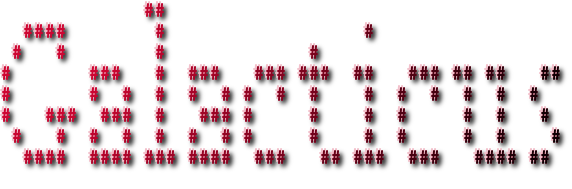
\includegraphics[width=125mm]{GalacticusLogo.png}\\

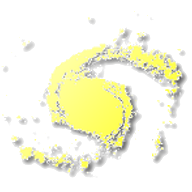
\includegraphics{New_Logo_Galaxy_192_Transparent.png}\\
A semi-analytic galaxy formation code.\\

\copyright\ 2009, 2010 2011, 2012, 2013, 2014, Andrew Benson
\end{center}

\tableofcontents

\mainmatter
\pagestyle{headings}

\part{Installation and Basic Use}

\chapter{About Galacticus}

\glc\ is a semi-analytic model of galaxy formation. It solves equations describing how galaxies evolve in a merging hierarchy of dark matter halos in a cold dark matter universe. \glc\ has much in common with other semi-analytic models, such as the range of physical processes included and the type of quantities that it can predict.

In designing \glc\ our main goal was to make the code flexible, modular and easily extensible. Much greater priority was placed on making the code easy to use and modify than on making it fast. We believe that a modular and extensible nature is crucial as galaxy formation is an evolving science. In particular, key design features are:
\begin{description}
 \item [Extensible methods for all functions:] Essentially all functions within \glc\ are designed to be extensible, meaning that you can write your own version and insert it into \glc\ easily. For example, suppose you want to use an improved functional form for the \gls{cdm} halo mass function. You would simply write a subroutine conforming to a specified template that computes this mass function and add a short directive (see \S\ref{sec:CodeDirectives}) in your code which explains to the build system how to insert this function in \glc. A recompile of the code will then incorporate your new function.

 \item [Extensible components for tree nodes:] The basic structure in \glc\ is a merger tree, which consists of a linked tree of nodes which have various properties. \glc\ works by evolving the nodes forwards in time subject to a collection of differential equations and other rules. Each node can contains an arbitrary number of \emph{components}. A component may be a dark matter halo, a galactic disk, a black hole etc. Each component may have an arbitrary number of \emph{properties} (some of which may be evolving, others of which can be fixed). \glc\ makes it easy to add additional components. For example, suppose you wanted to add a ``stellar halo'' components (consisting of stars stripped from satellite galaxies). To do this, you would write a module which specifies the following for this component:
 \begin{itemize}
  \item Number of properties;
  \item Interfaces to set and get property values and rates of change;
  \item ``Pipes'' which allow for flows of mass/energy/etc. from one component to another;
  \item Functions describing the differential equations which govern the evolution of the properties;
  \item Functions describing how the component responds to various events (e.g. the node becoming a satellite, a galaxy-galaxy merger, etc.);
  \item Auxiliary functions for handling outputs etc.
 \end{itemize}
 Short directives embedded in this module explain to the \glc\ build system how to incorporate the new component. A recompile will then build your new component into \glc. Typically, a new component can be created quickly by copying an existing one and modifying it as necessary. Furthermore, multiple implementations of a component are allowed. For example, \glc\ contains a component which is a Hernquist spheroid. You could add a de Vaucouler's spheroid component. A simple input parameter then allows you to select which implementation will be used in a given run.

 \item [Centralized ODE solver:] \glc\ evolves nodes in merger trees by calling an ODE solver which integrates forwards in time to solve for the evolution of the properties of each component in a node. This means that you do not need to provide explicit solutions for ODEs (in many cases such solutions are not available anyway) and timestepping is automatically handled to achieve a specified level of precision. The ODE solver allows for the evolution to be interrupted. A component may trigger an interrupt at any time and may do so for a number of reasons. A typical use is to actually create a component within a given node---for example when gas first begins to cool and inflow in a node the disk component must be created. Other uses include interrupting evolution when a merging event occurs.
\end{description}

\subsection{License}

Copyright 2009, 2010, 2011, 2012, 2013, Andrew Benson \href{mailto:abenson@carnegiescience.edu}{\normalfont \ttfamily <abenson@carnegiescience.edu>}\\

\glc\ is free software: you can redistribute it and/or modify
it under the terms of the GNU General Public License as published by
the Free Software Foundation, either version 3 of the License, or
(at your option) any later version.

\glc\ is distributed in the hope that it will be useful,
but WITHOUT ANY WARRANTY; without even the implied warranty of
MERCHANTABILITY or FITNESS FOR A PARTICULAR PURPOSE.  See the
GNU General Public License for more details.

You should have received a copy of the GNU General Public License
along with \glc.  If not, see \href{http://www.gnu.org/licenses/}{\normalfont \ttfamily <http://www.gnu.org/licenses/>}.


\chapter{Installation}

\section{Binaries}

If you just want to run \glc, and don't want to modify the code in any way you can try using a standalone binary copy of \glc. This is often a good way to try out \glc\ without the overhead of installing libraries and tools required to compile \glc. Binaries can be found at the \href{https://sites.google.com/site/galacticusmodel/downloads}{download page} and are currently available only for x86\_64 Linux. The binary is updated every night to reflect any updates to \glc.

\section{Installation Scripts}

Installing all the tools required for \glc\ can take some time. To make this process easier we've developed some simple installation scripts for Ubuntu, Fedora and Red Hat flavors of Linux. You can find these at the \href{https://sites.google.com/site/galacticusmodel/downloads}{download page}, with discussion of their use at the \href{https://sites.google.com/site/galacticusmodel/downloads/installtion-scripts}{installation scripts} page. These should be run as root and will attempt to install everything need to run \glc. We suggest that you look through the scripts to see what they're doing before running them---we make no guarantees that they won't install something that breaks other aspects of your system---use them at your own risk!

\section{Required Libraries and Tools}

We run \glc\ on \href{http://fedoraproject.org/}{Fedora} Linux primarily. Installation instructions below are general, but we give some examples that are specific to Fedora (they probably work on other \href{http://yum.baseurl.org/}{{\normalfont \ttfamily yum}}-based Linux distributions though). For other distributions/OSs you'll need to figure out how to install pre-built packages or else install from source. We list tools and libraries in three categories: ``essential'', ``typical'' and ``full''. Essential tools are those required to compile and run \glc. Typical tools includes those additionally needed for common analysis tasks. The full set of tools allows you to run any of the scripts/programs included with \glc. The order in which tools are listed is the suggested order for installation---some tools depend on others which should therefore be installed first.

\subsection{Essential Requirements}\label{sec:requirementsEssential}

\begin{description}
 \item [Perl] The Perl language is a part of every Linux distribution that we know of, so use whatever method your distribution prefers to install it if you don't already have it. On Fedora the following (as root) will install Perl:
\begin{verbatim}
yum install perl
\end{verbatim}
If you need to install from source visit \href{http://www.perl.org/}{\normalfont \ttfamily http://www.perl.org/} and follow the instructions given there. We currently use Perl v5.12.4, although earlier versions may work (for compiling \glc\ we have had success with versions as early as 5.8.8---you can use {\normalfont \ttfamily perl -v} to discover which version of Perl you have installed).

\item [GNU Make] \glc\ uses \href{http://www.gnu.org/software/make/}{GNU Make} to build executables. Other implementations of {\normalfont \ttfamily make} may work, but we make no guarantees. On Fedora the following (as root) will install GNU Make:
\begin{verbatim}
yum install make
\end{verbatim}
Alternatively, GNU Make can be downloaded and installed from source as described online.

\item [GFortran] \glc\ is written primarily in Fortran using various aspects of the Fortran 2003 specification. We use \href{http://gcc.gnu.org/fortran/}{GNU Fortran} to compile \glc. You can use other Fortran compilers, but we make no claims as to whether they will support all required features of the Fortran language, or that they will produce correctly working code. On Fedora the following (as root) will install GNU Fortran:
\begin{verbatim}
yum install gcc-gfortran
\end{verbatim}
Alternatively, GNU Fortran can be downloaded and installed from source as described online. Note that \glc\ requires v7.0.0 or later of {\normalfont \ttfamily gcc-gfortran}---earlier versions \emph{will not work}\footnote{We cannot predict if significantly later versions of GNU Fortran will successfully compile \protect\glc.}.

\item [g++] \glc\ contains some C++ components. We use \href{http://gcc.gnu.org/projects/cxx0x.html}{GNU C++} to compile \glc. You can use other C++ compilers, but we make no claims as to whether they will produce correctly working code. On Fedora the following (as root) will install GNU C++:
\begin{verbatim}
yum install gcc-c++
\end{verbatim}
Alternatively, GNU C++ can be downloaded and installed from source as described online.

\item [GNU Scientific Library] The \href{http://www.gnu.org/software/gsl/}{GNU Scientific Library} (GSL) is used extensively by \glc\ to perform numerous numerical functions. We currently use v1.15 of GSL---earlier versions will not work (due to \glc's use of the {\normalfont \ttfamily odeiv2} ODE solver interface that was introduced in GSL v1.15). On Fedora the following (as root) will install GSL:
\begin{verbatim}
yum install gsl gsl-devel
\end{verbatim}
Alternatively, GSL can be downloaded and installed from source as described online.

\item [FoX] \href{http://uszla.me.uk/space/software/FoX/}{FoX} is an XML parser for Fortran. The source can be downloaded from \newline\href{http://www1.gly.bris.ac.uk/~walker/FoX/source/FoX-4.1.1-full.tar.gz}{\normalfont \ttfamily http://www1.gly.bris.ac.uk/\textasciitilde{}walker/FoX/source/FoX-4.1.1-full.tar.gz}. We recommend following the instructions provided with the download for install. We use FoX v4.1.0.

\item [HDF5] The \href{http://www.hdfgroup.org/HDF5/}{HDF5} specification is used for storing output data from \glc. We currently use HDF5\footnote{Early versions of HDF5 may work, but versions prior to v1.8.5 have known memory leak problems.} v1.8.8. On Fedora the following (as root) will install the HDF5 libraries:
\begin{verbatim}
yum install hdf5 hdf5-devel
\end{verbatim}
Alternatively, HDF5 can be downloaded and installed from source. If this is done, we recommend the following build sequence:
\begin{verbatim}
 F9X=gfortran
 export F9X
 ./configure --prefix=/usr/local --enable-fortran --enable-production
 make
 make check
 make install
\end{verbatim}

\item [FGSL] \href{http://www.lrz-muenchen.de/services/software/mathematik/gsl/fortran/}{FGSL} is a Fortran interface to the GNU Scientific Library and is used extensively by \glc. It can be downloaded from the link above. We use FGSL v0.9.4 and recommend the following build sequence. 
\begin{verbatim}
 ./configure --f90 gfortran
 make
 make install
\end{verbatim}

\item [CPAN] \glc\ requires some Perl modules which probably are not installed by default. We recommend that you install these via \href{http://www.cpan.org/}{CPAN} which probably is installed by default. If it is not, on Fedora the following (as root) will install CPAN:
\begin{verbatim}
yum install perl-CPAN
\end{verbatim}
Note that you can check if any of the following Perl modules are already installed using
\begin{verbatim}
 perl -e "use Module::Name"
\end{verbatim}
If no error message is given, the module is already installed. When installing modules using CPAN (see below for example), if the install fails because of a failed test, you can often force the install by running {\normalfont \ttfamily perl -MCPAN -e 'force("install","Module::Name")'}. Of course, this may mean that the module is not working correctly\ldots

\item [\href{http://search.cpan.org/~rgarcia/Switch-2.16/Switch.pm}{{\normalfont \ttfamily Switch }}] This module implements distributed conditional testing. It is part of the core Perl distribution up to Perl v5.12.0. From Perl v5.14.0 onward it must be installed using
\begin{verbatim}
perl -MCPAN -e 'install Switch'
\end{verbatim}

\item [\href{http://search.cpan.org/~grantm/XML-Simple-2.18/lib/XML/Simple.pm}{{\normalfont \ttfamily XML::Simple}}] Provides a simple interface in Perl for processing XML files. It is used extensively by \glc\ for building the code and for handling various data files. On Fedora the following (as root) will install {\normalfont \ttfamily XML::Simple}:
\begin{verbatim}
yum install perl-XML-Simple
\end{verbatim}
Alternatively, it can be installed from CPAN using:
\begin{verbatim}
perl -MCPAN -e 'install XML::Simple'
\end{verbatim}

\item [\href{http://search.cpan.org/~adamk/List-MoreUtils-0.33/lib/List/MoreUtils.pm}{{\normalfont \ttfamily List::MoreUtils}}] Provides additional list-oriented utilities in Perl. It is used when automatically constructing lists of parameters that are accepted by a given executable when that executable is compiled. On Fedora the following (as root) will install {\normalfont \ttfamily List::MoreUtils}:
\begin{verbatim}
yum install perl-List-MoreUtils
\end{verbatim}
Alternatively, it can be installed from CPAN using:
\begin{verbatim}
perl -MCPAN -e 'install List::MoreUtils'
\end{verbatim}

\item [\href{http://search.cpan.org/~jfitz/List-Uniq-0.20/lib/List/Uniq.pm}{{\normalfont \ttfamily List::Uniq}}] Provides functionality to find unique items in lists in Perl. It is used in \glc's build system. It can be installed from CPAN using:
\begin{verbatim}
perl -MCPAN -e 'install List::Uniq'
\end{verbatim}

\item [\href{http://search.cpan.org/~grantm/XML-SAX-0.99/SAX.pm}{{\normalfont \ttfamily XML::SAX}}] Provides functionality to parse XML in Perl. It is used in \glc's build system. On Fedora the following (as root) will install {\normalfont \ttfamily XML::SAX}:
\begin{verbatim}
yum install perl-XML-SAX
\end{verbatim}
Alternatively, it can be installed from CPAN using:
\begin{verbatim}
perl -MCPAN -e 'install XML::SAX
\end{verbatim}

\item [\href{http://search.cpan.org/~samtregar/XML-Validator-Schema-1.08/Schema.pm}{{\normalfont \ttfamily XML::Validator::Schema}}] Provides functionality to validate XML in Perl. It is used in \glc's build system to validate the \gls{component} \gls{dsl}. It can be installed from CPAN using:
\begin{verbatim}
perl -MCPAN -e 'install XML::Validator::Schema
\end{verbatim}

\item [\href{http://search.cpan.org/~kstephens/Data-Match-0.06/lib/Sort/Topological.pm}{{\normalfont \ttfamily Sort::Topological }}] This module implements dependency based sort and is used by the \glc\ build system to ensure that tasks are performed in the correct order. It can be installed using
\begin{verbatim}
perl -MCPAN -e 'install Sort::Topological'
\end{verbatim}

\item [\href{http://search.cpan.org/~drolsky/DateTime-0.70/lib/DateTime.pm}{{\normalfont \ttfamily Date::Time }}] This module implements handling of dates and times and is used by various scripts to timestamp files that they create. It can be installed using
\begin{verbatim}
perl -MCPAN -e 'install Date::Time'
\end{verbatim}

\item [\href{http://search.cpan.org/~smueller/Data-Dumper-2.131/Dumper.pm}{{\normalfont \ttfamily Data::Dumper }}] This module provides formatted output of arbitrary data structures. On Fedora the following (as root) will install {\normalfont \ttfamily Date::Time}:
\begin{verbatim}
yum install perl-DateTime
\end{verbatim}
Alternatively, it can be installed from CPAN using:
\begin{verbatim}
perl -MCPAN -e 'install Data::Dumper'
\end{verbatim}

\item [\href{http://search.cpan.org/~abigail/Regexp-Common-2017060201/lib/Regexp/Common.pm}{{\normalfont \ttfamily Regexp::Common }}] This module provides additional regular expression functoinality. On Fedora the following (as root) will install {\normalfont \ttfamily Regexp::Common}:
\begin{verbatim}
yum install perl-Regexp-Common
\end{verbatim}
Alternatively, it can be installed from CPAN using:
\begin{verbatim}
perl -MCPAN -e 'install Regexp::Common
\end{verbatim}

\item [\href{http://search.cpan.org/~dcantrell/NestedMap-1.0/lib/NestedMap.pm}{{\normalfont \ttfamily NestedMap}}] This module provides functionality for nested map operators within Perl. It can be installed from CPAN using:
\begin{verbatim}
perl -MCPAN -e 'install NestedMap'
\end{verbatim}
\end{description}

\subsection{Typical Requirements}\label{sec:requirementsTypical}

In addition to the tools listed in \S\ref{sec:requirementsEssential} a typical install (allowing you to run typical analysis tasks for example) requires the following tools to be installed:

\begin{description}
\item [\href{http://search.cpan.org/~chm/PDL-IO-HDF5-0.6501/hdf5.pd}{{\normalfont \ttfamily PDL::IO::HDF5}}] Provides a simple Perl interface to HDF5 files. It is used by analysis scripts to extract data from \glc\ output files. It can be installed from CPAN using:
\begin{verbatim}
 perl -MCPAN -e 'install PDL::IO::HDF5'
\end{verbatim}

\item [poppler] \href{http://poppler.freedesktop.org/}{poppler} is a set of tools for working with PDF files. We use v0.22.2 and recommend the following build sequence. 
\begin{verbatim}
 ./configure
 make
 make check
 make install
\end{verbatim}

  \item [\href{http://perldoc.perl.org/IO/Compress/Bzip2.html}{{\normalfont \ttfamily IO::Compress::Bzip2}}] This module provides the {\normalfont \ttfamily bzip2} compression tool in Perl. On Fedora the following (as root) will install {\normalfont \ttfamily IO::Compress::Bzip2}:
\begin{verbatim}
yum install perl-Compress-Bzip2
\end{verbatim}
Alternatively, it can be installed from CPAN using:
\begin{verbatim}
perl -MCPAN -e 'install IO::Compress::Bzip2'
\end{verbatim}

  \item [\href{http://search.cpan.org/~dconway/IO-Prompt-0.997002/lib/IO/Prompt.pm}{{\normalfont \ttfamily IO::Prompt}}] This module provides convenient reading from the prompt in Perl. On Fedora the following (as root) will install {\normalfont \ttfamily IO::Prompt}:
\begin{verbatim}
yum install perl-IO-prompt
\end{verbatim}
Alternatively, it can be installed from CPAN using:
\begin{verbatim}
perl -MCPAN -e 'install IO::Prompt
\end{verbatim}

  \item [\href{http://search.cpan.org/~bdfoy/IO-Interactive-0.0.6/lib/IO/Interactive.pm}{{\normalfont \ttfamily IO::Interactive}}] This module provides functionality to determine if a Perl script is running interactively. It can be installed from CPAN using:
\begin{verbatim}
perl -MCPAN -e 'install IO::Interactive
\end{verbatim}

  \item [\href{http://search.cpan.org/~anno/Text-Table-1.114/lib/Text/Table.pm}{{\normalfont \ttfamily Text::Table}}] This module provides formatted table output in Perl. On Fedora the following (as root) will install {\normalfont \ttfamily Text::Table}:
\begin{verbatim}
yum install perl-Text-Table
\end{verbatim}
Alternatively, it can be installed from CPAN using:
\begin{verbatim}
perl -MCPAN -e 'install Text::Table'
\end{verbatim}

  \item [\href{http://search.cpan.org/~mjd/Text-Template-1.46/lib/Text/Template.pm}{{\normalfont \ttfamily Text::Template}}] This module provides generation of templated text in Perl. On Fedora the following (as root) will install {\normalfont \ttfamily Text::Template}:
\begin{verbatim}
yum install perl-Text-Template
\end{verbatim}
Alternatively, it can be installed from CPAN using:
\begin{verbatim}
perl -MCPAN -e 'install Text::Template'
\end{verbatim}

  \item [\href{http://search.cpan.org/~rgarcia/Sub-Identify-0.12/lib/Sub/Identify.pm}{{\normalfont \ttfamily Sub::Identify}}] This module provides function names from function references in Perl. On Fedora the following (as root) will install {\normalfont \ttfamily Sub::Identify}:
\begin{verbatim}
yum install perl-Sub-Identify
\end{verbatim}
Alternatively, it can be installed from CPAN using:
\begin{verbatim}
perl -MCPAN -e 'install Sub::Identify'
\end{verbatim}

\item [\href{http://search.cpan.org/~jhi/perl-5.8.0/lib/Text/Wrap.pm}{{\normalfont \ttfamily Text::Wrap}}] This module provides formatted paragraph output in Perl. It is most likely part of a standard Perl install, but if not it can be installed from CPAN using:
\begin{verbatim}
perl -MCPAN -e 'install Text::Wrap
\end{verbatim}
\item [\href{http://pdl.perl.org/}{{\normalfont \ttfamily PDL}}] Provides array math handling in Perl. It is used extensively by \glc\ for analysis of models. On Fedora the following (as root) will install {\normalfont \ttfamily PDL}:
\begin{verbatim}
yum install perl-PDL
\end{verbatim}
Alternatively, it can be installed from CPAN using:
\begin{verbatim}
perl -MCPAN -e 'install PDL'
\end{verbatim}

\item [\href{http://search.cpan.org/dist/PDL-NiceSlice/NiceSlice.pm}{{\normalfont \ttfamily PDL::NiceSlice}}] Provides convenient array slicing for PDL. {\normalfont \ttfamily PDL::NiceSlice} can be installed from CPAN using:
\begin{verbatim}
perl -MCPAN -e 'install PDL::NiceSlice'
\end{verbatim}

item [\href{http://search.cpan.org/~sbeck/Math-SigFigs-1.09/lib/Math/SigFigs.pod}{{\normalfont \ttfamily Math::SigFigs}}] Provides formatting of numbers to a given number of significant figures. It is used by \glc\ when making plots. It can be installed from CPAN using:
\begin{verbatim}
perl -MCPAN -e 'install Math::SigFigs'
\end{verbatim}

\item [\href{http://search.cpan.org/~djburke/Astro-Cosmology-0.90/Cosmology.pm}{{\normalfont \ttfamily Astro::Cosmology}}] Provides basic cosmological calculations. It is used by \glc\ when making plots to convert data points measured under the assumptions of one set of cosmological parameters to the cosmological parameters assumed by \glc. It can be installed from CPAN using:
\begin{verbatim}
perl -MCPAN -e 'force("install","Astro::Cosmology")'
\end{verbatim}
\end{description}

\subsection{Full Requirements}\label{sec:requirementsFull}

In addition to the tools listed in \S\ref{sec:requirementsEssential} and \S\ref{sec:requirementsTypical} a full install (allowing you to run all scripts and programs included with \glc) requires the following tools to be installed:

\begin{description}
\item [\href{http://search.cpan.org/~andrewf/LaTeX-Encode-0.03/lib/LaTeX/Encode.pm}{{\normalfont \ttfamily LaTeX::Encode }}] This module formats text for output to a \LaTeX\ document. It can be installed using\footnote{On some systems, {\normalfont \ttfamily LaTeX::Encode} seems to have problems. Once installed, try executing: {\normalfont \ttfamily perl -e ``use LaTeX::Encode''}. If this issues any error messages, then you should locate the {\normalfont \ttfamily LaTeX\/Encode.pm} file on your system edit it to comment out (or remove) the ``{\normalfont \ttfamily use strict;}'' line.}
\begin{verbatim}
perl -MCPAN -e 'install LaTeX::Encode'
\end{verbatim}
  \item [\href{http://search.cpan.org/~jesse/perl-5.12.1/lib/File/Find.pm}{{\normalfont \ttfamily File::Find}}] This module provides functionality for searching directory structures for files. It can be installed from CPAN using:
\begin{verbatim}
perl -MCPAN -e 'install File::Find'
\end{verbatim}
  \item [\href{http://search.cpan.org/~jesse/perl-5.12.1/lib/File/Copy.pm}{{\normalfont \ttfamily File::Copy}}] This module provides interfaces for copying and moving files in Perl. It can be installed from CPAN using:
\begin{verbatim}
perl -MCPAN -e 'install File::Copy'
\end{verbatim}
  \item [\href{http://search.cpan.org/~jcristy/PerlMagick-6.59/Magick.pm}{{\normalfont \ttfamily Image::Magick}}] This module provides access to the {\normalfont \scshape ImageMagick} tools from Perl. On Fedora the following (as root) will install {\normalfont \ttfamily Image::Magick}:
\begin{verbatim}
yum install ImageMagick-perl
\end{verbatim}
Alternatively, it can be installed from CPAN using:
\begin{verbatim}
perl -MCPAN -e 'install Image::Magick'
\end{verbatim}

  \item [\href{http://search.cpan.org/dist/TermReadKey/ReadKey.pm}{{\normalfont \ttfamily Term::ReadKey}}] This module provides a simple interface for accepting key reads from standard input in Perl. On Fedora the following (as root) will install {\normalfont \ttfamily Term::ReadKey}:
\begin{verbatim}
yum install perl-TermReadKey
\end{verbatim}
Alternatively, it can be installed from CPAN using:
\begin{verbatim}
perl -MCPAN -e 'install Term::ReadKey'
\end{verbatim}
  \item [\href{http://search.cpan.org/~rjbs/MIME-Lite-3.027/lib/MIME/Lite.pm}{{\normalfont \ttfamily MIME::Lite}}] This module provides simple e-mail sending functionality in Perl. On Fedora the following (as root) will install {\normalfont \ttfamily MIME::Lite}:
\begin{verbatim}
yum install perl-MIME-Lite
\end{verbatim}
Alternatively, it can be installed from CPAN using:
\begin{verbatim}
perl -MCPAN -e 'install MIME::Lite'
\end{verbatim}
  \item [\href{http://search.cpan.org/~gbarr/TimeDate-1.20/lib/Date/Format.pm}{{\normalfont \ttfamily Date::Time}}] This module provides date/time formatting functionality in Perl. On Fedora the following (as root) will install {\normalfont \ttfamily Date::Time}:
\begin{verbatim}
yum install perl-DateTime
\end{verbatim}
Alternatively, it can be installed from CPAN using:
\begin{verbatim}
perl -MCPAN -e 'install Date::Format'
\end{verbatim}
  \item [\href{http://search.cpan.org/~cwest/Net-SMTP-SSL-1.01/lib/Net/SMTP/SSL.pm}{{\normalfont \ttfamily Net::SMTP::SSL}}] This module implements an SSL authenticated SMTP e-mail protocol in Perl. On Fedora the following (as root) will install {\normalfont \ttfamily Net::SMTP::SSL}:
\begin{verbatim}
yum install perl-Net-SMTP-SSL
\end{verbatim}
Alternatively, it can be installed from CPAN using:
\begin{verbatim}
perl -MCPAN -e 'install Net::SMTP::SSL'
\end{verbatim}

\item [\href{http://search.cpan.org/~danberr/Net-DBus-0.33.6/lib/Net/DBus.pm}{{\normalfont \ttfamily Net::DBus}}] This module implements interaction with the \href{http://www.freedesktop.org/wiki/Software/dbus}{DBus} message bus system in Perl. On Fedora the following (as root) will install {\normalfont \ttfamily Net::DBus}:
\begin{verbatim}
yum install perl-Net-DBus
\end{verbatim}
Alternatively, it can be installed from CPAN using:
\begin{verbatim}
perl -MCPAN -e 'install Net::DBus'
\end{verbatim}

\item [\href{http://search.cpan.org/~dexter/POSIX-strftime-GNU-0.02/lib/POSIX/strftime/GNU.pm}{{\normalfont \ttfamily POSIX::strftime::GNU}}] This module implements character sequences compatible with GNU systems. It can be installed from CPAN using:
\begin{verbatim}
perl -MCPAN -e 'install POSIX::strftime::GNU'
\end{verbatim}

  \item [\href{http://search.cpan.org/~chm/PDL-2.4.7/Basic/MatrixOps/matrixops.pd}{{\normalfont \ttfamily PDL::MatrixOps}}] Provides matrix operators for PDL. It is used when generating Monte Carlo samples of parameters from covariance matrices. {\normalfont \ttfamily PDL::MatrixOps} can be installed from CPAN using:
\begin{verbatim}
perl -MCPAN -e 'install PDL::MatrixOps'
\end{verbatim}
  \item [\href{http://search.cpan.org/~ellipse/PDL-LinearAlgebra-0.06/LinearAlgebra.pm}{{\normalfont \ttfamily PDL::LinearAlgebra}}] Provides linear algebra algorithms for PDL. It is used for Cholesky decomposition when generating Monte Carlo samples of parameters from covariance matrices. {\normalfont \ttfamily PDL::LinearAlgebra} can be installed from CPAN using:
\begin{verbatim}
perl -MCPAN -e 'install PDL::LinearAlgebra'
\end{verbatim}

\item[Gnuplot] The \href{http://www.gnuplot.info/}{\normalfont \scshape Gnuplot} plotting package is used extensively by \glc\ to produce plots. While not required for running \glc\ it is recommended as it allows you to easily check model results using the preexisting plotting scripts. On Fedora the following (as root) will install {\normalfont \ttfamily Gnuplot}:
\begin{verbatim}
yum install gnuplot
\end{verbatim}
Alternatively, {\normalfont \scshape Gnuplot} can be installed from source, following the online instructions. Note that some scripts require {\normalfont \scshape Gnuplot} v4.4 or later.

\item[GraphViz] The \href{http://www.graphviz.org/}{GraphViz} package is used to create plots of merger tree structures. While not required to run \glc\ it is recommended to allow simple graphing of such structures (useful to get a visual impression of what's going on in the code). On Fedora the following (as root) will install GraphViz and a module that allows Perl to interact with it:
\begin{verbatim}
yum install graphviz perl-GraphViz
\end{verbatim}
Alternatively, GraphViz can be installed from source, following the online instructions, while the Perl module can be installed from CPAN using
\begin{verbatim}
perl -MCPAN -e 'install GraphViz'
\end{verbatim}

\end{description}

\subsection{Optional Requirements}

\glc\ can make use of the \gls{yeppp} library for for optimized vector math operations\footnote{At present, usage of \protect\gls{yeppp} is limited to numerical integration routines, but these are as yet not utilized within the code.}. To link \glc\ with \gls{yeppp} simply install \gls{yeppp} following their instructions, and ensure that the \gls{yeppp} environment variables are set. \glc\ will detect the \gls{yeppp} installation via this environment variables and will adjust its build appropriately.

\section{Compiling Galacticus}

To build \glc\ (after installing all required libraries) ensure that you are in the {\normalfont \ttfamily Galacticus/v0.0.1} directory and then simply type:
\begin{verbatim}
 make Galacticus.exe
\end{verbatim}
This will create the {\normalfont \ttfamily Galacticus.exe} executable. The build takes some time, you'll see a set of XML files get created first which \glc\ uses to figure out how modules link in to the \glc\ code. After that, the Fortran files are compiled. We regularly build \glc\ using a parallel make without any problems.

The {\normalfont \ttfamily Makefile} contains a few options that you may want to adjust:
\begin{description}
 \item[{\normalfont \ttfamily FCCOMPILER}] The command to invoke a Fortran 2003 compliant compiler. \glc\ should compile with any such compiler. In practice, we have only tried it using {\normalfont \scshape GFortran} v7.0.0+\footnote{We cannot predict if significantly later versions of GNU Fortran will successfully compile \protect\glc.}. In particular, \glc\ makes use of certain Fortran 2003 features (notably procedure pointers, type-bound procedures and class variables) which older compilers might not handle (and some newer compilers might still have difficulty with);
 \item[{\normalfont \ttfamily CCOMPILER}] The command to invoke a C compiler.
 \item[{\normalfont \ttfamily CPPCOMPILER}] The command to invoke a C++ compiler.
 \item[{\normalfont \ttfamily PREPROCESSOR}] The command to invoke a preprocessor to handle {\normalfont \ttfamily \#IFDEF} etc. statements. We normally use {\normalfont \ttfamily cpp};
 \item[{\normalfont \ttfamily MODULETYPE}] A label identifying the structure of modules built by the compiler. This is used to detected when module interfaces have been changed (requiring a recompile of all dependent code) and when only the module internals have changed. When the {\normalfont \scshape GFortran} compiler is used {\normalfont \ttfamily GCC-f95-on-LINUX} should be used here. Look in {\normalfont \ttfamily ./scripts/build/Compare\_Module\_Files.pl} for other possibilities (if your compiler isn't listed you'll need to either edit that script or deal with longer recompiles if you edit the code).
 \item[{\normalfont \ttfamily FCFLAGS}] Flags to pass to the Fortran compiler. Standard options for both error-checking and optimized builds for the {\normalfont \scshape GFortran} compiler are given in the {\normalfont \ttfamily Makefile}.
 \item[{\normalfont \ttfamily CFLAGS}] Flags to pass to the C compiler.
 \item[{\normalfont \ttfamily CPPFLAGS}] Flags to pass to the C++ compiler.
\end{description}
Additionally, you can add compiler options to the {\normalfont \ttfamily GALACTICUS\_FCFLAGS}, {\normalfont \ttfamily GALACTICUS\_CFLAGS}, and {\normalfont \ttfamily GALACTICUS\_CPPFLAGS} environment variables. This is useful to add machine-specific options.

\subsection{Compiling with OpenMP Parallelism}\index{OpenMP}\index{parallel}

By default, \glc\ will be compiled to run in parallel on machine with multiple CPUs using \href{http://openmp.org/wp/}{OpenMP}. To disable this simply remove (or comment out the)
\begin{verbatim}
FCFLAGS += -fopenmp
\end{verbatim}
line in the Makefile. When running \glc\ in parallel using OpenMP it may be necessary to increase the stack size allocated to each thread (since \glc\ calls some procedures recursively this can result in large numbers of local variables being allocated on the stack). To do this, use
\begin{verbatim}
setenv KMP_STACKSIZE 16777216
\end{verbatim}
in {\normalfont \ttfamily csh} and variants or
\begin{verbatim}
export KMP_STACKSIZE=16777216
\end{verbatim}
in {\normalfont \ttfamily bash} and variants. If you get stack overflows while running \glc\ in parallel, try increasing this value further.

\glc\ currently implements parallel calculations at the tree level---that is, each parallel thread works on a separate merger tree. This means that you need sufficient memory to hold multiple merger trees at once. The advantage of this approach is that it is highly scalable (assuming no need for communication between trees), and \glc\ can achieve close to optimal speed-up in many cases. The limit to the speed-up is usually determined by the workload balance between the trees. If one tree requires significantly more time to run that all other trees combined then one thread will be left working on that tree while all others have finished. To limit this problem, it is recommended that parallel runs which use {\normalfont \ttfamily mergerTreeConstructMethod}$=${\normalfont \ttfamily build} (see \S{sec:MergerTreeConstruction}) be conducted with the {\normalfont \ttfamily [mergerTreeBuildTreesProcessDescending]}$=${\normalfont \ttfamily true} parameter set to true. This will cause the most massive merger trees (i.e. those which take longest to process) to be processed first.

\subsection{Compiling with MPI Parallelism}\index{MPI}\index{parallel}

While \glc\ currently does not support \gls{mpi} parallelism, certain other codes included with \glc\ do. To compile such a code use
\begin{verbatim}
make GALACTICUS_BUILD_OPTION=MPI Constrain_Galacticus.exe
\end{verbatim}
for example. The {\tt GALACTICUS\_BUILD\_OPTION=MPI} option instructs the build system to compile all codes into the {\tt work/buildMPI} directory, and define a {\tt USEMPI} preprocessor macro to allow the compiled code to be modified appropriately for \gls{mpi}. Note that you must have a working \gls{mpi} installed of course.

\section{Installing Without Root Access}

It is possible to install \glc\ without root access to your computer. The following approach has worked in many cases---some adjustments may be required for your specific system. Depending on what is already installed on your system, you may be able to skip some of the following installs. Refer to \S\ref{sec:requirementsEssential}, \S\ref{sec:requirementsTypical} and \S\ref{sec:requirementsFull} to decide which of the following tools you want to install. (Or, alternatively, you may need to install additional tools.) Choose a location to install that has at least 4Gb of free space. In the following, this install location is referred to as {\normalfont \ttfamily /your/install/path}. In the following, we assume you're using some variant of the C-shell. If you're using {\normalfont \ttfamily bash} or some other Bourne shell, {\normalfont \ttfamily setenv VAR abcd} should be translated to {\normalfont \ttfamily export VAR=abcd}.

\lstdefinelanguage{simple}{morecomment=[l]!}
\begin{lstlisting}[language=simple,stringstyle=\normalfont \ttfamily,commentstyle=\itshape]

! Install GFortran, GCC and G++:

svn co svn://gcc.gnu.org/svn/gcc/trunk gcc-trunk
cd gcc-trunk
svn up
cd ..
rm -rf gcc-build
mkdir gcc-build
cd gcc-build
../gcc-trunk/configure --prefix=/your/install/path --enable-languages=c,c++,fortran --disable-multilib
make
make install

! Add to .cshrc (or equivalent):

setenv PATH /your/install/path/bin:$PATH                                                                                           
setenv LD_LIBRARY_PATH /your/install/path/lib:$LD_LIBRARY_PATH

! Install GSL:

wget "http://www.mirrorservice.org/sites/ftp.gnu.org/gnu/gsl/gsl-1.15.tar.gz"
tar xvfz gsl-1.15.tar.gz
cd  gsl-1.15
./configure --prefix=/your/install/path
make
make check
make install

! Install FGSL:

wget "http://www.lrz-muenchen.de/services/software/mathematik/gsl/fortran/\
fgsl-0.9.4.tar.gz"
tar xvfz fgsl-0.9.4.tar.gz
cd fgsl-0.9.4
./configure --f90 gfortran --gsl /your/install/path
make
make install

! Install zlib:

wget "http://zlib.net/zlib-1.2.5.tar.gz"
tar xvfz zlib-1.2.5.tar.gz
cd zlib-1.2.5
./configure --prefix=/your/install/path
make
make check
make install

! Install HDF5:

wget http://www.hdfgroup.org/ftp/HDF5/current/src/hdf5-1.8.7.tar.bz2
tar xvfz hdf5-1.8.7.tar.gz
cd hdf5-1.8.7
setenv F9X gfortran
./configure --prefix=/your/install/path --enable-fortran --enable-production \
 --with-zlib=/your/install/path
make
make check
make install

! Install FoX:

wget "http://www1.gly.bris.ac.uk/~walker/FoX/source/FoX-4.1.0-full.tar.gz"
tar xvfz FoX-4.1.0-full.tar.gz
cd FoX-4.1.0
setenv FC gfortran
./configure --prefix=/your/install/path
make
make check
make install

! Install Mercurial:

wget "http://mercurial.selenic.com/release/mercurial-2.4.1.tar.gz"
tar xvfz mercurial-2.4.1.tar.gz
cd mercurial-2.4.1
setenv PREFIX /your/install/path
make
make install

! Install Poppler:

wget "http://poppler.freedesktop.org/poppler-0.22.2.tar.gz"
tar xvfz poppler-0.22.2.tar.gz
cd poppler-0.22.2
./configure --prefix=/your/install/path
make
make check
make install

! Install Perl local::lib for local installs of modules:

mkdir .cpan
mkdir perl5
ln -sf /your/install/path/.cpan $HOME/
ln -sf /your/install/path/perl5 $HOME/
wget http://search.cpan.org/CPAN/authors/id/A/AP/APEIRON/local-lib-1.008004.tar.gz
tar xvfz local-lib-1.008004.tar.gz 
cd local-lib-1.008004
perl Makefile.PL --bootstrap
make
make test
make install
perl -I$HOME/perl5/lib/perl5 -Mlocal::lib >> $HOME/.cshrc

! Install Perl modules:

perl -MCPAN -e "install Sort::Topological"
perl -MCPAN -e "install LaTeX::Encode"
perl -MCPAN -e "install XML::Simple"
perl -MCPAN -e "install Math::SigFigs"
perl -MCPAN -e "install GraphViz"
perl -MCPAN -e "install File::Find"
perl -MCPAN -e "install File::Copy"
perl -MCPAN -e "install Image::Magick"
perl -MCPAN -e "install Term::ReadKey"
perl -MCPAN -e "install MIME::Lite"
perl -MCPAN -e 'install Regexp::Common'
perl -MCPAN -e 'install Text::Table'
perl -MCPAN -e 'install Text::Template'
perl -MCPAN -e 'install NestedMap'
perl -MCPAN -e 'install Sub::Identify'
perl -MCPAN -e 'install IO::Compress::Bzip2'
perl -MCPAN -e 'install Date::Format'
perl -MCPAN -e 'install Net::SMTP::SSL'
perl -MCPAN -e 'install Net::DBus'
perl -MCPAN -e 'install PDL'
perl -MCPAN -e 'install PDL::LinearAlgebra'
perl -MCPAN -e 'install PDL::MatrixOps'
perl -MCPAN -e 'install PDL::NiceSlice'
perl -MCPAN -e 'install PDL::IO::HDF5
perl -MCPAN -e 'force("install","Astro::Cosmology")'

! Install GnuPlot:

wget "http://downloads.sourceforge.net/project/gnuplot/gnuplot/4.4.3/gnuplot-4.4.3.tar.gz"
tar xvfz gnuplot-4.4.3.tar.gz
cd gnuplot-4.4.3
./configure --prefix=/your/install/path
make
make install

! Install GraphViz:

wget "http://www.graphviz.org/pub/graphviz/stable/SOURCES/graphviz-2.28.0.tar.gz"
tar xvfz graphviz-2.28.0.tar.gz
cd graphviz-2.28.0
./configure --prefix=/your/install/path
make
make check
make install

! Install Galacticus:

wget "http://users.obs.carnegiescience.edu/abenson/galacticus/versions/\
galacticus_v0.9.3.tar.bz2"
tar xvfj galacticus_v0.9.3.tar.bz2
cd Galacticus/v0.9.3

! Add to Makefile (below the GALACTICUS_FCFLAGS = line):

GALACTICUS_FCFLAGS += -fintrinsic-modules-path /your/install/path/finclude \
   -fintrinsic-modules-path /your/install/path/include/gfortran            \
   -fintrinsic-modules-path /your/install/path                             \
   -fintrinsic-modules-path /your/install/path/include                     \
   -L /your/install/path/lib
\end{lstlisting}

It should then be possible to compile and run \glc.

\section{Installing on Mac OS X}

The following guidelines have been tested on a MacBook Pro, running Mac OS X V10.6.8. 

\subsection{Update GNU compilers}

It is likely that the default compiler is older than GCC v7.0.0 that is required to properly compile the code without any errors. Use a package manager to download as recent a version as possible of {\normalfont \ttfamily gcc}. For the case of MacPorts, this requires,

\begin{verbatim}
$ sudo port -v install gcc48 +gfortran
\end{verbatim}

and reset the default version of {\normalfont \ttfamily gcc} compilers by first listing available options

\begin{verbatim}
$ sudo port select --list gcc
\end{verbatim}

and then explicitly setting to {\normalfont \ttfamily mp-gcc48} by

\begin{verbatim}
$ sudo port select --set mp-gcc48
\end{verbatim}

\subsection{Installing HDF5, FoX and FGSL}

Once you have installed the latest compiler suite, you will need to recompile your {\normalfont \ttfamily HDF5}, {\normalfont \ttfamily FoX} and {\normalfont \ttfamily FGSL} libraries. Download {\normalfont \ttfamily FoX} (for XML parsing) from

\begin{verbatim}
http://www1.gly.bris.ac.uk/~walker/FoX/source/FoX-4.1.2-full.tar.gz
\end{verbatim}

and run {\normalfont \ttfamily configure}

\begin{verbatim}
$ sudo ./configure --prefix=/opt/local
\end{verbatim}

i.e. install libraries in the same branch as the MacPorts distributiuon. Then do the usual

\begin{verbatim}
$ sudo make clean; sudo make; sudo make check; sudo make install
\end{verbatim}

Similarly download FGSL from

\begin{verbatim}
http://www.lrz.de/services/software/mathematik/gsl/fortran/
\end{verbatim}

and, assuming that you have downloaded GSL with MacPorts and they are installed in {\normalfont \ttfamily /opt/local/include} and {\normalfont \ttfamily /opt/local/lib}, run {\normalfont \ttfamily configure}

\begin{verbatim}
$ sudo ./configure --f90 gfortran --gsl /opt/local --prefix /opt/local
\end{verbatim}

i.e. install libraries in the same branch as the MacPorts distributiuon. Then do the usual

\begin{verbatim}
$ sudo make clean; sudo make; sudo make install
\end{verbatim}

Finally download the latest version of HDF5, configure

\begin{verbatim}
$ sudo ./configure --enable-fortran --prefix=/opt/local
\end{verbatim}

and do the usual

\begin{verbatim}
$ sudo make clean; sudo make; sudo make test; sudo make install
\end{verbatim}

This should ensure that the modules ({\normalfont \ttfamily hdf5.mod}, {\normalfont \ttfamily fox\_dom.mod}, \ldots) are compatible with the \glc\ build.

\glc\ requires {\normalfont \ttfamily crypt.h} to install on linux-based systems; this is part of the GNU C library {\normalfont \ttfamily glibc}. However, {\normalfont \ttfamily glibc} has not been ported to Mac OS X and so this will not work properly. To get it working, edit {\normalfont \ttfamily source/utility.hashes.cryptographic.md5.c} and comment out {\normalfont \ttfamily \#include \textless crypt.h\textgreater}, replacing it with {\normalfont \ttfamily \#include \textless unistd.h\textgreater}.

Note that you will need to amend the {\normalfont \ttfamily Makefile} so that \glc\ knows where these {\normalfont \ttfamily .mod} files are, which you can do by adding

\begin{verbatim}
FCFLAGS += -fintrinsic-modules-path /opt/local/include 
	   -fintrinsic-modules-path /opt/local/include/gfortran
	   -fintrinsic-modules-path /opt/local/finclude .
\end{verbatim}

You can also add

\begin{verbatim}
export GALACTICUS_FCFLAGS = "-L/opt/local/lib"
\end{verbatim}

You can also add

to your {\normalfont \ttfamily .profile} (i.e. {\normalfont \ttfamily .bashrc}) file so that \glc\ knows where to find libraries (for FoX, {\normalfont \ttfamily libcrypt}, \ldots) during linking.

\subsection{Installing Perl Modules}

Follow the instructions in the previous section to download and install new {\normalfont \ttfamily perl} modules. You may need to upgrade CPAN using

\begin{verbatim}
$ sudo perl -MCPAN -e 'install Bundles::CPAN'
\end{verbatim}

before installation of certain modules (e.g. {\normalfont \ttfamily DateTime.pm}) would proceed correctly. To install {\normalfont \ttfamily PDF::Labels}, I found it necessary to

\begin{verbatim}
$ sudo perl -MCPAN -e 'install PDF::Create"
\end{verbatim}

and then

\begin{verbatim}
$ sudo perl -MCPAN -e 'install PDF::Labels"
\end{verbatim}


\chapter{Running Galacticus}

\section{Configuration File}\label{sec:ConfigFile}\index{galacticusConfig.xml@{\tt galacticusConfig.xml}}\index{configuration}

The file {\tt galacticusConfig.xml}, is present, is used to configure \glc\ and provide useful information. It should have the following structure:
\begin{verbatim}
<config>
  <contact>
    <name>My Name</name>
    <email>me@ivory.towers.edu</email>
  </contact>
  <email>
    <host>
      <name>myComputerHostName</name>
      <method>smtp</method>
      <host>smtp-server.ivory.towers.edu</host>
      <user>myUserName</user>
      <passwordFrom>kdewallet</passwordFrom>
    </host>
    <host>
      <name>default</name>
      <method>sendmail</method>
    </host>
  </email>
</config>
\end{verbatim}
The name and e-mail address in the {\tt contact} section will be stored in any \glc\ models run---this helps track the provenance of the model. The {\tt email} section determines how e-mail will be sent. Within this section, you can place one or more {\tt host} elements, the {\tt name} element of which specifies the host name of the computer to which these rules apply (the {\tt default} host is used if no other match is found). For each host, the {\tt method} element specifies how e-mail should be sent, either by {\tt sendmail} or via {\tt smtp}. For SMTP transport (which currently supports SSL connections only), you must specify the {\tt host} SMTP server, {\tt user} name. The {\tt passwordFrom} element specifies how the password for the SMTP log in should be obtained. If set to {\tt input} then the user will be prompted for the password as needed. Alternatively, if you use the \href{http://www.kde.org/}{KDE} desktop and the \href{http://utils.kde.org/projects/kwalletmanager/}{KDEWallet} password manager, 
setting {\tt passwordFrom} to {\tt kdewallet} will cause the password to be stored in the KDE wallet and retrieved from there subsequently.

\section{Parameter Files}

\glc\ requires a file of parameters to be given as a command line argument. The parameter file is an XML file (which makes it easy to manipulate and construct these files from within many languages, e.g. Perl) with the following structure:
\begin{verbatim}
 <parameters>
   <parameter>
     <name>parameter1name</name>
     <value>parameter1value</value>
   </parameter>
   .
   .
   .
 </parameters>
\end{verbatim}
Each {\tt parameter} element contains {\tt name} and {\tt value} elements which contain the parameter name and desired value respectively. The value can be a number, word(s) or an array of space-separated numbers or words. Parameters are used to control the values of numerical parameters and also to select methods and other options. If a parameter is not specified in the file a default value (hard coded into \glc) will be used instead. The default values have been chosen to produce a realistic model of galaxy formation, but may change as \glc\ evolves.

All parameter values (both those specified in this file and those set to default) used during a \glc\ run are output to the {\tt Parameters} group within the \glc\ output file. The script {\tt scripts/aux/Extract\_Parameter\_File.pl} will, if given a \glc\ output file, extract the parameters from it and output them into an XML file suitable for re-input into \glc. If parameters are present in the parameter file which do not match any known parameter in \glc\ then a warning message, listing all unknown parameters, will be given when \glc\ is run. Note that this will \emph{not} prevent \glc\ from running---sometimes it is convenient to include parameters which are not used by \glc, but which might be used by some other code.

\subsection{Validating Parameter Files}\index{parameters!validating}

A script, {\tt scripts/aux/validateParameters.pl}, is provided to validate parameter files and thereby ensure that they are consistent with \glc's expectations and requirements. To use simply execute:
\begin{verbatim}
 scripts/aux/validateParameters.pl myParameters.xml
\end{verbatim}
No output (and an exit value of 0) indicates a valid parameter file. Invalid parameter files will result in an exit value other than 0 and will produce error messages that should help to track down the problem with the file.

\subsection{Generating Parameter Files}\index{parameters!generating}

Some scripts are provided which assist in the generation of parameter files. These are located in the {\tt scripts/parameters/} folder and are detailed below:
\begin{description}
\item [{\tt cosmologicalParametersMonteCarlo.pl}] This script will generate a set of cosmological parameters drawn at random from the WMAP-9 constraints \cite{hinshaw_nine-year_2012}. It uses the covariance matrix (currently defined in {\tt data/Cosmological\_Parameters\_WMAP-9.xml}) to produce correlated random variables\footnote{Note that this does not capture the full details of the correlations between parameters, since it uses just the covariance matrix. For a more accurate calculation the full Monte Carlo Markov Chains used in the WMAP-9 parameter fitting should be used instead.}. The generated parameters are printed to standard output as \glc-compatible XML.
\end{description}

\section{Running Galacticus}

\glc\ is running using
\begin{verbatim}
 Galacticus.exe [<parameterFile>]
\end{verbatim}
where {\tt parameterFile} is the name of the file containing a list of parameter values for \glc. \glc\ will display messages indicating its progress as it runs (the verbosity can be controlled with the {\tt verbosityLevel} parameter). Usually, the \glc\ executable should be invoked from the directory in which it was built. However, you can choose to set the environment variable {\tt GALACTICUS\_ROOT\_V091} to the full path to the build directory\index{path!galacticus root@{\glc\ root}}, in which case the \glc\ executable can be invoked from anywhere and will access all required files and scripts relative to this path. This can allow multiple users to all make use of the same \glc\ install.

\subsection{Writing Data To a Temporary File}\index{output!temporary}

When running \glc\ on a compute cluster it is often advantageous to have output written to a local scratch disk during run time and only moved to networked storage after the run is complete. (Otherwise, \glc\ will perform many small writes to networked storage which can result in extremely slow run times.) To do this, simply set the parameter {\tt [galacticusOutputScratchFileName]} to the full path of a file to write to on local scratch space. During the run, data will be written to this file. After the run is finished, \glc\ will move this file to its permanent location as specified by the parameter {\tt [galacticusOutputFileName]}.

\subsection{Restarting A Crashed Run}\label{sec:Restarting}

If \glc\ crashes, it can be useful to restart the calculation from just prior to the crash to speed the debugging process. \glc\ has functionality to store and retrieve the internal state of any modules and to recover this to permit such restarting. Currently, this is implemented with the {\tt build} and {\tt read} methods of merger tree construction, such that the internal state is stored prior to commencing the building or reading of each tree, thereby allowing a calculation to be restarted with the tree that crashed. More general store/retrieve behavior is planned for future releases.

To cause \glc\ to periodically store its internal state include the following input parameter:
\begin{verbatim}
  <parameter>
    <name>stateFileRoot</name>
    <value>galacticusState</value>
  </parameter>
\end{verbatim}
This will cause the internal state to be stored to files {\tt galacticusState.state} and {\tt galacticusState.fgsl.state} prior to commencing building each merger tree. Should a tree crash then replace this input parameter with:
\begin{verbatim}
  <parameter>
    <name>stateRetrieveFileRoot</name>
    <value>galacticusState</value>
  </parameter>
  <parameter>
    <name>mergerTreeBuildTreesBeginAtTree</name>
    <value>N</value>
  </parameter>
\end{verbatim}
where {\tt N} is the number of the tree that crashed. This will cause calculations to begin with tree {\tt N} and for the internal state to be recovered from the above mentioned files. The resulting tree and all galaxy formation calculations should therefore proceed just as in the original run (and so create the same crash condition).

\subsubsection{OpenMP}\index{debugging!OpenMP}\index{OpenMP!debugging}

When running a model in parallel using OpenMP, a separate state file will be written for each thread, with the thread number appended to the end of each state file name. For debugging purposes, it is suggested that a crashed OpenMP run be restarted using just a single thread. To do this, change the appended thread number on the state files corresponding to the thread which crashed to 0 such that they will be used by the single thread when the run is restarted.

\subsection{Running Grids of Models}\label{sec:RunningGrids}

You can easily write your own scripts to generate parameter files and run \glc\ on these files. An example of such a script is {\tt scripts/aux/launch.pl}. This script will loop over a sequence of parameter values, generate appropriate parameter files, run \glc\ using those parameters and analyze the results. This script currently supports running of \glc\ on a local machine, via a PBS queue (as multiple jobs or a single job), or on a \href{http://www.cs.wisc.edu/condor/}{{\sc Condor}}\index{Condor} cluster. To run the script simply enter:
\begin{verbatim}
 ./scripts/aux/launch.pl <runFile>
\end{verbatim}
This will launch a single instance of the script. Multiple instances can be launched and will share the work load (i.e. they will not attempt to run a model which another instance is already running or has finished). If multiple instances are to be launched on multiple machines a command line option to {\tt launch.pl} can be used to ensure that they do not duplicate work. Adding {\tt --instance 2:4} for example will tell the script to run only the second model from each block of four models it finds. Launching for {\tt launch.pl} scripts on four different machines with {\tt --instance 1:4}, {\tt --instance 2:4}, {\tt --instance 3:4} and {\tt --instance 4:4} will then divide the models between those machines.

The {\tt runFile} is an XML file with the following structure:
\begin{verbatim}
<parameterGrid>
 <modelRootDirectory>models.new</modelRootDirectory>
 <baseParameters>newBestParametersQuick.xml</baseParameters>
 <compressModels>no</compressModels>
 <splitModels>4</splitModels>

 <launchMethod>pbs</launchMethod>

  <local>
   <threadCount>3</threadCount>
   <ompThreads>4</ompThreads>
  </local>

 <condor>
  <galacticusDirectory>/home/condor/Galacticus/v0.9.3</galacticusDirectory>
  <universe>vanilla</universe>
  <environment>LD_LIBRARY_PATH=/usr/lib:/usr/lib64:/usr/local/lib</environment>
  <requirement>Memory &gt;= 1000 &amp;&amp; Memory &lt; 2000</requirement>
  <transferFile>{PWD}/myFile.data</transferFile>
  <wholeMachine>true</wholeMachine>
 </condor>

 <pbs>
  <scratchPath>/scratch/me</scratchPath>
  <wallTime>48:00:00</wallTime>
  <memory>3gb</memory>
  <ompThreads>8</ompThreads>
  <queue>standard</queue>
  <maxJobsInQueue>10</maxJobsInQueue>
  <mpiLaunch>yes</mpiLaunch>
  <mpiRun>/opt/openmpi/bin/mpirun</mpiRun>
  <environment>LD_LIBRARY_PATH=/home/me/software/Galacticus/Tools/lib64:$LD_LIBRARY_PATH</environment>                                                                   
 </pbs>                                                                                           
 <monolithicPBS>
  <mpiLaunch>yes</mpiLaunch>
  <nodes>1</nodes>
  <threadsPerNode>12</threadsPerNode>
  <ompThreads>6</ompThreads>
  <jobWaitSleepDuration>60</jobWaitSleepDuration>
  <analyze>no</analyze>
  <environment>LD_LIBRARY_PATH=/home/me/software/Galacticus/Tools/lib64:$LD_LIBRARY_PATH</environment>                                                                   
 </monolithicPBS>
                  
 <parameters>
  <label>modelLabel</label>
  <parameter>
   <name>stabilityThresholdStellar</name>
   <value>1.1</value>
   <value>0.9</value>
  </parameter>
 </parameters>
 <parameters>
  <parameter>
   <name>stabilityThresholdGaseous</name>
   <value>1.1</value>
   <value>0.9</value>
  </parameter>
  <parameter>
   <name>imfSalpeterYieldInstantaneous</name>
   <value>0.02</value>
   <value>0.04</value>
  </parameter>
  <parameter>
   <name>imfSelectionFixed</name>
   <value>Salpeter</value>
   <value>Chabrier</value>
  </parameter>
  <parameter>
   <name>starFormationTimescaleDisksMethod</name>
   <value>Kennicutt-Schmidt
    <parameter>
     <name>starFormationKennicuttSchmidtTruncate</name>
     <value>true</value>
     <value>false
     <parameter>
      <name>imfSelectionFixed</name>
      <modify>
        <find>^(.*)</find>
        <replace>\1Truncated</replace>
      </modify>
     </parameter>
     </value>
    </parameter>
   </value>
   <value>dynamicalTime</value>
  </parameter>
 </parameters>
</parameterGrid>
\end{verbatim}
Each {\tt parameters} block contains a list of parameters following the format used in standard \glc\ parameter files, with the difference that each parameter can have multiple {\tt values}. A model will be run for all possible combinations of these values. Additionally, any {\tt value} element may contain further {\tt parameter} elements. All possible values of these parameters will be looped over when, and only when, the appropriate value of the containing parameter is being used. For example, in the above example, models will be run with {\tt [starFormationKennicuttSchmidtTruncate]}$=${\tt true} and {\tt false} only when {\tt [starFormationTimescaleDisksMethod]}$=${\tt Kennicutt-Schmidt} and not when {\tt [starFormationTimescaleDisksMethod]}$=${\tt dynamicalTime}.

It is also possible to set the value of a parameter by modifying the current value using a Perl regular expression. This is done by given a {\tt modify} element instead of a {\tt value} element in the parameter definition. The {\tt modify} element must contain {\tt find} and {\tt replace} elements, the first of which must be a valid Perl regular expression, and the second of which must specify the replacement text. In the above example, the {\tt parameters} block specifies that models are two be run for {\tt [imfSelectionFixed]}$=${\tt Salpeter} and {\tt Chabrier}. However, for the case of {\tt [starFormationKennicuttSchmidtTruncate]}$=${\tt false} these parameters will be modified by suffixing them with ``{\tt Truncated}''.

Some variables, which are expanded at run time, are available. These include:
\begin{description}
\item [{\tt \%\%galacticusOutputPath\%\%}] This will be expanded to the output path of a model. Useful for specifying paths for any additional output.
\end{description}

By default, each model is output into a sequentially numbered directory within the {\tt ./models} directory. By default, these directories have the prefix {\tt galacticus}. This can be changed by including a {\tt label} element inside a {\tt parameters} block, in which case the content of the {\tt label} element will be used as the prefix. This root directory can be modfified by the optional {\tt modelRootDirectory} element. Additionally, a set of base parameters can be read from a file specified by the {\tt baseParameters} file---these will be read before each model is run and before any variations in parameters for the specific model are applied. As such, it defines the default model around which parameter variations occur. Additional options that may be present in the file (as elements within the {\tt parameterGrid} element) are:
\begin{description}
\item[{\tt doAnalysis}]If set to ``no'' then no analysis scripts will be run on completed models, otherwise, they will be. Optionally, the analysis script to run can be specified via the {\tt analysisScript} element (see \S\ref{sec:AnalysisScripts});
\item[{\tt emailReport}] If set to ``yes'' a report will be e-mailed to the address specified in {\tt galacticusOptions.xml} when a model fails. Otherwise, the report will be written to standard output instead.
\item[{\tt compressModels}] If ``no'' then models are not compressed after being run. Otherwise, the contents of the model output directory will be compressed using {\tt bzip2}.
\item[{\tt splitModels}] If set to an integer larger than $1$, each \glc\ model will be split into that number of jobs, and those jobs will be launched (using the selected method) independently. Once finished, the outputs from these split models will be merged back into a single model. This allows, for example, effectively distributing a single \glc\ model over multiple nodes of a PBS cluster.
\end{description}

The method by which to launch jobs must be specified in the {\tt launchMethod} element. Currently available options are:
\begin{description}
\item[{\tt local}] The models will be run on the local machine. Two additional options can be specified within a {\tt local} XML block:
\begin{description}
\item[{\tt threadCount}] The number of individual model threads to be launched.
\item[{\tt ompThreads}] The number of OpenMP threads to be used by each model.
\end{description}

\item[{\tt pbs}] Jobs will be submitted to a {\tt PBS} batch queue system. The following options are available and can be specified within a {\tt pbs} XML block:
\begin{description}
\item[{\tt scratchPath}] An optional path to which the model output will be written at run time. At the completion of each run, the data will be transferred to the usual output location. This is useful to avoid network I/O during run time;
\item[{\tt wallTime}] A limit on the wall time allowed for each model (optional);
\item[{\tt memory}] A limit on the memory allowed for each model (optional);
\item[{\tt ompThreads}] The number of OpenMP threads to use for each model (optional). This is used to request an appropriate number of processors per node;
\item[{\tt queue}] The name of the queue to submit the jobs to (optional);
\item[{\tt maxJobsInQueue}] The maximum number of jobs to place in the queue. Additional jobs will be held and submitted once the number of jobs in the queue drops below this value (optional);
\item[{\tt mpiLaunch}] If set to ``{\tt yes}'' then the {\tt mpirun} command will be used to launch a single copy of \glc\ (which may then spawn multiple OpenMP threads). If instead set to ``{\tt no}'' then \glc\ is launch without the use of the {\tt mpirun} command. Some systems will limit a code launched with {\tt mpirun} to using just a single CPU (even if multiple OpenMP threads are spawned). In such cases, setting this option to ``{\tt no}'' should permit multiple CPUs to be utilized.
\item[{\tt mpiRun}] The path to the {\tt mpirun} executable (optional---if not present, {\tt mpirun} must be in {\tt PATH});
\item[{\tt environment}] Any settings here are set in each {\sc PBS} job in order to set appropriate environment variables on the machine where a job is executed;
\item[{\tt analyze}] If set to ``{\tt yes}'' then analysis (if any) will be performed as part of the PBS job. Otherwise, analysis is performed by the submitting machine.
\end{description}

\item[{\tt monolithicPBS}] A single job will be submitted to a {\tt PBS} batch queue system. This job will internally run multiple copies of \glc\ each with a different set of parameters. The following options are available and can be specified within a {\tt monolithicPBS} XML block:
\begin{description}
\item[{\tt nodes}] The total number of nodes to use for the PBS job.
\item[{\tt threadsPerNode}] The number of threads per node to use for the PBS job.
\item[{\tt ompThreads}] The number of OpenMP threads to use for each model (optional). This is used to request an appropriate number of processors per node, and must be an factor of {\tt threadsPerNode};
\item[{\tt scratchPath}] An optional path to which the model output will be written at run time. At the completion of each run, the data will be transferred to the usual output location. This is useful to avoid network I/O during run time;
\item[{\tt wallTime}] A limit on the wall time allowed for each model (optional);
\item[{\tt memory}] A limit on the memory allowed for each model (optional);
\item[{\tt queue}] The name of the queue to submit the jobs to (optional);
\item[{\tt mpiRun}] The path to the {\tt mpirun} executable (optional---if not present, {\tt mpirun} must be in {\tt PATH});
\item[{\tt environment}] Any settings here are set in each {\sc PBS} job in order to set appropriate environment variables on the machine where a job is executed;
\item[{\tt analyze}] If set to ``{\tt yes}'' then analysis (if any) will be performed as part of the PBS job. Otherwise, analysis is performed by the submitting machine.
\end{description}

\item[{\tt condor}] Jobs will be submitted to a {\tt Condor} cluster. The following options are available and can be specified within a {\tt condor} XML block:
\begin{description}
\item[{\tt galacticusDirectory}] When a \glc\ job is submitted to a {\sc Condor} cluster the \glc\ executable and the input parameter file are transferred to the machine where the job runs. Other files, such as data files, are not transferred. Therefore, they must be already present on any remote machine on which the job can run. This option specifies where a complete \glc\ installation can be found on the remote machine. If not present, it defaults to {\tt /home/condor/Galacticus/v0.9.0};
\item[{\tt universe}] Specifies to which {\sc Condor} universe jobs should be submitted. Allowed options are ``vanilla'' and ``standard''. If the standard universe is to be used then \glc\ must have been linked with {\tt condor\_compile}---the {\tt Makefile} allows this if the relevant lines are uncommented;
\item[{\tt environment}] Any settings here are passed to {\sc Condor}'s {\tt environment} option in order to set appropriate environment variables on the machine where a job is executed;
\item[{\tt requirement}] Any setting here is passed to {\sc Condor}'s {\tt requirements} option to specify requirements for each job. Multiple {\tt requirement} entries will be combined (using logical and).
\item[{\tt transferFile}] Any files listed here will be transferred the Condor worker (and so will be accessible from the path in which \glc\ is running). The macro {\tt \{PWD\}} will be automatically expanded to the present working directory. Multiple {\tt transferFile} entries can be given.
\item [{\tt wholeFile}] Setting this option to {\tt true} will add {\tt +RequiresWholeMachine = True} to the Condor submit file. If Condor has been configured to allow jobs to take over a whole machine\footnote{As described \protect\href{https://www-auth.cs.wisc.edu/lists/condor-users/2009-January/msg00086.shtml}{here} for example.}, this will cause jobs to do so. This is useful if you want to run OpenMP \glc\ on a Condor cluster.
\end{description}

\end{description}

In addition to the {\tt galacticus.hdf5} output file, each model directory will contain a file {\tt newParameters.xml} which contains the parameters used to run the model and {\tt galacticus.log} which contains any output from \glc\ during the run.

If present, the file {\tt galacticusConfig.xml}, described in \S\ref{sec:ConfigFile}, is parsed for configuration options. If the {\tt contact} element is present, the listed name and e-mail address will be used to determine who should receive error reports should a model crash. The error report will contain the host name of the computer running the model, the location of the model output and the log file (which may be incomplete if output is being buffered). Additionally, any core file produced will be stored in the model directory for later perusal, and the state files (see \S\ref{sec:Restarting}) for the run can also be found in the model directory.

\subsection{Analysis of Models}\label{sec:AnalysisScripts}

The {\tt Run\_Galacticus.pl} script will automatically run {\tt scripts/analysis/Galacticus\_Compute\_Fit.pl} on each model to generate plots and fitting data unless {\tt doAnalysis}$=${\tt no} is set in the {\tt runFile} (see \S\ref{sec:RunningGrids}). This script, which can also be running manually using
\begin{verbatim}
 ./scripts/analysis/Galacticus_Compute_Fit.pl <galacticusFile> <outputDirectory> [<analysisFile>]
\end{verbatim}
where {\tt galacticusFile} is the name of the \glc\ output file to analyze and {\tt outputDirectory} is the directory into which plots and fitting data should be placed, reads the file {\tt \textless analysisFile\textgreater} (or {\tt data/Galacticus\_Compute\_Fit\_Analyses.xml} if {\tt \textless analysisFile\textgreater} is not specified) which has the following structure:
\begin{verbatim}
 <analyses>
  <analysis>
    <script>scripts/plotting/Plot_HI_Mass_Function.pl</script>
    <weight>1.0</weight>
  </analysis>
  <analysis>
    <script>scripts/plotting/Plot_K_Luminosity_Function.pl</script>
    <weight>1.0</weight>
  </analysis>
  .
  .
  .
 </analyses>
\end{verbatim}
Each {\tt analysis} element contains the name of a script to run to perform some analysis and a weight to be given to the results of this analysis when combining results to get a net goodness of fit. Each script listed will be run and is expected to have accept arguments of the form:
\begin{verbatim}
 My_Analysis_Script.pl <galacticusFile> <outputDirectory> <showFit>
\end{verbatim}
where the {\tt showFit} argument can be 0 or 1 and, if set to 1, the script should output an XML chunk to standard output giving details of its fitting analysis. This chunk should have the form:
\begin{verbatim}
 <galacticusFit>
   <name>Description of this analysis</name>
   <chiSquared>24.5</chiSquared>
   <degreesOfFreedom>19</degreesOfFreedom>
   <fileName>Output_File_Name.pdf</fileName>
 </galacticusFit>
\end{verbatim}
where {\tt chiSquared} and {\tt degreesOfFreedom} are the fitting results. All such data returned from fitting scripts will be collated by {\tt Galacticus\_Compute\_Fit.pl}, augmented with the weight value and the net goodness of fit determined. All of this information is then output to {\tt galacticusFits.xml} in the selected output directory.

\subsubsection{Performing Other Analysis}

If {\tt \textless doAnalysis \textgreater}$=${\tt yes} and {\tt \textless analysisFile\textgreater} is set to something other than an XML file it is assumed that this is an analysis script that should be run directly. The script will be executed with the output directory for the \glc\ model as the first and only argument.

\subsection{Running Models in ``Embarrassingly Parallel'' Mode}

While \glc\ is parallelized via OpenMP it is also possible to split a given model across several ``worker'' CPUs on one or more computers. The trees to be processed will be shared between these workers and the results can be later recombined. To use this ``poor man's'' parallelization, add the following to a model parameter file:
\begin{verbatim}
  <parameter>
    <name>treeEvolveWorkerCount</name>
    <value>N</value>
  </parameter>
  <parameter>
    <name>treeEvolveWorkerNumber</name>
    <value>i</value>
  </parameter>
\end{verbatim}
where {\tt N} is the total number of workers to be used and {\tt i} is the number of this worker (ranging from 1 to {\tt N}). You can generate these individual input parameter files from a single base parameter file using:
\begin{verbatim}
scripts/aux/Split_Models_For_Workers.pl <parameterFile> <workerCount>
\end{verbatim}
where {\tt <parameterFile>} is the name of the base parameter file and {\tt <workerCount>} is the number of workers required. The script will create an input file for each worker (input files will have the same name as the base parameter file but with a ``{\tt \_N}'', where {\tt N} is the worker number, inserted before the ``{\tt .xml}''). Output file name for each worker will be the same as specified in the base parameter file, but with a ``{\tt \_N}'', where {\tt N} is the worker number, inserted before the ``{\tt .hdf5}''.

Once all workers have finished, their outputs can (if required) be combined into a single output file using the {\tt Merge\_Models.pl} script as follows:
\begin{verbatim}
./scripts/aux/Merge_Models.pl <model1> <model2> .... <modelOutput>
\end{verbatim}
where {\tt model1} etc. are the names of the various output files and {\tt modelOutput} is the file into which the combined results should be placed. The {\tt Merge\_Models.pl} script will combine all merger trees into the output file and will additionally cumulate any data in the {\tt globalHistory} groups in these files. The UUIDs of the merged files (see \S\ref{sec:UUID}) will be concatenated (with a ``:'' separator) and placed into the {\tt UUIDs} attribute of the new file. Additionally, a new UUID will be generated and stored in the {\tt UUID} attribute of the new file.

\subsection{Limiting the Load Average}\index{load average}

If {\tt [treeEvolveLimitLoadAverage]}$=${\tt true} then \glc\ will attempt to keep the load average of the system under {\tt [treeEvolveLoadAverageMaximum]} by waiting to run trees if the current load average exceeds this value. {\tt [treeEvolveLoadAverageMaximum]} can be set to the numerical maximum load average desired or, alternatively, can be set to {\tt processorCount} in which case the number of processor cores present on the system will be used for {\tt [treeEvolveLoadAverageMaximum]}.

\section{Additional Codes}

The \glc\ code base can be used for other calculations. Some examples of such usage (and which are sufficiently useful in their own right) are included and are detailed in this section.

\subsection{{\tt Excursion\_Sets}}\index{excursion sets}

The {\tt Excursion\_Sets} code will generate an HDF5 output file which contains a variety of measures related to excursion sets in the Press-Schechter formalism. The code is built and run as follows:
\begin{verbatim}
make Excursion_Sets.exe
Excursion_Sets.exe <parameterFile> <outputFile>
\end{verbatim}
where {\tt parameterFile} is a file of parameters in \glc's usual XML format and {\tt outputFile} is the name of the file to which the excursion set data will be written. The output file has the following structure:
\begin{verbatim}
+-> barrier                  [dataset]
|
+-> firstCrossingProbability [dataset]
|
+-> firstCrossingRate        [dataset]
|
+-> haloMass                 [dataset]
|
+-> haloMassFunction         [dataset]
|
+-> powerSpectrum            [dataset]
|
+-> variance                 [dataset]
|
+-> wavenumber               [dataset]
\end{verbatim}
These datasets contain the following information:
\begin{description}
 \item [{\tt haloMass}] Halo mass [${\rm M}_\odot$];
 \item [{\tt wavenumber}] Wavenumber corresponding to this halo mass [Mpc$^{-1}$];
 \item [{\tt powerSpectrum}] Power spectrum at this wavenumber [Mpc$^3$];
 \item [{\tt variance}] The variance, $S(M)\equiv\sigma^2(M)$, at this halo mass;
 \item [{\tt barrier}] The excursion set barrier, $B(S)$;
 \item [{\tt firstCrossingProbability}] The probability of first crossing this barrier between $S$ and $S+{\rm d}S$;
 \item [{\tt firstCrossingRate}] The rate of first crossing of the barrier per unit time [Gyr$^{-1}$] for all pairs of halo mass;
 \item [{\tt haloMassFunction}] The halo mass function [${\rm M}^{-1}_\odot$~Mpc$^{-3}$].
\end{description}

\subsection{{\tt Halo\_Mass\_Functions}}

The {\tt Halo\_Mass\_Functions} code will generate an HDF5 output file which contains a variety of measures of the dark matter halo mass function tabulated as a function of mass and at a variety of redshifts. The code is built and run as follows:
\begin{verbatim}
make Halo_Mass_Functions.exe
Halo_Mass_Functions.exe <parameterFile> <outputFile>
\end{verbatim}
where {\tt parameterFile} is a file of parameters in \glc's usual XML format and {\tt outputFile} is the name of the file to which the halo mass function data will be written. The parameter file can specify any parameters needed for computing the mass function (they will be set to default values in cases where a paramter is not included). The redshifts at which to output halo mass functions are given by the {\tt [outputRedshifts]} parameter. In addition to the usual \glc\ parameters three additional parameters control behavior:
\begin{description}
\item [{\tt [haloMassFunctionsMassMinimum]}] The lowest mass halo (in units of $M_\odot$) at which to tabulate;
\item [{\tt [haloMassFunctionsMassMaximum]}] The highest mass halo (in units of $M_\odot$) at which to tabulate;
\item [{\tt [haloMassFunctionsPointsPerDecade]}] The number of points per decade of halo mass at which to tabulate.
\end{description}
The output file has the following structure:
\begin{verbatim}
+-> Outputs
|   |
|   +-> outputCharacteristicMass      [dataset]
|   |
|   +-> outputCriticalOverdensities   [dataset]
|   |
|   +-> outputExpansionFactor         [dataset]
|   |
|   +-> outputGrowthFactors           [dataset]
|   |
|   +-> outputRedshift                [dataset]
|   |
|   +-> outputTime                    [dataset]
|   |
|   +-> outputVirialDensityContrast   [dataset]
|    
+-> Parameters
|   |
|   +-> parameter1                    [attribute]
|   |
|   +-> parameterN                    [attribute]
|    
+-> haloMassFunctions
    |
    +-> haloBias                      [dataset]
    |
    +-> haloMass                      [dataset]
    |
    +-> haloMassFractionCumulative    [dataset]
    |
    +-> haloMassFunctionCumulative    [dataset]
    |
    +-> haloMassFunctionLnM           [dataset]
    |
    +-> haloMassFunctionM             [dataset]
    |
    +-> haloNu                        [dataset]
    |
    +-> haloSigma                     [dataset]
    |
    +-> haloVirialRadius              [dataset]
    |
    +-> haloVirialTemperature         [dataset]
    |
    +-> haloVirialVelocity            [dataset]
\end{verbatim}
The {\tt Parameters} group contains attributes giving the values of all used parameters (just as in a \glc\ output file). The {\tt Outputs} group contains datasets which give global properties at each requested output time as follows:
\begin{description}
\item [{\tt outputCharacteristicMass}] The characteristic mass scale (in units of $M_\odot$), $M_*$, at which $\sigma(M)=\delta_{\rm c}(z)$;
\item [{\tt outputCriticalOverdensities}] The critical overdensity for collapse of halos, $\delta_{\rm c}$;
\item [{\tt outputExpansionFactor}] The expansion factor;
\item [{\tt outputGrowthFactors}] The linear growth factor;
\item [{\tt outputRedshift}] The redshift;
\item [{\tt outputTime}] The cosmic time (in units of Gyr);
\item [{\tt outputVirialDensityContrast}] The virial density contrast of halos.
\end{description}
The {\tt haloMassFunctions} group contains datasets which list the properties of halos as a function of mass at each requested output time as follows:
\begin{description}
\item [{\tt haloBias}] The large scale linear theory bias of the halo;
\item [{\tt haloMass}] The mass of the halo (in $M_\odot$);
\item [{\tt haloMassFractionCumulative}] The mass fraction in halos above the current halo mass;
\item [{\tt haloMassFunctionCumulative}] The cumulative number of halos per unit volume above the current halo mass (in units of Mpc$^{-3}$);
\item [{\tt haloMassFunctionLnM}] The halo mass function per logarithmic halo mass (in units of Mpc$^{-3}$);
\item [{\tt haloMassFunctionM}] The halo mass function per logarithmic halo mass (in units of Mpc$^{-3} M_\odot^{-1}$);
\item [{\tt haloNu}] The peak height of the halo, $\nu = \delta_{\rm c}/\sigma(M)$;
\item [{\tt haloSigma}] The root-variance of the mass field smoothed in top-hat spheres;
\item [{\tt haloVirialRadius}] The virial radius (in units of Mpc) of the current halo mass;
\item [{\tt haloVirialTemperature}] The virial temperature (in units of Kelvin) of the current halo mass;
\item [{\tt haloVirialVelocity}] The virial velocity (in units of km/s) of the current halo mass;
\end{description}
Dimensionful datasets have an {\tt unitsInSI} attribute that gives their units in the SI system.

\subsection{{\tt Power\_Spectra}}\index{power spectrum!outputting}

The {\tt Power\_Spectra} code will generate an HDF5 output file which contains a variety of measures of the matter power spectrum tabulated as a function of wavenumber. The code is built and run as follows:
\begin{verbatim}
make Power_Spectra.exe
Power_Spectra.exe <parameterFile> <outputFile>
\end{verbatim}
where {\tt parameterFile} is a file of parameters in \glc's usual XML format and {\tt outputFile} is the name of the file to which the power spectrum data will be written. The parameter file can specify any parameters needed for computing the power spectrum (they will be set to default values in cases where a parameter is not included).
The output file has the following structure:
\begin{verbatim}
+-> powerSpectrum
|   |
|   +-> alpha         [dataset]
|   |
|   +-> mass          [dataset]
|   |
|   +-> powerSpectrum [dataset]
|   |
|   +-> sigma         [dataset]
|   |
|   +-> wavenumber    [dataset]
|    
+-> Parameters
    |
    +-> parameter1    [attribute]
    |
    +-> parameterN    [attribute]
\end{verbatim}
The {\tt Parameters} group contains attributes giving the values of all used parameters (just as in a \glc\ output file). The {\tt powerSpectrum} group contains datasets which give the power spectrum and related properties as follows:
\begin{description}
\item [{\tt alpha}] The logarithmic slope of $\sigma(M)$: $\alpha = {\rm d} \ln \sigma / {\rm d} \ln M$;
\item [{\tt mass}] The mass scale, $M$, corresponding to the given wavenumber, $k$, defined such that $M=4 \pi \Omega_{\rm M} \rho_{\rm crit} / 3 k^3$ (in units of $M_\odot$);
\item [{\tt powerSpectrum}] The linear theory power spectrum at $z=0$: $P(k)$ in units of Mpc$^3$;
\item [{\tt sigma}] The dimensionless linear theory mass fluctuation at $z=0$: $\sigma(M)$;
\item [{\tt wavenumber}] The wavenumber in units of Mpc$^{-1}$.
\end{description}
Dimensionful datasets have an {\tt unitsInSI} attribute that gives their units in the SI system.


\chapter{Input Parameters}

The following is an alphnumerically sorted list of all input parameters defined in \glc. Each parameter is listed by name, along with a description, default value (if one is specified in \glc), the file and program unit with which it is associated. Where relevant, references for parameters and the default values are given.\\

\input{autoInputParameters}

\input{dataParameters}



\chapter{Extracting and Analyzing Results}

\glc\ stores its output in an \href{http://www.hdfgroup.org/HDF5/}{HDF5} file. The contents of this file can be viewed and manipulated using a variety of ways including:
\begin{description}
 \item[\href{http://www.hdfgroup.org/hdf-java-html/hdfview/}{{\sc HDFView}}] This is a graphical viewer for exploring the contents of HDF5 files;
 \item[\href{http://www.hdfgroup.org/products/hdf5_tools/index.html\#h5dist}{HDF5 Command Line Tools}] A set of tools which can be used to extract data from HDF5 files (\href{http://www.hdfgroup.org/HDF5/doc/RM/Tools.html#Tools-Dump}{{\tt h5dump}} and \href{http://www.hdfgroup.org/HDF5/doc/RM/Tools.html#Tools-Ls}{{\tt h5ls}} are particularly useful);
 \item[\href{http://www.hdfgroup.org/HDF5/doc/RM/RM_H5Front.html\#F90andCPPlus}{C++ and Fortran 90 APIs}] Allow access to and manipulation of data in HDF5 files;
 \item[\href{http://code.google.com/p/h5py/}{{\sc h5py}}] A Python interface to HDF5 files.
\end{description}

In the remainder of this section the structure of \glc\ HDF5 files is described and a general-purpose Perl module which we use to extract data in a convenient manner is outlined.

\section{General Structure of Output File}

Figure~\ref{fig:glcOutputFileStructure} shows the structure of a typical \glc\ output file. The various groups and subgroups are described below.

\begin{figure}
\begin{center}
\begin{verbatim}
outputFile.hdf5
 |
 +-> UUID                                     Attribute {1}
 |
 +-> Build                                    Group
 |    |
 |    +-> FGSL_library_version                Attribute {1}
 |    +-> FoX_library_version                 Attribute {1}
 |    +-> GSL_library_version                 Attribute {1}
 |    +-> HDF5_library_version                Attribute {1}
 |    +-> make_CCOMPILER                      Attribute {1}
 |    +-> make_CCOMPILER_VERSION              Attribute {1}
 |    +-> make_CFLAGS                         Attribute {1}
 |    +-> make_CPPCOMPILER                    Attribute {1}
 |    +-> make_CPPCOMPILER_VERSION            Attribute {1}
 |    +-> make_CPPFLAGS                       Attribute {1}
 |    +-> make_FCCOMPILER                     Attribute {1}
 |    +-> make_FCCOMPILER_VERSION             Attribute {1}
 |    +-> make_FCFLAGS                        Attribute {1}
 |    +-> make_FCFLAGS_NOOPT                  Attribute {1}
 |    +-> make_MODULETYPE                     Attribute {1}
 |    +-> make_PREPROCESSOR                   Attribute {1}
 |    +-> sourceChangeSetDiff                 Dataset   {1}
 |    +-> sourceChangeSetMerge                Dataset   {1}
 |
 +-> Outputs                                  Group
 |    |
 |    +-> Output1                             Group
 |    |    |
 |    |    +-> nodeData                       Group
 |    |    |     |
 |    |    |     +-> nodeProperty1            Dataset {<nodeCount>}
 |    |    |     +-> ...                      Dataset {<nodeCount>}
 |    |    |     +-> ...                      Dataset {<nodeCount>}
 |    |    |     +-> ...                      Dataset {<nodeCount>}
 |    |    |     +-> nodePropertyN            Dataset {<nodeCount>}
 |    |    |
 |    |    +-> mergerTreeCount                Dataset {<treeCount>}
 |    |    |
 |    |    +-> mergerTreeIndex                Dataset {<treeCount>}
 |    |    |
 |    |    +-> mergerTreeStartIndex           Dataset {<treeCount>}
 |    |    |
 |    |    +-> mergerTreeWeight               Dataset {<treeCount>}
 |    |    |
 |    |    +-> mergerTree1                    Group              [optional]
 |    |    |     |
 |    |    |     +-> nodeProperty1            Reference
 |    |    |     +-> ...                      Reference
 |    |    |     +-> ...                      Reference
 |    |    |     +-> ...                      Reference
 |    |    |     +-> nodePropertyN            Reference
 |    |    |
 |    |    x-> ...                            Group              [optional]
 |    |    x-> ...                            Group              [optional]
 |    |    x-> ...                            Group              [optional]
 |    |    x-> mergerTree<treeCount>          Group              [optional]
 |    |    |
 |    |    +-> outputExpansionFactor          Attribute {1}
 |    |    +-> outputTime                     Attribute {1}
 |    |
 |    x-> Output2                             Group
 |
 +-> Parameters                               Group
 |    |
 |    +-> inputParameter1                     Attribute {}
 |    +-> ...                                 Attribute {}
 |    +-> ...                                 Attribute {}
 |    +-> ...                                 Attribute {}
 |    +-> inputParameterN                     Attribute {}
 |
 +-> Version                                  Group
 |    |
 |    +-> runTime                             Attribute {1}
 |    +-> versionMajor                        Attribute {1}
 |    +-> versionMinor                        Attribute {1}
 |    +-> versionRevision                     Attribute {1}
 |    +-> bazaarRevision                      Attribute {1}
 |    +-> runByName                           Attribute {1}
 |    +-> runByEmail                          Attribute {1}
 |
 +-> globalHistory                            Group
      |
      +-> historyExpansion                    Dataset {<historyCount>}
      +-> historyStarFormationRate            Dataset {<historyCount>}
      +-> historyTime                         Dataset {<historyCount>}
\end{verbatim}
\end{center}
\caption{Structure of a \glc\ HDF5 output file. {\tt <treeCount>} is the total number of merger trees present in a given output, and {\tt <nodeCount} is the total number of nodes (in all trees) present in an output.}
\label{fig:glcOutputFileStructure}
\end{figure}

\subsection{UUID}\label{sec:UUID}

The UUID (\href{https://secure.wikimedia.org/wikipedia/en/wiki/Universally_unique_identifier}{Universally Unique Identifier}) is a unique identifier assigned to each \glc\ model that is run. It allows identification of a given model and can be referenced from, for example, an external database.

\subsection{Build Information}\label{sec:BuildInformation}

\glc\ automatically stores various information about how it was built in the {\tt Build} group attributes. Currently, included attributes consist of:
\begin{description}
\item[{\tt FGSL\_library\_version}] The version number of the FGSL library;
\item[{\tt FoX\_library\_version}] The version number of the FoX library;
\item[{\tt GSL\_library\_version}] The version number of the GSL library;
\item[{\tt HDF5\_library\_version}] The version number of the HDF5 library;
\item[{\tt make\_CCOMPILER}] The C compiler command used;
\item[{\tt make\_CCOMPILER\_VERSION}] The C compiler version information;
\item[{\tt make\_CFLAGS}] The flags passed to the C compiler;
\item[{\tt make\_CPPCOMPILER}] The C++ compiler command used;
\item[{\tt make\_CPPCOMPILER\_VERSION}] The C++ compiler version information;
\item[{\tt make\_CPPFLAGS}] The flags passed to the C++ compiler;
\item[{\tt make\_FCCOMPILER}] The Fortran compiler command used;
\item[{\tt make\_FCCOMPILER\_VERSION}] The Fortran compiler version information;
\item[{\tt make\_FCFLAGS}] The flags passed to the Fortran compiler;
\item[{\tt make\_FCFLAGS\_NOOPT}] The flags passed to the Fortran compiler for unoptimized compiles;
\item[{\tt make\_MODULETYPE}] The Fortran module type identifier string;
\item[{\tt make\_PREPROCESSOR}] The preprocessor command used.
\end{description}

Additionally, two datasets are included which store details of the \glc\ source changeset. {\tt sourceChangeSetMerge} contains the output of ``{\tt bzr send}'', that is, it contains a Bazaar merge directive that incorporates any changes made to the current branch relative to the main \glc\ branch. {\tt sourceChangeSetDiff} contains the output of ``{\tt bzr diff}'', that is, all differences between the source code in the working directory and that which has been committed to Bazaar. Used together, these two datasets allow the precise source code used to run the model to be recovered from the main branch \glc\ source.

\subsection{Parameters}

The {\tt Parameters} group contains a record of all parameter values (either input or default) that were used for this \glc\ run. The group contains a long list of attributes, each attribute named for the corresponding parameter and with a single entry giving the value of that parameter. The {\tt scripts/aux/Extract\_Parameter\_File.pl} script can be used to extract these parameter values to an XML file suitable for re-input into \glc.

\subsection{Version}

The {\tt Version} group contains a record of the \glc\ version used for this model, storing the major and minor version numbers, the revision number and the {\sc Bazaar} revision (if the code is being maintained using {\sc Bazaar}, otherwise a value of $-1$ is entered). Additionally, the time at which the model was run is stored and, if the {\tt galacticusConfig.xml} file (see \S\ref{sec:ConfigFile}) is present and contains contact details, the name and e-mail address of the person who ran the model.

\subsection{globalHistory}\label{sec:globalHistory}\index{history!global}\index{outputs!global history}

The {\tt globalHistory} group stores volume averaged properties of the model universe as a function of time. Currently, the properties stored are:
\begin{description}
 \item[{\tt historyTime}] Cosmic time (in Gyr);
 \item[{\tt historyExpansion}] Expansion factor;
 \item[{\tt historyStarFormationRate}] Volume averaged star formation rate (in $M_\odot/$Gyr/Mpc$^3$).
 \item[{\tt historyDiskStarFormationRate}] Volume averaged star formation rate in disks (in $M_\odot/$Gyr/Mpc$^3$).
 \item[{\tt historySpheroidStarFormationRate}] Volume averaged star formation rate in spheroids (in $M_\odot/$Gyr/Mpc$^3$).
 \item[{\tt historyStellarDensity}] Volume averaged stellar mass density (in $M_\odot/$Mpc$^3$).
 \item[{\tt historyDiskStellarDensity}] Volume averaged stellar mass density in disks (in $M_\odot/$Mpc$^3$).
 \item[{\tt historySpheroidStellarDensity}] Volume averaged stellar mass density in spheroids (in $M_\odot/$Mpc$^3$).
 \item[{\tt historyGasDensity}] Volume averaged cooled gas density (in $M_\odot/$Mpc$^3$).
 \item[{\tt historyNodeDensity}] Volume averaged resolved node density (in $M_\odot/$Mpc$^3$).
\end{description}
Dimensionful datasets have a {\tt unitsInSI} attribute which gives their units\index{units} in the SI system.

\subsection{Outputs}

The {\tt Outputs} group contains one or more sub-groups corresponding to the output times requested from \glc. Each sub-group contains the following information:
\begin{description}
 \item[{\tt outputTime} \emph{(attribute)}] The cosmic time (in Gyr) at this output;
 \item[{\tt outputExpansionFactor} \emph{(attribute)}] The expansion factor at this output;
 \item[{\tt nodeData}] A group of node properties as described below.
 \item[{\tt mergerTree} subgroups \emph{(optional)}] A set of {\tt mergerTree} groups as described below.
\end{description}

\subsubsection{nodeData group}\label{sec:nodeDataGroup}

The {\tt nodeData} group contains all data from nodes in all merger trees. The group consists of a collection of datasets each of which lists a property of all nodes in the trees which exist at the output time. Where relevant, each dataset contains an attribute, {\tt unitsInSI}, which gives the units\index{units} of the dataset in the SI system.

\subsubsection{mergerTree datasets}\label{sec:mergerTreeDatasets}

To allow locating of nodes belonging to a given merger tree in the datasets in the {\tt nodeData} group, the {\tt mergerTreeStartIndex} and {\tt mergerTreeCount} datasets list the starting index of each tree's nodes in the {\tt nodeData} datasets, and the number of nodes belonging to each tree respectively. Additionally, the {\tt mergerTreeWeight} dataset lists the {\tt volumeWeight} property for each tree (see \S\ref{sec:mergerTreeSubgroups}) which gives the weight (in Mpc$^{-3}$) which should be assigned to this tree (and all nodes in it) to create a volume-averaged sample (see \S\ref{sec:volumeLimitedSamples}). Finally, the {\tt mergerTreeIndex} dataset gives the index of each tree stored in the {\tt nodeData} datasets.

\subsubsection{mergerTree subgroups}\label{sec:mergerTreeSubgroups}

These subgroups will be present if the {\tt [mergerTreeOutputReferences]} parameter is set to true. Each {\tt mergerTree} subgroup contains HDF5 references to all data on a single merger tree. The group consists of a collection of scalar references each of which points to the appropriate region of the corresponding dataset in the {\tt nodeData} group. Additionally, the {\tt volumeWeight} attribute of this group gives the weight (in Mpc$^{-3}$) which should be assigned to this tree (and all nodes in it) to create a volume-averaged sample. (A second attribute, {\tt volumeWeightUnitsInSI}, gives the units of {\tt volumeWeight} in the SI system.)

\subsection{Optional Outputs}

Numerous other quantities can be optionally output. These are documented below:

\subsubsection{Mass Accretion Histories}

A mass accretion history (i.e. mass as a function of time) for the main branch in each merger tree can be output by setting {\tt massAccretionHistoryOutput}$=${\tt true}. If requested, a new group {\tt massAccretionHistories} will be made in the \glc\ output file. It will contain groups called {\tt mergerTreeN} where {\tt N} is the merger tree index. Each such group will contain the following three datasets, defined for the main branch of the tree\footnote{``Main branch'' is defined by starting from the root node of a tree and repeatedly stepping back to the most massive progenitor of the branch. This does not necessarily pick out the most massive progenitor at a given time.}:
\begin{description}
 \item [{\tt nodeIndex}] The index of the node in the tree;
 \item [{\tt nodeTime}] The time at this point in the tree (in Gyr);
 \item [{\tt nodeMass}] The mass of the node at this point in the tree (in $M_\odot$). The {\tt nodeMass} property is defined to be the total mass of each node in a merger tree. Therefore, it includes both dark and baryonic mass. Additionally, the mass of a node includes the mass of any satellite nodes that it may contain. The mean density of the node depends on the method selected by the {\tt virialDensityContrastMethod} parameter.
\end{description}

\subsubsection{Pre-Evolution Merger Trees}

\glc\ can output the full structure of merger trees prior to any evolution. Merger tree structure can be requested by setting {\tt mergerTreeStructureOutput}$=${\tt true}. Structures are written to a new group, {\tt mergerTreeStructures}, in the \glc\ output file. This group will contain groups called {\tt mergerTreeN} where {\tt N} is the merger tree index. Each such group will contain the following datasets:
\begin{description}
 \item [{\tt nodeIndex}] The index of the node in the tree;
 \item [{\tt childNodeIndex}] The index of this node's first child node;
 \item [{\tt parentNodeIndex}] The index of this node's parent node;
 \item [{\tt siblingNodeIndex}] The index of this node's sibling node;
 \item [{\tt nodeTime}] The time at this point in the tree (in Gyr);
 \item [{\tt nodeMass}] The mass of the node at this point in the tree (in $M_\odot$). The {\tt nodeMass} property is defined to be the total mass of each node in a merger tree. Therefore, it includes both dark and baryonic mass. Additionally, the mass of a node includes the mass of any satellite nodes that it may contain. The mean density of the node depends on the method selected by the {\tt virialDensityContrastMethod} parameter.
\end{description}
Additional, optional, datasets can be added by setting appropriate input parameters. Currently these include:
\begin{itemize}
 \item [Virial quantities] If {\tt mergerTreeStructureOutputVirialQuantities}$=${\tt true} then two additional datasets are included:
 \begin{description}
  \item [{\tt nodeVirialRadius}] The virial radius of the node (in Mpc);
  \item [{\tt nodeVirialVelocity}] The virial velocity of the node (in km/s);
 \end{description}
 \item [Dark matter scale radii] If {\tt mergerTreeStructureOutputDarkMatterScaleRadius}$=${\tt true} then an additional dataset is included:
 \begin{description}
  \item [{\tt darkMatterScaleRadius}] The scale radius of this node's dark matter halo profile (in Mpc);
 \end{description}
\end{itemize}

\section{Perl Module for Data Extraction}\label{sec:perlModuleDataExtraction}

A Perl module is provided that allows for easy extraction of datasets from the \glc\ output file together with a straightforward way to implement derived properties. To use this Perl module, add
\begin{verbatim}
 use lib "./perl";
 use PDL;
 use Galacticus::HDF5;
\end{verbatim}
at the start of your Perl script. The {\tt Galacticus::HDF5} module will import data from a \glc\ HDF5 file into PDL variables. All data are stored in a single structure, which also specifies the file, output and range of trees to read. An example of reading a dataset from a file is:
\begin{verbatim}
 my $dataBlock;
 $dataBlock->{'file'     } = "galacticus.hdf5";
 $dataBlock->{'output'   } = 1;
 $dataBlock->{'tree'     } = "all";
 $dataBlock->{'dataRange'} = [1,2];
 $dataBlock->{'store'    } = 0;
 &HDF5::Get_Dataset($dataBlock,['nodeMass']);
 $dataSets = $dataBlock->{'dataSets'};
 print $dataSets->{'nodeMass'}."\n";
\end{verbatim}
The {\tt \$dataBlock} object is initialized with information to specify which file, output and trees should be used. Its settable components are:
\begin{description}
 \item [{\tt file}] The name of the \glc\ output file to be read.
 \item [{\tt output}] Specify the output number in the file which should be read.
 \item [{\tt tree}] Specify the tree which should be read, or use ``all'' to specify that all trees be read.
 \item [{\tt dataRange}] Gives the first and last entry in the dataset to read---this facilitates reading of partial datasets (and therefore reading datasets in a piecemeal fashion). If this component is missing, the entire dataset is read.
 \item[{\tt store}] If set to 1, any derived properties will be stored back in the \glc\ output file for later retrieval. If set to 0 (or if this option is not present), derived properties will not be stored. Currently, storing of derived properties in the \glc\ file is only possible if the {\tt tree} option is set to ``all'' and no {\tt dataRange} is specified.
\end{description}
The {\tt \&HDF5::Get\_Dataset(\$dataBlock,['nodeMass']);} call requests that the {\tt nodeMass} dataset be read. It is return as a PDL variable in the {\tt nodeMass} element of the {\tt dataSets} element which is itself a member of {\tt \$dataBlock}. The final lines in the example simply write out the resulting array of {\tt nodeMass} values.

\subsection{Derived Properties}

Derived properties can be created by giving defining functions along with a regular expression string that allows them to be matched. For example, the {\tt Galacticus::Baryons} module implements a hot gas fraction property called {\tt hotHaloFraction} or {\tt hotHaloFrac}. It has the following form:
\begin{verbatim}
package Baryons;
use PDL;
use Galacticus::HDF5;
use Data::Dumper;

%HDF5::galacticusFunctions = ( %HDF5::galacticusFunctions,
    "hotHalo(Fraction|Frac)" => \&Baryons::Get_hotHaloFraction
    );

my $status = 1;
$status;

sub Get_hotHaloFraction {
    $dataBlock = shift;
    $dataSetName = $_[0];
    &HDF5::Get_Dataset($dataBlock,['hotHaloMass','nodeMass']);
    $dataSets = $dataBlock->{'dataSets'};
    $dataSets->{$dataSetName} = $dataSets->{'hotHaloMass'}/$dataSets->{'nodeMass'};
}

\end{verbatim}
The module begins by adding an entry to the {\tt \%HDF5::galacticusFunctions} hash. The key gives a regular expression which matches to the name of the property to be defined. The value of the key gives a reference to a subroutine to be called to evaluate this expression. The subroutine is defined below. When called, it receives the {\tt \$dataBlock} structure along with the name of the requested property. The subroutine should then simply evaluate the requested property and store it in the appropriate location within {\tt \$dataBlock}. Note that the subroutine can request additional datasets be loaded (as happens above where {\tt hotHaloMass} and {\tt nodeMass} are requested) if they are needed for its calculations.

\subsubsection{Available Derived Properties}\label{sec:DerivedProperties}

\begin{description}
 \item[{\tt mergerTreeIndex}] The index of the merger tree in which the galaxy is found. Provided by: {\tt Galacticus::HDF5}.
 \item[{\tt hostNodeMass}] For isolated nodes, the node mass. For non-isolated nodes, the mass of the isolated node in which the node resides. Provided by: {\tt Galacticus::HostNode}.\index{nodes!host mass}\index{halos!host mass}\index{satellites!host mass}
 \item[{\tt hotHalo(Fraction\textbar Frac)}] The fraction the node's mass in the hot gas halo. Provided by: {\tt Galacticus::Baryons}.
 \item[{\tt inclination}] A randomly selected inclination for the disk (in degrees). Provided by: {\tt Galacticus::Inclination}.
 \item[{\tt \textasciicircum(disk\textbar bulge)StellarLuminosity:.*:dustAtlas($\backslash$[faceOn$\backslash$])\$}] Dust-extingiushed\index{dust!extinction} luminosities for disk and bulge found by interpolating in the dust tables of \cite{ferrara_atlas_1999}. If the {\tt [faceOn]} qualifier is present, extinctions are computed assuming that the disk is observed face-on, otherwise a random inclination is used. Optionally, the dust atlas file to used can be specified via {\tt \$dataSet-\textgreater\{'dustAtlasFile'\}}. The available dust atlases span a limited range of spheroid sizes and central optical depths in their tabulations. Standard behavior is to extrapolate beyond the ends of these ranges. This can be controlled via {\tt \$dataSet-\textgreater\{'dustAtlasExtrapolateInSize'\}} and {\tt \$dataSet-\textgreater\{'dustAtlasExtrapolateInTau'\}} respectively, which can be set to {\tt yes}/{\tt no} (or, equivalently, 1/0). Provided by: {\tt Galacticus::DustAttenuation}.
 \item[{\tt \textasciicircum totalStellarLuminosity:.*:dustAtlas($\backslash$[faceOn$\backslash$])\$}] (Optionally dust-extingiushed) luminosities for disk plus bulge found by adding together the corresponding disk and bulge luminosities. Provided by: {\tt Galacticus::Luminosities}.
 \item[{\tt \textasciicircum bulgeToTotalLuminosity:.*:dustAtlas($\backslash$[faceOn$\backslash$])\$}] Ratio of bulge to total (optionally dust-extingiushed) luminosities. Provided by: {\tt Galacticus::Luminosities}.
 \item[{\tt \textasciicircum magnitude([\textasciicircum :]+):([\textasciicircum :]+):([\textasciicircum :]+):z([$\backslash$d$\backslash$.]+)(:dust[\textasciicircum :]+)?(:vega\textbar :AB)?}] Absolute magnitude corresponding to a stellar luminosity, in either Vega or AB systems. Provided by: {\tt Galacticus::Magnitudes}.
 \item[{\tt comovingDistance}] The comoving distance (in Mpc) to the galaxy---provided by {\tt Galacticus::Survey} (see \S\ref{sec:Galacticus::Survey} for a full description).
 \item[{\tt luminosityDistance}] The luminosity distance (in Mpc) to the galaxy---provided by {\tt Galacticus::Survey} (see \S\ref{sec:Galacticus::Survey} for a full description).
 \item[{\tt redshift}] The redshift at which the galaxy is observed---provided by {\tt Galacticus::Survey} (see \S\ref{sec:Galacticus::Survey} for a full description).
 \item[{\tt angularWeight}] The weight (in units of ) which should be assigned to this galaxy in order to build a redshift survey---provided by {\tt Galacticus::Survey} (see \S\ref{sec:Galacticus::Survey} for a full description).
 \item[{\tt \textasciicircum grasilFlux[$\backslash$d$\backslash$.]+microns}] The flux at the given wavelength (specific in microns) of the galaxy as computed by the {\tt Grasil} code (see \S\ref{sec:Grasil} for a full description).
\item[{\tt flux850micronHayward}] The flux of the galaxy at 850$\mu$m\index{flux!sub-mm} computed using the fitting formula of \cite{hayward_what_2010}, specifically:
\begin{equation}
 {S_{850\mu{\rm m}} \over {\rm Jy}} = A \left({\dot{M}_\star \over 100 M_\odot \hbox{Gyr}^{-1}}\right)^\alpha \left({R_{\rm dust} M_{\rm metals,gas} \over 10^8 M_\odot}\right)^\beta,
\end{equation}
where $R_{\rm dust}$ is the dust-to-metals ratio, $\dot{M}_\star$ is the total star formation rate in the galaxy and $M_{\rm metals,gas}$ is the total mass of metals in the gas phase of the galaxy. Note that the fit given by \cite{hayward_what_2010} was computed for galaxcy at $z\approx 2$. The parameters of the fit can be specified by setting elements of {\tt \$dataBlock-\textgreater\{'haywardSubMmFit'\}}: {\tt \{'dustToMetalsRatio'\}}$\equiv R_{\rm dust}$, {\tt \{'fitNormalization'\}}$\equiv A$, {\tt \{'starFormationRateExponent'\}}$\equiv \alpha$, and {\tt \{'dustMassExponent'\}}$\equiv \beta$. If these elements are not present the default values of $A=0.65\times 10^{-3}$, $R_{\rm dust}=0.61$, $\alpha=0.42$ and $\beta = 0.58$ \cite{hayward_what_2010} will be used instead. Provided by: {\tt Galacticus::SubMmFluxesHayward}.
 \item[{\tt \textasciicircum agnLuminosity:[\textasciicircum:]+:[\textasciicircum:]+:z[$\backslash$d$\backslash$.]+(:alpha[0-9$\backslash$-$\backslash$+$\backslash$.]+)??\$}] The luminosity of the AGN in the specified filter, frame and redshift (specified as the first, second and third elements of the ``{\tt :}'' separated label) in units of the zero-point luminosity of the AB-magnitude system. (Note that, consistent with \glc's definitions for continuum luminosities, observed frame luminosities do not include the $1+z$ factor arising from the compression of photon frequencies due to redshifting. As such, when observed frame line luminosities are converted to observed fluxes an additional multiplicative factor of $1+z$ must be included.) The bolometric luminosity is computed from the black hole rest mass accretion rate and radiative efficiency. An SED for an AGN of this bolometric luminosity is then computed using the model of \cite{hopkins_observational_2007}. If the final {\tt alpha[0-9$\backslash$-$\backslash$+$\backslash$.]+} option is provided, then the luminosity computed will be a broad band luminosity (in units of Watts) converted from the photon count rate in the filter assuming a spectrum of the form $f_\nu \propto \nu^\alpha$, as is typically assumed in converting observed AGN X-ray count rates to luminosities. Provided by: {\tt Galacticus::AGNLuminosities}.\index{AGN}
\end{description}

\subsection{Galaxy Clustering via the Halo Model}\label{sec:ClusteringHaloModel}\index{halo model}\index{clustering!halo model}

Galaxy clustering calculations (currently real and redshift space power spectra and two-point correlation functions) can be computed using the {\tt Galacticus::HaloModel} Perl module. To use this module, \glc\ must be run with {\tt [outputHaloModelData]}$=${\tt true} (see \S\ref{sec:HaloModelOutput}) to output data on halo profiles and power spectra. To perform halo model calculations, simply use this module in a Perl script, initialize the data hash, {\tt \%dataHash}, used for the {\tt Galacticus::HDF5} module, and construct a PDL, {\tt \$selectedGalaxies}, which contains the indices (not the node indices, but the positions within the PDL arrays read in from the \glc\ output file) of galaxies for which the clustering is to be computed. A power spectrum can then be computed using:
\begin{verbatim}
($waveNumber,$linearPowerSpectrum,$galaxyPowerSpectrum) 
    = &HaloModel::Compute_Power_Spectrum($dataBlock,$selectedGalaxies,space => "redshift");
\end{verbatim}
The PDLs returned contain a list of comoving wavenumbers, the linear power spectrum of matter at the selected time and the (non-linear) power spectrum of the selected galaxies. If the {\tt space} option is set to {\tt redshift} then a redshift space power spectrum is computed, otherwise a real space power spectrum is computed.

A two-point correlation function can be computed from the returned power spectrum using:
\begin{verbatim}
($separations,$galaxyCorrelationFunction) 
    = &HaloModel::Compute_Correlation_Function($waveNumber,$galaxyPowerSpectrum
        ,$separationMinimum,$separationMaximum,$separationPointsPerDecade);
\end{verbatim}
The first two PDLs are those returned by the power spectrum calculation. The final three give the minimum and maximum separations at which to compute the correlation function and the number of points per decade of separation at which to tabulate the correlation function. The returned PDLs give the comoving separtion (in Mpc) and correlation function corresponding to the input power spectrum.

\section{Topics in Analysis of \glc\ Outputs}

\subsection{Building Volume Limited Samples}\label{sec:volumeLimitedSamples}\index{samples!volume limited}\index{galaxies!weighting}\index{{\tt mergerTreeWeight}@mergerTreeWeight}

The {\tt mergerTreeWeight} property (see \S\ref{sec:mergerTreeDatasets}) property specifies the weight to be assigned to each merger tree in a model to construct a representative (i.e. volume limited) sample of galaxies. \glc\ does not typically generate every merger tree in a fixed volume of the Universe (as an N-body simulation might for example) as it's generally a waste of time to simulate millions of low mass halos and only a small number of high mass halos. The {\tt mergerTreeWeight} factors correct for this sampling. If merger trees are being built, then the {\tt mergerTreeWeight}, $w_i$, for each tree of mass $M_i$ (where the trees are ranked in order of increasing mass) is given by
\begin{equation}
 w_i = \int_{M_{\rm min}}^{M_{\rm max}} n(M) {\rm d}M,
\end{equation}
where $n(M)$ is the dark matter halo mass function and
\begin{eqnarray}
 M_{\rm min} &=& \sqrt{M_{i-1}M_i}, \\
 M_{\rm min} &=& \sqrt{M_i M_{i+1}}.
\end{eqnarray}

Suppose, for example, that we wish to construct a luminosity function of galaxies. In particular, we consider a luminosity bin $k$ which extends from $L_k-\Delta k/2$ to $L_k+\Delta k/2$. If tree $i$ contains $N_i$ galaxies with luminosities $l_{i,j}$, where $j$ runs from $1$ to $N_i$, then the luminosity function in this bin is given by:
\begin{equation}
 \phi_k = \sum_i \sum_{j=1}^{N_i} \left\{ \begin{array}{ll} w_i & \hbox{ if  } L_k-\Delta k/2 < l_{i,j} \le L_k+\Delta k/2 \\ 0 & \hbox{ otherwise.} \end{array} \right.
\end{equation}

\subsubsection{Building Redshift Catalogs}\label{sec:Galacticus::Survey}

The {\tt Galacticus::Survey} module provides several derived properties which are useful for constructing redshift surveys, i.e. samples of galaxies distributed in redshift in a way consistent with the chosen cosmology. This module requires a \glc\ model with at least two outputs. The module will first check if \glc\ was run with lightcone output (see \S\ref{sec:OutputLightcone}). If it was, the coordinates and redshifts of each galaxy in the lightcone will be used to determine comoving distance, redshift and angular weight.

If \glc\ was run without lightcone output then, for each output, it will use the galaxies at that output to populate the range of redshifts lying between the arithmetic mean of the redshift of the output and the redshifts of the preceeding and succeeding outputs (for the latest output the range is extended to $z=0$, while for the earliest output the range is truncated at the redshift of the output itself).

Within this redshift range, galaxies are assigned a comoving distance (property {\tt comovingDistance}) by selecting at random from the available comoving volume. From this comoving distance a redshift and luminosity distance (properties {\tt redshift} and {\tt luminosityDistance} respectively) are determined. Note that galaxies within an individual host halo are \emph{not} kept spatially co-located---they can each be assigned different comoving distances within the available range. In addition to these properties, the {\tt Galacticus::Survey} module provides a {\tt angularWeight} property. This gives the mean number of each galaxy that would be found in a solid angle of one steradian.

\section{Postprocessing Scripts}\label{sec:PostProcessingScripts}

\subsection{Model Rating}\label{sec:ModelRating}

While quantitative goodness-of-fit measures for a \glc\ model are useful it is often beneficial to be able to rate model quality ``by eye''. The {\tt scripts/aux/Rate\_Models.pl} script facilitates this. To rate models use:
\begin{verbatim}
 ./scripts/aux/Rate_Models.pl [option=....] [option=...] ...
\end{verbatim}
Allowed options are:
\begin{description}
 \item [{\tt modelDirectories}] [default={\tt models}] A comma-separated list of directories to be searched for models;
 \item [{\tt plotToRate}] [default={\tt Star\_Formation\_History.pdf}] The name of files containing a plot that you want to rate;
 \item [{\tt fitName}] [default={\tt Volume averaged star formation rate history}] A Perl regex name of the fit corresponding to these plots;
 \item [{\tt userName}] [default=<username>] The name of the person performing the rating.
\end{description}
The given model directories will be searched for files matching the name of the specified plot file. Each file found will be displayed on screen. The user can examine the plot and judge how good the fit is. Pressing {\tt q} will then close the image. The user may then enter a rating from 1--5 (higher values corresponding to better fits) by pressing the appropriate key. This rating (along with the name of the rater) will be stored in the corresponding fit data file. The net rating (an average of all ratings given to this model) is also stored.

\subsection{Model Sorting}\label{sec:ModelSorting}

When the {\tt Run\_Galacticus.pl} script (see \S\ref{sec:RunningGrids}) script is used to run grids of models and perform analysis on them it can be useful to be able to sort the resulting models on the basis of a goodness of fit measure. The {\tt scripts/aux/Sort\_Models.pl} provides this functionality. It will search one or more directories for \glc\ models and output an order list of models found, sorted by a goodness of fit measure. To run the script use:
\begin{verbatim}
 ./scripts/aux/Sort_Models.pl <fits> [option=....] [option=...] ...
\end{verbatim}
The single required argument, {\tt fits}, specifies the name of an {\tt XML} file which defines the fit-measures to use. This file should have the structure:
\begin{verbatim}
 <sorting>
  <analysis>
   <name>Volume averaged star formation rate history.</name>
   <weight>1.0</weight>
  </analysis>
  <analysis>
   <name>Li and White (2009) stellar mass function</name>
   <weight>1.0e-3</weight>
  </analysis>
 </sorting>
\end{verbatim}
Each {\tt analysis} element must specify the {\tt name} of the fit-measure and the {\tt weight} to be assigned to it when constructing the net goodness of fit measure. Additional allowed options are:
\begin{description}
 \item [{\tt modelDirectories}] [default={\tt models}] A comma-separated list of directories to be searched for models;
 \item [{\tt parametersToShow}] [default={\tt starFormationDiskEfficiency}] A comma-separated list of model parameter values to be included in the output;
 \item [{\tt useReducedChi2}] [default=1] Sort using $\chi^2$ if set to 0, or reduced $\chi^2$ if set to 1;
 \item [{\tt sortOnRating}] [default=1] Sort on the rating given to each model (see \S\ref{sec:ModelRating}) first, then on the $\chi^2$ value.
 \item [{\tt quiet}] [default=0] If set to $0$ the script will output various useful information in addition to the sorted models. If set to $1$ all output except for the sorted model list is suppressed.
\end{description}

\subsection{Model Archiving}\label{sec:ModelArchiving}

It can be useful to store the results of \glc\ runs without storing the full output (e.g. when searching model parameter space it's useful to have a record of the goodness of fit at each point in space, but it's often useful to delete the full model output to save on disk space). The {\tt scripts/aux/Archive\_Models.pl} script archives models. To archive models use:
\begin{verbatim}
 ./scripts/aux/Archive_Models.pl <modelDirectory> <archiveDirectory>
\end{verbatim}
Here {\tt <modelDirectory>} should be the name of a directory containing \glc\ models as generated by the {\tt Run\_Galacticus.pl} script (see \S\ref{sec:RunningGrids}) and {\tt <archiveDirectory>} is a directory in which to archive the models. The specified model directory will be searched for models. For each model found, an XML file is created in the archive directory and will contain:
\begin{itemize}
 \item A full list of parameters used to run the model;
 \item The full version and revision data for \glc;
 \item The time at which the model was run;
 \item Any fitting data;
 \item Any comments associated with the model (i.e. anything placed in a file {\tt comments.txt} in the model directory);
 \item The name of a {\tt tar} archive containing any plots generated for the model.
\end{itemize}
Any plots found in the model directory will be combined into a {\tt tar} archive and stored in the archive directory.

\section{Reprocessing Through Dust Using {\sc Grasil}}\label{sec:Grasil}\index{dust!reprocessing}\index{Grasil@{\sc Grasil}}

\glc\ computes the star formation histories and, optionally, the luminosities of stellar populations in galaxies. The effects of dust on galaxy spectra is handled by post-processing of \glc\ output. A simple treatment of dust-extinction of starlight is described in \S\ref{sec:DerivedProperties}. For a more detailed treatment of dust extinction, and the re-emission of starlight by dust, \glc\ is able to interface with the \href{http://adlibitum.oat.ts.astro.it/silva/grasil/grasil.html}{{\sc Grasil}} radiative transfer code described by \cite{silva_modeling_1998}.

To process a \glc\ galaxy through {\sc Grasil} use the following method:
\begin{enumerate}
 \item Run \glc\ to generate galaxies. {\sc Grasil} requires a detailed star formation history for each galaxy it processes. Therefore, you should set {\tt [starFormationHistoriesMethod]}$=${\tt metallicity split} in your input parameter file. Other parameters controlling the details of the star formation history recording are discussed in \S\ref{sec:StarFormationHistoryTasks}. Note that you should ensure that the history is recorded with sufficient precision to permit an accurate calculation by {\sc Grasil}. Additionally, you may want to consider using the same stellar population data in \glc\ as is used by {\sc Grasil}---suitable files in \glc\ format can be downloaded from the \glc\ \href{https://sites.google.com/site/galacticusmodel/home/auxiliary-data}{web site}.
 \item Select a galaxy from the output to process through {\sc Grasil}. You will need to know the output number, tree index and node index of the galaxy;
 \item Run the {\tt Extract\_Star\_Formation\_History\_for\_Grasil.pl} script to extract the star formation history for this galaxy in a format suitable for input into {\sc Grasil}:
\begin{verbatim}
 scripts/aux/Extract_Star_Formation_History_for_Grasil.pl <inputFile> <outputIndex> \
    <treeIndex> <nodeIndex> <grasilFile> [<plotFile>]
\end{verbatim}
where {\tt inputFile} is the name of the \glc\ model file, {\tt outputIndex}, {\tt treeIndex} and {\tt nodeIndex} are the quantities described above that identify the galaxy of interest and {\tt grasilFile} is the name of the file to which the star formation history should be written. {\sc Grasil} convention dictates that this file should have the suffix {\tt .dat}. The optional {\tt plotFile} is the name of a file to which a plot of the star formation history will be written.
 \item Create a suitable input parameter file for {\tt Grasil}, with the same name as your star formation file created above, but with the suffix {\tt .par}. An example of such a file is given in {\tt aux/Grasil/grasilExample.par} ---refer to the {\sc Grasil} \href{http://adlibitum.oat.ts.astro.it/silva/grasil/grasil.doc}{documentation} for details of the parameters and how to control {\sc Grasil}. 
 \item Download the {\sc Grasil} executable and supporting data files from \href{http://adlibitum.oat.ts.astro.it/silva/grasil/download.htm}{here} and unpack them\footnote{You can put these files where ever you want. Usually, we place them into {\tt aux/Grasil/}.}.
 \item Run {\sc Grasil}:
\begin{verbatim}
 aux/Grasil/grasil <fileNameRoot>
\end{verbatim}
where {\tt fileNameRoot} is the name of the parameter file you created without the {\tt .par} suffix. {\sc Grasil} will now process (this will probably take a few minutes) the galaxy and output a set of files describing the spectral energy distribution of the galaxy (possibly as viewed from multiple angles depending on your input parameter file). See the {\sc Grasil} \href{http://adlibitum.oat.ts.astro.it/silva/grasil/grasil.doc}{documentation} for full details on the output data.
\end{enumerate}

\subsection{Using the {\tt Galacticus::Grasil} Module}

A more automated way to compute fluxes using {\tt Grasil} is to use the {\tt Galacticus::Grasil} Perl module that is provided with \glc. This model provides additional derived properties in the usual way (see \S\ref{sec:DerivedProperties} for details). Currently, only observed fluxes are provided, via a derived property {\tt grasilFlux\textless XXX\textgreater microns}, which will give the observed flux of the galaxy at wavelength $\lambda=${\tt\textless XXX\textgreater}$\mu$m. Note that this requires that the {\tt Galacticus::Survey} module be used to provide redshifts for galaxies (see \S\ref{sec:Galacticus::Survey}).

The module will automatically run {\sc Grasil} using the parameters given in {\tt data/grasilBaseParameters.txt}, subject the modifications specified in the {\tt grasilOptions} element of {\tt \$dataBlock}. Allowed options are:
\begin{description}
 \item [{\tt \$dataSet-\textgreater\{'grasilOptions'\}-\textgreater\{'dustToMetalsRatio\}}] Sets the dust to metals ratio used in {\sc Grasil};
 \item [{\tt \$dataSet-\textgreater\{'grasilOptions'\}-\textgreater\{'includePAHs'\}}] Set to 0/1 to switch off/on calculations of PAH features in {\sc Grasil};
 \item [{\tt \$dataSet-\textgreater\{'grasilOptions'\}-\textgreater\{'fluctuatingTemperatures'\}}] Set to 0/1 to switch off/on calculations of fluctuating dust grain temperatures in {\sc Grasil};
 \item [{\tt \$dataSet-\textgreater\{'grasilOptions'\}-\textgreater\{'wavelengthCount'\}}] Specifies the number of wavelengths to use in calculating radiative transfer (i.e. the ``{\tt nlf}'' parameter in {\sc Grasil});
 \item [{\tt \$dataSet-\textgreater\{'grasilOptions'\}-\textgreater\{'radialGridCount'\}}] Specifies the number of radial grid cells to use in calculating radiative transfer (i.e. the ``{\tt ndr}'' parameter in {\sc Grasil}).
 \item [{\tt \$dataSet-\textgreater\{'grasilOptions'\}-\textgreater\{'recomputeSEDs\}}] If set to 1, SEDs will be computed for all galaxies even if they have been previously computed. (This can be useful to recompute SEDs with different options passed to {\sc Grasil} for example.) Set to 0 to re-use previously computed SEDs.
 \item [{\tt \$dataSet-\textgreater\{'grasilOptions'\}-\textgreater\{'maxThreads\}}] Specifies the number of parallel threads to launch, each of which will run an instance of {\sc Grasil}. If not specified this number will default to the number of available cores.
\end{description}
Where possible, multiple instances of {\sc Grasil} are run in parallel to speed up the calculation.

The computed \gls{sed} is stored in the HDF5 output file in dataset {\tt grasilSEDs/Output\textless outputIndex\textgreater/mergerTree\textless treeIndex\textgreater/node\textless nodeIndex\textgreater/SED}, where {\tt outputIndeex}, {\tt treeIndex} and {\tt nodeIndex} are respectively the indices of the output, merger tree and node to which the galaxy belongs. The wavelengths and inclinations at which the \gls{sed} is tabulated are similarly stored in the same group in datasets {\tt wavelength} and {\tt inclination}. If the \gls{sed} has been previously computed for a given galaxy, it will be read from file instead of recomputing using {\tt Grasil}. The flux is found by interpolating to the relevant rest-frame wavelength and osberved inclination.

The {\tt Galacticus::Grasil} module supports the {\tt selection} element of {\tt \$dataBlock}. If this element is set to contain a PDL giving the selection of galaxies to process then only those galaxies will have their {\tt Grasil} fluxes computed, rather than all galaxies in the output. Note that the the resulting dataset is stored back to the HDF5 file then any non-selected galaxies will be assigned zero flux, and these zero fluxes will be reported on future attempts to access the flux\footnote{The {\tt selection} element of {\tt \$dataBlock} will be more generally supported in future versions of \protect\glc\ and will more elegantly handle storing of partial datasets to file to avoid this problem}.

\section{Meta-Analysis of \glc}\index{analysis!meta}\index{analysis!{\sc Galacticus}@analysis!galacticus}

\glc\ contains modules which allow it to analyze and profile its own performance.

\subsection{Tree Construction/Evolution Timing}\label{sec:MetaTreeTimingProfiler}\index{run time!tree construction}\index{run time!tree evolution}

The \hyperlink{galacticus.meta.tree_timing.F90:galacticus_meta_tree_timing}{{\tt Galacticus\_Meta\_Tree\_Timing}} module records the time taken to construct and evolve each merger tree. Setting {\tt [metaCollectTimingData]}$=${\tt true} will cause tree timing data to be recorded and output to the {\tt metaData/treeTiming} group. Three datasets are written to this group:
\begin{description}
 \item[{\tt treeMasses}] Gives the base node masses of the recorded trees (in units of $M_\odot$);
 \item[{\tt treeConstuctTimes}] Gives the time (in seconds) taken to construct each merger tree;
 \item[{\tt treeEvolveTimes}] Gives the time (in seconds) taken to evolve each merger tree.
\end{description}

\subsection{ODE Evolver Profiler}

The \hyperlink{galacticus.meta.evolver_profiler.F90:galacticus_meta_evolver_profiler}{{\tt Galacticus\_Meta\_Evolver\_Profiler}} module records statistics on the performance of the main ODE solver used to advance galaxies through time. 

\emph{Note:} Currently, this profiler requires access to features of the \href{http://www.gnu.org/software/gsl/}{GNU Scientific Library} that are not implemeted within \href{http://www.lrz-muenchen.de/services/software/mathematik/gsl/fortran/}{FGSL}. As such, this functionallity is normally \emph{not} compiled with \glc. If you want to use the profiler, contact \href{mailto:abenson@caltech.edu}{Andrew Benson} and request a copy of the modified FGSL source code. Once this is installed, the profiler can be activated by including {\tt -DPROFILE} in the compilation options (e.g. add this to your {\tt GALACTICUS\_FCFLAGS} environment variable).

When active, setting {\tt [profileOdeEvolver]}$=${\tt true} will activate profiling. Each step taken by the ODE evolver is then analyzed. First, a record of the size of the time step taken is recorded. Second, the property which is currently limiting the time step size (i.e. that which has the largest error over the step as judged using the same heuristics as the ODE solver uses to determine step size) is determined and a record of this is kept.

At the end of a run the accumulated data is written to the \glc\ output file, into a group named {\tt metaData/evolverProfiler}. A histogram of time step sizes is written to {\tt metaProfileTimeStepCount} with bins specified in {\tt metaProfileTimeStep}---these bins can be adjusted using {\tt [metaProfileTimeStepMinimum]}, {\tt [metaProfileTimeStepMaximum]} and {\tt [metaProfileTimeStepPointsPerDecade]}. A histogram of which properties limited step size is written to {\tt metaProfilePropertyHitCount} with the associated property names written to {\tt [metaProfilePropertyNames]}. Property names can only be determined if the component to which they belong supports the {\tt decodePropertyIdentifiersTask} directive (see \S\ref{sec:DecodePropertyIndentifierTask}). Properties which could not be decoded in this way are listed as {\tt unknown}.

\section{Meta-Data in Plots}\index{metadata}

\glc\ writes extensive metadata to the \href{http://en.wikipedia.org/wiki/Extensible_Metadata_Platform}{XMP} section of plots resulting from analysis of \glc\ outputs. Metadata written includes all \glc\ parameter values, \glc\ version and build information, the source code changeset and the model \gls{UUID}. The intention is to include sufficient metadata that the original model and analysis can be repeated in complete detail. The {\tt scripts/aux/extractMetaData.pl} script can be used to extract this metadata from a plot file. For example:
\begin{verbatim}
scripts/aux/extractMetaData.pl myPlot.pdf myMetaData
\end{verbatim}
will extract the metadata from file {\tt myPlot.pdf}, writing a report to screen on \glc\ version and build information. It will also output the following files:
\begin{description}
\item[{\tt myMetaDataParameters.xml}] A \glc\ input parameter file containing all parameters used to run the \glc\ model from which {\tt myPlot.pdf} was made;
\item[{\tt myMetaDataScript.pl}] The script used to create {\tt myPlot.pdf};
\item[{\tt myMetaData.merge}] A bundled merge directive for Bazaar containing the committed source changeset used to build \glc\. This can be applied to a \glc\ checkout using the {\tt bzr merge} command;
\item[{\tt myMetaData.patch}] A bundled {\tt diff} of the \glc\ source against the committed source. This can be applied to a \glc\ checkout (after applying {\tt myMetaData.merge}) using the {\tt bzr patch} command.
\end{description}


\chapter{Input Data}

In some configurations, \glc\ requires additional input data to run. For example, if asked to process galaxy formation through a set of externally derived merger trees, then a file describing those trees must be given. In the remainder of this section we describe the structure of external datasets which can be inputs to \glc.

\section{Broadband Filters}\index{filters!broadband}

To compute luminosities through a given filter, \glc\ requires the response function, $R(\lambda)$, of that filter to be defined. \glc\ follows the convention of \cite{hogg_k_2002} in defining the filter response to be the fraction of incident photons received by the detector at a given wavelength, multiplied by the relative photon response (which will be 1 for a photon-counting detector such as a CCD, or proportional to the photon energy for a bolometer/calorimeter type detector. Filter response files are stored in {\normalfont \ttfamily data/filters/}. Their structure is shown below, with the {\normalfont \ttfamily SDSS\_g.xml} filter reponse file used as an example:
\begin{verbatim}
 <filter>
  <description>SDSS g vacuum (filter+CCD +0 air mass)</description>
  <name>SDSS g</name>
  <origin>Michael Blanton</origin>
  <response>
    <datum>   3630.000      0.0000000E+00</datum>
    <datum>   3680.000      2.2690000E-03</datum>
    <datum>   3730.000      5.4120002E-03</datum>
    <datum>   3780.000      9.8719997E-03</datum>
    <datum>   3830.000      2.9449999E-02</datum>
    .
    .
    . 
  </response>
  <effectiveWavelength>4727.02994472695</effectiveWavelength>
  <vegaOffset>0.107430167298754</vegaOffset>
</filter>
\end{verbatim}
The {\normalfont \ttfamily description} tag should provide a description of the filter, while the {\normalfont \ttfamily name} tag provides a shorter name. The {\normalfont \ttfamily origin} tag should describe from where/whom this filter originated. The {\normalfont \ttfamily response} element contains a list of {\normalfont \ttfamily datum} tags each giving a wavelength (in Angstroms) and response pair. The normalization of the response is arbitrary. The {\normalfont \ttfamily effectiveWavelength} tag gives the mean, response-weighted wavelength of the filter and is used, for example, in dust attenuation calculations. The {\normalfont \ttfamily vegaOffset} tag gives the value (in magnitudes) which must be added to an AB-system magnitude in this system to place it into the Vega system. Both {\normalfont \ttfamily effectiveWavelength} and {\normalfont \ttfamily vegaOffset} can be computed by running
\begin{verbatim}
 scripts/filters/vega_offset_effective_lambda.pl data/filters
\end{verbatim}
which will compute these values for any filter files that do not already contain them and append them to the files.

\section{Merger Trees}\label{sec:MergerTreeFiles}

While \glc\ can build merger trees using analytic methods it is often useful to be able to utilize merger trees from other sources (e.g. extracted from an N-body simulation). To facilitate this, \glc\ allows merger trees to be read from an HDF5 file\footnote{The following assumes that merger trees will be read from a file following \protect\glc's standard HDF5 format which is described in \S\protect\ref{sec:MergerTreeFileFormat}.}. Other formats can also be read by selecting the relevant importer via the {\normalfont \ttfamily [mergerTreeImporterMethod]} parameter.}. To do so, set the {\normalfont \ttfamily [mergerTreeConstructMethod]} input parameter to {\normalfont \ttfamily read} and specify the filename to read via their {\normalfont \ttfamily [mergerTreeReadFileName]} parameter.

The HDF5 file should follow the general purpose format described in \S\ref{sec:MergerTreeFileFormat}. An example of how to construct such a file can be found in the {\normalfont \ttfamily tests/nBodyMergerTrees} folder. In that folder, the {\normalfont \ttfamily getMillenniumTrees.pl} script will retrieve a sample of merger trees from the \href{http://www.g-vo.org/MyMillennium3/}{Millennium Simulation database} and use the {\normalfont \ttfamily Merger\_Tree\_File\_Maker.exe} code supplied with \glc\ to convert these into an HDF5 file suitable for reading into \glc. The {\normalfont \ttfamily getMillenniumTrees.pl} script requires you to have a username and password to access the Millennium Simulation database\footnote{If you do not have a username and password for the Millennium Simulation database you can request one from \href{mailto:contact@g-vo.org}{\normalfont \ttfamily contact@g-vo.org}.}. These can be entered manually or stored in a section of the {\normalfont \ttfamily galacticusConfig.xml} file (see \S\ref{sec:ConfigFile}) as follows:
\begin{verbatim}
  <millenniumDB>
    <host>
      <name>myHost</name>
      <user>myUserName</user>
      <passwordFrom>kdewallet</passwordFrom>
    </host>
    <host>
      <name>default</name>
      <user>myUserName</user>
      <passwordFrom>input</passwordFrom>
    </host>
  </millenniumDB>
\end{verbatim}
Here, each {\normalfont \ttfamily host} section describes rules for a given computer (with ``default'' being used if no specific match is found). The {\normalfont \ttfamily user} element gives the user name to use, while the {\normalfont \ttfamily passwordFrom} element specifies how the password should be obtained. Currently allowed mechanisms are ``input'', in which case the password is read from standard input, and ``kdewallet'', in which case the password is stored in and retrieved from the \href{http://utils.kde.org/projects/kwalletmanager/}{KDE wallet} utility.

\subsection{Processing of Merger Tree Files}\label{sec:MergerTreeFileProcessing}

The ``read'' merger tree construction method (see \S\ref{sec:MergerTreeConstruction}) reads these files and processes them into a form suitable for \glc\ to evolve. Merger trees are inherently complex structures, particularly when the possibility of subhalos are considered. \glc\ is currently designed to work with single descendent merger trees, i.e. ones in which the tree structure is entirely defined by specifying which \gls{node} a given \gls{node} is physically associated with at a later time. Additionally, \glc\ expects the merger tree file to contain information on the host \gls{node}, i.e. the node within which a given node is physically located. In the following, these two properties are labelled {\normalfont \ttfamily descendentNode} and {\normalfont \ttfamily hostNode}. \glc\ assumes that nodes for which {\normalfont \ttfamily descendentNode}$=${\normalfont \ttfamily hostNode} are isolated halos (i.e. they are their own hosts) while other nodes are subhalos (i.e. they are hosted by some other node). An example of a simple tree structure is shown in Fig.~\ref{fig:MergerTreeSimple}. The particular structure would be represented by the following list of nodes and node properties (a $-1$ indicates that no descendent node exists):
\begin{center}
\begin{tabular}{rrr}
\hline
{\normalfont \ttfamily node} & {\normalfont \ttfamily descendentNode} & {\normalfont \ttfamily hostNode} \\
\hline
1 & -1 & 1 \\
2 &  1 & 2 \\
3 &  2 & 3 \\
4 &  1 & 4 \\
5 &  4 & 5 \\
6 & -1 & 1 \\
7 &  6 & 4 \\
8 &  7 & 8 \\
\hline
\end{tabular}
\end{center}

\begin{figure}
 \begin{center}
 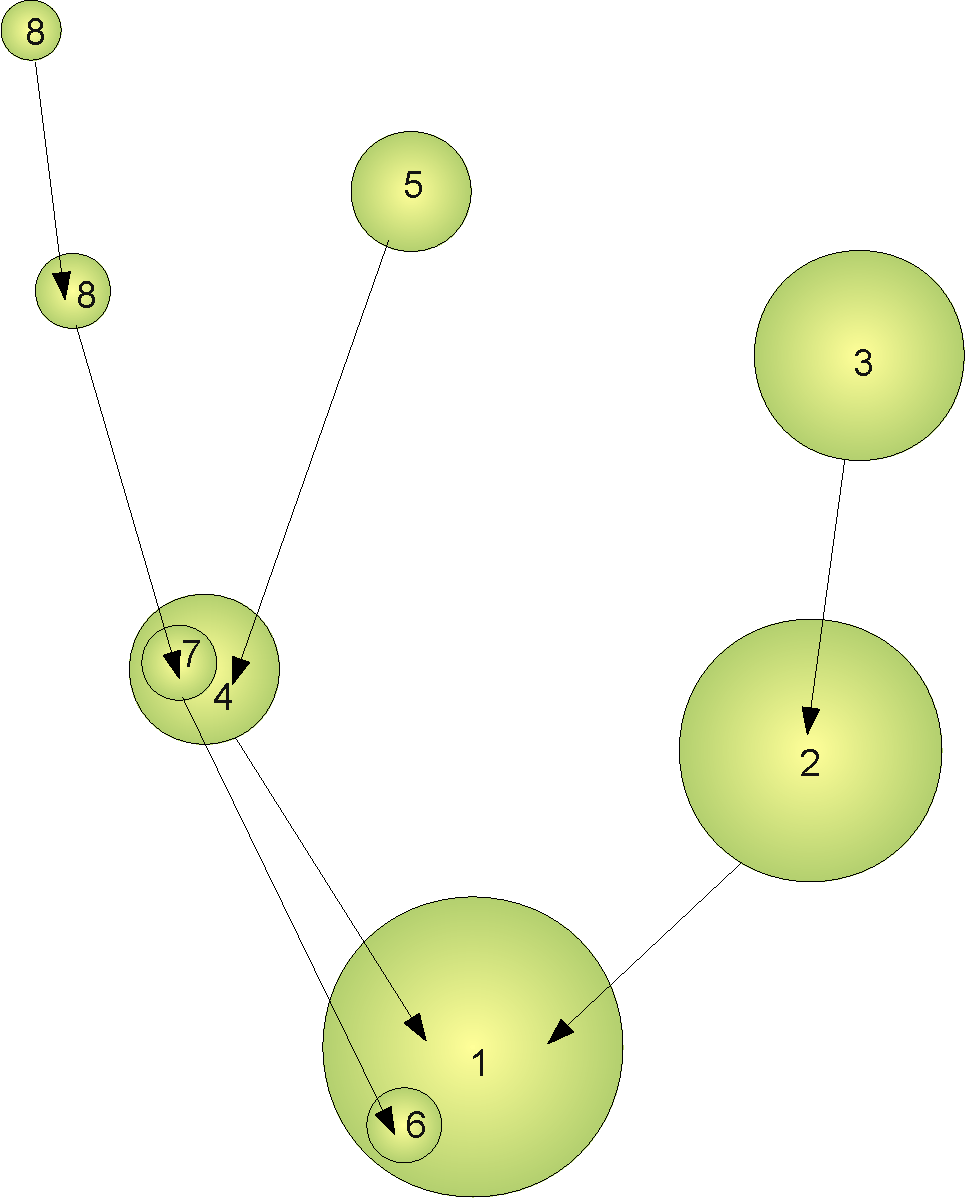
\includegraphics[width=160mm]{Diagrams/MergerTreeSimple.pdf}
 \end{center}
 \caption{An example of a simple merger tree structure. Colored circles represent nodes in the merger tree. Each node has a unique index indicated by the number inside each circle. Black arrows link each node to its descendent node (as specified by the {\normalfont \ttfamily descendentNode} property. Where a node is not its own host node it is placed inside its host node.}
 \label{fig:MergerTreeSimple}
\end{figure}

The following should be noted when constructing merger tree files:
\begin{itemize}
\item Note that \glc\ does not require that nodes be placed on a uniform grid of times/redshifts, nor that mass be conserved along a branch of the tree. After processing the tree in this way, \glc\ builds additional links which identify the child node of each halo and any sibling nodes. These are not required to specify the tree structure but are computationally convenient.
\item It is acceptable for a node to begin its existence as a subhalo (i.e. to have never had an isolated node progenitor). Such nodes will be created as satellites in the merger tree and, providing the selected node components (see \S\ref{sec:Components}) initialize their properties appropriately, will be evolved correctly.
\item It is acceptable for an isolated node to have progenitors, none of which are a primary progenitor. This can happen if all progenitors descend into subhalos in the isolated node. In such cases, \glc\ will create a clone of the isolated node at a very slightly earlier time to act as the primary progenitor. This is necessary to allow the tree to be processed correctly, but does not affect the evolution of the tree.
\item Normally, cases where a node's host node cannot be found in the \gls{forest} will cause \glc\ to exit with an error. Setting {\normalfont \ttfamily [mergerTreeReadMissingHostsAreFatal]}$=${\normalfont \ttfamily false} will instead circumvent this issue by making any such nodes self-hosting (i.e. they become isolated nodes rather than subhalos). Note that this behavior is not a physically correct way to treat such cases---it is intended only to allow trees to be processed in cases where the full \gls{forest} is not available.
\item It is acceptable for nodes to jump between branches in a tree, or even to jump between branches in different trees. In the latter case, all trees linked by jumping nodes (a so-called ``\gls{forest}'' of connected trees) must be stored as a single forest (with multiple root-nodes) in the merger tree file. \glc\ will process this \gls{forest} of trees simultaneously, allowing to nodes to move between their branches.
\item It is acceptable for a subhalo to later become an isolated halo (as can happen due to three-body interactions; see  \citealt{sales_cosmic_2007}). If {\normalfont \ttfamily [mergerTreeReadAllowSubhaloPromotions]}$=${\normalfont \ttfamily true} then such cases will be handled correctly (i.e. the subhalo will be promoted back to being an isolated halo). If {\normalfont \ttfamily [mergerTreeReadAllowSubhaloPromotions]}$=${\normalfont \ttfamily false} then subhalos are not permitted to become isolated halos. In this case, the following logic will be applied to remove all such cases from the tree:\\

\noindent\hspace{ 5mm} $\rightarrow$ \parbox[t]{150mm}{For any branch in a tree which at some point is a subhalo:}\\

\noindent\hspace{10mm} $\rightarrow$ \parbox[t]{145mm}{Beginning from the earliest node in the branch that is a subhalo, repeatedly step to the next descendent node;}\\

\noindent\hspace{10mm} $\rightarrow$ \parbox[t]{145mm}{If that descendent is \emph{not} a subhalo then:}\\

\noindent\hspace{15mm} $\rightarrow$ \parbox[t]{140mm}{If there is not currently any non-subhalo node which has the present node as its descendent then current node is only descendent of a subhalo. Therefore, try to make this node a subhalo, and propose the descendent of the host node of the previous node visited in the branch as the new host:}\\

\noindent\hspace{20mm} $\rightarrow$ \parbox[t]{135mm}{If the proposed host exists:}\\

\noindent\hspace{25mm} $\rightarrow$ \parbox[t]{130mm}{If the mass of the current node is less than that of the proposed host:}\\

\noindent\hspace{30mm} $\rightarrow$ \parbox[t]{125mm}{If the proposed hosts exists before the current node, repeatedly step to its descendents until one is found which exists at or after the time of the current node. This is the new proposed host.}\\

\noindent\hspace{30mm} $\rightarrow$ \parbox[t]{125mm}{If the proposed host is a subhalo, make it an isolated node.}\\

\noindent\hspace{30mm} $\rightarrow$ \parbox[t]{125mm}{The current node is made a subhalo within the proposed host.}\\

\noindent\hspace{25mm} $\rightarrow$ \parbox[t]{130mm}{Otherwise:}\\

\noindent\hspace{30mm} $\rightarrow$ \parbox[t]{125mm}{The current node remains an isolated node, while the proposed host is instead made a subhalo within the current node.}\\

\noindent\hspace{20mm} $\rightarrow$ \parbox[t]{135mm}{Otherwise:}\\

\noindent\hspace{25mm} $\rightarrow$ \parbox[t]{130mm}{The proposed host does not exists, which implies the end of a branch has been reached. Therefore, flag the current node as being a subhalo with a host identical to that of the node from which it descended.}\\
\end{itemize}

\subsubsection{Requirements for \glc\ Input Parameters}

The following requirements must be met for the input parameters to \glc\ when using merger trees read from file:
\begin{itemize}
 \item The cosmological parameters ($\Omega_{\mathrm M}$, $\Omega_\Lambda$, $\Omega_{\mathrm b}$, $H_0$, $\sigma_8$), if defined in the file, must be set identically in the \glc\ input file unless you set {\normalfont \ttfamily [mergerTreeReadMismatchIsFatal]}$=${\normalfont \ttfamily false} in which case you'll just be warned about any mismatch;
 \item \glc\ assumes by default that all merger trees exist at the final output time---if this is not the case set {\normalfont \ttfamily [allTreesExistAtFinalTime]}$=${\normalfont \ttfamily false}.
\end{itemize}

\subsection{Setting of Halo Properties}

\subsubsection{Dark Matter Scale Radii}\index{dark matter halo!concentration}\index{dark matter halo!scale radius}

If {\normalfont \ttfamily [mergerTreeReadPresetScaleRadii]}$=${\normalfont \ttfamily true} and the {\normalfont \ttfamily halfMassRadius} dataset is available within the {\normalfont \ttfamily haloTrees} group (see \S\ref{sec:HaloTreesGroup}) then the half-mass radii of nodes will be used to compute the corresponding scale length of the dark matter halo profile\footnote{The scale radius is found by seeking a value which gives the correct half mass radius. It is therefore important that the definition of halo mass (specifically the virial overdensity) in \protect\glc\ be the same as was used in computing the input half mass radii.}. This requires a dark matter profile scale component which supports setting of the scale length (see \S\ref{sec:DarkMatterProfileComponent}).

\subsubsection{Satellite Merger Times}\index{merger times}\index{satellite!merger times}

If {\normalfont \ttfamily [mergerTreeReadPresetMergerTimes]}$=${\normalfont \ttfamily true} then merger times for satellites will be computed directly from the merger tree data read from file. When a subhalo has an isolated halo as a descendent it is assumed to undergo a merger with that isolated halo at that time. Note that this requires a satellite orbit component method which supports setting of merger times (e.g. {\normalfont \ttfamily [treeNodeMethodSatelliteOrbit]}$=${\normalfont \ttfamily preset}).

\subsubsection{Dark Matter Halo Spins}\index{dark matter halo!spin}

If {\normalfont \ttfamily [mergerTreeReadPresetSpins]}$=${\normalfont \ttfamily true} and the {\normalfont \ttfamily angularMomentum} dataset is available within the {\normalfont \ttfamily haloTrees} group (see \S\ref{sec:HaloTreesGroup}) then the spin parameters of nodes will be computed and set. This requires a dark matter halo spin component which supports setting of the spin (see \S\ref{sec:DarkMatterHaloSpinComponent}).


\chapter{Tutorials}

This chapter contains step-by-step guides to performing common tasks with \glc.

\section{Running \glc\ on N-body Merger Trees}\label{sec:nBodyRun}\index{merger trees!N-body}\index{N-body!merger trees}

See \S\ref{sec:MergerTreeBuilder} for details of how to build merger tree files suitable for input into \glc. There are many options which control precisely how merger trees read from file should be handled. The following section provides guidance on the best choice of parameters.

\subsection{Setting Input Parameters}

To utilize merger trees from the file\footnote{The following assumes that merger trees will be read from a file following \protect\glc's standard HDF5 format which is described in Appendix~\protect\ref{sec:MergerTreeFileFormat}.} that you created in a \glc\ run it's necessary to set two parameters in the input parameter file that you will use for the run:
\begin{verbatim}
  <!-- Specify that merger trees are to be read from file, and give the name of the file to read -->
  <mergerTreeConstructMethod value="read"             />
  <mergerTreeReadFileName    value="myNBodyTrees.hdf5"/>
\end{verbatim}
The first of these {\normalfont \ttfamily [mergerTreeConstructMethod]}$=${\normalfont \ttfamily read} tells \glc\ that merger trees will be constructed by reading them from a file. The second, {\normalfont \ttfamily [mergerTreeReadFileName]}, gives the name of the file from which to read the trees.

In order to choose sensible settings for the various parameters that control merger trees read from file, it is recommended that you read through each of the items below and follow the guidance given.

{\normalfont \bfseries Cosmology:} In addition to specifying that trees should be read from a file, it's also important to ensure that the values of cosmological parameters in \glc\ match those in the merger tree file. (If they don't match, \glc\ will stop with an error message unless you set {\normalfont \ttfamily [mergerTreeReadMismatchIsFatal]}$=${\normalfont \ttfamily false} in which case you'll just be warned about any mismatch.) In our case of using merger trees from the Millennium Simulation, the correct cosmological parameter values can be set as follows:
\begin{verbatim}
  <!-- Use Millennium Simulation cosmology. -->
  <cosmologyParametersMethod value="simple"/>
   <HubbleConstant  value="73.0"  />
   <OmegaMatter     value="0.25"  />
   <OmegaDarkEnergy value="0.75"  />
   <OmegaBaryon     value="0.0455"/>
  </cosmologyParametersMethod>
  <cosmologicalMassVarianceMethod value="filteredPower">
    <sigma_8 value="0.900"/>
  </cosmologicalMassVarianceMethod>
  <powerSpectrumPrimordialMethod value="powerLaw">
    <index               value="1.000"/>
    <wavenumberReference value="1.000"/>
    <running              value="0.000"/>
  </powerSpectrumPrimordialMethod>
\end{verbatim}

{\normalfont \bfseries Existance at Final Time:} Normally, \glc\ assumes that all merger trees will exist (i.e. have at least one node present) at the final output time. This may not be true of trees extracted from an N-body simulation---in this case \glc\ can be informed of this fact by setting:
\begin{verbatim}
  <allTreesExistAtFinalTime value="false"/>
\end{verbatim}

{\normalfont \bfseries Snapping Nodes to Snapshots:} N-body merger trees are often built from ``snapshots'' of the simulation, i.e. all of the nodes exist at a set of discrete times. Often we want to output nodes at precisely these output times. In such cases it is useful to set:
\begin{verbatim}
  <mergerTreeReadOutputTimeSnapTolerance value="1.0d-3"/>
\end{verbatim}
which ensures that the times of nodes are adjusted to lie at precisely the output time if that time is within the specified relative tolerance (this avoids any small differences between node times and output times that can arises due to rounding errors when converting from redshifts to times and vice-versa).

{\normalfont \bfseries Missing Hosts:} \glc\ expects to find each \gls{node}'s host \gls{node} present in a merger tree \gls{forest}. If a \gls{node}'s host is not found this is cause for a fatal error to be issued, since it is impossible to correctly construct and evolve the corresponding \gls{forest}. If you absolutely want to run a \gls{forest} for which one or more host \glspl{node} are missing, you can allow this by setting {\normalfont \ttfamily [mergerTreeReadMissingHostsAreFatal]}$=${\normalfont \ttfamily false}---in this case missing host \glspl{node} trigger a warning only and \glspl{node} without a host are forced to become isolated \glspl{node}. This will lead to incorrect tree evolution however, so the recommended setting is:
\begin{verbatim}
<mergerTreeReadMissingHostsAreFatal value="true"/>
\end{verbatim}

{\normalfont \bfseries Branch Jumps and Subhalo Promotions:} If your merger trees contain subhalos they will most likely exhibit two specific behaviors\footnote{These two behaviors are called out as they specifically \emph{do not} occur in merger trees created using Press-Schechter-based algorithms for example.}: i) \glspl{node} which are subhalos in one timestep may become non-subhalos (isolated halos) in a subsequent timestep (``subhalo promotion''), and ii) \glspl{node} which are subhalos in one branch of the tree may ``jump'' to another branch\footnote{That is, the subhalo's descendented is hosted by a \gls{node} other than the descendent of the subhalo's host.} of the tree becoming a subhalo there (``branch jumping''). These behaviors are fully supported by \glc\ and so we recommend the following settings:
\begin{verbatim}
<mergerTreeReadAllowSubhaloPromotions value="true"/>
<mergerTreeReadAllowBranchJumps       value="true"/>
\end{verbatim}
You may choose to disallow these behaviors by setting either of the above parameters to {\normalfont \ttfamily false}---for example if you wish to explore how your results would differ if subhalos were forced to remain subhalos forever in their original branch. Note that allowing subhalo promotion while not allowing branch jumping can lead to \glspl{deadlock} in merger tree evolution, so change these settings with caution.

Note that for trees which do not contain subhalos these two parameters are irrelevant.

{\normalfont \bfseries Subhalo Masses:} If your trees contain subhalos, the mass evolution of those subhalos can be preset in the satellite component of each \gls{node}. In this way, the subhalo mass in \glc\ will track that specified by the merger tree file. This requires the use of a satellite component which allows presetting of subhalo masses. Recommended settings are therefore:
\begin{verbatim}
<treeNodeMethodSatellite           value="preset"/>
<mergerTreeReadPresetSubhaloMasses value="true"  />
\end{verbatim}
If your trees do not contain subhalos, recommended settings are instead:
\begin{verbatim}
<treeNodeMethodSatellite           value="standard"/>
<mergerTreeReadPresetSubhaloMasses value="false"   />
\end{verbatim}

{\normalfont \bfseries Halo Positions/Velocities:} If your trees contain position and velocity information for halos, those positions and velocities can be preset in the position component of each \gls{node}. This requires the use of a position component which allows presetting of positions and velocities. Recommended settings are therefore:
\begin{verbatim}
<treeNodeMethodPosition        value="preset"/>
<mergerTreeReadPresetPositions value="true"  />
\end{verbatim}
If your trees do not contain position information recommended settings are:
\begin{verbatim}
<treeNodeMethodPosition        value="null" />
<mergerTreeReadPresetPositions value="false"/>
\end{verbatim}

{\normalfont \bfseries Subhalo Orbits:} If your trees contain position and velocity information they can be used to preset initial orbit information for subhalos. Note that it is not required that your trees contain subhalos for this orbit presetting to be performed---\glc\ can follow subhalo orbits even if subhalos are not included in the trees themselves. The following settings are recommended:
\begin{verbatim}
<mergerTreeReadPresetOrbits             value="true"/>
<mergerTreeReadPresetOrbitsSetAll       value="true"/>
<mergerTreeReadPresetOrbitsAssertAllSet value="true"/>
<mergerTreeReadPresetOrbitsBoundOnly    value="true"/>
\end{verbatim}
These options will cause an orbit to be preset for each subhalo based on the relative position and velocity of merging halos and assuming that the orbital energy and angular momentum are conserved between the time immediately prior to the merger and the time of virial radius crossing. If the computed orbit does not cross the virial radius of the larger halo or if the computed orbit is unbound, the above options cause an orbit to be preset by drawing orbital parameters at random from the chosen cosmological distribution (see \S\ref{sec:SatelliteVirialOrbits}).

{\normalfont \bfseries Subhalo Merging:} If your merger trees contain subhalo information, that information can be used to specify when, and with which other node, each subhalo merges. Specifically, a subhalo is assumed to merge at the time at which it is not the primary progenitor of its descendent halo---possibly with some other delay to be described below. Recommended settings are:
\begin{verbatim}
<mergerTreeReadPresetMergerTimes          value="true"             />
<mergerTreeReadPresetMergerNodes          value="true"             />
<mergerTreeReadSubresolutionMergingMethod value="boylanKolchin2008"/>
\end{verbatim}
The first two options cause subhalos to merge at the time described above, and with their descendent node. The final option accounts for the possibility that the subhalo should not actually merge immediately at this time. For example, in N-body simulations, the subhalo may have simply been lost due to limitations of resolution or halo finder algorithms. The final option specifies that some additional time until merging be added based on the subhalo merging timescale algorithm of \citeauthor{boylan-kolchin_dynamical_2008}~[\citeyear{boylan-kolchin_dynamical_2008}; see \S\ref{phys:satelliteMergingTimescales:satelliteMergingTimescalesBoylanKolchin2008}], and computed using the last known orbital properties of the subhalo.

{\normalfont \bfseries Halo Scale Radii:} If your merger trees contain information on halo scale radii or half-mass radii, these can be used to preset the scale radius of each \gls{node}. This requires the use of a dark matter profile component which allows presetting of scale length. Recommended settings are therefore:
\begin{verbatim}
<mergerTreeReadPresetScaleRadii                     value="true"     />
<mergerTreeReadPresetScaleRadiiFailureIsFatal       value="true"     />
<mergerTreeReadPresetScaleRadiiConcentrationMinimum value="3"        />
<mergerTreeReadPresetScaleRadiiConcentrationMaximum value="60"       />
<mergerTreeReadPresetScaleRadiiMinimumMass          value="see below"/>
\end{verbatim}
Minimum and maximum concentrations are specified---these are used to restrict the range of scale radii that are allowed for a given halo. If scale radii are to be determined based on half-mass radii given in the merger tree file, and if the computed scale radius does not result in a concentration between these limits, then a fatal error is issued.

Finally, you can set a minimum halo mass via the {\normalfont \ttfamily [mergerTreeReadPresetScaleRadiiMinimumMass]} parameter below which the scale radii or half-mass radii in your file should be considered not reliable. For halos below this mass, scale radii will instead be assigned via the selected dark matter halo concentration method (see \S\ref{sec:DarkMatterProfileConcentration}).

{\normalfont \bfseries Halo Angular Momenta:} If your merger trees contain spin or angular momentum information these can be preset for each node. Recommended settings are:
\begin{verbatim}
<treeNodeMethodSpin                  value="preset"/>
<mergerTreeReadPresetSpins           value="true"  />
<mergerTreeReadPresetUnphysicalSpins value="true"  />
\end{verbatim}
The last of these options causes any halos for which the spin given in the merger tree file is non-positive to be assigned a spin at random instead, drawn from the specified cosmological distribution (see \S\ref{sec:SpinParameterDistribution}).

If subhalo masses are not included in their host halo masses in your merger tree file, you should specify how the angular momenta of subhalos should be accounted for when adding their mass to their host halo. If positions and 3D angular momenta are available in your merger tree file, the recommended setting is:
\begin{verbatim}
<mergerTreeReadSubhaloAngularMomentaMethod value="summation"/>
\end{verbatim}
If this information is not present 
\begin{verbatim}
<mergerTreeReadSubhaloAngularMomentaMethod value="scale"    />
\end{verbatim}
should be used instead.

If your merger tree file contains 3D spin or angular momentum information, you can choose to make that information available within \glc\ be using the settings:
\begin{verbatim}
<treeNodeMethodSpin          value="preset3D"/>
<mergerTreeReadPresetSpins3D value="true"    />
\end{verbatim}

{\normalfont \bfseries Subhalo Indices:} If your merger trees contain subhalos, you can tell \glc\ to keep track of the indices of subhalos by setting:
\begin{verbatim}
<treeNodeMethodSatellite            value="preset"/>
<mergerTreeReadPresetSubhaloIndices value="true"  />
\end{verbatim}
The \glc\ output file will then contain {\normalfont \ttfamily satelliteNodeIndex} datasets which list the index (as given in the merger tree file) for all subhalos and halos. Without specifying this presetting, the index of subhalos is frozen at the index of the halo immediately prior to it becomming a subhalo.

The remainder of this section gives more detail about many of the parameters described above and how they affect handling of merger trees read from file. Further parameters can be set to control what information from the stored trees will be used in \glc. Examples are given below.

\subsection{Further Details}

Further details of the effects of the many parameters controlling merger trees read from file are given below.

\subsubsection{Node Positions}

If position and velocity information for tree nodes is available within the merger tree file then \glc\ can be instructed to use this information by using the ``preset'' method for tree node positions and telling the merger tree construction method to preset node positions as follows:
\begin{verbatim}
  <!-- Use merger tree node positions -->
  <treeNodeMethodPosition        value="preset"/>
  <mergerTreeReadPresetPositions value="true"  />
\end{verbatim}
If position information is unavailable, the ``null'' position method can be selected and the merger tree construction method instructed not to preset positions as follows:
\begin{verbatim}
  <!-- Do not use merger tree node positions -->
  <treeNodeMethodPosition        value="null" />
  <mergerTreeReadPresetPositions value="false"/>
\end{verbatim}

\subsubsection{Virial Orbits}\index{orbits!virial}\index{orbits!setting}\index{orbits!N-body}

If position and velocity information for tree nodes is available within the merger tree file then \glc\ can be instructed to use this information to estimate the orbit of each subhalo at the point at which it crosses the virial radius of its host halo. This ``virial orbit'' may then be used by, for example, calculations of merging timescales.
\begin{verbatim}
  <!-- Use merger tree node positions to compute orbits at the virial radius -->
  <mergerTreeReadPresetOrbits             value="true"/>
  <mergerTreeReadPresetOrbitsBoundOnly    value="true"/>
  <mergerTreeReadPresetOrbitsSetAll       value="true"/>
  <mergerTreeReadPresetOrbitsAssertAllSet value="true"/>
\end{verbatim}
Typically, a merging halo is not seen at precisely the time at which it crosses the virial radius of its host (due to the fact that N-body simulations are output at discretely spaced timesteps). Therefore, \glc\ computes the orbit at the time just prior to merging and assumes that the orbital parameters (energy and angular momentum) remain fixed to propagate the orbit to the virial radius of the host. The second parameter in the above example, {\normalfont \ttfamily [mergerTreeReadPresetOrbitsBoundOnly]}, specifies whether or not only bound orbits should be set. Some calculations (e.g. of subhalo merging times) assume bound orbits and may fail if given an unbound orbit. Setting this option to {\normalfont \ttfamily true} causes only bound orbits to be preset---unbound orbits are ignored. Note that some orbits cannot be propagated to the virial radius (i.e. their pericenter is larger than the virial radius). The {\normalfont \ttfamily [mergerTreeReadPresetOrbitsSetAll]} option, if true, will cause such orbits to be assigned randomly using the selected {\normalfont \ttfamily [virialOrbitsMethod]}, such that all orbits are assigned. The {\normalfont \ttfamily [mergerTreeReadPresetOrbitsAssertAllSet]} option requires that all orbits be set---if {\normalfont \ttfamily [mergerTreeReadPresetOrbitsSetAll]}$=${\normalfont \ttfamily false} and {\normalfont \ttfamily [mergerTreeReadPresetOrbitsAssertAllSet]}$=${\normalfont \ttfamily true} then \glc\ will exit with an error message if any orbit cannot be set.

If the satellite component additionally permits setting of the satellite position and velocity, these properties will also be assigned based on the relative position and velocity of the satellite and host halos.

\subsubsection{Merging Times and Targets}

The times at which subhalos merge with their host halo can be determined directly from the merger tree file if subhalo information is included in that file. Merging is assumed to occur when the subhalo no longer has a distinct descendent (i.e. it descends into a non-subhalo). If merging times are to be computed in this way set
\begin{verbatim}
  <treeNodeMethodSatellite         value="preset"/>
  <mergerTreeReadPresetMergerTimes value="true"  />
\end{verbatim}
which select a satellite orbit method that allows merger times to be present and tell the merger tree construction method to preset those merger times respectively. If merger times are not to be computed in this way then instead set, for example,
\begin{verbatim}
  <treeNodeMethodSatellite         value="standard" />
  <mergerTreeReadPresetMergerNodes value="false"    />
  <satelliteMergingMethod          value="Jiang2008"/>
\end{verbatim}
which selects a standard satellite orbit method, prevents attempts to preset the merger times and selects the {\normalfont \ttfamily Jiang2008} method for computing merger times instead.

In addition to setting the times of merger events, it is possible to set the target node with which a merging node should merge. By default, \glc\ will assume that all merging occurs with the non-subhalo host node in which a subhalo is located. This may not be the desired behavior when using N-body merger trees. For example, such trees may indicate that a subhalo merges with another subhalo. Setting
\begin{verbatim}
  <mergerTreeReadPresetMergerNodes value="true"/>
\end{verbatim}
will cause the target node with which each merger should occur to be determined from the merger tree structure and preset for use in \glc.

It is possible to add a delay between the last time at which a subhalo was seen in a simulation and the time at which it is considered to merge. This functionality is motivated by the consideration that a subhalo vanishing from a simulation may be simply due to it dropping below resolution rather than it actually having undergone a merger. The parameter {\normalfont \ttfamily [mergerTreeReadSubresolutionMergingMethod]} can be used to select a satellite merging timescale method (see \S\ref{sec:SatelliteMergingTimescales}) to use in this case. (It is set by default to ``{\normalfont \ttfamily null}'' such that no delay before merging occurs.) The orbit of the subhalo around its parent at the last time it is present in the merger tree is passed to this method and used to estimate a time until merging. This delay is added to the time at which the subhalo merges and, if merge target nodes are being set, the target node is updated accordingly.

\subsubsection{Subhalo Indices}

The indices of subhalos are usually frozen at the index of the halo just prior to becoming a subhalo. The index of the corresponding halo in the original tree (as read from file) can be tracked as follows:
\begin{verbatim}
  <treeNodeMethodSatellite            value="preset"/>
  <mergerTreeReadPresetSubhaloIndices value="true"  />
\end{verbatim}
to first select the ``preset'' satellite orbit method (which allows subhalo indices to be preset) and, second, to instruct the merger tree construction algorithm to preset those indices. The index will then be available in output as {\normalfont \ttfamily satelliteNodeIndex}.

\subsubsection{Subhalo Masses}

The masses of subhalos (specifically their time evolution after they become subhalos) can be set using the values stored in the merger tree file (if available). To set subhalo masses in this way use
\begin{verbatim}
  <treeNodeMethodSatellite           value="preset"/>
  <mergerTreeReadPresetSubhaloMasses value="true"  />
\end{verbatim}
to first select the ``preset'' satellite orbit method (which allows subhalo masses to be preset) and, second, to instruct the merger tree construction algorithm to preset those masses.

\subsubsection{Node Spins}

If information on the angular momenta of nodes is available in the merger tree file, this can be used to preset the value of the spin parameter in each node\footnote{Before doing this, it is important to be sure that the angular momenta of the nodes are reliable. For example, in low mass nodes extracted from an N-body simulation resolution effect may limit the accuracy of the measured angular momentum.} by setting:

\begin{verbatim}
  <mergerTreeReadPresetSpins value="true"/>
\end{verbatim}

The spin parameter is set using the spin of each node if available, or otherwise using the angular momentum of each node stored in the merger tree file using:
\begin{equation}
 \lambda = {|\mathbf{J}| |E|^{1/2} \over \mathrm{G} M^{5/2}}
\end{equation}
where $|\mathbf{J}|$ is the magnitude of the node's angular momentum, $M$ is the node's mass and $E$ is its energy. Additionally, by setting:

\begin{verbatim}
  <mergerTreeReadPresetSpins3D value="true"/>
\end{verbatim}
the spin vector of each node will be set (assuming that the vector spin or angular momenta of nodes are available in the merger tree file) using:
\begin{equation}
 \mathbf{\lambda} = {\mathbf{J} |E|^{1/2} \over \mathrm{G} M^{5/2}}.
\end{equation}

If spins could not be determined for some halos the spin (or angular momentum) should be set to zero in the merger tree file, and the parameter {\normalfont \ttfamily [mergerTreeReadPresetUnphysicalSpins]} set to {\normalfont \ttfamily true}. \glc\ will then assign a spin to such halos by sampling from the selected spin distribution (see \S\ref{sec:SpinParameterDistribution}). 

\subsubsection{Node Scale Radii}

If information on the half-mass or scale radii of nodes is available in the merger tree file, it can be used to preset the value of the dark matter halo scale radius in each node by setting:

\begin{verbatim}
  <mergerTreeReadPresetScaleRadii value="true"/>
\end{verbatim}

Before doing this, it is important to be sure that the half-mass or scale radii of the nodes are reliable. For example, in low mass nodes extracted from an N-body simulation resolution effect may limit the accuracy of the measured half-mass or scale radius. In such cases, use the {\normalfont \ttfamily [mergerTreeReadPresetScaleRadiiMinimumMass]} parameter to specify the lowest mass halos for which the scale radii should be preset---lower mass halos will be assigned a scale radius using the method specified by the {\normalfont \ttfamily [mergerTreeReadConcentrationFallbackMethod]} parameter (which will default to the value of {\normalfont \ttfamily [darkMatterConcentrationMethod]}; see \S\ref{sec:DarkMatterProfileConcentration}). It is also possible to specify minimum and maximum allowed concentrations when computing the scale radius from the half mass radius using the {\normalfont \ttfamily [mergerTreeReadPresetScaleRadiiConcentrationMinimum]} and {\normalfont \ttfamily [mergerTreeReadPresetScaleRadiiConcentrationMaximum]} parameters. If matching the half mass radius would require a concentration outside of this range, \glc\ will abort unless {\normalfont \ttfamily [mergerTreeReadPresetScaleRadiiFailureIsFatal]}$=${\normalfont \ttfamily false}, in which case it will instead silently use the fallback concentration method described above.

If only half-mass radii are available, the scale radius is set by using a root finding algorithm to ensure that half of the total halo mass is enclosed within the specified half-mass radius.

\subsubsection{Miscellaneous N-body Properties}

Several miscellaneous properties often available from N-body merger trees can also be preset by setting the following parameters to {\normalfont \ttfamily true}:
\begin{description}
\item[{mergerTreeReadPresetParticleCounts}] Sets the number of particles in each halo (requires the {\normalfont \ttfamily particleCount} dataset to be present in the merger tree file);
\item[{mergerTreeReadPresetVelocityMaxima}] Sets the maxima of halo rotation curves (requires the {\normalfont \ttfamily velocityMaximum} dataset to be present in the merger tree file);
\item[{mergerTreeReadPresetVelocityDispersions}] Sets the velocity dispersion of halos (requires the {\normalfont \ttfamily velocityDispersion} dataset to be present in the merger tree file).
\end{description}

\subsubsection{Subhalo Promotion}\label{sec:Tutorial:NbodyTrees:SubhaloPromotion}

A subhalo may, at a later time, become an isolated halo once again. \glc\ allows you to control whether such behavior is allowed, or should be prohibited. To allow such ``subhalo promotion'', set:
\begin{verbatim}
<mergerTreeReadAllowSubhaloPromotions value="true"/>
\end{verbatim}
If you choose to inhibit this behavior by setting the above parameter to false, a halo that becomes a subhalo will remain a subhalo forever thereafter. Note that the isolated halo to which it would have been promoted will still exist, and may therefore form its own galaxy. This can result in double counting of mass, and so inhibiting subhalo promotion is not recommended.

\subsubsection{``Fly-by'' Halos}\label{sec:Tutorial:NbodyTrees:BranchJump}

In some cases, a halo that is part of one tree can later become part of another tree. This can happen in so-called ``fly-by'' encounters where a halo may briefly become a subhalo in a halo in tree A then leave that halo and become a subhalo in tree B.

The correct way to handle this issue is to combine trees A and B into a single tree (which will now have multiple base nodes). \glc\ will then process these two trees simultaneously, correctly handling the fly-by, and outputting the trees as two separate trees.

If for some reason this is not possible or desired, the fly-by problem will normally cause \glc\ to complain that the host halo of a node cannot be found (since it exists in a different tree). This problem can be avoided by setting:
\begin{verbatim}
  <mergerTreeReadMissingHostsAreFatal value="false"/>
\end{verbatim}
In this case, nodes with missing hosts are simply treated as being isolated halos. This will avoid an error condition, but is not a physically correct way to handle such cases, so use with caution.

\subsection{Using Particles to Track Unresolved Subhalos}

In N-body simulations it is possible that a subhalo can become ``lost'' from the simulation (i.e. can no longer be identified by a halo finder due to resolution issues) before it has actually merged with the central galaxy or been completely tidally destroyed. In such cases it is useful to be able to assign a position to the subhalo at later times. A common approach to assigning a position (and velocity) is to use that of the most bound particle in the subhalo at the last time it was identified. \glc\ allows for particle tracking in this way through the addition of particle information to the merger tree file.

To add particle tracking data to a merger tree file, follow these steps:
\begin{enumerate}
\item Identify all subhalos which are lost from the simulation prior to the final timestep;
\item Determine the index of the most bound particle in each such subhalo in the last timestep in which it was identified;
\item For each subhalo, extract the redshift, position, and velocity of that particle (which is usally trivial to do once its index is known) at each subsequent timestep in the simulation;
\item Write these data (along with the particle index) to the {\normalfont \ttfamily particles} group in the merger tree file as described in \S\ref{sec:MergerTreeFormatDescription:Particles};
\item Add two datasets to the {\normalfont \ttfamily forestHalos} group:
  \begin{enumerate}
  \item {\normalfont \ttfamily particleIndexStart} which should indicate the index in the datasets in the {\normalfont \ttfamily particles} group at which the data for each halo begins (or $-1$ if no particle data is included for the halo);
  \item {\normalfont \ttfamily particleIndexCount} which should indicate the number of entries in the datasets in the {\normalfont \ttfamily particles} group for each halo (or $-0$ if no particle data is included for the halo).
  \end{enumerate}
\end{enumerate}

\subsection{Handling of Extremely Large Merger Tree Forests}\index{merger trees!large}\index{forests!large}

Halos can move between merger trees (see \S\ref{sec:Tutorial:NbodyTrees:SubhaloPromotion} and \S\ref{sec:Tutorial:NbodyTrees:BranchJump}), leading to the necessity of merger tree forests---interconnected groups of merger trees that \glc\ typically processes as a whole. These forests can become very large---in some cases so large that they do not fit within the available memory. \glc\ can handle such forests by splitting them into individual trees. Each tree is processed separately, and nodes are moved between trees as needed. If a tree needs a node from another tree before its evolution can continue, its state can be suspended to disk, and later re-read once the node it requires becomes available. In this way, very large forests can be processed without running out of memory (as trees are stored to disk while they are not being processed).

To cause forests to be split in this way, the following parameters should be set:
\begin{verbatim}
  <treeEvolveSuspendToRAM                   value="false"            />
  <treeEvolveSuspendPath                    value="/my/scratch/path/"/>
  <mergerTreeReadForestSizeMaximum          value="10000000"         />
  <mergerTreeReadSubresolutionMergingMethod value="infinite"         />
\end{verbatim}

Here, {\normalfont \ttfamily treeEvolveSuspendToRAM} specifies that merger trees should be suspended to disk (i.e. not to RAM which is the default), and {\normalfont \ttfamily treeEvolveSuspendPath} gives a path where the suspended trees can be written---typically scratch space local to the compute node where \glc\ is being run is a good option.
 
{\normalfont \ttfamily mergerTreeReadForestSizeMaximum} specifies the maximum number of nodes allowed in a forest before it will be split. A suitable number for this depends on the details of the available RAM, the number of threads sharing that RAM, and the characteristics of the \glc\ model being used (which will affect the memory required per node).
 
Finally, {\normalfont \ttfamily mergerTreeReadSubresolutionMergingMethod} is set to {\normalfont \ttfamily infinite} to prevent any merging (which is not supported for split forests at present, although it should be soon).

\subsection{Analyzing the Output}

\subsubsection{Positions and Velocities}

Components of the position of each node are output as {\normalfont \ttfamily positionX}, {\normalfont \ttfamily positionY} and {\normalfont \ttfamily positionZ} and can be accessed in the same way as other output properties from \glc\ (see \S\ref{sec:nodeDataGroup}).

\subsubsection{Subhalo Masses}

The current mass of subhalos is available via the {\normalfont \ttfamily nodeBoundMass} output dataset and can be accessed in the same way as other output properties from \glc\ (see \S\ref{sec:nodeDataGroup}). For non-subhalos this property is equal to the usual {\normalfont \ttfamily nodeMass} property.

\section{Generating Mock Catalogs with Lightcones from the Millennium Simulation}\index{lightcone}\index{Millennium Simulation}\index{mock catalog}

Suppose that you want to create a catalog of galaxies as would be found in a survey of an area of the sky out to some redshift. Such a ``mock catalog'' can be built by populating with galaxies all of the dark matter halos which happen to lie within the cone which that area makes as it is projected from the observer through the Universe.

Generating such a mock catalog using \glc\ involves first extracting the halos (and their merger trees) within this ``lightcone'' from a suitable N-body simulation, and then processing them through \glc. In this tutorial, we will specifically make use of the \href{http://gavo.mpa-garching.mpg.de/MyMillennium3/MyDB}{Millennium Simulation database} to provide the merger trees, but the same principles apply to any N-body simulation.

The script, {\normalfont \ttfamily scripts/aux/Millennium\_Lightcone\_Grab.pl} can be used to retrieve merger trees that intersect a given lightcone from the Millennium Database and to store them in \glc's format (see \S\ref{sec:MergerTreeFileFormat}). The script is used as follows:
\begin{verbatim}
scripts/aux/Millennium_Lightcone_Grab.pl <lightconeDirectory> <fieldSize> <maximumRedshift>
    --user <myUserName> --password <myPassword> --treesPerFile <treesPerFile>
\end{verbatim}
Here, {\normalfont \ttfamily \textless lightconeDirectory\textgreater} is the name of a (pre-existing) directory into which merger tree data will be stored, {\normalfont \ttfamily \textless fieldSize\textgreater} is the length (in degrees) of one side of the square field of view of the lightcone, {\normalfont \ttfamily \textless maximumRedshift\textgreater} is the highist redshift for which halos should be included in the catalog. The {\normalfont \ttfamily --user} and {\normalfont \ttfamily --password} options allow you to specify your username and password for accessing the Millennium Simulation database. Finally, the {\normalfont \ttfamily --treesPerFile} specifies how many merger trees should be stored in each file (the script will split the lightcone between many files---this is primarily so that each request sent to the Millennium Database server is not too large). If no value is specified a default of 200 trees per file will be used.

The script generates multiple SQL queries to the Millennium database in order to first find all halos which intersect the lightcone and second to retrieve the complete merger tree associated with each such halo. These merger trees are then stored in \glc's merger tree file format in files named {\normalfont \ttfamily Lightcone\_Trees\_AAA:BBB.hdf5} in the given {\normalfont \ttfamily \textless lightconeDirectory\textgreater}, where {\normalfont \ttfamily AAA} and {\normalfont \ttfamily BBB} are numbers giving the first and last trees in the file\footnote{Note that these are not the ID numbers of the trees, just a sequential count of all trees retrieved.}

Each of the merger tree files created can then be run through \glc\ in the usual way (see \S\ref{sec:nBodyRun}).  Outputs should be requested at every Millennium snapshot (up to the largest redshift to be considered), and the {\normalfont \ttfamily lightcone} filter should be used to cause only those galaxies which intersect the lightcone to be output---for example:
\begin{verbatim}
<!-- Set output redshifts to the snapshots in the milliMillennium. -->
<outputRedshifts value=
   "0.0000 0.0199 0.0414 0.0645 0.0893 0.1159 0.1444 0.1749 0.2075 0.2425
    0.2798 0.3197 0.3623 0.4079 0.4566 0.5086 0.5642 0.6236 0.6871 0.7550
    0.8277 0.9055 0.9887 1.0779 1.1734 1.2758 1.3857 1.5036 1.6303 1.7663
    1.9126 2.0700 2.2395 2.4220 2.6189 2.8312 3.0604 3.3081 3.5759 3.8657
    4.1795 4.5196 4.8884 5.2888 5.7239 6.1968"
/>

<!-- Add a lightcone filter with the required geometry -->
<mergerTreeOutput>
  <galacticFilterMethod value="lightcone"/>
</mergerTreeOutput>

<!-- Switch on output of lightcone data -->
<outputLightconeData value="true"/>

<!-- Prune away trees not appearing in the lightcone -->
<mergerTreeOperatorMethod value="pruneLightcone"/>

<!-- Specify lightcone geometry -->
<geometryLightconeMethod value="square">
  <origin value="0 0 0"/>
  <unitVector1 value=" 1 1  1"/>
  <unitVector2 value=" 0 1 -1"/>
  <unitVector3 value="-2 1  1"/>
  <lengthReplication value="500"/>
  <lengthHubbleExponent value="-1"/>
  <lengthUnitsInSI value="3.08567758135e22"/>
  <angularSize value="0.5"/>
  <timeEvolvesAlongLightcone value="true"/>
  <redshift value=
   "0.0000 0.0199 0.0414 0.0645 0.0893 0.1159 0.1444 0.1749 0.2075 0.2425
    0.2798 0.3197 0.3623 0.4079 0.4566 0.5086 0.5642 0.6236 0.6871 0.7550
    0.8277 0.9055 0.9887 1.0779 1.1734 1.2758 1.3857 1.5036 1.6303 1.7663
    1.9126 2.0700 2.2395 2.4220 2.6189 2.8312 3.0604 3.3081 3.5759 3.8657
    4.1795 4.5196 4.8884 5.2888 5.7239 6.1968"
  />
</geometryLightconeMethod>
\end{verbatim}
In the above {\normalfont \ttfamily [outputLightconeData]} causes lightcone coordinate information (i.e. the position and velocity of each galaxy in a coordinate system with axes aligned along the line of sight of the lightcone and parallel to the two edges of the square field of view, along with the redshift) to be output (see \S\ref{sec:OutputLightcone}), and {\normalfont \ttfamily [mergerTreeOperatorMethod]} is set to {\normalfont \ttfamily pruneLightcone} to cause any merger trees which have no nodes within the lightcone volume to be pruned away (as there is no need to process them). Finally, the {\normalfont \ttfamily geometryLightconeMethod} parameter describes the geometry of the lightcone to be used---see \S\ref{sec:methodsGeometryLightcone} for details.

\section{Using the Instantaneous Recycling Approximation}\index{recycling!instantaneous}\index{instantaneous recycling approximation}

Choosing {\normalfont \ttfamily [stellarPopulationPropertiesMethod]}$=${\normalfont \ttfamily instantaneous} will cause \glc\ to use the instantaneous recycling approximation for all calculations of stellar populations. The recyling rate and yield to use are set by the {\normalfont \ttfamily [imfNAMERecycledInstantaneous]} and {\normalfont \ttfamily [imfNAMEYieldInstantaneous]} parameters respectively, where {\normalfont \ttfamily NAME} is the name of the appropriate \gls{imf}.

Setting {\normalfont \ttfamily [stellarPopulationPropertiesMethod]}$=${\normalfont \ttfamily noninstantaneous} causes \glc\ to use a fully non-instantaneous, metal-depdendent calculation of recycling, metal production and \gls{sne} rates. However, it is possible to force this method to operate in the instantaneous recycling approximation limit (which can be useful for testing and comparison) by setting:
\begin{verbatim}
  <!-- Force the calculation of recycling, yields etc. to   -->
  <!-- be done assuming instantaneous recycling             -->
  <starFormationImfInstantaneousApproximation value="true"/>
  <!-- Set the mass of stars which should be used as the    -->
  <!-- dividing line between long-lived and instantaneously -->
  <!-- evolving in this approximation.                      -->
  <starFormationImfInstantaneousApproximationMassLongLived value="1.0"/>
  <!-- Set the effective age of populations to use in this -->
  <!-- approximation when computing SNe numbers.           -->
  <starFormationImfInstantaneousApproximationEffectiveAge value="13.8"/>
\end{verbatim}

\section{Postprocessing of Stellar Spectra}

Stellar luminosities are computed by convolving a library of simple stellar populations with the star formation history of each galaxy. \glc\ allows the spectra of those simple stellar populations to be postprocessed (after being read from file or internally generated for example) before they are utilized in the convolution integral. This postprocessing can modify the spectra in arbitrary ways that depend on wavelength, redshift, and age of stellar population. Furthermore, \glc\ allows you to chain together stellar spectra postprocessors into a set to allow multiple postprocessings to be applied. Furthermore again, you can define an arbitrary number of sets and apply different sets to different luminosities.

Typical uses of stellar spectra postprocessors include accounting for absorption of galaxy light by the intervening \gls{igm}, or capturing only the light from recent star formation\footnote{Perhaps so that additional dust extinction can be applied to the light of recently formed stars.}. A full list of the available postprocessors can be found in \S\ref{sec:StellarSpectraPostprocessing}.

If you don't specify a postprocessing set, the ``default'' set (consisting of the {\normalfont \ttfamily inoue2014} postprocessor; see \S\ref{phys:spectraPostprocessor:spectraPostprocessorInoue2014}) is applied to each luminosity calculation. To specify other postprocessing sets add the following to your parameter file:
\begin{verbatim}
 <luminosityPostprocessSet value="default recent unabsorbed recentUnabsorbed"/>
\end{verbatim}
where one set must be specified for each luminosity specified in the {\normalfont \ttfamily luminosityFilter} parameter. Note that set names can be reused in order to apply the same postprocessor set to multiple luminosities.

The chain of postprocessors to apply for each set is then specified as follows:
\begin{verbatim}
 <stellarPopulationSpectraPostprocessRecentMethods           value="inoue2014 recent"/>
 <stellarPopulationSpectraPostprocessUnabsorbedMethods       value="identity"        />
 <stellarPopulationSpectraPostprocessRecentUnabsorbedMethods value="recent"          />
\end{verbatim}
In this case we've constructed three new sets, in addition to the default set (which applies just the {\normalfont \ttfamily inoue2014} postprocessor). The {\normalfont \ttfamily recent} set applies both the {\normalfont \ttfamily inoue2014} \gls{igm} absorption postprocessor, followed by the {\normalfont \ttfamily recent} postprocessor to retain only recently emitted light. The {\normalfont \ttfamily unabsorbed} set ignores \gls{igm} absorption entirely---it does this by using the {\normalfont \ttfamily identity} postprocessor which leaves the spectrum unaffected. Finally, the {\normalfont \ttfamily recentUnabsorbed} set applies only the {\normalfont \ttfamily recent} filter while ignoring \gls{igm} absorption.

In this way it is relatively easy to extract multiple different measures of luminosity from a \glc\ model. For example, you could construct four postprocessor sets, each corresponding to one of the four different \gls{igm} absorption models ({\normalfont \ttfamily lycSuppress}, {\normalfont \ttfamily madau1995}, {\normalfont \ttfamily meiksin2006}, and {\normalfont \ttfamily inoue2014}) and apply these to the same luminosity filter to assess how luminosity depends on the \gls{igm} model used.

\section{Migrating Parameter Files to a New Version}\label{sec:MigrateParameters}\index{migration}\index{parameters}

The names and allowed values of parameters often change between versions of \glc. To permit easy and error-free migration between versions a script is provided to translate parameter files from earlier to later versions. To migrate a parameter file simply use:
\begin{verbatim}
scripts/aux/parametersMigrate.pl parameters.xml newParameters.xml
\end{verbatim}
By default, this script will translate from the previous to the current version of \glc. If your parameter file contains a {\normalfont \ttfamily version} element then this will be used to determine which version of \glc\ the parameter file was constructed for. The migration script will then migrate the parameter file through all intermediate versions to bring it into compliance with the current version. You can also specify input and output versions directly:
\begin{verbatim}
scripts/aux/parametersMigrate.pl parameters.xml newParameters.xml --inputVersion 0.9.0 --outputVersion 0.9.3
\end{verbatim}
will convert {\normalfont \ttfamily parameters.xml} from version 0.9.0 syntax to version 0.9.3 syntax.

\subsection{Reionization Calculations}\label{sed:ReionziationTutorial}\index{reionization}

\glc\ can self-consistently solve for the evolution of the \gls{igm} as it becomes photoionized by light emitted by stars and AGN. To activate this calculation, include the following in your parameters file:
\begin{verbatim}
  <!-- IGM evolver -->
  <intergalacticMediumStateMethod  value="internal"/>
  <igmPropertiesCompute            value="true"    />
  <igmPropertiesTimeCountPerDecade value="10"      />
  
  <!-- Background radiation -->
  <backgroundRadiationCompute                  value="true"    />
  <radiationIntergalacticBackgroundMethod      value="internal"/>
  <backgroundRadiationWavelengthCountPerDecade value="50"      />
  <backgroundRadiationTimeCountPerDecade       value="10"      />

  <!-- Halo accretion options -->
  <accretionHaloMethod value="naozBarkana2007"/>
\end{verbatim}
The first block of parameters switches \glc\ to using an internal calculation for the state of the \gls{igm}, instructs it to solve for \gls{igm} properties as a function of time, and specifies that \gls{igm} properties should be updated 10 times per decade of cosmic time. Specifically, at each of these time intervals, solving of galaxy evolution is halted and the \gls{igm} evolved up to this time using the currently computed photoionizing background spectrum.

The second block of parameters activates an internal calculation of cosmic background radiation, in which the background is computed from the emissivities of model galaxies and AGN. The number of points at which to tabulate the background per decade of wavelength and cosmic time are specified.

Finally, the third block of parameters tells \glc\ to use the \cite{naoz_formation_2007} prescription for computing gas accretion into halos from the \gls{igm}. This prescription uses the filtering mass to determine accretion rates, and will take the filtering mass from the internal \gls{igm} evolution calculation.

With these three sets of configurations, \glc\ will perform a self-consistent evolution of the \gls{igm}---in the sense that the \gls{igm} is ionized by photons emitted by model galaxies and AGN, while galaxy evolution is affected by the computed state of the model \gls{igm}. Note that, when run in this way, \glc\ needs to keep all merger trees in memory simultaneously (as they are run synchronously to allow the \gls{igm} properties to evolved alongside galaxy properties).

Once completed, data on the \gls{igm} and background radiation are written to the output file in the {\normalfont \ttfamily igmProperties} and {\normalfont \ttfamily backgroundRadiation} groups respectively.


\chapter{Troubleshooting}

This chapter contains guidance on solving various problems that you might encounter when running \glc.

\section{Low CPU utilization with large numbers of output redshifts}\index{CPU utilization!low}

If a \glc\ model is failing to make use of the majority of the available CPU cycles, and you are running a model with a large number of output redshifts the problem may be that I/O to disk is limiting the rate at which merger trees can be processed. I/O occurs through the HDF5 library which provides caching functionality. Therefore, this problem can often be mitigated by expanding the size of the HDF5 library's cache. \glc\ allows you to do this using a set of input parameters:
\begin{description}
\item[{\tt [hdf5CacheElementsCount]}] HDF5 limits the number of objects that it will store in its cache. Increasing this number will allow more data to be cached and potentially make disk I/O more efficient. We have had good results by setting this number to some factor (e.g. 2) times the product of the number of output redshifts and the number of properties being output in each snapshot.

\item[{\tt [hdf5CacheSizeBytes]}] HDF5 also limits the size of the cache in bytes. We have had good results setting this to a factor of a few above the product of {\tt [hdf5CacheElementsCount]}, the chunk size (see below) and the size of each output property (8 bytes).

\item[{\tt [hdf5SieveBufferSize]}] HDF5 uses a sieve buffer to speed reading/writing of partial datasets. Increasing the buffer size (specified here in bytes) may improve I/O performance. We have had good results using a value of 512Kb.

\item[{\tt [hdf5UseLatestFormat]}] Normally, HDF5 selects an internal file format to used based on maximum portability. If you set this option to {\tt true} HDF5 will instead use the latest format that it supports---typically allowing it to employ optimizations unavailable to older versions of HDF5. Note that this can make the output file unreadable by older versions of the HDF5 library.
\end{description}
Additionally, you can ensure that compression is switched off in the HDF5 output by setting {\tt [hdf5CompressionLevel]}$=-1$. Finally, adjusting the HDF5 chunk size via the {\tt [hdf5ChunkSize]} parameter may make for more efficient I/O. HDF5 datasets are read/written in chunks of this size. Increasing the size may improve I/O performance. 


\chapter{Numerical Implementation}

\section{Timestepping Criteria}\label{sec:TimesteppingCriteria}\index{timesteps!criteria}

\glc\ evolves each merger tree by repeatedly walking the tree and evolving each node forward in time by some timestep $\Delta t$. Nodes are evolved individually such that nodes in different branches of a tree may have reached different cosmic times at any given point in the execution of \glc. Each node is evolved over the interval $\Delta t$ using an adaptive \gls{ode} solver, which adjusts the smaller timesteps, $\delta t$, taken in evolving the system of \glspl{ode} to maintain a specified precision.

The choice of $\Delta t$ then depends on other considerations. For example, a node should not be evolved beyond the time at which it is due to merge with another galaxy. Also, we typically don't want satellite nodes to evolve too far ahead of their host node, such that any interactions between satellite and host occur (near) synchronously.

In the remainder of this section we list all criteria used to select $\Delta t$ for a node. All criteria are considered and the largest $\Delta t$ consistent with all criteria is selected.

\subsection{Tree Criteria}

The following \hyperlink{merger_trees.evolve.F90:merger_trees_evolve:evolve_to_time}{timestep criteria} ensure that tree evolution occurs in a way which correctly preserves tree structure and ordering of interactions between \glspl{node}.

\subsubsection{``Branch Segment'' Criteria}

For \glspl{node} which are the \gls{primary progenitor} of their \gls{parent}, the ``branch segment'' criterion asserts that
\begin{equation}
 \Delta t \le t_{\rm parent} - t
\end{equation}
where $t$ is current time in the \gls{node} and $t_{\rm parent}$ is the time of the \gls{parent} \gls{node}. This ensures that \gls{primary progenitor} \glspl{node} to not evolve beyond the time at which their \gls{parent} (which they will replace) exists.  If this criterion is the limiting criteria for $\Delta t$ then the \gls{node} will be promoted to replace its \gls{parent} at the end of the timestep. 

\subsubsection{``Parent'' Criteria}

For \glspl{node} which are satellites in a hosting \gls{node} the ``\gls{parent}'' timestep criterion asserts that
\begin{eqnarray}
\Delta t &\le& t_{\rm host}, \\
\Delta t &\le& \epsilon_{\rm host} (a/\dot{a}),
\end{eqnarray}
where $t_{\rm host}=${\tt [timestepHostAbsolute]}, $\epsilon_{\rm host}=${\tt [timestepHostRelative]}, and $a$ is expansion factor. These criteria are intended to prevent a satellite for evolving too far ahead of the host node before the host is allowed to ``catch up''.

\subsubsection{``Satellite'' Criteria}

For \glspl{node} which host satellite \glspl{node}, the ``satellite'' criterion asserts that
\begin{equation}
 \Delta t \le \hbox{min}(t_{\rm satellite}) - t,
\end{equation}
where $t$ is the time of the host \gls{node} and $t_{\rm satellite}$ are the times of all satellite \glspl{node} in the host. This criterion prevents a host from evolving ahead of any satellites.

\subsubsection{``Sibling'' Criteria}

For \glspl{node} which are \glspl{primary progenitor}, the ``sibling'' criterion asserts that
\begin{equation}
 \Delta t \le \hbox{min}(t_{\rm sibling}) - t,
\end{equation}
where $t$ is the time of the host \gls{node} and $t_{\rm sibling}$ are the times of all siblings of the \gls{node}. This criterion prevents a \gls{node} from reaching its \gls{parent} (and being promoted to replace it) before all of its siblings have reach the \gls{parent} and have become satellites within it.

\subsubsection{``Mergee'' Criteria}

For \glspl{node} with \gls{mergee} \glspl{node}, the ``\gls{mergee}'' criterion asserts that
\begin{equation}
 \Delta t \le \hbox{min}(t_{\rm merge}) - t,
\end{equation}
where $t$ is the time of the host \gls{node} and $t_{\rm merge}$ are the times at which the \glspl{mergee} will merge. This criterion prevents a \gls{node} from evolving past the time at which a merger event takes place.

\subsection{General Criteria}

\subsubsection{``Simple'' Criteria}

The \hyperlink{merger_trees.evolve.timesteps.simple.F90:merger_tree_timesteps_simple:merger_tree_timestep_simple}{``simple''} timestep criteria assert that
\begin{eqnarray}
\Delta t &\le& t_{\rm simple}, \\
\Delta t &\le& \epsilon_{\rm simple} (a/\dot{a}),
\end{eqnarray}
where $t_{\rm simple}=${\tt [timestepSimpleAbsolute]}, $\epsilon_{\rm simple}=${\tt [timestepSimpleRelative]}, and $a$ is expansion factor. These criteria are intended to prevent any one node evolving over an excessively large time in one step. In general, these criteria are not necessary, as nodes should be free to evolve as far as possible unless prevented by some physical requirement. These criteria are therefore present to provide a simple example of how timestep criteria work.

\subsubsection{``Satellite'' Criteria}

The \hyperlink{merger_trees.evolve.timesteps.satellite.F90:merger_tree_timesteps_satellite:merger_tree_timestep_satellite}{``satellite''} timestep criteria asserts the following for satellite \glspl{node}. If the satellite's merge target has been advanced to at least a time of $t_{\rm required} = t_{\rm satellite} + \Delta t_{\rm merge} - \delta t_{\rm merge,maximum}$ then 
\begin{equation}
\Delta t \le \Delta t_{\rm merge},
\end{equation}
where $t_{\rm satellite}$ is the current time for the satellite \gls{node}, $\Delta t_{\rm merge}$ is the time until the satellite is due to merge and $\delta t_{\rm merge,maximum}$ is the maximum allowed time difference between merging galaxies. This ensures that the satellite is not evolved past the time at which it is due to merge. If this criterion is the limiting criteria for $\Delta t$ then the merging of the satellite will be triggered at the end of the timestep.

If the merge target has not been advanced to at least $t_{\rm required}$ then instead
\begin{equation}
\Delta t \le \hbox{max}(\Delta t_{\rm merge}-\delta t_{\rm merge,maximum}/2,0),
\end{equation}
is asserted to ensure that the satellite does not reach the time of merging until its merge target is sufficiently close (within $\delta t_{\rm merge,maximum}$) of the time of merging.

\subsection{Output Criteria}

\subsubsection{``History'' Criteria}

The \hyperlink{merger_trees.evolve.timesteps.history.F90:merger_tree_timesteps_history:merger_tree_timestep_history}{``history''} timestep criterion asserts that
\begin{equation}
 \Delta t \le t_{{\rm history},i} - t
\end{equation}
where $t$ is the current time, $t_{{\rm history},i}$ is the $i^{\rm th}$ time at which the global history (see \S\ref{sec:globalHistory}) of galaxies is to be output and $i$ is chosen to be the smallest $i$ such that $t_{{\rm history},i} > t$. If there is no $i$ for which $t_{{\rm history},i} > t$ this criterion is not applied. If this criterion is the limiting criterion for $\Delta t$ then the properties of the galaxy will be accumulated to the global history arrays at the end of the timestep.

\subsubsection{``Main Branch Evolution'' Criteria}

If {\tt timestepRecordEvolution}$=${\tt true}, then the \hyperlink{merger_trees.evolve.timesteps.record_evolution.F90:merger_tree_timesteps_record_evolution:merger_tree_timestep_record_evolution}{``main branch evolution''} timestep criterion asserts that
\begin{equation}
 \Delta t \le t_{{\rm record},i} - t
\end{equation}
where $t$ is the current time, $t_{{\rm record},i}$ is the $i^{\rm th}$ time at which the evolution of main branch galaxies is to be output and $i$ is chosen to be the smallest $i$ such that $t_{{\rm record},i} > t$. If there is no $i$ for which $t_{{\rm record},i} > t$ this criterion is not applied. If this criterion is the limiting criterion for $\Delta t$ then the properties of the galaxy will be recorded at the end of the timestep.


\part{Advanced Use}

\chapter{Constraining {\sc Galacticus}}

\section{Model Accuracy}\label{sec:ModelAccuracy}

The model accuracy script processes the model described by a standard \glc\ constraints configuration file to assess how accurate the model is. Specifically, it determines the relative contribution to the covariance of each constraint arising from the finite number of merger trees run in the model and the intrinsic covariance of the observations. An accurate model should make a negligible contribution to the covariance.

To run the model accuracy script use
\begin{verbatim}
 constraints/testModelAccuracy.pl <configFile>
\end{verbatim}
where {\tt configFile} is the name of the configuration file. The script will run the model multiple times, reducing the number of trees per decade by a factor of two each time (this is done 8 times, such that the smallest model run has a factor 128 times fewer trees than the original model). Furthermore, this sequence of models is run for three different choices for sampling halo masses: {\tt powerLaw}, {\tt haloMassFunction}, and {\tt stellarMassFunction} (see \S\ref{sec:MassSamplingDensityFunction}).

For each constraint in the specified constraint compilation and accuracy measure is constructed which is the root mean squared ratio of the error arising from the finite number of trees and the intrinsic error of the constraint data. 

Accuracy analysis files are written to:
\begin{verbatim}
 <workDirectory>/accuracy
\end{verbatim}
For each constraint in the compilation a plot showing accuracy measure as a function of CPU time is written to
\begin{verbatim}
 <constraintLabel>_mergerTreeBuildTreesPerDecade.pdf
\end{verbatim}
Each point in the plot is labelled with the number of merger trees per decade. An accurate model should have accuracy measure significantly below unity. This plot is also useful to see which sampling method achieves that accuracy in the least amount of CPU time.

Additionally, a report is written to:
\begin{verbatim}
 <constraintLabel>Report.txt
\end{verbatim}
This file lists, for each sampling method, the accuracy measure achieved and the CPU time taken for the largest model run.

\section{Model Convergence}\label{sec:ModelConvergence}

The model convergence script processes the model described by a standard \glc\ constraints configuration file to assess how well converged the model is with respect to several of \glc's numerical parameters. Specifically, it determines the a covariance measure for each constraint in the specified compilation file.

To run the model convergence script use
\begin{verbatim}
 constraints/testConvergnce.pl <configFile>
\end{verbatim}
where {\tt configFile} is the name of the configuration file. The script will run the model multiple times, adjusting the value of a numerical parameter each time.

For each constraint in the specified constraint compilation a convergence measure, $C$, is constructed which
\begin{equation}
 C = \sum_i {(y_i - y_{{\rm ideal}, i})^2 \over \sqrt{2} \sigma_{{\rm ideal}, i}^2}
\end{equation}
where $y_i$ is the result of the constraint, $\sigma_i$ is the error on the result, and subscript ``ideal'' refers to the model with the most ideal value (i.e. that in the original, unmodified model) of the numerical parameter being tested (which might be the lowest value for a mass resolution, or the highest value for the maximum tree mass simulated for example). To be converged, the convergence measure should remain consistent with unity within a significant distance\footnote{``Significant distance'' here requires some judgement. Typically we would like for the model results to not change significantly as the value of a numerical parameter is adjusted by at least a factor of 2 away from the ideal value.} away from the ideal value.

Convergence analysis files are written to:
\begin{verbatim}
 <workDirectory>/convergence
\end{verbatim}
For each combination of constraint in the compilation and numerical parameter a plot showing the convergence measure as a function of the numerical parameter is created in:
\begin{verbatim}
 <constraintLabel>_<numericalParameter>.pdf
\end{verbatim}
Each point in the plot has an error bar since, due to the limited number of merger trees run, the convergence measure is not known with perfect precision. A horizontal line shows the desired convergence measure of unity.

Additionally, a report is written to:
\begin{verbatim}
 <constraintLabel>Report.txt
\end{verbatim}
This file lists, for each numerical parameter, the convergence measure and its error achieved by the ideal model. Additionally a normalized measure (the measure divided by its error) is listed. This normalized measure can be approximately interpretted as the number of $\sigma$ deviation from convergence.

\section{Model Discrepancy}\label{sec:ModelDiscrepancy}

Model discrepancy scripts process the model described by a standard \glc\ constraints configuration file to produce an output HDF5 file which describes a particular contribution to the model discrepancy. The format of these files is
\begin{verbatim}
HDF5 "discrepancy.hdf5" {
GROUP "/" {
   DATASET "additive" {
   }
   DATASET "multiplicative" {
   }
   DATASET "covariance" {
   }
}
\end{verbatim}
Each of the three datasets is optional (i.e. not all need be provided for each discrepancy). The {\tt additive} dataset gives an additive offset which will be applied to the relevant model results. The {\tt multiplicative} dataset similarly gives a multiplicative offset which will be applied to the relevant model results. Finally, the {\tt covariance} dataset gives the contribution from this discrepancy to the covariance matrix used in evaluating the model likelihood.

Discrepancy files are written to
\begin{verbatim}
 <workDirectory>/modelDiscrepancy/<discrepancyLabel>/discrepancy<constraintLabel>.hdf5
\end{verbatim}

Constraint scripts (see \S\ref{sec:ConstraintScripts}) accept a command line option {\tt --modelDiscrepancies} which specifies the path to the {\tt modelDiscrepancy} directory (i.e. {\tt <workDirectory>/modelDiscrepancy}) and will search for any relevant model discrepancy files and apply them in their calculations.

\subsection{Monte Carlo Merger Trees}

\glc\ typically uses Monte Carlo-generated merger trees when being constrained to fit data. These have the advantage that they can be generated for any cosmological parameters (necessary if the cosmological parameters are to be varied as part of the constraining process) and they can be generated uniquely for each model evaluation which avoids any bias introduced by using a fixed set of halos.

However, these Monte Carlo-generated trees may not precisely capture the properties of merger trees derived from a fully non-linear calculation of gravitational collapse (e.g. as performed by an N-body simulation). Therefore it is important to assess the model discrepancy arising from this limitation.

Model discrepancy files can be generated using:
\begin{verbatim}
 constraints/modelDiscrepancy/monteCarloTrees.pl config.xml
\end{verbatim}
where {\tt config.xml} is a standard \glc\ constraint configuration file. The script will run two sets of models, one using N-body merger trees derived from the \gls{millenniumSimulation}, and a second using Monte Carlo-generated merger trees. The number of subvolumes of the \gls{millenniumSimulation} to use is specified by the {\tt subVolumeCount} option to this script (a default of $32$ subvolumes is used if no number is specified). The subvolume data will be downloaded from the \gls{millenniumSimulation} database if necessary.

To make a fair comparison, \gls{millenniumSimulation} merger trees have their branches pruned below a mass corresponding to $20$ particles, and the Monte Carlo merger trees are built with the equivalent mass resolution. Additionally, the Monte Carlo merger trees are regridded onto a set of timesteps matched to the \gls{millenniumSimulation}.

A multiplicative model discrepancy is computed for each constraint included in the compilation (as specified in the configuration file) equal to the ratio of the N-body result to the Monte Carlo result. Additionally, the subvolumes of the \gls{millenniumSimulation} are used to estimate the covariance in the N-body result due to the finite volume of the simulation. The result is computed for each subvolume separately and the covariance of the result between subvolumes computed. This is repeated using pairs of subvolumes, quads of subvolumes, etc. If $2^n$ subvolumes were used, then the covariance measured from the result combining $2^{n-3}$ subvolumes is used to extrapolate the covariance for all $512$ subvolumes assuming that the covariance scales in inverse proportion to the number of subvolume used. Finally, the contribution of the Monte Carlo trees model to the covariance is assumed to be a diagonal matrix with elements equal to the square of the reported errors on the result of the model.

\subsection{Fixed Virial Orbits}

The orbital parameters of subhalos at the point of virial orbit crossing are usually drawn from an appropriate cosmological distribution. If instead fixed virial orbital parameters are used instead then term should be included in the model discrepancy accounting for this approximation. 

Model discrepancy files can be generated using:
\begin{verbatim}
 constraints/modelDiscrepancy/fixedVirialOrbits.pl config.xml
\end{verbatim}
where {\tt config.xml} is a standard \glc\ constraint configuration file. The script will run two models, one using fixed virial orbital parameters, and a second using variable orbital parameters using the {\tt Benson2005} method (see \S\ref{sec:VirialOrbitsBenson2005}). A multiplicative model discrepancy is computed for each constraint included in the compilation (as specified in the configuration file) equal to the ratio of the variable orbits result to the fixed orbits result. Additionally, a model discrepancy covariance is computed. This is assumed to be a diagonal matrix with elements equal to the square of the reported errors on the results of the fixed and variable orbital parameters models.

\subsection{Jiang et al. (2008) Merger Time Scatter}

The \cite{jiang_fitting_2008} algorithm for the merging times of dark matter subhalos includes drawing times from a log-normal distribution of width $\sigma=0.4$ with median equal to their fitting function (see \S\ref{sec:DynamicalFrictionJiang2008}). If instead zero scatter is used then a term should be included in the model discrepancy accounting for this approximation. 

Model discrepancy files can be generated using:
\begin{verbatim}
 constraints/modelDiscrepancy/jiang2008MergingTimeScatter.pl config.xml
\end{verbatim}
where {\tt config.xml} is a standard \glc\ constraint configuration file. The script will run two models, one using the default scatter specified by the configuration file, and a second using $\sigma=0.4$. A multiplicative model discrepancy is computed for each constraint included in the compilation (as specified in the configuration file) equal to the ratio of the $\sigma=0.4$ and default scatter results. Additionally, a model discrepancy covariance is computed. This is assumed to be a diagonal matrix with elements equal to the sum of the square of the reported errors on the result of the default scatter and $\sigma=0.4$ models.

\section{Optimal Halo Mass Function Sampling}

Suppose we want to fit parameters of the \glc\ model to some dataset. The basic approach is to generate large numbers of model realizations for different parameter values and see which ones best match the data. \glc\ models involve simulating individual merger trees and then adding together their galaxies to produce some overall function. The question we want to answer is, given some finite amount of computing time, what is the optimal distribution of halo masses to run when comparing to a given dataset. For example, is it better to run a volume limited sample (as one would get from an N-body simulation) or is it better to use, say, equal numbers of halos per logarithmic interval of halo mass? The following section describes how to solve this optimization problem in the specific case of fitting to the stellar mass function.

\subsection{Li \& White (2009) Stellar Mass Function}\label{sec:OptimalSamplingStellarMassFunction}

First, some definitions:
\begin{description}
 \item [$n(M) \d \ln M$] is the dark matter halo mass function, i.e. the number of halos in the range $M$ to $M+M\d\ln  M$ per unit volume;
 \item [$\gamma(M) \d \ln M$] is the number of trees that we will simulate in the range $M$ to $M+M\d \ln M$;
 \item [$\alpha(M_\star)$] is the error on the observed stellar mass function at mass $M_\star$;
 \item [$P(N|M_\star,M;\delta \ln M_\star)$] is the conditional stellar mass distribution function of galaxies of stellar mass $M_\star$ in a bin of width $\delta \ln M_\star$ per halo of mass $M$;
 \item [$t(M)$] is the CPU time it takes to simulate a tree of mass $M$.
\end{description}
To clarify, $P(N|M_\star,M;\delta \ln M_\star;\delta \ln M_\star)$ is the probability\footnote{To put it another way, $P(N|M_\star,M;\delta \ln M_\star)$ is closely related to the commonly used Halo Occupation Distribution.} to find $N$ galaxies of mass between $M_\star$ in a bin of width $\delta \ln M_\star$ in a halo of mass $M$. The usual conditional stellar mass function is simply the first moment of this distribution:
\begin{equation}
 \phi(M_\star;M) \delta \ln M_\star = \sum_{N=0}^\infty N P(N|M_\star,M;\delta \ln M_\star)
 \label{eq:cSMFdefinition}
\end{equation}
The model estimate of the stellar mass function $\Phi(M_\star)$ (defined per unit $\ln M_\star$) is
\begin{equation}
 \Phi(M_\star) = \int_0^\infty \phi(M_\star;M) {n(M) \over \gamma(M)} \gamma(M) \d \ln M,
\end{equation}
where the $n(M)/\gamma(M)$ term is the weight assigned to each tree realization---and therefore the weight assigned to each model galaxy when summing over a model realization to construct the stellar mass function. 

When computing a model likelihood, we must employ some statistic which defines how likely the model is given the data. Typically, for stellar mass functions we have an estimate of the variance in the data, $\alpha^2(M_\star)$, as a function of stellar mass (full covariance matrices are typically not provided but, ideally would be, and can be easily incorporated into this method). In that case, we can define a likelihood
\begin{equation}
 \ln \mathcal{L} = - {1 \over 2} \sum_i {[\phi_{{\rm obs},i} - \phi_i]^2 \over \alpha_i^2 + \sigma_i^2}
\end{equation}
where the sum is taken over all data points, $i$, and $\sigma_i^2$ is the variance in the model estimate and is given by
\begin{equation}
 \sigma^2(M_\star) = \langle [\phi(M_\star) - \bar{\phi}(M_\star)]^2 \rangle,
\end{equation}
where $\phi(M_\star)$ is the realization from a single model and $\bar{\phi}(M_\star)$ is the model expectation from an infinite number of merger tree realizations and the average is taken over all possible model realizations. Since the contributions from each merger tree are independent, 
\begin{equation}
 \sigma^2(M_\star) = \sum_i \zeta_i^2(M_\star;M)
\end{equation}
where $\zeta_i^2(M_\star;M)$ is the variance in the contribution to the stellar mass function from tree $i$. This in turn is given by
\begin{equation}
 \zeta^2(M_\star;M) = \psi^2(M_\star;M) \left[{n(M) \over \gamma(M)}\right]^2,
\end{equation}
where $\psi^2(M_\star;M)$ is the variance in the conditional stellar mass function. In the continuum limit this becomes
\begin{equation}
 \sigma^2(M_\star) = \int_0^\infty \psi^2(M_\star;M) \left[{n(M) \over \gamma(M)}\right]^2 \gamma(M) \d \ln M.
\end{equation}

Model variance artificially increases the likelihood of a given model. We would therefore like to minimize the increase in the likelihood due to the model variance:
\begin{equation}
\Delta 2 \ln \mathcal{L} = \sum_i {[\phi_{{\rm obs},i} - \phi_i]^2 \over \alpha_i^2} - {[\phi_{{\rm obs},i} - \phi_i]^2 \over \alpha_i^2 + \sigma_i^2} 
\end{equation}
Of course, we don't know the model prediction, $\phi_i$, in advance\footnote{Below, we will adopt a simple empirical model for $\phi(M_\star)$. However, it should not be used here since we will in actuality be computing the likelihood from the model itself.}. However, if we assume that a model exists which is a good fit to the data then we would expect that $[\phi_{{\rm obs},i} - \phi_i]^2 \approx \alpha_i^2$ on average. In that case, the increase in likelihood due to the model is minimized by minimizing the function\footnote{This can be seen intuitively: we are simply requring that the variance in the model prediction is small compared the the variance in the data.}
\begin{equation}
 F[\gamma(M)] = \sum_i {\alpha_i^2 \over \alpha_i^2 + \sigma_i^2}.
\end{equation}
If the bins all have the same $\delta \ln M_\star$ we can turn the sum into an integral
\begin{equation}
 F[\gamma(M)] = \int_0^\infty {\alpha(M_\star)^2 \over \alpha(M_\star)^2 + \sigma(M_\star)^2} \d \ln M_\star.
\end{equation}
Obviously, the answer is to make $\gamma(M)=\infty$, in which case $ F[\gamma(M)]=0$. However, we have finite computing resources. The total time to run our calculation is
\begin{equation}
 \tau = \int_0^\infty t(M) \gamma(M) \d \ln M.
\end{equation}
We therefore want to minimize $F[\gamma(M)]$ while keeping $\tau$ equal to some finite value. We can do this using a Lagrange multiplier and minimizing the function
\begin{equation}
  F[\gamma(M)] = \int_0^\infty {\alpha(M_\star)^2 \over \alpha(M_\star)^2 + \sigma(M_\star)^2} \d \ln M_\star + \int_0^\infty \lambda \gamma(M) t(M) \d \ln M.
\end{equation}
Finding the functional derivative and setting it equal to zero gives:
\begin{equation}
 \gamma(M) = \sqrt{{\xi(M) \over \lambda t(M)}},
\end{equation}
in the limit where\footnote{This is the limit in which we would like our results to be.} $\sigma(M_\star) \ll \alpha(M_\star)$, and where
\begin{equation}
 \xi(M) = n^2(M) \int_{-\infty}^\infty {\psi^2(M_\star;M) \over \alpha^2(M_\star)} \d \ln M_\star.
\end{equation}
The values of $\lambda$ and $\delta \ln M_\star$, and the normalization of $t(M)$ are unimportant here since we merely want to find the optimal shape of the $\gamma(M)$ function---we can then scale it up or down to use the available time.

Figure~\ref{fig:optimalSamplingStellarMassFunction} shows the function $\gamma(M)$ obtained by adopting a model conditional stellar mass function which is a sum of central and satellite terms. Specifically, we use the model of \cite{leauthaud_new_2011} which is constrained to match observations from the COSMOS survey. In their model\footnote{This integral form of the conditional stellar mass function is convenient here since it allows for easy calcualtion of the number of galaxies expected in the finite-width bins of the observed stellar mass function.}:
\begin{equation}
 \langle N_{\rm c}(M_\star|M)\rangle \equiv \int_{M_\star}^\infty \phi_{\rm c}(M_\star^\prime) \d \ln M_\star^\prime = {1 \over 2} \left[ 1 - \hbox{erf}\left( {\log_{10}M_\star - \log_{10} f_{\rm SHMR}(M) \over \sqrt{2}\sigma_{\log M_\star}} \right) \right].
\end{equation}
Here, the function $f_{\rm SHMR}(M)$ is the solution of
\begin{equation}
 \log_{10}M = \log_{10}M_1 + \beta \log_{10}\left({M_\star \over M_{\star,0}}\right) + {(M_\star/M_{\star,0})^\delta \over 1 + (M_\star/M_{\star,0})^{-\gamma}} - {1/2}.
\end{equation}
For satellites,
\begin{equation}
 \langle N_{\rm s}(M_\star|M)\rangle \equiv \int_{M_\star}^\infty \phi_{\rm s}(M_\star^\prime) \d \ln M_\star^\prime =  \langle N_{\rm c}(M_\star|M)\rangle \left({f^{-1}_{\rm SHMR}(M_\star) \over M_{\rm sat}}\right)^{\alpha_{\rm sat}} \exp\left(- {M_{\rm cut} \over f^{-1}_{\rm SHMR}(M_\star)} \right),
\end{equation}
where
\begin{equation}
 {M_{\rm sat} \over 10^{12} M_\odot} = B_{\rm sat} \left({f^{-1}_{\rm SHMR}(M_\star) \over 10^{12} M_\odot}\right)^{\beta_{\rm sat}},
\end{equation}
and
\begin{equation}
 {M_{\rm cut} \over 10^{12} M_\odot} = B_{\rm cut} \left({f^{-1}_{\rm SHMR}(M_\star) \over 10^{12} M_\odot}\right)^{\beta_{\rm cut}}.
\end{equation}

We use the best fit parameters from the {\tt SIG\_MOD1} method of \cite{leauthaud_new_2011} for their $z_1$ sample, but apply a shift of $-0.2$ dex in masses to bring the fit into line with the $z=0.07$ mass function of \cite{li_distribution_2009}. The resulting parameter values are shown in Table~\ref{tb:z0SMFFitParameters}.

\begin{table}
\begin{center}
\caption{Parameters of the conditional stellar mass function fit.}
\label{tb:z0SMFFitParameters}
\begin{tabular}{lr@{.}lr@{.}l}
\hline
{\bf Parameter} & \multicolumn{2}{c}{\bf Value} \\
\hline
$\alpha_{\rm sat}$& 1&0 \\
$\log_{10} M_1$& 12&120 \\
$\log_{10} M_{\star,0}$& 10&516 \\
$\beta$& 0&430 \\
$\delta$& 0&5666 \\
$\gamma$& 1&53 \\
$\sigma_{\log M_\star}$& 0&206 \\
$B_{\rm cut}$& 0&744 \\
$B_{\rm sat}$& 8&00 \\
$\beta_{\rm cut}$& $-$0&13 \\
$\beta_{\rm sat}$& 0&859 \\
\hline
\end{tabular}
\end{center}
\end{table}

We assume that $P_{\rm s}(N|M_\star,M;\delta \ln M_\star)$ is a Poisson distribution while $P_{\rm c}(N|M_\star,M;\delta \ln M_\star)$ has a Bernoulli distribution, with each distribution's free parameter fixed by the constraint of eqn.~(\ref{eq:cSMFdefinition}), and the assumed forms for $\phi_{\rm c}$ and $\phi_{\rm s}$.

The errors in the \cite{li_distribution_2009} observed stellar mass function are well fit by (see Fig.~\ref{fig:stellarMassFunctionErrors}):
\begin{equation}
 \alpha(M_\star) = 10^{-3} \left({M_\star\over 4.5\times 10^{10}M_\odot}\right)^{-0.3} \exp\left(-{M_\star\over 4.5\times 10^{10}M_\odot}\right) + 10^{-7},
 \label{eq:stellarMassFunctionErrorsFit}
\end{equation}
and the tree processing time in \glc\ can be described by:
\begin{equation}
 \log_{10} t(M) = \sum_{i=0}^2 C_i [ \log_{10} M ]^i
\end{equation}
with $C_0=-0.73$, $C_1=-0.20$ and $C_2=0.035$.

The resulting optimal sampling density curve is shown in Fig.~\ref{fig:optimalSamplingStellarMassFunction} and is compared to weighting by the halo mass function (i.e. the result of sampling halos at random from a representative volume). Optimal sampling gives less weight to low mass halos (since a sufficient accuracy can be obtained without the need to run many tens of thousands of such halos) and to high mass halos which are computationally expensive. 

\begin{figure}
 \begin{center}
 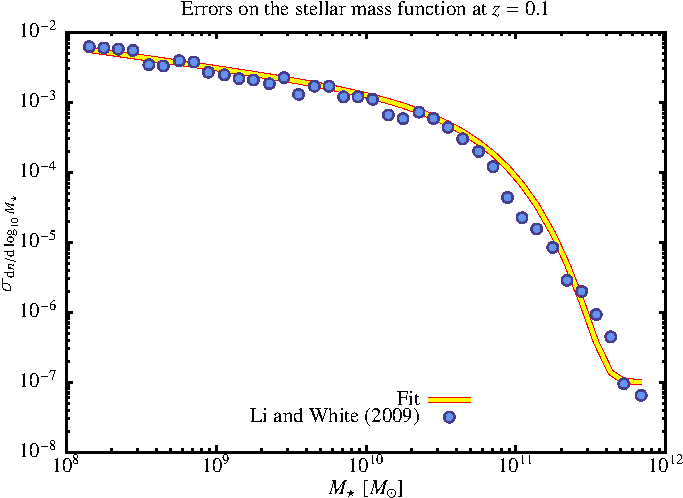
\includegraphics[width=160mm]{../plots/stellarMassFunctionErrors_z01.pdf}
 \end{center}
 \caption{Errors on the \protect\cite{li_distribution_2009} stellar mass funtion (points) and the fitting function (line) given by eqn.~(\protect\ref{eq:stellarMassFunctionErrorsFit}).}
 \label{fig:stellarMassFunctionErrors}
\end{figure}

\begin{figure}
 \begin{center}
 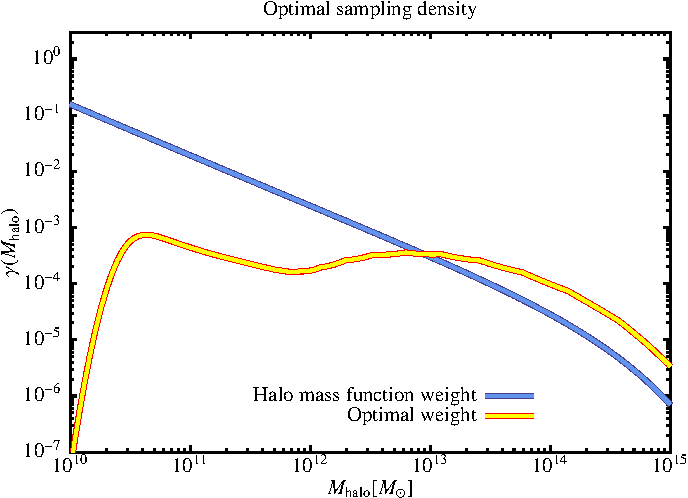
\includegraphics[width=160mm]{../plots/optimalSamplingStellarMassFunction.pdf}
 \end{center}
 \caption{Optimal weighting (yellow line) compared with weighting by the dark matter halo mass function (i.e. sampling halos at random from a representative volume; blue line). Sampling densities have been normalized to unit compute time.}
 \label{fig:optimalSamplingStellarMassFunction}
\end{figure}

\subsection{Refining by Other Merger Tree Statistics}

Since building merger trees is relatively fast, while solving the baryonic physics is slow it may be advantageous to  non-uniformly sample the distribution of merger trees at fixed merger tree mass, $M$. For example, we could assign some measure of formation history to each merger tree, such as the time since the last major merger, $\tau$. The halo mass function then becomes $n(M,\tau)$ (which can be computed by simulating large numbers of trees), and the tree sampling function becomes $\gamma(M,\tau)$. We'd then need to know the stellar mass function conditioned on both $M$ and $\tau$, $\phi_\star(M_\star|M,\tau)$. Given these, the above approach could be easily generalized to determine an optimal $\gamma(M,\tau)$. Then, after generating a merger tree, we'd first compute $\tau$. If a sufficient number of trees in that $\tau$ interval had already been computed, then we'd simply drop that tree and compute another one. The speed up here would depend on how fast building trees is relative to solving baryonic physics and what fraction of trees you discard. In principle, the trees could be generated, sampled and stored in advance so that we'd already have an optimally distributed set of trees in $M$ and $\tau$ that could be used for each model run.

\section{Constraints}\label{sec:ConstraintScripts}

Any constraint which can be applied to \glc\ is defined by two files, a configuration file and a likelihood script, which must be placed in {\tt constraints/constraints} and {\tt constraints/scripts} respectively. 

\subsection{Configuration File}\label{sec:ConstraintConfigFiles}

The configuration file should have the form:
\begin{verbatim}
<!-- Defines a constraint to match some data. -->                                          
<constraint>                                                                                                         
  <name>Long-form name of this constraint</name>                                                                      
  <label>shortLabelForThisConstraint</label>                                                                        
  <outputRedshift>0.07</outputRedshift>                                                                              
  <outputRedshift>1.00</outputRedshift>                                                                              
  <haloMassResolution>5.0e9</haloMassResolution>                                                                     
  <haloMassMinimum>2.0e10</haloMassMinimum>                                                                          
  <haloMassMaximum>2.0e14</haloMassMaximum>                                                                          
  <analysis>constraints/scripts/myAnalysisScript.pl</analysis>                                         
  <luminosity>
    <filter>UKIRT_K</filter>
    <redshift>0.0</redshift>
    <frame>rest</frame>
  </luminosity>
  <luminosity>
    <filter>UKIRT_K</filter>
    <redshift>1.0</redshift>
    <frame>observed</frame>
  </luminosity>
  <optionOn>outputMainBranchStatus</optionOn>
  <optionOn>outputDensityContrastData</optionOn>
  <parameter>
   <name>outputDensityContrastValues</name>
   <value>200.0</value>
   <accumulation>unique</accumulation>
  </parameter>
</constraint>                                                                                                        
\end{verbatim}
The {\tt name} and {\tt label} are used to describe the constraint ({\tt label} is used as a suffix in file names so should not contain spaces or other characters which might cause problems in file names). 

The remaining elements describe the requirements for this constraint. {\tt haloMassResolution} specifies the maximum resolution in mergers trees that still allows this constraint to be computed accurately. Similarly, {\tt haloMassMinimum} and {\tt haloMassMaximum} specify the required range of halo masses to simulate to allow this constraint to be computed accurately.

One or more {\tt outputRedshift} elements may be present, each specifying a redshift at which output is required for this constraint. Similarly, one or more {\tt luminosity} elements may be present, each of which specifies a luminosity which must be computed for this constraint. Each {\tt luminosity} must contain a specification of {\tt filter}, {\tt redshift}, and {\tt frame} to define which luminosity is to be computed.

One or more {\tt optionOn} elements may be present. Each element must specify the name of a \glc\ input parameter. That parameter will be set to {\tt true} in the \glc\ input parameter file.

Finally, arbitrary other parameter may be set using the standard {\tt parameter} element which should give the {\tt name} and {\tt value} for the parameter. Optionally, an {\tt accumulation} element may also be specified for each {\tt parameter}. This controls how values of the parameter are to be accumulated if set by more than one constraint. An accumulation of {\tt overwrite} will simply overwrite any previously set values. An accumulation of {\tt combine} will concatenate all values set by different constraints. Finally, an accumulation of {\tt unique} will concatenate all values set by different constraints and then filter out any duplicates.

When multiple constraints are used, their requirements are automatically combined.

\subsection{Likelihood Script}

The likelihood script for a constraint is required to perform several tasks, controlled by command line options. The script should accept the following command line syntax:
\begin{verbatim}
 myScript.pl <galacticusFile> [options...]
\end{verbatim}
where {\tt galacticusFile} is the file name of the \glc\ model for which the likelihood calculation should be performed. The following options must be supported by the script:
\begin{description}
 \item [{\tt --plotFile <fileName>}] If this option is present, the script should generate a plot showing the constraint and the model result and write it to {\tt fileName}.
 \item [{\tt --outputFile <fileName>}] If this option is present, the script should compute the log-likelihood of the model given the constraint and write it to {\tt fileName} using the format
\begin{verbatim}
 <constraint>
  <logLikelihood>-123</logLikelihood>
 </constraint>
\end{verbatim}
 \item [{\tt --accuracyFile <fileName>}] If this option is present, the script should write an XML file giving details of the accuracy of the model results relative to the observational errors using the format
\begin{verbatim}
 <accuracy>
  <x>...</x>
  .
  .
  .
  <x>...</x>
  <yModel>...</yModel>
  .
  .
  .
  <yModel>...</yModel>
  <yData>...</yData>
  .
  .
  .
  <yData>...</yData>
  <errorModel>...</errorModel>
  .
  .
  .
  <errorModel>...</errorModel>
  <errorData>...</errorData>
  .
  .
  .
  <errorData>...</errorData>
 </accuracy>
\end{verbatim}
In this file the {\tt yModel} and {\tt yData} elements should give the values of the model result and the comparable data respectively, while {\tt errorModel} and {\tt errorData} should give an estimate of the errors on these quantities. In the case of the model error this should include only the contribution arising from the finite number of merger trees simulated. This file will be used to judge whether the model is running sufficient merger trees such that the likelihood is not dominated by these errors. The {\tt x} elements are optional but can be used to give the parameter values associated with each model result.
 \item [{\tt --resultFile <fileName>}] If this option is present, the script should write an XML file giving details of the result of the model using the format
\begin{verbatim}
 <accuracy>
  <x>...</x>
  .
  .
  .
  <x>...</x>
  <y>...</y>
  .
  .
  .
  <y>...</y>
  <error>...</error>
  .
  .
  .
  <error>...</error>
 </accuracy>
\end{verbatim}
In this file the {\tt y} elements should give the values of the model result, while the {\tt error} elements should give an estimate of the errors on these results. The error should include only the contribution arising from the finite number of merger trees simulated. This file will be used to judge whether the model result is converged with respect to various numerical parameters in \glc. The {\tt x} elements are optional but can be used to give the parameter values associated with each model result.
 \item [{\tt --modelDiscrepancies <path>}] If this option is present, the script should scan {\tt path}. For each directory found in {\tt path} the script should check for the existance of a file named {\tt discrepancy<label>.hdf5} where {\tt label} is the label given for this constraint in its configuration file (see \S\ref{sec:ConstraintConfigFiles}). If present, the model discrepancy given in that file should be applied to the likelihood calculation. See \S\ref{sec:ModelDiscrepancy} for a description of the structure of the discrepancy files.
\end{description}

\subsection{Available Constraints}

\subsubsection{Li \& White (2009) SDSS Stellar Mass Function}

This constraint utilizes the stellar mass function for $z\approx 0.07$ galaxies measured by \cite{li_distribution_2009} from the \gls{sdss}. The mass function reported by \cite{li_distribution_2009} is converted to the appropriate Hubble constant for the given \glc\ model (assuming that masses scale as $H_0^{-2}$ and volumes as $H_0^3$)---no adjustment is made for cosmological parameters given the low redshift of the sample.

Given a \glc\ model, total stellar masses of model galaxies are adjusted using:
\begin{equation}
 M_\star \rightarrow {\bf G} {\bf S} M_\star 
\end{equation}
where the ${\bf S}$ operator is a multiplicative factor accounting for systematic errors in stellar mass determination and is equal to \citep{behroozi_comprehensive_2010}
\begin{equation}
 \log_{\rm 10} S = \mu + \kappa \log_{\rm 10} \left({M_\star \over 10^{11.3}M_\odot}\right)
\end{equation}
where $\mu=${\tt [sdssStellarMassFunctionZ0.07StellarMassSystematicMu]}, $\kappa=${\tt [sdssStellarMassFunctionZ0.07StellarMassSystematiKappa]}, and the {\bf G} operator is a multiplicative factor drawn from a log-normal distribution of width $0.07$~dex for each galaxy to mimic the effects of random errors on stellar masses (motivated by the discussion of \cite{behroozi_comprehensive_2010}).

The model masses are then used to construct a mass function by binning into a histogram using the masses reported by \cite{li_distribution_2009} (modified as described above) as the centers of the bins (with bin boundaries placed at the geometric means of consecutive bin centers).

If the {\tt --modelDiscrepancies} option is given, then any multiplicative or additive discrepancies found are applied to the model mass function, and any additional covariance is added to the covariance matrix.

The covariance matrix is computed as
\begin{equation}
 {\bf C} = {\bf C}_{\rm obs} + {\bf C}_{\rm model,random} + \sum_i {\bf C}_{{\rm discrepancy}, i},
\end{equation}
where ${\bf C}_{\rm obs}$ is the covariance matrix of the observational data, ${\bf C}_{\rm model,random}$ is the covariance matrix of the model arising from random noise (due to the finite number of trees simulated---see \S\ref{sec:AnalysisALFALFAHIMassFunction} for a description of how this covariance matrix is estimated), and ${\bf C}_{{\rm discrepancy}, i}$ is the covariance due to the $i^{\rm th}$ model discrepancy.

The model likelihood is then computed using:
\begin{equation}
 \mathcal{L} = {1 \over \sqrt{(2 \pi)^n |{\bf C}|}} \exp\left[ -{1\over 2} \Delta {\bf C}^{-1} \Delta \right],
\end{equation}
where $\Delta_i = \Phi_{{\rm model}, i} - \Phi_{{\rm observed}, i}$ is the difference between the model and observed mass functions, and $n$ is the number of points in the mass function histogram.

Computing the large-scale structure contribution to the covariance function requires integration of the non-linear matter power spectrum over the Fourier transform of the survey window function. We use the method of \cite{peacock_non-linear_1996} to determine the non-linear matter power spectrum, because of its simplicity and speed. We have checked that using a more accurate non-linear matter power spectrum (e.g. \citealt{lawrence_coyote_2010}) makes negligible difference to our results.

To find a suitable \gls{hod} to describe the galaxies in the \cite{li_distribution_2009} sample we adopt the model of \cite{behroozi_comprehensive_2010}. This is an 11 parameter model which describes separately the numbers of satellite and central galaxies occupying a halo of given mass---the reader is referred to \cite{behroozi_comprehensive_2010} for a complete description of the functional form of this parametric \gls{hod}. 

To reproduce the mass function of \cite{li_distribution_2009} using this \gls{hod} we use the \gls{bie} \citep{weinberg_computational_2012} to constrain the \gls{hod} parameters. We use a likelihood
\begin{equation}
 \ln \mathcal{L} = -{1\over 2} \Delta\cdot \mathcal{C}^{-1}\cdot \Delta^{\rm T} - {N \over 2} \ln(2\pi) - {\ln |\mathcal{C}| \over 2},
\end{equation}
where $N$ is the number of bins in the mass function, $\mathcal{C}$ is the covariance matrix of the observed mass function, and $\Delta_i = \phi_i^{\rm (HOD)} - \phi_i^{\rm (observed)}$. Of course, it is precisely this covariance matrix, $\mathcal{C}$, that we are trying to compute. We therefore adopt an iterative approach as follows:
\begin{enumerate}
 \item make an initial estimate of the covariance matrix, assuming that only Poisson errors contribute (the covariance matrix is therefore diagonal, and the terms are easily computed from the measured mass function and the survey volume as a function of stellar mass);
 \item find the maximum likelihood parameters of the \gls{hod} given the observed mass function and the current estimate of the covariance matrix;
 \item using this \gls{hod} and the framework of \cite{smith_how_2012}, compute a new estimate of the covariance matrix, including all three contributions;
 \item repeat steps 2 and 3 until convergence in the covariance matrix is achieved.
\end{enumerate}
In practice we find that this procedure leads to an \gls{hod} and covariance matrix which oscillate between two states in successive iterations. The differences in the covariance matrix are relatively small however, so we choose to conservatively adopt the covariance matrix with the larger values. In future, adding additional constraints to the \gls{hod} (as described below) should help mitigate this problem.

\subsubsection{Martin et al. (2010) ALFALFA HI Mass Function}\label{sec:AnalysisALFALFAHIMassFunction}

This constraint utilizes the HI mass function for $z\approx 0.0$ galaxies measured by \cite{martin_arecibo_2010} from the ALFALFA survey. The mass function reported by \cite{martin_arecibo_2010} is converted to the appropriate Hubble constant for the given \glc\ model (assuming that masses scale as $H_0^{-2}$ and volumes as $H_0^3$)---no adjustment is made for cosmological parameters given the low redshift of the sample.

Given a \glc\ model, total gas masses of model galaxies are adjusted using:
\begin{equation}
 M_{\rm HI} \rightarrow {\bf G} {\bf S} M_{\rm gas}
\end{equation}
where the ${\bf S}$ operator is a multiplicative factor accounting for systematic errors in HI mass determination and for the unknown molecular fraction and is equal to:
\begin{equation}
 \log_{\rm 10} S = \mu + \kappa \log_{\rm 10} \left({M_\star \over 10^9M_\odot}\right)
\end{equation}
where $\mu=${\tt [alfalfaHiMassFunctionZ0.00MolecularFractionMu]}, $\kappa=${\tt [alfalfaHiMassFunctionZ0.00MolecularFractionKappa]}, and the {\bf G} operator is a multiplicative factor drawn from a log-normal distribution. The width of this log-normal is determined from the combination of observational random errors on HI mass and scatter in the H$_2$/HI mass ratio at fixed total gas mass. Observational random errors on HI mass are taken from Fig.~19 of \cite{haynes_arecibo_2011}. We fit the magnitude of the error as a function of HI mass using a functional form:
\begin{equation}
 \sigma_{\rm obs} = a + \exp\left(-{\log_{10}(M_{\rm HI}/M_\odot)-b\over c}\right),
\end{equation}
where $\sigma_{\rm obs}$ is the error on $\log_{10}(M_{\rm HI}/M_\odot)$. We find a good fit using values of $a=0.100$, $b=5.885$, and $c=0.505$ as shown in Fig.~\ref{fig:ALFALFAErrorModel}. 

\begin{figure}
 \begin{center}
 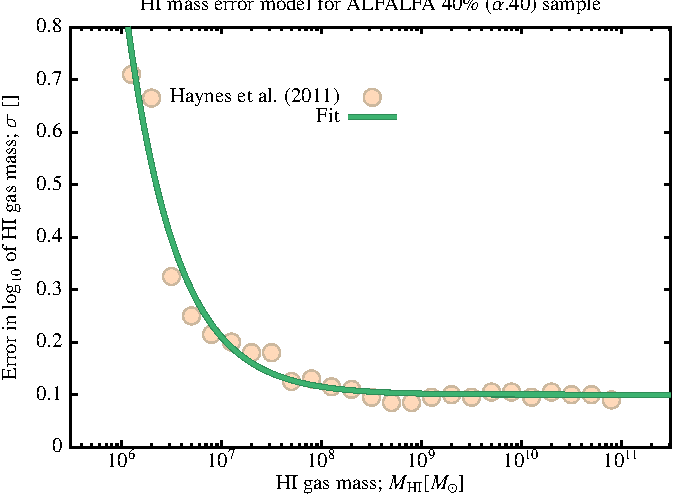
\includegraphics[width=85mm,trim=0mm 0mm 0mm 4mm,clip]{Plots/DataAnalysis/alfalfaHIMassErrorModel.pdf}
 \caption{The observational random error in galaxy HI mass as a function of HI mass for the ALFALFA survey. Points show the errors reported by \protect\cite{haynes_arecibo_2011}, while the line shows a simple functional form fit to these errors.}
 \end{center}
 \label{fig:ALFALFAErrorModel}
\end{figure}

In addition, we expect there to be significant scatter in the H$_2$/HI mass ratio at fixed total gas mass. For example, Figure~5 of \cite{power_redshift_2010} shows a broad distribution of such values. We approximate this scatter as a Gaussian random process with standard deviation $\sigma$. This random ``error'' is added in quadrature to the observational errors when constructing the mass function. For a prior on $\sigma$ we adopt a normal distribution with mean of $0.4$ (estimated from Figure~5 of \cite{power_redshift_2010}) and standard deviation $0.3$.

The model masses are then used to construct a mass function by binning into a histogram using the masses reported by \cite{martin_arecibo_2010} (modified as described above) as the centers of the bins (with bin boundaries placed at the geometric means of consecutive bin centers).

If the {\tt --modelDiscrepancies} option is given, then any multiplicative or additive discrepancies found are applied to the model mass function, and any additional covariance is added to the covariance matrix.

The covariance matrix is computed as
\begin{equation}
 {\bf C} = {\bf C}_{\rm obs} + {\bf C}_{\rm model,random} + \sum_i {\bf C}_{{\rm discrepancy}, i},
\end{equation}
where ${\bf C}_{\rm obs}$ is the covariance matrix of the observational data, ${\bf C}_{\rm model,random}$ is the covariance matrix of the model arising from random noise (due to the finite number of trees simulated, and ${\bf C}_{{\rm discrepancy}, i}$ is the covariance due to the $i^{\rm th}$ model discrepancy.

To construct ${\bf C}_{\rm model,random}$ we make use of the fact that \glc\ works by sampling a set of tree ``root masses'' from the $z=0$ dark matter halo mass function. From each root, a tree is grown, within which the physics of galaxy formation is then solved. Root masses are sampled uniformly from the halo mass function. That is, the cumulative halo mass function, $N(M)$, is constructed between the maximum and minimum halo masses to be simulated. The number of root masses, $N_{\rm r}$, to be used in a model evaluation is then determined. Root masses are then chosen such that
\begin{equation}
 N(M_i) = N(M_{\rm min}) {i-1 \over N_{\rm r}-1}
\end{equation}
for $i=1\ldots N_{\rm r}$ (noting that $N(M_{\rm max})=0$ by construction). 

Consider first those galaxies which form in the main branch of each tree (i.e. those galaxies which are destined to become the central galaxy of the $z=0$ halo). Suppose that we simulate $N_k$ halos of root mass $M_k$ at $z=0$. In such halos the main branch galaxies will, at any time, have stellar masses drawn from some distribution $p_k(M_\star|t)$. The number of such galaxies contributing to bin $i$ of the mass function is therefore binomially distributed with success probability $p_{ik} = \int_{M_{i,\rm min}}^{M_{i,\rm max}} p_k(M_\star|t) \d M_\star$ and a sample size of $N_k$. The contribution to the covariance matrix from these main branch galaxies is therefore:
\begin{equation}
 \mathcal{C}_{ij} = \left\{ \begin{array}{ll} p_{ik}(1-p_{ik}) N_k w_k^2 & \hbox{ if } i = j \\ -p_{ik} p_{jk} N_k w_k^2 & \hbox{ otherwise,} \end{array} \right.
\end{equation}
where $w_k$ is the weight to be assigned to each tree. To compute this covariance requires knowledge of the probabilities, $p_{ik}$. We estimate these directly from the model. To do this, we bin trees into narrow bins of root mass and assume that $p_{ik}$ does not vary significantly across the mass range of each bin. Using all realizations of trees that fall within a given bin, $k$, we can directly estimate $p_{ik}$.

In addition to the main branch galaxies, each tree will contain a number of other galaxies (these will be ``satellite'' galaxies at $z=0$, but at higher redshifts may still be central galaxies in their own halos). Tests have established that the number of satellites in halos is well described by a Poisson process. Note that each galaxy contributes Gaussian distribution to the mass function due to modelling of random errors in stellar mass determinations. For main branch galaxies this is simply accounted for when accumulating the probabilities, $p_{ik}$. For satellite galaxies, off-diagonal contributions to the covariance matrix arise as a result, $C_{ij} = w_k f_i f_j$, where $f_i$ is the fraction of the galaxy contributing to bin $i$ of the mass function.

The model likelihood is then computed using:
\begin{equation}
 \mathcal{L} = {1 \over \sqrt{(2 \pi)^n |{\bf C}|}} \exp\left[ -{1\over 2} \Delta {\bf C}^{-1} \Delta \right],
\end{equation}
where $\Delta_i = \Phi_{{\rm model}, i} - \Phi_{{\rm observed}, i}$ is the difference between the model and observed mass functions, and $n$ is the number of points in the mass function histogram.

Computing the large-scale structure contribution to the covariance function requires integration of the non-linear matter power spectrum over the Fourier transform of the survey window function. We use the method of \cite{peacock_non-linear_1996} to determine the non-linear matter power spectrum, because of its simplicity and speed. We have checked that using a more accurate non-linear matter power spectrum (e.g. \citealt{lawrence_coyote_2010}) makes negligible difference to our results.

To find a suitable \gls{hod} to describe the galaxies in the \cite{martin_arecibo_2010} sample we adopt the model of \cite{behroozi_comprehensive_2010}. This is an 11 parameter model which describes separately the numbers of satellite and central galaxies occupying a halo of given mass---the reader is referred to \cite{behroozi_comprehensive_2010} for a complete description of the functional form of this parametric \gls{hod}. 

To reproduce the mass function of \cite{martin_arecibo_2010} using this \gls{hod} we use the \gls{bie} \citep{weinberg_computational_2012} to constrain the \gls{hod} parameters. We use a likelihood
\begin{equation}
 \ln \mathcal{L} = -{1\over 2} \Delta\cdot \mathcal{C}^{-1}\cdot \Delta^{\rm T} - {N \over 2} \ln(2\pi) - {\ln |\mathcal{C}| \over 2},
\end{equation}
where $N$ is the number of bins in the mass function, $\mathcal{C}$ is the covariance matrix of the observed mass function, and $\Delta_i = \phi_i^{\rm (HOD)} - \phi_i^{\rm (observed)}$. Of course, it is precisely this covariance matrix, $\mathcal{C}$, that we are trying to compute. We therefore adopt an iterative approach as follows:
\begin{enumerate}
 \item make an initial estimate of the covariance matrix, assuming that only Poisson errors contribute (the covariance matrix is therefore diagonal, and the terms are easily computed from the measured mass function and the survey volume as a function of stellar mass);
 \item find the maximum likelihood parameters of the \gls{hod} given the observed mass function and the current estimate of the covariance matrix;
 \item using this \gls{hod} and the framework of \cite{smith_how_2012}, compute a new estimate of the covariance matrix, including all three contributions;
 \item repeat steps 2 and 3 until convergence in the covariance matrix is achieved.
\end{enumerate}
In practice we find that this procedure leads to an \gls{hod} and covariance matrix which oscillate between two states in successive iterations. The differences in the covariance matrix are relatively small however, so we choose to conservatively adopt the covariance matrix with the larger values. In future, adding additional constraints to the \gls{hod} (as described below) should help mitigate this problem.

\subsubsection{Shen et al. (2003) Late-Type Galaxy Size Distribution}\label{sec:SDSSLateTypeGalaxySizeDistribution}

This constraint utilizes the distribution of Petrosian half-light radii for $z\approx 0.07$ late-type galaxies measured by \cite{shen_size_2003} from the \gls{sdss}. The size function reported by \cite{shen_size_2003} is converted to the appropriate cosmology for the given \glc\ model (assuming that sizes scale as the angular diameter distance, and masses as the square of the luminosity distance).

Given a \glc\ model, total stellar masses of model galaxies are adjusted using:
\begin{equation}
 M_\star \rightarrow {\bf G} {\bf S} M_\star 
\end{equation}
where the ${\bf S}$ operator is a multiplicative factor accounting for systematic errors in stellar mass determination and is equal to \citep{behroozi_comprehensive_2010}
\begin{equation}
 \log_{\rm 10} S = \mu + \kappa \log_{\rm 10} \left({M_\star \over 10^{11.0}M_\odot}\right)
\end{equation}
where $\mu=${\tt [diskGalaxySizesSDSSZ0.07MassSystematic0]}, $\kappa=${\tt [diskGalaxySizesSDSSZ0.07MassSystematic1]}, and the {\bf G} operator is a multiplicative factor drawn from a log-normal distribution of width $0.0806$~dex for each galaxy to mimic the effects of random errors on stellar masses (motivated by the statement from \cite{shen_size_2003} who quote the 95\% confidence
interval on masses as being $\pm 40$\%).

{\bf Note:} This analysis currently assumes that model galaxies have disk Petrosian half-mass radii of
\begin{equation}
 R_{\rm 50} = 1.6676 {1 \over \sqrt{2}} \lambda R_{\rm vir}.
\end{equation}

Disk sizes of model galaxies are then adjusted using:
\begin{equation}
 R_{50} \rightarrow {\bf G} {\bf S} R_{50} 
\end{equation}
where the ${\bf S}$ operator is a multiplicative factor accounting for systematic errors in radius determination and in determination of radius from halo virial radius and spin and is equal to
\begin{equation}
 \log_{\rm 10} S = \mu + \kappa \log_{\rm 10} \left({R_{50} \over 1 \hbox{kpc}}\right)
\end{equation}
where $\mu=${\tt [iskGalaxySizesSDSSZ0.07RadiusSystematic0]}, $\kappa=${\tt [iskGalaxySizesSDSSZ0.07RadiusSystematic1]}, and the {\bf G} operator is a multiplicative factor drawn from a log-normal distribution of width $0.0128$~dex for each galaxy to mimic the effects of random errors on disk radii (estimated from the fractional errors reported in the \gls{sdss} database).

The model sizes and masses are then used to construct a mass-dependent radius function by binning into a 2-D histogram using the size and mass bins reported by \cite{shen_size_2003} (modified as described above) as the centers of the bins (with bin boundaries placed at the geometric means of consecutive bin centers).

If the {\tt --modelDiscrepancies} option is given, then any multiplicative or additive discrepancies found are applied to the model mass function, and any additional covariance is added to the covariance matrix.

The covariance matrix is computed as
\begin{equation}
 {\bf C} = {\bf C}_{\rm obs} + {\bf C}_{\rm model,random} + \sum_i {\bf C}_{{\rm discrepancy}, i},
\end{equation}
where ${\bf C}_{\rm obs}$ is the covariance matrix of the observational data, ${\bf C}_{\rm model,random}$ is the covariance matrix of the model arising from random noise (due to the finite number of trees simulated, and ${\bf C}_{{\rm discrepancy}, i}$ is the covariance due to the $i^{\rm th}$ model discrepancy.

The model covariance matrix is estimated using the sample methods as described in \S\ref{sec:AnalysisALFALFAHIMassFunction}. The only difference is that in this case we have a 2-D histogram. This 2-D histogram is ``flattened'' into a 1-D vector for purposes of likelihood computation however, so covariance matrix estimation proceeds unchanged. (Note that correlations between mass bins are accounted for, in additional to correlations between radius bins.) Since the radius functions of \cite{shen_size_2003} are normalized to unity at each mass, we must account for this in the covariance matrix. The radius function transforms as:
\begin{equation}
 f_{ik} \rightarrow {f_{ik} \over \Delta \log_{10} R \sum_i f_{ik} },
\end{equation}
where $i$ indexes radius bins, $k$ indexes mass bins, and $\Delta \log_{10} R$ is the width of the radius bin. The Jacobian of this transformation is simply
\begin{equation}
 J_{ij} = {\delta_{ij} - f_i \over  \Delta \log_{10} R \sum_i f_{ik}}.
\end{equation}
Therefore, the covariance matrix is modified according to $\mathcal{C} \rightarrow J \mathcal{C} J^{\rm T}$. The same transformation is applied to the covariance matrix of the observed data (for which the reported errors are simply the Poisson errors on each bin).

The model likelihood is then computed using:
\begin{equation}
 \mathcal{L} = {1 \over \sqrt{(2 \pi)^n |{\bf C}|}} \exp\left[ -{1\over 2} \Delta {\bf C}^{-1} \Delta \right],
\end{equation}
where $\Delta_i = \Phi_{{\rm model}, i} - \Phi_{{\rm observed}, i}$ is the difference between the model and observed mass functions, and $n$ is the number of points in the mass function histogram.

\section{Constraint Compilations}

To specify which constraints will be applied to a particular model, a compilation file is used. These must be stored in {\tt constraints/compilations}. An example of such a file follows:
\begin{verbatim}
<constraintCompilation>
  <constraint>
    <definition>constraints/constraints/stellarMassFunction_SDSS_z0.07.xml</definition>
    <weight>1.0</weight>
  </constraint>
  <constraint>
    <definition>constraints/constraints/hiMassFunction_ALFALFA_z0.00.xml</definition>
    <weight>1.0</weight>
  </constraint>
</constraintCompilation>
\end{verbatim}
Each {\tt constraint} element specifies one constraint that will be included in this compilation, and must contain a {\tt definition} element, giving the path of the configuration file for this constraint, and a {\tt weight} element which allows the relative weight given to each constraint to be varied\footnote{Note that, if your constraints are computing correct likelihoods, re-weighting them may not be a good idea. \emph{Caveat constrainor.}}.

\section{Constraint File}

\glc\ has a complete constraints infrastructure which implements various \gls{mcmc} algorithms to analyze the posterior probability distribution of the model given some compilation of constraints. The infrastructure is \gls{mpi} parallelized and ideal for running on large compute clusters.

To perform a constraint calculation simply build the constraint code:
\begin{verbatim}
 make Constrain_Galacticus.exe
\end{verbatim}
and run with a parameter file and configuration file. Typically, you will want to run this code under \gls{mpi}, for example:
\begin{verbatim}
 mpirun -n 4 Constrain_Galacticus.exe mcmcParameters.xml mcmcConfig.xml
\end{verbatim}
would run 4 processes (typically you will need to run many more than this). If running on a \gls{pbs} queue, embed this command in a suitable \gls{pbs} script and submit. 

The parameter file follows the same format as a standard \glc\ parameter file and specifies the values of parameters to be used. For example, the seed used fo pseudo-random number sequences can be specified in this file. 

The configuration file specifies the details of the constraint simulation to be performed. An example configuration file is:
\begin{verbatim}
<?xml version="1.0" encoding="UTF-8"?>
<simulationConfig>

  <likelihood>
    <type>Galacticus</type>
    <name>verySimplisticToStellarMassFunction</name>
    <compilation>stellarMassFunction_SDSS_z0.07.xml</compilation>
    <baseParameters>./mcmcWork/verySimplisticToStellarMassFunctionBase.xml</baseParameters>
    <workDirectory>./mcmcWork</workDirectory>
    <scratchDirectory>./mcmcScratch</scratchDirectory>
    <report>no</report>
    <randomize>no</randomize>
    <threads>4</threads>
    <saveState>no</saveState>
    <cpulimit>1200</cpulimit>
    <memoryLimit>2gb</memoryLimit>
    <environment>LD_LIBRARY_PATH=/opt/gcc-trunk/lib:/opt/gcc-trunk/lib64:/usr/local/upstream/lib:$LD_LIBRARY_PATH</environment>
    <environment>PATH=/opt/gcc-trunk/bin:$PATH</environment>
    <environment>GFORTRAN_ERROR_DUMPCORE=NO</environment>
  </likelihood>

  <convergence>
    <type>GelmanRubin</type>
    <Rhat>1.2</Rhat>
    <burnCount>100</burnCount>
    <testCount>100</testCount>
    <outlierCountMaximum>0</outlierCountMaximum>
    <outlierSignificance>0.95</outlierSignificance>
    <outlierLogLikelihoodOffset>60</outlierLogLikelihoodOffset>
  </convergence>
  
  <state>
    <type>history</type>
    <acceptedStateCount>100</acceptedStateCount>
  </state>
  
  <proposalSize>
    <type>adaptive</type>
    <gammaInitial>1.77</gammaInitial>
    <gammaFactor>1.414</gammaFactor>
    <acceptanceRateMinimum>0.4</acceptanceRateMinimum>
    <acceptanceRateMaximum>0.6</acceptanceRateMaximum>
    <updateCount>10</updateCount>
  </proposalSize>
  
  <randomJump>
    <type>adaptive</type>
  </randomJump>
  
  <simulation>
    <type>temperedDifferentialEvolution</type>
    <stepsMaximum>1000000</stepsMaximum>
    <stepsPostConvergence>100000</stepsPostConvergence>
    <acceptanceAverageCount>100</acceptanceAverageCount>
    <logFileRoot>./mcmcWork/mcmc/chains</logFileRoot>
    <temperatureMaximum>64.0</temperatureMaximum>
    <untemperedStepCount>20</untemperedStepCount>
    <temperedLevels>10</temperedLevels>
    <stepsPerLevel>10</stepsPerLevel>
  </simulation>

  <parameters>
    <parameter>
      <name>starFormationTimescaleDisksHaloScalingVirialVelocityExponent</name>
      <prior>
	<distribution>
	  <type>uniform</type>
	  <minimum>-6.0</minimum>
	  <maximum>+0.0</maximum>
	</distribution>
      </prior>
      <random>
	<type>Cauchy</type>
	<median>0.0</median>
	<scale>0.006</scale>
      </random>
    </parameter>
    <parameter>
      <name>starFormationTimescaleDisksHaloScalingRedshiftExponent</name>
      <prior>
	<distribution>
	  <type>uniform</type>
	  <minimum>-1.0</minimum>
	  <maximum>+4.0</maximum>
	</distribution> 
      </prior>
      <random>
	<type>Cauchy</type>
	<median>0.0</median>
	<scale>0.005</scale>
      </random>
    </parameter>
  </parameters>
  
</simulationConfig>
\end{verbatim}

The following subsections describe each entry in this file.

\subsection{{\tt likelihood}}

The {\tt likelihood} section specifies the likelihood function to be used in the simulation. The type of likelihood to use is specified by the {\tt type} element. The available choices are described in the following subsections.

\subsubsection{multivariateNormal}

The likelihood is a simple multivariate Gaussian, intended primarily for testing purposes. The distribution parameters are specified within the {\tt likelihood} element using:
\begin{verbatim}
  <mean>0.45 0.50</mean>
  <covariance>
    <row>1.0e-4 -0.9e-4</row>
    <row>-0.9e-4 1.0e-4</row>
  </covariance>
\end{verbatim}
where the {\tt mean} element gives the mean vector of $N$ elements, and the {\tt covariance} element contains $N$ {\tt row} elements each containing a vector of $N$ elements giving a single row of the covariance matrix. The likelihood is then:
\begin{equation}
\log \mathcal{L} = - {1 \over 2} \Delta \mathcal{C}^{-1} \Delta^{\rm T},
\end{equation}
where $Delta = \theta - \bar{\theta}$, $\theta$ is the state, $\bar{\theta}$ is the mean, and $\mathcal{C}$ is the covariance matrix.

\subsubsection{multivariateNormalStochastic}

The likelihood is identical to that of the {\tt multivariateNormal} class, except that the likelihood function is evaluated stochastically. In addition to the parameter of the {\tt multivariateNormal} class, two additional parameters are required and are specified within the {\tt likelihood} element using:
\begin{verbatim}
  <realizationCount>4000</realizationCount>
  <realizationCountMinimum>10</realizationCountMinimum>
\end{verbatim}
When evaluating the likelihood, the state vector is set equal to 

\begin{equation}
 S^\prime_i = \sum_{j=1}^N {2 U(S_i) \over N},
\end{equation}
where $N=${\tt realizationCount} and $U(x)$ is a uniform random deviate in the range $0$ to $x$. This results in a variance in $S^\prime_i$ of $S_i^2/3N$. This variance is added to the covariance used in evaluating the likelihood. When evaluating the likelihood at a higher temperature the number of realizations is reduced (which increases the covariance, which has the same effect as increasing the temperature) to speed computation, and the likelihood corrected for this fact. The number of realizations is reduced to $N/T$, but never allowed to fall below {\tt realizationCountMinimum}.

\subsubsection{Galacticus}

The likelihood is computed by running and analyzing a \glc\ model. The details of the model to run are specified by the follow content within the {\tt likelihood} element:
\begin{verbatim}
  <name>verySimplisticToStellarMassFunction</name>
  <compilation>stellarMassFunction_SDSS_z0.07.xml</compilation>
  <baseParameters>./mcmcWork/verySimplisticToStellarMassFunctionBase.xml</baseParameters>
  <workDirectory>./mcmcWork</workDirectory>
  <scratchDirectory>./mcmcScratch</scratchDirectory>
  <report>no</report>
  <randomize>no</randomize>
  <threads>4</threads>
  <saveState>no</saveState>
  <cpulimit>1200</cpulimit>
  <memoryLimit>2gb</memoryLimit>
  <environment>LD_LIBRARY_PATH=/opt/gcc-trunk/lib:/opt/gcc-trunk/lib64:/usr/local/upstream/lib:$LD_LIBRARY_PATH</environment>
  <environment>PATH=/opt/gcc-trunk/bin:$PATH</environment>
  <environment>GFORTRAN_ERROR_DUMPCORE=NO</environment>
\end{verbatim}

The entries have the following meanings:
\begin{description}
\item[{\tt name}] A name to use for this calculation. It will be used as the name for jobs submitted to the PBS queue for example.
\item[{\tt compilation}] Specifies the compilation file to be used for this analysis.
\item[{\tt baseParameters}] Specifies the path to a \glc\ parameter file which will be used as the base set of parameter on top of which any parameter variations will be applied.
\item[{\tt workDirectory}] The full path to a directory in which the results (e.g. \gls{mcmc} chains) will be stored.
\item[{\tt scratchDirectory}] The full path to a scratch directory where \glc\ model outputs and other temporary data will be written.
\item[{\tt report}] If set to {\tt yes}, reports additional debugging information during the run.
\item[{\tt randomize}] If {\tt yes} then each model evaluation will be performed with a different random number seed. Otherwise, the same seed is used in all cases. Experiment shows that changing the random number seed between evaluations can seriously limit the ability of \gls{mcmc} algorithms to converge.
\item[{\tt threads}] The number of parallel OpenMP threads to use for each \glc\ model. It is recommended that this be set to the number of available cores on each node, and semaphoring (see \S{sec:Semaphores}) be used. In this way, each copy of \glc\ on a node will share resources, but as one instance finishes, the others will be able to make use of the freed resources.
\item[{\tt saveState}] If {\tt yes} then \glc\ will save its internal state prior to beginning evolution of each merger tree. This is intended for debugging purposes and so should normally be set to {\tt no}.
\item[{\tt cpulimit}] A CPU time limit for each model evalulation. This can be useful if certain obscure regions of the surveyed parameter space result in unacceptably long run times. Models will be killed after this time and a very low likelihood returned.
\item[{\tt environment}] One of more such element can appear. Each specifies the value of an environment variable to be set prior to launching the \glc\ model.
\item[{\tt storeResults}] If {\tt yes} then the full results (e.g. the quantities computed to compare with observational data) from each model evalulation will be stored. Otherwise, they are discarded after each evalulation. Use {\tt yes} with caution---a typical run might include millions of model evaluations which can quickly lead to huge amounts of data being written to disk.
\end{description}

\subsection{{\tt convergence}}

The {\tt convergence} section specifies the criterion to be used to judge when the simulation has converged. The type of convergence criterion to use is specified by the {\tt type} element. The available choices are described in the following subsections.

\subsubsection{{\tt never}}

This option assumes that the simulation never converges, and so the calculation will run indefinitely. It is intended primarily for testing purposes.

\subsubsection{{\tt GelmanRubin}}

This option adopts the convergence criterion proposed by \citeauthor{gelman_a._inference_1992}~(\citeyear{gelman_a._inference_1992}; see also \citealt{brooks_general_1998}), which compares the variance in parameter values within chains to that between chains. Outlier detection is applied to the chains using a standard Grubb's outlier test. The behavior of this criterion is controlled by the following options which should be placed within the {\tt convergence} element:
\begin{description}
\item [{\tt Rhat}] The correlation coefficient, $\hat{R}$, value at which to declare convergence.
\item [{\tt burnCount}] Set number of steps to burn before applying the convergence test.
\item [{\tt testCount}] Set the number of steps between successive applications of the convergence test.
\item [{\tt outlierSignificance}] The significance level required in outlier detection.
\item [{\tt outlierLogLikelihoodOffset}] The offset in log-likelihood from the current maximum likelihood chain required for a chain to be declared to be an outlier.
\item [{\tt outlierCountMaximum}] The maximum number of outlier chains allowed.
\end{description}

\subsection{{\tt state}}

The {\tt state} section specifies the type of object used to record the state of the simulation. The type of state object to use is specified by the {\tt type} element. The available choices are described in the following subsections.

\subsubsection{{\tt simple}}

This type stores the current state but makes no attempt to record a history of the state and so cannot provide measures of the mean or variance of state over the simulation history. It does, however, maintain a running average of the state acceptance rate. The number of steps over which the acceptance rate should be computed is specified by the {\tt acceptedStateCount}.

\subsubsection{{\tt history}}

An extension of the {\tt simple} state, this type also records the mean and variance of each parameter over the history of the simulation.

\subsection{{\tt proposalSize}}

The {\tt proposalSize} section specifies the method to use when selecting the proposal size parameter, $\gamma$ (the fraction of the vector connecting to chain state to be used as the proposal for another chain), for use in differential evolution simulations. The proposal size algorithm to use is specified by the {\tt type} element. The available choices are described in the following subsections.

\subsubsection{{\tt fixed}}

This option uses a fixed $\gamma$ specified by the {\tt gamma} element.

\subsubsection{{\tt adaptive}}

This option adaptively changes $\gamma$ in an attempt to maintain the acceptance rate at an acceptable level. The algorithm is controlled by the following parameters (to be specified as elements within the {\tt proposalSize} element):
\begin{description}
\item[{\tt gammaInitial}] The initial value for $\gamma$.
\item[{\tt gammaFactor}] The multiplicative factor by which $\gamma$ should be increased or decreased if the acceptance rate is out of range.
\item[{\tt gammaMinimum}] The smallest value allowed for $\gamma$.
\item[{\tt gammaMaximum}] The largest value allowed for $\gamma$.
\item[{\tt acceptanceRateMinimum}] The minimum acceptance rate to accept before reducing $\gamma$.
\item[{\tt acceptanceRateMaximum}] The maximum acceptance rate to accept before reducing $\gamma$.
\item[{\tt updateCount}] The number of steps between successive checks of the acceptance rate.
\end{description}

\subsection{{\tt proposalSizeTemperatureExponent}}

The {\tt proposalSizeTemperatureExponent} section specifies the method to use when selecting the exponent, $\alpha$, for the temperature scaling of the proposal size parameter, $\gamma$ (the fraction of the vector connecting to chain state to be used as the proposal for another chain), for use in tempered differential evolution simulations. The proposal size temperature exponent algorithm to use is specified by the {\tt type} element. The available choices are described in the following subsections.

\subsubsection{{\tt fixed}}

This option uses a fixed $\alpha$ specified by the {\tt alpha} element.

\subsubsection{{\tt adaptive}}

This option adaptively changes $\alpha$ in an attempt to maintain the gradient of the acceptance rate with the logarithm of temperature, ${\rm d} R/{\rm d}\ln T$, at an acceptable level. The algorithm is controlled by the following parameters (to be specified as elements within the {\tt proposalSizeTemperatureExponent} element):
\begin{description}
\item[{\tt exponentInitial}] The initial value for $\alpha$;
\item[{\tt exponentFactor}] The additive factor by which $\alpha$ should be increased or decreased if the acceptance rate gradient is out of range;
\item[{\tt exponentMinimum}] The smallest value allowed for $\alpha$;
\item[{\tt exponentMaximum}] The largest value allowed for $\alpha$;
\item[{\tt acceptanceRateMinimum}] The minimum acceptance rate gradient to accept before reducing $\alpha$;
\item[{\tt acceptanceRateMaximum}] The maximum acceptance rate gradient to accept before reducing $\alpha$;
\item[{\tt updateCount}] The number of steps between successive checks of the acceptance rate gradient.
\end{description}


\subsection{{\tt randomJump}}

The {\tt randomJump} section specifies the method to use when adding a random jump component to proposals in differential evolution simulations. The random jump algorithm to use is specified by the {\tt type} element. The available choices are described in the following subsections.

\subsubsection{{\tt simple}}

The random jumps are drawn directly from the distributions specified in the {\tt random} element of each parameter (see \S\ref{sec:ParametersPriors}).

\subsubsection{{\tt adaptive}}

The random jumps are drawn from the distributions specified in the {\tt random} element of each parameter (see \S\ref{sec:ParametersPriors}) and then multiplied by the currently occupied range of each parameter (i.e. the maximum value of the parameter over all current chain states minus the minimum value of each parameter over all current chain states).

\subsection{{\tt simulation}}

The {\tt simulation} section specifies the algorithm to use to perform the simulation. The simulation algorithm to use is specified by the {\tt type} element. The available choices are described in the following subsections.

\subsubsection{{\tt differentialEvolution}}

This option uses the differential evolution algorithm of \cite{terr_braak_markov_2006}. Multiple, parallel chains are run and proposals are constructed by selecting two chains at random, taking a fraction, $\gamma$, of the vector connecting the two chain states and adding this to the state of the current chain. The details of the algorithm are controlled by the following elements which should be embedded within the {\tt simulation} element:
\begin{description}
\item[{\tt stepsMaximum}] The maximum number of steps to take.
\item[{\tt stepsPostConvergence}] The number of steps to perform after convergence is attained.
\item[{\tt acceptanceAverageCount}] The number of steps over which to average the acceptance rate.
\item[{\tt stateSwapCount}] The number of steps after which to set $\gamma=1$ to allow chains to swap states.
\item[{\tt logFileRoot}] The full path and root name of a file to log results to. The actual file name will have the rank of the \gls{mpi} process appended to it.
\end{description}

\subsubsection{{\tt temperedDifferentialEvolution}}

This option extends the {\tt differentialEvolution} option to include tempering during which the likelihood function is heated up and cooled down to allow chains to more easily walk through the likelihood landscape. In addition to the options for the {\tt differentialEvolution} algorithm, the details of the algorithm are controlled by the following elements whichy should be embedded within the {\tt simulation} element:
\begin{description}
\item[{\tt untemperedStepCount}] The number of untempered (i.e. $T=1$) steps to take between tempering cycles.
\item[{\tt temperatureMaximum}] The maximum temperature to use when tempering.
\item[{\tt temperedLevels}] The number of tempered levels to use.
\item[{\tt stepsPerLevel}] The number of differential evolution steps to take at each tempering level.
\end{description}

In each tempering cycle, the temperature is raised through levels $1$\ldots$N$ (where $N=${\tt temperedLevels}), and then back down through levels $N-1$\ldots$1$. The temperature at level $i$ is given by:
\begin{equation}
\log T_i = {i \over N} \log T_{\rm max},
\end{equation}
where $T_{\rm max}=${\tt temperatureMaximum}. During tempered steps, the $\gamma$ parameter of the differential evolution algorithm is increased by a factor $T^\alpha$, where $\alpha$ is provided by the {\tt proposalSizeTemperatureExponent} class. A value of $\alpha=1/2$ is optimal for a Gaussian likelihood.

\subsection{Parameters and Priors}\label{sec:ParametersPriors}

The {\tt parameters} section contains a list of all parameters to be varied in the analysis. Each parameter is described by one {\tt parameter} element. That element must contain a {\tt name} element, which gives the name of the parameter, a {\tt prior} element that contains a {\tt distribution} element defining the distribution for this prior, and (for differential evolution simulations) a {\tt random} element that defines the distribution to be used for the random perturbation to be added to this parameter in proposals.

\subsubsection{Loading External Parameters/Priors}

It is also possible to load parameters and their priors from external files. This is useful to add common sets of parameters, such as cosmological parameter. To do so, add an element of the form:
\begin{verbatim}
<xi:include href="../../constraints/parameters/wmap9Cosmology.xml" 
   xmlns:xi="http://www.w3.org/2001/XInclude" />
\end{verbatim}
\emph{after} the {\tt parameters} section of the constraint file. The {\tt href} attribute must give the path (relative to the constraint file, or absolute) to the external parameter file. This file should contain its own {\tt parameters} block, describing all parameters to be varied along with their priors. 

\subsubsection{Derived Parameter Values}

It is possible to define parameters in terms of other parameters. Common uses for this include:
\begin{itemize}
 \item Setting $\Omega_\Lambda$ from the value of $\Omega_{\rm M}$ to enforce a flat Universe;
 \item Setting the values of parameters with correlated priors as linear combinations of dummy parameters for which the priors are independent.
\end{itemize}
To define a parameter in this way include a {\tt parameter} element of the form:
\begin{verbatim}
<parameter>
 <name>sigma_8</name>
 <define>0.8178+%cosmology0*0.003817+%cosmology1*0.007931+%cosmology2*0.01002
    +%cosmology3*0.001584+%cosmology4*0.002931+%cosmology5*0.001727</define>
</parameter>
\end{verbatim}
Here the {\tt define} element gives an equation for the parameter in terms of other parameters. All standard mathematical operators and functions (as recognized by Perl) can be used, and other parameters referenced by using their name prefixed with a ``\%''.

\subsubsection{Including External Parameters}

Predefined sets of parameters (along with their priors) can be included using the {\tt xi:include} element. For example,
\begin{verbatim}
 <xi:include href="../../constraints/parameters/wmap7Cosmology.xml"
    xmlns:xi="http://www.w3.org/2001/XInclude" />
\end{verbatim}
will include a set of parameters from the file {\tt ../../constraints/parameters/wmap7Cosmology.xml} which defines priors on cosmological parameters consistent with the covariance matrix of the WMAP-7 cosmological constraints \citep{komatsu_seven-year_2010}.

\subsection{Distributions}

Various distribution functions (for priors and random perturbations) are supported. Where needed, the type of distribution should be specified in a {\tt type} element. Additional parameters of the distribution are specified using the elements described in the following subsections.

\subsubsection{{\tt uniform}}

A uniform distribution over a finite range
\begin{equation}
P(x) \propto \left\{ \begin{array}{ll} 1 & \hbox{ if } x_{\rm l} \leq x \leq x_{\rm u} \\ 0 & \hbox{ otherwise.}  \end{array} \right.
\end{equation}
Specified using:
\begin{description}
\item[{\tt minimum}] The lower limit of the range, $x_{\rm l}$;
\item[{\tt maximum}] The upper limit of the range, $x_{\rm u}$.
\end{description}

\subsubsection{{\tt logUniform}}

A distribution uniform in the logarithm of $x$ over a finite range
\begin{equation}
P(x) \propto \left\{ \begin{array}{ll} x^{-1} & \hbox{ if } x_{\rm l} \leq x \leq x_{\rm u} \\ 0 & \hbox{ otherwise.}  \end{array} \right.
\end{equation}
Specified using:
\begin{description}
\item[{\tt minimum}] The lower limit of the range, $x_{\rm l}$;
\item[{\tt maximum}] The upper limit of the range, $x_{\rm u}$.
\end{description}

\subsubsection{{\tt normal}}

A normal distribution, optionally with lower and upper limits:
\begin{equation}
P(x) \propto \left\{ \begin{array}{ll} \exp[-(x-\mu)^2/2S] & \hbox{ if } x_{\rm l} \leq x \leq x_{\rm u} \\ 0 & \hbox{ otherwise.}  \end{array} \right.
\end{equation}
Specified using:
\begin{description}
\item[{\tt mean}] The mean, $\mu$;
\item[{\tt variance}] The variance, $S$;
\item[{\tt minimum}] The lower limit of the range, $x_{\rm l}$;
\item[{\tt maximum}] The upper limit of the range, $x_{\rm u}$.
\end{description}

\subsubsection{{\tt Cauchy}}

A Cauchy distribution:
\begin{equation}
P(x) \propto \left[1+{x-x_0\over\gamma}\right]^{-1}.
\end{equation}
Specified using:
\begin{description}
\item[{\tt median}] The median, $x_0$;
\item[{\tt scale}] The scale, $\gamma$;
\end{description}

\subsubsection{{\tt StudentT}}

Student's t-distribution:
\begin{equation}
P(x) \propto \left(1 + {x^2\over \nu}\right)^{-(\nu+1)/2}
\end{equation}
Specified using:
\begin{description}
\item[{\tt degreesOfFreedom}] The number of degrees of freedom, $\nu$.
\end{description}


\part{Physical Implementation}

In this Part we describe the physical implementation of galaxy formation in \glc, including all components and their properties and additional output quantities from the code.

\chapter{Definitions and Conventions Used in \glc}

\glc\ adopts various definitions and conventions internally. These are explained below.

\section{Halo Masses and Dark Matter Mass}

Halo masses require some care in specifying exactly what mass they represent due to the way in which merger trees are typically created. For example, when merger trees are extracted from N-body simulations, those simulations frequently represent \emph{all} matter as collisionless. That is, the simulation contains a density $\Omega_\mathrm{M}=\Omega_\mathrm{DM}+\Omega_\mathrm{b}$ which is the sum of dark and baryonic matter densities, but all of this mass is represented as collisionless particles. Similarly, masses in merger trees built through Monte Carlo techniques typically represent all mass as collisionless.

The exact way in which masses within \glc\ are defined and used in specified in the following subsections.

\subsection{Masses in the Basic Component}

The {\normalfont \ttfamily basic} component (see \S\ref{sec:ComponentBasicProperties}) tracks the mass of each halo as defined in the merger tree. As such, it should be considered to be the mass which the halo would have if baryonic matter behaved just as dark matter. Note that these masses are inclusive of subhalos---that is, the mass of a host halo includes the mass of all of its subhalos.

\subsection{Dark Matter Profiles}

The dark matter profile functions (see \refPhysics{darkMatterProfileDMO}) return masses and densities etc. which are normalized to match the mass of the {\normalfont \ttfamily basic} component at the virial radius of the halo. As such, their returned values should be considered to represent the case where baryonic matter behaves as dark matter. This is a convention, and is useful for calculations of large scale structure for example.

\subsection{Galactic Structure Functions}

The various galactic structure functions assume that the masses/densities/etc. reported by the dark matter profile functions should be scaled by a factor $(\Omega_\mathrm{M}-\Omega_\mathrm{b})/\Omega_\mathrm{b}$ to leave only the dark matter part of the profile. Baryonic contributions to the mass/density/etc. will be provided by the components representing those mass distributions.

\subsection{Satellite Virial Orbits}

These functions (see \refPhysics{virialOrbit}) typically use the {\normalfont \ttfamily basic} component mass in determining parameters of an orbit, since they are typically calibrated to simulations of collisionless matter only.

\subsection{Satellite Merging Timescales}

These functions (see \refPhysics{satelliteMergingTimescales}) typically use the {\normalfont \ttfamily basic} component mass in determining parameters of an orbit, since they are typically calibrated to simulations of collisionless matter only.

\subsection{Dynamical Friction}

These functions (see \refPhysics{satelliteDynamicalFriction}) evaluate densities through the relevant galactic structure function, and so correctly account for the fraction of the {\normalfont \ttfamily basic} component mass which is in the form of dark matter.

\subsection{Galactic Structure Radius Solvers}

These functions \refPhysics{galacticStructureSolver}) determine the radii of galactic components (such as disk and spheroid), typically by iteratively seeking a solution in which their angular momenta and radii are consistent (assuming rotational support) with the net gravitational potential of the entire system (galaxy plus dark matter halo).

\section{Luminosity Units}

Galaxy luminosities are output in the \gls{ABmagnitude} system, such that a luminosity of $1$ corresponds to an object of $0^\mathrm{th}$ absolute magnitude in the \gls{ABmagnitude} system. This implies that the luminosities are in units of $4.4659\times 10^{13}$~W/Hz.

\section{Peculiar Velocities}\label{sec:GalacticusVelocityDefinitions}\hyperdef{sec}{peculiarVelocities}{}

Velocities in \glc\ are always \emph{physical} velocities. When reading merger tree properties (including velocities) from file it is often convenient to store velocities without the Hubble flow contribution, as ``peculiar velocities'', in the file---see \href{https://github.com/galacticusorg/galacticus/wiki/Merger-Tree-File-Format#forest-halos-group}{here} for how to specify whether or not  the velocities included in the file include the Hubble flow or not.

If peculiar velocities are stored it is important to use the same definition of peculiar velocity as is used by \glc. Defining $t$ to be physical time and $\mathbf{x}$ to be comoving position, \glc\ uses the conventional definition of peculiar velocity in a cosmological context, namely that it is the deviation of the physical velocity from the Hubble flow. Physical coordinates are given by $\mathbf{r} = a\mathbf{x}$, so the peculiar velocity is
\begin{equation}
\mathbf{v}_\mathrm{pec} \equiv {\mathrm{d} \mathbf{r} \over \mathrm{d} t} - H \mathbf{r} = a {\mathrm{d} \mathbf{x}\over\mathrm{d} t} = {\mathrm{d}\mathbf{x}\over\mathrm{d}\eta},
\end{equation}
where $\mathrm{d}\eta = \mathrm{d}t/a$ is conformal time. 

\section{Gravitational Potentials}\index{potential!gravitational}\index{gravitational potential}

Gravitational potentials are measured in velocity units (i.e. km$^2$/s$^2$), and the arbitrary constant offset is chosen such that the total gravitational potential in any halo at the virial radius is $\Phi(r_\mathrm{virial})=-V_\mathrm{virial}^2$. This choice is made for two reasons:
\begin{enumerate}
\item some mass distributions used have potentials which diverge as $r\rightarrow\infty$, so the usual choice of $\Phi(r) \rightarrow 0$ as $r \rightarrow \infty$ is not applicable;
\item this choice is consistent with the potential at the virial radius of the halo considered as a point mass as is used in Keplerian orbit calculations.
\end{enumerate}
Note that the choice of constant offset for the potential of any mass distribution or galactic component is irrelevant---the galactic structure function which computes potential will ensure that the potential is always offset to match the definition given above.

\section{Radius Specifiers}\label{sec:radiusSpecifiers}\index{radii!specifiers}\hyperdef{sec}{radiusSpecifiers}{}

Several \refClass{nodePropertyExtractorClass}s extract properties at one or more radii in a node. \glc\ provides a flexible way of specifying such radii as fractions of physical quantities such as the virial radius, disk half-mass radius, etc.

Each radius specifier should take the form:
\begin{verbatim}
  radiusType:componentType:massType:radius
\end{verbatim}
The elements of this colon-separated specifier determine the radius at which a property is computed, which components/mass types should be counted, and whether baryonic loading of the halo should be accounted for. The elements have the following meaning:
\begin{description}
 \item [{\normalfont \ttfamily radius}] the numerical value of the radius at which to compute the property (with units specified by the {\normalfont \ttfamily radiusType} element);
 \item [{\normalfont \ttfamily radiusType}] specifies the units of the {\normalfont \ttfamily radius} element---valid options are {\normalfont \ttfamily diskRadius}, {\normalfont \ttfamily hotHaloOuterRadius}, {\normalfont \ttfamily diskHalfMassRadius}, {\normalfont \ttfamily spheroidRadius}, {\normalfont \ttfamily spheroidHalfMassRadius}, {\normalfont \ttfamily darkMatterScaleRadius}, {\normalfont \ttfamily virialRadius}, just {\normalfont \ttfamily radius} (which implies radii are given in units of Mpc), {\normalfont \ttfamily galacticMassFraction\{\textless fraction\textgreater\}}, {\normalfont \ttfamily stellarMassFraction\{\textless fraction\textgreater\}}, or \newline {\normalfont \ttfamily galacticLightFraction\{\textless fraction\textgreater\}\{\textless luminosity\textgreater\}}, where the final three form specify a radius containing a fixed {\normalfont \ttfamily \textless fraction\textgreater} of the galactic or stellar mass, or light respectively (for the case of galactic light, {\normalfont \ttfamily \textless luminosity\textgreater} specifies the band, e.g. {\normalfont \ttfamily SDSS\_r:rest:z0.0000});
 \item [{\normalfont \ttfamily componentType}] specifies which components of the node should be counted---allowed values are {\normalfont \ttfamily all}, {\normalfont \ttfamily disk}, {\normalfont \ttfamily spheroid}, {\normalfont \ttfamily hotHalo}, {\normalfont \ttfamily darkHalo}, and {\normalfont \ttfamily blackHole};
 \item [{\normalfont \ttfamily massType}] specifies which types of mass should be counted---allowed values are {\normalfont \ttfamily all}, {\normalfont \ttfamily dark}, {\normalfont \ttfamily baryonic}, {\normalfont \ttfamily galactic}, {\normalfont \ttfamily gaseous}, {\normalfont \ttfamily stellar}, and {\normalfont \ttfamily blackHole}.
\end{description}

\section{Half-mode and quarter-mode masses}
For non-cold dark matter models with a matter power spectrum suppressed on small scales, a characteristic suppression scale can be defined by comparing the linear transfer function with that in the\gls{cdm} model. A popular definition is the half-mode (quarter-mode) mass, which corresponds to the wavenumber at which the transfer function is suppressed by a factor of two (four) relative to a \gls{cdm} transfer function.



\chapter{Node Components}\label{sec:Components}

In addition to the implementations described here, each component class has a ``{\normalfont \ttfamily null}'' implementation. Selecting this implementation---which has no properties and does not respond to any events---effectively switches off the relevant component class. Of course, this is safe only if none of the other active implementations expect to get or set properties of the component class (or if they rely on a sensible implementation of that class).

\section{(Supermassive) Black Hole}

\subsection{``Standard'' Implementation}

\subsubsection{Properties}

The standard black hole implementation defines the following properties:
\begin{description}
 \item [{\normalfont \ttfamily mass}] The mass of the black hole: $M_\bullet$ {\normalfont \ttfamily [blackHoleMass]}.
 \item [{\normalfont \ttfamily spin}] The spin of the black hole, $j_\bullet$ {\normalfont \ttfamily [blackHoleSpin]}.
 \item [{\normalfont \ttfamily radialPosition}] The radial position of the black hole: $r_\bullet$ {\normalfont \ttfamily [blackHoleRadialPosition]} 
\end{description}

\subsubsection{Initialization}

Black holes are not initialized, they are created (with a seed mass given by {\normalfont \ttfamily blackHoleSeedMass} and zero spin) as needed.

\subsubsection{Differential Evolution}

In the standard black implementation the mass and spin evolve as:
\begin{eqnarray}
\dot{M}_\bullet &=& (1-\epsilon_{\mathrm radiation}-\epsilon_{\mathrm jet}) \dot{M}_0 \\
\dot{j}_\bullet &=& \dot{j}(M_\bullet,j_\bullet,\dot{M}_0),
\end{eqnarray}
where $\dot{M}_0$ is the rest mass accretion rate, $\epsilon_{\mathrm radiation}$ is the radiative efficiency of the accretion flow feeding the black hole, $\epsilon_{\mathrm jet}$ is the efficiency with which accretion power is converted to jet power and $\dot{j}(M_\bullet,j_\bullet,\dot{M}_0)$ is the spin-up function of that accretion flow (see \S\ref{sec:AccretionDisks}). The rest mass accretion rate is computed assuming Bondi-Hoyle-Lyttleton accretion from the spheroid gas reservoir (with an assumed temperature of {\normalfont \ttfamily [bondiHoyleAccretionTemperatureSpheroid]}) enhanced by a factor of {\normalfont \ttfamily [bondiHoyleAccretionEnhancementSpheroid]} and from the host halo (with whatever temperature that hot halo temperature profile specifies; see \S\ref{sec:HotHaloTemperature}) enhanced by a factor of {\normalfont \ttfamily [bondiHoyleAccretionEnhancementHotHalo]}. For accretion from the hot halo, the Bondi radius is limited to the outer radius of the hot halo. Additionally, the accretion rate is limited to:
\begin{equation}
 \dot{M}_{\mathrm 0,~hot~halo,~maximum} = M_{\mathrm hot}/\tau_{\mathrm sound~crossing},
\end{equation}
where $\tau_{\mathrm sound~crossing}=r_{\mathrm hot~halo~outer}/c_{\mathrm s}$ where $r_{\mathrm hot~halo~outer}$ is the outer radius of the hot halo and $c_{\mathrm s}$ is the speed of sound in the hot halo.

If {\normalfont \ttfamily [bondiHoyleAccretionHotModeOnly]}$=${\normalfont \ttfamily true} then the accretion occurs only from that fraction of the hot halo gas which was accreted in the ``hot mode'', otherwise accretion 
occurs from the entirety of the hot halo reservoir. In the first case a simple estimate of the hot mode fraction is made:
\begin{equation}
f_{\mathrm hot} = \left\{ \begin{array}{ll} 1 & \hbox{ if } x < 0.9 \\ y(x)^2[2 y(x) - 3]+1  & \hbox{ if } 0.9 \le x \le 1.0 \\ 0 & \hbox{ if } x > 1.0, \end{array} \right.
\end{equation}
where $x = r_{\mathrm cool}/r_{\mathrm virial}$ and $y(x)=[x-0.9]/[1.0-0.9]$.

The rest mass accretion rate is removed (as a mass sink) from the spheroid and hot halo components appropriately. The black hole is assumed to cause feedback in two ways:
\begin{description}
 \item [Radio-mode] If {\normalfont \ttfamily [blackHoleHeatsHotHalo]}$=${\normalfont \ttfamily true} then any jet power from the black hole-accretion disk system (see \S\ref{sec:CircumnuclearDisks}) is included in the hot halo heating rate providing that the halo is in the slow cooling regime\footnote{Specifically, the jet power multiplied by $f_{\mathrm hot} [(M_{\mathrm hot}/M_{\mathrm total}) (\Omega_{\mathrm M}/\Omega_{\mathrm b})]^2$ is added to the hot halo heating rate. The dependence on the gas fraction in the hot halo ensures that the heating rate goes smoothly to zero as the hot halo becomes depleted of gas.}\index{feedback!AGN}\index{active galactic nuclei (AGN)!feedback} (i.e. if the cooling radius is smaller than the virial radius; see, for example, \citealt{benson_cold_2010});
 \item [Quasar-mode] A mechanical wind luminosity of \citep{ostriker_momentum_2010}
\begin{equation}
 L_{\mathrm wind} = \epsilon_{\bullet, {\mathrm wind}} H(\epsilon_{\mathrm radiation},1,s) \dot{M}_0 \clight^2,
\end{equation}
where $\epsilon_{\bullet {\mathrm wind}}=${\normalfont \ttfamily [blackHoleWindEfficiency]} is the black hole wind efficiency,\newline $s$={\normalfont \ttfamily blackHoleWindEfficiencyScalesWithRadiativeEfficiency}, and
\begin{equation}
H(a,b,c) = \left\{\begin{array}{ll}a & \hbox{ if } c=\hbox{\normalfont \ttfamily true} \\b & \hbox{ if } c=\hbox{\normalfont \ttfamily false},\end{array}\right.
\end{equation}
is added to the gas \gls{component} of the spheroid (which, presumably, will respond with an outflow for example---see \S\ref{sec:ComponentSpheroid} for details of how specific implementations of the spheroid component respond to the addition of energy) if and only if the wind pressure (at the spheroid characteristic radius) is less than the typical thermal pressure in the spheroid gas \citep{ciotti_feedbackcentral_2009}, i.e.
\begin{eqnarray}
 P_{\mathrm wind} &<& P_{\mathrm ISM} \nonumber \\
 \frac{1}{2}\rho_{\mathrm wind} V_{\mathrm wind}^2 &<& {3 {\mathrm k_B} T_{\mathrm ISM} \langle \rho_{\mathrm ISM}\rangle \over 2 m_{\mathrm H}}.
\end{eqnarray}
Since $\Omega r^2 \rho_{\mathrm wind} V_{\mathrm wind}^3 = L_{\mathrm wind}$ where $\Omega$ is the solid angle of the wind flow, this can be rearranged to give $\langle\rho_{\mathrm ISM}\rangle > \rho_{\mathrm wind, critical}$ where
\begin{equation}
\rho_{\mathrm wind,critical} = {2 m_{\mathrm H} L_{\mathrm wind} \over 3 \Omega r^2 V_{\mathrm wind} {\mathrm k_B} T_{\mathrm ISM}}.
\end{equation}
This critical wind density is computed at the characteristic radius of the spheroid, $r_{\mathrm spheroid}$, assuming $V_{\mathrm wind}=10^4$km/s, $T_{\mathrm ISM}=10^4$K and $\Omega=\pi$, and the \gls{ism} density is approximated by
\begin{equation}
 \langle\rho_{\mathrm ISM}\rangle = {3 M_{\mathrm gas, spheroid} \over 4 \pi} r_{\mathrm spheroid}^3.
\end{equation}
For numerical ease, the fraction, $f_{\mathrm wind}$, of the wind luminosity added to the spheroid is adjusted smoothly through the $\rho_{\mathrm ISM}\approx\rho_{\mathrm wind,critical}$ region according to
\begin{equation}
 f_{\mathrm wind} = \left\{ \begin{array}{ll} 0 & \hbox{ if } x < 0, \\ 3x^2-2x^3 & \hbox{ if } 0 \le x \le 1, \\ 1 & \hbox{ if } x > 1, \end{array} \right.
\end{equation}
where $x=\rho_{\mathrm ISM}/\rho_{\mathrm wind,critical}-1/2$.
\end{description}

The radial position, $r_\bullet$, evolves according to the selected radial migration method (see \S\ref{sec:SMBHRadialMotion}).

Interactions between black hole triplets are accounted for if {\normalfont \ttfamily [tripleBlackHoleInteraction]}$=${\normalfont \ttfamily true} (and if at least three black holes exist within the \gls{node} of course). In this case the triple is treated as consisting of an inner binary (assumed to be the central black hole and the black hole closest to it) and a third, singleton black hole. When the tertiary black hole reaches a separation of 
\begin{equation}
a_{\mathrm h}= {{\mathrm G} (M_{\bullet, 1} + M_{\mathrm bullet, 2}) \over 4 \sigma^2}
\end{equation}
it is assumed to undergo a triple interaction with the binary. Once a triple interaction occurs, no further triple interaction for the specific tertiary black hole can occur unless the host galaxy merges with another galaxy, at which point the black holes from the merging galaxy are eligible for another triple interaction in their new host.

The logic of what happens in a triple black hole interaction is taken from \cite{volonteri_assembly_2003}. Labelling the central black hole as $1$, its binary partner as $2$ and the tertiary black hole as $3$, and defining
\begin{equation}
q_3 = {M_{\bullet, 3} \over M_{\bullet, 1} + M_{\mathrm \bullet, 2} },
\end{equation}
then if $q_3 \le 2$ then, if $M_{\bullet, 3} \le M_{\mathrm \bullet, 2}$ we set
\begin{equation}
a_3 = {a_2 \over 1 + 0.4 q_3}, 
\end{equation}
and define
\begin{equation}
E_{\mathrm bind} = {{\mathrm G} M_{\bullet, 3} M_{\bullet, 1} \over a_3},
\end{equation}
and
\begin{equation}
\Delta K =0.4 q_3 E_{\mathrm bind},
\end{equation}
$i=3$ and $j=2$. 

Otherwise if $q_3 \le 2$ and $M_{\bullet, 3} > M_{\mathrm \bullet, 2}$ we set
\begin{equation}
a_3 = { a_3 \over 1 +0.4 q_3},
\end{equation}
and define
\begin{equation}
E_{\mathrm bind} = {{\mathrm G} M_{\bullet, 2} M_{\bullet, 1} \over a_2},
\end{equation}
and
\begin{equation}
 \Delta K =0.4 q_3 E_{\mathrm bind},
\end{equation}
$i=2$ and $j=3$.

Finally, if $q_3 > 2$, then we set
\begin{equation}
a_3 =0.53 a_3,
\end{equation}
and define
\begin{equation}
E_{\mathrm bind} = {{\mathrm G} M_{\bullet, 2} M_{\bullet, 1} \over a_2},
\end{equation}
and
\begin{equation}
\Delta K =0.9 q_3 E_{\mathrm bind},
\end{equation}
$i=2$, $j=3$.

Black hole $i$ is identified as the ``ejected'' hole, with black hole $j$ becoming the new binary member. Therefore
\begin{equation}
 M_{\bullet, \mathrm ejected} = M_{\bullet, i}.
\end{equation}
and
\begin{equation}
 M_{\mathrm binary} = M_{\mathrm \bullet, j} + M_{\mathrm \bullet, 1}.
\end{equation}
The imparted velocities of these two systems are
\begin{equation}
 V_{\mathrm ejected} = \left[ {2 \Delta K \over (1+M_{\bullet, \mathrm ejected}/M_{\mathrm binary} ) M_{\bullet, \mathrm ejected} }\right]^{1/2}
\end{equation}
and
\begin{equation}
 V_{\mathrm binary} = \left[ {2 \Delta K \over (1+M_{\mathrm binary} /M_{\bullet, \mathrm ejected}) M_{\mathrm binary}}\right]^{1/2}.
\end{equation}
If
\begin{equation}
 \frac{1}{2} V_{\mathrm ejected|binary}^2 + \Phi(a_{\mathrm ejected|binary}) \ge 0
\end{equation}
for either velocity, then that system is ejected from the node. Ejected black holes are removed from the node. If the binary is ejected the central black hole is replaced with a ``null'', zero mass placeholder.

\subsubsection{Event Evolution}

\noindent\emph{Node mergers:} None.\\

\noindent\emph{Satellite merging:} The black holes in the two merging galaxies can be instantaneously merged, or taken at an initial separation (see \S\ref{sec:blackHoleBinaryInitialRadii}), it is then evolved until reaching zero separation whereupon it is assumed to undergo merger. Properties are computed using the selected black hole binary merger method (see \S\ref{sec:BlackHoleBinaryMergers}). In addition, the recoil velocity of the new black hole due to gravitational wave emission is computed using the selected method (see \S\ref{sec:binaryBlackHoleRecoil}), and if greater than the potential at the center of the galaxy, is assumed to have escaped the galaxy. Black holes which escape the galaxy are simply discarded and no longer tracked. For computational purposes, they are replaced with a ``null'', zero mass black hole at the center of the galaxy. If any other black hole comes within a distance 
\begin{equation}
a_{\mathrm h} = {{\mathrm G} M_\bullet \over 4 \sigma^2},
\end{equation}
where $\sigma$ is approximated to be the virial velocity of the dark matter halo, it is promoted to being the new ``central'' black hole of the node.\\

\noindent\emph{Node promotion:} None.\\

\subsubsection{Additional Output}

If the {\normalfont \ttfamily [blackHoleOutputAccretion]}\index{black holes!accretion}\index{accretion!black holes} input parameter is set to true, then rest mass accretion rate (in $M_\odot$ Gyr$^{-1}$), jet power (in $M_\odot$ km$^2$ s$^{-1}$ Gyr$^{-1}$) and radiative efficiency of the black hole\footnote{Technically of the black hole plus accretion disk system.} are output as {\normalfont \ttfamily blackHoleAccretionRate}, {\normalfont \ttfamily blackHoleJetPower} and {\normalfont \ttfamily blackHoleRadiativeEfficiency} respectively.

If the {\normalfont \ttfamily [blackHoleOutputData]} input parameter is set to true, then the Masses (in $M_\odot$), Spins (for now just a scalar with no direction), final Radius (in $Mpc$), timescales (in $Gyr$) until merger, accretion rates (in $M_\odot per Gyr$) and radiative Efficiencies of all the black holes in the galaxy are given as outputs in the {\normalfont \ttfamily blackHole} section of the output hdf5. This also saves the tree \gls{node} and merger tree index for further use when using the data.

The outputs of mergers are also automatically saved, as outputs in the {\normalfont \ttfamily blackHoleMergers} section of the output hdf5. Those outputs are the time at which mergers happened and the mass ratio between  the two merging black holes.


\subsection{``Simple'' Implementation}

\subsubsection{Properties}

The simple black hole implementation defines the following property:
\begin{description}
 \item [{\normalfont \ttfamily mass}] The mass of the black hole: $M_\bullet$ {\normalfont \ttfamily [blackHoleMass]}.
\end{description}

\subsubsection{Initialization}

Black holes are not initialized, they are created (with a seed mass given by {\normalfont \ttfamily blackHoleSeedMass}) as needed.

\subsubsection{Differential Evolution}

In the simple black hole implementation the mass evolves as:
\begin{eqnarray}
\dot{M}_\bullet &=& (1-\epsilon_{\mathrm wind}) \epsilon_{\mathrm BH} \dot{M}_{\star,s{\mathrm pheroid}} \\
\end{eqnarray}
where $\epsilon_{\mathrm BH}$ is the ratio of rates at which the black hole and stellar spheroid grow. The black hole is assumed to cause feedback in two ways:
\begin{description}
 \item [Radio-mode] If {\normalfont \ttfamily [blackHoleHeatsHotHalo]}$=${\normalfont \ttfamily true} and {\normalfont \ttfamily [blackHoleAccretesFromHotHalo]}$=${\normalfont \ttfamily false} then a power $\epsilon_{\mathrm heat} \epsilon_{\mathrm BH} \dot{M}_{\star,s{\mathrm pheroid}} {\mathrm c}^2$ where $\epsilon_{\mathrm heat}=${\normalfont \ttfamily [blackHoleHeatingEfficiency]} is included in the hot halo heating rate providing that the halo is in the slow cooling regime\index{feedback!AGN}\index{active galactic nuclei (AGN)!feedback} (i.e. if the cooling radius is smaller than the virial radius; see, for example, \citealt{benson_cold_2010}) and the accretion rate onto the black hole is reduced by $\epsilon_{\mathrm heat} \epsilon_{\mathrm BH} \dot{M}_{\star,s{\mathrm pheroid}}$. If {\normalfont \ttfamily [blackHoleHeatsHotHalo]}$=${\normalfont \ttfamily true} and {\normalfont \ttfamily [blackHoleAccretesFromHotHalo]}$=${\normalfont \ttfamily true} then a power $\epsilon_{\mathrm heat} \dot{M}_{\mathrm Eddington} {\mathrm c}^2$ is included in the hot halo heating rate providing that the halo is in the slow cooling regime and the accretion rate onto the black hole is increased\footnote{Note that mass is not removed from the hot halo to compensate, since the accretion rate is independent of the hot halo mass this could lead to negative mass in the halo.} by $\dot{M}_{\mathrm Eddington} \epsilon_{\mathrm heat} (1-\epsilon_{\mathrm jet})/\epsilon_{\mathrm jet}$, where $\epsilon_{\mathrm jet}=${\normalfont \ttfamily [blackHoleJetEfficiency]};
 \item [Quasar-mode] A mechanical wind luminosity of \citep{ostriker_momentum_2010}
\begin{equation}
 L_{\mathrm wind} = \epsilon_{\bullet, wind} \dot{M}_0 \clight^2,
\end{equation}
where $\epsilon_{\bullet wind}=${\normalfont \ttfamily [blackHoleWindEfficiency]} is the black hole wind efficiency, is added to the gas \gls{component} of the spheroid (which, presumably, will respond with an outflow for example).
\end{description}

\subsubsection{Event Evolution}

\noindent\emph{Node mergers:} None.\\

\noindent\emph{Satellite merging:} The black holes in the two merging galaxies are instantaneously merged. Properties are computed using the selected black hole binary merger method (see \S\ref{sec:BlackHoleBinaryMergers}).\\

\noindent\emph{Node promotion:} None.\\

\subsubsection{Additional Output}

If the {\normalfont \ttfamily [blackHoleOutputAccretion]}\index{black holes!accretion}\index{accretion!black holes} input parameter is set to true, then rest mass accretion rate (in $M_\odot$ Gyr$^{-1}$) is output as {\normalfont \ttfamily blackHoleAccretionRate}.

\section{Dynamics Statistics}

This class collects statistics related to galaxy dynamics.

\subsection{``Bars'' Implementation}

\subsubsection{Properties}

The ``bars'' dynamics statistics implementation defines the following properties:
\begin{description}
 \item [{\normalfont \ttfamily time}] An array of times at which bar statistics are recorded.
 \item [{\normalfont \ttfamily barInstabilityTimescale}] The timescale of bar instability at each tabulated time.
 \item [{\normalfont \ttfamily adiabaticRatio}] The adiabatic ratio, $a$, of the galaxy at each tabulated time defined as:
   \begin{equation}
     a = \left( {r_{\mathrm peri} \over v_{\mathrm peri}} \right) \left( {2 \pi r_{\mathrm disk} \over v_{\mathrm disk}} \right)^{-1},
   \end{equation}
   where $r_{\mathrm peri}$ is the pericentric distance of the galaxies orbit, $v_{\mathrm peri}$ is the orbital velocity at pericenter, $r_{\mathrm disk}$ is the characteristic radius of the disk, and $v_{\mathrm disk}$ is the circular velocity at that radius. For non-satellite galaxies the adiabatic ratio is set to $-1$.
\end{description}

Bar statistics are recorded at a frequency given by {\normalfont \ttfamily [dynamicsStatisticsBarsFrequency]} times the host halo dynamical time.

\subsubsection{Initialization}

Component is not initialized, it is created as soon as a disk exists.

\subsubsection{Differential Evolution}

N/A.

\subsubsection{Event Evolution}

\noindent\emph{Node mergers:} None.\\

\noindent\emph{Satellite merging:} None.\\

\noindent\emph{Node promotion:} None.\\

\subsubsection{Additional Output}

Bar statistics time series are output for each node to a group {\normalfont \ttfamily Outputs/Output\textless O\textgreater/dynamicsStatistics/tree\textless T\textgreater} (where {\normalfont \ttfamily \textless O\textgreater} is the output number and {\normalfont \ttfamily \textless T\textgreater} is the tree index) into datasets named {\normalfont \ttfamily time\textless N\textgreater}, {\normalfont \ttfamily timeScale\textless N\textgreater}, and {\normalfont \ttfamily adiabaticRatio\textless N\textgreater} (where {\normalfont \ttfamily \textless N\textgreater} is the node index).

\section{Hot Halo}

\subsection{``Very Simple'' Implementation}

\subsubsection{Properties}

The very simple hot halo implementation defines the following properties:
\begin{description}
 \item [{\normalfont \ttfamily mass}] The mass of gas in the hot halo: $M_{\mathrm hot}$ {\normalfont \ttfamily [hotHaloMass]}.
\end{description}
and the following pipes:
\begin{description}
 \item [{\normalfont \ttfamily hotHaloCoolingMass}] The net cooling rate of gas mass is sent through this pipe. Any \gls{component} may claim this pipe and connect to it, allowing it to receive the cooling gas.
 \item [{\normalfont \ttfamily outflowingMass}] Galactic components that wish to expel gas due to an outflow can send that mass  through this pipe, where it will be received into the hot halo component. 
\end{description}

\subsubsection{Initialization}

At initialization, nodes are assigned a mass of gas equal to their own mass, minus the mass of any progenitors, multiplied by $\Omega_{\mathrm b}/\Omega_{\mathrm Matter}$.

\subsubsection{Differential Evolution}

In the very simple hot halo implementation the hot gas mass and heavy element mass(es) evolves as:
\begin{equation}
 \dot{M}_{\mathrm hot} = - \dot{M}_{\mathrm cooling} + \dot{M}_{\mathrm outflow},
\end{equation}
where $\dot{M}_{\mathrm cooling}$ is the rate of mass loss from the hot halo due to cooling (see \S\ref{sec:CoolingRate}.
In the above $\dot{M}_{\mathrm outflow}$ is the net rate of outflow from any components in the node. For satellite galaxies, the outflow is instead directed to the hot halo of the host \gls{node}.

\subsubsection{Event Evolution}

\noindent\emph{Node mergers:} Any hot gas from the merging halo is transferred to its host halo.\\

\noindent\emph{Satellite merging:} Any hot halo of the satellite \gls{node} is added to that of the host \gls{node} and the hot halo \gls{component} removed from the satellite node.\\

\noindent\emph{Node promotion:} Any hot halo of the parent \gls{node} is added to that of the \gls{node} prior to promotion.\\

\noindent\emph{Halo formation:} None.\\

\subsection{``Very Simple Delayed'' Implementation}

\subsubsection{Properties}

The delayed very simple hot halo implementation extends the ``very simple'' implementation by adding a reservoir for outflowed gas from which the hot halo is gradually replenished. It defines the following properties:
\begin{description}
 \item [{\normalfont \ttfamily outflowedMass}] The mass of gas in the outflowed reservoir of the hot halo: $M_{\mathrm outflowed}$ {\normalfont \ttfamily [hotHaloOutflowedMass]}.
\end{description}

\subsubsection{Initialization}

At initialization, nodes are assigned zero outflowed mass.

\subsubsection{Differential Evolution}

This implementation steals the {\normalfont \ttfamily outflowingMass} pipe from the very simple component and redirects it to the outflowed mass reservoir. The resulting rates of change of hot and outflowed masses are then:
\begin{eqnarray}
 \dot{M}_{\mathrm hot}      &=& - \dot{M}_{\mathrm cooling} + \dot{M}_{\mathrm reincorporation}, \nonumber \\
 \dot{M}_{\mathrm outflowed} &=& + \dot{M}_{\mathrm outflow} - \dot{M}_{\mathrm reincorporation}, \nonumber \\
\end{eqnarray}
where $\dot{M}_{\mathrm reincorporation}$ is the reincorporation rate of outflowed gas (see \S\ref{phys:hotHaloOutflowReincorporation}).

\subsubsection{Event Evolution}

\noindent\emph{Node mergers:} Any outflowed gas from the merging halo is transferred to its host halo.\\

\noindent\emph{Satellite merging:} Any outflowed halo of the satellite \gls{node} is added to that of the host \gls{node} and the outflowed mass \gls{component} removed from the satellite node.\\

\noindent\emph{Node promotion:} Any outflowed gas of the parent \gls{node} is added to that of the \gls{node} prior to promotion.\\

\noindent\emph{Halo formation:} None.\\

\subsection{``Standard'' Implementation}

\subsubsection{Properties}

The standard hot halo implementation defines the following properties:
\begin{description}
 \item [{\normalfont \ttfamily unaccretedMass}] The mass of gas which could have accreted onto the halo if it always accreted baryons and dark matter in the universal proportion, but which failed to do so (e.g. perhaps due to being photoheated to a high temperature and so being resistant to accretion into shallow potential wells): $M_{\mathrm failed}$.
 \item [{\normalfont \ttfamily mass}] The mass of gas in the hot halo: $M_{\mathrm hot}$ {\normalfont \ttfamily [hotHaloMass]}.
 \item [{\normalfont \ttfamily angularMomentum}] The angular momentum of the gas in the hot halo, $J_{\mathrm hot}$ {\normalfont \ttfamily [hotHaloAngularMomentum]}.
 \item [{\normalfont \ttfamily abundances}] The mass(es) of heavy elements in gas in the hot halo, $M_{Z, {\mathrm hot}}$ {\normalfont \ttfamily [hotHalo\{abundanceName\}]}.
 \item [{\normalfont \ttfamily outflowedMass}] The mass of gas from outflows in the hot halo: $M_{\mathrm outflowed}$ {\normalfont \ttfamily [hotHaloOutflowedMass]}.
 \item [{\normalfont \ttfamily outflowedAngularMomentum}] The angular momentum of the outflowed gas in the hot halo, $J_{\mathrm outflowed}$ {\normalfont \ttfamily [hotHaloOutflowedAngularMomentum]}.
 \item [{\normalfont \ttfamily outflowedAbundances}] The mass(es) of heavy elements in outflowed gas, $M_{Z, {\mathrm outflowed}}$ {\normalfont \ttfamily [hotHaloOutflowed\{abundanceName\}]}.
 \item [{\normalfont \ttfamily chemicals}] The mass(es) of molceules in the hot gas, $M_{\mathrm chemical}$ {\normalfont \ttfamily [hotHaloChemicals\{chemicalName\}]}.
 \item [{\normalfont \ttfamily outerRadius}] The outer boundary radius fo the hot halo: $r_{\mathrm hot, outer}$ {\normalfont \ttfamily [hotHaloOuterRadius]}.
 \item [{\normalfont \ttfamily strippedMass}] The mass of gas which has been stripped from the hot halo (by ram pressure or tidal forces for example): $M_{\mathrm hot, stripped}$. This property is computed only if {\normalfont \ttfamily [hotHaloTrackStrippedGas]}$=${\normalfont \ttfamily true}.
 \item [{\normalfont \ttfamily strippedAbundances}] The mass(es) of heavy elements in gas that has been stripped from the hot halo (by ram pressure or tidal forces for example), $M_{Z, {\mathrm hot, stripped}}$. These properties are computed only if {\normalfont \ttfamily [hotHaloTrackStrippedGas]}$=${\normalfont \ttfamily true}.
\end{description}
and the following pipes:
\begin{description}
 \item [{\normalfont \ttfamily heatSource}] Energy sent through this pipe is added to the hot halo and used to offset the cooling rate\index{hot halo!heating}\index{heating!hot halo} (see below; heat pushed should be in units if $M_\odot$ (km/s)$^2$ Gyr$^{-1}$).
 \item [{\normalfont \ttfamily cooling$[$Mass|Angular\_Momentum|Abundances$]$\_To}] The net cooling rate of gas mass (and metal content and magnitude of angular momentum) is sent through this pipe. Any \gls{component} may claim this pipe and connect to it, allowing it to receive the cooling gas.
 \item [{\normalfont \ttfamily outflowing$[$Mass|AngularMomentum|Abundances$]$\_To}] Galactic components that wish to expel gas due to an outflow can send that mass (plus metals and angular momentum) through this pipe, where it will be received into the hot halo component. 
 \item [{\normalfont \ttfamily massSink}] Removes gas (and proportionate amounts of angular momentum and elements) from the hot gas halo.
\end{description}

\subsubsection{Initialization}

At initialization, any nodes with no children are assigned a hot halo mass, and failed accreted mass as dictated by the baryonic accretion method (see \S\ref{sec:AccretionBaryonic}) and angular momentum based on the accreted mass and the halo spin parameter.

\subsubsection{Differential Evolution}

In the standard hot halo implementation the hot gas mass and heavy element mass(es) evolves as:
\begin{eqnarray}
 \dot{M}_{\mathrm failed} &=& \dot{M}_{\mathrm failed~accretion} \\
 \dot{M}_{\mathrm hot} &=& \dot{M}_{\mathrm accretion} - \dot{M}_{\mathrm cooling} + \dot{M}_{\mathrm outflow,return} - \dot{M}_{\mathrm expelled} - \dot{M}_{\mathrm hot, stripped}, \\
 \dot{M}_{Z, {\mathrm hot}} &=& - \dot{M}_{\mathrm cooling} {M_{Z, {\mathrm hot}}\over M_{\mathrm hot}} + \dot{M}_{Z, {\mathrm outflow,return}} - \dot{M}_{Z,{\mathrm expelled}} - \dot{M}_{Z, {\mathrm hot, stripped}}, \\
 \dot{M}_{\mathrm chemical} &=& - [\dot{M}_{\mathrm cooling} + \dot{M}_{\mathrm expelled} + \dot{M}_{\mathrm hot, stripped}] {M_{\mathrm chemical}\over M_{\mathrm hot}} + f_{\mathrm chemical,outflow} \dot{M}_{\mathrm outflow,return} \nonumber \\ 
& & + \dot{M}_{\mathrm chemical,reactions}, \\
\dot{r}_{\mathrm hot, outer} &=& \left\{ \begin{array}{ll} {r_{\mathrm rp} - r_{\mathrm hot, outer} \over \tau_{\mathrm dynamical}} & \hbox{ if } r_{\mathrm rp} < r_{\mathrm hot, outer} \\ 0 & \hbox{ otherwise.} \end{array} \right. \\
\dot{M}_{\mathrm hot, stripped} &=& -4 \pi \rho_{\mathrm hot}(r_{\mathrm hot, outer}) r_{\mathrm hot, outer}^2 \dot{r}_{\mathrm hot, outer} + \dot{M}_{\mathrm outflows} f_{\mathrm outflow, stripped} \\
\dot{M}_{Z, {\mathrm hot, stripped}} &=& -4 \pi \rho_{\mathrm hot}(r_{\mathrm hot, outer}) r_{\mathrm hot, outer}^2 \dot{r}_{\mathrm hot, outer} (M_{Z, {\mathrm hot}} / M_{\mathrm hot}) \nonumber \\
 & & + \dot{M}_{Z, {\mathrm outflows}} f_{\mathrm outflow, stripped}  
\end{eqnarray}
where $r_{\mathrm rp}$ is the ram pressure stripping radius as computed by the {\normalfont \ttfamily hotHaloRamPressureStrippingMethod} method (see \S\ref{sec:HotHaloRamPressureStrip}), $\dot{M}_{\mathrm accretion}$ is the rate of growth of the hot \gls{component} due to accretion from the \gls{igm} and $\dot{M}_{\mathrm failed~accretion}$ is the rate of failed accretion from the \gls{igm} (these may include a \gls{component} due to transfer of mass from the failed to accreted reservoirs) and $\dot{M}_{\mathrm cooling}$ is the rate of mass loss from the hot halo due to cooling (see \S\ref{sec:CoolingRate}---cooling rates are computed using the current \gls{node} if {\normalfont \ttfamily [hotHaloCoolingFromNode]}$=${\normalfont \ttfamily current node} or from the formation \gls{node} if that parameter is set to {\normalfont \ttfamily formation node}) minus any heating rate defined as
\begin{equation}
 \dot{M}_{\mathrm heating} = \dot{E}_{\mathrm input} / V_{\mathrm virial}^2,
\end{equation}
where $\dot{E}_{\mathrm input}$ is the rate at which energy is being sent through the ``energy input'' pipe and $V_{\mathrm virial}$ is the virial velocity of the halo. The net cooling rate is never allowed to drop below zero. If the mass heating rate exceeds the mass cooling rate and {\normalfont \ttfamily [hotHaloExcessHeatDrivesOutflow]}$=${\normalfont \ttfamily false} then the excess energy is not used and $\dot{M}_{\mathrm expelled}=0$. Alternatively, if {\normalfont \ttfamily [hotHaloExcessHeatDrivesOutflow]}$=${\normalfont \ttfamily true} then
\begin{equation}
 \dot{M}_{\mathrm expelled} = \left\{ \begin{array}{ll} \alpha_{\mathrm expel} M_{\mathrm hot}/\tau_{\mathrm dynamical} & \hbox{ if } \dot{M}_{\mathrm heating} - \dot{M}_{\mathrm cool} > \alpha_{\mathrm expel} M_{\mathrm hot}/\tau_{\mathrm dynamical} \\ \dot{M}_{\mathrm heating} - \dot{M}_{\mathrm cool}, & \hbox{ otherwise,} \end{array} \right.
\end{equation}
where $\dot{M}_{\mathrm cool}$ is the intrinsic cooling rate in the halo (i.e. the cooling rate in the absence of any heating) and $\alpha_{\mathrm expel}=${\normalfont \ttfamily [hotHaloExpulsionRateMaximum]} limits the maximum rate at which mass can be expelled from the halo.

In the above, $f_{\mathrm chemical,return}$ if the mass fraction of each chemical species in the outflowed gas and is assumed to be equal to that given by the atomic ionization state functions (see \S\ref{sec:ChemicalStateMethod}) at the virial temperature and mean density of the halo. Finally, $\dot{M}_{\mathrm chemical,reactions}$ represents the rate of change of masses of chemical species due to chemical and atomic processes and is computed using the chemical rates functions (see \S\ref{sec:ChemicalReactionRates}). The angular momentum of the hot gas evolves as:
\begin{equation}
 \dot{J}_{\mathrm hot} = \dot{M}_{\mathrm accretion} {\dot{J}_{\mathrm node} \over \dot{M}_{\mathrm node}} - \dot{M}_{\mathrm cooling} r_{\mathrm cool} V_{\mathrm rotate} + \dot{J}_{\mathrm outflow,return} - \dot{M}_{\mathrm expelled} {J_{\mathrm hot} \over M_{\mathrm hot}},
\end{equation}
where $\dot{M}_{\mathrm node}$ and $\dot{J}_{\mathrm node}$ are defined in \S\ref{sec:ComponentBasicProperties}. For the outflowed components:
\begin{eqnarray}
 \dot{M}_{\mathrm outflowed} &=& - \dot{M}_{\mathrm outflow,return} + \dot{M}_{\mathrm outflows} (1-f_{\mathrm outflow, stripped}), \\
 \dot{M}_{Z, {\mathrm outflowed}} &=& - \dot{M}_{Z, {\mathrm outflow,return}} + \dot{M}_{Z, {\mathrm outflows}} (1-f_{\mathrm outflow, stripped}), \\
\end{eqnarray}
and:
\begin{equation}
 \dot{J}_{\mathrm outflowed} = - \dot{J}_{\mathrm outflow,return} + \dot{J}_{\mathrm outflows}.
\end{equation}
In the above
\begin{equation}
 \dot{M}|\dot{M}_Z|\dot{J}_{\mathrm outflow,return} = \alpha_{\mathrm outflow~return~rate} {M|M_Z|J_{\mathrm outflowed}\over \tau_{\mathrm dynamical, halo}},
\end{equation}
where $\alpha_{\mathrm outflow~return~rate}=(${\normalfont \ttfamily hotHaloOutflowReturnRate}) is an input parameter controlling the rate at which gas flows from the outflowed to hot reservoirs, and $\dot{M}|\dot{M}_Z|\dot{J}_{\mathrm outflows}$ are the net rates of outflow from any components in the node.

In the above, $f_{\mathrm outflow, stripped}$ is the fraction of outflowing material assumed to be stripped from the halo. The is computed following the algorithm of \cite{font_colours_2008}, namely
\begin{equation}
f_{\mathrm outflow, stripped} = \epsilon_{\mathrm strip} {M_{\mathrm hot, outer} \over  M_{\mathrm hot, virial}},
\end{equation}
where $\epsilon_{\mathrm strip}=${\normalfont \ttfamily [hotHaloOutflowStrippingEfficiency]} is an input parameter, $M_{\mathrm hot, outer}$ is the mass of hot gas contained within the outer radius of the hot halo and $M_{\mathrm hot, virial}$ is the mass of hot gas that would be present if the hot halo extended to the virial radius (i.e. if no stripping had occurred).

A fraction $1-${\normalfont \ttfamily [hotHaloAngularMomentumLossFraction]} of the cooling angular momentum rate, $\dot{M}_{\mathrm cooling} r_{\mathrm cool} V_{\mathrm rotate}$, is sent through the {\normalfont \ttfamily Hot\_Halo\_Cooling\_Angular\_Momentum} pipe.

\subsubsection{Event Evolution}

\noindent\emph{Node mergers:} If the {\normalfont \ttfamily starveSatellites} parameter is true, then any hot halo properties of the minor \gls{node} are added to those of the major \gls{node} and the hot halo \gls{component} removed from the minor node. Additionally in this case, any material outflowed or stripped from the the satellite galaxy to its hot halo is transferred to the hot halo of the host dark matter halo after each timestep. If stripped mass is being tracked (i.e. if {\normalfont \ttfamily [hotHaloTrackStrippedGas]}$=${\normalfont \ttfamily true}) then any stripped mass is transferred from the satellite galaxy to the hot halo of the host dark matter halo after each timestep. If {\normalfont \ttfamily [hotHaloNodeMergerLimitBaryonFraction]}$=${\normalfont \ttfamily true} then the hot gas content of the merged node is limited such that the total baryon content of the node (including satellites) does not exceed the universal baryon fraction, if possible. Any gas removed to enforce this limit is placed into the unaccreted gas reservoir, from which is may eventually be reaccreted.\\

\noindent\emph{Satellite merging:} If the {\normalfont \ttfamily starveSatellites} parameter is false, then any hot halo properties of the satellite \gls{node} are added to those of the host \gls{node} and the hot halo \gls{component} removed from the satellite node.\\

\noindent\emph{Node promotion:} Any hot halo properties of the parent \gls{node} are added to those of the \gls{node} prior to promotion.\\

\noindent\emph{Halo formation:} If {\normalfont \ttfamily [hotHaloOutflowReturnOnFormation]}$=${\normalfont \ttfamily true} then all outflowed gas is returned to the hot gas reservoir on halo formation events (see \S\ref{sec:HaloFormationEvents}).\\

\subsection{``Outflow Tracking'' Implementation}

\subsubsection{Properties}

The outflow tracking hot halo implementation extends the ``standard'' implementation by adding the following properties:
\begin{description}
 \item [{\normalfont \ttfamily trackedOutflowMass}] The mass of gas in the hot halo which arrived there directly via outflow: $M_{\mathrm outflow, track}$ {\normalfont \ttfamily [hotHaloTrackedOutflowMass]}.
 \item [{\normalfont \ttfamily trackedOutflowAbundances}] The mass of elements in the hot halo which arrived there directly via outflow: $M_{Z, {\mathrm outflow, track}}$ {\normalfont \ttfamily [hotHaloTrackedOutflowAbundances]}.
\end{description}

\subsubsection{Initialization}

Outflowed masses and element masses are initialized to zero.

\subsubsection{Differential Evolution}

The tracked outflow masses evolve according to:
\begin{eqnarray}
 \dot{M}|\dot{M}_{Z_{\mathrm outflow, track}} &=& \alpha_{\mathrm outflow~return~rate} {M|M_{Z_{\mathrm outflowed}}\over \tau_{\mathrm dynamical, halo}} -  M|M_{Z_{\mathrm outflow, track}} \dot{M}_{\mathrm expelled} / M\\
\end{eqnarray}

\subsubsection{Event Evolution}

\noindent\emph{Node mergers:} None.\\

\noindent\emph{Satellite merging:} None.\\

\noindent\emph{Node promotion:} None.\\ 

\noindent\emph{Halo formation:} None.\\

\section{Galactic Disk}

\subsection{``Very Simple'' Implementation}

This implementation assumes a disk with no structural properties---it consists of just gas and stellar masses.

\subsubsection{Properties}

The very simple galactic disk implementation defines the following properties:
\begin{description}
 \item [{\normalfont \ttfamily massGas}] The mass of gas in the disk: $M_{\mathrm disk, gas}$ [{\normalfont \ttfamily diskMassGas}];
 \item [{\normalfont \ttfamily massStellar}] The mass of stars in the disk: $M_{\mathrm disk, stars}$ [{\normalfont \ttfamily diskMassStellar}].
\end{description}

\subsubsection{Initialization}

No initialization is performed---disks are created as needed.

\subsubsection{Differential Evolution}

In the very simple galactic disk implementation the gas mass evolves as:
\begin{equation}
 \dot{M}_{\mathrm disk, gas} = \dot{M}_{\mathrm cooling} - \dot{M}_{\mathrm outflow, disk} - \dot{M}_{\mathrm stars, disk},
\end{equation}
where the rate of change of stellar mass is
\begin{equation}
 \dot{M}_{\mathrm stars, disk} = \Psi - \dot{R},
\end{equation}
where $\dot{R}$ is the rate of mass recycling from stars, and
\begin{equation}
 \Psi = {M_{\mathrm disk, gas} \over \tau_{\mathrm disk, star~formation}}
\end{equation}
with $\tau_{\mathrm disk, star~formation}$ being the greater of the star formation timescale and $\Gamma_{\mathrm disk, star formation, minimum} \tau_{\mathrm dyn}$, where $\tau_{\mathrm dyn}$ is the dynamical time of the halo, and $\Gamma_{\mathrm disk, star formation, minimum}=${\normalfont \ttfamily [diskStarFormationTimescaleMinimum]}. The outflow rate, $\dot{M}_{\mathrm outflow, disk}$, is computed for the current star formation rate and gas properties by the prescriptions for non-expulsive supernova feedback (see \S\ref{sec:sneFeedback}), but is limited to a maximum of $M_{\mathrm disk, gas}/ \Gamma_{\mathrm disk, outflow, minimum} \tau_{\mathrm dyn}$, where $\Gamma_{\mathrm disk, outflow, minimum}=${\normalfont \ttfamily [diskOutflowTimescaleMinimum]}. This outflow is piped to the hot halo component.

\subsubsection{Event Evolution}

\noindent\emph{Node mergers:} None\\

\noindent\emph{Satellite merging:} Disks may be destroyed (or, potentially, created or otherwise modified) as the result of a satellite merging event, as dictated by the selected merger remnant mass movement method (see \S\ref{sec:MergingMassMovements}).\\

\noindent\emph{Node promotion:} None\\

\subsection{``Exponential'' Implementation}\label{sec:DiskExponential}

This implementation assumes a disk with an exponential surface density profile in which stars trace gas.

\subsubsection{Properties}

The exponential galactic disk implementation defines the following properties:
\begin{description}
 \item [{\normalfont \ttfamily massGas}] The mass of gas in the disk: $M_{\mathrm disk, gas}$ [{\normalfont \ttfamily diskMassGas}].
 \item [{\normalfont \ttfamily abundancesGas}] The mass of elements in the gaseous disk: $M_{Z, {\mathrm disk, gas}}$ [{\normalfont \ttfamily diskAbundancesGas\{abundanceName\}}].
 \item [{\normalfont \ttfamily massStellar}] The mass of stars in the disk: $M_{\mathrm disk, stars}$ [{\normalfont \ttfamily diskMassStellars}].
 \item [{\normalfont \ttfamily abundancesStellar}] The mass of elements in the stellar disk: $M_{Z, {\mathrm disk, stars}}$ [{\normalfont \ttfamily diskAbundancesStellar\{abundanceName\}}].
 \item [{\normalfont \ttfamily luminositiesStellar}] The luminosities (in multiple bands) of the stellar disk: $L_{\mathrm disk, stars}$ [{\normalfont \ttfamily diskLuminositiesStellar\{luminosityName\}}].
 \item [{\normalfont \ttfamily angularMomentum}] The angular momentum of the disk, $J_{\mathrm disk}$ [{\normalfont \ttfamily diskAngularMomentum}].
 \item [{\normalfont \ttfamily radius}] The radial scale length of the disk, $R_{\mathrm disk}$ [{\normalfont \ttfamily diskRadius}].
 \item [{\normalfont \ttfamily velocity}] The circular velocity of the disk at $R_{\mathrm disk}$, $V_{\mathrm disk}$ [{\normalfont \ttfamily diskVelocity}].
\end{description}

\subsubsection{Initialization}

No initialization is performed---disks are created as needed.

\subsubsection{Differential Evolution}

In the exponential galactic disk implementation the gas mass evolves as:
\begin{equation}
 \dot{M}_{\mathrm disk, gas} = \dot{M}_{\mathrm cooling} - \dot{M}_{\mathrm outflow, disk} - \dot{M}_{\mathrm stars, disk} - {M_{\mathrm disk, gas}\over \tau_{\mathrm bar}} - \dot{M}_{\mathrm ram pressure} - {M_{\mathrm disk, gas} \over M_{\mathrm disk, gas} + M_{\mathrm disk, stars}} \dot{M}_{\mathrm tidal},
\end{equation}
where the rate of change of stellar mass is
\begin{equation}
 \dot{M}_{\mathrm stars, disk} = \Psi - \dot{R} - {M_{\mathrm stars,disk} \over \tau_{\mathrm bar}} - {M_{\mathrm disk, stars} \over M_{\mathrm disk, gas} + M_{\mathrm disk, stars}} \dot{M}_{\mathrm tidal},
\end{equation}
with
\begin{equation}
 \Psi = {M_{\mathrm disk, gas} \over \tau_{\mathrm disk, star~formation}}
\end{equation}
with $\tau_{\mathrm disk, star~formation}$ being the star formation timescale and $\dot{R}$ is the rate of mass recycling from stars and $\tau_{\mathrm bar}$ is a bar instability timescale (see \S\ref{sec:DiskStability}). The mass removed from the disk by the bar instability mechanism is added to the active spheroid component.
Element abundances (including total metals) evolve according to:
\begin{equation}
  \dot{M}_{Z, {\mathrm disk, gas}} = \dot{M}_{Z {\mathrm cooling}} - \dot{M}_{Z, {\mathrm outflow, disk}} - \dot{M}_{Z, {\mathrm stars, disk}} + \dot{y} - {M_{Z, {\mathrm disk, gas}} \over M_{\mathrm disk, gas}} \dot{M}_{\mathrm ram pressure} - {M_{Z, {\mathrm disk, gas}} \over M_{\mathrm disk, gas} + M_{\mathrm disk, stars}} \dot{M}_{\mathrm tidal},
\end{equation}
and
\begin{equation}
 \dot{M}_{Z, {\mathrm stars, disk}} = \Psi {M_{Z, {\mathrm disk, gas}} \over M_{\mathrm disk, gas}} - \dot{R}_Z - {M_{Z, {\mathrm disk, stars}} \over M_{\mathrm disk, gas} + M_{\mathrm disk, stars}} \dot{M}_{\mathrm tidal}
\end{equation}
where $\dot{y}$ is the rate of element yield from stars and $\dot{R}_Z$ is the rate of element recycling. The angular momentum evolves as:
\begin{equation}
 \dot{J}_{\mathrm disk} = \dot{J}_{\mathrm cooling} - \left[ \dot{M}_{\mathrm outflow, disk} + {M_{\mathrm disk, gas}  + M_{\mathrm disk, stars} \over \tau_{\mathrm bar}} + \dot{M}_{\mathrm ram pressure} + \dot{M}_{\mathrm tidal}\right] {J_{\mathrm disk} \over M_{\mathrm disk, gas}}.
\end{equation}
The outflow rate, $\dot{M}_{\mathrm outflow, disk}$, is computed for the current star formation rate and gas properties by the stellar properties subsystem (see \S\ref{sec:StellarPopulationProperties}) and prescriptions for expulsive and non-expulsive supernova feedback (see \S\ref{sec:sneExpulsiveFeedback} and \S\ref{sec:sneFeedback} respectively), but is not allowed to exceed $M_{\mathrm gas, disk}/ \alpha_{\mathrm outflow minimum, disk} \tau_{\mathrm disk, dynamical}$, where $\tau_{\mathrm disk, dynamical}=R_{\mathrm disk}/V_{\mathrm disk}$ is the dynamical time of the disk and $\alpha_{\mathrm outflow minimum, disk}=${\normalfont \ttfamily [diskOutflowTimescaleMinimum]} is the shortest timescale (in units of the dynamical timescale) on which gas can be removed from the disk. This limit prevents the disk being depleted on arbitrarily short timescales. The non-expulsive \gls{component} of the outflow is piped to the hot halo component.  The ram pressure and tidal mass loss rates, $\dot{M}_{\mathrm ram pressure}$ and $\dot{M}_{\mathrm tidal}$, are computed using the selected methods (see \S\ref{sec:RamPressureMassLossRates} and \S\ref{sec:TidalMassLossRates} respectively).

\subsubsection{Event Evolution}

\noindent\emph{Node mergers:} None\\

\noindent\emph{Satellite merging:} Disks may be destroyed (or, potentially, created or otherwise modified) as the result of a satellite merging event, as dictated by the selected merger remnant mass movement method (see \S\ref{sec:MergingMassMovements}).\\

\noindent\emph{Node promotion:} None\\

\subsubsection{Additional Output}

If the {\normalfont \ttfamily [diskOutputStarFormationRate]}\index{disk!star formation rate!output}\index{star formation rate!output!disk} input parameter is set to true, then the instantaneous star formation rate in the disk (in units of $M_\odot$~Gyr$^{-1}$) will be included in the output, as {\normalfont \ttfamily diskStarFormationRate}.

\subsubsection{Structure}

The radial size of the disk is found solving for equilibrium (i.e. the radius is such that the angular momentum of material at that radius is sufficient to provide rotational support) at the specified {\normalfont \ttfamily [diskStructureSolverRadius]} which is given in units of the disk scale length. In converting from the mean specific angular momentum of the disk to the angular momentum at that radius, a flat rotation curve is assumed, i.e.:
\begin{eqnarray}
 j(r)/\langle j \rangle &=& r V \left/ {\int_0^\infty 2 \pi r^\prime \Sigma(r^\prime) r^\prime V {\mathrm d} r^\prime \over \int_0^\infty 2 \pi r^\prime \Sigma(r^\prime) {\mathrm d} r^\prime} \right. \nonumber \\
 j(r))/\langle j \rangle &=& r / 2 r_{\mathrm disk}.
\end{eqnarray}
The option {\normalfont \ttfamily [diskRadiusSolverCole2000Method]}, if set to {\normalfont \ttfamily true}, alters this behavior to match that of the structure solver used by \cite{cole_hierarchical_2000}, in which adiabatic contraction of the dark matter halo is solved for assuming that the disk has a spherical mass dsitribution. The specific angular momentum passed to the structure solver will be modified as follows in this case:
\begin{equation}
 j(r) \rightarrow \left[ j^2(r) - \left( V_{\mathrm disk}^2(r) r^2 - {\mathrm G} M_{\mathrm disk}(<r) r \right) \right]^{1/2},
\end{equation}
where $V_{\mathrm disk}$ is the rotation curve in the plane of an infinitely thin exponential disk. This adjustment accounts for the difference between a thin disk and spherical mass distribution. Note that in this case (as in \citealt{cole_hierarchical_2000}) the resulting disk will not precisely satisfy $j(r) = r V_{\mathrm c}(r)$ where $V_{\mathrm c}(r)$ is the net rotation curve.

\section{Galactic Spheroid}\label{sec:ComponentSpheroid}

\subsection{``Standard'' Implementation}

The standard spheroid implementation assumes a spheroid density profile described by a single length scale in which stars trace gas. Currently, two options for the density profile are allowed\footnote{The spheroid density distribution is handled internally using a {\normalfont \ttfamily massDistribution} object (see \S\ref{sec:MassDistributions}). As such, any mass distribution implemented as an extension of the {\normalfont \ttfamily massDistribution} class (and which is described by a single length scale) could be trivially addded to the standard spheroid component.}:
\begin{description}
\item [{\normalfont \ttfamily hernquist}] Assumes a Hernquist profile \citep{hernquist_analytical_1990} for the spheroidal \gls{component} of a galaxy.
\item [{\normalfont \ttfamily sersic}] Assumes a S\'ersic profile (\citealt{sersic_influence_1963}; see also \citealt{mazure_exact_2002}) for the spheroidal \gls{component} of a galaxy in which stars trace gas. The projected density profile of the spheroid is given by:
\begin{equation}
 \Sigma(R) \propto \exp\left(-b_{\mathrm n} R^{1/n} \right),
\end{equation}
where the S\'ersic index, $n=${\normalfont \ttfamily [spheroidSersicIndex]} and the coefficient $b_{\mathrm n}=2.303(0.8689 n-0.1447)$ \cite{wadadekar_two-dimensional_1999}. The 3D density distribution for a given $n$ is inferred by solving the relevant inverse Abel integral.
\end{description}

\subsubsection{Properties}

The standard galactic spheroid implementation defines the following properties:
\begin{description}
 \item [{\normalfont \ttfamily masGass}] The mass of gas in the spheroid: $M_{\mathrm spheroid, gas}$ [{\normalfont \ttfamily spheroidMassGas}].
 \item [{\normalfont \ttfamily abundancesGas}] The mass of elements in the gaseous spheroid: $M_{Z, {\mathrm spheroid, gas}}$ [{\normalfont \ttfamily spheroidAbundancesGas\{abundanceName\}}].
 \item [{\normalfont \ttfamily massStellar}] The mass of stars in the spheroid: $M_{\mathrm spheroid, stars}$ [{\normalfont \ttfamily spheroidMassStellar}].
 \item [{\normalfont \ttfamily abundancesStellar}] The mass of elements in the stellar spheroid: $M_{Z, {\mathrm spheroid, stars}}$ [{\normalfont \ttfamily spheroidAbundancesStellar\{abundanceName\}}].
 \item [{\normalfont \ttfamily luminositiesStellar}] The luminosities (in multiple bands) of the stellar spheroid: $L_{\mathrm spheroid, stars}$ [{\normalfont \ttfamily spheroidLuminositiesStellar\{luminosityName\}}].
 \item [{\normalfont \ttfamily angularMomentum}] The pseudo-angular momentum\footnote{Effectively the angular momentum that the spheroid would have, were it rotationally supported rather than pressure supported.} of the spheroid, $J_{\mathrm spheroid}$ [{\normalfont \ttfamily spheroidAngularMomentum}]. The parameter {\normalfont \ttfamily [spheroidAngularMomentumAtScaleRadius]} controls the ratio of the specific pseudo-angular momentum at the scale radius of the standard spheroid to the mean specific pseudo-angular momentum\index{spheroid!standard!pseudo-angular momentum}\index{spheroid!standard!radius}. By default, this parameter is set to {\normalfont \ttfamily [spheroidAngularMomentumAtScaleRadius]} $= I_2/I_3$, where
\begin{equation}
I_n = \int_0^\infty \rho(r) r^n {\mathrm d}r,
\end{equation}
and $\rho(r)$ is the spheroid density profile, which is appropriate for a flat rotation curve. In some cases (e.g. the Hernquist profile) one or both of $I_2$ and $I_3$ can be infinite. In such cases {\normalfont \ttfamily [spheroidAngularMomentumAtScaleRadius]} $=0.5$ is assumed by default. If a finite truncation radius is assumed, or a different rotation curve is assumed, this ratio may be finite. The {\normalfont \ttfamily [spheroidAngularMomentumAtScaleRadius]} parameter allows control over these assumptions.
 \item [{\normalfont \ttfamily radius}] The radial scale length of the spheroid, $r_{\mathrm spheroid}$ [{\normalfont \ttfamily spheroidRadius}].
 \item [{\normalfont \ttfamily velocity}] The circular velocity of the spheroid at $r_{\mathrm spheroid}$, $V_{\mathrm spheroid}$ [{\normalfont \ttfamily spheroidVelocity}].
\end{description}
and the following pipes:
\begin{description}
 \item [{\normalfont \ttfamily energyInput}] Energy sent through this pipe is added to the gas of the spheroid and will result in an outflow (see below). Input energy should be in units of $M_\odot$ km$^2$ s$^{-2}$ Gyr$^{-1}$ and must be positive (energy cannot be removed from the gas via this pipe).
 \item [{\normalfont \ttfamily massGasSink}] Removes gas (and proportionate amounts of angular momentum and elements) from the spheroid gas. Removed mass should be in units of $M_\odot$ and must be positive (a negative mass sink would add mass to the spheroid which is not allowed via this pipe).
\end{description}

\subsubsection{Initialization}

No initialization is performed---spheroids are created as needed.

\subsubsection{Differential Evolution}

In the standard galactic spheroid implementation the gas mass evolves as\footnote{There may be an additional contribution to the mass and angular momentum rates of change in the spheroid due to material transferred from the disk \gls{component} via the bar instability mechanism (see \S\protect\ref{sec:DiskExponential}). This is not included here as it is not intrinsic to this specific spheroid implementation---it is handled explicitly by the disk \gls{component} and so applies equally to any spheroid \gls{component} implementation.}:
\begin{equation}
 \dot{M}_{\mathrm spheroid, gas} = - \dot{M}_{\mathrm outflow, spheroid} - \dot{M}_{\mathrm stars, spheroid} - \dot{M}_{\mathrm ram pressure} - {M_{\mathrm spheroid, gas} \over M_{\mathrm spheroid, gas} + M_{\mathrm spheroid, stars}} \dot{M}_{\mathrm tidal},
\end{equation}
where the rate of change of stellar mass is
\begin{equation}
 \dot{M}_{\mathrm stars, spheroid} = \Psi - \dot{R} - {M_{\mathrm spheroid, stars} \over M_{\mathrm spheroid, gas} + M_{\mathrm spheroid, stars}} \dot{M}_{\mathrm tidal},
\end{equation}
with
\begin{equation}
 \Psi = {M_{\mathrm spheroid, gas} \over \tau_{\mathrm spheroid, star~formation}}
\end{equation}
with $\tau_{\mathrm spheroid, star~formation}$ being the star formation timescale and $\dot{R}$ is the rate of mass recycling from stars.
Element abundances (including total metals) evolve according to:
\begin{eqnarray}
  \dot{M}_{Z, {\mathrm spheroid, gas}} &=& - \dot{M}_{Z, {\mathrm outflow, spheroid}} - \dot{M}_{Z, {\mathrm stars, spheroid}} + \dot{y} - {M_{Z, {\mathrm spheroid, gas}} \over M_{\mathrm spheroid, gas}} \dot{M}_{\mathrm ram pressure} \nonumber \\ 
 & & - {M_{Z, {\mathrm spheroid, gas}} \over M_{\mathrm spheroid, gas} + M_{\mathrm spheroid, stars}} \dot{M}_{\mathrm tidal},
\end{eqnarray}
and
\begin{equation}
 \dot{M}_{Z, {\mathrm stars, spheroid}} = \Psi {M_{Z, {\mathrm spheroid, gas}} \over M_{\mathrm spheroid, gas}} - \dot{R}_Z - {M_{Z, {\mathrm spheroid, stars}} \over M_{\mathrm spheroid, gas} + M_{\mathrm spheroid, stars}} \dot{M}_{\mathrm tidal}
\end{equation}
where $\dot{y}$ is the rate of element yield from stars and $\dot{R}_Z$ is the rate of element recycling. The angular momentum evolves as:
\begin{equation}
 \dot{J}_{\mathrm spheroid} = - (\dot{M}_{\mathrm outflow, spheroid} + \dot{M}_{\mathrm ram pressure}+\dot{M}_{\mathrm tidal}) {J_{\mathrm spheroid} \over M_{\mathrm spheroid, gas} + M_{\mathrm spheroid, stars}} + |\mathcal{T}| ( M_{\mathrm spheroid, gas} + M_{\mathrm spheroid, stars} ) R_{\mathrm spheroid}^2.
 \label{eq:SpheroidStandardAngularMomentumEvolution}
\end{equation}
The outflow rate, $\dot{M}_{\mathrm outflow, spheroid}$, is computed for the current star formation rate and gas properties by the stellar properties subsystem (see \S\ref{sec:StellarPopulationProperties}) and prescriptions for expulsive and non-expulsive supernova feedback (see \S\ref{sec:sneExpulsiveFeedback} and \S\ref{sec:sneFeedback} respectively), with an additional contribution given by
\begin{equation}
 \dot{M}_{\mathrm outflow, spheroid} = \beta_{\mathrm spheroid, energy} {\dot{E}_{\mathrm gas, spheroid} \over V_{\mathrm spheroid}^2}
\end{equation}
where $\beta_{\mathrm spheroid, energy}=${\normalfont \ttfamily [spheroidEnergeticOutflowMassRate]} is an input parameter, and $\dot{E}_{\mathrm gas,spheroid}$ is any input energy sent through the {\normalfont \ttfamily Tree\_Node\_Spheroid\_Gas\_Energy\_Input} pipe, but is not allowed to exceed $M_{\mathrm gas, spheroid}/ \alpha_{\mathrm outflow minimum, spheroid} \tau_{\mathrm spheroid, dynamical}$, where $\tau_{\mathrm spheroid, dynamical}=R_{\mathrm spheroid}/V_{\mathrm spheroid}$ is the dynamical time of the spheroid and $\alpha_{\mathrm outflow minimum, spheroid}=${\normalfont \ttfamily [spheroidOutflowTimescaleMinimum]} is the shortest timescale (in units of the dynamical timescale) on which gas can be removed from the spheroid. This limit prevents the spheroid being depleted on arbitrarily short timescales. The non-expulsive \gls{component} of the outflow is piped to the hot halo component. The ram pressure and tidal mass loss rates, $\dot{M}_{\mathrm ram pressure}$ and $\dot{M}_{\mathrm tidal}$, are computed using the selected methods (see \S\ref{sec:RamPressureMassLossRates} and \S\ref{sec:TidalMassLossRates} respectively). The final term in \ref{eq:SpheroidStandardAngularMomentumEvolution} accounts for tidal heating of the spheroid due to the tidal field, $\mathcal{T}$.

\subsubsection{Event Evolution}

\noindent\emph{Node mergers:} None\\

\noindent\emph{Satellite merging:} Spheroids may be created as the result of a satellite merging event, as dictated by the selected merger remnant mass movement method (see \S\ref{sec:satelliteMergerMassMovementMethod}).\\

\noindent\emph{Node promotion:} None.\\

\subsubsection{Additional Output}

If the {\normalfont \ttfamily [spheroidOutputStarFormationRate]}\index{spheroid!star formation rate!output}\index{star formation rate!output!spheroid} input parameter is set to true, then the instantaneous star formation rate in the spheroid (in units of $M_\odot$~Gyr$^{-1}$) will be included in the output, as {\normalfont \ttfamily spheroidStarFormationRate}.

\section{Host History}

This component class tracks various properties of the host halo of each \gls{node} over time.

\subsection{``Standard'' Implemenation}

\subsubsection{Properties}

The standard host history implementation defines the following properties:
\begin{description}
 \item [{\normalfont \ttfamily hostMassMaximum}] The maximum mass of the host halo in which this node has ever been hosted: $M_{\mathrm host, maximum}$ [{\normalfont \ttfamily hostHistoryHostMassMaximum}].
\end{description}

\subsubsection{Initialization}

The maximum host mass is initialized to the initial host mass, or to $-1$ for initially isolated nodes.

\subsubsection{Differential Evolution}

N/A.

\subsubsection{Event Evolution}

\noindent\emph{Post evolution:} Immediately after evolution of the node, the maximum host mass is set to the maximum of the current host mass and the previous maximum host mass.\\

\noindent\emph{Node mergers:} As for ``post evolution''.\\

\noindent\emph{Satellite merging:} None.\\

\noindent\emph{Node promotion:} As for ``post evolution''.\\

\section{Mass Flow Statistics}

This component class tracks the flow of mass between different components of a \gls{node}.

\subsection{``Standard'' Implemenation}

\subsubsection{Properties}

The standard mass flow statistics implementation defines the following properties:
\begin{description}
 \item [{\normalfont \ttfamily cooledMass}] The cumulative mass of has which has cooled directly onto this galaxy: $M_{\mathrm cooled}$ [{\normalfont \ttfamily massFlowStatisticsCooledMass}].
\end{description}

\subsubsection{Initialization}

The cooled mass is initialized to zero.

\subsubsection{Differential Evolution}

The cooled mass increases at a rate equal to the cooling rate onto the galaxy:
\begin{equation}
  \dot{M_{\mathrm cooled}} = \dot{M}_{\mathrm cool}.
\end{equation}

\subsubsection{Event Evolution}

\noindent\emph{Post evolution:} None.\\

\noindent\emph{Node mergers:} None.\\

\noindent\emph{Satellite merging:} None.\\

\noindent\emph{Node promotion:} None.\\

\section{Basic Properties}\label{sec:ComponentBasicProperties}

Basic properties are the total mass of a \gls{node} and the cosmic time at which it currently exists.

\subsection{``Non-evolving'' Implemenation}

\subsubsection{Properties}

The non-evolving basic properties implementation defines the following properties:
\begin{description}
 \item [{\normalfont \ttfamily mass}] The total mass of the node: $M_{\mathrm node}$ [{\normalfont \ttfamily basicMass}].
 \item [{\normalfont \ttfamily time}] The time at which the \gls{node} is defined: $t_{\mathrm node}$.
 \item [{\normalfont \ttfamily timeLastIsolated}] The time at which the \gls{node} was last an isolated halo (i.e. not a subhalo): [\normalfont \ttfamily basicTimeLastIsolated].
\end{description}

\subsubsection{Initialization}

All basic properties are required to be initialized by the merger tree construction routine.

\subsubsection{Differential Evolution}

Properties are evolved according to:
\begin{eqnarray}
 \dot{M}_{\mathrm node} &=& 0 \\
 \dot{t}_{\mathrm node} &=& 1.
\end{eqnarray}

\subsubsection{Event Evolution}

\noindent\emph{Node mergers:} None.\\

\noindent\emph{Satellite merging:} None.\\

\noindent\emph{Node promotion:} $M_{\mathrm node}$ is updated to the \gls{node} mass of the parent prior to promotion.\\

\subsection{``Standard Implemenation}

\subsubsection{Properties}

The standard basic properties implementation defines the following properties:
\begin{description}
 \item [{\normalfont \ttfamily mass}] The total mass of the node: $M_{\mathrm node}$ [{\normalfont \ttfamily basicMass}].
 \item [{\normalfont \ttfamily time}] The time at which the \gls{node} is defined: $t_{\mathrm node}$.
 \item [{\normalfont \ttfamily timeLastIsolated}] The time at which the \gls{node} was last an isolated halo (i.e. not a subhalo): [\normalfont \ttfamily basicTimeLastIsolated].
\end{description}

\subsubsection{Initialization}

All basic properties are required to be initialized by the merger tree construction routine.

\subsubsection{Differential Evolution}

Properties are evolved according to:
\begin{eqnarray}
 \dot{M}_{\mathrm node} &=& \left\{\begin{array}{ll}{M_{\mathrm node, parent} - M_{\mathrm node} \over t_{\mathrm node, parent} - t_{\mathrm node}} & \hbox{ if primary progenitor} \\ 0 & \hbox{ otherwise}, \end{array} \right. \\
 \dot{t}_{\mathrm node} &=& 1,
\end{eqnarray}
where the ``parent'' subscript indicates a property of the parent \gls{node} in the merger tree.

\subsubsection{Event Evolution}

\noindent\emph{Node mergers:} None.\\

\noindent\emph{Satellite merging:} None.\\

\noindent\emph{Node promotion:} $M_{\mathrm node}$ is updated to the \gls{node} mass of the parent prior to promotion.\\

\subsection{``Standard-Tracking Implemenation}

\subsubsection{Properties}

The standard-tracking basic properties implementation extends the standard implementation and defines the following additional properties:
\begin{description}
 \item [{\normalfont \ttfamily massMaximum}] The maximum total mass of the node achieved prior to the current time along this node's branch: $M_{\mathrm node, maximum}$ [{\normalfont \ttfamily basicMassMaximum}].
\end{description}

\subsubsection{Initialization}

The maximum mass along each branch is computed from the merger tree structure at initialization time.

\subsubsection{Differential Evolution}

None.

\subsubsection{Event Evolution}

\noindent\emph{Node mergers:} None.\\

\noindent\emph{Satellite merging:} None.\\

\noindent\emph{Node promotion:} $M_{\mathrm node, maximum}$ is updated to the \gls{node} maximum mass of the parent prior to promotion.\\

\subsection{``Standard-Extended Implemenation}

\subsubsection{Properties}

The standard-extended basic properties implementation extends the standard implementation and defines the following additional properties:
\begin{description}
 \item [{\normalfont \ttfamily massBertschinger}] The ``Bertschinger'' mass of the node, defined as the mass enclosing a density contrast equal to that for the spherical collapse model: $M_{\mathrm node, Bertschinger}$ [{\normalfont \ttfamily basicMassBertschinger}].
 \item [{\normalfont \ttfamily accretionRateBertschinger}] The accretion rate of ``Bertschinger'' mass onto the node: $\dot{M}_{\mathrm node, Bertschinger}$ [{\normalfont \ttfamily basicAccretionRateBertschinger}].
 \item [{\normalfont \ttfamily radiusTurnaround}] The turnaround radius corresponding to the current ``Bertshcinger''mass: $R_{\mathrm ta}$ [{\normalfont \ttfamily basicRadiusTurnaround}]
\end{description}

\subsubsection{Initialization}

The Bertschinger mass and accretion rate for each node are computed from $M_{\mathrm basic}$ and the dark matter density profile. The turnaround radius is computed from the virial radius (under the appropriate definition for the Bertschinger mass) and the ratio of turnaround to virial radius from spherical collapse models. The specific spherical collapse model to use is determined by the {\normalfont \ttfamily [nodeComponentBasicExtendedSphericalCollapseType]} parameter---a value of ``{\normalfont \ttfamily matterLambda}'' causes the solution for matter+cosmological constant universes to be used, while a value of ``{\normalfont \ttfamily matterDarkEnergy}'' causes the solution for matter+dark energy universes to be used.

\subsubsection{Differential Evolution}

None.

\subsubsection{Event Evolution}

\noindent\emph{Node mergers:} The accretion rate of Bertschinger mass is set to zero.\\

\noindent\emph{Satellite merging:} None.\\

\noindent\emph{Node promotion:} $\dot{M}_{\mathrm node, Bertschinger}$ is updated to the \gls{node} Bertschinger accretion rate of the parent prior to promotion.\\

\section{Position}\label{sec:ComponentPosition}

The position \gls{component} implements the position and velocity of each galaxy. See \S\ref{sec:GalacticusVelocityDefinitions} for important notes on velocity definitions in \glc.

\subsection{``Preset'' Implemenation}

\subsubsection{Properties}

The preset position implementation defines the following properties:
\begin{description}
 \item [{\normalfont \ttfamily position}] The 3-D position of the node: ${\mathbf x}$ [{\normalfont \ttfamily positionPosition[X|Y|Z]}].
 \item [{\normalfont \ttfamily velocity}] The 3-D velocity of the node: ${\mathbf v}$ [{\normalfont \ttfamily positionVelocity[X|Y|Z]}].
 \item [{\normalfont \ttfamily positionHistory}] The history of the node's position in 6-D phase space, usually used for satellite nodes.
\end{description}

\subsubsection{Initialization}

None---all properties are assumed to have been preset, usually by the merger tree construction routine.

\subsubsection{Differential Evolution}

None. Positions and velocities do not evolve for a given node. When output, if a 6-D position history is available than the position and velocity from the history entry closest to the output time will be used\footnote{While interpolation could be used this is usually a bad idea. For nodes that are satellites in a halo for example, no simple interpolation algorithm can correctly account for the complex orbital dynamics by which the position and velocity is actually evolving.}.

\subsubsection{Event Evolution}

\noindent\emph{Node mergers:} None.\\

\noindent\emph{Satellite merging:} None.\\

\noindent\emph{Node promotion:} The position and velocity are updated to those of the parent node.\\

\section{Satellite Orbit}

This \gls{component} tracks the orbital properties of subhalos.

\subsection{``Preset'' Implementation}

\subsubsection{Properties}

The preset satellite orbit implementation defines the following properties:
\begin{description}
 \item [{\normalfont \ttfamily mergTime}] The time until the satellite will merge with its host: $t_{\mathrm satellite, merge}$ [{\normalfont \ttfamily satelliteMergeTime}].
 \item [{\normalfont \ttfamily timeOfMerging}] The cosmological time at which the satellite will merge with its host: $T_{\mathrm satellite, merge}$.
 \item [{\normalfont \ttfamily boundMass}] The remaining, total bound mass of the satellite (this property is read only---it is determined from the {\normalfont \ttfamily boundMassHistory} property).
 \item [{\normalfont \ttfamily boundMassHistory}] A history time-series of the total bound mass of the satellite.
 \item [{\normalfont \ttfamily virialOrbit}] The orbit (a {\normalfont \ttfamily keplerOrbit} object; see \S\ref{sec:KeplerOrbits}) of the satellite at virial orbit crossing.
\end{description}

Note that the {\normalfont \ttfamily mergeTime} and {\normalfont \ttfamily timeOfMerging} effectively provide the same information. For that reason, setting one of them will automatically set the other accordingly.

\subsubsection{Initialization}

None. This method assumes that merging times and bound mass histories will be set externally (usually when the merger tree is constructed).

\subsubsection{Differential Evolution}

None.

\subsubsection{Event Evolution}

\noindent\emph{Node mergers:} None.\\

\noindent\emph{Satellite merging:} None.\\

\noindent\emph{Node promotion:} None.\\

\subsection{``Very Simple'' Implementation}

\subsubsection{Properties}

The simple satellite orbit implementation defines the following properties:
\begin{description}
 \item [{\normalfont \ttfamily mergeTime}] The time until the satellite will merge with its host: $t_{\mathrm satellite, merge}$ [{\normalfont \ttfamily satelliteMergeTime}].
\end{description}

\subsubsection{Initialization}

None.

\subsubsection{Differential Evolution}

Properties are evolved according to:
\begin{equation}
 \dot{t}_{\mathrm satellite, merge} = -1.
\end{equation}

\subsubsection{Event Evolution}

\noindent\emph{Node mergers:} The \gls{component} is created and the time to merging is assigned a value.\\

\noindent\emph{Satellite merging:} None.\\

\noindent\emph{Node promotion:} Not applicable (component only exists for satellite nodes).\\

\subsection{``Simple'' Implementation}\label{sec:SatelliteOrbitComponentSimple}

\subsubsection{Properties}

The simple satellite orbit implementation defines the following properties:
\begin{description}
 \item [{\normalfont \ttfamily mergeTime}] The time until the satellite will merge with its host: $t_{\mathrm satellite, merge}$ [{\normalfont \ttfamily satelliteMergeTime}].
 \item [{\normalfont \ttfamily boundMass}] The remaining, total bound mass of the satellite: $M_{\mathrm node,bound}$ [{\normalfont \ttfamily satelliteBoundMass}].
 \item[{\normalfont \ttfamily virialOrbit}] The orbit (returned as a {\normalfont \ttfamily keplerOrbit} object; see \S\ref{sec:KeplerOrbits}) of the satellite at the point of virial radius crossing.
\end{description}

\subsubsection{Initialization}

None.

\subsubsection{Differential Evolution}

Properties are evolved according to:
\begin{equation}
 \dot{t}_{\mathrm satellite, merge} = -1,
\end{equation}
with $\dot{M}_{\mathrm node,bound}$ set to the rate given by the {\normalfont \ttfamily darkMatterHaloMassLossRateMethod} method (see \S\ref{sec:HaloMassLossRates}). The virial orbit is a fixed quantity and does not evolve.

\subsubsection{Event Evolution}

\noindent\emph{Node mergers:} The \gls{component} is created and the time to merging is assigned a value. The bound mass is set to the current total mass of the node. If {\normalfont \ttfamily satelliteOrbitStoreOrbitalParameters}$=${\normalfont \ttfamily true} then a virial orbit is selected (unless one has already been set for the node) using the {\normalfont \ttfamily virialOrbitsMethod} (see \S\ref{sec:SatelliteVirialOrbits}) and stored (otherwise, a new virial orbit will be computed---possibly at random---each time the virial orbit is requested). If {\normalfont \ttfamily [satelliteOrbitResetOnHaloFormation]}$=${\normalfont \ttfamily true} then satellite orbits will be reset on halo formation events (see \S\ref{sec:ComponentFormationTimes}).\\

\noindent\emph{Satellite merging:} None.\\

\noindent\emph{Node promotion:} Not applicable (component only exists for satellite nodes).\\

\subsection{``Orbiting'' Implementation}

\subsubsection{Properties}

The orbiting satellite orbit implementation defines the following properties:
\begin{description}
 \item [{\normalfont \ttfamily position}] The 3-dimensional position of the satellite relative to its host: $\mathbf{r}=(x,y,z)$.
 \item [{\normalfont \ttfamily velocity}] The 3-dimensional velocity of the satellite relative to its host: $\mathbf{v}=(v_x,v_y,v_z)$.
 \item [{\normalfont \ttfamily mergeTime}] The time until the satellite will merge with its host: $t_{\mathrm satellite, merge}$ [{\normalfont \ttfamily satelliteMergeTime}].
 \item [{\normalfont \ttfamily boundMass}] The remaining, total bound mass of the satellite: $M_{\mathrm node,bound}$ [{\normalfont \ttfamily satelliteBoundMass}].
 \item[{\normalfont \ttfamily virialOrbit}] The orbit (returned as a {\normalfont \ttfamily keplerOrbit} object; see \S\ref{sec:KeplerOrbits}) of the satellite at the point of virial radius crossing.
 \item[{\normalfont \ttfamily tidalTensorPathIntegrated}] The time integral of the tidal tensor along the orbit of the satellite from initialization: $G_{ij}$.
 \item[{\normalfont \ttfamily tidalHeatingNormalized}] The tidal heating energy per radius squared desposited into the satellite: $Q_{\mathrm tidal}$.
\end{description}

\subsubsection{Initialization}

The satellite position, if not already assigned, is selected such that its magnitude is set according to its virial orbit parameters and its direction is chosen at random assuming an isotropic distribution.  The satellite velocity is similarly selected.  The integrated tidal tensor, $G_{ij}$, is initialized to the null tensor, while $Q_{\mathrm tidal}$ is initialized to zero.

\subsubsection{Differential Evolution}

Properties are evolved according to:
\begin{eqnarray}
\dot{\mathbf{r}}&=&\mathbf{v}\\
\dot{\mathbf{v}}&=&-\frac{G M_{\mathrm host}(<r)\mathbf{r}}{r^3}+{\mathbf a}_{\mathrm DF}\\
\dot{G}_{ij}&=&g_{ij}-G_{ij}/T_{\mathrm orb},
\end{eqnarray}
with $r=|\mathbf{r}|$, ${\mathbf a}_{DF}$ set to the rate given by the {\normalfont \ttfamily satelliteDynamicalFrictionMethod} (see \S\ref{sec:satelliteDynamicalFrictionMethod}), $g_{ij}$ being the tidal tensor, $T_{\mathrm orb}$ being the satellite's orbital period, $\dot{M}_{\mathrm node,bound}$ set to the rate given by the {\normalfont \ttfamily satelliteTidalStrippingMethod} (see \S\ref{sec:satelliteTidalStrippingMethod}), and $\dot{Q}_{\mathrm tidal}$ set to the rate given by the {\normalfont \ttfamily satelliteTidalHeatingMethod} (see \S\ref{sec:satelliteTidalHeatingMethod}). Note that in the evolution of $G_{ij}$ a decay term is artificially introduced such that the integration of $g_{ij}$ is effectively over just the previous orbit (i.e. over the previous tidal shock).

\subsubsection{Event Evolution}

\noindent\emph{Node mergers:} The \gls{component} is created and the time to merging is given a value of -1 to indicate that the satellite is not about to merge as unmerged.  Once the satellite satisfies one of the two merging conditions:
\begin{eqnarray}
r&<&R_{\mathrm host}+R_{\mathrm satellite}\\
M_{\mathrm node,bound}&<&f_{\mathrm d} M_{\mathrm node,basic},
\end{eqnarray}
with $R$ being the node's half-mass radius, $M_{\mathrm node,basic}$ being the node's initial mass, and $f_{\mathrm d}=${\normalfont \ttfamily [satelliteOrbitingDestructionMassFraction]}, the node is considered merged and the time to merging is set to zero. The bound mass is set to the current total mass of the node. A virial orbit is selected using the {\normalfont \ttfamily virialOrbitsMethod} (see \S\ref{sec:SatelliteVirialOrbits}). \\

\noindent\emph{Satellite merging:} None.\\

\noindent\emph{Node promotion:} Not applicable (component only exists for satellite nodes).\\

\section{N-body Halo Properties}

This component is intended for tracking of miscellaneous properties derived from N-body simulation merger trees.

\subsection{``Standard'' Implementation}

\subsubsection{Properties}

The standard N-body component implementation defines the following properties:
\begin{description}
 \item [{\normalfont \ttfamily particleCount}] The number of particles in the N-body halo [{\normalfont \ttfamily nbodyParticleCount}].
 \item [{\normalfont \ttfamily velocityMaximum}] The maximum of the N-body halo's rotation curve (in units of km/s) [{\normalfont \ttfamily nbodyVelocityMaximum}].
 \item [{\normalfont \ttfamily velocityDispersion}] The velocity dispersion of the N-body halo (in units of km/s) [{\normalfont \ttfamily nbodyVelocityDispersion}].
\end{description}

\subsubsection{Initialization}

The N-body properties of each \gls{node} are assumed to have been preset prior to merger tree initialization. They are assumed to remain constant along each branch of the tree.

\subsubsection{Differential Evolution}

None.

\subsubsection{Event Evolution}

\noindent\emph{Node mergers:} None.\\

\noindent\emph{Satellite merging:} None.\\

\noindent\emph{Node promotion:} The properties are updated to equal those of the parent node.\\

\section{Dark Matter Halo Spin}\label{sec:DarkMatterHaloSpinComponent}

\subsection{``Random'' Implementation}

\subsubsection{Properties}

The random dark matter halo spin implementation defines the following properties:
\begin{description}
 \item [{\normalfont \ttfamily spin}] The spin parameter of the halo: $\lambda$ [{\normalfont \ttfamily spinSpin}].
\end{description}

\subsubsection{Initialization}

The spin parameter of each node, if not already assigned, is selected at random from a distribution of spin parameters. This value is assigned to the earliest progenitor of the halo traced along its primary branch. The value is then propagated forward along the primary branch until the \gls{node} mass exceeds that of the \gls{node} for which the spin was selected by a factor of {\normalfont \ttfamily [randomSpinResetMassFactor]}, at which point a new spin is selected at random, and the process repeated until the end of the branch is reached. 

\subsubsection{Differential Evolution}

The spin parameter does not evolve.

\subsubsection{Event Evolution}

\noindent\emph{Node mergers:} None.\\

\noindent\emph{Satellite merging:} None.\\

\noindent\emph{Node promotion:} The spin is updated to equal that of the parent node. (The two will differ only if this is a case where the new halo \gls{node} was sufficiently more massive than the \gls{node} for which a spin was last selected that a new spin value was chosen.)\\

\subsection{``Preset'' Implementation}

\subsubsection{Properties}

The preset dark matter halo spin implementation defines the following properties:
\begin{description}
 \item [{\normalfont \ttfamily spin}] The spin parameter of the halo: $\lambda$ [{\normalfont \ttfamily spinSpin}].
 \item [{\normalfont \ttfamily spinGrowthRate}] The growth rate spin parameter of the halo (in units of Gyr$^{-1}$).
\end{description}

\subsubsection{Initialization}

The spin parameter of each \gls{node} is assumed to have been preset prior to merger tree initialization. The growth rate is comptued assuming linear growth with time along each branch.

\subsubsection{Differential Evolution}

The spin parameter evolves linearly with time between \gls{node} and parent node.

\subsubsection{Event Evolution}

\noindent\emph{Node mergers:} None.\\

\noindent\emph{Satellite merging:} None.\\

\noindent\emph{Node promotion:} The spin and growth rate are updated to equal those of the parent node.\\

\subsection{``Preset3D'' Implementation}

The type extends the {\normalfont \ttfamily preset} spin component implementation, and so provides all properties of that implementation plus those described below.

\subsubsection{Properties}

The preset dark matter halo spin implementation defines the following properties:
\begin{description}
 \item [{\normalfont \ttfamily spinVector}] The spin vector of the halo: $\lambda$ [{\normalfont \ttfamily spinSpinVector}].
 \item [{\normalfont \ttfamily spinVectorGrowthRate}] The growth rate of the spin vector of the halo (in units of Gyr$^{-1}$).
\end{description}

\subsubsection{Initialization}

The spin vector of each \gls{node} is assumed to have been preset prior to merger tree initialization. The growth rate is comptued assuming linear growth with time along each branch.

\subsubsection{Differential Evolution}

The spin parameter evolves linearly with time between \gls{node} and parent node.

\subsubsection{Event Evolution}

\noindent\emph{Node mergers:} None.\\

\noindent\emph{Satellite merging:} None.\\

\noindent\emph{Node promotion:} The spin vector and growth rate are updated to equal those of the parent node.\\

\section{Dark Matter Profile}\label{sec:DarkMatterProfileComponent}

This \gls{component} stores dynamic properties associated with dark matter halo density profiles.

\subsection{``Scale'' Implementation}\label{sec:DarkMatterProfileScale}

\subsubsection{Properties}

The scale dark matter profile implementation defines the following properties:
\begin{description}
 \item [{\normalfont \ttfamily scale}] The scale length of the density profile [{\normalfont \ttfamily darkMatterProfileScale}];
 \item [{\normalfont \ttfamily scaleGrowthRate}] The growth rate of the scale length of the density profile.
\end{description}

\subsubsection{Initialization}

The scale length of each node, if not already assigned, is assigned using the concentration parameter function (see \S\ref{sec:DarkMatterProfileConcentration}), but is not allowed to drop below {\normalfont \ttfamily [darkMatterProfileMinimumConcentration]}, such that the scale length is equal to the virial radius divided by that concentration.

\subsubsection{Differential Evolution}

The scale radius grows linearly with time to interpolate between the scale radii of child and parent halos.

\subsubsection{Event Evolution}

\noindent\emph{Node mergers:} None.\\

\noindent\emph{Satellite merging:} None.\\

\noindent\emph{Node promotion:} None.\\

\subsection{``Scale Preset'' Implementation}\label{sec:DarkMatterProfileScalePreset}

\subsubsection{Properties}

The ``scale preset'' dark matter profile implementation defines the following properties:
\begin{description}
 \item [{\normalfont \ttfamily scale}] The scale length of the density profile [{\normalfont \ttfamily darkMatterProfileScale}];
 \item [{\normalfont \ttfamily scaleGrowthRate}] The growth rate of the scale length of the density profile.
\end{description}

\subsubsection{Initialization}

The scale length of each node is assumed to be assigned udirng tree construction.

\subsubsection{Differential Evolution}

The scale radius grows linearly with time to interpolate between the scale radii of child and parent halos.

\subsubsection{Event Evolution}

\noindent\emph{Node mergers:} None.\\

\noindent\emph{Satellite merging:} None.\\

\noindent\emph{Node promotion:} None.\\

\subsection{``Scale+Shape'' Implementation}\label{sec:DarkMatterProfileScaleShape}

\subsubsection{Properties}

The scale$+$shape dark matter profile implementation defines the following properties:
\begin{description}
 \item [{\normalfont \ttfamily scale}] The scale length of the density profile [{\normalfont \ttfamily darkMatterProfileScale}];
 \item [{\normalfont \ttfamily scaleGrowthRate}] The growth rate of the scale length of the density profile.
 \item [{\normalfont \ttfamily shape}] A shape parameter describing the density profile [{\normalfont \ttfamily darkMatterProfileShape}];
 \item [{\normalfont \ttfamily shapeGrowthRate}] The growth rate of the shape parameter of the density profile.
\end{description}

\subsubsection{Initialization}

The scale length of each node, if not already assigned, is assigned using the concentration parameter function (see \S\ref{sec:DarkMatterProfileConcentration}), but is not allowed to drop below {\normalfont \ttfamily [darkMatterProfileMinimumConcentration]}, such that the scale length is equal to the virial radius divided by that concentration. The shape parameter of each \gls{node} is assigned using the dark matter profile shape function (see \S\ref{sec:darkMatterProfileShape}).

\subsubsection{Differential Evolution}

The scale radius and shape parameter of each node grow linearly with time to interpolate between the scale radii and shape parameters of child and parent halos.

\subsubsection{Event Evolution}

\noindent\emph{Node mergers:} None.\\

\noindent\emph{Satellite merging:} None.\\

\noindent\emph{Node promotion:} None.\\


\section{Merging Statistics}

This \gls{component} records statistics associated with galaxy merging.

\subsection{``Standard'' Implementation}

\subsubsection{Properties}

The standard merging statistics implementation defines the following properties:
\begin{description}
 \item [{\normalfont \ttfamily galaxyMajorMergerTime}] The time of the last major merger associated with this galaxy, output as the time \emph{since} the last major merger [{\normalfont \ttfamily mergingStatisticsGalaxyMajorMergerTime}];
 \item [{\normalfont \ttfamily nodeMajorMergerTime}] The time of the last major merger (as defined by the {\normalfont \ttfamily [nodeMajorMergerFraction]} parameter) between this \gls{node} and another, output as the time \emph{since} the last major merger [{\normalfont \ttfamily mergingStatisticsNodeMajorMergerTime}];
 \item [{\normalfont \ttfamily nodeFormationTime}] The time at which the \gls{node} is judged to have ``formed'', defined as the time at which its main branch progenitor had a mass equal to a fraction {\normalfont \ttfamily [nodeFormationMassFraction]} of the node's initial mass in the merger tree [{\normalfont \ttfamily mergingStatisticsNodeFormationTime}];
 \item [{\normalfont \ttfamily nodeHierarchyLevel}] The depth of this node in the initial merger tree hierarchy. For example, a node on the main branch has level 0. A node which merges directly onto the main branch has level 1. A node that merges onto a node that merges directly onto the main branch has level 2, etc. [{\normalfont \ttfamily mergingStatisticsNodeHierarchyLevel}];
\end{description}

\subsubsection{Initialization}

The times of the last mergers are stored each time a major merger occurrs and this \gls{component} is created (if necessary) the first time such a merger occurs. Formation times and hierarchy levels are computed during merger tree initialization.

\subsubsection{Differential Evolution}

The times of the last mergers do not evolve.

\subsubsection{Event Evolution}

\noindent\emph{Node mergers:} The time of the last \gls{node} merger in the parent \gls{node} is reset to the current time if the merger is major.\\

\noindent\emph{Satellite merging:} The time of the last merger is reset to the current time if the merger is major.\\

\noindent\emph{Node promotion:} The time of the last major \gls{node} merger is updated to that of the parent if that time is more recent.\\

\subsection{``Recent'' Implementation}

\subsubsection{Properties}

The recent merging statistics implementation defines the following properties:
\begin{description}
 \item [{\normalfont \ttfamily recentMajorMergerTime}] The number of node major mergers (defined as a merger with mass ratio in excess of {\normalfont \ttfamily [nodeMajorMergerFraction]}) occuring within a recent interval, $\Delta t$ where $\Delta t = ${\normalfont \ttfamily [nodeRecentMajorMergerInterval]}~Gyr if {\normalfont \ttfamily [nodeRecentMajorMergerIntervalType]}$=${\normalfont \ttfamily absolute}, or $\Delta t = ${\normalfont \ttfamily [nodeRecentMajorMergerInterval]}$\tau_{\mathrm dyn}$ (where $\tau_{\mathrm dyn}$ is the halo dynamical time) if {\normalfont \ttfamily [nodeRecentMajorMergerIntervalType]}$=${\normalfont \ttfamily dynamical}. [{\normalfont \ttfamily mergingStatisticsRecentMajorMergerTime}];
\end{description}

\subsubsection{Initialization}

The number of recent mergers for each output time are initialized to zero.

\subsubsection{Differential Evolution}

The number of recent mergers do not evolve.

\subsubsection{Event Evolution}

\noindent\emph{Node mergers:} If the merger is major and occurs within $\Delta t$ of an output time, the number of recent major mergers is increased by one.\\

\noindent\emph{Satellite merging:} N/A.\\

\noindent\emph{Node promotion:} N/A.\\

\subsection{``Major'' Implementation}

\subsubsection{Properties}

The major merging statistics implementation defines the following properties:
\begin{description}
 \item [{\normalfont \ttfamily majorMergerTime}] The time(s) of galaxy major mergers experience by this node. If non-empty, the merger times are output to a dataset {\normalfont \ttfamily majorMergers/Output\textless O\textgreater/mergerTree\textless T\textgreater/node\textless N\textgreater} (where {\normalfont \ttfamily \textless O\textgreater} is the output number, {\normalfont \ttfamily \textless T\textgreater} is the tree index, and {\normalfont \ttfamily \textless N\textgreater} is the node index) in the \glc\ output file.
\end{description}

\subsubsection{Initialization}

The times are initialized to an empty list.

\subsubsection{Differential Evolution}

N/A.

\subsubsection{Event Evolution}

\noindent\emph{Node mergers:} N/A.\\

\noindent\emph{Satellite merging:} If the merger is major, the time of the merger is appended to the list of merging times for the host node.\\

\noindent\emph{Node promotion:} Times recorded from the parent node are appended to those of the child node prior to promotion.\\

\section{Age Statistics}

This \gls{component} records statistics associated with galaxy or halo age.

\subsection{``Standard'' Implementation}

\subsubsection{Properties}

The standard age statistics implementation defines the following properties:
\begin{description}
 \item [{\normalfont \ttfamily (disk|spheroid)TimeWeightedIntegratedSFR}] A time-weighted integral over the star formation rate of the specified component [{\normalfont \ttfamily ageStatistics(Disk|Spheroid)TimeWeightedIntegratedSFR}];
 \item [{\normalfont \ttfamily (disk|spheroid)IntegratedSFR}] A unweighted integral over the star formation rate of the specified component [{\normalfont \ttfamily ageStatistics(Disk|Spheroid)IntegratedSFR}];
\end{description}

\subsubsection{Initialization}

The integrals are all initialized to zero.

\subsubsection{Differential Evolution}

The time-weighted integrals evolve as:
\begin{equation}
{{\mathrm d}({M\tau})_\star\over{\mathrm d}t} = t \phi(t),
\end{equation}
where $t$ is cosmic time and $\phi(t)$ is the star formation rate in the component. The unweighted integrals evolve as:
\begin{equation}
{{\mathrm d}{M}_\star\over{\mathrm d}t} = \phi(t).
\end{equation}
The mean cosmic time of formation for the stars in either component can be found by taking the ratio of time-weighted to unweighted integrals. The mean age can then be found by subtracting the mean cosmic time of formation from the present time.

\subsubsection{Event Evolution}

\noindent\emph{Node mergers:} N/A.\\

\noindent\emph{Satellite merging:} The values of the integrals are removed from the merging galaxy and transferred to the appropriate component of the target galaxy. Additionally, in a major merger, the values of the integral are transferred between components in the target galaxy as dictated by the merging rules.\\

\noindent\emph{Node promotion:} N/A.\\

\section{Formation Times}\label{sec:ComponentFormationTimes}

This \gls{component} implements ``formation times'' of dark matter halos.

\subsection{``Cole2000'' Implementation}

\subsubsection{Properties}

The ``Cole2000' formation times implementation defines the following properties:
\begin{description}
 \item [{\normalfont \ttfamily formationTime}] The time at which the halo last ``formed''. Formation is defined as an increase in the mass of the halo by a factor {\normalfont \ttfamily [haloReformationMassFactor]}.
\end{description}

\subsubsection{Initialization}

The formation time is set to the current time and this \gls{component} is created the first time such a merger occurs.

\subsubsection{Differential Evolution}

The formation time does not evolve. When the \gls{node} mass exceeds the mass at the formation time by a factor {\normalfont \ttfamily [haloReformationMassFactor]} evolution is interrupted and the formation time reset to the current time.

\subsubsection{Event Evolution}

\noindent\emph{Node mergers:} None.\\

\noindent\emph{Satellite merging:} None.\\

\noindent\emph{Node promotion:} None.\\

\section{Indices}\label{sec:ComponentIndices}

This \gls{component} tracks various indices associated with nodes.

\subsection{``Standard'' Implementation}

\subsubsection{Properties}

The ``standard' indices implementation defines the following properties:
\begin{description}
 \item [{\normalfont \ttfamily branchTip}] The index of the node at the tip of the branch to which the node belongs.
\end{description}

\subsubsection{Initialization}

The branch tip index is set to equal the index of each branch tip node in the tree.

\subsubsection{Differential Evolution}

The indices do not evolve.

\subsubsection{Event Evolution}

\noindent\emph{Node mergers:} None.\\

\noindent\emph{Satellite merging:} None.\\

\noindent\emph{Node promotion:} None.\\

\section{Inter-Output Quantities}\label{sec:ComponentInterOutput}

This \gls{component} tracks various quantities averaged between successive outputs.

\subsection{``Standard'' Implementation}

\subsubsection{Properties}

The ``standard' inter-output implementation defines the following properties:
\begin{description}
 \item [{\normalfont \ttfamily diskStarFormationRate}] The mean star formation rate (in units of $M_\odot$~Gyr$^{-1}$) in the disk between the previous and current output times.
 \item [{\normalfont \ttfamily spheroidStarFormationRate}] The mean star formation rate (in units of $M_\odot$~Gyr$^{-1}$) in the spheroid between the previous and current output times.
\end{description}

\subsubsection{Initialization}

No initialization is carried out---component is created as needed.

\subsubsection{Differential Evolution}

The disk and spheroid star formation rates, $\langle \dot{M}_\star \rangle$, evolve according to:
\begin{equation}
{{\mathrm d} \over {\mathrm d} t} \langle \dot{M}_\star \rangle = {\dot{M}_\star \over \Delta t},
\end{equation}
where $\dot{M}_\star$ is the instantaneous star formation rate in the corresponding component and $\Delta t$ is the time between the previous and next output times.

\subsubsection{Event Evolution}

\noindent\emph{Node mergers:} None.\\

\noindent\emph{Satellite merging:} The mean star formation rates from the satellite are added to those of the parent.\\

\noindent\emph{Node promotion:} None.\\

\noindent\emph{Output:} All quantities are zeroed after each output.\\



\chapter{Physical Implementations}

\section{Accretion of Gas into Halos}\label{sec:AccretionBaryonic}\index{accretion!baryonic}

The accretion rate of gas from the \gls{igm} into a dark matter halo is expected to depend on (at least) the rate at which that halo mass is growing, the depth of its potential well and the thermodynamical properties of the accreting gas. \glc\ implements the following calculations of gas accretion from the \gls{igm}, which can be selected via the {\tt accretionHalosMethod} input parameter.

\subsection{Simple Method}

Currently the only option, and selected using {\tt accretionHalosMethod}$=${\tt simple}, this method sets the accretion rate of baryons into a halo to be:
\begin{equation}
 \dot{M}_{\rm accretion} = \left\{ \begin{array}{ll} (\Omega_{\rm b}/\Omega_{\rm M}) \dot{M}_{\rm halo} & \hbox{ if } V_{\rm virial} > V_{\rm reionization} \hbox{ or } z > z_{\rm reionization} \\ 0 & \hbox{ otherwise,}\end{array} \right.
\end{equation}
where $z_{\rm reionization}=${\tt [reionizationSuppressionRedshift]} is the redshift at which the Universe is reionized and $V_{\rm reionization}=${\tt [reionizationSuppressionVelocity]} is the virial velocity below which accretion is suppressed after reionization. Setting $V_{\rm reionization}$ to zero will effectively switch off the effects of reionization on the accretion of baryonics. This algorithm attempts to offer a simple prescription for the effects of reionization and has been explored by multiple authors (e.g. \citealt{benson_effects_2002}). In particular, \cite{font_modelingmilky_2010} show that it produces results in good agreement with more elaborate treatments of reionization. For halos below the accretion threshold, any accretion rate that would have otherwise occurred is instead placed into the ``failed'' accretion rate. For halos which can accrete, and which have some mass in their ``failed'' reservoir, that mass will be added to the regular accretion rate at a rate equal to the mass of the 
``failed'' reservoir times the specific growth rate of the halo. The gas accreted is assumed to be from a pristine \gls{igm} and so has zero abundances. Chemical abundances are computed from the chemical state functions (see \S\ref{sec:ChemicalStateMethod}).

\section{Background Cosmology}\index{cosmology}

The background cosmology describes the evolution of an isotropic, homoegeneous Universe within which our calculations are carried out. For the purposes of \glc, the background cosmology is used to relate expansion factor/redshift to cosmic time and to compute the density of various components (e.g. dark matter, dark energy, etc.) at different epochs. Background cosmological models are specified via the {\tt cosmologyMethod}, and the physics that must be implemented for each cosmological model is describe in more detail in \S\ref{sec:CosmologyMethods}. Currently implemented cosmological models are as follows.

\subsection{Matter + Lambda}

Selected with {\tt cosmologyMethod}$=${\tt matter-lambda}, in this implementation cosmological relations are computed assuming a universe that contains only collisionless matter and a cosmological constant.


\section{Circumnuclear Accretion Disks}\label{sec:CircumnuclearDisks}\index{accretion disks}\index{accretion!disk}

Circumnuclear accretion disks surrounding supermassive black holes at the centers of galaxies influence the evolution of both the black hole (via accretion rates of mass and angular momentum and possibly by extracting rotational energy from the black hole) and the surrounding galaxy if they lead to energetic outflows (e.g. jets) from the nuclear region. Accretion disk type is specified via the {\tt accretionDisksMethod}, and the physics that must be implemented for each accretion disk type is describe in more detail in \S\ref{sec:AccretionDisks}. Current implementations of accretion disks are as follows.

\subsection{Shakura-Sunyaev Geometrically Thin, Radiatively Efficient Disks}

Selected with {\tt accretionDisksMethod}$=${\tt Shakura-Sunyaev}, this implementation assumes that accretion disks are always described by a radiatively efficient, geometrically thin accretion disk as described by \cite{shakura_black_1973}. The radiative efficiency of the flow is computed assuming that material falls into the black hole without further energy loss from the \gls{isco}, while the spin-up rate of the black hole is computed assuming that the material enters the black hole with the specific angular momentum of the \gls{isco} (i.e. there are no torques on the material once it begins to fall in from the \gls{isco}; \citealt{bardeen_kerr_1970}). For these thin disks, jet power is computed, using the expressions from \citeauthor{meier_association_2001}~(\citeyear{meier_association_2001}; his equations 4 and 5).

\subsection{Advection Dominated, Geometrically Thick, Radiatively Inefficient Flows (ADAFs)}

Selected with {\tt accretionDisksMethod}$=${\tt ADAF}, this implementation assumes that accretion is via an advection dominated accretion flow \citep{narayan_advection-dominated_1994} which is radiatively inefficient and geometrically thick. The radiative efficiency of the flow, which will be zero for a pure ADAF, is controlled by {\tt [adafRadiativeEfficiencyType]}. If set to {\tt fixed}, then the radiative efficiency is set to the value of the input parameter {\tt [adafRadiativeEfficiency]}. Alternatively, if set to {\tt thinDisk} the radiative efficiency will be set to that of a Shakura-Sunyaev thin disk. The spin up rate of the black hole and the jet power produced as material accretes into the black hole are computed using the method of \cite{benson_maximum_2009}. The maximum efficiency of the jet (in units of the accretion power $\dot{M} {\rm c}^2$) is set by {\tt [adafJetEfficiencyMaximum]}---in the model of \cite{benson_maximum_2009} the jet efficiency diverges as $j\rightarrow 1$, setting a maximum 
is important to avoid numerical instabilities. The energy of the accreted material can be set equal to the energy at infinity (as expected for a pure ADAF) or the energy at the \gls{isco} by use of the {\tt [adafEnergyOption]} parameter (set to {\tt pureADAF} or {\tt ISCO} respectively). The ADAF structure is controlled by the adiabatic index, $\gamma$, and viscosity parameter, $\alpha$, which are specified via the {\tt [adafAdiabaticIndex]} and {\tt [adafViscosityOption]} input parameters respectively. The field-enhancing shear, $g$, is computed using $g=\exp(\omega \tau)$ if {\tt [adafFieldEnhanceType]} is set to ``exponential'' where $\omega$ is the frame-dragging frequency and $\tau$ is the smaller of the radial inflow and azimuthal velocity timescales. If  {\tt [adafFieldEnhanceType]} is set to ``linear'' then the alternative version, $g=1+\omega \tau$ is used instead. {\tt [adafViscosityOption]} may be set to ``{\tt fit}'', in which case the fitting function for $\alpha$ as a function of black hole 
spin is used:
\begin{eqnarray}
\alpha(j)=0.015+0.02 j^4 & \hbox{ if  }& g=\exp(\omega\tau) \hbox{ and } E=E_{\rm ISCO}, \\
\alpha(j)=0.025+0.08 j^4 & \hbox{ if } & g=1+\omega\tau \hbox{ and } E=E_{\rm ISCO}, \\
\alpha(j)=0.010+0.00 j^4 & \hbox{ if } & g=\exp(\omega\tau) \hbox{ and } E=1, \\
\alpha(j)=0.025+0.02 j^4 & \hbox{ if } & g=1+\omega\tau \hbox{ and } E=1.  
\end{eqnarray}

\subsection{``Switched'' Disks}

Selected with {\tt accretionDisksMethod}$=${\tt switched}, this method allows for accretion disks to switched between radiatively efficient (Shakura-Sunyaev) and inefficient (ADAF) modes. Which mode is used is determine by the accretion rate onto the disk:
\begin{itemize}
 \item Radiatively efficient accretion if $\dot{M}/\dot{M}_{\rm Eddington}>${\tt [accretionRateThinDiskMinimum]} and $\dot{M}/\dot{M}_{\rm Eddington}<${\tt [accretionRateThinDiskMaximum]};
 \item Radiatively inefficient accretion otherwise.
\end{itemize}
Both {\tt accretionRateThinDiskMinimum} and {\tt accretionRateThinDiskMaximum} are adjustable input parameters. If {\tt [accretionDiskSwitchedScaleAdafRadiativeEfficiency]} is set to {\tt true} then the radiative effiency of the ADAF component is reduced by a factor $\dot{M}/>${\tt [accretionRateThinDiskMinimum]}$\dot{M}_{\rm Eddington}$ when $\dot{M}/\dot{M}_{\rm Eddington}>${\tt [accretionRateThinDiskMinimum]}.

\subsection{Eddington-limited Disks}

Selected with {\tt accretionDisksMethod}$=${\tt eddingtonLimited}, this method does not assume any physical model for the accretion disk, but merely assumes that jets are powered at a fixed fraction {\tt [accretionDiskJetPowerEddington]} of the Eddington luminosity. The radiative efficiency is similarly set at a fixed value of {\tt [accretionDiskRadiativeEfficiencyEddington]}. Since no physical model for the disk is assumed, the black hole spin up rate is always set to zero.

\section{Cold Dark Matter Structure Formation}\index{structure formation}\index{cold dark matter}

A variety of functions are used to describe structure formation in \gls{cdm} dominated universes. These are described below.

\subsection{Primordial Power Spectrum}\label{sec:PrimordialPowerSpectrum}\index{power spectrum!primordial}

The functional form of the primordial dark matter power spectrum is selected via the {\tt powerSpectrumMethod} parameter. The power spectrum is computed from the specified primordial power spectrum and the transfer function (see \S\ref{sec:TransferFunction}) and normalized to a value of $\sigma_8$ specified by {\tt [sigma\_8]}.

\subsubsection{(Running) Power Law Spectrum}

Selected via {\tt powerSpectrumMethod}$=${\tt powerLaw}, this method implements a primordial power spectrum of the form:
\begin{equation}
 P(k) \propto k^{n_{\rm eff}(k)},
\end{equation}
where
\begin{equation}
 n_{\rm eff}(k) = n_{\rm s} + {1\over 2}{\d n \over \d \ln k} \ln \left( {k \over k_{\rm ref}} \right),
\end{equation}
where $n_{\rm s}=${\tt powerSpectrumIndex} is the power spectrum index at wavenumber $k_{\rm ref}=${\tt powerSpectrumReferenceWavenumber} and $\d n / \d \ln k=${\tt powerSpectrumRunning} describes the running of this index with wavenumber.

\subsection{Power Spectrum Variance Window Function}\index{power spectrum!variance}\index{power spectrum!window function}

The functional form of the window function used in computing the variance of the power spectrum is selected via the {\tt powerSpectrumWindowFunctionMethod} parameter. Note that when computing the normalization of the power spectrum to match the specified value of $\sigma_8$ a top-hat real-space window function is \emph{always} used (as per the definition of $\sigma_8$).

\subsubsection{Top-hat}

Selected via {\tt powerSpectrumWindowFunctionMethod}$=${\tt topHat}, this method implements a top-hat window function in real-space:
\begin{equation}
 W(k) = {3 (\sin(x)-x \cos(x)) \over x^3},
\end{equation}
where $x = k R$ and $R=(3M/4\pi\bar{\rho})^{1/3}$ for a smoothing scale $M$ and mean matter density $\bar{\rho}$.

\subsubsection{Sharp in $k$-space}

Selected via {\tt powerSpectrumWindowFunctionMethod}$=${\tt kSpaceSharp}, this method implements a top-hat window function in $k$-space:
\begin{equation}
 W(k) = \left\{ \begin{array}{ll} 1 & \hbox{if } k < k_{\rm s} \\ 0 & \hbox{if } k > k_{\rm s}, \end{array} \right.
\end{equation}
where if {\tt [powerSpectrumWindowFunctionSharpKSpaceNormalization]}$=${\tt natural} then $k_{\rm s} = (6 \Pi^2 \bar{\rho} / M)^{1/3}$ for a smoothing scale $M$ and mean matter density $\bar{\rho}$. Otherwise, {\tt [powerSpectrumWindowFunctionSharpKSpaceNormalization]} must be set to a numerical value, $\alpha$, in which case $k_{\rm s} = \alpha / R_{\rm th}$ with $R_{\rm th}=3M/4\pi\bar{\rho}$ for a smoothing scale $M$ and mean matter density $\bar{\rho}$.

\subsubsection{Hybrid of Top-hat and Sharp in $k$-space}

Selected via {\tt powerSpectrumWindowFunctionMethod}$=${\tt topHatKSpaceSharpHybrid}, this method implements a convolution of a top-hat window function and sharp $k$-space window function in $k$-space:
\begin{equation}
 W(k) = W_{\rm th}(k) W_{\rm s}(k),
\end{equation}
where
\begin{equation}
 W(k) = {3 (\sin(x)-x \cos(x)) \over x^3},
\end{equation}
where $x = k R_{\rm th}$, and
\begin{equation}
 W_{\rm s}(k) = \left\{ \begin{array}{ll} 1 & \hbox{if } k < k_{\rm s} \\ 0 & \hbox{if } k > k_{\rm s}, \end{array} \right.
\end{equation}
where $k{\rm s} = \alpha / R_{\rm s}$ if {\tt [powerSpectrumWindowFunctionSharpKSpaceNormalization]} is assigned a numerical value. Alternatively, if {\tt [powerSpectrumWindowFunctionSharpKSpaceNormalization]}$=${\tt natural} then the value of $\alpha$ is chosen such that $k_{\rm s} = (6 \Pi^2 \bar{\rho}/M)^{1/3}$ if $R_{\rm s}=3M/4\pi\bar{\rho}$.

The radii, $R_{\rm th}$ and $R_{\rm s}$, are chosen such that:
\begin{eqnarray}
R_{\rm th}^2 + R_{\rm s}^2 &=& (3M/4\pi\bar{\rho})^{2/3} \\
R_{\rm s} &=& \beta R_{\rm th},
\end{eqnarray}
where $\beta=${\tt [powerSpectrumWindowFunctionSharpKSpaceTopHatRadiiRatio]}.

\subsection{Non-linear Matter Power Spectrum}\index{power spectrum!non-linear}

The non-linear matter power spectrum method is selected via the {\tt powerSpectrumNonlinearMethod} parameter.

\subsubsection{Linear}

Selected via {\tt powerSpectrumNonlinearMethod}$=${\tt linear}, this method simply returns the linear matter power spectrum. It is intended primarily for testing purposes.

\subsubsection{Peacock \& Dodds (1996)}

Selected via {\tt powerSpectrumNonlinearMethod}$=${\tt Peacock-Dodds1996}, this method usese the fitting function of \cite{peacock_non-linear_1996} to compute the non-linear matter power spectrum.

\subsubsection{CosmicEmu}

Selected via {\tt powerSpectrumNonlinearMethod}$=${\tt CosmicEmu}, this method usese the cosmic emulator (``CosmicEmu'') code of \cite{lawrence_coyote_2010} to evaluate the non-linear matter power spectrum. The CosmicEmu code will be downloaded, compiled and run as necessary if this option is utilized.

\subsection{Transfer Function}\label{sec:TransferFunction}\index{transfer function}

The functional form of the cold dark matter transfer function is selected via the {\tt transferFunctionMethod} parameter. The power spectrum is computed from the specified transfer function and the primordial power spectrum (see \S\ref{sec:PrimordialPowerSpectrum}) and normalized to a value of $\sigma_8$ specified by {\tt [sigma\_8]}.

\subsubsection{BBKS}

Selected with {\tt transferFunctionMethod}$=${\tt BBKS}, this method uses the fitting function of \cite{bardeen_statistics_1986} to compute the \gls{cdm} transfer function. The BBKS warm dark matter transfer function\index{transfer function!warm dark matter}\index{warm dark matter!transfer function} can be used by specifying the appropriate streaming length (in Mpc) via the {\tt [transferFunctionWDMFreeStreamingLength]} parameter.

\subsubsection{Eisenstein \& Hu}

Selected with {\tt transferFunctionMethod}$=${\tt Eisenstein-Hu1999}, this method uses the fitting function of \cite{eisenstein_power_1999} to compute the \gls{cdm} transfer function. It requires that the effective number of neutrino species be specified via the {\tt effectiveNumberNeutrinos} parameter and summed mass of all neutrino species (in eV) be specified via the {\tt summedNeutrinoMasses} parameter. Additionally, the transfer function can be modified to model warm dark matter using the fitting function given by \cite{barkana_constraints_2001}:
\begin{equation}
T(k) \rightarrow T(k) (1+[\epsilon k R_{\rm c}^0]^{2\nu})^{-\eta/\nu},
\end{equation}
where $R_{\rm c}^0=${\tt [transferFunctionWdmCutOffScale]}, $\epsilon=${\tt [transferFunctionWdmEpsilon]}, $\eta=${\tt [transferFunctionWdmEta]}, $\nu=${\tt [transferFunctionWdmNu]}.

\subsubsection{{\sc CMBFast}}\label{sec:TransferFunction:CMBFast}

Selected with {\tt transferFunctionMethod}$=${\tt CMBFast}, this method uses the {\sc CMBFast} code to compute the \gls{cdm} transfer function. It requires that the mass fraction of helium in the early Universe be specified via the {\tt Y\_He} parameter. {\sc CMBFast} will be downloaded and run if the transfer function needs to be computed. It will then be stored in a file for future reference.

\subsubsection{File}

Selected with {\tt transferFunctionMethod}$=${\tt file}, this method reads a tabulated transfer function from an XML file (specified via the {\tt transferFunctionFile} parameter), interpolating between tabulated points. The structure of the transfer function file is described in \S\ref{sec:TransferFunctionMethod}.

\subsection{Linear Growth Function}\index{linear growth}

The function describing the amplitude of linear perturbations is selected via the {\tt linearGrowthMethod} parameter.

\subsubsection{Simple}

Selected with {\tt linearGrowthMethod}$=${\tt simple}, this method calculates the growth of linear perturbations using standard perturbation theory in a Universe consisting of matter and a cosmological constant. Perturbations in the baryons are treated just as for dark matter (i.e. pressure forces are ignored), while perturbations in the radiation are assumed not to grow.

\subsection{Critical Overdensity}\label{sec:criticalOverdensityMethod}\index{density!critical}

The method used to compute the critical linear overdensity at which overdense regions virialize is selected via the {\tt criticalOverdensityMethod} parameter.

\subsubsection{Spherical Collapse (Matter + Cosmological Constant)}

Selected with {\tt criticalOverdensityMethod}$=${\tt sphericalTopHat} this method calculates critical overdensity using a spherical top-hat collapse model assuming a Universe which contains matter and a cosmological constant (see, for example, \citealt{percival_cosmological_2005}).

\subsubsection{Kitayama \& Suto (1996)}

Selected with {\tt criticalOverdensityMethod}$=${\tt Kitayama-Suto1996} this method calculates critical overdensity using the fitting formula of \cite{kitayama_semianalytic_1996}, and so is valid only in flat cosmological models (an error will be reported in non-flat models). Specifically,
\begin{equation}
 \delta_{\rm crit} (t) = {3 (12 \pi)^{2/3} \over 20} [1 + 0.0123 \log_{10}\left\{\Omega_{\rm matter}(t)\right\}]/D(t).
\end{equation}

\subsection{Critical Overdensity Mass Scaling}\index{critical density!mass scaling}

The method used to compute the scaling with mass of the critical linear overdensity at which overdense regions virialize is selected via the {\tt criticalOverdensityMassScalingMethod} parameter.

\subsubsection{Null}

Selected with {\tt criticalOverdensityMassScalingMethod}$=${\tt null} this method assumes that the critical overdensity is independent of mass.

\subsubsection{Warm Dark Matter}

Selected with {\tt criticalOverdensityMassScalingMethod}$=${\tt warmDarkMatter} this method assumes that the critical overdensity scales with mass as expected for warm dark matter using the results of \cite{barkana_constraints_2001}. Specifically, the critical overdensity is multiplied by a factor
\begin{equation}
 \exp\left[ \left({M_{\rm J} \over 8 M}\right)^{1.40}+\left({M_{\rm J} \over 8 M}\right)^{0.45} \right],
\end{equation}
where $M$ is the mass in question, $M_{\rm J}$ is the effective Jeans mass of the warm dark matter as defined by \citeauthor{barkana_constraints_2001}~[\citeyear{barkana_constraints_2001}; their eqn.~10]:
\begin{equation}
M_{\rm J} =  3.06 \times 10^8 \left( {1+z_{\rm eq} \over 3000}\right)^{1.5} \left({\Omega_{\rm M} h_0^2 \over 0.15}\right)^{1/2} \left({g_{\rm X} \over 1.5} \right)^{-1} \left({m_{\rm X}/1.0\hbox{keV}}\right)^{-4},
\end{equation}
the redshift of matter-radiation equality is given by
\begin{equation}
z_{\rm eq} = 3600 \left({\Omega_{\rm M} h_0^2 \over 0.15}\right)-1,
\end{equation}
and $g_{\rm X}$ and $m_{\rm X}$ are the effective number of degrees of freedom and the mass of the warm dark matter particle respectively. This fitting function has been found the fit the numerical results of \cite{barkana_constraints_2001} well.

\subsection{Virial Density Contrast}\label{sec:VirialDensityConstrast}\index{density!virial}

The method used to compute the mean density contrast of virialized dark matter halos is selected via the {\tt virialDensityContrastMethod} parameter.

\subsubsection{Bryan \& Norman (1998) Fitting Function}

Selected with {\tt virialDensityContrastMethod}$=${\tt Bryan-Norman1998} this method calculates virial density contrast using the fitting functions given by \cite{bryan_statistical_1998}. As such, it is valid only for $\Omega_\Lambda=0$ or $\Omega_{\rm M}+\Omega_\Lambda=1$ cosmologies and will abort on other cosmologies.

\subsubsection{Fixed}

Selected with {\tt virialDensityContrastMethod}$=${\tt fixed} this method uses a fixed virial density contrast of {\tt [virialDensityConstrastFixed]}, defined relative to {\tt criticalDensity} and {\tt meanDensity} as specified by {\tt [virialDensityConstrastFixedType]}.

\subsubsection{Spherical Collapse (Matter + Cosmological Constant)}

Selected with {\tt virialDensityContrastMethod}$=${\tt sphericalTopHat} this method calculates virial density contrast using a spherical top-hat collapse model assuming a Universe which contains matter and a cosmological constant (see, for example, \citealt{percival_cosmological_2005}).

\subsubsection{Kitayama \& Suto (1996)}

Selected with {\tt virialDensityContrastMethod}$=${\tt Kitayama-Suto1996} this method calculates virial density contrast using the fitting formula of \cite{kitayama_semianalytic_1996}, and so is valid only in flat cosmological models (an error will be reported in non-flat models). Specifically,
\begin{equation}
 \Delta_{\rm virial}(t) = 18 \pi^2 [1+0.4093 \left\{{1\over \Omega_{\rm matter}(t)}-1\right\}(t)^{0.9052}].
\end{equation}

\subsection{Halo Bias}\index{halo bias}\index{dark matter halos!bias}\index{bias!halo}

The dark matter halo linear bias method is selected via the {\tt darkMatterHaloBiasMethod} parameter.

\subsubsection{Press-Schechter}

Selected with {\tt darkMatterHaloBiasMethod}$=${\tt Press-Schechter} this method uses a bias consistent with the halo mass function of \cite{press_formation_1974} (see \citep{mo_analytic_1996}).

\subsubsection{Sheth-Tormen}

Selected with {\tt darkMatterHaloBiasMethod}$=${\tt SMT} this method uses a bias consistent with the halo mass function of \cite{sheth_ellipsoidal_2001}.

\subsubsection{Tinker}

Selected with {\tt darkMatterHaloBiasMethod}$=${\tt Tinker2010} this method uses the functional form proposed by \cite{tinker_large_2010} to compute the halo bias. The bias is computed at the appropriate virial overdensity (see \S\ref{sec:VirialDensityConstrast}).

\subsection{Halo Mass Function}\index{halo mass function}\index{dark matter halos!mass function}

The dark matter halo mass function (i.e. the number of halos per unit volume per unit mass interval) is selected via the {\tt haloMassFunctionMethod} parameter.

\subsubsection{Press-Schechter}

Selected with {\tt haloMassFunctionMethod}$=${\tt Press-Schechter} this method uses the functional form proposed by \cite{press_formation_1974} to compute the halo mass function.

\subsubsection{Sheth-Tormen}

Selected with {\tt haloMassFunctionMethod}$=${\tt Sheth-Tormen} this method uses the functional form proposed by \cite{sheth_ellipsoidal_2001} to compute the halo mass function. Specifically,
\begin{equation}
n(M,t) = 2 {\Omega_{\rm M} \rho_{\rm crit} \over M^2} \alpha \sigma^2(M) f[S(M,t)],
\end{equation}
where $\alpha = {\rm d}\ln\sigma/{\rm d}\ln M$ and $f[S]$ is the excursion set barrier first crossing distribution for variance $S(M)=\sigma^2(M)$, computed using the selected {\tt excursionSetFirstCrossingMethod} (see \S\ref{sec:excursionSetFirstCrossingMethod}).

\subsubsection{Tinker}

Selected with {\tt haloMassFunctionMethod}$=${\tt Tinker2008} this method uses the functional form proposed by \cite{tinker_towardhalo_2008} to compute the halo mass function. The mass function is computed at the appropriate virial overdensity (see \S\ref{sec:VirialDensityConstrast}).

\section{Cooling of Gas Inside Halos}\index{cooling}

The cooling of gas within dark matter halos is controlled by a number of different algorithms which will be decribed below.

\subsection{Cooling Function}\index{cooling function}\index{cooling!cooling function}

The cooling function of gas, $\Lambda(\rho,T,{\bf Z})$, is implemented by the algorithm(s) selected using the {\tt coolingFunctionMethods} parameter. If more than one cooling function is specified, then the net cooling function is a sum over all of those selected.

\subsubsection{Atomic Collisional Ionization Equilibrium Using {\sc Cloudy}}

Selected using {\tt coolingFunctionMethods}$=${\tt atomic\_CIE\_Cloudy}, this method computes the cooling function using the {\sc Cloudy} code and under the assumption of collisional ionization equilibrium with no molecular contribution. Abundances are Solar, except for zero metallicity calculations which use {\sc Cloudy}'s ``primordial'' metallicity. The helium abundance for non-zero metallicity is scaled between primordial and Solar values linearly with metallicity. The {\sc Cloudy} code will be downloaded and run to compute the cooling function as needed, which will then be stored for future use. As this process is slow, a precomputed table is provided with \glc. If metallicities outside the range tabulated in this file are required it will be regenerated with an appropriate range.

\subsubsection{Collisional Ionization Eqiulibrium From File}

Selected using {\tt coolingFunctionMethods}$=${\tt CIE\_from\_file}, in this method the cooling function is read from a file specified by the {\tt coolingFunctionFile} parameter. The format of this file is specified in \S\ref{sec:CoolingFunctionMethods}. The cooling function is assumed to be computed under conditions of collisional ionization equilibrium and therefore to scale as $\rho^2$.

\subsubsection{CMB Compton Cooling}

Selected using {\tt coolingFunctionMethods}$=${\tt CMB\_Compton}, this method computes the cooling function due to Compton scattering off of \gls{cmb} photons:
\begin{equation}
\Lambda = {4 \sigma_{\rm T} {\rm a} {\rm k}_{\rm B} n_{\rm e } \over m_{\rm e} \clight} T_{\rm CMB}^4 \left( T - T_{\rm CMB} \right),
\end{equation}
where $\sigma_{\rm T}$ is the Thompson cross-section, $a$ is the radiation constant, ${\rm k}_{\rm B}$ is Boltzmann's constant, $n_{\rm e}$ is the number density of electrons, $m_{\rm e}$ is the electron mass, $\clight$ is the speed of light, $T_{\rm CMB}$ is the \gls{cmb} temperature at the current cosmic epoch and $T$ is the temperature of the gas. The electron density is computed from the selected chemical state method (see \S\ref{sec:ChemicalStateMethod}).

\subsubsection{Molecular Hydrogen (Galli-Palla)}

Selected using {\tt coolingFunctionMethods}$=${\tt molecularHydrogenGalliPalla}, this method computes the cooling function due to molecular hydrogen using the results of \cite{galli_chemistry_1998}. For the H--H$_2$ cooling function, the fitting functions from \cite{galli_chemistry_1998} are used. For the H$_2^+$--e$^-$ and H--H$_2^+$ cooling functions fitting functions to the results plotted in  \cite{suchkov_cooling_1978} are used:
\begin{equation}
\log_{10}\left({\Lambda(T) \over \hbox{erg s}^{-1} \hbox{cm}^3}\right) = C_0 + C_1 \log_{10} \left({T\over\hbox{K}}\right) + C_2 \left[\log_{10} \left({T\over\hbox{K}}\right)\right]^2,
\label{eq:H2CoolingFunction}
\end{equation}
where the coefficients $C_{0-2}$ are given in Table~\ref{tb:H2CoolingFunctionCoefficients}.

\begin{table}
 \begin{center}
  \caption{Coefficients of H$_2^+$ cooling functions as appearing in the fitting function, eq.~\protect\ref{eq:H2CoolingFunction}.}
  \label{tb:H2CoolingFunctionCoefficients}
  \begin{tabular}{lrrr}
   \hline
   & \multicolumn{3}{c}{{\bf Coefficient}} \\
   {\bf Interaction} & \boldmath{$C_0$} & \boldmath{$C_1$} & \boldmath{$C_2$} \\
   \hline
   H$_2^+$--e$^-$ & -33.33 & 5.565 & -0.4675 \\
   H--H$_2^+$ & -35.28 & 5.862 & -0.5124 \\
   \hline
  \end{tabular}
 \end{center}
\end{table}


\subsection{Cooling Rate}\label{sec:CoolingRate}\index{cooling!rate}

The algorithm used to compute the rate at which gas drops out of the hot halo due to cooling is selected with the {\tt coolingRateMethod} parameter.

\subsubsection{Cole et al. (2000)}

Selected with {\tt coolingRateMethod}$=${\tt Cole2000}, this method computes the cooling rate using the algorithm of \cite{cole_hierarchical_2000}. The cooling rate is given by
\begin{equation}
\dot{M}_{\rm cool} = \left\{ \begin{array}{ll} 4 \pi r_{\rm infall}^2 \rho(r_{\rm infall}) \dot{r}_{\rm infall} & \hbox{ if } r_{\rm infall} < r_{\rm hot, outer} \\ 0 & \hbox{ if } r_{\rm infall} \ge r_{\rm hot, outer}, \end{array} \right.
\end{equation}
where $\rho(r)$ is the density profile of the hot halo, and $r_{\rm infall}$ is the infall radius (see \S\ref{sec:CoolingInfallRadius}). The cooling rate is also set to zero in halos with virial velocities below {\tt [coolingCutOffVelocity]} at redshifts below {\tt [coolingCutOffRedshift]}.

\subsubsection{Simple}

Selected with {\tt coolingRateMethod}$=${\tt simple}, this method computes the cooling rate using
\begin{equation}
\dot{M}_{\rm cool} = M_{\rm hot}/\tau_{\rm cool} ,
\end{equation}
where $\tau_{\rm cool}=${\tt [coolingRateSimpleTimescale]}.

\subsubsection{Simple Scaling}

Selected with {\tt coolingRateMethod}$=${\tt simpleScaling}, this method computes the cooling rate using
\begin{equation}
\dot{M}_{\rm cool} = M_{\rm hot}/\tau_{\rm cool}(M_{\rm halo},z) ,
\end{equation}
where 
\begin{equation}
\tau_{\rm cool}=\tau_{\rm cool,0} (1+z)^{\beta_{\rm cool}} \exp \left({M_{\rm halo} \over M_{\rm transition}}\right),
\end{equation}
$\tau_{\rm cool,0}=${\tt [coolingRateSimpleScalingTimescale]}, $\beta_{\rm cool}=${\tt [coolingRateSimpleScalingTimescaleExponent]}, and $M_{\rm transition}=${\tt [coolingRateSimpleScalingTransitionMass]}.

\subsubsection{White \& Frenk}

Selected with {\tt coolingRateMethod}$=${\tt White-Frenk1991}, this method computes the cooling rate using the expression given by \cite{white_galaxy_1991}, namely
\begin{equation}
\dot{M}_{\rm cool} = \left\{ \begin{array}{ll} 4 \pi r_{\rm infall}^2 \rho(r_{\rm infall}) \dot{r}_{\rm infall}& \hbox{ if } r_{\rm infall} < r_{\rm hot, outer} \\ M_{\rm hot}/\tau_{\rm halo, dynamical} & \hbox{ if } r_{\rm infall} \ge r_{\rm hot, outer}, \end{array} \right. ,
\end{equation}
where $r_{\rm infall}$ is the infall radius (see \S\ref{sec:CoolingInfallRadius}) in the hot halo and $\rho(r)$ is the density profile of the hot halo.

\subsection{Cooling Rate Modifier}\label{sec:CoolingRateModifier}\index{cooling!rate modifier}

Algorithms that modify the rate of cooling of gas are specified via the {\tt coolingRateModifierMethod} directive.

\subsubsection{Cut-Off}

This method sets the cooling rate to zero in halos with virial velocities below {\tt [coolingCutOffVelocity]} at redshifts below/above {\tt [coolingCutOffRedshift]} for {\tt [coolingCutOffWhen]}$=${\tt after/before}. In other halos the cooling rate is not modified.

\subsection{Cooling Radius}\label{sec:CoolingRadius}\index{cooling radius}\index{cooling!radius}

The algorithm used to compute the cooling radius is selected via the {\tt coolingRadiusMethod} parameter.

\subsubsection{Simple}

Selcted with {\tt coolingRadiusMethod}$=${\tt simple}, this method computes the cooling radius by seeking the radius at which the time available for cooling (see \S\ref{sec:TimeAvailableCooling}) equals the cooling time (see \S\ref{sec:CoolingTime}). The growth rate is determined consistently based on the slope of the density profile, the density dependence of the cooling function and the rate at which the time available for cooling is increasing. This method assumes that the cooling time is a monotonic function of radius.

\subsubsection{Isothermal}

Selected with {\tt coolingRadiusMethod}$=${\tt isothermal}, this method computes the cooling radius by assuming an isothermal density profile, and a cooling rate proportional to density squared. This implies a cooling time:
\begin{equation}
 t_{\rm cool} \equiv {E\over\dot{E}} \propto \rho(r)^{-1}.
\end{equation}
The cooling radius is then derived using
\begin{equation}
 \rho(r_{\rm cool}) \propto t_{\rm available}^{-1}
\end{equation}
which implies
\begin{equation}
 r_{\rm cool} = r_{\rm virial} \left( { t_{\rm available} \over t_{\rm cool,virial}} \right)^{1/2},
\end{equation}
where $t_{\rm cool,virial}$ is the cooling time at the virial radius.

\subsection{Cooling: Freefall Radius}\label{sec:CoolingFreefallRadius}\index{freefall radius}\index{cooling!freefall radius}

The algorithm used to compute the freefall radius for cooling is selected via the {\tt freefallRadiusMethod} parameter.

\subsubsection{Dark Matter Halo}

Selcted with {\tt freefallRadiusMethod}$=${\tt darkMatterHalo}, this method assumes that the freefall radius corresponds to the radius at which the freefall time in the dark matter halo equals the time available for freefall (see \S\ref{sec:TimeAvailableFreefall}).

\subsection{Cooling: Infall Radius}\label{sec:CoolingInfallRadius}\index{infall radius}\index{cooling!infall radius}

The algorithm used to compute the infall radius for cooling is selected via the {\tt infallRadiusMethod} parameter.

\subsubsection{Cooling Radius}

Selcted with {\tt infallRadiusMethod}$=${\tt coolingRadius}, this method assumes that the infall radius equals the cooling radius (see \S\ref{sec:CoolingRadius}).

\subsubsection{Cooling and Freefall Radii}

Selcted with {\tt infallRadiusMethod}$=${\tt cooling and freefall}, this method assumes that the infall radius is equal to the smaller of the cooling and freefall radii (see \S\ref{sec:CoolingRadius} and \S\ref{sec:CoolingFreefallRadius}).

\subsubsection{Dark Matter Halo}

Selcted with {\tt freefallRadiusMethod}$=${\tt darkMatterHalo}, this method computes the freefall radius by finding the radius in the dark matter halo profile from which a test particle could have free-fallen to zero radius (assuming it began at rest) in the time available for freefall (see \S\ref{sec:TimeAvailableFreefall}).

\subsection{Cooling Specific Angular Momentum}\index{cooling!specific angular momentum}

The algorithm used to compute the specific angular momentum of cooling gas is selected via the {\tt coolingSpecificAngularMomentumMethod} parameter.

\subsubsection{Simple}

Selcted with {\tt coolingSpecificAngularMomentumMethod}$=${\tt constantRotation}, this assumes that the specific angular momentum of cooling gas is given by
\begin{equation}
 j_{\rm cool} = \langle j \rangle r_{\rm cool} A
\end{equation}
where $r_{\rm cool}$ is the cooling radius, $A$ is the rotation normalization (see ) and $\langle j \rangle$ is the mean specific angular momentum of the cooling gas. 
If {\tt [coolingMeanAngularMomentumFrom]}$=${\tt darkMatter} then $\langle j \rangle$ is the mean specific angular momentum of the dark matter halo, computed from its spin parameter, while if {\tt [coolingMeanAngularMomentumFrom]}$=${\tt hotGas} then $\langle j \rangle$ is equal to the mean specific angular momentum of gas currently in the hot gas reservoir. If {\tt [coolingRotationVelocityFrom]}$=${\tt darkMatter} then the rotation normalization $A$ is computed using the dark matter density profile, while if {\tt [coolingRotationVelocityFrom]}$=${\tt hotGas} it is computed using the density profile of the hot gas reservoir.

\subsection{Cooling Time}\label{sec:CoolingTime}\index{cooling time}\index{cooling!time}

The algorithm used to compute the time taken for gas to cool (i.e. the cooling time) is selected via the {\tt coolingTimeMethod} parameter.

\subsubsection{Simple}

Selcted with {\tt coolingTimeMethod}$=${\tt simple}, this method assumes that the cooling time is simply
\begin{equation}
 t_{\rm cool} = {N \over 2} {{\rm k}_{\rm B} T n_{\rm tot} \over \Lambda},
\end{equation}
where $N=${\tt coolingTimeSimpleDegreesOfFreedom} is the number of degrees of freedom in the cooling gas which has temperature $T$ and total particle number density (including electrons) $n_{\rm tot}$ and $\Lambda$ is the cooling function.

\subsection{Time Available for Cooling}\label{sec:TimeAvailableCooling}\index{cooling!time available}

The method used to determine the time available for cooling (i.e. the time for which gas in a halo has been able to cool) is selected by the {\tt coolingTimeAvailableMethod} parameter.

\subsubsection{Halo Formation}

Selected with {\tt coolingTimeAvailableMethod}$=${\tt haloFormation}, this methods assumes that the time available for cooling is equal to
\begin{equation}
 t_{\rm available} = t - t_{\rm form},
\end{equation}
where $t_{\rm form}$ is the time at which the halo formed (see \S\ref{sec:ComponentFormationTimes}).

\subsubsection{White \& Frenk (1991)}

Selected with {\tt coolingTimeAvailableMethod}$=${\tt White-Frenk1991}, this methods assumes that the time available for cooling is equal to
\begin{equation}
 t_{\rm available} = \exp\left[ f \ln t_{\rm Universe} + (1-f)\ln t_{\rm dynamical} \right],
\end{equation}
where $f=${\tt coolingTimeAvailableAgeFactor} is an interpolating factor, $t_{\rm Universe}$ is the age of the Universe and $t_{\rm dynamical}$ is the dynamical time in the halo. The original \cite{white_galaxy_1991} algorithm corresponds to $f=1$.


\subsection{Time Available for Freefall During Cooling}\label{sec:TimeAvailableFreefall}\index{cooling!time available for freefall}

The method used to determine the time available for freefall during cooling calculations (i.e. the time for which gas in a halo has been able to freefall) is selected by the {\tt freefallTimeAvailableMethod} parameter.

\subsubsection{Halo Formation}

Selected with {\tt freefallTimeAvailableMethod}$=${\tt haloFormation}, this methods assumes that the time available for freefall is equal to
\begin{equation}
 t_{\rm available} = t - t_{\rm form},
\end{equation}
where $t_{\rm form}$ is the time at which the halo formed (see \S\ref{sec:ComponentFormationTimes}).

\section{Cosmology}

The method used to compute cosmological relations (e.g. expansion factor as a function of time) is selected by the {\tt cosmologyMethod} parameter.

\subsection{Matter + Cosmological Constant Universes}

Selected with {\tt cosmologyMethod}$=${\tt matter-lambda}, this method assumes a universe which contains only matter and a cosmological constant

\section{Dark Matter Halos}

Several algorithms are used to implement dark matter halos.

\subsection{Mass Accretion History}\index{mass accretion history!dark matter halo}\index{dark matter halo!mass accretion history}

The method used to compute mass accretion histories of dark matter halos is selected via the {\tt darkMatterAccretionHistoryMethod} parameter.

\subsubsection{Wechsler et al. (2002)}

Selected with {\tt darkMatterAccretionHistoryMethod}$=${\tt Wechsler2002}, under this method the mass accretion history is given by \citep{wechsler_concentrations_2002}:
\begin{equation}
M(t) = M(t_0) \exp \left( - 2 a_{\rm c} \left[ {a(t_0)\over a(t)}-1 \right] \right),
\end{equation}
where $t_0$ is some reference time and $a_{\rm c}$ is a characteristic expansion factor defined by \cite{wechsler_concentrations_2002} to correspond to the formation time of the halo (using the formation time definition of \citealt{bullock_profiles_2001}).

\subsubsection{Zhao et al. (2009)}

Selected with {\tt darkMatterAccretionHistoryMethod}$=${\tt Zhao2009}, under this method the algorithm given by \cite{zhao_accurate_2009} to compute mass accretion histories. In particular, \cite{zhao_accurate_2009} give a fitting function for the quantity ${\rm d} \ln \sigma(M)/{\rm d} \ln  \delta_{\rm c}(t)$ for the dimensionless growth rate in a mass accretion history at time $t$ and halo mass $M$. This is converted to a dimensionful growth rate using
\begin{equation}
 {{\rm d} M \over {\rm d} t} = \left({{\rm d} \ln \sigma(M) \over {\rm d} \ln M}\right)^{-1} \left({{\rm d} \delta_c(t) \over {\rm d} t}\right) \left( {M \over \delta_{\rm c}(t)} \right) \left({{\rm d} \ln \sigma(M) \over {\rm d} \ln \delta_{\rm c}(t)}\right).
\end{equation}
This differential equation is then solved numerically to find the mass accretion history.

\subsection{Density Profile}

The method uses to compute density profiles of dark matter halos is selected via the {\tt darkMatterProfileMethod} parameter.

\subsubsection{Isothermal}

Selected with {\tt darkMatterProfileMethod}$=${\tt isothermal}, under this method the density profile is given by:
\begin{equation}
 \rho_{\rm dark matter}(r) \propto r^{-2},
\end{equation}
normalized such that the total mass of the \gls{node} is enclosed with the virial radius.

\subsubsection{NFW}\index{Navarro-Frenk-White profile}\index{density profile!Navarro-Frenk-White}

Selected with {\tt darkMatterProfileMethod}$=${\tt NFW}, under this method the \gls{nfw} density profile \citep{navarro_universal_1997} is used
\begin{equation}
  \rho_{\rm dark matter}(r) \propto \left({r\over r_{\rm s}}\right)^{-1} \left[1 + \left({r\over r_{\rm s}}\right) \right]^{-2},
\end{equation}
normalized such that the total mass of the \gls{node} is enclosed with the virial radius and with the scale length $r_{\rm s} = r_{\rm virial}/c$ where $c$ is the halo concentration (see \S\ref{sec:DarkMatterProfileConcentration}).

\subsubsection{Einasto}\index{Einasto profile}\index{density profile!Einasto}

Selected with {\tt darkMatterProfileMethod}$=${\tt Einasto}, under this method the Einasto density profile (e.g. \citealt{cardone_spherical_2005}) is used
\begin{equation}
  \rho_{\rm dark matter}(r) = \rho_{-2} \exp \left( - {2 \over \alpha} \left[ \left( {r \over r_{-2}} \right)^\alpha - 1 \right] \right),
\end{equation}
normalized such that the total mass of the \gls{node} is enclosed with the virial radius and with the characteristic length $r_{-2} = r_{\rm virial}/c$ where $c$ is the halo concentration (see \S\ref{sec:DarkMatterProfileConcentration}). The shape parameter, $\alpha$, is set using the density profile shape method (see \S\ref{sec:DarkMatterProfileShape}).

\subsection{Density Profile Concentration}\label{sec:DarkMatterProfileConcentration}\index{dark matter profile!concentration}

The method uses to compute the concentrations of dark matter profiles is selected via the {\tt darkMatterConcentrationMethod} parameter.

\subsubsection{Navarro, Frenk \& White (1996)}

Selected with {\tt darkMatterConcentrationMethod}$=${\tt NFW1996}, under this method the concentration is computed using the algorithm from \cite{navarro_structure_1996}. In this algoritm, for a given halo of mass $M$ at time $t_0$, a formation time is defined as the epoch at which there is a 50\% probability (according to extended Press-Schechter theory) for a progenitor halo to have a mass greater than $fM$, where $f=${\tt [nfw96ConcentrationF]} is a parameter of the algorithm. This implies formation when the critical overdensity for collapse is
\begin{equation}
 \delta_{\rm crit}(t_{\rm form}) = \left[ 2 \nu_{1/2}^2 \left\{\sigma(fM)^22-\sigma(M)^2\right\} \right]^{1/2}+\delta_{\rm crit}(t_0),
\end{equation}
where $\nu_{1/2} = [\hbox{erfc}^{-1}(1/2)]^{1/2}$. \cite{navarro_structure_1996} then assume an overdensity at collapse of 
\begin{equation}
 \Delta(t_{\rm form}) = C  \left[ {a(t_0) \over a(t_{\rm form})} \right]^3
\end{equation}
where $C=${\tt [nfw96ConcentrationC]} is a parameter of the algorithm. The concentration is then determined by solving
\begin{equation}
 {\Delta(t_{\rm form}) \over \Delta_{\rm virial}(t_0)} = {c^3 \over 3 [\ln(1+c)-c/(1+c)]}.
\end{equation}

\subsubsection{Gao (2008)}

Selected with {\tt darkMatterConcentrationMethod}$=${\tt Gao2008}, under this method the concentration is computed using a fitting function from \cite{gao_redshift_2008}:
\begin{equation}
\log_{10} c = A \log_{10} M_{\rm halo} + B.
\end{equation}
The parameters are a functon of expansion factor, $a$. We use the following fits to the \cite{gao_redshift_2008} results:
\begin{eqnarray}
A &=& -0.140 \exp\left[-\left(\left\{\log_{10}a+0.05\right\}/0.35\right)^2\right], \\
B &=&  2.646 \exp\left[-\left(\log_{10}a/0.50\right)^2\right].
\end{eqnarray}

\subsubsection{Zhao (2009)}

Selected with {\tt darkMatterConcentrationMethod}$=${\tt Zhao2009}, under this method the concentration is computed using a fitting function from \cite{zhao_accurate_2009}:
\begin{equation}
 c = 4 \left(1 + \left[ {t  \over 3.75 t_{\rm form}}\right]^{8.4}\right)^{1/8},
\end{equation}
where $t$ is the time for the halo and $t_{\rm form}$ is a formation time defined by \cite{zhao_accurate_2009} as the time at which the main branch progenitor of the halo had a mass equal to $0.04$ of the current halo mass. This formation time is computed directly from the merger tree branch associated with each halo. If the no branch exists or does not extend to the formation time then the formation time is computed by extrapolating the mass of the earliest resolved main branch progenitor to earlier times using the selected mass accretion history method (see \S\ref{sec:HaloMassAccretionHistory}).

\subsubsection{Mu\~noz-Cuartas (2011)}

Selected with {\tt darkMatterConcentrationMethod}$=${\tt Munoz-Cuartas2011}, under this method the concentration is computed using a fitting function from \cite{munoz-cuartas_redshift_2011}:
\begin{equation}
\log_{10} c = a \log_{10} \left( {M_{\rm halo} \over h^{-1}M_\odot} \right) + b.
\end{equation}
The parameters are a functon of redshift, $z$, given by
\begin{eqnarray}
a &=& wz-m, \\
b &=& {\alpha \over (z+\gamma)} + {\beta \over (z+\gamma)^2},
\end{eqnarray}
where $w=0.029$, $m=0.097$, $\alpha=-110.001$, $\beta=2469.720$, $\gamma=16.885$.

\subsubsection{Prada et al. (2011)}

Selected with {\tt darkMatterConcentrationMethod}$=${\tt Prada2011}, under this method the concentration is computed using a fitting function from \cite{prada_halo_2011}:
\begin{equation}
c(M,t) = B_0(x) \mathcal{C}(\sigma^\prime),
\end{equation}
where
\begin{eqnarray}
\sigma^\prime(M,t) &=& B_1(x) \sigma(M,t), \\
B_0(x) &=& c_{\rm min}(x)/c_{\rm min}(1.393), \\
B_1(x) &=& \sigma^{-1}_{\rm min}(x)/\sigma^{-1}_{\rm min}(1.393), \\
c_{\rm min}(x) &=& c_0 + (c_1-c_0) [\tan^{-1}\{\alpha (x-x_0)\}/\Pi+1/2], \\
\sigma^{-1}_{\rm min}(x) &=& \sigma^{-1}_0 + (\sigma^{-1}_1-\sigma^{-1}_0) [\tan^{-1}\{\beta(x-x_1)\}/\Pi+1/2], \\
\mathcal{C}(\sigma^\prime) &=& A [(\sigma^\prime)/b)^c+1] \exp(d/\sigma^{\prime 2}), \\
x &=& (\Omega_\Lambda/\Omega_{\rm M})^{1/3} a(t),
\end{eqnarray}
with the following parameters (default values taken from \cite{prada_halo_2011} given in []): $A=${\tt [prada2011ConcentrationA]}$=2.881$, $b=${\tt [prada2011ConcentrationB]}$=1.257$, $c=${\tt [prada2011ConcentrationC]}$=1.022$, $d=${\tt [prada2011ConcentrationD]}$=0.060$, $c_0=${\tt [prada2011ConcentrationC0]}$=3.681$, $c_1=${\tt [prada2011ConcentrationC1]}$=5.033$, $x_0=${\tt [prada2011ConcentrationX0]}$=0.424$, $x_1=${\tt [prada2011ConcentrationX1]}$=0.526$, $\sigma^{-1}_0=${\tt [prada2011ConcentrationInverseSigma0]}$=1.047$, $\sigma^{-1}_1=${\tt [prada2011ConcentrationInverseSigma1]}$=1.646$, $\alpha=${\tt [prada2011ConcentrationAlpha]}$=6.948$, and $\beta=${\tt [prada2011ConcentrationBeta]}$=7.386$.

\subsection{Density Profile Shape}\label{sec:DarkMatterProfileShape}\index{dark matter profile!shape}

The method used to compute any shape parameter of dark matter profiles is selected via the {\tt darkMatterShapeMethod} parameter.

\subsubsection{Gao (2008)}

Selected with {\tt darkMatterShapeMethod}$=${\tt Gao2008}, under this method the shape parameter for Einasto density profiles\index{Einasto profile}\index{density profile!Einasto} is computed using a fitting function from \cite{gao_redshift_2008}:
\begin{equation}
\alpha = \left\{ \begin{array}{ll} 0.155 + 0.0095\nu^2 & \hbox{ if } \nu < 3.907 \\ 0.3 & \hbox{ if } \nu \ge 3.907, \end{array} \right.
\end{equation}
where $\nu=\delta_{\rm c}(t)/\sigma(M)$ is the peak height of the halo. The truncation at $\alpha = 0.3$ is included since \cite{gao_redshift_2008}'s fits do not probe this region and extremely large values of $\alpha$ are numerically troublesome.

\subsection{Mass Loss Rates}\index{dark matter halo!mass loss}\index{mass loss!dark matter halo}

The method used to compute the rate of mass loss from dark matter (sub)halos is selected via the {\tt darkMatterHaloMassLossRateMethod} parameter.

\subsubsection{Null}

Selected with {\tt darkMatterHaloMassLossRateMethod}$=${\tt null}, this method assumes a zero rate of mass loss from dark matter halos.

\subsubsection{van den Bosch et al. (2005)}

Selected with {\tt darkMatterHaloMassLossRateMethod}$=${\tt vanDenBosch2005}, this method uses the algorithm of \cite{van_den_bosch_mass_2005} to compute the rate of mass loss. Specifically:
\begin{equation}
\dot{M}_{\rm node,bound} = -{M_{\rm node,bound}\over \tau} \left({M_{\rm node,bound} / M_{\rm node,parent}}\right)^\zeta,
\end{equation}
where $M_{\rm node,parent}$ is the mass of the parent \gls{node} in which the halo lives and
\begin{equation}
\tau = \tau_0 \left({\Delta_{\rm vir}(t) \over \Delta(t_0)}\right)^{-1/2} a^{3/2},
\end{equation}
where $\Delta_{\rm vir}(t)$ is the virial overdensity of halos at time $t$ and $a$ is the expansion factor. The fitting parameters, $\tau_0$ and $\zeta$ have values of 0.13~Gyr and 0.36 respectively as determined by \cite{van_den_bosch_mass_2005}. Note that  \cite{van_den_bosch_mass_2005} write this expression in a slightly different form since their $\Delta_{\rm vir}$ is defined relative to the critical density rather than the mean density as it is in \glc. In both cases, the timescale $\tau$ simply scales as $\langle \rho_{\rm vir} \rangle ^{-1/2}$ where $\langle \rho_{\rm vir} \rangle$ is the mean virial overdensity of halos.

\subsection{Mass Sampling Density Function}\label{sec:MassSamplingDensityFunction}

The method used to compute the halo mass density function is selected via the {\tt haloMassFunctionSamplingMethod} parameter.

\subsubsection{Power Law}

Selected with {\tt haloMassFunctionSamplingMethod}$=${\tt powerLaw}, under this method the sampling density function is given by
\begin{equation}
\gamma(M) = \log_{10}(M/M_{\rm minimum})^{-\alpha/(1+\alpha)},
\end{equation}
The resulting distribution of halo masses is such that the mass of the $i^{\rm th}$ halo is
\begin{equation}
 M_{\rm halo,i} = \exp\left[ \ln(M_{\rm halo,min}) + \ln\left({M_{\rm halo,max}/M_{\rm halo,min}}\right) x_i^{1+\alpha} \right].
\end{equation}
Here, $x_i$ is a number between 0 and 1 and $\alpha=${\tt mergerTreeBuildTreesHaloMassExponent} is an input parameter that controls the relative number of low and high mass tree produced.

\subsubsection{Halo Mass Function}

Selected with {\tt haloMassFunctionSamplingMethod}$=${\tt haloMassFunction}, this method sets the sampling density function equal to the halo mass function, $\gamma(M) = {\rm d} n(M)/{\rm d}\log M$, resulting in a sample of halos representative of a volume of space.

\subsubsection{Stellar Mass Function}

Selected with {\tt haloMassFunctionSamplingMethod}$=${\tt stellarMassFunction}, in this case the sampling density is chosen to give optimally minimal errors on the model stellar mass function (see \S\ref{sec:OptimalSamplingStellarMassFunction} for full details). This calculation requires the observational errors on the stellar mass function to be known. A simple model of the form
\begin{equation}
 \sigma^2(M) = \left[\phi_0 \left({M\over M_*}\right)^\alpha \exp\left(-\left[{M\over M_*}\right]^\beta\right)\right]^2 + \sigma_0^2
\end{equation}
is used to model the error, $\sigma(M)$, on the observed stellar mass function as a function of stellar mass, $M$, where $\phi_0=${\tt [haloMassFunctionSamplingStellarMassFunctionErrorPhi0]},$M_*=${\tt [haloMassFunctionSamplingStellarMassFunctionErrorMstar]},$\alpha=${\tt [haloMassFunctionSamplingStellarMassFunctionErrorAlpha]},$\beta=${\tt [haloMassFunctionSamplingStellarMassFunctionErrorBeta]}, and $\sigma_0=${\tt [haloMassFunctionSamplingStellarMassFunctionErrorConstant]}.

\subsection{Spin Parameter Distribution}\label{sec:SpinParameterDistribution}\index{dark matter halo!spin!distribution}\index{spin!dark matter halo}

The method used to compute the distribution of dark matter halo spin parameters is selected via the {\tt haloSpinDistributionMethod} parameter.

\subsubsection{Lognormal}

Selected with {\tt haloSpinDistributionMethod}$=${\tt lognormal}, under this method the spin is drawn from a lognormal distribution with median {\tt [lognormalSpinDistributionMedian]} and width {\tt [lognormalSpinDistributionSigma]}.

\subsubsection{Bett et al. (2007)}

Selected with {\tt haloSpinDistributionMethod}$=${\tt Bett2007}, under this method the spin is drawn from the distribution found by \cite{bett_spin_2007}. The $\lambda_0$ and $\alpha$ parameter of Bett et al.'s distribution are set by the {\tt [spinDistributionBett2007Lambda0]} and {\tt [spinDistributionBett2007Alpha]} input parameters.

\subsubsection{Delta Function}

Selected with {\tt haloSpinDistributionMethod}$=${\tt deltaFunction}, under this method the spin is drawn from a delta function distribution, $P(\lambda) = \delta(\lambda-\lambda_0)$, where $\lambda_0=${\tt [deltaFunctionSpinDistributionSpin]}, i.e. a fixed value of spin equal to $\lambda_0$ is returned.

\section{Disk Stability/Bar Formation}\label{sec:DiskStability}\index{disks!stability}\index{bar instability}

The method uses to compute the bar instability timescale for galactic disks is selected via the {\tt barInstabilityMethod} parameter.

\subsection{Efstathiou, Lake \& Negroponte}

Selected with {\tt barInstabilityMethod}$=${\tt ELN}, this method uses the stability criterion of \cite{efstathiou_stability_1982} to estimate when disks are unstable to bar formation:
\begin{equation}
 \epsilon \left( \equiv {V_{\rm peak} \over \sqrt{\G M_{\rm disk}/r_{\rm disk}}} \right) < \epsilon_{\rm c},
\end{equation}
for stability, where $V_{\rm peak}$ is the peak velocity in the rotation curve (computed here assuming an isolated exponential disk), $M_{\rm disk}$ is the mass of the disk and $r_{\rm disk}$ is its scale length (assuming an exponential disk). The value of $\epsilon_{\rm c}$ is linearly interpolated in the disk gas fraction between values for purely gaseous and stellar disks as specified by {\tt stabilityThresholdStellar} and {\tt stabilityThresholdGaseous} respectively. For disks which are judged to be unstable, the timescale for bar formation is estimated to be
\begin{equation}
 t_{\rm bar} = t_{\rm disk} {\epsilon_{\rm c} - \epsilon_{\rm iso} \over \epsilon_{\rm c} - \epsilon},
\end{equation}
where $\epsilon_{\rm iso}$ is the value of $\epsilon$ for an isolated disk and $t_{\rm disk}$ is the disk dynamical time, defined as $r/V$, at one scale length. This form gives an infinite timescale at the stability threshold, reducing to a dynamical time for highly unstable disks.

\section{Excursion Set Barrier}

The functional form of the excursion set barrier is selected via the {\tt excursionSetBarrierMethod} parameter.

\subsection{Linear Barrier}

Selected with {\tt excursionSetBarrierMethod}$=${\tt linear} this method assumes a barrier:
\begin{equation}
B(S) = B_0 + B_1 S,
\end{equation}
where $B_0=${\tt [excursionSetBarrierConstantCoefficient]}, and $B_0=${\tt [excursionSetBarrierLinearCoefficient]}.

\subsection{Quadratic Barrier}

Selected with {\tt excursionSetBarrierMethod}$=${\tt quadratic} this method assumes a barrier:
\begin{equation}
B(S) = B_0 + B_1 S + B_2 S^2,
\end{equation}
where $B_0=${\tt [excursionSetBarrierConstantCoefficient]},  $B_0=${\tt [excursionSetBarrierLinearCoefficient]}, and $B_2=${\tt [excursionSetBarrierQuadraticCoefficient]}.

\subsection{Critical Overdensity Barrier}

Selected with {\tt excursionSetBarrierMethod}$=${\tt criticalOverdensity} this method assumes a barrier equal to the critical linear theory overdensity for halo collpase (see \S\ref{sec:criticalOverdensityMethod}).

\section{Excursion Set Barrier First Crossing Distribution}

The algorithm to be used when solving the excursion set barrier first crossing distribution problem is selected via the {\tt excursionSetFirstCrossingMethod} parameter.

\subsection{Linear Barrier}

Selected with {\tt excursionSetFirstCrossingMethod}$=${\tt linearBarrier} this method assumes the solution for a linear barrier. Specifically, the first crossing distribution is
\begin{equation}
 f(S,t) = B(0,t) \exp(- B(S,t)^2/2S)/S/\sqrt{2 pi S},
\end{equation}
where $B(S,t)$ is the (assumed-to-be-linear-in-$S$) barrier at time $t$ and variance $S$. The first crossing rate is computed using a finite difference approximation between two closely-spaced times. The non-crossing rate is zero.

\subsection{Farahi}

Selected with {\tt excursionSetFirstCrossingMethod}$=${\tt Farahi} this method solves the barrier first crossing problem using the method of Farahi (see \citealt{benson_dark_2012}), which proceeds by finding the solution to the integral equation:
\begin{equation}
  1 =  \int_0^S f(S^\prime){\rm d}S^\prime + \int_{-\infty}^{B(S)} P(\delta,S) {\rm d} \delta,
 \label{eq:OldExcursionMethod}
\end{equation}
where $P(\delta,S) {\rm d} \delta$ is the probability for a trajectory to lie between $\delta$ and $\delta + {\rm d} \delta$ at variance $S$. In the absence of a barrier, $P(\delta,S)$ would be equal to $P_0(\delta,S)$ which is simply a Gaussian distribution with variance $S$:
\begin{equation}
  P_0(\delta,S) = \frac{1}{\sqrt{2 \pi S}} \exp\left(-{\delta^2 \over 2 S}\right).
  \label{eq:Gaussian}
\end{equation}
Since the barrier absorbs any random walks which cross is at smaller $S$, the actual $P(\delta,S)$ must therefore be given by:
\begin{equation}
   P(\delta,S) = P_0(\delta,S) - \int_{0}^{S} f(S^\prime) P_0[\delta - B(S^\prime),S - S^\prime]{\rm d}S^\prime .
 \label{eq:Displaced}
\end{equation}
In the second term on the right hand side of eqn.~(\ref{eq:Displaced}) represents the $P_0[\delta - B(S^\prime),S - S^\prime]$ term represents the distribution of random trajectories orginating from the point $(S,B(S))$. The integral therefore gives the fraction of trajectories which crossed the barrier at $S<S^\prime$ and which can now be found at $(S,\delta)$.

Using this result, we can rewrite eqn.~(\ref{eq:OldExcursionMethod}):
\begin{equation}
  1 = \int_0^S f(S^\prime){\rm d}S^\prime + \int_{-\infty}^{B(S)} \left[ P_0(\delta,S) -  \int_{0}^{S} f(S^\prime) P_0(\delta - B(S^\prime),S - S^\prime){\rm d}S^\prime )\right] {\rm d} \delta ,
\end{equation}
in general and, for the Gaussian distribution of eqn.~(\ref{eq:Gaussian}):
\begin{equation}
  1 =  \int_0^S f(S^\prime){\rm d}S^\prime + \int_{-\infty}^{B(S)} \left[ \frac{1}{\sqrt{2 \pi S}} \exp\left(-\frac{\delta^2}{2 S}\right) -  \int_{0}^{S} f(S^\prime) \frac{1}{\sqrt{2 \pi (S-S^\prime)}} \exp\left(-\frac{[\delta - B(S^\prime)]^2}{2 (S-S^\prime)}\right){\rm d}S^\prime \right] {\rm d} \delta .
\end{equation}
The integral over ${\rm d}\delta$ can be carried out analytically to give:
\begin{equation}
 1 =  \int_0^S f(S^\prime){\rm d}S^\prime+  \hbox{erf}\left[\frac{B(S)}{\sqrt{2S}}\right]  -  \int_{0}^{S}  f(S^\prime)  \hbox{erf}\left[\frac{B(S) - B(S^\prime)}{\sqrt{2 (S-S^\prime)}}\right] {\rm d}S^{\prime\prime}.
\label{eq:NewExcursionMethod}
\end{equation}
We now discretize eqn.~(\ref{eq:NewExcursionMethod}). Specifically, we divide the $S$ space into $N$ intervals defined by the points:
\begin{equation}
  S_i = \left\{ \begin{array}{ll}
                 0 & \hbox{if } i=0 \\
                 \sum_0^{i-1} \Delta S_i & \hbox{if } i > 1.
                \end{array}
        \right.
\end{equation}
Note that $f(0)=0$ by definition, so $f(S_0)=0$ always. We choose $\Delta S_i = S_{\rm max}/N$ (i.e. uniform spacing in $S$) when computing first crossing distributions, and $\Delta S_i \propto S_i$ (i.e. uniform spacing in $\log(S)$) when computing first crossing rates.

Discretizing the integrals in eqn.~(\ref{eq:NewExcursionMethod}) gives:
\begin{equation} \label{eq:Des1}
 \int_0^{S_j} f(S^\prime)\d S^\prime = \sum_{i=0}^{j-1} \frac{f(S_i) + f(S_{i+1})}{2} \Delta S_i
\end{equation}
and:
\begin{equation} \label{eq:Des2}
 \int_{0}^{S_j}  f(S^\prime)  \hbox{erf}\left[\frac{B(S) - B(S^\prime)}{\sqrt{2 (S-S^\prime)}}\right] \d S^\prime = \sum_{i=0}^{j-1} \frac{1}{2} \left(f(S_i)  \hbox{erf}\left[\frac{B(S_j) - B(S_i)}{\sqrt{2 (S_j-S_i)}}\right] + f(S_{i+1})  \hbox{erf}\left[\frac{B(S_j) - B(S_{i+1})}{\sqrt{2 (S_j-S_{i+1})}}\right] \right) \Delta S_i.
\end{equation}
We can now rewrite eqn.~(\ref{eq:NewExcursionMethod}) in discretized form:
\begin{equation} \label{eq:DesFinal1}
 1 = \sum_{i=0}^{j-1} \frac{f(S_i) + f(S_{i+1})}{2} \Delta S_i  +  \hbox{erf}\left[\frac{B(S_j)}{\sqrt{2S_j}}\right] - \frac{1}{2} \sum_{i=0}^{j-1} \left( f(S_i)  \hbox{erf}\left[\frac{B(S_j) - B(S_i)}{\sqrt{2 (S_j-S_i)}}\right] + f(S_{i+1})  \hbox{erf}\left[\frac{B(S_j) - B(S_{i+1})}{\sqrt{2 (S_j-S_{i+1})}}\right]  \right)  \Delta S_i.
\end{equation}
Solving eqn.~(\ref{eq:DesFinal1}) for $f(S_j)$:
\begin{eqnarray} \label{eq:DesFinal11}
 \left( \frac{1}{2} - \frac{1}{2} \hbox{erf}\left[\frac{B(S_j) - B(S_j)}{\sqrt{2 (S_j-S_j)}}\right] \right) \Delta S_{j-1} f(S_j) &=& 1 - \sum_{i=0}^{j-2} \frac{f(S_i) + f(S_{i+1})}{2} \Delta S_i - \frac{f(S_{j-1})}{2} \Delta S_{j-1} -  \hbox{erf}\left\{\frac{B(S_j)}{\sqrt{2S_j}}\right\}   \nonumber\\
& & + \frac{1}{2} \sum_{i=0}^{j-2} \left( f(S_i)  \hbox{erf}\left\{\frac{[B(S_j) - B(S_i)]}{\sqrt{2 (S_j-S_i)}}\right\} + f(S_{i+1})  \hbox{erf}\left\{\frac{[B(S_j) - B(S_{i+1})]}{\sqrt{2 (S_j-S_{i+1})}}\right\} \right)\Delta S_i  \nonumber \\
 & & + \frac{1}{2} f(S_{j-1})  \hbox{erf}\left\{\frac{[B(S_j) - B(S_{j-1})]}{\sqrt{2 (S_j-S_{j-1})}}\right\} \Delta S_{j-1}.
\end{eqnarray}
For all barriers that we consider:
\begin{equation} 
\hbox{erf}\left[\frac{B(S_j) - B(S_j)}{\sqrt{2 (S_j-S_j)}}\right] = 0.
\end{equation}
We can then simplify eqn.~(\ref{eq:DesFinal11}):
\begin{eqnarray} \label{eq:DesFinal2}
   f(S_j) &=& {2 \over \Delta S_{j-1}}\left[1 - \sum_{i=0}^{j-2} \frac{f(S_i) + f(S_{i+1})}{2} \Delta S_i - \frac{f(S_{j-1})}{2} \Delta S_{j-1} -  \hbox{erf}\left\{\frac{B(S_j)}{\sqrt{2S_j}}\right\} \right.  \nonumber\\
& & + \frac{1}{2} \sum_{i=0}^{j-2} \left( f(S_i)  \hbox{erf}\left\{\frac{[B(S_j) - B(S_i)]}{\sqrt{2 (S_j-S_i)}}\right\} + f(S_{i+1})  \hbox{erf}\left\{\frac{[B(S_j) - B(S_{i+1})]}{\sqrt{2 (S_j-S_{i+1})}}\right\} \right)\Delta S_i  \nonumber \\
 & & \left. + \frac{1}{2} f(S_{j-1})  \hbox{erf}\left\{\frac{[B(S_j) - B(S_{j-1})]}{\sqrt{2 (S_j-S_{j-1})}}\right\} \Delta S_{j-1}\right].
\end{eqnarray}
Consolidating terms in the summations:
\begin{equation} \label{eq:DesFinal2a}
   f(S_j) = {2 \over \Delta S_{j-1}}\left[1 -  \hbox{erf}\left\{\frac{B(S_j)}{\sqrt{2S_j}}\right\} - \sum_{i=0}^{j-1} \left\{ 1-\hbox{erf}\left[\frac{B(S_j) - B(S_i)}{\sqrt{2 (S_j-S_i)}}\right] \right\} f(S_i) {\Delta S_{i-1} + \Delta S_i \over 2} \right].
\end{equation}
In the case of constant $\Delta S_i(=\Delta S)$ this can be simplified further:
\begin{equation} \label{eq:DesFinal3}
   f(S_j) = {2 \over \Delta S}\left[1 - \hbox{erf}\left\{\frac{B(S_j)}{\sqrt{2S_j}}\right\}\right] - 2 \sum_{i=0}^{j-1} \left\{1- \hbox{erf}\left[\frac{B(S_j) - B(S_i)}{\sqrt{2 (S_j-S_i)}}\right] \right\} f(S_i).
\end{equation}

In either case (i.e. eqns.~\ref{eq:DesFinal2a} and \ref{eq:DesFinal3}) solution proceeds recursively: $f(S_0)=0$ by definition, $f(S_1)$ depends only on the known barrier and $f(S_0)$, $f(S_j)$ depends only on the known barrier and $f(S_{<j})$.

The first crossing rate is computed using the same method but with an effective barrier which is offset by the position of the progenitor in the $(\delta,S)$ plane, plus a small shift in time. The non-crossing rate is computed directly by integrating over the first crossing rate distribution.

\subsection{Zhang \& Hui (2006)}

Selected with {\tt excursionSetFirstCrossingMethod}$=${\tt ZhangHui2006} this method solves the barrier first crossing problem using the method of \cite{zhang_random_2006}. First crossing (and non-crossing) rates are not supported by this method.

\subsection{Zhang \& Hui (2006) Higher Order}

Selected with {\tt excursionSetFirstCrossingMethod}$=${\tt ZhangHui2006HighOrder} this method solves the barrier first crossing problem using a higher-order extension of the method of \cite{zhang_random_2006}. First crossing (and non-crossing) rates are not supported by this method.

In this method we discretize the first-crossing distribution function, and use a \href{http://en.wikipedia.org/wiki/Newton%E2%80%93Cotes_formulas#Closed_Newton.E2.80.93Cotes_formulae}{closed Newton-Cotes method} to perform integrations. First, we mesh the $S$ space using uniform spacing in $S$:
\begin{equation}
  S_i = i \times \Delta S , i = 0, 1, \dots, N, \Delta S = \frac{S}{N}.
\end{equation}
Then we discretize the integral equation by \href{http://en.wikipedia.org/wiki/Boole%27s_rule}{Boole's rule}. The integral equation becomes a set of linear algebraic equations:
\begin{eqnarray}
 f(S_i)  &=&  g_1(S_i)  +  \frac{ \Delta S}{90}  \sum_{j=0:4}^{i-4}   \left\{ 7 f(S_j) g_2(S_i, S_j) + 32 f(S_{j+1}) g_2(S_i, S_{j+1})  \right.\nonumber\\
 &&\qquad \left. {}     + 12 f(S_{j+2}) g_2(S_i, S_{j+2}) + 32 f(S_{j+3}) g_2(S_i, S_{j+3}) + 7 f(S_{j+4}) g_2(S_i, S_{j+4})  \right\}.
\end{eqnarray}
Since $g_2(S, S^\prime)$ approaches infinity when $S$ approaches $S^\prime$, one needs to define $g_2(S_i, S_i)$ carefully when $j = i$. We can rewrite the equation:
\begin{eqnarray}
       f(S_i)  &=&  g_1(S_i)  +  \frac{ 4 \Delta S}{90}  \sum_{j=0:4}^{i-8}   \left\{ 7 f(S_j) g_2(S_i, S_j) + 32 f(S_{j+1}) g_2(S_i, S_{j+1})  \right.\nonumber\\
       &&\qquad \left. {}     + 12 f(S_{j+2}) g_2(S_i, S_{j+2}) + 32 f(S_{j+3}) g_2(S_i, S_{j+3}) + 7 f(S_{j+4}) g_2(S_i, S_{j+4})  \right\} \nonumber\\ 
       &&\qquad {}     + \frac{ 4  \bar{g}_2(S_i) \Delta S}{90} \Big( 7 f(S_{i-4})  + 32 f(S_{i-3}) + 12 f(S_{i-2}) + 32 f(S_{i-1}) + 7 f(S_i)  \Big).
\end{eqnarray}
For $ \bar{g}_2(S_i)$ we have:
\begin{equation}
  \bar{g}_2(S_i) = \frac{1}{\delta S} \int_{S - \delta S}^S g_2(S,S^\prime){\rm d}S^\prime.
\end{equation}
In the above, $\delta S$ depends on the range of the previous integral part. Generally, $\delta S$ is equal to $4 \Delta S$. The above equation can be solved for $f(S_i)$, giving:
\begin{eqnarray}
       f(S_i)  &=&  \left( g_1(S_i)  +  \frac{ 4 \Delta S}{90}  \sum_{j=0:4}^{i-8}   \left\{ 7 f(S_j) g_2(S_i, S_j)  + 32 f(S_{j+1}) g_2(S_i, S_{j+1})  \right.\right.\nonumber\\
       &&\qquad \left.\left. {}     + 12 f(S_{j+2}) g_2(S_i, S_{j+2})  + 32 f(S_{j+3}) g_2(S_i, S_{j+3}) + 7 f(S_{j+4}) g_2(S_i, S_{j+4})    \right\} \right. \nonumber\\ 
       &&\qquad \left. {}     + \frac{4  \bar{g}_2(S_i) \Delta S }{90} \Big( 7 f(S_{i-4})  + 32 f(S_{i-3}) + 12 f(S_{i-2})  + 32 f(S_{i-1})   \Big) \right) \nonumber\\
       &&\qquad {}     \times \left( 1 -  \frac{ 4  \bar{g}_2(S_i) \Delta S}{90}  \right)^{-1}.
\end{eqnarray}
Not all of the $i$'s are divisible by $4$. So, for the first $m^{\rm th}$ spaces, we need to calculate the integral part, separately, where $m$ is the remainder of $i$ by the modulus of $4$. It is a good approximation to calculate the first part linearly. Consequently, the final formula for the general problem is: 
\begin{eqnarray}
       f(S_i)  &=&  \left( g_1(S_i) + \frac{ \Delta S}{2}  \sum_{j=0}^{m-1}   \Big( f(S_j) g_2(S_i, S_j) + f(S_{j+1}) g_2(S_i, S_{j+1})   \Big) \right.\nonumber\\
       &&\qquad \left. {}     +  \frac{ 4 \Delta S}{90}  \sum_{\frac{j-m}{4}=0}^{i-8}   \left\{ 7 f(S_j) g_2(S_i, S_j)  + 32 f(S_{j+1}) g_2(S_i, S_{j+1})  \right.\right.\nonumber\\
       &&\qquad \left.\left. {}     + 12 f(S_{j+2}) g_2(S_i, S_{j+2})  + 32 f(S_{j+3}) g_2(S_i, S_{j+3})  + 7 f(S_{j+4}) g_2(S_i, S_{j+4})    \right\} \right. \nonumber\\ 
       &&\qquad \left. {}     + \frac{4  \bar{g}_2(S_i) \Delta S}{90} \Big( 7 f(S_{i-4}) + 32 f(S_{i-3}) + 12 f(S_{i-2}) + 32 f(S_{i-1})   \Big) \right) \nonumber\\
       &&\qquad {}     \times \left( 1 -  \frac{ 4  \bar{g}_2(S_i) \Delta S }{90}  \right)^{-1}.
\end{eqnarray}
Finally, we can solve the first-crossing distribution function, giving:
\begin{eqnarray}
       f(S_0)  &=&  g_1(S_0) = 0  \\
       f(S_1)  &=&  g_1(S_1) \left( 1 -  \frac{\bar{g}_2(S_1) \Delta S}{2}  \right)^{-1}   \\
       f(S_2)  &=&  \Big( g_1(S_2) + \frac{ \Delta S}{2} 2 \bar{g}_2(S_2) f(S_1) \Big) \left( 1 -  \frac{ \bar{g}_2(S_2) \Delta S}{2}  \right)^{-1}   \\
       f(S_3)  &=&  \Big( g_1(S_2) + \frac{ \Delta S}{2} 2 \bar{g}_2(S_3) (f(S_1) + f(S_2)) \Big) \left( 1 -  \frac{ \bar{g}_2(S_3) \Delta S}{2}  \right)^{-1}   \\
       f(S_i)  &=&  \left( g_1(S_i) + \frac{ \Delta S}{2}  \sum_{j=0}^{m-1}   \Big( f(S_j) g_2(S_i, S_j) + f(S_{j+1}) g_2(S_i, S_{j+1})   \Big) \right.\nonumber\\
       &&\qquad \left. {}     +  \frac{ 4 \Delta S}{90}  \sum_{\frac{j-m}{4}=0}^{i-8}   \left\{ 7 f(S_j) g_2(S_i, S_j) + 32 f(S_{j+1}) g_2(S_i, S_{j+1})  \right.\right.\nonumber\\
       &&\qquad \left.\left. {}     + 12 f(S_{j+2}) g_2(S_i, S_{j+2}) + 32 f(S_{j+3}) g_2(S_i, S_{j+3}) + 7 f(S_{j+4}) g_2(S_i, S_{j+4})    \right\} \right. \nonumber\\ 
       &&\qquad \left. {}     + \frac{4  \bar{g}_2(S_i) \Delta S}{90} \Big( 7 f(S_{i-4}) + 32 f(S_{i-3})+ 12 f(S_{i-2}) + 32 f(S_{i-1})  \Big) \right) \nonumber\\
       &&\qquad {}     \times \left( 1 -  \frac{ 4  \bar{g}_2(S_i) \Delta S}{90}  \right)^{-1},
\end{eqnarray}
where $\bar{g}_2(S_1)$ is defined as:
\begin{eqnarray}
      \bar{g}_2(S_1) &=& \frac{1}{\Delta S} \int_{0}^{S_1} g_2(S,S^\prime){\rm d}S^\prime     \hbox{ if } i = 1 \\
      \bar{g}_2(S_2) &=& \frac{1}{2 \Delta S} \int_{0}^{S_2} g_2(S,S^\prime){\rm d}S^\prime     \hbox{ if } i = 0 \\
      \bar{g}_2(S_3) &=& \frac{1}{3 \Delta S} \int_{0}^{S_3} g_2(S,S^\prime){\rm d}S^\prime     \hbox{ if } i = 0 \\
      \bar{g}_2(S_i) &=& \frac{1}{4 \Delta S} \int_{S_i - 4 \Delta S}^{S_i} g_2(S,S^\prime){\rm d}S^\prime      \hbox{ if } i > 3.
\end{eqnarray}
The error term for this method of discretization is:
\begin{equation}
  \epsilon = \frac{(\delta S)^7}{1935360} f^{(6)}(\xi),
\end{equation}
where $f^{(6)}(\xi)$ is the absolute maximum of the sixth derivative in the range of $[S_i , S_i + \delta S]$. For this problem, $\delta S = 4 \Delta S$, so:
\begin{equation}
  \epsilon \leq \frac{(\Delta S)^7}{118.125} f^{(6)}(\xi).
\end{equation}
Since there are $N/4$ intervals, the maximum deviation from the real value of the function is:
\begin{equation}
  \epsilon \leq \sum_{i=1}{\frac{N}{4}}\frac{(\Delta S)^7}{118.125} f^{(6)}(\xi _i) \nonumber\\
    \leq  N4\frac{(\Delta S)^7}{472.5} f^{(6)}(\xi),
\end{equation}
where $f^{(6)}(\xi)$ is the absolute maximum of the sixth derivative in the domain, $[0 , S]$.

\section{Excursion Set Barrier Remapping}

Remappins of the excursion set barrier are selected via the {\tt excursionSetBarrierRemapMethods} (for calculations of first crossing distributions) and {\tt excursionSetBarrierRatesRemapMethods} (for calculations of first crossing rate distributions) parameters. The parameters may specify multiple remappings---these will be applied to the barrier in order.

\subsection{Null Remapping}

Selected with {\tt excursionSetBarrier(Rates)RemapMethods}$=${\tt null} this method leaves the barrier unmodified.

\subsection{Scale Remapping}

Selected with {\tt excursionSetBarrier(Rates)RemapMethods}$=${\tt scale} this method multiplies the barrier by {\tt [excursionSetBarrierRemapScalingFactor]}.

\subsection{Sheth-Mo-Tormen Remapping}

Selected with {\tt excursionSetBarrier(Rates)RemapMethods}$=${\tt Sheth-Mo-Tormen} this method remaps the barrier according to the algorithm of \cite{sheth_ellipsoidal_2001}:
\begin{equation}
 B(S) \rightarrow \sqrt{A} B(S) \left(1 + b \left[ {S \over A B^2(S)}\right]^c\right),
\end{equation}
where $A=0.707$, $b=0.5$, and $c=0.6$.

\section{Galactic Structure}\index{galactic structure}

The algorithm to be used when solving for galactic structure (specifically, finding radii of galactic components) is selected via the {\tt galacticStructureRadiusSolverMethod} parameter.

\subsection{Fixed}

Selected with {\tt galacticStructureRadiusSolverMethod}$=${\tt fixed} this method determines the sizes of galactic components by assuming that radius equals
\begin{equation}
 r = f_{\rm r} \lambda r_{\rm vir}
\end{equation}
where $r_{\rm vir}$ is the virial radius of the \gls{node}, $\lambda$ is its spin parameter and $f_{\rm r}=${\tt [galacticStructureRadiiFixedFactor]} is a parameter.

\subsection{Linear}

Selected with {\tt galacticStructureRadiusSolverMethod}$=${\tt linear} this method determines the sizes of galactic components by assuming that radius scales linearly with specific angular momentum such that
\begin{equation}
 r = r_{\rm vir} j/j_{\rm vir}
\end{equation}
where $j$ is the specific angular momentum of the \gls{component} (at whatever point in the profile is to be solved for), $r$ is radius, $r_{\rm vir}$ is the virial radius of the \gls{node} and $j_{\rm vir}= r_{\rm vir} v_{\rm vir}$ with $v_{\rm vir}$ being the virial velocity of the \gls{node}.

\subsection{Simple}

Selected with {\tt galacticStructureRadiusSolverMethod}$=${\tt simple} this method determines the sizes of galactic components by assuming that their self-gravity is negligible (i.e. that the gravitational potential well is dominated by dark matter) and that, therefore, baryons do not modify the dark matter density profile. The radius of a given \gls{component} is then found by solving
\begin{equation}
 j = \sqrt{\G M_{\rm DM}(r) r},
\end{equation}
where $j$ is the specific angular momentum of the \gls{component} (at whatever point in the profile is to be solved for), $r$ is radius and $M(r)$ is the mass of dark matter within radius $r$. The parameter {\tt [adiabaticContractionUseFormationHalo]} controls whether the structure of the galaxy will be solved for using the properties of its present \gls{node} or those of its \gls{node} at the time of \gls{node} formation (which requires that ``node formation'' has been suitably defined and implemented by a component).

\subsection{Adiabatic}

Selected with {\tt galacticStructureRadiusSolverMethod}$=${\tt adiabatic}, this method takes into account the baryonic self-gravity of all galactic components when solving for structure and additionally accounts for backreaction of the baryons on the dark matter density profile using the adiabatic contraction algorithm of \cite{gnedin_response_2004}. The parameter $A$ and $\omega$ of that model are specified via input parameters {\tt adiabaticContractionGnedinA} and {\tt adiabaticContractionGnedinOmega} respectively. Solution proceeds via an iterative procedure to find equilibrium radii for all galaxies in a consistently contracted halo. The method used follows that described by \cite{benson_galaxy_2010}. The parameter {\tt [adiabaticContractionUseFormationHalo]} controls whether the structure of the galaxy will be solved for using the properties of its present \gls{node} or those of its \gls{node} at the time of \gls{node} formation (which requires that ``node formation'' has been suitably defined and 
implemented by a component).

\section{Galaxy Merging}\index{galaxy!merging}\index{merging!galaxy}

The process of merging two galaxies currently involves two algorithms: one which decides how the merger causes mass components from both galaxies to move and one which determines the size of the remnant galaxy spheroid.

\subsection{Mass Movements}\label{sec:MergingMassMovements}

The movement of mass elements in the merging galaxies is determined by the {\tt satelliteMergingMassMovementsMethod} parameter. 

\subsubsection{Very Simple}

Selected with {\tt satelliteMergingMassMovementsMethod}$=${\tt verySimple}, this method assumes that the satellite material is always added to the disk of the host, while the host mass is not moved.

\subsubsection{Simple}

Selected with {\tt satelliteMergingMassMovementsMethod}$=${\tt simple}, this method implements mass movements according to:
\begin{itemize}
 \item If $M_{\rm satellite} > f_{\rm major} M_{\rm central}$ then all mass from both satellite and central galaxies moves to the spheroid \gls{component} of the central galaxy;
 \item Otherwise: Gas from the satellite moves to the \gls{component} of the central specified by the {\tt [minorMergerGasMovesTo]} parameter (either ``{\tt disk}'' or ``{\tt spheroid}''), stars from the satellite moves to the spheroid of the central and mass in the central does not move.
\end{itemize}
Here, $f_{\rm major}=${\tt [majorMergerMassRatio]} is the mass ratio above which a merger is considered to be ``major''.

\subsubsection{Baugh et al. (2005)}

Selected with {\tt satelliteMergingMassMovementsMethod}$=${\tt Baugh2005}, this method implements mass movements according to:
\begin{itemize}
 \item If $M_{\rm satellite} > f_{\rm major} M_{\rm central}$ then all mass from both satellite and central galaxies moves to the spheroid \gls{component} of the central galaxy;
 \item Otherwise:
 \begin{itemize}
  \item If $M_{\rm central, spheroid} < f_{\rm burst} M_{\rm central}$ and the gas fraction in the host equals or exceeds $f_{\rm gas,crit}$ then all gas is moved to the host spheroid, while the host stellar disk remains in place.
  \item Otherwise, gas from the satellite moves to the \gls{component} of the central specified by the {\tt [minorMergerGasMovesTo]} parameter (either ``{\tt disk}'' or ``{\tt spheroid}''), stars from the satellite moves to the spheroid of the central and mass in the central does not move.
 \end{itemize}
\end{itemize}
Here, $f_{\rm major}=${\tt [majorMergerMassRatio]} is the mass ratio above which a merger is considered to be ``major'', while $f_{\rm burst}=${\tt [burstMassRatio]} and $f_{\rm gas,crit}=${\tt [burstCriticalGasFraction]}.

\subsection{Remnant Sizes}\index{merging!remnant size}

The method used to calculate the sizes of merger remnant spheroids is selected by the {\tt satelliteMergingRemnantSizeMethod} parameter.

\subsubsection{Null}

Selected using {\tt satelliteMergingRemnantSizeMethod}$=${\tt null}, this is a null method which does nothing at all. It is useful, for example, when running \glc\ to study dark matter only (i.e. when no galaxy properties are computed).

\subsubsection{Cole et al. (2000)}\label{sec:MergerRemnantSizeCole2000}

Selected using {\tt satelliteMergingRemnantSizeMethod}$=${\tt Cole2000}, this method uses the algorithm of \cite{cole_hierarchical_2000} to compute merger remnant spheroid sizes. Specifically
\begin{equation}
\frac{(M_1+M_2)^2}{ r_{\rm new}} =
\frac{M_1^2}{r_1} + \frac{M_2^2}{r_2} + \frac{ f_{\rm orbit}}{c}
\frac{M_1 M_2}{r_1+r_2},
\end{equation}
where $M_1$ and $M_2$ are the baryonic masses of the components of the merging galaxies that will end up in the spheroid \gls{component} of the remnant\footnote{Depending on the merging rules (see \S\protect\ref{sec:MergingMassMovements}) not all mass may be placed into the spheroid \gls{component} of the remnant.} and $r_1$ and $r_2$ are the half mass radii of those same components of the merging galaxies\footnote{In practice, \glc\ computes a weighted average of the disk and spheroid half-mass radii of each galaxy, with weights equal to the masses of each \gls{component} (disk and spheroid) which will become part of the spheroid \gls{component} of the remnant.}, $r_{\rm new}$ is the half mass radius of the spheroidal \gls{component} of the remnant galaxy and $c$ is a constant which depends on the distribution of the mass. For a Hernquist spheroid $c=0.40$ can be found by numerical integration while for a exponential disk $c=0.49$. For simplicity a value of $c=0.5$ is adopted for all components. The 
parameter $f_{\rm orbit}=${\tt mergerRemnantSizeOrbitalEnergy} depends on the orbital parameters of the galaxy pair. For example, a value of $f_{\rm orbit} = 1$ corresponds to point mass galaxies in circular orbits about their center of mass. 

A subtelty arises because the above expression accounts for only the baryonic mass of material which becomes part of the spheroid \gls{component} of the remnant. In reality, there are additional terms in the energy equation due to the interaction of this material with any dark matter mass in each galaxy and any baryonic mass of each galaxy which does not become part of the spheroid \gls{component} of the remnant. To account for this additional matter, an effective boost factor, $f_{\rm boost}$, to the specific angular momentum of each \gls{component} of each merging galaxy is computed:
\begin{equation}
 f_{\rm boost} = {j \over \sqrt{{\rm G} M r_{1/2}}},
\end{equation}
where $j$ is the specific angular momentum of the component, $M$ is its total baryonic mass and $r_{\rm 1/2}$ is its half-mass radius. The mass-weighted mean boost factor is found by combining those of all components which will form part of the spheroid of the remnant. The final specific angular momentum of the remnant spheroid is then given by:
\begin{equation}
 j_{\rm new} = \langle f_{\rm boost} \rangle r_{\rm new} V_{\rm new},
\end{equation}
where
\begin{equation}
 V_{\rm new}^2 = {{\rm G} (M_1+M_2)\over r_{\rm new}}.
\end{equation}

\subsubsection{Covington et al. (2008)}

Selected using {\tt satelliteMergingRemnantSizeMethod}$=${\tt Covington2008}, this method uses the algorithm of \cite{covington_predicting_2008} to compute merger remnant spheroid sizes. Specifically
\begin{equation}
\frac{(M_1+M_2)^2}{ r_{\rm new}} =
\left[ \frac{M_1^2}{r_1} + \frac{M_2^2}{r_2} + \frac{ f_{\rm orbit}}{c}
\frac{M_1 M_2}{r_1+r_2}\right] \left( 1 + f_{\rm gas} C_{\rm rad} \right),
\label{eq:Covington2008Radius}
\end{equation}
where $M_1$ and $M_2$ are the baryonic masses of the merging galaxies and $r_1$
and $r_2$ are their half mass radii, $r_{\rm new}$ is the half mass radius of the spheroidal \gls{component} of the remnant galaxy and $c$ is a constant which depends on the distribution of the mass. For a Hernquist spheroid $c=0.40$ can be found by numerical integration while for a exponential disk $c=0.49$. For simplicity a value of $c=0.5$ is adopted for all components. The parameter $f_{\rm orbit}=${\tt mergerRemnantSizeOrbitalEnergy} depends on the orbital parameters of the galaxy pair. For example, a value of $f_{\rm orbit} = 1$ corresponds to point mass galaxies in circular orbits about their center of mass. The final term on the right hand side of eqn.~(\ref{eq:Covington2008Radius}) gives a correction to the final energy of the remnant due to dissipational losses based on the results of \cite{covington_effects_2011}, with
\begin{equation}
 f_{\rm gas} = {M_{\rm 1,gas}+M_{\rm 2,gas} \over M_1+M_2}
\end{equation}
begin the gas fraction of the progenitor galaxies. By default, $C_{\rm rad}=2.75$ \citep{covington_effects_2011}. To account for the effects of dark matter and non-spheroid baryonic matter the same approach is used as in the \cite{cole_hierarchical_2000} algorithm (see \S\ref{sec:MergerRemnantSizeCole2000}). 

\subsection{Progenitor Properties}\index{merging!progenitor properties}

The method used to calculate the properties of merger progenitor galaxies is selected by the {\tt satelliteMergingRemnantProgenitorPropertiesMethod} parameter.

\subsubsection{Cole et al. (2000)}

Selected using {\tt satelliteMergingRemnantProgenitorPropertiesMethod}$=${\tt Cole2000}, this method uses the algorithms of \cite{cole_hierarchical_2000} to compute progenitor properties. Masses of progenitors are set to
\begin{equation}
 M_{\rm host|satellite} = \sum_{i={\rm disk|spheroid}} \sum_{j={\rm stars|gas}} M_{i,j},
\end{equation}
where $M_{i,j}$ is the mass of mass type $j$ in \gls{component} $i$. Masses of progenitors that will end up in the remnant spheroid are set to
\begin{equation}
 M_{\rm spheroid\,\,host|satellite} = \sum_{i={\rm disk|spheroid}} \sum_{j={\rm stars|gas}} M_{i,j} \delta_{i,j},
\end{equation}
where $\delta_{i,j}=0$ of mass type $j$ in \gls{component} $i$ will end up in the remnant spheroid and $0$ otherwise. Radii of material that will end up in the spheroid are set by finding the solution to:
\begin{equation}
\sum_{i={\rm disk|spheroid}} \sum_{j={\rm stars|gas}} M_{i,j}(r) \delta_{i,j} = {1 \over 2} \sum_{i={\rm disk|spheroid}} \sum_{j={\rm stars|gas}} M_{i,j} \delta_{i,j},
\end{equation}
such that the radii are the half-mass radii of the material that will end up in the remnant spheroid. Finally, the angular momentum factor is set to
\begin{equation}
 f_{\rm AM\,\,host|satellite} = {1 \over M_{\rm spheroid\,\,host|satellite}} \sum_{i={\rm disk|spheroid}} \sum_{j={\rm stars|gas}} M_{i,j} {J_{i,j} \over {\rm G} M^{3/2}_{i,j} r_{1/2\,\,i,j}} \delta_{i,j},
\end{equation}
where $J_{i,j}$ is the angular momentum or pseudo-angular momentum of mass type $j$ in \gls{component} $i$\footnote{This is technically not quite what \protect\cite{cole_hierarchical_2000} do. Instead, when computing the masses of the material which ends up in the spheroid they include twice the mass of dark matter (accounting for the effects of adiabatic contraction) within the half-mass radius of each galaxy (as calculated above). The final angular momentum is then $j=\sqrt{{\rm G} M_{\rm remnant} r_{\rm remnant}/2}$ (where $M_{\rm remnant}$ includes the contribution from dark matter and the factor of $2$ appears to make this the half-mass). This approach is currently not used in \protect\glc\ since there is no way to get the mass of dark matter enclosed accounting for adiabatic contraction in the general case. This is a solvable problem, and so this algorithm is expected to be modified to match that of \protect\cite{cole_hierarchical_2000} precisely in a future version of \protect\glc.}.

\subsubsection{Standard}

Selected using {\tt satelliteMergingRemnantProgenitorPropertiesMethod}$=${\tt standard}, this is the standard method to compute progenitor properties. Masses of progenitors are set to
\begin{equation}
 M_{\rm host|satellite} = \sum_{i={\rm disk|spheroid}} \sum_{j={\rm stars|gas}} M_{i,j},
\end{equation}
where $M_{i,j}$ is the mass of mass type $j$ in \gls{component} $i$. Masses of progenitors that will end up in the remnant spheroid are set to
\begin{equation}
 M_{\rm spheroid\,\,host|satellite} = \sum_{i={\rm disk|spheroid}} \sum_{j={\rm stars|gas}} M_{i,j} \delta_{i,j},
\end{equation}
where $\delta_{i,j}=0$ of mass type $j$ in \gls{component} $i$ will end up in the remnant spheroid and $0$ otherwise. Radii of material that will end up in the spheroid are set to
\begin{equation}
 r_{\rm host|satellite} = {1 \over M_{\rm spheroid\,\,host|satellite}} \sum_{i={\rm disk|spheroid}} \sum_{j={\rm stars|gas}} M_{i,j} r_{1/2\,\,i,j} \delta_{i,j}.
\end{equation}
Finally, the angular momentum factor is set to
\begin{equation}
 f_{\rm AM\,\,host|satellite} = {1 \over M_{\rm spheroid\,\,host|satellite}} \sum_{i={\rm disk|spheroid}} \sum_{j={\rm stars|gas}} M_{i,j} {J_{i,j} \over {\rm G} M^{3/2}_{i,j} r_{1/2\,\,i,j}} \delta_{i,j},
\end{equation}
where $J_{i,j}$ is the angular momentum or pseudo-angular momentum of mass type $j$ in \gls{component} $i$.

\section{Hot Halo Density Profile}\index{hot halo!density profile}\index{density profile!hot halo}

The algorithm to be used when determining the hot halo density profile is selected via the {\tt hotHaloDensityMethod} parameter.

\subsection{Cored Isothermal}

Selected with {\tt hotHaloDensityMethod}$=${\tt coredIsothermal} this method adopts a spherically symmetric cored-isothermal density profile for the hot halo. Specifically,
\begin{equation}
 \rho_{\rm hot halo}(r) \propto \left[ r^2 + r_{\rm core}^2 \right]^2,
\end{equation}
where the core radius, $r_{\rm core}$, is set using the selected cored isothermal core radius method (see \S\ref{sec:hotHaloDensityProfileCoredIsothermalCoreRadius}). The profile is normalized such that the current mass in the hot gas profile is contained within the outer radius of the hot halo, $r_{\rm hot, outer}$. The rotation normalization, i.e. the constant $A$ in the relation $A = V_{\rm rotation}/\langle j \rangle$ where $V_{\rm rotation}$ is an assumed constant with radius rotation speed and $\langle j \rangle$ is the mean specific angular momentum of the gas, is given by
\begin{equation}
A = r_{\rm hot, outer}^{-1} {(1-x_{\rm core}\arctan(x_{\rm core}^{-1}) \over 1/2 + x_{\rm core}^2 \ln(x_{\rm core}/[1+x_{\rm core}^2]^{1/2})},
\end{equation}
where $x_{\rm core}=r_{\rm core}/r_{\rm hot, outer}$.

\subsection{Null}

Selected with {\tt hotHaloDensityMethod}$=${\tt null} this method assumes no hot halo density profile. It is useful, for example, when performing dark matter-only calculations.

\section{Hot Halo Density Profile: Cored Isothermal Core Radius}\label{sec:hotHaloDensityProfileCoredIsothermalCoreRadius}\index{hot halo!density profile!core radius}\index{density profile!hot halo!core radius}

The algorithm to be used when determining the core radius of cored isothermal hot halo density profiles is selected via the {\tt hotHaloCoredIsothermalCoreRadiiMethod} parameter.

\subsection{Growing Core}

Selected with {\tt hotHaloCoredIsothermalCoreRadiiMethod}$=${\tt growingCore}, this method implements a core radius equal to a fraction {\tt [isothermalCoreRadiusOverScaleRadius]} of the node's dark matter profile scale radius for nodes containing a mass of hot gas equal to the universal baryon fraction times their total mass. For nodes containing less hot gas mass, the core radius is expanded to maintain the same gas density at the virial radius, with a maximum core radius of {\tt [isothermalCoreRadiusOverVirialRadiusMaximum]} times the node's virial radius.

\subsection{Virial Radius Fraction}

Selected with {\tt hotHaloCoredIsothermalCoreRadiiMethod}$=${\tt virialRadiusFraction}, this method implements a core radius equal to a fraction {\tt [isothermalCoreRadiusOverVirialRadius]} of the node's virial radius.

\section{Hot Halo Ram Pressure Stripping Radius}\label{sec:HotHaloRamPressureStrip}\index{hot halo!ram pressure stripping}\index{ram pressure stripping!hot halo}

The algorithm to be used when determining the radius to which the hot halo is stripped by ram pressure forces is selected via the {\tt hotHaloRamPressureStrippingMethod} parameter.

\subsection{Virial Radius}

Selected with {\tt hotHaloRamPressureStrippingMethod}$=${\tt virialRadius} this method sets the ram pressure stripping radius equal to the virial radius of the halo. The effectively results in no ram pressure stripping.


\subsection{Font et al. (2008)}

Selected with {\tt hotHaloRamPressureStrippingMethod}$=${\tt Font2008} this method computes the ram pressure stripping radius using the algorithm of \cite{font_colours_2008}. Specifically, the radius, $r_{\rm rp}$, is computed as the solution of
\begin{equation}
\alpha_{\rm rp} {{\rm G} M_{\rm satellite}(r_{\rm rp}) \rho_{\rm hot, satellite}(r_{\rm rp}) \over r_{\rm rp} } = \rho_{\rm hot, host}(r_{\rm per}) V_{\rm peri}^2,
\end{equation}
where $M_{\rm satellite}(r)$ is the total mass of the satellite within radius $r$, $\rho_{\rm hot}(r)$ is the hot halo density profile of the specified component at radius $r$, $r_{\rm peri}$ is the pericentric radius of the satellite's orbit in its host halo, with $V_{\rm peri}$ being the orbital velocity at that location. The parameter $\alpha_{\rm rp}=${\tt [ramPressureStrippingFormFactor]} is a geometric factor of order unity.

\section{Hot Halo Temperature Profile}\label{sec:HotHaloTemperature}\index{hot halo!temperature profile}\index{temperature profile!hot halo}

The algorithm to be used when determining the hot halo temperature profile is selected via the {\tt hotHaloTemperatureMethod} parameter.

\subsection{Virial Temperature}

Selected with {\tt hotHaloTemperatureMethod}$=${\tt virial} this method assumes an isothermal halo with a temperature equal to the virial temperature of the halo.

\section{Initial Mass Functions}\index{initial mass function}

The stellar \gls{imf} subsystem supports multiple IMFs and extensible algorithms to select which \gls{imf} to use based on the physical conditions of star formation.

\subsection{Initial Mass Function Selection}\index{initial mass function!selection}

The method to use for selecting which \gls{imf} to use is specified by the {\tt imfSelectionMethod} parameter.

\subsubsection{Fixed}

Selected by {\tt imfSelectionMethod}$=${\tt fixed}, this method uses a fixed \gls{imf} irrespective of physical conditions. The \gls{imf} to use is specified by the {\tt imfSelectionFixed} parameter (e.g. setting this parameter to {\tt Salpeter} selects the Salpeter \gls{imf}).

\subsubsection{Disk and Spheroid}

Selected by {\tt imfSelectionMethod}$=${\tt diskSpheroid}, this method uses different {\gls{imf}}s for star formation in disks and spheroids irrespective of other physical conditions. The {\gls{imf}}s to use are specified by the {\tt imfSelectionDisk} and {\tt imfSelectionSpheroid} parameters (e.g. setting one of these parameters to {\tt Salpeter} selects the Salpeter \gls{imf}).

\subsection{Initial Mass Functions}\label{sec:physicsIMF}\index{initial mass function}

A variety of different \gls{imf} s are available. Each \gls{imf} registers itself with the \glc\ \gls{imf} subsystem and can then be looked-up by name or internal index. All IMFs are assumed to be continuous in $M$, unless otherwise noted and normalized to unit mass. Each \gls{imf} supplies a recycled fraction and metal yield for use in the instantaneous recycling approximation. These can be set via the parameters {\tt imf[imfName]RecycledInstantaneous} and {\tt imf[imfName]YieldInstantaneous} where {\tt [imfName]} is the name of the \gls{imf}. Their default values were computed using \glc 's internal stellar astrophysics modules for a Solar metallicity population with age of $13.8$ Gyr.

\subsubsection{Baugh et al. (2005) Top-Heavy}

The {\tt Baugh2005TopHeavy} \gls{imf} is defined by \citep{baugh_can_2005}:
\begin{equation}
 \phi(M) \propto 
 M^{-1} \hbox{ for } 0.15M_\odot < M < 125M_\odot
\end{equation}

\subsubsection{Chabrier}

The {\tt Chabrier} \gls{imf} is defined by \citep{chabrier_galactic_2001}:
\begin{equation}
 \phi(M) \propto \left\{ \begin{array}{ll}
 M^{-1} \exp(-[\log_{10}(M/M_{\rm c})/\sigma_{\rm c}]^2/2) & \hbox{ for } 0.1M_\odot < M < 1M_\odot \\
 M^{-2.3} & \hbox{ for } 1M_\odot < M < 125M_\odot \\
 0 & \hbox {otherwise,} \end{array} \right.
\end{equation}
where $\sigma_{\rm c}=0.69$ and $M_{\rm c}=0.08M_\odot$.

\subsubsection{Kennicutt}

The {\tt Kennicutt} \gls{imf} is defined by \citep{kennicutt_rate_1983}:
\begin{equation}
 \phi(M) \propto \left\{ \begin{array}{ll}
 M^{-1.25} & \hbox{ for } 0.10M_\odot < M < 1.00M_\odot \\
 M^{-2.00} & \hbox{ for } 1.00M_\odot < M < 2.00M_\odot \\
 M^{-2.30} & \hbox{ for } 2.00M_\odot < M < 125M_\odot \\
 0 & \hbox {otherwise.} \end{array} \right.
\end{equation}

\subsubsection{Kroupa}

The {\tt Kroupa} \gls{imf} is defined by \citep{kroupa_variation_2001}:
\begin{equation}
 \phi(M) \propto \left\{ \begin{array}{ll}
 M^{-0.3} & \hbox{ for } 0.01M_\odot < M < 0.08M_\odot \\ 
 M^{-1.8} & \hbox{ for } 0.08M_\odot < M < 0.5M_\odot \\ 
 M^{-2.7} & \hbox{ for } 0.5M_\odot < M < 1M_\odot \\ 
 M^{-2.3} & \hbox{ for } 1M_\odot < M < 125M_\odot \\ 
0 & \hbox {otherwise.} \end{array} \right.
\end{equation}

\subsubsection{Miller-Scalo}

The {\tt Miller-Scalo} \gls{imf} is defined by \citep{miller_initial_1979}:
\begin{equation}
 \phi(M) \propto \left\{ \begin{array}{ll}
 M^{-1.25} & \hbox{ for } 0.10M_\odot < M < 1.00M_\odot \\
 M^{-2.00} & \hbox{ for } 1.00M_\odot < M < 2.00M_\odot \\
 M^{-2.30} & \hbox{ for } 2.00M_\odot < M < 10.0M_\odot \\
 M^{-3.30} & \hbox{ for } 10.0M_\odot < M < 125M_\odot \\
 0 & \hbox {otherwise.} \end{array} \right.
\end{equation}

\subsubsection{Piecewise Power-law}

Arbitrary piecewise power-law {\gls{imf}}s can be defined using the {\tt PiecewisePowerLaw} method. The \gls{imf} will be constructed such that:
\begin{equation}
 \phi(M) \propto M^{\alpha_i} \hbox{ if } M_i \le M < M_{i+1},
\end{equation}
where $i=1$\ldots$N$, the $M_i$ are given by {\tt [imfPiecewisePowerLawMassPoints]} and the $\alpha_i$ are given by {\tt [imfPiecewisePowerLawExponents]}. (Note that {\tt [imfPiecewisePowerLawMassPoints]} must contain $N+1$ elements, while {\tt [imfPiecewisePowerLawExponents]} contains only $N$ elements.) The normalization of each power-law piece is chosen to ensure a continuous \gls{imf} that is normalized to unit mass overall.

\subsubsection{Salpeter}

The {\tt Salpeter} \gls{imf} is defined by \citep{salpeter_luminosity_1955}:
\begin{equation}
 \phi(M) \propto \left\{ \begin{array}{ll} M^{-2.35} & \hbox{ for } 0.1M_\odot < M < 125M_\odot \\ 0 & \hbox {otherwise.} \end{array} \right.
\end{equation}

\subsubsection{Scalo}

The {\tt Scalo} \gls{imf} is defined by \citep{scalo_stellar_1986}:
\begin{equation}
 \phi(M) \propto \left\{ \begin{array}{ll}
 M^{+1.60} & \hbox{ for } 0.10M_\odot < M < 0.18M_\odot \\
 M^{-1.01} & \hbox{ for } 0.18M_\odot < M < 0.42M_\odot \\
 M^{-2.75} & \hbox{ for } 0.42M_\odot < M < 0.62M_\odot \\
 M^{-2.08} & \hbox{ for } 0.62M_\odot < M < 1.18M_\odot \\
 M^{-3.50} & \hbox{ for } 1.18M_\odot < M < 3.50M_\odot \\
 M^{-2.63} & \hbox{ for } 3.50M_\odot < M < 125M_\odot \\
 0 & \hbox {otherwise.} \end{array} \right.
\end{equation}







\section{Intergalactic Medium State}\label{sec:IntergalacticMediumStateMethod}\index{intergalactic medium}

The thermal and ionization state of the intergalactic medium is implemented by the algorithm selected using the {\tt intergalaticMediumStateMethod} parameter.

\subsection{{\sc RecFast}}

Selected using {\tt intergalaticMediumStateMethod}$=${\tt RecFast}, this method computes the state of the intergalactic medium using the \href{http://www.astro.ubc.ca/people/scott/recfast.html}{{\sc RecFast}} code \cite{seager_how_2000,wong_how_2008}. The {\sc RecFast} code will be downloaded and run to compute the intergalactic medium state as needed, which will then be stored for future use.

\subsection{File}

Selected using {\tt intergalaticMediumStateMethod}$=${\tt file}, this method reads the state of the intergalactic medium from a file and interpolates in the tabulated results. The format of the file is specified in \S\ref{sec:IntergalacticMediumStateMethods}.

\section{Chemical State}\label{sec:ChemicalStateMethod}\index{chemical state}

The chemical state of gas is implemented by the algorithm selected using the {\tt ionizatonStateMethod} parameter.

\subsection{Atomic Collisional Ionization Equilibrium Using {\sc Cloudy}}

Selected using {\tt ionizatonStateMethod}$=${\tt atomic\_CIE\_Cloudy}, this method computes the chemical state using the {\sc Cloudy} code and under the assumption of collisional ionization equilibrium with no molecular contribution. Abundances are Solar, except for zero metallicity calculations which use {\sc Cloudy}'s ``primordial'' metallicity. The helium abundance for non-zero metallicity is scaled between primordial and Solar values linearly with metallicity. The {\sc Cloudy} code will be downloaded and run to compute the cooling function as needed, which will then be stored for future use. As this process is slow, a precomputed table is provided with \glc. If metallicities outside the range tabulated in this file are required it will be regenerated with an appropriate range.

\subsection{Collisional Ionization Equilibruim From File}

Selected using {\tt ionizatonStateMethod}$=${\tt CIE\_from\_file}, in this method the chemical state is read from a file specified by the {\tt chemicalStateFile} parameter. The format of this file is specified in \S\ref{sec:ChemicalStateMethods}. The chemical state is assumed to be computed under conditions of collisional ionization equilibrium and therefore densities scale as $\rho$. Optional H{\sc i} and H{\sc ii} densities, if present in the file, will be read and used when returning the densities of ``chemical'' species.

\section{Merger Tree Construction}\index{merger trees}

Merger trees are ``constructed\footnote{By ``construct'' we mean any process of creating a representation of a merger tree within \protect\glc.}'' by the method specified by the {\tt mergerTreeConstructMethod} parameter.

\subsection{Read From File}

Selected with {\tt mergerTreeConstructMethod}$=${\tt read}, this method reads merger tree structures from an HDF5 file specified by the {\tt mergerTreeReadFileName} parameter. The structure of these HDF5 files is described in \S\ref{sec:MergerTreeFiles}.

\subsection{Build}

Selected with {\tt mergerTreeConstructMethod}$=${\tt build}, this method first creates a distribution of tree root halo masses and then builds a merger tree using the algorithm specified by the {\tt mergerTreeBuildMethod} parameter.

If {\tt [mergerTreeBuildTreesHaloMassDistribution]}$=${\tt read}, then these masses will be read from a file specified by {\tt [mergerTreeBuildTreeMassesFile]}. Otherwise, the root halo masses are selected to range between {\tt mergerTreeBuildHaloMassMinimum} and {\tt mergerTreeBuildHaloMassMaximum} with {\tt mergerTreeBuildTreesPerDecade} trees per decade of root halo mass on average. Trees are rooted at {\tt mergerTreeBuildTreesBaseRedshift} and tree building will begin with the {\tt mergerTreeBuildTreesBeginAtTree}$^{\rm th}$ tree\footnote{This will normally be set to 1 to begin with the first tree. Other values allow to begin on later trees for debugging purposes.}. The root halo masses are drawn from the density function specified by the halo mass function sampling density method (see \S\ref{sec:MassSamplingDensityFunction}). The distribution of $x$ is determined by the input parameter {\tt mergerTreeBuildTreesHaloMassDistribution} with options:
\begin{description}
 \item [{\tt uniform}] $x$ is distributed uniformly between 0 and 1;
 \item [{\tt quasi}] $x$ is distributed using a quasi-random sequence.
\end{description}

In the case of reading root halo masses from a file, the file should be an XML file with the following form:
\begin{verbatim}
 <mergerTrees>
  <treeRootMass>13522377303.5998</treeRootMass>
  <treeRootMass>19579530191.8709</treeRootMass>
  <treeRootMass>21061025282.9613</treeRootMass>
  .
  .
  .
 </mergerTrees>
\end{verbatim}
where each {\tt treeRootMass} element gives the mass (in Solar masses) of the root halo of a tree to generate.

\subsection{State Restore}\label{sec:TreeConstructStateRestore}\index{debugging!restoring merger tree internal state}

Selected with {\tt mergerTreeConstructMethod}$=${\tt stateRestore}, this method will restore a merger tree whose complete internal state was written to file. It is intended primarily for debugging purposes to allow a tree to begin processing just prior to the point of failure. To use this method, the following procedure should be followed:
\begin{enumerate}
 \item Identify a point in the evolution of the tree suitably close to, but before, the point of failure;
 \item Insert approrpiate code into \glc\ to have it call the function to store the state of the file and then stop, e.g.:
 \begin{verbatim}
  use Merger_Trees_State_Store
  .
  .
  .
  if (<conditions are met>) then
     call Merger_Tree_State_Store(thisTree,'storedTree.dat')
     stop 'tree internal state was stored'
  end if
 \end{verbatim}
 \item Run the model ensuring that {\tt [stateFileRoot]} is set to a suitable file root name to allow the internal state of \glc\ to be stored;
 \item Remove the code inserted above and recompile;
 \item Run \glc\ with an input parameter file identical to the one used previously except with {\tt [mergerTreeConstructMethod]}$=${\tt stateRestore}, {\tt [stateFileRoot]} removed, {\tt [stateRetrieveFileRoot]} set to the value previously used for {\tt [stateFileRoot]} and {\tt [mergerTreeStateStoreFile]}$=${\tt storedTree.dat}.
\end{enumerate}
This should restore the tree and the internal state of \glc\ precisely from the point where they were saved and produce the same subsequent evolution.

Note that currently this method does not support storing and restoring of trees which contain components that have more than one instance.

\section{Merger Tree Branching}\index{merger trees!branching}

The method to be used for computing branching probabilities in merger trees is specified by the {\tt treeBranchingMethod} parameter.

\subsection{Modified Press-Schechter}

Selected with {\tt treeBranchingMethod}$=${\tt modifiedPress-Schechter}, this method uses the algorithm of \cite{parkinson_generating_2008} to compute branching ratios. The parameters $G_0$, $\gamma_1$ and $\gamma_2$ of their algorithm are specified by the input parameters {\tt modifiedPressSchechterG0}, {\tt modifiedPressSchechterGamma1} and {\tt modifiedPressSchechterGamma2} respectively. Additionally, the parameter {\tt modifiedPressSchechterFirstOrderAccuracy} limits the step in $\delta_{\rm crit}$ so that it never exceeds {\tt modifiedPressSchechterFirstOrderAccuracy}$\sqrt{2[\sigma^2(M_2/2)-\sigma^2(M_2)]}$, which ensures the the first order expansion of the merging rate that is assumed is accurate.

\subsection{Generalized Press-Schechter}

Selected with {\tt treeBranchingMethod}$=${\tt generalizedPress-Schechter}, this method computes branching probabilities from solutions to the excursion set barrier first crossing rate problem (using the selected {\tt excursionSetFirstCrossingMethod}; see \S\ref{sec:excursionSetFirstCrossingMethod}). Specifically, the branching probability per unit time is:
\begin{equation}
 {\d f \over \d t} = {{\rm d} t \over {\rm d}\omega} \int_{M_{\rm min}}^{M/2} {M \over M^\prime} {\d f \over \d t} {\d S \over \d M^\prime} \left| {\d t \over \d \omega}\right| G[\omega,\sigma(M),\sigma(M^\prime)] \d M^\prime,
\end{equation}
where $\omega = \delta_{\rm c,0}/D(t)$. The rate of accretion of mass in halos below the resolution limit of the merger tree is
\begin{equation}
 {\d R \over \d t} =  {{\rm d} t \over {\rm d}\omega} \int_0^{M_{\rm min}} {\d f \over \d t} {\d S \over \d M^\prime} \left| {\d t \over \d \omega}\right| G[\omega,\sigma(M),\sigma(M^\prime)] \d M^\prime.
\end{equation}
In the above, $G[\omega,\sigma(M),\sigma(M^\prime)]$ is a modification to the merger rate as computed by the selected {\tt treeBranchingModifierMethod} (see \S\ref{sec:treeBranchingModifierMethod}). If {\tt [generalizedPressSchechterSmoothAccretion]}$=${\tt true} then smooth accretion (i.e. accretion of matter not in dark matter halos) is accounted for at the rate:
\begin{equation}
 {\d R_{\rm s} \over \d t} =  {{\rm d} t \over {\rm d}\omega} G[\omega,\sigma_{\rm max},\sigma(M^\prime)] {\d \stackrel{\sim}{f} \over \d t},
\end{equation}
where $\sigma_{\rm max}$ is the peak value of $\sigma(M)$ (for the lowest mass halos) and $\d \stackrel{\sim}{f}/\d t$ is the rate at which excursion set trajectories \emph{fail} to cross the barrier on any mass scale.

\section{Merger Tree Branching Modifier}\index{merger trees!branching}

The method to be used for modifying branching probabilities in merger trees is specified by the {\tt treeBranchingModifierMethod} parameter.

\subsection{Null}

Selected with {\tt treeBranchingModifierMethod}$=${\tt null}, this method makes no change to the branching probability.

\subsection{Parkinson, Cole \& Helly (2008)}

Selected with {\tt treeBranchingModifierMethod}$=${\tt Parkinson-Cole-Helly2008}, this method modifies branching probabilities according to the prescription of \cite{parkinson_generating_2008}. Specifically, the branching probability is multiplied by:
\begin{equation}
 G(\delta_{\rm p},\sigma_{\rm c},\sigma_{\rm p}) = G_0 \left({\sigma_{\rm p}\over\sigma_{\rm p}}\right)^{\gamma_1} \left({\delta_{\rm p}\over\sigma_{\rm p}}\right)^{\gamma_2}
\end{equation}
where $\delta_{\rm p}$ is the current critical overdensity for collapse for the parent halo, and $\sigma_{\rm c}$ and $\sigma_{\rm p}$ are the root-variance of the smooth mass-density field on scales corresponding to the masses of child and parent halos respectively. The parameters of the fit can be adjusted via input parameters: $G_0=${\tt [modifiedPressSchechterG0]}, $\gamma_1=${\tt [modifiedPressSchechterGamma1]}, and $\gamma_2=${\tt [modifiedPressSchechterGamma2]}.

\section{Merger Tree Building}\index{merger trees!building}

The method to be used for building merger trees is specified by the {\tt mergerTreeBuildMethod} parameter.

\subsection{Cole et al. (2000) Algorithm}

Selected with {\tt mergerTreeBuildMethod}$=${\tt Cole2000}, this method uses the algorithm described by \cite{cole_hierarchical_2000}, with a branching probability method selected via the {\tt treeBranchingMethod} parameter. This action of this algorithm is controlled by the following parameters:
\begin{description}
 \item [{\tt mergerTreeBuildCole2000MergeProbability}] The maximum probability for a binary merger allowed in a single timestep. This allows the probability to be kept small, such the the probability for multiple mergers within a single timestep is small.
 \item [{\tt mergerTreeBuildCole2000AccretionLimit}] The maximum fractional change in mass due to sub-esolution accretion allowed in any given timestep when building the tree.
 \item [{\tt mergerTreeBuildCole2000MassResolution}] The minimum halo mass (in $M_\odot$) that the algorithm will follow. Mass accretion below this scale is treated as smooth accretion and branches are truncated once they fall below this mass.
 \item [{\tt mergerTreeBuildCole2000HighestRedshift}] The highest redshift to which the tree should be built. Any branch reaching this redshift will be terminated. Typically this should be set to a high value such that branches terminate when the resolution limit it reached, but specifying a maximum redshift can be useful in some situations.
\end{description}

\subsection{Smooth Accretion}\label{sec:SmoothAccretion}

Selected with {\tt mergerTreeConstructMethod}$=${\tt smoothAccretion}, this method builds a branchless merger tree with a smooth accretion history using the selected mass accretion history method (see \S\ref{sec:HaloMassAccretionHistory}). The tree has a final mass of {\tt mergerTreeHaloMass} (in units of $M_\odot$) at redshift {\tt mergerTreeBaseRedshift} and is continued back in time by decreasing the halo mass by a factor {\tt mergerTreeHaloMassDeclineFactor} at each new \gls{node} until a specified {\tt mergerTreeHaloMassResolution} (in units of $M_\odot$) is reached.

\section{Merger Tree Pre-evolution Processing}

Arbitrary processing of merger trees prior to their evolution can be carried out using the {\tt mergerTreePreEvolveTask} directive (see \S\ref{sec:MergerTreePreEvolveTask}). Currently defined tasks are defined below.

\subsection{Enforce Monotonic Mass Growth}\index{merger tree!mass accretion history!monotonic}

This task enforces monotonic growth a halo mass along each branch of each merger tree. It does this by searching the tree for nodes which are less massive than the sum of the masses of their immediate progenitors, and increasing the mass of such nodes to equal the sum of the masses of their immediate progenitors. To enforce monotonic mass growth along branches set {\tt [mergerTreeEnforceMonotonicGrowth]}$=${\tt true}.

\subsection{Interpolate Tree to Time Grid}\label{sec:MergerTreeTimeRegrid}\index{merger tree!fixed time steps}\index{merger tree!regrid times}

This task will interpolate the merger tree structure onto a new array of timesteps if {\tt [mergerTreeRegridTimes]}$=${\tt true}. The timestep array is specified via the parameters:
\begin{description}
\item[{\tt [mergerTreeRegridStartExpansionFactor]}] The smallest expansion factor in the array;
\item[{\tt [mergerTreeRegridEndExpansionFactor]}] The largest expansion factor in the array;
\item[{\tt [mergerTreeRegridCount]}] The number of timesteps in the array;
\item[{\tt [mergerTreeRegridSpacing]}] The spacing of the timesteps. Two options are available: {\tt linear} will space timesteps uniformly in expansion factor, while {\tt logarithmic} will space timesteps uniformly in the logarithm of expansion factor.
\end{description}
Along each branch of the tree, new halos are inserted at times corresponding to the times in the resulting array. The masses of these nodes are linearly interpolated between the existing nodes on the branch. Once these new nodes have been added, all other nodes are removed from the tree\footnote{The base node of the tree is never removed, even if it does not lie on one of the times in the constructed array.} The processing is useful to construct representations of trees as they would be if only sparse time sampling were available. As such, it is useful for exploring how the number of snapshots in merger trees extracted from N-body simulations\index{merger tree!N-body} affects the properties of galaxies that form in them.

\subsection{Mass Accretion History Output}\index{merger tree!mass accretion history}

Output of the mass accretion history (i.e. the mass of the \gls{node} on the primary branch as a function of time) for each merger tree can be requested by setting {\tt [massAccretionHistoryOutput]}$=${\tt true}. If requested, an additional group, {\tt massAccretionHistories}, is made in the \glc\ output file. This group will contain a subgroup for each merger tree ({\tt mergerTreeN} where {\tt N} is the merger tree index) within which three datasets, {\tt nodeIndex}, {\tt nodeTime} and {\tt nodeMass}, can be found. These give the index, time and mass of the \gls{node} on the primary branch of the tree at all times for which the tree is defined.

\subsection{Tree Pruning By Mass}\index{merger tree!pruning!by mass}

This task allows for branches of merger trees to be pruned---i.e. nodes below a specified mass limit are removed from the tree prior to any evolution. This can be useful for convergence studies for example. To prune branches set {\tt [mergerTreePruneBranches]}$=${\tt true} and set {\tt [mergerTreePruningMassThreshold]} to the desired mass threshold below which nodes will be pruned.

\subsection{Tree Pruning By Hierarchy}\index{merger tree!pruning!by hierarchy}

This task allows for branches of merger trees to be pruned by hierarchy---i.e. nodes below a given depth in the hierarchy\footnote{The main branch is defined as depth 0. Other branches are assigned a depth equal to the depth of the branch onto which they merge plus 1. For example, any branch which merges directly onto the main branch is defined as depth 1.} are removed from the tree prior to any evolution.  To prune branches by hierarchy depth set {\tt [mergerTreePruneHierarchyAtDepth]} to the desired depth at which to prune. For example, a value of 1 will result in all branches except for the main branch being removed, while a value of 2 will remove all branches that do not merge directly onto the main branch. (Note that setting {\tt [mergerTreePruneHierarchyAtDepth]} to zero will result in no pruning.)

\section{Chemical Reaction Rates}\index{chemicals!reaction rates}\index{reaction rates!chemical}\label{sec:ChemicalReactionRates}

Methods for computing chemical reaction rates are selected via the {\tt [chemicalReactionRatesMethods]} parameter. Multiple methods can be selected---their rates are cumulated.

\subsection{Null}

Selected with {\tt chemicalReactionRatesMethods}$=${\tt null} this is a null method which does not set any rates.

\subsection{Hydrogen Network}\index{hydrogen!chemical}

Selected with {\tt chemicalReactionRatesMethods}$=${\tt hydrogenNetwork} this method computes rates using the network of reactions and fitting functions from \cite{abel_modeling_1997} and \cite{tegmark_small_1997}. The parameter {\tt [hydrogenNetworkFast]} controls the approximations made. If set {\tt true} then H$^-$ is assumed to be at equilibrium abundance, H$_2^+$ reactions are ignored and other slow reactions are ignored (see \citealt{abel_modeling_1997}).

\section{Star Formation Timescales}\index{star formation!timescale}

The methods for computing star formation timescales in disks and spheroids are selected via the {\tt starFormationTimescaleDisksMethod} and {\tt starFormationTimescaleSpheroidsMethod} respectively.

\subsection{Fixed}

Selected with {\tt starFormationTimescaleDisksMethod}$=${\tt fixed} this method assumes a fixed timescale for star formation {\tt [starFormationTimescaleDisksFixedTimescale]} (in Gyr).

\subsection{Halo Scaling}

Selected with {\tt starFormationTimescaleDisksMethod}$=${\tt haloScaling} this method assumes a timescale for star formation of
\begin{equation}
 \tau_\star = \tau_{\rm \star,0} \left( {V_{\rm vir} \over 200\hbox{km/s}} \right)^{\alpha_\star} (1+z)^{\beta_\star},
\end{equation}
where $\tau_{\rm \star,0}=${\tt [starFormationTimescaleDisksHaloScalingTimescale]}, $\alpha_\star=${\tt [starFormationTimescaleDisksHaloScalingVirialVelocityExponent]}, and $\beta_\star=${\tt [starFormationTimescaleDisksHaloScalingRedshiftExponent]}.

\subsection{Dynamical Time}

Selected with {\tt starFormationTimescale[Disks|Spheroids]Method}$=${\tt dynamicalTime} this method computes the star formation timescale to be:
\begin{equation}
 \tau_\star = \epsilon_\star^{-1} \tau_{\rm dynamical} \left( {V \over 200\hbox{km/s}} \right)^{\alpha_\star},
\end{equation}
where $\epsilon_\star=${\tt starFormation[Disks|Spheroids]Efficiency} and $\alpha_\star=${\tt starFormation[Disks|Spheroids]VelocityExponent} are input parameters, $\tau_{\rm dynamical}\equiv r/V$ is the dynamical timescale of the \gls{component} and $r$ and $V$ are the characteristic radius and velocity respectively of the component. The timescale is not allowed to fall below a minimum value specified by {\tt starFormation[Disks|Spheroids]MinimumTimescale} (in Gyr).

\subsection{Kennicutt-Schmidt}\label{sec:StarFormationKennicuttSchmidt}\index{star formation!Kennicutt-Schmidt law}

Selected with {\tt starFormationTimescaleDisksMethod}$=${\tt Kennicutt-Schmidt} this method assumes that the Kennicutt-Schmidt law holds \citep{schmidt_rate_1959,kennicutt_global_1998}:
\begin{equation}
\dot{\Sigma}_\star = A \left({\Sigma_{\rm H} \over M_\odot \hbox{pc}^{-2}} \right)^N,
\end{equation}
where $A=${\tt [starFormationKennicuttSchmidtNormalization]} and $N=${\tt [starFormationKennicuttSchmidtExponent]} are parameters. Optionally, if the {\tt [starFormationKennicuttSchmidtTruncate]} parameter is set to true, then the star formation rate is truncated below a critical surface density such that
\begin{equation}
\dot{\Sigma}_\star = \left\{ \begin{array}{ll} A \left({\Sigma_{\rm H} \over M_\odot \hbox{pc}^{-2}} \right)^N & \hbox{ if } \Sigma_{\rm gas,disk} > \Sigma_{\rm crit} \\ A \left({\Sigma_{\rm H} \over M_\odot \hbox{pc}^{-2}} \right)^N \left(\Sigma_{\rm gas,disk}/\Sigma_{\rm crit}\right)^\alpha & \hbox{ otherwise.} \end{array} \right.
\end{equation}
Here, $\alpha=${\tt [starFormationKennicuttSchmidtExponentTruncated]} and $\Sigma_{\rm crit}$ is a critical surface density for star formation which we specify as
\begin{equation}
\Sigma_{\rm crit} = {q_{\rm crit} \kappa \sigma_{\rm gas} \over \pi \G},
\end{equation}
where $\kappa$ is the epicyclic frequency in the disk, $\sigma_{\rm gas}$ is the velocity dispersion of gas in the disk and $q_{\rm crit}=${\tt [toomreParameterCritical]} is a dimensionless constant of order unity which controls where the critical density occurs. We assume that $\sigma_{\rm gas}$ is a constant equal to {\tt [velocityDispersionDiskGas]} and that the disk has a flat rotation curve such that $\kappa = \sqrt{2} V/R$. The integrated star formation rate over the disk is then
\begin{equation}
\Psi = 2 \pi \int_0^\infty \dot{\Sigma}_\star(R) R \d R.
\end{equation}
From this the star formation timescale is found through the definition $\tau_\star \equiv M_{\rm gas, disk}/\Psi$.

\subsection{Extended Schmidt}\label{sec:StarFormationExtendedSchmidt}\index{star formation!extended Schmidt law}

Selected with {\tt starFormationTimescaleDisksMethod}$=${\tt extendedSchmidt} this method assumes that the xtended Schmidt law holds \citep{shi_extended_2011}:
\begin{equation}
\dot{\Sigma}_\star = A \left(x_{\rm H} {\Sigma_{\rm gas}\over M_\odot \hbox{pc}^{-2}}\right)^{N_1} \left({\Sigma_{\star}\over M_\odot \hbox{pc}^{-2}}\right)^{N_2}
\end{equation}
where $A=${\tt [starFormationExtendedSchmidtNormalization]}, $N_1=${\tt
[starFormationExtendedSchmidtGasExponent]} and $N_2=${\tt [starFormationExtendedSchmidtStarExponent]} are parameters. 

The integrated star formation rate over the disk is then
\begin{equation}
\Psi = 2 \pi \int_0^\infty \dot{\Sigma}_\star(R) R \d R.
\end{equation}
From this the star formation timescale is found through the definition $\tau_\star \equiv M_{\rm gas, disk}/\Psi$.

\subsection{Blitz-Rosolowsky}\label{sec:StarFormationBlitzRosolowsky}\index{star formation!Blitz-Rosolowsky rule}

Selected with {\tt starFormationTimescaleDisksMethod}$=${\tt Blitz-Rosolowsky2006} this method assumes that the star formation rate is given by \citep{blitz_role_2006}:
\begin{equation}
 \dot{\Sigma}_\star(R) = \nu_{\rm SF}(R) \Sigma_{\rm H_2, disk}(R),
\end{equation}
where $\nu_{\rm SF}$ is a frequency given by
\begin{equation}
 \nu_{\rm SF}(R) = \nu_{\rm SF,0} \left[ 1 + \left({\Sigma_{\rm HI}\over \Sigma_0}\right)^q \right],
\end{equation}
where $q=${\tt [surfaceDensityExponentBlitzRosolowsky]} and $\Sigma_0=${\tt [surfaceDensityCriticalBlitzRosolowsky]} are parameters and the surface density of molecular gas $\Sigma_{\rm H_2} = (P_{\rm ext}/P_0)^\alpha \Sigma_{\rm HI}$, where $\alpha=${\tt [pressureExponentBlitzRosolowsky]} and $P_0=${\tt [pressureCharacteristicBlitzRosolowsky]} are parameters and the hydrostatic pressure in the disk plane assuming location isothermal gas and stellar components is given by
\begin{equation}
 P_{\rm ext} \approx {\pi\over 2} \G \Sigma_{\rm gas} \left[ \Sigma_{\rm gas} + \left({\sigma_{\rm gas}\over \sigma_\star}\right)\Sigma_\star\right]
\end{equation}
where we assume that the velocity dispersion in the gas is fixed at $\sigma_{\rm gas}=${\tt [velocityDispersionDiskGas]} and, assuming $\Sigma_\star \gg \Sigma_{\rm gas}$, we can write the stellar velocity dispersion in terms of the disk scale height, $h_\star$, as
\begin{equation}
 \sigma_\star = \sqrt{\pi \G h_\star \Sigma_\star}
\end{equation}
where we assume $h_\star/R_{\rm disk}=${\tt [heightToRadialScaleDiskBlitzRosolowsky]}. The star formation rate integated over the disk is
\begin{equation}
 \Psi = \int_0^\infty 2 \pi R \dot{\Sigma}_\star(R) \d R.
\end{equation}
From this the star formation timescale is found through the definition $\tau_\star \equiv M_{\rm gas, disk}/\Psi$.

\subsection{Krumholz-McKee-Tumlinson}\label{sec:StarFormationKMT09}\index{star formation!Krumholz-McKee-Tumlinson method}

Selected with {\tt starFormationTimescaleDisksMethod}$=${\tt KMT09} this method assumes that the star formation rate is given by \citep{krumholz_star_2009}:
\begin{equation}
 \dot{\Sigma}_\star(R) = \nu_{\rm SF} f_{\rm H_2}(R)\Sigma_{\rm HI, disk}(R) \left\{ \begin{array}{ll} (\Sigma_{\rm HI}/\Sigma_0)^{-1/3}, &  \hbox{ if } \Sigma_{\rm HI}/\Sigma_0 \le 1 \\ (\Sigma_{\rm HI}/\Sigma_0)^{1/3}, & \hbox{ if } \Sigma_{\rm HI}/\Sigma_0 > 1 \end{array} \right. ,
\end{equation}
where $\nu_{\rm SF}=${\tt [starFormationFrequencyKMT09]} is a frequency and $\Sigma_0=85 M_\odot \hbox{pc}^{-2}$. The molecular fraction is given by
\begin{equation}
 f_{\rm H_2} = 1 - \left( 1 + \left[ { 3 s \over 4 (1+\delta)} \right]^{-5} \right)^{-1/5},
\end{equation}
where
\begin{equation}
 \delta = 0.0712 \left[ 0.1 s^{-1} + 0.675 \right]^{-2.8},
\end{equation}
and
\begin{equation}
 s = {\ln(1+0.6\chi+0.01\chi^2) \over 0.04 \Sigma_{\rm comp,0} Z^\prime},
\end{equation}
with
\begin{equation}
 \chi = 0.77 \left[ 1 + 3.1 Z^{\prime 0.365} \right],
\end{equation}
and $\Sigma_{\rm comp,0}=c \Sigma_{\rm HI}/M_\odot \hbox{pc}^{-2}$ where $c=${\tt [molecularComplexClumpingFactorKMT09]} is a density enhancement factor relating the surface density of molecular complexes to the gas density on larger scales. Alternatively, if {\tt [molecularFractionFastKMT09]} is set to true, the molecular fraction will be computed using the faster (but less acccurate at low molecular fraction) formula
\begin{equation}
 f_{\rm H_2} = 1 - { 3s/4 \over (1 + s/4)}.
\end{equation}
The star formation rate integated over the disk is
\begin{equation}
 \Psi = \int_0^\infty 2 \pi R \dot{\Sigma}_\star(R) \d R.
\end{equation}
From this the star formation timescale is found through the definition $\tau_\star \equiv M_{\rm gas, disk}/\Psi$.

\subsection{Baugh et al. (2005)}

Selected with {\tt starFormationTimescaleDisksMethod}$=${\tt Baugh2005} this method assumes that the star formation rate is given by a modified version of the \cite{baugh_can_2005} prescription:
\begin{equation}
\tau_\star = \tau_0 (V_{\rm disk}/200\hbox{km/s})^\alpha a^\beta
\end{equation}
where $\tau_0=${\tt [starFormationDiskTimescale]}, $\alpha=${\tt [starFormationDiskVelocityExponent]} and $\beta=${\tt [starFormationExpansionExponent]}.

\section{Stellar Population Properties}\label{sec:StellarPopulationProperties}\index{stellar populations}

Algorithms for determining stellar population properties---essentially the rates of change of stellar and gas mass and abundances given a star formation rate and fuel abundances (and perhaps a historical record of star formation in the component)---are selected by the {\tt stellarPopulationPropertiesMethod} parameter.

\subsection{Instantaneous}

Selected with {\tt stellarPopulationPropertiesMethod}$=${\tt instantaneous} this method uses the instantaneous recycling approximation. Specifically, given a star formation rate $\phi$, this method assumes a rate of increase of stellar mass of $\dot{M}_\star=(1-R)\phi$, a corresponding rate of decrease in fuel mass. The rate of change of the metal content of stars follows from the fuel metallicity, while that of the fuel changes according to
\begin{equation}
 \dot{M}_{fuel,Z} = - (1-R) Z_{\rm fuel} \phi + p \phi.
\end{equation}
In the above $R$ is the instantaneous recycled fraction and $p$ is the yield, both of which are supplied by the \gls{imf} subsystem. The rate of energy input from the stellar population is computed assuming that the canonical amount of energy from a single stellar population (as defined by the {\tt feedbackEnergyInputAtInfinityCanonical}) is input instantaneously.

\subsection{Noninstantaneous}

Selected with {\tt stellarPopulationPropertiesMethod}$=${\tt noninstantaneous} this method assumes fully non-instantaneous recycling and metal enrichment. Recycling and metal production rates from simple stellar populations are computed, for any given \gls{imf}, from stellar evolution models. The rates of change are then:
\begin{eqnarray}
 \dot{M}_\star &=& \phi - \int_0^t \phi(t^\prime) \dot{R}(t-t^\prime;Z_{\rm fuel}[t^\prime]) \d t^\prime, \\
 \dot{M}_{\rm fuel} &=& -\phi + \int_0^t \phi(t^\prime) \dot{R}(t-t^\prime;Z_{\rm fuel}[t]) \d t^\prime, \\
 \dot{M}_{\star,Z} &=& Z_{\rm fuel} \phi - \int_0^t \phi(t^\prime) Z_{\rm fuel}(t^\prime)  \dot{R}(t-t^\prime;Z_{\rm fuel}[t^\prime]) \d t^\prime, \\
 \dot{M}_{{\rm fuel},Z} &=& -Z_{\rm fuel} \phi + \int_0^t  \phi(t^\prime) \{ Z_{\rm fuel}(t^\prime) \dot{R}(t-t^\prime;Z_{\rm fuel}[t^\prime]) + \dot{p}(t-t^\prime;Z_{\rm fuel}[t^\prime]) \} \d t^\prime, \\
\end{eqnarray}
where $\dot{R}(t;Z)$ and $\dot{p}(t;Z)$ are the recycling and metal yield rates respectively from a stellar population of age $t$ and metallicity $Z$. The energy input rate is computed self-consistently from the star formation history.

\section{Stellar Population Spectra}

Stellar population spectra are used to construct intgrated spectra of galaxies. The method used to compute such spectra is specified by the {\tt stellarPopulationSpectraMethod} parameter.

\subsection{Conroy, White \& Gunn (2009)}

Selected with {\tt stellarPopulationSpectraMethod}$=${\tt Conroy-White-Gunn2009} this method uses v2.2 of the \href{http://www.cfa.harvard.edu/~cconroy/FSPS.html}{{\tt FSPS}} code of \cite{conroy_propagation_2009} to compute stellar spectra. If necessary, the {\tt FSPS} code will be downloaded, patched and compiled and run to generate spectra. These tabulations are then stored to file for later retrieval. The file name used is {\tt data/SSP\_Spectra\_Conroy-et-al\_v2.2\_imf$<$imfDescriptor$>$.hdf5} where $<${\tt imfDescriptor}$>$ is the \gls{imf} descriptor defined by the selected \gls{imf} (see \S\ref{sec:imfTasks}).

\subsection{File}

Selected with {\tt stellarPopulationSpectraMethod}$=${\tt file} this method reads stellar population spectra from an HDF5 file, with format described in \S\ref{sec:StellarPopulationSpectra}.

\section{Stellar Population Spectra Postprocessing}

Stellar population spectra are postprocessed (to handle, for example, absorption by the \gls{igm}). The method used to postprocess spectra is specified by the {\tt stellarPopulationSpectraPostprocessMethod} parameter.

\subsection{Meiksin (2006) IGM Attenuation}

Selected with {\tt stellarPopulationSpectraPostprocessMethod}$=${\tt Meiksin2006} this method postprocesses spectra through absorption by the \gls{igm} using the results of \cite{meiksin_colour_2006}.

\subsection{Madau (1995) IGM Attenuation}

Selected with {\tt stellarPopulationSpectraPostprocessMethod}$=${\tt Madau1995} this method postprocesses spectra through absorption by the \gls{igm} using the results of \cite{madau_radiative_1995}.

\subsection{Null Method}

Selected with {\tt stellarPopulationSpectraPostprocessMethod}$=${\tt null} this method performs no postprocessing.

\section{Stellar Astrophysics}

Various properties related to stellar astrophysics are required by \glc. The following documents their implementation.

\subsection{Basics}

This subset of properties include recycled mass, metal yield and lifetime.  The method used to compute such properties is specified by the {\tt stellarAstrophysicsMethod} parameter.

\subsubsection{File}\label{sec:StellarAstrophysicsFile}

Selected with {\tt stellarAstrophysicsMethod}$=${\tt file} this method uses reads properties of individual stars of different initial mass and metallicity from an XML file and interpolates in them. The stars can be irregularly spaced in the plane of initial mass and metallicity. The XML file should have the following structure:
\begin{verbatim}
 <stars>
  <star>
    <initialMass>0.6</initialMass>
    <lifetime>28.19</lifetime>
    <metallicity>0.0000</metallicity>
    <ejectedMass>7.65</ejectedMass>
    <metalYieldMass>0.44435954</metalYieldMass>
    <elementYieldMassFe>2.2017e-13</elementYieldMassFe>
    <source>Table 2 of Tumlinson, Shull &amp; Venkatesan (2003, ApJ, 584, 608)</source>
    <url>http://adsabs.harvard.edu/abs/2003ApJ...584..608T</url>
  </star>
  <star>
    .
    .
    .
  </star>
  .
  .
  .
 </stars
\end{verbatim}
Each {\tt star} element must contain the {\tt initialMass} (given in $M_\odot$) and {\tt metallicity} tags. Other tags are optional. {\tt lifetime} gives the lifetime of such a star (in Gyr), {\tt ejectedMass} gives the total mass (in $M_\odot$) ejected by such a star during its lifetime, {\tt metalYieldMass} gives the total mass of metals yielded by the star during its lifetime while {\tt elementYieldMassX} gives the mass of element {\tt X} yielded by the star during its lifetime. The {\tt source} and {\tt url} tags are not used, but are strongly recommended to provide a reference to the origin of the stellar data.

\subsection{Stellar Winds}

Energy input to the \gls{ism} from stellar winds is used in calculations of feedback efficiency. The method used to compute stellar wind properties is specified by the {\tt stellarWindsMethod} parameter.

\subsubsection{Leitherer et al. (1992)}

Selected with {\tt stellarWindsMethod}$=${\tt Leitherer1992} this method uses the fitting formulae of \cite{leitherer_deposition_1992} to compute stellar wind energy input from the luminosity and effective temperature of a star.

\subsection{Stellar Tracks}

The method used to compute stellar tracks is specified by the {\tt stellarTracksMethod} parameter.

\subsubsection{File}\label{sec:StellarTracksFile}

Selected with {\tt stellarTracksMethod}$=${\tt file} in this method luminosities and effective temperatures of stars are computed from a tabulated set of stellar tracks. The file containing the tracks to use is specified via the {\tt stellarTracksFile} parameter. The file specified must be an HDF5 file with the following structure:
\begin{verbatim}
 stellarTracksFile
  |
  +-> metallicity1
  |    |
  |    +-> metallicity
  |    |
  |    +-> mass1
  |    |    |
  |    |    +-> mass
  |    |    |
  |    |    +-> age
  |    |    |
  |    |    +-> luminosity
  |    |    |
  |    |    +-> effectiveTemperature
  |    |
  |    x-> massN
  |
  x-> metallicityN
\end{verbatim}
Each {\tt metallicityN} group tabulates tracks for a given metallicity (the value of which is stored in the {\tt metallicity} dataset within each group), and may contain an arbitrary number of {\tt massN} groups. Each {\tt massN} group should contain a track for a star of some mass (the value of which is given in the {\tt mass} dataset). Within each track three datasets specify the {\tt age} (in Gyr), {\tt luminosity} (in $L_\odot$) and {\tt effectiveTemperature} (in Kelvin) along the track.

\subsection{Supernovae Type Ia}\index{supernovae!Type Ia}

Properties of Type Ia supernovae, including the cumulative number occuring and metal yield, are handled by the method selected using the {\tt supernovaeIaMethod} parameter.

\subsubsection{Nagashima et al. (2005) Prescription}

Selected with {\tt supernovaeIaMethod}$=${\tt Nagashima} this method uses the prescriptions from \cite{nagashima_metal_2005} to compute the numbers and yields of Type Ia supernovae.

\subsection{Population III Supernovae}\index{supernovae!Population III}\index{Population III!supernovae}

Properties of Population III specific supernovae are handled by the method selected with the {\tt supernovaePopIIIMethod} parameter.

\subsubsection{Heger \& Woosley (2002)}

Selected with {\tt supernovaePopIIIMethod}$=${\tt Heger-Woosley2002} this method computes the energies of pair instability supernovae from the results of \cite{heger_nucleosynthetic_2002}.

\subsection{Stellar Feedback}

Aspects of stellar feedback are computed by the method selected with the {\tt stellarFeedbackMethod} parameter.

\subsubsection{Standard}

Selected with {\tt stellarFeedbackMethod}$=${\tt standard}, the method assumes that the cumulative energy input from a stellar population is equal to the total number of (Type II and Type Ia) supernovae multiplied by {\tt supernovaEnergy} (specified in ergs) plus any Population III-specific supernovae energy plus the integrated energy input from stellar winds. The minimum mass of a star required to form a Type II supernova is specified (in $M_\odot$) via the {\tt initialMassForSupernovaeTypeII} parameter.

\section{Substructure and Merging}\index{merging!substructure}\index{substructure}

Substructures and merging of nodes/substructures is controlled by several algorithms which are described below:

\subsection{Merging Timescales}\index{merging!dynamical friction}

The method used to compute merging timescales of substructures is specified by the {\tt satelliteMergingMethod} parameter.

\subsubsection{Dynamical Friction: Lacey \& Cole}

Selected with {\tt satelliteMergingMethod}$=${\tt Lacey-Cole}, this method computes merging timescales using the dynamical friction calculation of \cite{lacey_merger_1993}. Timescales are multiplied by the value of the {\tt mergingTimescaleMultiplier} input parameter.

\subsubsection{Dynamical Friction: Lacey \& Cole $+$ Tormen}

Selected with {\tt satelliteMergingMethod}$=${\tt Lacey-Cole+Tormen}, this method computes merging timescales using the dynamical friction calculation of \cite{lacey_merger_1993} with a parameterization of orbital parameters designed to fit the results of \cite{tormen_rise_1997} as described by \cite{cole_hierarchical_2000}. Timescales are multiplied by the value of the {\tt mergingTimescaleMultiplier} input parameter. Specifically, the merging time is taken to be:
\begin{equation}
 \tau_{\rm merge} = {f_\tau \Phi \tau_{\rm dynamical} \over 2 B(1)} { M_{\rm host}/M_{\rm satellite} \over \ln (M_{\rm host}/M_{\rm satellite})}
\end{equation}
where $f_\tau=${\tt mergingTimescaleMultiplier}, $\tau_{\rm dynamical}$ is the dynamical time of the host halo and $B(x)=\hbox{erf}(x)-2 x \exp(x)/\sqrt{\Pi}$. The orbital factor $\Phi \equiv \epsilon^{0.78} (R_{\rm c}/R_{\rm virial})^2$ is drawn at random from a log-normal distribution with median $-0.14$ and dispersion $0.26$ as found by \cite{cole_hierarchical_2000}.

\subsubsection{Dynamical Friction: Jiang (2008)}

Selected with {\tt satelliteMergingMethod}$=${\tt Jiang2008}, this method computes merging timescales using the dynamical friction calibration of \cite{jiang_fitting_2008}.

\subsubsection{Dynamical Friction: Boylan-Kolchin (2008)}

Selected with {\tt satelliteMergingMethod}$=${\tt BoylanKolchin2008}, this method computes merging timescales using the dynamical friction calibration of \cite{boylan-kolchin_dynamical_2008}.

\subsubsection{Dynamical Friction: Wetzel \& White (2010)}

Selected with {\tt satelliteMergingMethod}$=${\tt Wetzel-White2010}, this method computes merging timescales using the dynamical friction calibration of \cite{wetzel_what_2010}.

\subsection{Virial Orbits}

The algorithm to be used to determine orbital parameters of substructures when they first enter the virial radius of their host is specified via the {\tt virialOrbitsMethod} parameter.

\subsubsection{Benson (2005)}

Selected with {\tt virialOrbitsMethod}$=${\tt Benson2005}, this method selects orbital parameters randomly from the distribution given by \cite{benson_orbital_2005}.

\subsubsection{Fixed}

Selected with {\tt virialOrbitsMethod}$=${\tt fixed}, this method sets all orbital parameters to fixed values, with $v_{\rm r}=${\tt [virialOrbitsFixedRadialVelocity]}$V_{\rm virial}$ and  $v_\phi=${\tt [virialOrbitsFixedTangentialVelocity]}$V_{\rm virial}$.

\subsubsection{Wetzel (2010)}

Selected with {\tt virialOrbitsMethod}$=${\tt Wetzel2010}, this method selects orbital parameters randomly from the distribution given by \cite{wetzel_orbits_2010}, including the redshift and mass dependence of the distributions. Note that the parameter $R_1$ can be come negative (which is unphysical) for certain regimes of mass and redshift according to the fitting function for $R_1$ given by \cite{wetzel_orbits_2010}. Therefore, we enforce $R_1>0.05$. Similarly, the parameter $C_1$ can become very large in some regimes which is probably an artifact of the fitting function used rather than physically meaningful (and which causes numerical difficulties in evaluating the distribution). We therefore prevent $C_1$ from exceeding $9.999999$\footnote{We use this value rather than $10$ since the GSL $_2F_1$ hypergeomtric function fails in some cases when $C_1\ge 10$.}

\subsection{Node Merging}

The algorithm to be used to process nodes when they become substructures is specified by the {\tt nodeMergersMethod} parameter.

\subsubsection{Single Level Hierarchy}

Selcted with {\tt nodeMergersMethod}$=${\tt singleLevelHierarchy}, this method maintains a single level hierarchy of substructure, i.e. it tracks only substructures, not sub-substructures or deeper levels. When a \gls{node} first becomes a satellite it is appended to the list of satellites associated with its host halo. If the \gls{node} contains its own satellites they will be detached from the \gls{node} and appended to the list of satellites of the new host (and assigned new merging times).

\section{Supernovae Feedback Models}\label{sec:sneFeedback}\index{supernovae!feedback}\index{feedback}

The supernovae feedback driven outflow rate is computed using the method specified by the {\tt starFormationFeedback[Disks|Spheroids]Method} for disks and spheroids respectively.

\subsection{Fixed}

Selected with {\tt starFormationFeedbackDisksMethod}$=${\tt fixed}, this method assumes an outflow rate of:
\begin{equation}
 \dot{M}_{\rm outflow} = f_{\rm outflow} {\dot{E} \over E_{\rm canonical}},
\end{equation}
where $f_{\rm outflow}=${\tt [diskOutflowFraction]} is the fraction of the star formation rate that goes into outflow, $\dot{E}$ is the rate of energy input from stellar populations and $E_{\rm canonical}$ is the total energy input by a canonical stellar population normalized to $1 M_\odot$ after infinite time.

\subsection{Power Law}

Selected with {\tt starFormationFeedback[Disks|Spheroids]Method}$=${\tt powerLaw}, this method assumes an outflow rate of:
\begin{equation}
 \dot{M}_{\rm outflow} = \left({V_{\rm outflow} \over V}\right)^{\alpha_{\rm outflow}} {\dot{E} \over E_{\rm canonical}},
\end{equation}
where $V_{\rm outflow}=${\tt [disk|spheroid]OutflowVelocity} (in km/s) and $\alpha_{\rm outflow}=${\tt [disk|spheroid]OutflowVelocity} are input parameters, $V$ is the characteristic velocity of the component, $\dot{E}$ is the rate of energy input from stellar populations and $E_{\rm canonical}$ is the total energy input by a canonical stellar population normalized to $1 M_\odot$ after infinite time.

\section{Supernovae Expulsive Feedback Models}\label{sec:sneExpulsiveFeedback}\index{supernovae!feedback}\index{feedback!expulsive}

The expulsive supernovae feedback driven outflow rate is computed using the method specified by the {\tt starFormationExpulsiveFeedback[Disks|Spheroids]Method} for disks and spheroids respectively.

\subsection{Null}

Selected with {\tt starFormationExpulsiveFeedback[Disks|Spheroids]Method}$=${\tt null}, this method assumes a zero outflow rate.

\subsection{Superwind}

Selected with {\tt starFormationExpulsiveFeedback[Disks|Spheroids]Method}$=${\tt superwind}, this method assumes an outflow rate of:
\begin{equation}
 \dot{M}_{\rm outflow} =  \beta_{\rm superwind} {\dot{E} \over E_{\rm canonical}} \left\{ \begin{array}{ll} \left( V_{\rm superwind}/V\right)^2 & \hbox{ if } V > V_{\rm superwind} \\ 1 & \hbox{ otherwise,} \end{array} \right.
\end{equation}
where $V_{\rm superwind}=${\tt [disk|spheroid]SuperwindVelocity} (in km/s) and $\beta_{\rm superwind}=${\tt [disk|spheroid]SuperwindMassLoading} are input parameters, $V$ is the characteristic velocity of the component, $\dot{E}$ is the rate of energy input from stellar populations and $E_{\rm canonical}$ is the total energy input by a canonical stellar population normalized to $1 M_\odot$ after infinite time.

\section{Supermassive Black Hole Binaries: Initial Separation}\label{sec:blackHoleBinaryInitialRadii}\index{supermassive black holes!binary separation}

The method to be used for computing the initial separation of black hole binaries is specified by the {\tt blackHoleBinaryInitialRadiiMethod} parameter.

\subsection{Spheroid Radius Fraction}

Selected with {\tt blackHoleBinaryInitialRadiiMethod}$=${\tt spheroidRadiusFraction}, this method assumes that the initial separation of the binary is equal to a fixed fraction {\tt [blackHoleInitialRadiusSpheroidRadiusRatio]} of the larger of the spheroid scale radii of the two merging galaxies.

\subsection{Volonteri (2003)}

Selected with {\tt blackHoleBinaryInitialRadiiMethod}$=${\tt Volonteri2003}, this method assumes that the initial separation follows the relationship described in \cite{volonteri_assembly_2003} 
\begin{equation}
 r_{\rm initial} = { {\rm G} (M_{\bullet,1} + M_{\bullet, 2}) \over 2
\sigma_{\rm DM}^2 }
\end{equation}
where $M_{\bullet, 1}$ and $M_{\bullet, 2}$ are the masses of the black holes
and $\sigma_{\rm DM}$ is the velocity dispersion of the dark matter, which we
assume to equal the virial velocity of the dark matter halo.

\subsection{Tidal Radius}

Selected with {\tt blackHoleBinaryInitialRadiiMethod}$=${\tt tidalRadius}, this method assumes an initial separation that corresponds to the distance at which the satellite galaxy is tidally stripped to its half-mass radius, thus only leaving the central massive black hole.
Specifically, the initial radius is given by:
\begin{equation}
{M_{\rm sat} \over 2 r_{\rm sat,1/2}^3 } = - {{\rm d} \over {\rm d} r} {M_{\rm host}(r_{\rm initial}) \over r_{\rm initial}^2}
\end{equation}
Where $M_{\rm sat}$ is the mass of the satellite galaxy, $r_{\rm sat,1/2}$ is its half mass radius, $M_{\rm host}(r)$ is the mass of the host galaxy within radius $r$ and $r_{\rm initial}$ is the initial radius.

\section{Supermassive Black Hole Binaries: Separation Growth Rate}\index{supermassive black holes!separation growth rate}

The method to be used for computing the separation growth rate of black hole binaries is specified by the {\tt blackHoleBinarySeparationGrowthRateMethod} parameter.

\subsection{Null}

Selected by default and with {\tt blackHoleBinarySeparationGrowthRateMethod}$=${\tt null}, this method assumes that the initial separation of the binaries is final.

\subsection{Standard}

Selected with {\tt blackHoleBinarySeparationGrowthRateMethod}$=${\tt Standard}, this method computes the separation growth rate of the binaries following a modified version of \cite {volonteri_assembly_2003} which include terms for dynamical friction, hardening due to scattering of stars and gravitational wave emission.
\begin{equation}
\dot{a} = \hbox{min} \left( - \frac{{\rm G}\rho _{*}a^2 H}{\sigma}, +\frac{2 \dot{v}_{\rm DF} a}{v_c} \right) - \frac{256 G^3 M_{\bullet, 1} M_{\bullet, 2} (M_{\bullet, 1} +M_{\bullet, 2})}{5 c^5 a^3}
\end{equation}
where $a$ is the black hole binary
separation, $H$ is a dimensionless hardening parameter $H\approx 15$ in the limit of 
a very hard, equal mass binary, $\rho _\star$ is the density of stars,
$\dot{v}_{\rm DF}$ is the acceleration (negative) due to dynamical friction,
$v_{\rm c}$ is the circular velocity, $\sigma$ is the velocity dispersion of stars. Here the first factor represents hardening due to strong scattering of stars, the second results from dynamical friction with distant stars, gas and dark matter and the last results from the emission of gravitational waves \cite{peters_gravitational_1964}.

The acceleration due to dynamical friction is computed using Chandrasekhar's formula:
\begin{equation}
 \dot{v}_{\rm DF}=- {2 \pi {\rm G}^2 M_\bullet \over V_{\rm C}^2} \sum_{i} \rho_i \log(1+\Lambda_i^2) \left[ \hbox{erf}(X_i)-\left\{ {2 X_i \over \sqrt{\pi}} \exp\left(-X_i^2\right) \right\} \right],
\end{equation}
where the sum is taken over the spheroid (gaseous plus stellar mass) and dark matter halo components\footnote{The disk is ignored as the black hole is assumed to be orbitting in a circular orbit in the disk.}. Here,
\begin{equation}
\Lambda_i =  {a \sigma^2  \over {\rm G}(M_{\bullet, 1}+M_{\bullet, 2})},
\end{equation}
is the Coulomb logarithm and
\begin{equation}
X_i = V_{\rm c} / \sqrt{2} \sigma.
\end{equation}
In all of the above equations, the velocity dispersion $\sigma_i$ is computed from the spherical Jeans equation assuming an isotropic velocity dispersion if {\tt [blackHoleBinariesComputeVelocityDispersion]}$=${\tt true}. Otherwise, $\sigma_i$ is set to the halo virial velocity for dark matter and to the spheroid characteristic velocity for the spheroid.

In calculating the rate of hardening due to scattering of stars, the stellar density is reduced by a factor \citep{volonteri_assembly_2003}
\begin{equation}
f_\rho = \hbox{min}\left\{ \left[ { 4 a \sigma_{\rm spheroid}^2 \over 3 {\rm G} (M_{\bullet, 1}+M_{\bullet, 2})} \log\left({{\rm G} M_{\bullet, 2} \over 4 \sigma_{\rm spheroid}^2  a }\right) \right]^2 , 1 \right\},
\end{equation}
if {\tt [stellarDensityChangeBinaryMotion]}$=${\tt true} to account for the ejection of stars from the loss cone.

\section{Supermassive Black Holes Binaries: Recoil Velocity}\label{sec:binaryBlackHoleRecoil}\index{supermassive black holes!recoil velocity}

The method to be used for computing the recoil velocity due to gravitaional waves ejection during a binary merger specified by the {\tt blackHoleBinaryRecoilVelocityMethod} parameter.

\subsection{Null}

Selected by default and with {\tt blackHoleBinaryRecoilVelocityMethod}$=${\tt null}, this method assumes that there is no recoil velocity.

\subsection{Campanelli et al. (2007)}

Selected with {\tt blackHoleBinaryRecoilVelocityMethod}$=${\tt Campanelli2007}, this method computes the recoil velocity during a black hole binary merger due to the emission of gravitational waves, following the formulae derived in \cite {campanelli_large_2007}
\begin{equation}
V_{recoil}=V_m\mathbf{\hat{e_1}}+V_\perp(cos\xi\mathbf{\hat{e_1}}+sin\xi\mathbf{\hat{e_2}})+V_\parallel\mathbf{\hat{e_2}} 
\end{equation}
with:
\begin{equation}
V_m=A\frac{q^2(1-q)}{(1+q)^5}(1+B\frac{q}{(1+q)^2})
\end{equation}
\begin{equation}
V_\perp=H\frac{q^2}{(1+q)^5}(\alpha^\parallel_2-q\alpha^\parallel_1)
\end{equation}
\begin{equation}
V_\parallel=Kcos(\theta-\theta_0)\frac{q^2}{(1+q)^5}(\alpha^\perp_2-q\alpha^\perp_1)
\end{equation}
where $\theta$ is defined as the angle between the inplane \gls{component} of $\Delta$ and the infall direction at merger. $q$ is the mass ratio of the black holes as $q=\frac{M_{\bullet,1}}{M_{\bullet,2}}$ and $\alpha_i=\frac{\mathbf{S_i}}{M_{\bullet,i}}$ depends of the spin and mass of the black hole $\xi$ measures the angle between the unequal mass and the spin contribution to the recoil velocity in the orbital plane. $\mathbf{\hat{e_1}} , \mathbf{\hat{e_2}}$ are orthogonal unit vectors in the orbital plane. Our method assumes the spin of the second black hole is randomly generated, while that of the first is aligned with the angular momentum of the system. The constants used are retrieved from the articles by: \cite{koppitz_recoil_2007} for $H=(7.3\pm 0.3)10^3$~km/s, \cite{gonzalez_maximum_2007} for $A=1.2 \times 10^4$~km/s $B=-0.93$, \cite{gonzalez_supermassive_2007} for $K\cos(\delta\theta)=(6,-5.3)10^4$~km/s and $K=(6.0\pm 0.1)10^4$~km/s.

\section{Supermassive Black Hole Binaries: Mergers}\index{supermassive black holes!mergers}

The method to be used for computing the effects of binary mergers of supermassive black holes is specified by the {\tt blackHoleBinaryMergersMethod} parameter.

\subsection{Rezzolla et al. (2008)}

Selected with {\tt blackHoleBinaryMergersMethod}$=${\tt Rezzolla2008}, this method uses the fitting function of \cite{rezzolla_final_2008} to compute the spin of the black hole resulting from a binary merger. The mass of the resulting black hole is assumed to equal the sum of the mass of the initial black holes (i.e. there is negligible energy loss through gravitational waves).



\chapter{Additional Output Quantities}

\section{Black Hole Accretion}\index{black holes!supermassive}\index{black holes!accretion}\index{black holes!jets}

Properties associated with accretion onto supermassive black holes can be output by setting {\tt blackHoleOutputAccretion}$=${\tt true}. Currently, two additional properties are output for each node when this option is selected:
\begin{description}
\item[{\tt blackHoleAccretionRate}] The rate at which the supermassive black hole is accreting mass in $M_\odot$ Gyr$^{-1}$;
\item[{\tt blackHoleJetPower}] The power being emitted into jets by the black hole/accretion disk system in $M_\odot$ km$^2$ s$^{-2}$ Gyr$^{-1}$.
\end{description}

\section{Cooling Data}\index{cooling}\index{cooling!output}\index{cooling!radius}\index{cooling!rate}

Properties associated with cooling in hot halos can be output by setting {\tt hotHaloOutputCooling}$=${\tt true}. Currently, two additional properties are output for each node when this option is selected:
\begin{description}
\item[{\tt hotHaloCoolingRate}] The rate at which gas is cooling from the halo (assuming no sources of heating) in $M_\odot$ Gyr$^{-1}$;
\item[{\tt hotHaloCoolingRadius}] The characteristic cooling radius in the halo in Mpc.
\end{description}

\section{Density Contrast Data}\index{density contrast}\index{density!contrast}

Properties of nodes at density contrasts other than the virial density can be output by setting {\tt [outputDensityContrastData]}$=${\tt true}. When selected, this output option requires that a list of density contrasts, $\Delta$ (defined in units of the mean density of the Universe), be given in the {\tt [outputDensityContrastValues]} input parameter. For each specified density contrast, two properties are output for each node: {\tt nodeRadius}$\Delta$ and {\tt nodeMass}$\Delta$ which give the radius enclosing a mean density contrast of $\Delta$ and the mass enclosed within that radius. The parameter {\tt [outputDensityContrastDataDarkOnly]} controls whether density contrasts are measured for total mass ({\tt false}) or dark matter mass only ({\tt true}). In the latter case, density contrasts are defined relative to the mean dark matter density of the Universe.

\section{Descendent Node Index}\index{descendent node}\index{node!descendent}

By setting {\tt [outputDescendentIndices]}$=${\tt true} the index of the node containing the galaxy to which each current galaxy will belong at the next output time (i.e. the \gls{forwardDescendent}) will be written to the output file. To clarify, this will be the index of the node into which the galaxy descends, or the index of a node with which it merges prior to the next output time (and if that node merges with another, the index will be of that node and so on).

Note that, to operate correctly, information about which node a given node may merge with (and when this merger will happen) must be available. This is typically available in merger trees read from file providing {\tt [treeNodeMethodSatelliteOrbit]} and {\tt [mergerTreeReadPresetMergerTimes]} are both set to {\tt true}. When using randomly assigned satellite orbits and merger times, information on when merging occurs does not exist until a node becomes a satellite. Thus, if the node becomes a satellite after the current output, but before the next output, there is no way to know which node it will belong to at the next output (in such cases, the fallback assumption is no merging).

\section{Half-Light Radii Data}\index{mass profile!half-light radius}\index{half-light radius}

Half-light radii and masses enclosed within them can be output by setting {\tt [outputHalfLightData]}$=${\tt true}. When selected the half-light radius in each specified luminosity band is output as {\tt [halfLightRadius\{luminosityID\}]} (in Mpc), where {\tt\{luminosityID\}} is the usual luminosity identifier suffix, and the total (dark + baryonic) mass within that radius is output as {\tt [halfLightMass\{luminosityID\}]} (in $M_\odot$).

\section{Halo Model Quantities}\label{sec:HaloModelOutput}\index{halo model}\index{clustering!halo model}

The following quantities related to galaxy clustering are output if {\tt [outputHaloModelData]} is set to true:
\begin{description}
 \item [{\tt nodeBias}] The large scale, lineary theory bias for each node. For satellite nodes, this corresponds to the bias of their host halo;
 \item [{\tt isolatedHostIndex}] The index of the isolated node in which this node lives. This is identical to {\tt nodeIndex} for non-satellite nodes.
\end{description}
In addition to these quantities output for each node, setting {\tt [outputHaloModelData]}$=${\tt true} causes the creation of a {\tt haloModel} group in the \glc\ output file. This group contains the following:
\begin{description}
 \item [{\tt wavenumber}] A dataset giving the wavenumbers (in units of Mpc$^{-1}$) at which all output power spectra are tabulated. The minimum and maximum wavenumbers to tabulate are determined by the {\tt [haloModelWavenumberMinimum]} and {\tt [haloModelWavenumberMaximum]} parameters respectively, while the number of points to tabulate in each decade of wavenumber is determined by the {\tt [haloModelWavenumberPointsPerDecade]} parameter.
 \item [{\tt powerSpectrum}] A dataset giving the linear theory power spectrum (in units of Mpc$^3$ normalized to $z=0$ at each wavenumber specified in the {\tt wavenumber} dataset.
 \item [{\tt Output\{i\}/mergerTree\{j\}/fourierProfile\{k\}}] A dataset giving the Fourier transform of the dark matter halo density profile (dimensionless and normalized to unity at small wavenumber) for the node with index {\tt k} in merger tree with index {\tt j} at output number {\tt i}. Profiles are written only for nodes which are isolated, and are tabulated at the wavenumbers given in the {\tt wavenumber} group. Note that wavenumbers are assumed to be comoving.
\end{description}
Finally, each numbered output group is given two additional attributes, {\tt linearGrowthFactor} and {\tt linearGrowthFactorLogDerivative} which give the growth factor, $D$, and its logarithmic derivative, $\d \ln D / \d \ln a$ at the output time.

The information output can be used to construct galaxy power spectra and correlation functions (see \S\ref{sec:ClusteringHaloModel} for example).

\section{Lightcone Coordinates}\label{sec:OutputLightcone}\index{lightcones}

The position (and velocity and redshift) of a galaxy within a lightcone will automatically be output if the {\tt lightcone} output filter is active (see \S\ref{sec:OutputFilters}). In such cases, the following properties will be output for all galaxies:
\begin{description}
 \item [{\tt lightconePositionX}] Position of the galaxy (in comoving Mpc) along the radial direction of the lightcone;
 \item [{\tt lightconePositionY}] Position of the galaxy (in comoving Mpc) along the 1$^{\rm st}$ angular direction of the lightcone;
 \item [{\tt lightconePositionZ}] Position of the galaxy (in comoving Mpc) along the 2$^{\rm nd}$ angular direction of the lightcone;
 \item [{\tt lightconeVelocityX}] Velocity of the galaxy (in km/s) along the radial direction of the lightcone;
 \item [{\tt lightconeVelocityY}] Velocity of the galaxy (in km/s) along the 1$^{\rm st}$ angular direction of the lightcone;
 \item [{\tt lightconeVelocityZ}] Velocity of the galaxy (in km/s) along the 2$^{\rm nd}$ angular direction of the lightcone;
 \item [{\tt lightconeRedshift}] Redshift of the galaxy in the lightcone\footnote{Note that this will not, in general, be precisely the same as the redshift corresponding to the output time.};
 \item [{\tt angularWeight}] The mean number density of this galaxy per unit area on the sky (in degrees$^{-2}$).
\end{description}
If active, the geometry of the lightcone must be specified in an XML file, the name of which must be specified using the {\tt [filterLightconeGeometryFileName]} input parameter. The XML file should have the following structure:
\begin{verbatim}
<geometry>
  <boxLength>500</boxLength>
  <cosmology>
    <parameter>
      <name>omega0</name>
      <value>0.25</value>
    </parameter>
    <parameter>
      <name>lambda0</name>
      <value>0.75</value>
    </parameter>
    <parameter>
      <name>H0</name>
      <value>70</value>
    </parameter>
  </cosmology>
  <fieldOfView>
    <geometry>square</geometry>
    <length>0.0174532927777778</length>
  </fieldOfView>
  <maximumDistance>6136.78369140625</maximumDistance>
  <origin>
    <coordinate>50</coordinate>
    <coordinate>50</coordinate>
    <coordinate>50</coordinate>
  </origin>
  <outputs>
    <maximumDistance>9606.4736328125</maximumDistance>
    <maximumDistance>9470.22194965342</maximumDistance>
    .
    .
    .
    <minimumDistance>9470.22194965342</minimumDistance>
    <minimumDistance>9160.59527164611</minimumDistance>
    .
    .
    .
    .
    <redshift>127</redshift>
    <redshift>79.997894</redshift>
    .
    .
    .
  </outputs>
  <unitVector1>
    <coordinate>0.307692307692308</coordinate>
    <coordinate>0.230769230769231</coordinate>
    <coordinate>0.923076923076923</coordinate>
  </unitVector1>
  <unitVector2>
    <coordinate>0</coordinate>
    <coordinate>0.923076923076923</coordinate>
    <coordinate>-0.230769230769231</coordinate>
  </unitVector2>
  <unitVector3>
    <coordinate>-0.905325443786982</coordinate>
    <coordinate>0.0710059171597633</coordinate>
    <coordinate>0.284023668639053</coordinate>
  </unitVector3>
  <units>
    <length>
      <hubbleExponent>-1</hubbleExponent>
      <unitsInSI>3.08568025e+22</unitsInSI>
    </length>
  </units>
</geometry>
\end{verbatim}
The {\tt boxLength} element should give the length of the simulation box (the box will be replicated to span the volume covered by the lightcone), while the {\tt maximumDistance} element should specify the largest distance in the lightcone to be considered. The {\tt fieldOfView} element must specify the geometry of the field of view. Currently, the only allowed value for the {\tt geometry} of the {\tt fieldOfView} element is {\tt square}, in which case the {\tt length} element of {\tt fieldOfView} should give the length of the side of the square field of view in radians. The {\tt origin} element must contain the $x$, $y$, $z$ {\tt coordinate}s of the origin of the lightcone within the simulation box, while the {\tt unitVectorX} elements must give unit vectors which point along the lightcone (for {\tt X}$=1$, and in the two directions perpendicular to the lightcone (for {\tt X}$=2$ and 3). The {\tt outputs} element contains lists of properties corresponding to the outputs to be used for building the lightcone.
 The {\tt redshift} subelements must list the redshifts of available outputs (in order of decreasing redshift) while the {\tt minimumDistance} and {\tt maximumDistance} elements must give the minimum and maximum comoving distance that should be considered to be associated with each given output redshift. The {\tt units/length} element must specify the units used for lengths, with {\tt unitsInSI} giving the length unit in SI units and {\tt hubbleExponent} giving the exponent of $h$ that appears in the length unit. Finally, the optional {\tt cosmology} element may give cosmological parameters relevant to this lightcone in standard \glc\ format.

\section{Main Branch Evolution}\index{main branch!evolution}\index{evolution!main branch}

The evolution of main branch galaxies can be recorded by setting {\tt [timestepRecordEvolution]}$=${\tt true}. When set, the evolution of each main branch galaxy will be recorded at a set of {\tt [timestepRecordEvolutionSteps]} timesteps spaced logarithmically in cosmic time between {\tt [timestepRecordEvolutionBegin]} and \newline {\tt [timestepRecordEvolutionEnd]}. 

This recorded evolution will be written to the group {\tt mainProgenitorEvolution} in the \glc\ output file. Within that group two datasets, {\tt time} and {\tt expansionFactor}, give the times and expansion factors at which evolution was recorded. Then for each merger tree two datasets, {\tt stellarMass<N>} and {\tt totalMass<N>} (where {\tt <N>} is the merger tree index), give the stellar and total baryonic mass of the main branch progenitor at each timestep.

\section{Main Branch Status}\index{merger trees!main branch}

The status of each node with respect to the main branch of its merger tree can be output by setting {\tt [outputMainBranchStatus]}$=${\tt true}. When set, the status will be output as {\tt nodeIsOnMainBranch}, with a value of 1 indicating that the node is a primary progenitor of the final halo (i.e. is on the main branch of the tree) and a value of 0 indicating that it is not.

\section{Mass Profile Data}\index{mass profile}

Masses enclosed within specific radii can be output by setting {\tt [outputMassProfileData]}$=${\tt true}. When selected, this output option requires that a list of radii, $r$ (in Mpc), be given in the {\tt [outputMassProfileRadii]} input parameter. For each specified radius, the total (dark + baryonic) mass will be output as {\tt massProfile}$r$.

\section{Merger Tree Links and Node Isolation}\index{merger tree!links}\index{galaxies!satellite}\index{galaxies!central}\index{nodes!isolated}\index{nodes!substructure}

The following properties are output to permit the merger tree structure to be recovered:
\begin{description}
 \item [{\tt nodeIndex}] A unique (within a tree) integer index identifying the node;
 \item [{\tt childIndex}] The index of this node's primary child node (or $-1$ if it has no child);
 \item [{\tt parentIndex}] The index of this node's parent node (or $-1$ if it has no parent);
 \item [{\tt siblingIndex}] The index of this node's sibling node (or $-1$ if it has no sibling);
 \item [{\tt satelliteIndex}] The index of this node's first satellite node (or $-1$ if it has no satellites);
 \item [{\tt nodeIsIsolated}] Will be $0$ for a node which is a subhalo inside some other node (i.e. a satellite galaxy\index{satellite galaxies!identifying}) or $1$ for a node that is an isolated halo (i.e. a central galaxy\index{central galaxies!identifying}).
\end{description}

The {\tt nodeIndex} property corresponds by default to the index of the node in the original merger tree. This means that as a galaxy evovles through the tree and, in particular, gets promoted into a new halo the index associated with a galaxy will change. This is useful to identify where the galaxy resides in the original (unevolved) tree structure, but does not allow galaxies to be traced from one output to the next using their {\tt nodeIndex} value. By setting {\tt [nodePromotionIndexShift]}$=${\tt true} this behavior can be changed such that the value of {\tt nodeIndex} will reflect the index of the earliest progenitor node along the main branch of the current node. As such, this index will remain the same for a given galaxy during its evolution\index{galaxies!tracing through outputs}\index{galaxies!indices}\index{nodes!indices}\index{indices!nodes}\index{indices!galaxies}. These two alternative algorithms for propagating node indices are illustrated in Figure~\ref{fig:NodePromotionIndexAlgorithms}.

\begin{figure}
 \begin{center}
 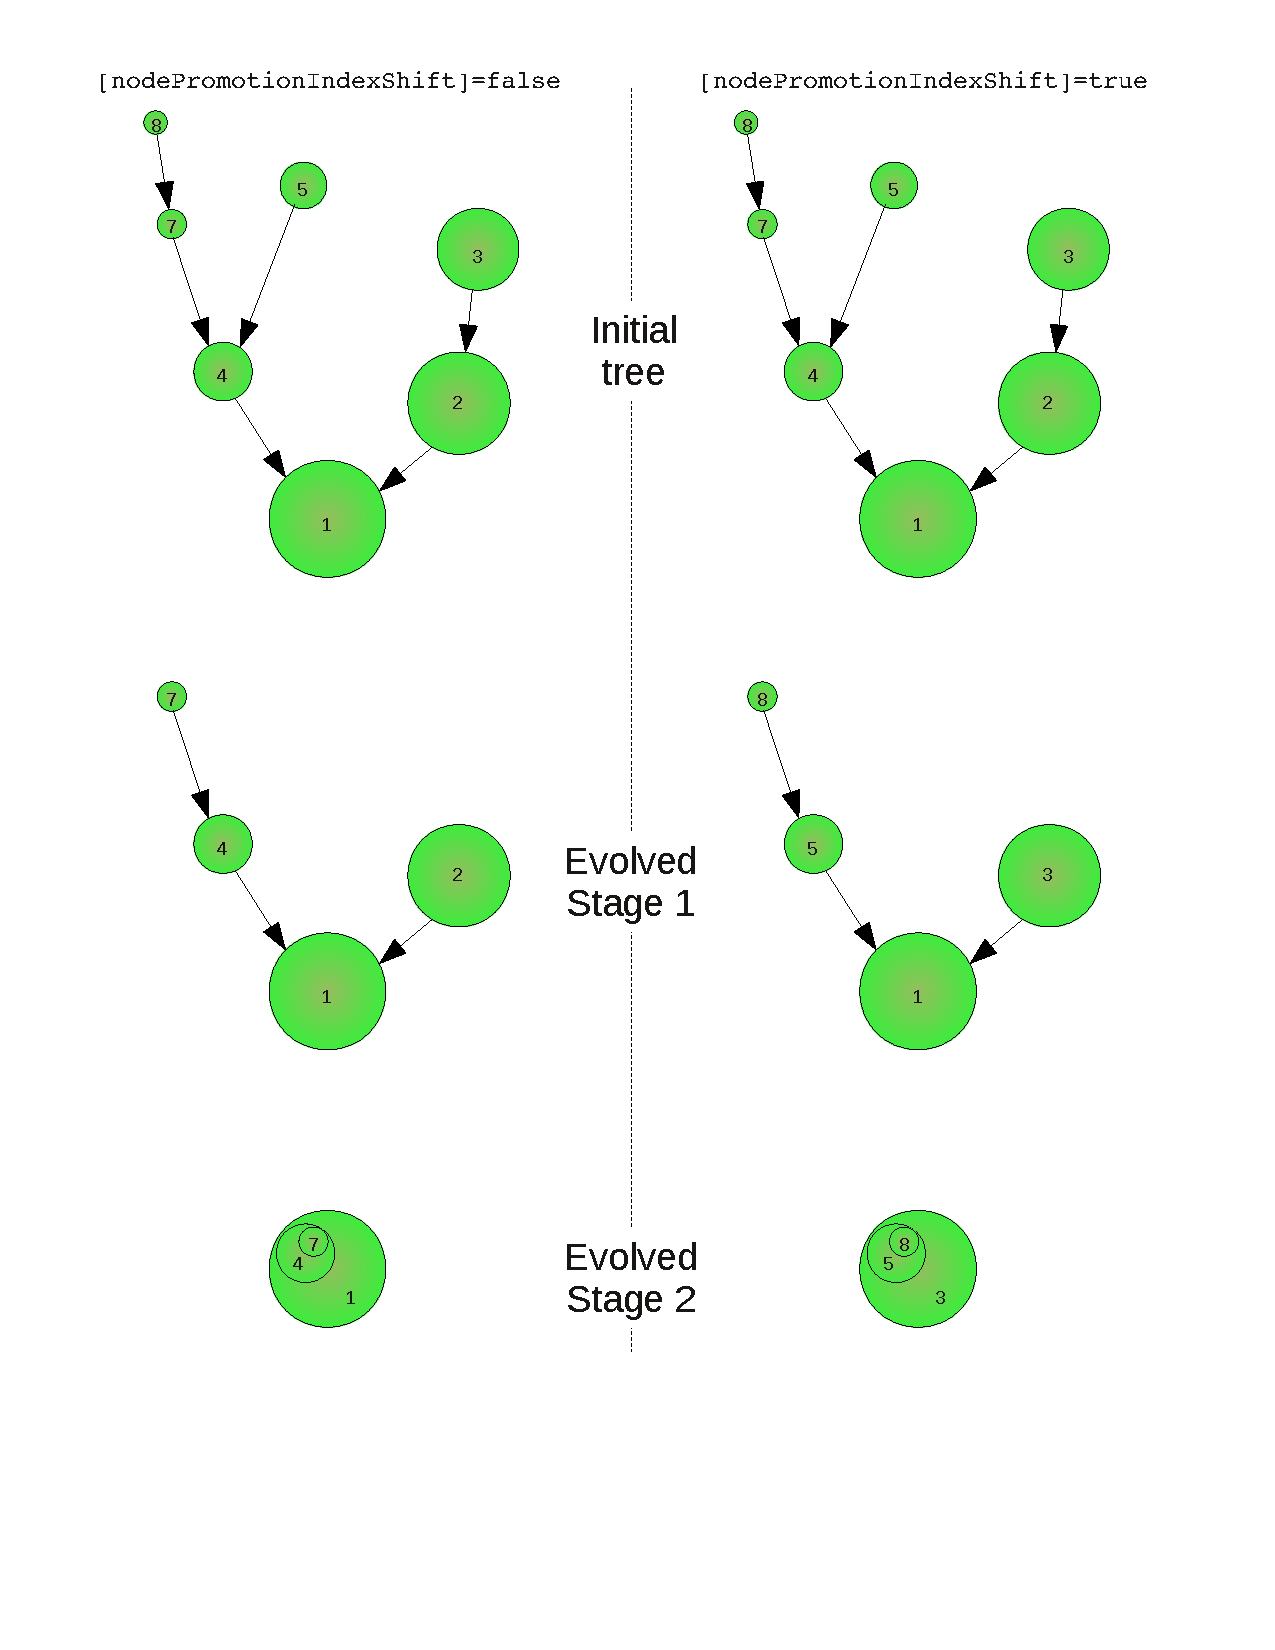
\includegraphics[width=140mm]{Diagrams/NodePromotionIndices.pdf}
 \end{center}
 \caption{Illustration of options for the propagation of node indices during node promotion events. Two identical trees (top row) are evolved with {\tt [nodePromotionIndexShift]}$=${\tt false} (left column) and {\tt [nodePromotionIndexShift]}$=${\tt true} (right column). The middle and lower rows indicate the resulting node indices after two stages of tree evolution.}
 \label{fig:NodePromotionIndexAlgorithms}
\end{figure}

\section{Merger Tree Data for Rendering}\index{merger tree!rendering}

Data on the structure of a merger tree and its halos useful for rendering the tree as a 3-D structure can be output using the \hyperlink{merger_trees.render.F90:merger_trees_render}{\tt Merger\_Trees\_Render} module. Calling \hyperlink{merger_trees.render.F90:merger_trees_render:merger_trees_render_dump}{\tt Merger\_Trees\_Render\_Dump} with a tree as the only argument will cause the tree structure will be dumped to a file named {\tt render\_$\langle$treeIndex$\rangle$\_$\langle$outputIndex$\rangle$.hdf5} where $\langle${\tt treeIndex}$\rangle$ is the index of the tree and $\langle${\tt outputIndex}$\rangle$ is an incremental counter that tracks the number of outputs for this tree. The output is a simple HDF5 file containing the following datasets:
\begin{description}
 \item [{\tt nodeIndex}] Index of the node;
 \item [{\tt parentIndex}] Index of the parent node;
 \item [{\tt childIndex}] Index of the child node;
 \item [{\tt time}] Time of the node;
 \item [{\tt expansionFactor}] Corresponding expansion factor;
 \item [{\tt radiusVirial}] Virial radius of the node;
 \item [{\tt position}] $(x,y,z)$ position of the node.
\end{description}

\section{Merger Tree Structure}\index{merger tree!structure}

The structure of each merger tree can optionally be dumped to a file suitable for post-processing with \href{http://www.graphviz.org/}{\sc dot} after every step of evolution. To request this output set {\tt [mergerTreesDumpStructure]}$=${\tt true}. After each evolution step the tree structure will be dumped to a file named {\tt mergerTreeDump:$\langle$treeIndex$\rangle$:$\langle$outputIndex$\rangle$.gv} where $\langle${\tt treeIndex}$\rangle$ is the index of the tree and $\langle${\tt outputIndex}$\rangle$ is an incremental counter that tracks the number of outputs for this tree. These files can be processed with \href{http://www.graphviz.org/}{\sc dot} to produce a diagram of the tree structure. The node currently being evolved will be highlighted in green. This output option makes use of the \hyperlink{objects.merger_trees.dump.F90:merger_trees_dump}{\tt Merger\_Trees\_Dump} module to create the outputs.

\section{Most Massive Progenitor}

Setting {\tt [outputMostMassiveProgenitor]}$=${\tt true} causes the property {\tt isMostMassiveProgenitor} to be output. This propert will be $1$ for the most massive progenitor node in a tree at each output time and $0$ for all other nodes.

\section{Star Formation Rates}\index{star formation rate!outputting}\index{outputs!star formation rate}

By default the star formation rate in each galaxy is \emph{not} output. However, setting {\tt [diskOutputStarFormationRate]} to true will cause the current star formation rate in the disk of each galaxy to be output as {\tt diskStarFormationRate} (in units of $M_\odot$/Gyr). The {\tt [spheroidOutputStarFormationRate]} has the same effect for the spheroid component.

\section{Virial Quantities}\index{virial}

The following quantities related to the virialized region of each node are output if {\tt outputVirialData} is set to true:
\begin{description}
 \item [{\tt nodeVirialRadius}] The virial radius (following whatever definition of virial overdensity was selected in \glc) in units of Mpc;
 \item [{\tt nodeVirialVelocity}] The circular velocity at the virial radius (in km/s).
\end{description}


\part{Development}

In this Part we focus on how to modify \glc\ to meet your own needs. \glc\ is designed in a modular way to make it as simple as possible to introduce new implementations of physical processes or new galactic components without breaking the rest of the code. Nevertheless, some understanding of the structure of the code is necessary. In particular, \glc\ will happily compile and run calculations that make no physical sense whatsoever---it's up to you to ensure that the changes you make are physically reasonable and consistent with the behavior of the rest of the code.

\chapter{Developing \glc}

The following is a quickstart guide to making changes to the \glc\ source code and contributing them back to the project. Note that the preferred method to do this is through \href{https://bitbucket.org}{\normalfont \scshape BitBucket}.

\section{Getting Started}

It's easy to begin working with and changing the \glc\ source code. Assuming you have Mercurial (``{\normalfont \ttfamily hg}'') installed, just do:
\begin{verbatim}
 hg clone https://abensonca@bitbucket.org/galacticusdev/galacticus galacticus
\end{verbatim}
and you have a cloned copy of the \glc\ repository in the {\normalfont \ttfamily galacticus} directory.

\subsection{Using {\normalfont \scshape BitBucket}}

If you plan to contribute changes back to the \glc] project (please do!), you should consider using \href{https://bitbucket.org}{\normalfont \scshape BitBucket}. After you've created an account for yourself at {\normalfont \scshape BitBucket}, you can ``fork'' the \glc\ repository to have your own working copy. This can be done as follows:
\begin{itemize}
 \item visit the \glc\ repository on {\normalfont \ttfamily BitBucket} at \href{https://bitbucket.org/galacticusdev/galacticus/overview}{\normalfont \ttfamily https://bitbucket.org/abensonca/galacticus/overview};
 \item click on the ``Fork'' button---you'll be presented with a form;
 \item fill out the form (setting a name for your fork, a short description, etc.), then click the ``Fork repository'' button;
 \item after the fork completes, you'll be taken to the overview page for your forked repository.
\end{itemize}. 

You'll now want to clone this forked repository to your local system. Click on the ``Clone'' button and copy the {\normalfont \ttfamily hg clone} command presented there (you want the {\normalfont \ttfamily SSH} version so that you can push changes back to this repository). Run this command on your local system to get a cloned copy of your new repository. You can now work with this repository, make any changes, and commit then. We'll discuss how to send these changes back to {\normalfont \scshape BitBucket}, and back to the \glc\ project below.

\section{Making Simple Changes}

If you want to make some relatively minor changes to the \glc\ code, such as fixing a typo, adding a new filter, etc. you can just make changes directly on the {\normalfont \ttfamily default} branch (i.e. at the point of active development). To do this, make sure you're at {\normalfont \ttfamily default}:
\begin{verbatim}
 hg pull
 hg update default
\end{verbatim}
Then make your changes, add new files, etc. Once you're done, first check if there have been any changes to {\normalfont \ttfamily default} since you {\normalfont \ttfamily pull}ed:
\begin{verbatim}
 hg incoming
\end{verbatim}
If any new changesets are shown, us {\normalfont \ttfamily hg pull -u} to merge these in to your working copy. Then commit your changes:
\begin{verbatim}
 hg commit
\end{verbatim}
Your changes are now commited to your cloned repository.

\subsection{Contributing Your Changes Back To \glc}

Once you've committed your changes, you can contribute them back to the \glc\ project.

\subsubsection{Via E-mail}

If you just cloned the \glc\ repository directly you can send a patch containing your changes by e-mail to \href{mailto:abenson@carnegiescience.edu}{abenson{@}carnegiescience.edu}. First, create the patch file using:
\begin{verbatim}
 hg export -r begin:end > changes.diff
\end{verbatim}
where {\normalfont \ttfamily begin} and {\normalfont \ttfamily end} are the first and last revisions that you want to include (you can specify more complicated sets of revisions of course). Then simply attached the {\normalfont \ttfamily changes.diff} file to an e-mail. It will be merged into the \glc\ project using
\begin{verbatim}
 hg import changes.diff
\end{verbatim}

\subsubsection{Using {\normalfont \scshape BitBucket}}

If you forked the \glc\ repository on {\normalfont \scshape BitBucket}, you can now push your changes back to {\normalfont \ttfamily BitBucket} using
\begin{verbatim}
 hg push
\end{verbatim}
If you want to contribute these changes back to the \glc\ project the best way to do so is to create a ``pull request''. Simply visit your forked respository on {\normalfont \scshape BitBucket} and click the ``Pull request'' button. The form you're presented with allows you to choose which branch in your respository you want to send changes from, and which branch in the \glc\ project you want them contributed to. Add a title and description of your changes (and, optionally, check the ``Close branch'' box if you're done with this branch of development) then click ``Create pull request''. Assuming your code looks godo and works, it can then be pulled into the \glc\ project.

\section{Making Bigger Changes}

For bigger changes, particularly those where you're adding a new feature, we recommend using Mercurial's ``feature branches''. These provide a permanent record of for which feature each changeset was added. Using feature branches is straightforward. Begin with {\normalfont \ttfamily default} and create a new branch:
\begin{verbatim}
 hg update default
 hg branch myNewFeature
\end{verbatim}
where {\normalfont \ttfamily myNewFeature} is a name for your feature branch. Then begin working, make changes, add new files etc. You can make commits when necessary (and it's good to make several small commits rather than one big one). You should merge {\normalfont \ttfamily default} into your feature branch as often as possible to avoid them getting out of sync (which makes for difficulty later when you want to merge your feature branch back into {\normalfont \ttfamily default}):
\begin{verbatim}
 hg update myFeatureBranch
 hg merge default
 hg commit -m "merged default into myFeatureBranch"
\end{verbatim}
Once the feature branch is stable, you can merge it back into {\normalfont \ttfamily default}:
\begin{verbatim}
 hg update default
 hg merge myFeatureBranch
 hg commit -m "merged myFeatureBranch"
\end{verbatim}
Once you're done developing this feature, you should close the feature branch:
\begin{verbatim}
 hg commit --close-branch -m "finished my feature"
\end{verbatim}
Note that you can always go back and work on a feature branch later, after you have closed it. Just do:
\begin{verbatim}
 hg up myFeatureBranch
 hg merge default
 hg commit -m "merged default into myFeatureBranch"
\end{verbatim}
then continue to work with your feature branch as normal (don't forget to close it again when you're finished working with it).

\section{Releases}

Each release of \glc\ exists as a separate branch within the main \glc\ repository. To work with a particular release use
\begin{verbatim}
 hg update v0.9.2
\end{verbatim}
replacing the version number with whichever version you want. To get back to the development tip use
\begin{verbatim}
 hg update default
\end{verbatim}

\subsection{Bug Fixes In Releases}

To make a bugfix in a release, simply {\normalfont \ttfamily hg update} to that release, fix the bug, and commit your changes. In many cases you'll want to fix the same bug in later releases and also in {\normalfont \ttfamily default}. To do that, just {\normalfont \ttfamily hg update} to each branch in turn, use {\normalfont \ttfamily hg merge fixedBranch} (where ``{\normalfont \ttfamily fixedBranch}'' is the name of the branch in which you fixed the branch, and then commit the merge. Once the bug has been fixed you can contribute the fix back to the \glc\ project using the methods described above.

\section{The \glc\ Build System}

\glc\ use a GNU Make-based build system. Dependencies are automatically discovered, and extensive meta-programming and preprocessing of source files is undertaken as part of the build. As a result, the build system is complicated. In this section the build system is described and detailed.

\subsection{The Makefile}

Files generated during the build (with the exception of final executables) are written to the directory specified by the {\normalfont \ttfamily BUILDPATH} environment variable. This is normally {\normalfont \ttfamily work/build/} (and is set by the {\normalfont \ttfamily Makefile}) unless a special build configuration is requested.

\subsection{Automatic Discovery}

Interdependencies between source files, together with requirements for auto-generated code are automatically discovered during the build process by processing of source files. All such automatic discovery is described below.

\subsubsection{Code Directive Parsing}\label{sec:buildDiscoveryDirectives}

The modular nature of \glc\ is enabled through the use of directives embedded within the source code (XML documents embedded as comment lines starting with a special tag) which instruct the build system how to link together the various functions. Parsing of these directives is handled by the {\normalfont \ttfamily codeDirectivesParse.pl}\index{codeDirectivesParse.pl@{\normalfont \ttfamily codeDirectivesParse.pl}} script.

For {\normalfont \ttfamily include} directives (which generate files that get included into the source), the script generates {\normalfont \ttfamily \$(BUILDPATH)/*.xml} files which describe the directive, and {\normalfont \ttfamily \$(BUILDPATH)/Makefile\_Directives} which contains rules for building those include files.

The script also outputs a file {\normalfont \ttfamily \$(BUILDPATH)/directiveLocations.xml} which provides list of files that contain each directive. This is used by other scripts to permit rapid processing of files associated with each directive.

\subsubsection{Allocatable Arrays}\label{sec:buildDiscoverAllocatables}

Types and ranks of allocatable arrays required by the \glc\ are discovered by the {\normalfont \ttfamily allocatableArrays.pl}\index{allocatableArrays.pl@{\normalfont \ttfamily allocatableArrays.pl}} script. Source files are parsed for dimensionful, allocatable intrinsic types. All such combinations of type and rank are stored to a file {\normalfont \ttfamily \$(BUILDPATH)/allocatableArrays.xml}. The content of this file is later used to build appropriate memory allocation and deallocation functions (see \S\ref{sec:buildGenerationMemory}).

\subsubsection{Executable Files}\index{files!executable}\index{executable files}\label{sec:buildExecutables}

Files which produce executables (including the {\normalfont \ttfamily Galacticus.exe} executable) are discovered by the {\normalfont \ttfamily scripts/build/findExecutables.pl}\index{findExecutables.pl@{\normalfont \ttfamily findExecutables.pl}} script, which generates rules describing how these files should be built, along with all of their dependencies, and writes them to {\normalfont \ttfamily \$(BUILDPATH)/Makefile\_All\_Execs}\index{Makefile_All_Execs@{\normalfont \ttfamily Makefile\_All\_Execs}}. All Fortran files in the {\normalfont \ttfamily source} directory are parsed, and executable files are identified as those containing a {\normalfont \ttfamily program} statement. All executables so identified are also added to the list of objects that will be built by {\normalfont \ttfamily make all}.

\subsubsection{Modules Provided}\index{modules!provided}\index{provided modules}\label{sec:buildModulesProvided}

Determination of which files provide which Fortran modules is carried out by the {\normalfont \ttfamily scripts/build/moduleDependencies.pl}\index{moduleDependencies.pl@{\normalfont \ttfamily moduleDependencies.pl}} script, which generates rules describing these dependencies (and how to build the module file by compiling the corresponding source file) and writes them to {\normalfont \ttfamily \$(BUILDPATH)/Makefile\_Module\_Dependencies}\index{Makefile_Module_Dependencies@{\normalfont \ttfamily Makefile\_Module\_Dependencies}}.

Additionally, rules are generated which describe how to build the following classes of file:
\begin{description}
\item[{\normalfont \ttfamily *.mod.d}] Contains a list of all object files upon which the module depends. Used in constructing the final set of objects which must be linked to build an executable.
\item[{\normalfont \ttfamily *.mod.gv}] Contains a list of all source files upon which the module depends. Used in constructing \gls{graphviz} visualizations of dependencies.
\item[{\normalfont \ttfamily *.m}] Contains a list of all modules provided by the corresponding object file. Used when building object files to test whether corresponding module files have been changed---allows avoidance of recompilation cascades if modules do not need to be updated (i.e. if the modules do not differ as judged by the {\normalfont \ttfamily scripts/build/compareModules.pl}\index{findExecutables.pl@{\normalfont \ttfamily compareModules.pl}} script).
\end{description}

\subsubsection{Modules Used}\index{modules!used}\index{used modules}\label{sec:buildModulesUsed}

Determination of which files use which Fortran modules is carried out by the {\normalfont \ttfamily scripts/build/useDependencies.pl}\index{useDependencies.pl@{\normalfont \ttfamily useDependencies.pl}} script, which generates rules describing these dependencies and writes them to {\normalfont \ttfamily \$(BUILDPATH)/Makefile\_Use\_Dependencies}\index{Makefile_Use_Dependencies@{\normalfont \ttfamily Makefile\_Use\_Dependencies}}.

Additionally, rules are generated which describe how to build the following classes of file:
\begin{description}
\item[{\normalfont \ttfamily *.d}] Contains a list of all object files upon which each object file depends. Used in constructing the final set of objects which must be linked to build an executable.
\item[{\normalfont \ttfamily *.gv}] Contains a list of all source files upon which each file depends by virtue of {\normalfont \ttfamily use} statements. Used in constructing \gls{graphviz} visualizations of dependencies.
\item[{\normalfont \ttfamily *.fl}] Contains a list of libraries upon which each object file depends. Used in constructing the final set of libraries which must be linked with the executable.
\end{description}

\subsubsection{Included Files}\index{files!include}\index{include files}\label{sec:buildIncludeDeps}

Dependencies on files due to the use of ``{\normalfont \ttfamily include}'' statements (in both Fortran and C source files) are discovered by the {\normalfont \ttfamily scripts/build/includeDependencies.pl}\index{includeDependencies.pl@{\normalfont \ttfamily includeDependencies.pl}} script, which generates rules describing these dependencies and writes them to {\normalfont \ttfamily \$(BUILDPATH)/Makefile\_Include\_Dependencies}\index{Makefile_Include_Dependencies@{\normalfont \ttfamily Makefile\_Include\_Dependencies}}.

All Fortran and C/C++ source files in the {\normalfont \ttfamily source} directory are parsed. Files specified in any include statement in a source file are added as a dependency of that source file if unless the source file is C/C++ and the named include file can be found in either {\normalfont \ttfamily source/}, a standard system include path, or in any include path specified in the {\normalfont \ttfamily GALACTICUS\_CFLAGS}\index{environment variables!GALACTICUS_CFLAGS@{\normalfont \ttfamily GALACTICUS\_CFLAGS}}\index{GALACTICUS_CFLAGS@{\normalfont \ttfamily GALACTICUS\_CFLAGS}} or {\normalfont \ttfamily GALACTICUS\_CPPFLAGS}\index{environment variables!GALACTICUS_CPPFLAGS@{\normalfont \ttfamily GALACTICUS\_CPPFLAGS}}\index{GALACTICUS_CPPFLAGS@{\normalfont \ttfamily GALACTICUS\_CPPFLAGS}} environment variables.

\subsubsection{Parameter Dependencies}\index{parameters!dependencies}\label{sec:parameterDependencies}

All runtime parameters upon which a given executable may depend are discovered by the {\normalfont \ttfamily scripts/build/parameterDependencies.pl}\index{parameterDependencies.pl@{\normalfont \ttfamily parameterDependencies.pl}} script, which generates XML files listing these parameters and writes them to {\normalfont \ttfamily \$(BUILDPATH)/\textless executableName\textgreater.parameters.xml}\index{*.parameters.xml@{\normalfont \ttfamily *.parameters.xml}}. All Fortran and C++ files in the {\normalfont \ttfamily source} directory are parsed, and embedded parameter definitions (i.e. embedded XML blocks in lines beginning ``!\@'' for Fortran or ``//\@'' for C++ with root element {\normalfont \ttfamily inputParameter}) are identified. Any files included into a source file are also searched. In the case of Fortran source files, {\normalfont \ttfamily source/*.F90}, the corresponding preprocessed file, {\normalfont \ttfamily \$(BUILDPATH)/*.p.F90}, will be searched for parameter dependencies.

\subsection{Code Generation}

During build, code is generated automatically. Much of this is to link together functions within \glc\ (thereby permitting the modular nature of \glc), but also includes generation of various utility functions. All code generation is described below.

\subsubsection{Memory Management Functions}\label{sec:buildGenerationMemory}

Functions for allocation and deallocation of intrinsic-type arrays are generated by the {\normalfont \ttfamily memoryManagementFunctions.pl}\index{memoryManagementFunctions.pl@{\normalfont \ttfamily memoryManagementFunctions.pl}} script. Utilizing the list of such types in the {\normalfont \ttfamily \$(BUILDPATH)/allocatableArrays.xml} file (see \S\ref{sec:buildDiscoverAllocatables}) overloaded functions are created for each type. These memory management functions keep track of the total amount of memory allocated.

{\normalfont \ttfamily memoryManagementFunctions.pl}\index{memoryManagementFunctions.pl@{\normalfont \ttfamily memoryManagementFunctions.pl}}
 
\subsubsection{Directives}\label{sec:codeBuildIncludeDirectives}

Generation of code to implement the functionality of {\normalfont \ttfamily include} directives is carried out by the {\normalfont \ttfamily buildCode.pl}\index{buildCode.pl@{\normalfont \ttfamily buildCode.pl}} script. This script simply reads an XML file generated by the {\normalfont \ttfamily codeDirectivesParse.pl} (see \S\ref{sec:buildDiscoveryDirectives}), calls the appropriate function to generate the necessary code, passes this through the preprocessor (see \S\ref{sec:sourceTreePreprocessor}), and outputs the result to the appropriate include file.

\subsubsection{Pre- and Post-processing}\label{sec:codeBuildPrePostProcess}

Before being compiled, all Fortran source files are passed through a tree-based preprocessor. The functionality of this preprocessor is described in \S\ref{sec:sourceTreePreprocessor}. The preprocessor is invoked on each source file by the {\normalfont \ttfamily preprocess.pl}\index{preprocess.pl@{\normalfont \ttfamily preprocess.pl}} script, which takes a {\normalfont \ttfamily source/*.F90} file as input and outputs a preprocessed file {\normalfont \ttfamily \$(BUILDPATH)/*.p.F90}.

Output from the {\normalfont \ttfamily gfortran} compiler is directed through the {\normalfont \ttfamily postprocess.pl}\index{postprocess.pl@{\normalfont \ttfamily postprocess.pl}} script. This script currently performs the following functions:
\begin{itemize}
\item Builds a map from line numbers in the preprocessed source file back to line numbers in the unpreprocessed source, and translates line numbers in any error or warnings messages from the compiler into line numbers in the unpreprocessed source;
\item Filters out incorrect warning messages about the lack of scalar finalizers (see GCC \href{https://gcc.gnu.org/bugzilla/show_bug.cgi?id=58175}{PR58175});
\item Checks for unused function attributes in the source and filters out warnings about these unused functions.
\end{itemize}

\subsection{Build Files}

All files involved in the build process are summarized below.

\begin{description}

\item[{\normalfont \ttfamily scripts/build/allocatableArrays.pl}\index{allocatableArrays.pl@{\normalfont \ttfamily allocatableArrays.pl}}:] Discovers dimensionful, allocatable, intrinsic-typed arrays in the source code, and generates a summary of their types and ranks to the file {\normalfont \ttfamily \$(BUILDPATH)/allocatableArrays.xml} (see \S\ref{sec:buildDiscoverAllocatables});
  
\item[{\normalfont \ttfamily scripts/build/buildCode.pl}\index{buildCode.pl@{\normalfont \ttfamily buildCode.pl}}:] Acts upon {\normalfont \ttfamily include} directives embedded in the source code and generates the corresponding include file (see \S\ref{sec:codeBuildIncludeDirectives});

\item[{\normalfont \ttfamily scripts/build/codeDirectivesParse.pl}\index{codeDirectivesParse.pl@{\normalfont \ttfamily codeDirectivesParse.pl}}:] Discovers and parses directives embedded in source files. Generates {\normalfont \ttfamily make} rules for the resulting dependencies, a file providing a mapping of which files contain each directive, and rule files describing how to build each include file resulting from a {\normalfont \ttfamily include} directive;

\item[{\normalfont \ttfamily scripts/build/compareModuleFiles.pl}\index{compareModuleFiles.pl@{\normalfont \ttfamily compareModuleFiles.pl}}:] Tests whether two Fortran module files are identical (ignoring timestamp information). Used to avoid updating modules when not necessary and so avoids recompilation cascades;

\item[{\normalfont \ttfamily scripts/build/includeDependencies.pl}\index{includeDependencies.pl@{\normalfont \ttfamily includeDependencies.pl}}:] Discovers (and generates rules for) dependencies between files arising from the use of ``{\normalfont \ttfamily include}'' statements (see \S\ref{sec:buildIncludeDeps});
  
\item[{\normalfont \ttfamily \normalfont \ttfamily scripts/build/executableSize.pl\index{executableSize.pl@{\normalfont \ttfamily executableSize.pl}}}:] Generates a file containing details of the size of each generated executable which can be used at runtime for memory reporting (see \S\ref{sec:buildExecutables});

\item[{\normalfont \ttfamily \normalfont \ttfamily scripts/build/findExecutables.pl\index{findExecutables.pl@{\normalfont \ttfamily findExecutables.pl}}}:] Discovers (and generates rules for) files which generate executables (see \S\ref{sec:buildExecutables});

\item[{\normalfont \ttfamily scripts/build/libraryDependencies.pl}\index{libraryDependencies.pl@{\normalfont \ttfamily libraryDependencies.pl}}:] Determines the set of libraries that must be linked with each executable, and ensures they are ordered correctly for static linking;

\item[{\normalfont \ttfamily scripts/build/memoryManagementFunctions.pl}\index{memoryManagementFunctions.pl@{\normalfont \ttfamily memoryManagementFunctions.pl}}:] Generates memory allocation/deallocation functions for allocatable intrinsic arrays (see \S\ref{sec:buildGenerationMemory});

\item[{\normalfont \ttfamily scripts/build/moduleDependencies.pl}\index{moduleDependencies.pl@{\normalfont \ttfamily moduleDependencies.pl}}:] Discovers (and generates rules for) dependencies of module files on their source file statements (see \S\ref{sec:buildModulesProvided});

\item[{\normalfont \ttfamily scripts/build/parameterDependencies.pl}\index{parameterDependencies.pl@{\normalfont \ttfamily parameterDependencies.pl}}:] Determines all parameters upon which a given executable depends (see \S\ref{sec:parameterDependencies});

\item[{\normalfont \ttfamily scripts/build/postprocess.pl}\index{postprocess.pl@{\normalfont \ttfamily postprocess.pl}}:] Postprocesses the output of the {\normalfont \ttfamily gfortran} compiler to remove spurious warnings and provide line numbers in warning/error reports that point into the unpreprocessed source files (see \S\ref{sec:codeBuildPrePostProcess});

\item[{\normalfont \ttfamily scripts/build/preprocess.pl}\index{preprocess.pl@{\normalfont \ttfamily preprocess.pl}}:] Preprocesses Fortran source code to provide various extended functionality (see \S\ref{sec:codeBuildPrePostProcess});

\item[{\normalfont \ttfamily scripts/build/useDependencies.pl}\index{useDependencies.pl@{\normalfont \ttfamily useDependencies.pl}}:] Discovers (and generates rules for) dependencies between files originating from module {\normalfont \ttfamily use} statements (see \S\ref{sec:buildModulesUsed});
  
\item[{\normalfont \ttfamily \$(BUILDPATH)/Makefile\_All\_Execs}\index{Makefile_All_Execs@{\normalfont \ttfamily Makefile\_All\_Execs}}:] Contains rules describing how to build the executable file for each distinct program---generated by {\normalfont \ttfamily scripts/build/findExecutables.pl}\index{findExecutables.pl@{\normalfont \ttfamily findExecutables.pl}} (see \S\ref{sec:buildExecutables});

\item[{\normalfont \ttfamily \$(BUILDPATH)/Makefile\_Component\_Includes}\index{Makefile_Component_Includes@{\normalfont \ttfamily Makefile\_Component\_Includes}}:] Describes dependencies on the {\normalfont \ttfamily nodeComponent} class hierarchy module on include files which implement specific functionality for individual node component implementations;
  
\item[{\normalfont \ttfamily \$(BUILDPATH)/Makefile\_Directives}\index{Makefile_Directives@{\normalfont \ttfamily Makefile\_Directives}}:] Describes rules for building include files for {\normalfont \ttfamily include} directives;

\item[{\normalfont \ttfamily \$(BUILDPATH)/Makefile\_Include\_Dependencies}\index{Makefile_Include_Dependencies@{\normalfont \ttfamily Makefile\_Include\_Dependencies}}:] Contains rules describing the dependencies of source file on files included via ``{\normalfont \ttfamily include}'' statements---generated by {\normalfont \ttfamily scripts/build/includeDependencies.pl}\index{includeDependencies.pl@{\normalfont \ttfamily includeDependencies.pl}} (see \S\ref{sec:buildIncludeDeps});

\item[{\normalfont \ttfamily \$(BUILDPATH)/Makefile\_Module\_Dependencies}\index{Makefile_Module_Dependencies@{\normalfont \ttfamily Makefile\_Module\_Dependencies}}:] Contains rules which describe how to build module files from their source files (see \S\ref{sec:buildModulesProvided});

\item[{\normalfont \ttfamily \$(BUILDPATH)/Makefile\_Use\_Dependencies}\index{Makefile_Use_Dependencies@{\normalfont \ttfamily Makefile\_Use\_Dependencies}}:] Contains rules which describe dependencies between source file originating from module {\normalfont \ttfamily use} statements (see \S\ref{sec:buildModulesUsed});

\item[{\normalfont \ttfamily \$(BUILDPATH)/allocatableArrays.xml}\index{allocatableArrays.xml files@{\normalfont \ttfamily allocatableArrays.xml} files}:] Contains a summary of the types and ranks of dimensionful, allocatable, intrinsic-type arrays for which memory allocation/deallocation functions will be generated (see \S\ref{sec:buildDiscoverAllocatables});

\item[{\normalfont \ttfamily \$(BUILDPATH)/directiveLocations.xml}\index{directiveLocations.xml files@{\normalfont \ttfamily directiveLocations.xml} files}:] Contains a map of which files contain each code directive (see \S\ref{sec:buildDiscoveryDirectives});

\item[{\normalfont \ttfamily \$(BUILDPATH)/*.xml}\index{*.xml files@{\normalfont \ttfamily *.xml} files}:] Contain rules for building files for {\normalfont \ttfamily include} files (see \S\ref{sec:buildDiscoveryDirectives});

\item[{\normalfont \ttfamily \$(BUILDPATH)/*.d}\index{*.d files@{\normalfont \ttfamily *.d} files}:] Contain lists of dependencies on object files, and are accumulated to find the final set of files which must be linked to build each executable (see \S\ref{sec:buildModulesProvided} \& \S\ref{sec:buildModulesUsed});

\item[{\normalfont \ttfamily \$(BUILDPATH)/*.m}\index{*.m files@{\normalfont \ttfamily *.m} files}:] Contain lists of modules provided by each object file, and are used during testing whether modules have been updated (see \S\ref{sec:buildModulesProvided});

\item[{\normalfont \ttfamily \$(BUILDPATH)/*.fl}\index{*.fl files@{\normalfont \ttfamily *.fl} files}:] Contain lists of libraries upon which each object file dependes, and are used to determine the final set of libraries which must be linked with each executable (see \S\ref{sec:buildModulesUsed});

\item[{\normalfont \ttfamily \$(BUILDPATH)/*.gv}\index{*.gv files@{\normalfont \ttfamily *.gv} files}:] Contain lists of source files upon which each file depends and are used in the construction of \gls{graphviz} representations of file dependencies (see \S\ref{sec:buildModulesProvided} \& \S\ref{sec:buildModulesUsed});

\item[{\normalfont \ttfamily \$(BUILDPATH)/*.Inc}\index{*.Inc files@{\normalfont \ttfamily *.Inc} files}:] Unpreprocessed include files generated from {\normalfont \ttfamily include} dependencies (see \S\ref{sec:buildDiscoveryDirectives});

\item[{\normalfont \ttfamily \$(BUILDPATH)/*.inc}\index{*.inc files@{\normalfont \ttfamily *.inc} files}:] Preprocessed include files generated from {\normalfont \ttfamily include} dependencies (see \S\ref{sec:buildDiscoveryDirectives});

\item[{\normalfont \ttfamily \$(BUILDPATH)/*.p.F90}\index{*.p.F90 files@{\normalfont \ttfamily *.p.F90} files}:] Preprocessed Fortran source files (see \S\ref{sec:codeBuildPrePostProcess});

\item[{\normalfont \ttfamily \$(BUILDPATH)/*.parameters.xml}\index{*.parameters.xml files@{\normalfont \ttfamily *.parameters.xml} files}:] Contain lists of parameters upon which an executable depends (see \S\ref{sec:parameterDependencies});

\item[{\normalfont \ttfamily \$(BUILDPATH)/*.size}\index{*.size files@{\normalfont \ttfamily *.size} files}:] Contain the size of each executable file built, and are used at runtime for memory reporting purposes---generated by {\normalfont \ttfamily scripts/build/executableSize.pl}\index{executableSize.pl@{\normalfont \ttfamily executableSize.pl}} (see \S\ref{sec:buildExecutables}).
\end{description}


\chapter{Coding \glc}

\section{Node Class Hierarchy Builder}

The hierarchy of classes describing a merger tree node and its galaxy (i.e. {\normalfont \ttfamily treeNode}, {\normalfont \ttfamily nodeComponent}, {\normalfont \ttfamily nodeComponentBasic}, {\normalfont \ttfamily nodeComponentBasicStandard}, etc.) are built automatically to realize the set of component implementations and properties specified in source files.

\subsection{Variable Definitions}\label{sec:nodeBuilderVariableDefinitions}

Throughout the node objects builder code, Fortran variables are defined using a common specification. This is a simple hash containing the following entries:
\begin{description}
  \item[intrinsic] a string specifying the intrinsic Fortran type ({\normalfont \ttfamily integer}, {\normalfont \ttfamily logical}, {\normalfont \ttfamily real}, {\normalfont \ttfamily double precision}, {\normalfont \ttfamily complex}, {\normalfont \ttfamily double complex}, {\normalfont \ttfamily type}, {\normalfont \ttfamily class}, {\normalfont \ttfamily procedure});
  \item[type] \emph{[optional, except for {\normalfont \ttfamily type} and {\normalfont \ttfamily class} intrinsics]} a string specifying the type of the variables;
  \item[attributes] an array of strings specifying all attributes of the variables;
  \item[variables] an array of strings giving the names of the variables.
\end{description}
For example, rank-1, long integer arguments which will not be modified in their function would be specified as:
\begin{verbatim}
{
  intrinsic  => "integer", 
  type       => "kind_int8",
  attributes => [ "dimension(:)", "intent(in)" ],
  variables  => [ "argument1", "argument2" ]
}
\end{verbatim}

\subsection{The {\normalfont \ttfamily \$build} Data Structure}

The {\normalfont \ttfamily \$build} data structure is used to accumulate all objects, variables, interfaces, and functions needed to build the class hierarchy used to represent nodes and components in \glc. At the end of the node objects build process, this object is processed to generate the required Fortran code. The following subsections describe how to add information to this object.

\subsubsection{Component Classes and Implementations}

A reference to a hash of structures which define all component classes, keyed by class name, is provided as {\normalfont \ttfamily \$build->\{'componentClasses'\}}. Each component class structure has the form:
\begin{verbatim}
{
 name    => <name of the class>,
 members => <reference to a hash of structures which define all member implementation of the class>
}
\end{verbatim}
Each member implementation structure has the form:
\begin{verbatim}
{
 name       =>             <name of the implementation>,
 properties => property => <reference to a hash of structures which define all properties of this implementation>
}
\end{verbatim}

\subsubsection{Types}\label{sec:buildHierarchyTypes}

Definitions of derived types are accumulated to the hash {\normalfont \ttfamily \$build->\{'types'\}}, with the key of each entry being the derived type's name. Each derived type structure has the form:
\begin{verbatim}
{
 name           => <name of the derived type>
 comment        => <a description of the type>
 isPublic       => <1 if the class should have public visbility, 0 otherwise>
 dataContent    => <variable list containing all data for this class>
 boundFunctions => 
  [
   {
    type        => <procedure|generic>
    descriptor  => <a function descriptor data structure> [optional]
    name        => <name of the bound method>
    function    => <name of function to bind to> [optional; not required if descriptor is provided]
    description => <LaTeX-syntax description of the method> [optional; not required if descriptor is provided]
    returnType  => <LaTeX-syntax return type of the method> [optional; not required if descriptor is provided]
    arguments   => <LaTeX-syntax definition of all arguments to the method> [optional; not required if descriptor is provided]
   }
  ]
}
\end{verbatim}
The preferred approach is to provide a function descriptor (see \S\ref{sec:buildHierarchyFunctions}), and to omit the {\normalfont \ttfamily function}, {\normalfont \ttfamily description}, {\normalfont \ttfamily returnType}, and {\normalfont \ttfamily arguments} entries (which will be inferred from the function descriptor). The {\normalfont \ttfamily function}, {\normalfont \ttfamily description}, {\normalfont \ttfamily returnType}, and {\normalfont \ttfamily arguments} entries will eventually be deprecated in favor of the {\normalfont \ttfamily descriptor} entry.

\subsubsection{Interfaces}\label{sec:buildHierarchyInterfaces}

Definitions of interfaces are accumulated to the hash {\normalfont \ttfamily \$build->\{interfaces\}}, with the key of each entry being the interfaces name. Each interface structure has the form:
\begin{verbatim}
{
 name           => <name of the interface>
 comment        => <a description of the interface>
 intrinsic      => <the intrinsic type of the function (or "void" for a subroutine)> 
 data           => <variable list containing all arguments for this interface>
\end{verbatim}

\subsubsection{Functions}\label{sec:buildHierarchyFunctions}

Definitions of functions are accumulated either to the list {\normalfont \ttfamily \$build->\{'functions'\}} or are included as the {\normalfont \ttfamily descriptor} in a derived type structure (this is the preferred method for functions that \emph{are} bound to a derived type; see \S\ref{sec:buildHierarchyTypes}). Each function structure has the form:
\begin{verbatim}
{
 type        => <the type of function>
 name        => <function name>
 description => <LaTeX-syntax description of the function>
 modules     => <list of names of modules required by the function> [optional]
 variables   => <list of variables required by the function> [optional]
 content     => <the code of the function (excluding opener, closer, and variable definitions)>
}
\end{verbatim}

\subsubsection{Module-scope Variables}

Any module-scope variables can be pushed to the array {\normalfont \ttfamily \@\{\$build->\{'variables'\}\}}, using the usual definition format described in \S\ref{sec:nodeBuilderVariableDefinitions}.

\section{Galacticus Preprocessor Directives}\label{sec:sourceTreePreprocessor}

\glc\ has its own preprocessor for Fortran source files. This preprocesses parses each source file into an internal tree representation, performs various manipulations on that tree, and then outputs the preprocessed file for compilation. The preprocessor is used to automate and standardize many common tasks, through the inclusion of directives into the source code. Directives are specified in comment lines beginning {\normalfont \ttfamily !\#}, and are written in XML. The remainder of this section describes the various preprocessor functionalities, and gives examples of their usage.

\subsection{Source Code Introspection}

The source code introspection functionality allows automated generation of information about the source code. Specifically:
\begin{itemize}
\item The directive {\normalfont \ttfamily \{introspection:location\}} in source code will be replaced with a character string giving a backtrace of the current location in the code, including any function, module, and file (including line number).
\end{itemize}

\subsection{Function Attributes}

\glc\ allows the specification of attributes for functions which alter the way the compiler treats them. Function attributes are specified as:
\begin{verbatim}
!$GLC function attributes {attributes} :: {functionNames}
\end{verbatim}
where {\normalfont \ttfamily \{attributes\}} is a space-separated list of attributes, and {\normalfont \ttfamily \{functionNames\}} is a space-separated list of functions to apply these functions to. Function attribute directives may appear anywhere in a file containing the named function, but it is good practice to locate them immediately before the function.

Currently, the supported attributes are:
\begin{description}
\item[{\normalfont \ttfamily unused}] The function is marked as being \emph{possibly} unused. Compiler warnings about unused functions will be suppressed for this function.
\end{description}

\subsection{Source Digest}

The {\normalfont \ttfamily sourceDigest} directive will generate an \gls{MD5hash} hash of the source code of the file in which the directive is placed, along with the source code of any files upon which it depends. This can be useful in generating unique labels (e.g. to use as suffixes in file names) which automatically update if the source code is modified. To generate a source digest simply use:

\begin{lstlisting}
  !# <sourceDigest name="mySourceDigest"/>
\end{lstlisting}

A source digest will be generated and stored as a {\normalfont \ttfamily character(len=22)} variable called {\normalfont \ttfamily mySourceDigest}.

\subsection{Object Builder}

When constructing instances of a class from a provided parameter set, a common pattern is to need to construct other objects based on those parameters, which will be used by the instance. For example, a transfer function class might require a cosmological parameters object for its operation. In such cases, we often want to use the default instance of the required class unless a different instance is explicitly specified. The {\normalfont \ttfamily objectBuilder} directive automates this process.

As an example, the following constructor requires an instance of the {\normalfont \ttfamily cosmologyParameters} class, which is passes to an internal constructor:

\begin{lstlisting}  
  function myConstructorParameters(parameters)
    use Input_Parameters2
    implicit none
    type(myClass                  )                :: myConstructorParameters
    type(inputParameters          ), intent(in   ) :: parameters
    class(cosmologyParametersClass), pointer       :: cosmologyParameters_    

    !# <objectBuilder class="cosmologyParameters" name="cosmologyParameters_" source="parameters"/>
    myConstructorParameters=myConstructorInternal(cosmologyParameters_)
    return
  end function myConstructorParameters
\end{lstlisting}

The {\normalfont \ttfamily objectBuilder} directive will assign a member of the class specified by the {\normalfont \ttfamily class} attribute to the variable specified by the {\normalfont \ttfamily name} attribute. If the parameter set specified by the {\normalfont \ttfamily parameters} attribute contains an explicit definition of the relevant class, that definition will be used to construct the instance. Otherwise, the parent parameter set will be checked for a definition of the relevant class, and so on. If no definition is found when the root parameter set is found the default instance will be used. Note that objects created by an {\normalfont \ttfamily objectBuilder} directive are directly associated with the element in the input parameters XML document from which they were created. Therefore, if a later {\normalfont \ttfamily objectBuilder} requires the object from that same XML element, it will reuse the one previously created.

The {\normalfont \ttfamily objectBuilder} directive by default searches for a parameter named {\normalfont \ttfamily \{class\}} where {\normalfont \ttfamily \{class\}} is the value of the {\normalfont \ttfamily class} attribute in the directive. An alternative name may be specified via the addition of a {\normalfont \ttfamily parameterName} attribute.

In cases where an explicit {\normalfont \ttfamily parameterName} attribute is given, it is possible to specify an explicit default for the object if no such named parameter is found. (Where no explicit {\normalfont \ttfamily parameterName} attribute is given the global default of the class is used.) A default is specified by adding a {\normalfont \ttfamily default} element to the directive, which should contain default specification for the object (and any subobjects) in the usual format. For example:
\begin{verbatim}
 !# <objectBuilder class="massDistribution" parameterName="diskMassDistribution" name="diskMassDistribution" source="globalParameters">
 !#  <default>
 !#   <diskMassDistribution value="exponentialDisk">
 !#    <dimensionless value="true"/>
 !#   </diskMassDistribution>
 !#  </default>
 !# </objectBuilder>
\end{verbatim}

\subsection{Object Destructor}

This directive can (and should) be used to destroy objects built by the {\normalfont \ttfamily objectBuilder} directive. The {\normalfont \ttfamily objectDestructor} directive automates the process of deciding if these objects should be destroyed (or merely have pointers to them nullified). As an example, the following destructor destroys two associated objects:
\begin{lstlisting}  
  subroutine simpleDestructor(self)
    implicit none
    type(powerSpectrumPrimordialTransferredSimple), intent(inout) :: self

    !# <objectDestructor name="self%transferFunction_"       />
    !# <objectDestructor name="self%powerSpectrumPrimordial_"/>
   return
  end subroutine simpleDestructor
\end{lstlisting}

\subsection{Constructor Assignments}

A common requirement in object constructors is to assign the values of arguments to the constructor to corresponding entries in the object. The {\normalfont \ttfamily constructorAssign} directive performs this assignment for a list of comma-separated variables. For example:
\begin{lstlisting}  
 function stellarMassConstructorInternal(massThreshold)
    implicit none
    type            (galacticFilterStellarMass)                :: stellarMassConstructorInternal
    double precision                           , intent(in   ) :: massThreshold
    !# <constructorAssign variables="massThreshold"/>
    return
  end function stellarMassConstructorInternal
\end{lstlisting}
will cause the value of the {\normalfont \ttfamily massThreshold} argument to {\normalfont \ttfamily stellarMassConstructorInternal\%massThreshold}. If an argument name is prefixed with {\normalfont \ttfamily \textasteriskcentered} in the variables list, pointer assignment is used instead of standard assignment.

\subsection{State Storing}

\glc\ supports storing its internal state to file to allow \href{https://github.com/galacticusorg/galacticus/releases/download/bleeding-edge/Galacticus_Usage.pdf\#sec.Restarting}{restarts}. Code to store and restore the internal state of objects of a given class can be generated automatically through use of the {\normalfont \ttfamily stateStorable} directive. An example is:
\begin{verbatim}
 !# <stateStorable class="table">
 !#  <table1DGeneric>
 !#   <restoreTo variables="reset" state=".true."/>
 !#   <exclude variables="staticData"/>
 !#  </table1DGeneric>
 !#  <table2DLinLinLin>
 !#   <restoreTo variables="resetX, resetY" state=".true."/>
 !#  </table2DLinLinLin>  
 !# </stateStorable>
\end{verbatim}
This specifies that the {\normalfont \ttfamily table} class (and all child classes) can and should be stored to file as part of the representation of the internal state. Code to store and restore all data associated with any object of this class (as well as restoring polymorphic objects to the correct type) will be generated. If certain variables of the class or subclass should be restored to specific values this can be specified through a {\normalfont \ttfamily restoreTo} element placed within an element with the name of the class or subclass (e.g. the {\normalfont \ttfamily table1DGeneric} in the above example). The {\normalfont \ttfamily restoreTo} element should specify a comma-separated list of one or more variables to set in its {\normalfont \ttfamily variables} attribute, and the state to which they should be restored in its {\normalfont \ttfamily state} attribute. Any variables which should be excluded from state store/restore (e.g. if their values are known to be determined statically at construction) can be specified via a {\normalfont \ttfamily exclude} element---a list of variables to exclude should be given as a comma-separated list in its {\normalfont \ttfamily variables} attribute.

\subsection{Conditional Call}

In some instances it is useful to be able to call a function with different combinations of optional arguments depending on certain conditions. (For example, if some combinations of optional arguments are mutually exclusive.) This can be achieved using the {\normalfont \ttfamily conditionalCall} directive. An example is:
\begin{verbatim}
  !# <conditionalCall>
  !#  <call>self=massDistributionBetaProfile(beta{conditions})</call>
  !#  <argument name="densityNormalization" value="densityNormalization" parameterPresent="parameters"/>
  !#  <argument name="mass"                 value="mass"                 parameterPresent="parameters"/>
  !#  <argument name="outerRadius"          value="outerRadius"          parameterPresent="parameters"/>
  !#  <argument name="coreRadius"           value="coreRadius"           parameterPresent="parameters"/>
  !#  <argument name="dimensionless"        value="dimensionless"        parameterPresent="parameters"/>
  !# </conditionalCall>
  !# <inputParametersValidate source="parameters"/>
\end{verbatim}
The {\normalfont \ttfamily call} element specifies the function call, and contains the special sequence {\normalfont \ttfamily \{conditions\}} which will be replaced with the conditionally-present arguments. One or more {\normalfont \ttfamily argument} elements should specify the various arguments which should be included in the call. For each such element the {\normalfont \ttfamily name} attribute specifies the name of the dummy argument in the called function, the {\normalfont \ttfamily value} attribute specifies the value (or variables) to pass this this dummy argument. A condition for inclusion of the argument must also be specified. In the above, the special {\normalfont \ttfamily parameterPresent} condition is used. The argument will be included in the call if a parameter with a name matching the {\normalfont \ttfamily name} attribute exists in the parameter set named in the {\normalfont \ttfamily parameterPresent} attribute. Alternatively a {\normalfont \ttfamily condition} attribute can be given. An argument is included in the call if the expression given in the {\normalfont \ttfamily condition} attribute evaluates to true.

Code will be generated to call the function with all possible combinations of arguments.

\subsection{Optional Arguments}

Fortran supports optional arguments to functions, but does not provide for a default value if those arguments are not present. The {\normalfont \ttfamily optionalArgument} directive allows a default value to be specified. In the following example, a default value is defined for the {\normalfont \ttfamily units} argument:

\begin{lstlisting}
  double precision function simpleHubbleConstant(self,units)
    implicit none
    class  (cosmologyParametersSimple), intent(inout)           :: self
    integer                           , intent(in   ), optional :: units
    !# <optionalArgument name="units" defaultsTo="hubbleUnitsStandard" />

    select case (units_)
    case (hubbleUnitsStandard)
       ! Return the value using the default units.
    case ....
       ! Return the value using some other units.
    end select
    return
  end function simpleHubbleConstant
\end{lstlisting}
The {\normalfont \ttfamily optionalArgument} directive should appear after variable declarations and before any attempt to use the optional argument, and should have two attributes, {\normalfont \ttfamily name} and {\normalfont \ttfamily defaultsTo} which give the name of the argument variable and its default value respectively. The preprocessor will add a new variable with the same name plus an underscore suffix, and will ensure that it is initialized to the default value if the optional variable is not present, otherwise setting it to the value of the optional variable.

Note that for optional arguments that are {\normalfont \ttfamily intent(out)} or {\normalfont \ttfamily intent(inout)} the preprocessor currently \emph{does not} ensure that the value of the new variable is copied back to the argument prior to exit from the function.

\subsection{Enumerations}

The {\normalfont \ttfamily enumeration} directive allows specification of an enumeration (a set of labels), and (optionally) functions to decode such a label from user input. The following example illustrates this usage:

\begin{lstlisting}
module Cosmology_Parameters

  !# <enumeration>
  !#  <name>hubbleUnits</name>
  !#  <description>Specifies the units for the Hubble constant.</description>
  !#  <visibility>public</visbility>
  !#  <validator>yes</validator>
  !#  <encodeFunction>yes</encodeFunction>
  !#  <entry label="standard" />
  !#  <entry label="time"     />
  !#  <entry label="littleH"  />
  !# </enumeration>

contains

subroutine Test_Enumeration()
    use ISO_Varying_String
    implicit none
    class(cosmologyParametersClass), pointer :: cosmologyParameters_
    cosmologyParameters_ => cosmologyParameters()
    write (0,*) "Enumeration contains ",hubbleUnitsCount," entries from ",hubbleUnitsMin," to ",hubbleUnitsMax
    write (0,*) "Hubble constant in little-h units is: ",cosmologyParameters_%HubbleConstant(hubbleUnitsLittleH)
    if (enumerationHubbleUnitsEncode('hubbleUnitsStandard') == hubbleUnitsStandard) then
      write (0,*) "Enumeration decoding succeeded"
    else
      write (0,*) "Enumeration decoding failed"
    end if
    if (enumerationHubbleUnitsEncode('standard',includesPrefix=.false.) == hubbleUnitsStandard) then
      write (0,*) "Enumeration decoding succeeded"
    else
      write (0,*) "Enumeration decoding failed"
      end if
      write (0,*) "Name from time value is '",char(enumerationHubbleUnitsDecode(hubbleUnitsTime,includePrefix=.true.)),"'"
    return
  end subroutine Test_Enumeration

end module Cosmology_Parameters
\end{lstlisting}

Enumerations must be defined in the declaration section of a {\normalfont \ttfamily module}. The encoding and decoding functions will only be generated if the {\normalfont \ttfamily encode} element is present and has content {\normalfont \ttfamily yes}. The enumeration variables are given {\normalfont \ttfamily public} visibility by default---this can be overridden using the {\normalfont \ttfamily visibility} element. If the {\normalfont \ttfamily validator} element is present and set to {\normalfont \ttfamily yes} then a function is created which will return true if the given value is a valid one for the enumeration. Additionally, if the {\normalfont \ttfamily validator} element is present and set to {\normalfont \ttfamily yes} variables are created giving a count of the number of entries in the enumeration, along with the minimum and maximum values in the enumeration. Note that the {\normalfont \ttfamily description} element is used to generate an entry for the enumeration in the document, and so should be written in \LaTeX\ syntax.

\subsection{Input Parameters}

The {\normalfont \ttfamily inputParameter} directive reads an input parameter and assigns the appropriate value to the given variable. {\normalfont \ttfamily inputParameter} directives must occur within the main body of a function, subroutine, or program. A default value can be specified if desired. The following example illustrates this usage:

\begin{lstlisting}
  subroutine simpleParametersRead()
    implicit none
    double precision :: hubbleConstant
    !# <inputParameter>
    !#   <name>HubbleConstant</name>
    !#   <source>myParameters</source>
    !#   <variable>hubbleConstant</variable>
    !#   <defaultValue>69.7d0</defaultValue>
    !#   <defaultSource>(\citealt{hinshaw_nine-year_2012}; CMB$+H_0+$BAO)</defaultSource>
    !#   <description>The present day value of the Hubble parameter in units of km/s/Mpc.</description>
    !#   <type>real</type>
    !#   <cardinality>0..1</cardinality>
    !# </inputParameter>
    if (hubbleConstant < 0.0d0) write (0,*) "The universe is collapsing!"
    return
  end subroutine simpleParametersRead
\end{lstlisting}

In this case, the value of the {\normalfont \ttfamily HubbleConstant} parameter is assigned to the {\normalfont \ttfamily hubbleConstant} variable, with a default of $69.7$ if no value was specified in the input parameter file. If the {\normalfont \ttfamily source} element is present, the parameter will be read from the named {\normalfont \ttfamily inputParameters} set, otherwise the parameter will be read from the top-level of the parameters file. The {\normalfont \ttfamily defaultSource}, {\normalfont \ttfamily <description>The}, {\normalfont \ttfamily type}, and {\normalfont \ttfamily cardinality} elements are used only for adding an entry for the input parameter to the documentation, and so should be written in \LaTeX\ syntax.

It is also possible to specify a set of parameter which iterate over names defined by other directives. The following example would read one parameter named ``{\normalfont \ttfamily fileNameForXXXXXXIMF}'' where ``{\normalfont \ttfamily XXXXXX}'' equals the {\normalfont \ttfamily name} element each {\normalfont \ttfamily imfRegisterName} directive:
\begin{lstlisting}
    !# <inputParameter>
    !#   <iterator>fileNameFor(#imfRegisterName->name)IMF</iterator>
    !#   <source>parameters</source>
    !#   <variable>fileNames(IMF_Index("$1"))</variable>
    !#   <defaultValue>Galacticus_Input_Path()//"data/SSP_Spectra_imf$1.hdf5"</defaultValue>
    !#   <description>The name of the file of stellar populations to use for the named \gls{imf}.</description>
    !#   <type>string</type>
    !#   <cardinality>0..1</cardinality>
  !# </inputParameter>
\end{lstlisting}

\subsection{Input Parameter Lists}

The {\normalfont \ttfamily inputParameterList} directive will construct a {\normalfont \ttfamily varying\_string} array containing the names of all input parameters which are defined in the unit in which the directive appears. The name of the array is specified by the {\normalfont \ttfamily label} attribute of the {\normalfont \ttfamily inputParameterList} directive. If a {\normalfont \ttfamily source} attribute is specified in the directive then only parameters being read from the named variable will be included in the list, otherwise any parameters read will be included. Such a list can be used to validate the names of parameters passed to a function for example.

\subsection{Function Classes}

Most\footnote{At this time the \protect\glc\ code base is being transitioned to use this approach.} of the internal functionality within \glc\ is provided by ``function classes''. These are classes (in the object oriented sense) which model some particular physical entity or concept (e.g. the underlying cosmological model) and provide one or more functions associated with that entity or concept. A default implementation of each function class can be selected at run-time, allowing for simple user-defined control of model behavior. A function class is specified by a {\normalfont \ttfamily functionClass} directive, together with one or more implementations of the function class specified by their own directives.

An example of a function class directive, which defines a class for cosmological parameters (which in this case, for simplicity, consists of just the Hubble constant) is given below:

\begin{lstlisting}
  !# <functionClass>
  !#  <name>cosmologyParameters</name>
  !#  <descriptiveName>Cosmological Parameters</descriptiveName>
  !#  <description>Object providing various cosmological parameters.</description>
  !#  <default>simple</default>
  !#  <defaultThreadPrivate>no</defaultThreadPrivate>
  !#  <stateful>no</stateful>
  !#  <calculationReset>no</calculationReset>
  !#  <method name="HubbleConstant" >
  !#   <description>Return the Hubble constant at the present day. The optional {\normalfont \ttfamily units} argument specifies if the return value should be in units of km/s/Mpc (hubbleUnitsStandard), Gyr$^{-1}$ (hubbleUnitsTime), or 100 km/s/Mpc (hubbleUnitsLittleH).</description>
  !#   <type>double precision</type>
  !#   <pass>yes</pass>
  !#   <argument>integer, intent(in   ), optional :: units</argument>
  !#  </method>
  !# </functionClass>
\end{lstlisting}

The directive should contain the following elements:
\begin{description}
\item[{\normalfont \ttfamily name}] The name of this function class.
\item[{\normalfont \ttfamily descriptiveName}] A descriptive name for the function class, suitable for inclusion in the documentation.
\item[{\normalfont \ttfamily description}] A description of the purpose of this function class. This description will be included into the documentation so should be written in \LaTeX\ syntax.
\item[{\normalfont \ttfamily default}] The default implementation to use for this function class if no choice is made in the input parameter file.
\item[{\normalfont \ttfamily defaultThreadPrivate}] \emph{(optional)} If present and set to {\normalfont \ttfamily yes} then the default implementation of this function class will be made OpenMP thread private. Otherwise, the default implementation is shared between threads. A thread private default implementation can be useful if the function class may need to generate look-up tables unique to each thread on the fly for example.
\item[{\normalfont \ttfamily calculationReset}] \emph{(optional)} If present and set to {\normalfont \ttfamily yes} then the default implementation of the function class is assumed to possibly want to reset its calculations when the active \gls{node} changes (see \S\ref{sec:CalculationResetTask}). In this case, an additional method is generated for the function class: {\normalfont \ttfamily calculationReset} with interface:
  \begin{lstlisting}
    subroutine calculationReset(self,thisNode)
      class  (functionClassBaseName), intent(inout)          :: self
      type   (treeNode             ), intent(inout), pointer :: thisNode
    end subroutine calculationReset
  \end{lstlisting}
  This method has a null implementation for the base class of the function class, but can be overridden to reset calculations of any given implementation.
\item[{\normalfont \ttfamily method}] Each {\normalfont \ttfamily method} element defines a method which the function class will support, the name of which is given by a {\normalfont \ttfamily name} attribute. The method definition must contain the following elements:
  \begin{description}
  \item[{\normalfont \ttfamily description}] A description of this method (in \LaTeX\ syntax) suitable for inclusion into the documentation.
  \item[{\normalfont \ttfamily type}] The type of the function (e.g. {\normalfont \ttfamily double precision}; use {\normalfont \ttfamily void} for a subroutine).
  \item[{\normalfont \ttfamily pass}] If {\normalfont \ttfamily yes} pass the object that the method was called on as the first argument.
  \item[{\normalfont \ttfamily argument}] \emph{(optional)} Zero or more declarations (in standard Fortran syntax) for the method arguments (there is no need to specify the declaration for the object upon which the method was called in the case where this object is passed to the method function).
  \end{description}
\end{description}

Implementations of this function class must be declared with a directive having the same name as the function class (i.e. {\normalfont \ttfamily cosmologyParameters} in the example above). The directive must give the name of the implementation as an attribute, and a description of the implementation suitable for inclusion into the documentation. Each implementation should be placed in a separate file---the preprocessor will find these files and merge the implementations and function class definition into a single file for compilation. Each implementation should declare a class which extends the basic function class, constructor interfaces, and any module-scope data required by the class. The implementation should also define all necessary functions required by the class (separated from the declarations by a {\normalfont \ttfamily contains} keyword). An example is given below:

\begin{lstlisting}
  !# <cosmologyParameters name="cosmologyParametersSimple">
  !#  <description>Provides the Hubble constant: $H_0$.</description>
  !# </cosmologyParameters>
  type, extends(cosmologyParametersClass) :: cosmologyParametersSimple
     private
     double precision :: HubbleConstantValue
   contains
     final     ::                    simpleDestructor
     procedure :: HubbleConstant  => simpleHubbleConstant
  end type cosmologyParametersSimple

  interface cosmologyParametersSimple
     module procedure simpleDefaultConstructor
     module procedure simpleConstructor
  end interface cosmologyParametersSimple

contains

  function simpleDefaultConstructor()
    implicit none
    type(cosmologyParametersSimple) :: simpleDefaultConstructor

    ! Construct an instance of this class using a value of the Hubble constant read from the input parameter file.
    !# <inputParameter>
    !#   <name>H_0</name>
    !#   <variable>simpleDefaultConstructor%HubbleConstantValue</variable>
    !#   <defaultValue>69.7d0</defaultValue>
    !#   <defaultSource>(\citealt{hinshaw_nine-year_2012}; CMB$+H_0+$BAO)</defaultSource>
    !#   <description>The present day value of the Hubble parameter in units of km/s/Mpc.</description>
    !#   <type>real</type>
    !#   <cardinality>0..1</cardinality>
    !# </inputParameter>
    return
  end function simpleDefaultConstructor

  function simpleConstructor(HubbleConstant)
    implicit none
    type            (cosmologyParametersSimple)                :: simpleConstructor
    double precision                           , intent(in   ) :: HubbleConstant

    ! Construct an instance of this class using a value of the Hubble constant provided directly.
    simpleConstructor%HubbleConstantValue=HubbleConstant
    return
  end function simpleConstructor

  elemental subroutine simpleDestructor(self)
    implicit none
    type(cosmologyParametersSimple), intent(inout) :: self

    ! Do any clean-up required by this class when an instance goes out-of-scope.
    return
  end subroutine simpleDestructor

  double precision function simpleHubbleConstant(self,units)
    implicit none
    class  (cosmologyParametersSimple), intent(inout)           :: self
    integer                           , intent(in   ), optional :: units

    ! Do whatever is necessary to return the Hubble constant in the appropriate units.
    return
  end function simpleHubbleConstant
\end{lstlisting}

In the above example, we define a ``simple'' implementation of the {\normalfont cosmologyParameters} class. Key points are:
\begin{description}
\item[Name:] The name should always be prefixed with the function class name. In this case, we have a {\normalfont \ttfamily simple} implementation of the {\normalfont \ttfamily cosmologyParameters} function class, and so our name is {\normalfont \ttfamily cosmologyParametersSimple}.
\item[Extends:] The base class for the function class is always the function class name suffixed with {\normalfont \ttfamily Class}, in this case {\normalfont \ttfamily cosmologyParametersClass}. Implementations must always be extensions of either this base class, or of another implementation.
\item[Procedures:] The implementation must define procedures for all methods of the function class, \emph{except} for where a method specified a {\normalfont \ttfamily code} element in the function class directive (in which case a procedure for the method may still be optionally defined). Specification of a {\normalfont \ttfamily final} function is encouraged.
\item[Constructors:] The implementation must specify at least one constructor, which takes no arguments (usually known as the default constructor). This constructor must create an instance of the implementation, setting any parameters from the input parameter file as necessary. Additional constructors may be defined as required.
\item[Procedures:] All required procedures (including constructors and destructors) should be given after a line containing the {\normalfont \ttfamily contains} keyword. \glc\ coding policy is that all procedures associated with an implementation should be prefixed with the implementation name, {\normalfont \ttfamily simple} in this case.
\end{description}

Functionality to store and restore the state (see \href{https://github.com/galacticusorg/galacticus/releases/download/bleeding-edge/Galacticus_Usage.pdf\#sec.Restarting}{here}) of classes built via a {\normalfont \ttfamily functionClass} directive are automatically built. If variables of a given implementation should be restored to a specific state, this can be specified by adding a {\normalfont \ttfamily restoreTo} element to the directive declaring the implementation. The {\normalfont \ttfamily restoreTo} element should specify a comma-separated list of one or more variables to set in its {\normalfont \ttfamily variables} attribute, and the state to which they should be restored in its {\normalfont \ttfamily state} attribute. Any variables which should be excluded from state store/restore (e.g. if their values are known to be determined statically at construction) can be specified via a {\normalfont \ttfamily exclude} element---a list of variables to exclude should be given as a comma-separated list in its {\normalfont \ttfamily variables} attribute.

\subsection{Generic Programming}

The preprocessor supports generic programming by allowing generic types to be defined, which are automatically expanded to a set of specific types. Significant flexibility is provided to allow control over how each specific type is handled. A generic type is specific via a {\normalfont \ttfamily generic} directive such as:
\lstset{escapechar=@}
\begin{lstlisting}
  !# <generic identifier="Type">
  !#  <instance label="Logical"        intrinsic="logical"                         outputConverter="regEx@\textbrokenbar@(.*)@\textbrokenbar@char($1)@\textbrokenbar@"/>
  !#  <instance label="Integer"        intrinsic="integer"                         outputConverter="regEx@\textbrokenbar@(.*)@\textbrokenbar@$1@\textbrokenbar@"      />
  !#  <instance label="Double"         intrinsic="double precision"                outputConverter="regEx@\textbrokenbar@(.*)@\textbrokenbar@$1@\textbrokenbar@"      />
  !#  <instance label="LogicalRank1"   intrinsic="logical          , dimension(:)" outputConverter="regEx@\textbrokenbar@(.*)@\textbrokenbar@char($1)@\textbrokenbar@"/>
  !#  <instance label="IntegerRank1"   intrinsic="integer          , dimension(:)" outputConverter="regEx@\textbrokenbar@(.*)@\textbrokenbar@$1@\textbrokenbar@"      />
  !#  <instance label="DoubleRank1"    intrinsic="double precision , dimension(:)" outputConverter="regEx@\textbrokenbar@(.*)@\textbrokenbar@$1@\textbrokenbar@"      />
  !# </generic>
\end{lstlisting}
The above defines a generic type, which will be identified using the label ``{\normalfont \ttfamily Type}''. The directive contains several {\normalfont \ttfamily instance} elements, each of which specifies a specific type which should be implemented for the generic type. Each instance can contain an arbitrary number of attributes which specify strings or regular expressions which will be used to construct the specific implementation.

A generic directive applies to the entire unit within which it is scoped. The preprocessor will examine every element within that unit. If a generic tag (see below) is found in the opening of any subunit, that entire subunit is copied once for each instance, and any generic tags replaced with the appropriate content from the {\normalfont \ttfamily instance} element. Where a generic tag is found in a non-opening line (and that line is not contained within a subunit whose opener \emph{does} contain a generic tag), the line itself is replicated in the same way.

An example of the usage of generic tags using the above generic directive is:
\lstset{escapechar=@}
\begin{lstlisting}

  type :: exampleType
     private
     .
     .
     .
   contains
     final     ::        exampleTypeDestroy
     procedure ::        exampleTypeSet{Type@\textbrokenbar@label}
     generic   :: set => exampleTypeSet{Type@\textbrokenbar@label}
  end type exampleType

contains

  subroutine exampleTypeSet{Type@\textbrokenbar@label}(self,setValue)
    implicit none
    class           (exampleType), intent(in   ) :: self
    {Type@\textbrokenbar@intrinsic}             , intent(in   ) :: setValue

    {Type@\textbrokenbar@match@\textbrokenbar@^Logical@\textbrokenbar@! Do something to set a logical value.@\textbrokenbar@! Do something different to set a numerical value.@\textbrokenbar@}
    write (0,*) "Value is: ",{Type@\textbrokenbar@outputConverter@\textbrokenbar@setValue}
  end subroutine exampleTypeSet{Type@\textbrokenbar@label}
\end{lstlisting}

In this example, the {\normalfont \ttfamily exampleType} class is defined to have a generic {\normalfont \ttfamily set} method. The presence of the {\normalfont \ttfamily \{Type@\textbrokenbar@label\}} generic tag will cause those lines to be replicated with the tag replaced by the content of the {\normalfont \ttfamily label} attribute of each instance of the generic type. In the contained subroutine, a generic tag appears in the opener. As such, the entire subroutine will be replicated once for each instance of the generic type, and the generic tags replaced as appropriate.

When a generic instance attribute begins with {\normalfont \ttfamily regEx}, matching generic tags are handled differently. In particular, a match-and-replace regular expression is applied to the third element of the generic tag (elements are separated by broken vertical bar characters). The match and replace components of the regular expression are defined in the instance attribute, once again separated by broken vertical bars.

Finally, the special generic tag {\normalfont \ttfamily match} acts as a ternary operator. If the regular expression specified in the third element matches the {\normalfont \ttfamily label} attribute of a specific instance, the generic tag is replaced with its fourth element, otherwise it is replaced with its fifth element.

\section{Numerical Tools}

\glc\ provides a variety of tools to solve basic numerical problems. These can be found in files {\normalfont \ttfamily source/numerical.*}. \glc\ makes use of the \href{http://www.gnu.org/software/gsl/}{GNU Scientific Library} for many of these tools, but typically provides a higher-level wrapper around those functions, providing a cleaner interface and, in some cases, additional functionality.

\subsection{Finding Roots of Equations}\index{root finding}\index{numerical algorithms!root finding}

Tools for solving equations of the form $f(x)=0$ are provided by the {\normalfont \ttfamily rootFinder} object (available via the {\normalfont \ttfamily Root\_Finder} module). Typical use of this object is as follows:
\begin{lstlisting}
! Import the module.
use Root_Finder
...
! Create a rootFinder object - make it OpenMP threadprivate so it can be used
! simultaneously by all threads.
type(rootFinder), save :: finder
!$omp threadprivate(finder)                                                                                                      
...
! Check if our root finder has been initialized.
if (.not.finder%isInitialized()) then
  ! Specify the function that evaluates f(x).
  call finder%rootFunction   (myRootFunction                     )
  ! Specify the type of root-finding algorithm - this is optional (Brent's
  ! method will be used by default).
  call finder%type           (GSL_Root_fSolver_Brent             )
  ! Specify the tolerances to use in finding the root. Both arguments are
  !optional - values of 1.0d-10 will be used for both absolute and relative
  ! tolerance by default.
  call finder%tolerance      (toleranceAbsolute,toleranceRelative)
  ! Specify how the initially provided range can be expanded to bracket the
  ! root. This is optional - if not provided no range expansion will be attempted.
  call finder%rangeExpand                                               & 
       &  (                                                             &
       &   rangeExpandDownward          =0.5d0                        , &
       &   rangeExpandUpward            =2.0d0                        , &
       &   rangeExpandType              =rangeExpandMultiplicative    , &
       &   rangeDownwardLimit           =1.0d-3                       , &
       &   rangeUpwardLimit             =1.0d+3                       , &
       &   rangeExpandDownwardSignExpect=rangeExpandSignExpectPositive, &
       &   rangeExpandUpwardSignExpect  =rangeExpandSignExpectNegative
       &  )
end if
x=finder%find(rootGuess=1.0d0)
.
.
.
double precision function myRootFunction(x)
  implicit none
  double precision, intent(in   ) :: x
  ...
  return
end function myRootFunction
\end{lstlisting}
The above example begins by importing the {\normalfont \ttfamily Root\_Finder} module and then creating a {\normalfont \ttfamily rootFinder} object called {\normalfont \ttfamily finder}. This is made OpenMP {\normalfont \ttfamily threadprivate} so that it may be used simultaneously by all threads. The first step is to initialize {\normalfont \ttfamily finder}---the {\normalfont \ttfamily isInitialized} method tells us if this has already happened. The most important step is to specify the function that will evaluate $f(x)$. This is done via the {\normalfont \ttfamily rootFunction} method---once done, the {\normalfont \ttfamily rootFinder} object is marked as initialized (and the {\normalfont \ttfamily isInitialized} method will return {\normalfont \ttfamily true}). All other initialization steps are optional. In this example, we use the {\normalfont \ttfamily type} method to specify that the {\normalfont \ttfamily Brent} algorithm should be used for root finding. Any valid \href{http://www.gnu.org/software/gsl/manual/html_node/Root-Bracketing-Algorithms.html}{GSL-supported root finding algorithm} can be used. We then use the {\normalfont \ttfamily tolerance} method to specify both the absolute and relative tolerances in the $x$ variable that must be attained to declare the root to be found. Both arguments are optional---default values of $10^{-10}$ will be used if either tolerance is not specified. 

The final step of initialization is to call the {\normalfont \ttfamily rangeExpand} method. This specifies how the initial guessed value or range for $x$ should be expanded to bracket the root. If you plan to always specify an initial range, and know that it will always bracket the root, you do not need to specify how the range should be expanded. In this case we've specified that range expansion is multiplicative---that is, the lower and upper values of $x$ defining the range will be multiplied by fixed factors until the root is bracketed---via the {\normalfont \ttfamily rangeExpandType=rangeExpandMultiplicative} option. Alternatively, additive expansion is possible using {\normalfont \ttfamily rangeExpandType=rangeExpandAdditive}. The factors by which to multiply the lower and upper bounds of the range (or the factor to add in the case of additive expansion) are specified by the {\normalfont \ttfamily rangeExpandDownward} and {\normalfont \ttfamily rangeExpandUpward} options. It is possible to specify absolute lower/upper limits to the range via the {\normalfont \ttfamily rangeDownwardLimit} and {\normalfont \ttfamily rangeUpwardLimit} options. The range will not be expanded beyond these limits---if the root cannot be bracketed without exceeding these limits an error condition will occur. Finally, it is possible to indicate the expected sign of $f(x)$ at the lower and/or upper limits via the {\normalfont \ttfamily rangeExpandDownwardSignExpect} and {\normalfont \ttfamily rangeExpandUpwardSignExpect} options. Valid settings are {\normalfont \ttfamily rangeExpandSignExpectNegative}, {\normalfont \ttfamily rangeExpandSignExpectPositive}, and {\normalfont \ttfamily rangeExpandSignExpectNone} (the default---implying that there is no expectation for the sign). If the sign of $f(x)$ is specified, then range expansion will stop once the expected sign is found. This can often improve efficiency, by allowing the range expander to expand the range in only one direction, resulting in a narrower range in which to search for the root.

Finally, we use the {\normalfont \ttfamily find} method to return the value of the root. The first argument to {\normalfont \ttfamily find} is the name of the function that evaluates $f(x)$. Additionally, we must supply either {\normalfont \ttfamily rootGuess} (a scalar value guess to use as the initial value for both the lower and upper values of the range---note that range expansion must be allowed in this case), or {\normalfont \ttfamily rootRange} (a two-element array to use as the initial lower and upper values of the range bracketing the root).

The function evaluating $f(x)$ must have a form compatible with that shown for {\normalfont \ttfamily myRootFunction} in the above example.

\section{Computation Dependencies and Data Files}\label{sec:codeUniqueLabels}\index{dependencies, computation}\index{labels, unique}\index{unique labels}

In many situations, some module in \glc\ might want to perform a calculation and then store the results to a file so that they can be reused later. A good example is the \refPhysics{transferFunctionCAMB} transfer function model, which computes a transfer function using {\normalfont \scshape CAMB} and stores this function in a file so that it can be re-read next time, avoiding the need to recompute the transfer function. A problem arises in such cases as the calculation may depend on the values of parameters (in our example, the transfer function will depend on cosmological parameters for example). We would like to record which parameter values this calculation refers to, perhaps encoding these into the file name, so that we can reuse these data in a future run only if the parameter values are unchanged. Given the modular nature of \glc\ it is impossible to know in advance which parameters will be relevant (e.g. does the cosmological parameter implementation have a parameter that describes a time varying equation of state for dark energy?). 

To address this problem, \glc\ provides a mechanism to generate a unique descriptor for a given object. This descriptor encodes the parameter used to construct the object, and recursively includes the parameters used to construct any other object which is composited. A long-form (human readable) descriptor is returned by the {\normalfont \ttfamily descriptor} method associated with all {\normalfont \ttfamily functionClass} objects. Additionally, the {\normalfont \ttfamily hashedDescriptor} method will return an MD5 hash of the descriptor, which will be unique (up to collisions) and can be used to identify the object both internally and, for example, when used as a suffix to file names. If the optional {\normalfont \ttfamily includeSourceDigest} argument is set to true in the {\normalfont \ttfamily hashedDescriptor} method then the hashed descriptor will include a hash of the source code of the object (and all composited objects) such that the descriptor will change should the source code be changed.

\section{Optimization}\label{sec:Optimization}\index{optimization}

In designing \glc, we opted for simplicity and clarity over speed. However, there are numerous parts of the code where optimization has been performed without a significant loss of clarity. In this section we discuss some of the techniques used.

\subsection{Unique IDs and Stored Properties}\index{unique ID}

Frequently, a given property of a node may be required in many different aspects of the calculation. For example, the dark matter halo virial radius is used extensively in several distinct calculations within \glc. Frequently such calculations are performed for the same node, with the same properties several times\footnote{For example, \glc's ODE solver will fix the properties of a node and then request that derivatives of all properties be computed. Some functions will then be called multiple times for the same node with unchanged properties.}. Obviously this is inefficient. It can be advantageous in such cases to store the result of a calculation and, if the function is called again with the same unchanged node to simply return the stored value. \glc\ facilitates this by two features.

The first feature is the ``unique ID''---an integer number assigned to each node in \glc\ and which uniquely identifies a node (i.e. no two nodes processed in a \glc\ run will have the same unique ID). This number, which can be retrieved using the {\normalfont \ttfamily uniqueID} property of a tree node, can be recorded each time a function is called. If called again for a node with the same unique ID as the previous call, the function can simply return the same answer as on the previous call.

The second feature accounts for the fact that the properties of a node will change, so even if a function is called on a node with the same unique ID it may occasionally need to recompute its result. \glc\ provides a calculation reset task\index{calculation reset task}\index{task, calculation reset} (see \S\ref{sec:CalculationResetTask}). All such tasks are performed just prior to the computation of derivatives for a node being evolved. A function can register a calculation reset task and use it to flag that it must update its calculations even if called again with the same node.

\section{Global Functions}

In very exceptional circumstances it is necessary to subvert the module hierarchy used by \glc\ to permit one module to call a function in a higher level module\footnote{This usually arises because circular dependencies would arise if the called function were placed in a lower level module.}. Examples of where this approach is necessary usually involve initial bootstrapping (i.e. to establish halo density contrasts, which requires knowledge of the halo density profile, which in turn requires knowledge of the halo density contrast\ldots).

\glc\ provides for global functions which facilitate this---specifically, it is possible to generate function pointers to higher level functions which are accessible via a very low-level module. To create a globally callable copy of a function use add the follow prior to the function definition:
\begin{verbatim}
  !# <functionGlobal>
  !#  <unitName>myFunction</unitName>
  !#  <type>double precision</type>
  !#  <arguments>double precision , intent(in   ) :: mass, time</arguments>
  !# </functionGlobal>
\end{verbatim}
Here, {\normalfont \ttfamily myFunction} is the name of the function to make global, while the {\normalfont \ttfamily type} and {\normalfont \ttfamily arguments} (of which there may be more than one) elements are used to generate a suitable interface for the function. At run-time, a pointer to this function is then available from the {\normalfont \ttfamily Functions\_Global} module, named {\normalfont \ttfamily myFunction\_}. Note that {\normalfont \ttfamily Functions\_Global\_Set} provided by the {\normalfont \ttfamily Functions\_Global\_Utilities} module must be called once to initialize these global function pointers prior to their use.

\section{\glc\ Metadata}

\glc\ can collect metadata on its own activity. This is useful for profiling the code for example.

\subsection{OpenMP Critical Section Wait Times}

\glc\ makes use of \gls{openmp} for parallel operation. \gls{openmp} {\normalfont \ttfamily critical} sections are used throughout to limit access to parts of the code which must be executed in serial. Threads will block at each {\normalfont \ttfamily critical} section if another thread is currently within it. \glc\ can profile the amount of time spent waiting at each named \gls{openmp} {\normalfont \ttfamily critical} section across all threads. To enable this profiling \glc\ should be compiled with {\normalfont \ttfamily -DOMPPROFILE} added to the compile options (in {\normalfont \ttfamily GALACTICUS\_FCFLAGS}). This will cause profiling instructions to be added to the source code prior to compilation. When this instrumented executable is run an {\normalfont \ttfamily metaData/openMP/} group will be added to the output file. This group contains two datasets, {\normalfont \ttfamily criticalSectionNames} and {\normalfont \ttfamily criticalSectionWaitTimes}. The first lists the names of all named \gls{openmp} {\normalfont \ttfamily critical} sections, while the second lists the total number of seconds (across all threads) spent waiting at each section. A script is provided to analyze this metadata:
\begin{verbatim}
./scripts/aux/openMPCriticalWaitProfile.pl <modelFileName>
\end{verbatim}
This script will analyze the \gls{openmp} {\normalfont \ttfamily critical} section wait time metadata in the named file, reporting the total time spent waiting at critical sections followed by a rank ordered list of the top ten sections by wait time. This can be useful for assessing whether optimization might help to reduce \gls{openmp} {\normalfont \ttfamily critical} section wait times.

\section{Enumerations}

Enumerations are used to communicate options to many functions in \glc. All available enumerations, along with their members, are described below.

\input{autoEnumerationDefinitions}

\section{Defined Constants}

\glc\ defines numerous constants, including mathematical constants (e.g. $\pi$), physical constants (e.g. the speed of light), unit conversions (e.g. Angstroms to meters), and prefixes (e.g. ``kilo'', ``mega'', etc.). These should be used whenever a constant is needed in the code---it is bad practice to use the numerical value of a constant directly in the code\footnote{Both because it is prone to mistakes (the more times a numerical value is used directly, the more chances there are for typos and other errors), and because using a named constant makes it much easier to understand \emph{what} the code is doing and \emph{why}.}.

All defined constants are described below, along with references to their source, and the name of the module in which the constant is defined. To import a constant into a function, you would add a {\normalfont \ttfamily use} statement. For example, for the constant $\pi$, you would use:
\begin{verbatim}
   use :: Numerical_Constants_Math, only : Pi
\end{verbatim}
after which you can use this constant, e.g.:
\begin{verbatim}
   volumeSphere=4.0d0*Pi/3.0d0*radiusSphere**3
\end{verbatim}

\subsection{Indicating Units of Defined Constants}

The unit system in which a constant is defined should be indicated by a suffix starting with an underscore. The default, which requires no suffix, is the SI system. So, for example, the defined constant {\normalfont \ttfamily massSolar} (which has no suffix) will be in SI units of kilograms. The defined constant {\normalfont \ttfamily lymanSeriesLimitWavelengthHydrogen\_atomic} is in the ``atomic'' unit system, so will be in units of Angstroms.

Currently defined unit systems are:
\begin{description}
\item[no suffix:] With no suffix, the defined constant is in the \href{https://en.wikipedia.org/wiki/International_System_of_Units}{SI} unit system.
\item[{\normalfont \ttfamily \_internal}:] The ``internal'' suffix indicates a defined constant is in \glc's internal unit system of $\mathrm{M}_\odot$, Mpc, Gyr, and km/s.
\item[{\normalfont \ttfamily \_atomic}:] The ``atomic'' suffix indicates atomic units (\AA).
\item[{\normalfont \ttfamily \_cgs}:] The ``cgs'' suffix indicates a defined constant is in the \href{https://en.wikipedia.org/wiki/Centimetre%E2%80%93gram%E2%80%93second_system_of_units}{CGS} unit system.
\end{description}

\subsection{Available Defined Constants}\label{sec:definedConstants}

\input{constants}

\section{Classes}
 
The return type of each method, and the interfaces (i.e. the types and names of its arguments) are specified for each method of each object. A ``{\normalfont \ttfamily void}'' return type indicates a subroutine.

\subsection{Methods available to all {\normalfont \ttfamily functionClass}es}\label{sec:functionClassAll}

Although not methods directly bound to the {\normalfont \ttfamily functionClass} class, the following methods will be automatically created for all child classes of {\normalfont \ttfamily functionClass} when they are built by \glc.


\begin{description}
  
\item[]{\normalfont \ttfamily autoHook} Insert any event hooks required by this object. 
\begin{itemize}
\item Return type: {\normalfont \ttfamily void}
\item Interface: {\normalfont \ttfamily ()}\\
\end{itemize}

\item[]{\normalfont \ttfamily deepCopy}  Perform a deep copy of the object. Here, {\normalfont \ttfamily \textless functionClassBase \textgreater} refers to the base class of the created {\normalfont \ttfamily functionClass} child.
\begin{itemize}
\item Return type: {\normalfont \ttfamily void}
\item Interface: {\normalfont \ttfamily (destination)}\\
  {\normalfont \ttfamily class(\textless functionClassBase\textgreater), intent(inout) :: destination}\\
\end{itemize}

\item[]{\normalfont \ttfamily deepCopyReset} Reset deep copy pointers in this object and any objects that it uses.
\begin{itemize}
\item Return type: {\normalfont \ttfamily void}
\item Interface: {\normalfont \ttfamily ()}\\
\end{itemize}

\item[]{\normalfont \ttfamily descriptor} Return an input parameter list descriptor which could be used to recreate this object.
\begin{itemize}
\item Return type: {\normalfont \ttfamily void}
\item Interface: {\normalfont \ttfamily (descriptor, includeClass)}\\
  {\normalfont \ttfamily type(inputParameters), intent(inout) :: descriptor}\\
  {\normalfont \ttfamily logical, intent(in   ), optional :: includeClass}\\
\end{itemize}

\item[]{\normalfont \ttfamily hashedDescriptor} Return a hash of the descriptor for this object, optionally include the source code digest in the hash.
\begin{itemize}
\item Return type: {\normalfont \ttfamily type(varying\_string)}
\item Interface: {\normalfont \ttfamily (descriptor, includeClass)}\\
  {\normalfont \ttfamily logical, intent(in   ), optional :: includeSourceDigest}\\
\end{itemize}

\item[]{\normalfont \ttfamily objectType} Return the type of the object. 
\begin{itemize}
\item Return type: {\normalfont \ttfamily type(varying\_string)}
\item Interface: {\normalfont \ttfamily ()}\\
\end{itemize}

\item[]{\normalfont \ttfamily stateRestore} Restore the state of this object from file.
\begin{itemize}
\item Return type: {\normalfont \ttfamily void}
\item Interface: {\normalfont \ttfamily (stateFile, gslFile, stateOperationID)}\\
  {\normalfont \ttfamily integer, intent(in   ) :: stateFile}\\
  {\normalfont \ttfamily type(c\_ptr), intent(in   ) :: gslStateFile}\\
  {\normalfont \ttfamily integer(c\_size\_t), intent(in   ) :: stateOperationID}\\
\end{itemize}

\item[]{\normalfont \ttfamily stateStore} Store the state of this object to file.
\begin{itemize}
\item Return type: {\normalfont \ttfamily void}
\item Interface: {\normalfont \ttfamily (stateFile, gslFile, stateOperationID)}\\
  {\normalfont \ttfamily integer, intent(in   ) :: stateFile}\\
  {\normalfont \ttfamily type(c\_ptr), intent(in   ) :: gslStateFile}\\
  {\normalfont \ttfamily integer(c\_size\_t), intent(in   ) :: stateOperationID}\\
\end{itemize}

\end{description}

\input{dataMethods}


\chapter{Adding New Methods}

\section{Code Directives}\label{sec:CodeDirectives}\index{directives}\index{code!directives}

\glc\ is designed to be flexible and extensible, allowing you to add new methods and functionality without having to hack the code extensively. To achieve this it makes much use of embedded code directives which, for example, explain to the build system how a particular subroutine or function connects into the \glc\ code. Such code directives are indicated by lines beginning with {\normalfont \ttfamily !\#}, and take the form of short blocks of XML. For example, a typical code directive might look like:
\begin{verbatim}
 !# <accretionDisksMethod>
 !#  <unitName>Accretion_Disks_Shakura_Sunyaev_Initialize</unitName>
 !# </accretionDisksMethod>
\end{verbatim}
This directive would typically appear just prior to a subroutine which initializes the Shakura-Sunyaev accretion disk module (it could appear anywhere throughout that module, but it makes sense to keep it close to the subroutine that it references). The {\normalfont \ttfamily accretionDisksMethod} tag explains to the \glc\ build system that this module contains an implementation of black hole accretion disks. The {\normalfont \ttfamily unitName} tag specifies the name of a program unit which (in this case) should be called to initialize this accretion disk implementation. The build system will then insert appropriate {\normalfont \ttfamily use} and {\normalfont \ttfamily call} statements into the \glc\ code such that this routine will be called if and when accretion disks are required by \glc.

\section{Identifying Components and Mass Types}\label{sec:ComponentMassTypes}

Many functions can be applied to different components or groups of components and to different types of mass within a node. In general, these functions make use of a set of label defined in the \hyperlink{galactic_structure.options.F90:galactic_structure_options}{{\normalfont \ttfamily Galactic\_Structure\_Options}} module. Components are identified by a {\normalfont \ttfamily componentType} label which can take on the following values:
\begin{description}
 \item [{\normalfont \ttfamily componentTypeAll}] All components are matched;
 \item [{\normalfont \ttfamily componentTypeDisk}] Only disk components are matched;
 \item [{\normalfont \ttfamily componentTypeSpheroid}] Only spheroid components are matched.
 \item [{\normalfont \ttfamily componentTypeBlackHole}] Only black hole components are matched.
 \item [{\normalfont \ttfamily componentTypeHotHalo}] Only hot halo components are matched.
 \item [{\normalfont \ttfamily componentTypeDarkHalo}] Only dark matter halo components are matched.
\end{description}
Types of mass are identified by a {\normalfont \ttfamily massType} which can take one of the following values:
\begin{description}
 \item [{\normalfont \ttfamily massTypeAll}] All mass is included;
 \item [{\normalfont \ttfamily massTypeDark}] Only dark matter is included;
 \item [{\normalfont \ttfamily massTypeBaryonic}] Only baryonic mass is included;
 \item [{\normalfont \ttfamily massTypeGalactic}] Only galactic mass is included.
 \item [{\normalfont \ttfamily massTypeGaseous}] Only gaseous mass is included.
 \item [{\normalfont \ttfamily massTypeStellar}] Only stellar mass is included.
 \item [{\normalfont \ttfamily massTypeBlackHole}] Only black hole mass is included.
\end{description}

\section{Components}\index{components}

This section describes the internal structure of node components, and how a component is implemented.

\subsection{Component Structure}\index{components!structure}

Each node in the merger tree consists of an arbitrary number of ``components'', each of which can actually be an array, allowing multiple components of a given class. Each component represents a specific class of object, which could be a dark matter halo, a galactic disk or a black hole etc. A component of each class may be of one or more differnt implementations of that component class. Component classes are extensions of the {\normalfont \ttfamily nodeComponent} base class, while each implementation is an extension of its component class (or, sometimes, of another implementation of that same class). Each component implementation type consists of a set of data\footnote{Data objects in components can be real, integer, boolean or of derived type. For derived types, currently {\normalfont \ttfamily history}, {\normalfont \ttfamily abundances}, {\normalfont \ttfamily chemicals}, and {\normalfont \ttfamily keplerOrbit} are supported. Adding additional derived types is possible, providing that the type supports the required methods for output, serialization, etc. Data objects can currently be scalar or rank-1 arrays.}, representing the properties (mass, size etc.) of the component, along with the rates of change (and ODE solver tolerances) for any properties which are evolvable. Additionally, each component contains a large number of methods (functions) which can be used to access its properties, query its interfaces and which are used internally to perform ODE evolution, output etc. The {\normalfont \ttfamily nodeComponent} base class and all classes derived from it are built automatically by {\normalfont \ttfamily Galacticus::Build::Components} at compile time (take a look in {\normalfont \ttfamily work/build/objects.nodes.components.Inc} if you want to see the generated code).

\subsection{Extending Components}

It is possible to create a component which extends an existing component (see the discussion of the {\normalfont \ttfamily extends} element in \S\ref{sec:ComponentDefinition}). This capability is intended to allow new properties to be added to a component without having to create a whole new copy of the component. It is \emph{not} intended to allow changes in the way in which the component is evolved through the halo hierarchy. (With the exception that rules to describe how the newly added properties will evolve through the halo hierarchy can be added of course.)

A simple example of this extension capability can be found in the {\normalfont \ttfamily scaleShape} dark matter profile component (\S\ref{sec:DarkMatterProfileScaleShape}), which extends the {\normalfont \ttfamily scale} dark matter profile component (\S\ref{sec:DarkMatterProfileScale}). In this case, the {\normalfont \ttfamily scaleShape} component adds a new property, {\normalfont \ttfamily shape}, and specifies how it is to be initialized, evolved, output, and change by node promotion events. It \emph{does not} affect how the {\normalfont \ttfamily scale} property, inherited from the {\normalfont \ttfamily scale} dark matter profile component, is evolved.

\subsection{Implementing a New Component}\label{sec:ComponentImplement}\index{components!implementing}

Implementing a new component involves writing some modules and functions which contain a definition of the component and, if necessary, handle initialization, creation, evolution, and responses to any events. Frequently, the easiest way to make a new component is to copy a previously existing one and modify it as needed. Details of the various functions that component modules must perform are given below.

By convention, a component's implementation is split into three or four files, although some components might not need all of these files. These files are named as follows (with {\normalfont \ttfamily \textless component\textgreater} acting as a placeholder for the name of the component in question):
\begin{description}
 \item [{\normalfont \ttfamily objects.nodes.components.\textless component\textgreater.F90}] The primary file which describes the component and its properties, and which contains functions that manipulate the component as it evolves through a merger tree (ODE rates, behavior during mergers, etc.);
 \item [{\normalfont \ttfamily objects.nodes.components.\textless component\textgreater.bound\_functions.F90}] Contains functions which will be bound to the component object (i.e. the {\normalfont \ttfamily nodeComponent\textless Class\textgreater\textless Implementation\textgreater} class), and so will be available as type bound procedures. Generally, these functions will include any which get or set values of properties in the component, those which return information about its internal state (such as the density at some position in the component; see \S\ref{sec:GalacticComponentDensity}), and any other functions which we may want to be overridden by extensions to the component.
 \item [{\normalfont \ttfamily objects.nodes.components.\textless component\textgreater.data.F90}] Contains any data which may need to be shared between the above two files. This might contain parameters which control some property of the component that is the same for all instances (e.g. if spheroids are modelled as S\'ersic profiles all with the same value of the S\'ersic index, that value might be placed into this file).
 \item [{\normalfont \ttfamily objects.nodes.components.\textless component\textgreater.structure.F90}] Contains any functions which implement the structure (e.g. density, rotation curve) of the component and which cannot be placed in {\normalfont \ttfamily objects.nodes.components.\textless component\textgreater.bound\_functions.Inc} due to dependencies on modules which in turn depend on the {\normalfont \ttfamily Galacticus\_Nodes} module.
\end{description}
In general, {\normalfont \ttfamily objects.nodes.components.\textless component\textgreater.F90} is the place for the component definition and functions which process the component during tree evolution (including output), while {\normalfont \ttfamily objects.nodes.components.\textless component\textgreater.bound\_functions.Inc} is intended for functions which record or report the internal state of the component.

\subsubsection{Component Definition}\label{sec:ComponentDefinition}

Component definition itself takes the form of an embedded XML document. The following example illustrates such a document:
\begin{verbatim}
  !# <component>
  !#  <class>disk</class>
  !#  <name>exponential</name>
  !#  <isDefault>yes</isDefault>
  !#  <properties>
  !#   <property>
  !#     <name>isInitialized</name>
  !#     <type>logical</type>
  !#     <rank>0</rank>
  !#     <attributes isSettable="true" isGettable="true" isEvolvable="false" />
  !#   </property>
  !#   <property>
  !#     <name>massStellar</name>
  !#     <type>real</type>
  !#     <rank>0</rank>
  !#     <attributes isSettable="true" isGettable="true" isEvolvable="true" />
  !#     <output unitsInSI="massSolar" comment="Mass of stars in the exponential disk."/>
  !#   </property>
  !#   <property>
  !#     <name>abundancesStellar</name>
  !#     <type>abundances</type>
  !#     <rank>0</rank>
  !#     <attributes isSettable="true" isGettable="true" isEvolvable="true" />
  !#     <output unitsInSI="massSolar" comment="Mass of metals in the stellar phase of the exponential disk."/>
  !#   </property>
  !#   <property>
  !#     <name>massGas</name>
  !#     <type>real</type>
  !#     <rank>0</rank>
  !#     <attributes isSettable="true" isGettable="true" isEvolvable="true" createIfNeeded="true" makeGeneric="true" />
  !#     <output unitsInSI="massSolar" comment="Mass of gas in the exponential disk."/>
  !#   </property>
  !#   <property>
  !#     <name>coolingMass</name>
  !#     <attributes isSettable="false" isGettable="false" isEvolvable="true" isDeferred="rate" bindsTo="top" />
  !#     <type>real</type>
  !#     <rank>0</rank>
  !#     <isVirtual>yes</isVirtual>
  !#   </property>
  !#   <property>
  !#     <name>halfMassRadius</name>
  !#     <attributes isSettable="false" isGettable="true" isEvolvable="false" />
  !#     <type>real</type>
  !#     <rank>0</rank>
  !#     <isVirtual>yes</isVirtual>
  !#     <getFunction>Node_Component_Disk_Exponential_Half_Mass_Radius</getFunction>
  !#   </property>
  !#   <property>
  !#     <name>luminositiesStellar</name>
  !#     <type>real</type>
  !#     <rank>1</rank>
  !#     <attributes isSettable="true" isGettable="true" isEvolvable="true" />
  !#     <classDefault modules="Stellar_Population_Properties_Luminosities" count="Stellar_Population_Luminosities_Count()">0.0d0</classDefault>
  !#     <output labels="':'//Stellar_Population_Luminosities_Name({i})" count="Stellar_Population_Luminosities_Count()" condition="Stellar_Population_Luminosities_Output({i},time)" modules="Stellar_Population_Properties_Luminosities" unitsInSI="luminosityZeroPointAB" comment="Luminosity of disk stars."/>
  !#   </property>
  !#  </properties>
  !#  <bindings>
  !#   <binding method="attachPipes" function="Node_Component_Disk_Exponential_Attach_Pipes" type="void" bindsTo="component" />
  !#  </bindings>
  !#  <functions>objects.nodes.components.disk.exponential.custom_methods.inc</functions>
  !# </component>
\end{verbatim}

The elements of this document have the following meaning:
\begin{description}
\item [{\normalfont \ttfamily class}] \emph{[Required]} Specifies the component class of which this is an implementation.
\item [{\normalfont \ttfamily name}] \emph{[Required]} Specifies the name of this specific implementation.
\item [{\normalfont \ttfamily extends}] \emph{[Optional]} If present, this element must contain {\normalfont \ttfamily class} and {\normalfont \ttfamily name} elements which specify the type of component which should be extended. The component then automatically inherits all properties and type-bound functions of the extended type.
\item [{\normalfont \ttfamily isDefault}] \emph{[Required]} Specifies whether or not this should be the default implementation of this class. Note that only one implementation of each class can be declared to be the default. If no implementation of a given class is declared to be the default then the (automatically generated) {\normalfont \ttfamily null} implementation will be made the default.
\item [{\normalfont \ttfamily properties}] \emph{[Optional]} Contains an array of {\normalfont \ttfamily property} elements which specify the properties of this implementation. Each member {\normalfont \ttfamily property} has the following structure:
\begin{description}
\item [{\normalfont \ttfamily name}] \emph{[Required]} The name of the property. 
\item [{\normalfont \ttfamily type}] \emph{[Required]} The type (one of {\normalfont \ttfamily real}, {\normalfont \ttfamily integer}, {\normalfont \ttfamily logical}, {\normalfont \ttfamily history}, {\normalfont \ttfamily abundances}, {\normalfont \ttfamily chemicals}, or {\normalfont \ttfamily keplerOrbit} at present) of the property.
\item [{\normalfont \ttfamily rank}] \emph{[Required]} The rank of this property (currently {\normalfont \ttfamily 0} for a scalar or {\normalfont \ttfamily 1} for a 1-D array).
\item [{\normalfont \ttfamily attributes}] \emph{[Required]} Attributes of this property:
\begin{description}
\item [{\normalfont \ttfamily isSettable}] If {\normalfont \ttfamily true} then the value of this property can be set directory.
\item [{\normalfont \ttfamily isGettable}] If {\normalfont \ttfamily true} then the value of this property can be got directory.
\item [{\normalfont \ttfamily isEvolvable}] If {\normalfont \ttfamily true} this property evolves as part of the \glc\ \gls{ode} system.
\item [{\normalfont \ttfamily createIfNeeded}] If {\normalfont \ttfamily true} then any attempt to get, set, or adjust the rate of this property will cause the component to be created if it does not already exist. This is useful if the component should be created in response to mass transfer from some other component for example.
\item [{\normalfont \ttfamily makeGeneric}] If {\normalfont \ttfamily true} then any {\normalfont \ttfamily rate} method for this property will have a version created which binds to the base {\normalfont \ttfamily nodeComponent} class. This version is suitable for attaching to deferred rate functions of components of another class. For example, the disk gas mass rate function is made generic, and then attached to the deferred cooling rate of the hot halo using:
\begin{verbatim}
  call hotHalo%hotHaloCoolingMassRateFunction(DiskExponentialMassGasRateGeneric)
\end{verbatim}
\item [{\normalfont \ttfamily isDeferred}] Contains a ``{\normalfont \ttfamily :}'' separated list which can contain {\normalfont \ttfamily get}, {\normalfont \ttfamily set}, and {\normalfont \ttfamily rate}. The methods present in this list will not have functions bound to them at compile time. Instead a function will be created which allows a function to be bound to these methods at run time. For example:
\begin{verbatim}
  call myComponent%massFunction    (My_Component_Mass_Get_Function)
  call myComponent%massSetFunction (My_Component_Mass_Set_Function)
  call myComponent%massRateFunction(My_Component_Mass_Rate_Function)
\end{verbatim}
Additionally, a method is created which returns true or false depending on whether the method has been attached to a function yet, e.g.
\begin{verbatim}
 myComponent%massIsAttached    ()
 myComponent%massSetIsAttached ()
 myComponent%massRateIsAttached()
\end{verbatim}
\item [{\normalfont \ttfamily bindsTo}] Specifies to which level in the class hierarchy set, get and rate methods should be bound. Normally, these are bound to the component implementation itself. However, it can be useful to specify a binding of ``{\normalfont \ttfamily top}'' to bind to the base {\normalfont \ttfamily nodeComponent} class to make these methods interoperable with properties of other classes (see the discussion of the {\normalfont \ttfamily makeGeneric} element above).
\end{description}
\item [{\normalfont \ttfamily output}] \emph{[Optional]} If present, the property will be included in the \glc\ output file. The following attributes control the details of that output:
\begin{description}
\item [{\normalfont \ttfamily unitsInSI}] The units of the output quantity in the SI system.
\item [{\normalfont \ttfamily comment}] A comment to be included with the HDF5 dataset for this property.
\item [{\normalfont \ttfamily condition}] A statement which must evaluate to {\normalfont \ttfamily true} or {\normalfont \ttfamily false} and which will be used to determine if the property will be output. The present output time for is available as {\normalfont \ttfamily time}. In the case of an array property the construct ``{\normalfont \ttfamily \{i\}}'' can be used to pass the index of the element for which the condition should be evaluated.
\item [{\normalfont \ttfamily modules}] A comma-separated list of any modules required to perform the output (e.g. modules which contain functions or values that are used).
\end{description}
Additional attributes are required for array properties:
\begin{description}
\item [{\normalfont \ttfamily labels}] This can be an array, declared as ``{\normalfont \ttfamily [$L_1$,\ldots,$L_N$]}'', specifying the suffix to be added to the property name for each component of the array in the output, or a function which returns the suffix. In the case of a function the construct ``{\normalfont \ttfamily \{i\}}'' can be used to pass the index of the element for which the suffix is required.
\item [{\normalfont \ttfamily count}] A statement which evaluates the the number of elements to be output (i.e. the length of the array).
\end{description}
\item [{\normalfont \ttfamily isVirtual}] \emph{[Optional]} If present and set to ``{\normalfont \ttfamily yes}'', this property is a virtual property. A virtual property has no data associated with it and must supply its own functions for getting, setting and adjusting its rate of change (if allowed by the property's attributes). Virtual properties are used for quantities which are derived from actual properties of the component implementation (for example, a star formation rate could be a virtual property if it is derived from an actual gas mass property) or for adjusting the rates of several actual properties simultaneously.
\item [{\normalfont \ttfamily getFunction}] \emph{[Optional]} Specifies the function to be used for getting the value of the property, overriding the default get function. The function must be included in the \hyperlink{objects.nodes.F90:galacticus_nodes}{\normalfont \ttfamily Galacticus\_Nodes} module by use of the {\normalfont \ttfamily functions} element described below. Note that this function, by virtue of its priveleged access to the itnernal structure of node components, can access the value of the data associated with the propery using:
\begin{verbatim}
myComponent%<property>Data%value
\end{verbatim}
\item [{\normalfont \ttfamily setFunction}] \emph{[Optional]} The same as {\normalfont \ttfamily getFunction} but defines a function to set the value of the property.
\item [{\normalfont \ttfamily classDefault}] \emph{[Optional]} Specifies the default value for this property if the component class has not been created (i.e. has no specific implementation yet). The content of this element gives the default value (which can be a scalar, an array, a function, etc.). Additional, optional attributes control the use of this element:
\begin{description}
 \item [{\normalfont \ttfamily modules}] Specifies a comma-separated list of modules which are required to set the default values (e.g. modules which contain the value or function to be used).
 \item [{\normalfont \ttfamily count}] For array properties whose size is not known at compile-time, it is possible to specify a function which will return the appropriate size of the array at run-time. The scalar default value given in the {\normalfont \ttfamily classDefault} element will then be replicated the appropriate number of times.
\end{description}
\end{description}
\item [{\normalfont \ttfamily bindings}] \emph{[Optional]} Contains an array of {\normalfont \ttfamily binding} elements which specify functions to bind to this implementation. Each member {\normalfont \ttfamily binding} has the following structure:
\begin{description}
\item [{\normalfont \ttfamily method}] The name of the bound method, such that the function can be accessed using
\begin{verbatim}
 myComponent%<method>(...)
\end{verbatim}
\item [{\normalfont \ttfamily function}] The function to which the method should be bound. (This function must be included in the \hyperlink{objects.nodes.F90:galacticus_nodes}{\normalfont \ttfamily Galacticus\_Nodes} module by use of the {\normalfont \ttfamily functions} element described below.
\item [{\normalfont \ttfamily type}] The type of function.
\item [{\normalfont \ttfamily bindsTo}] Specifies where this method should be bound. ``{\normalfont \ttfamily component}'' specifies binding to the specific implementation of this component class, ``{\normalfont \ttfamily componentClass}'' specifies binding to the component class, while ``{\normalfont \ttfamily top}'' specifies binding to the base {\normalfont \ttfamily nodeComponent} class.
\end{description}
\item [{\normalfont \ttfamily functions}] \emph{[Optional]} Contains the name of a file which will be included into the \hyperlink{objects.nodes.F90:galacticus_nodes}{\normalfont \ttfamily Galacticus\_Nodes} module. This file can contain functions which will be bound to this implementation. By virtue of being included in the \hyperlink{objects.nodes.F90:galacticus_nodes}{\normalfont \ttfamily Galacticus\_Nodes} module these functions have privelged access to the internal structure of all node component objects.
\end{description}

\subsubsection{Component Initialization}\index{components!initialization}

Initialization of a component module (if necessary, for example, to read parameters or allocate workspace) can occur at a number of different points in the execution of \glc. Providing initialization occurs in advance of any calculations then any point is acceptable. One possibility is simply to call an initialization function at the head of all functions defined in the component module. This initialization function should return immediately if it has already been called (to avoid duplicate initialization). Another option is to use the {\normalfont \ttfamily mergerTreePreTreeConstructionTask} event (see \S\ref{sec:MergerTreePreConstructionTask}) to perform initialization just before merger trees are constructed (the initialization function must again return immediately if it has been previously called).

Optionally, a component may include a {\normalfont \ttfamily mergerTreeEvolveThreadInitialize} directive, which gives the name of a subroutine in its {\normalfont \ttfamily unitName} element. The routine specified by {\normalfont \ttfamily mergerTreeEvolveThreadInitialize} is called by all threads prior to merger tree evolution, and can therefore be used to perform any ``per thread'' initialization. Note that this routine will be called many times during a given \glc\ run---it is the responsibility of the routine to ensure that it performs any initialization only once.

\subsubsection{Component Access, Creation and Destruction}\index{components!creation}\index{components!destruction}

When a node is created, it initially contains no components. A component must therefore create itself on the fly as needed. Typically, a component is first created when an attempt is made to set a property value, or to adjust the rate of change of a property value or in response to some event (e.g. a satellite component may be created in response to a node merging with a larger node). Requests for property values frequently \emph{do not} require that the component exist, as a zero value can often be returned instead\footnote{Or some other value if a {\normalfont \ttfamily classDefault} has been specified (see \S\ref{sec:ComponentImplement}).}.

To access a component from a node, use:
\begin{verbatim}
 myComponent => thisNode%<class>([instance=<N>,autoCreate=<create>])
\end{verbatim}
where {\normalfont \ttfamily class} is the component class required, the optional {\normalfont \ttfamily instance} argument requests a specific instance of the component (relevant if the node contains more than one of a particular component, e.g. if it contains two supermassive black holes for example; if no {\normalfont \ttfamily instance} is specified the first instance will be returned), and the {\normalfont \ttfamily autoCreate} option specifies whether or not the component should be automatically created (assuming it does not already exist). {\normalfont \ttfamily autoCreate}$=${\normalfont \ttfamily true} should be used to create components initially.

A component of a node can be destroyed using:
\begin{verbatim}
call thisNode%<class>Destroy()
\end{verbatim}

\subsubsection{Component Methods}\label{sec:ComponentMethods}\index{components!methods}

Component implementations optionally provide functions to get and set their properties (and to set the rate of change of evolvable properties) so that other components and functions within \glc\ to can interact with them in a way that is independent of the specific component implementation chosen. To permit this, \glc\ creates functions for each property to access it in all permitted ways\footnote{Additionally, C wrappers are generated to the get methods for real scalar properties. See \S\protect\ref{sec:MixedLanguageCoding} for a discussion of includeing C code within \protect\glc.}. For example, the {\normalfont \ttfamily exponential} implementation of the {\normalfont \ttfamily disk} component class has a ``{\normalfont \ttfamily massStellar}'' property defined by:
\begin{verbatim}
 <method>
   <name>massStellar</name>
   <type>real</type>
   <rank>0</rank>
   <attributes isSettable="true" isGettable="true" isEvolvable="true" />
 </method>
\end{verbatim}
This causes \glc\ to define several functions bound to the {\normalfont \ttfamily nodeComponentDisk} class:
\begin{description}
\item [{\normalfont \ttfamily massStellarIsSettable}] Returns {\normalfont \ttfamily true} if this property is settable;
\item [{\normalfont \ttfamily massStellarIsGettable}] Returns {\normalfont \ttfamily true} if this property is gettable;
\item [{\normalfont \ttfamily massStellarSet}] Sets the value of this property to the supplied argument;
\item [{\normalfont \ttfamily massStellarGet}] Gets the value of this property;
\item [{\normalfont \ttfamily massStellarRate}] Cumulates its argument to the rate of change of this property;
\item [{\normalfont \ttfamily massStellarScale}] Sets the absolute scale for this property used in ODE error control;
\end{description}
along with several others used internally for output, serialization etc.

\subsubsection{Component Evolution}\label{sec:ComponentEvolution}\index{evolution}\index{components!evolution}

All component properties which have an {\normalfont \ttfamily isEvolvable} attribute set to {\normalfont \ttfamily true} are included in \glc's ODE solver as the node is evolved forward in time. As described in \S\ref{sec:ComponentMethods}, \glc\ will create two functions that permit the rate of change of a property adjusted and for the absolute scale used in ODE error control to be set.

A ``rate compute'' function should be defined to perform any calculations necessary to determine the rate of change of the property and adjust the rate appropriately. Below is an example of the rate compute subroutine for the stellar mass property of the exponential disk component, with only the basic structure shown:
\begin{lstlisting}[escapechar=@,breaklines,prebreak=\&,postbreak=\&]
  !# <rateComputeTask>
  !#  <unitName>Node_Component_Disk_Exponential_Rate_Compute</unitName>
  !# </rateComputeTask>
  subroutine Node_Component_Disk_Exponential_Rate_Compute(thisNode,interrupt,interruptProcedure)
    implicit none
    type     (treeNode             ), pointer, intent(inout) :: thisNode
    logical                         ,          intent(inout) :: interrupt
    procedure(                     ), pointer, intent(inout) :: interruptProcedure
    class    (nodeComponentDisk    ), pointer                :: thisDiskComponent
 
    ! Get the disk and check that it is of our class.
    thisDiskComponent => thisNode%disk()
    select type (thisDiskComponent)
    class is (nodeComponentDiskExponential)
      ...
      call thisDiskComponent%massStellarRate(stellarMassRate)
      ...
    end select
    return
  end subroutine Node_Component_Disk_Exponential_Rate_Comput
\end{lstlisting}
Here, we get the disk component and check that it of the {\normalfont \ttfamily exponential} variety. If it is, we compute the rates of change for one or more properties and then adjust their rates appropriately. If multiple instances of a component are used then the rate compute function should loop over all instances and adjust rates appropriately.

When evolving ODEs the ODE solver aims to keep the error on property $i$ below
\begin{equation}
 D_i = \epsilon_{\mathrm abs} s_i + \epsilon_{\mathrm rel} |y_i|,
\end{equation}
where $epsilon_{\mathrm abs}=${\normalfont \ttfamily [odeToleranceAbsolute]}, $epsilon_{\mathrm rel}=${\normalfont \ttfamily [odeToleranceRelative]}, $y_i$ is the value of property $i$ and $s_i$ is a scaling factor which controls the absolute tolerance for this property. By default, $s_i=1$, but this can be changed for a component utilizing the {\normalfont \ttfamily scaleSetTask} directive. This allows a function to be called in which the component sets suitable scale factors for each of its properties prior to any ODE evolution being carried out. This can be very useful, for example, in cases where two components are coupled. Consider a case where a disk is transferring material to a spheroid via a bar instability. If the disk is orders of magnitude more massive that the spheroid then the rate of mass transfer can be very high (i.e. $\dot{y}/y$ for the spheroid will be large). With just a relative tolerance (i.e. the $\epsilon_{\mathrm rel} |y_i|$ term) this would require very short timesteps for the spheroid. However, in such cases we don't care about such tiny tolerances for the spheroid (since it will grow to be substantially more massive). Therefore, it may be appropriate to set $s_i$ to be equal to the sum of the disk and spheroid properties for example. The scale set directive and associated subroutine should follow this template:
\begin{verbatim}
  !# <scaleSetTask>
  !#  <unitName>Node_Component_Disk_Exponential_Scale_Set</unitName>
  !# </scaleSetTask>
  subroutine Node_Component_Disk_Exponential_Scale_Set(thisNode)
    implicit none
    type (treeNode         ), pointer, intent(inout) :: thisNode
    class(nodeComponentDisk), pointer                :: thisDiskComponent

    ! Get the disk component.
    thisDiskComponent => thisNode%disk()
    ! Check if an exponential disk component exists.
    select type (thisDiskComponent)
    class is (nodeComponentDiskExponential)
      ...
      call thisDiskComponent%massStellarScale(massScale)
      ...
    end select
    return
  end subroutine Node_Component_Disk_Exponential_Scale_Set
\end{verbatim}
Sensible choices for the $s_i$ factors can significantly speed-up execution of \glc.

\subsubsection{Evolution Interrupts}\index{interrupts}\index{evolution!interrupt}

It is often necessary to interrupt the smooth ODE evolution of a node in \glc. This can happen if, for example, a galaxy mergers with another galaxy (in which case the merger must be processed prior to further evolution) or if a component must be created before evolution can continue. The rate adjust and rate compute subroutines allow for interrupts to be flagged via their {\normalfont \ttfamily interrupt} and {\normalfont \ttfamily interruptProcedure} arguments. If an interrupt is required then {\normalfont \ttfamily interrupt} should be set to true, while {\normalfont \ttfamily interruptProcedure} should be set to point to a procedure which will handle the interrupt. Then, providing no other interrupt occurred earlier, the evolution will be stopped and the interrupt procedure called before evolution is continued.

An interrupt procedure should have the form:
\begin{lstlisting}[escapechar=@,breaklines,prebreak=\&,postbreak=\&]
  subroutine My_Interrupt_Procedure(thisNode)
    implicit none
    type(treeNode), pointer, intent(inout) :: thisNode
  
    ! Do whatever needs to be done to handle the interrupt.

    return
  end subroutine My_Interrupt_Procedure
\end{lstlisting}

\section{Existing Method Types}

\subsection{Functions}

Functions implement basic calculations (e.g. computing the power spectrum).

\IfFileExists{./autoMethods.tex}{\input{autoMethods}}{}

\subsubsection{Accretion Disks}\label{sec:AccretionDisks}

Additional methods for accretion disk properties can be added using the {\normalfont \ttfamily accretionDisksMethod} directive. The directive should contain a single argument, giving the name of a subroutine to be called to initialize the method. For example, the {\normalfont \ttfamily Shakura-Sunyae} method is described by a directive:
\begin{verbatim}
 !# <accretionDisksMethod>
 !#  <unitName>Accretion_Disks_Shakura_Sunyaev_Initialize</unitName>
 !# </accretionDisksMethod>
\end{verbatim}
Here, {\normalfont \ttfamily Accretion\_Disks\_Shakura\_Sunyaev\_Initialize} is the name of a subroutine which will be called to initialize the method. The initialization subroutine must have the following form:
\begin{verbatim}
  subroutine Method_Initialize(accretionDisksMethod,Accretion_Disk_Radiative_Efficiency_Get,Black_Hole_Spin_Up_Rate_Get,Accretion_Disk_Jet_Power_Get)
    implicit none
    type(varying_string),          intent(in)    :: accretionDisksMethod
    procedure(),          pointer, intent(inout) :: Accretion_Disk_Radiative_Efficiency_Get,Black_Hole_Spin_Up_Rate_Get,Accretion_Disk_Jet_Power_Get
    
    if (accretionDisksMethod == 'myMethod') then
       Accretion_Disk_Radiative_Efficiency_Get => My_Accretion_Disk_Radiative_Efficiency_Get
       Black_Hole_Spin_Up_Rate_Get             => My_Black_Hole_Spin_Up_Rate_Get
       Accretion_Disk_Jet_Power_Get            => My_Accretion_Disk_Jet_Power_Get
    end if
    return
  end subroutine Method_Initialize
\end{verbatim}
where {\normalfont \ttfamily myMethod} is the name of this method as will be specified by the {\normalfont \ttfamily accretionDisksMethod} input parameter. The procedure pointers {\normalfont \ttfamily Accretion\_Disk\_Radiative\_Efficiency\_Get}, {\normalfont \ttfamily Black\_Hole\_Spin\_Up\_Rate\_Get} and {\normalfont \ttfamily Accretion\_Disk\_Jet\_Power\_Get} must be set to point to functions which return the radiative efficiency, black hole spin up rate and jet power for the accretion disk respectively as described below. The initialization subroutine should perform any other tasks required to initialize the module (such as reading parameters etc.).

The radiative efficiency function must have the form:
\begin{verbatim}
 double precision function My_Accretion_Disk_Radiative_Efficiency_Get(thisNode,massAccretionRate)
    implicit none
    type(treeNode),   intent(inout), pointer :: thisNode
    double precision, intent(in)             :: massAccretionRate
    .
    .
    .
    return
 end function My_Accretion_Disk_Radiative_Efficiency_Get
\end{verbatim}
The function must return the radiative efficiency for the accretion disk in {\normalfont \ttfamily thisNode}. The black hole spin function must have the form:
\begin{verbatim}
 double precision function My_Black_Hole_Spin_Up_Rate_Get(thisNode,massAccretionRate)
    implicit none
    type(treeNode),   intent(inout), pointer :: thisNode
    double precision, intent(in)             :: massAccretionRate
    .
    .
    .
    return
 end function My_Black_Hole_Spin_Up_Rate_Get
\end{verbatim}
The function must return the spin-up rate for the black hole in {\normalfont \ttfamily thisNode} given the {\normalfont \ttfamily massAccretionRate}. The jet power function must have the form:
\begin{verbatim}
 double precision function My_Accretion_Disk_Jet_Power_Get(thisNode,massAccretionRate)
    implicit none
    type(treeNode),   intent(inout), pointer :: thisNode
    double precision, intent(in)             :: massAccretionRate
    .
    .
    .
    return
 end function My_Accretion_Disk_Jet_Power_Get
\end{verbatim}
The function must return (in units of $M_\odot$ (km/s)$^2$ Gyr$^{-1}$) the jet power for the black hole/accretion disk system in {\normalfont \ttfamily thisNode} given the {\normalfont \ttfamily massAccretionRate}.

Currently defined accretion disk methods are:
\begin{description}
 \item [{\normalfont \ttfamily Shakura-Sunyaev}] Computes the properties of a thin, radiatively efficiency accretion disk.
 \item [{\normalfont \ttfamily ADAF}] Computes the properties of an ADAF using the model of \cite{benson_maximum_2009}.
 \item [{\normalfont \ttfamily switched}] Select either {\normalfont \ttfamily Shakura-Sunyaev} or {\normalfont \ttfamily ADAF} accretion disks based on the accretion rate:
 \begin{eqnarray}
  \dot{m}_{\mathrm minimum} < \dot{M}_{\bullet, 0}/\dot{M}_{\mathrm Eddington} < \dot{m}_{\mathrm maximum} &\rightarrow& \hbox{ Shakura-Sunyaev} \nonumber \\
  \hbox{otherwise } &\rightarrow& \hbox{ ADAF},
 \end{eqnarray}
 where $\dot{m}_{\mathrm minimum}$={\normalfont \ttfamily accretionRateThinDiskMinimum} and $\dot{m}_{\mathrm maximum}$={\normalfont \ttfamily accretionRateThinDiskMaximum} are input parameters.
 \item [{\normalfont \ttfamily eddingtonLimited}] Assumes no specific disk structure, instead setting the radiative efficiency to a fixed number and the jet power to a fixed fraction of the Eddington luminosity.
\end{description}

\subsubsection{Analysis}

Additional methods for on-the-fly analysis of merger trees can be added using the {\normalfont \ttfamily mergerTreeAnalysisTask} directive. The directive should contain a single argument, giving the name of a subroutine to be called to initialize the method. For example, the mass distributions method is described by a directive:
\begin{verbatim}
 !# <mergerTreeAnalysisTask>
 !#  <unitName>Galacticus_Output_Analysis_Mass_Dpndnt_Sz_Dstrbtins</unitName>
 !# </mergerTreeAnalysisTask>
\end{verbatim}
Here, {\normalfont \ttfamily Galacticus\_Output\_Analysis\_Mass\_Dpndnt\_Sz\_Dstrbtins} is the name of a subroutine which will be called to perform the analysis. The analysis subroutine must have the following form:
\begin{verbatim}
  subroutine Tree_Analyze(thisTree,thisNode,iOutput,mergerTreeAnalyses)
    implicit none
    type            (mergerTree    ), intent(in   )                 :: thisTree
    type            (treeNode      ), intent(inout), pointer        :: thisNode
    integer                         , intent(in   )                 :: iOutput
    type            (varying_string), intent(in   ), dimension(:  ) :: mergerTreeAnalyses
    .
    .
    .
    return
  end subroutine Method_Initialize
\end{verbatim}
This function will be called once for each node in each tree being output. The function is passed the merger tree object as {\normalfont \ttfamily thisTree}, along with a pointer to the node to be analyzed as {\normalfont \ttfamily thisNode}. Additionally, the current output number is passed as {\normalfont \ttfamily iOutput}. Finally, a list of analyses that were requested (by user input) to be performed is given in the {\normalfont \ttfamily mergerTreeAnalyses} array. The function should check if one or more of the entries in {\normalfont \ttfamily mergerTreeanalyses} correspond to analyses that it performs. (Note that this need only be done on the first call to this function---the values of {\normalfont \ttfamily mergerTreeAnalyses} will not change between calls.) If an analysis is matched in this way it should be performed. Typically, an analysis function might accumulate the results of analysis and then finalize and output them prior to completion of the \glc\ model through the use of a {\normalfont \ttfamily hdfPreCloseTask} (see \S\ref{sec:HDFFileClose}).

Currently defined merger tree analysis methods are (see \S\ref{sec:OnTheFlyAnalysis}):
\begin{description}
 \item [mass functions] Constructs mass functions for a variety of different surveys. Currently supported analysis names are: {\normalfont \ttfamily sdssStellarMassFunctionZ0.07}, {\normalfont \ttfamily alfalfaHiMassFunctionZ0.00}, {\normalfont \ttfamily primusStellarMassFunctionZ0.100}, {\normalfont \ttfamily primusStellarMassFunctionZ0.250}, {\normalfont \ttfamily primusStellarMassFunctionZ0.350}, {\normalfont \ttfamily primusStellarMassFunctionZ0.450}, {\normalfont \ttfamily primusStellarMassFunctionZ0.575}, {\normalfont \ttfamily primusStellarMassFunctionZ0.725}, and {\normalfont \ttfamily primusStellarMassFunctionZ0.900}. Each such analysis is defined internally to this module through the appropriate redshift, binning, random and systematic errors, and arbitrary mapping of component masses into observed masses. The covariance matrix of the mass function is also computed (see \S\ref{sec:AnalysisALFALFAHIMassFunction} for details).
 \item [mass-dependent size distributions] Constructs a two-dimensional histogram of galaxy sizes in bins of stellar mass. Currently supported analyses are {\normalfont \ttfamily sdssSizeFunctionZ0.07}. Each such analysis is defined internally to this module through the appropriate redshift, binning, random and systematic errors, and arbitrary mapping of component masses/radii into observed masses/radii. The covariance matrix of the size function is also computed (see \S\ref{sec:SDSSLateTypeGalaxySizeDistribution} for details).
\end{description}

\subsubsection{Atomic Collisional Ionization Rates}

Additional methods for atomic collisional ionization rate calculations can be added using the {\normalfont \ttfamily atomicCollisionalIonizationMethod} directive. The directive should contain a single argument, giving the name of a subroutine to be called to initialize the method. For example, the {\normalfont \ttfamily Verner} method is described by a directive:
\begin{verbatim}
 !# <atomicCollisionalIonizationMethod>
 !#  <unitName>Atomic_Rate_Ionization_Collisional_Verner_Initialize</unitName>
 !# </atomicCollisionalIonizationMethod>
\end{verbatim}
Here, {\normalfont \ttfamily Atomic\_Rate\_Ionization\_Collisional\_Verner\_Initialize} is the name of a subroutine which will be called to initialize the method. The initialization subroutine must have the following form:
\begin{verbatim}
  subroutine Method_Initialize(atomicCollisionalIonizationMethod,Atomic_Rate_Ionization_Collisional_Get)
    implicit none
    type(varying_string),          intent(in)    :: atomicCollisionalIonizationMethod
    procedure(),          pointer, intent(inout) :: Atomic_Rate_Ionization_Collisional_Get
    
    if (atomicCollisionalIonizationMethod == 'myMethod') Atomic_Rate_Ionization_Collisional_Get => My_Method_Get_Procedure
    return
  end subroutine Method_Initialize
\end{verbatim}
where {\normalfont \ttfamily myMethod} is the name of this method as will be specified by the {\normalfont \ttfamily atomicCollisionalIonizationMethod} input parameter. The procedure pointer {\normalfont \ttfamily Atomic\_Rate\_Ionization\_Collisional\_Get} must be set to point to a function which returns the rate coefficient of atomic collisional ionization under given physical conditions. The initialization subroutine should perform any other tasks required to initialize the module (such as reading parameters etc.).

The collisional ionization rate function must have the form:
\begin{verbatim}
 double precision function My_Method_Get_Procedure(atomicNumber,ionizationState,temperature)
    implicit none
    integer,          intent(in) :: atomicNumber,ionizationState
    double precision, intent(in) :: temperature
    .
    .
    .
    return
 end function My_Method_Get_Procedure
\end{verbatim}
The function must return the collisional ionization rate coefficient (in units of cm$^3$ s$^{-1}$) of ions of the given {\normalfont \ttfamily atomicNumber}, {\normalfont \ttfamily ionizationState} (where ionization state is the atomic number plus 1 minus the number of electrons) and {\normalfont \ttfamily temperature}.

Currently defined collisional ionization rate methods are:
\begin{description}
 \item [{\normalfont \ttfamily Verner}]  Computes the rate coefficient of direct collisional ionization by use of the fits from \citeauthor{voronov_practical_1997}~(\citeyear{voronov_practical_1997}; Version 2, March 24, 1997).
\end{description}

\subsubsection{Atomic Photoionization Cross-Sections}

Additional methods for atomic photoionization cross-section calculations can be added using the {\normalfont \ttfamily atomicPhotoIonizationMethod} directive. The directive should contain a single argument, giving the name of a subroutine to be called to initialize the method. For example, the {\normalfont \ttfamily Verner} method is described by a directive:
\begin{verbatim}
 !# <atomicPhotoIonizationMethod>
 !#  <unitName>Atomic_Cross_Section_Ionization_Photo_Verner_Initialize</unitName>
 !# </atomicPhotoIonizationMethod>
\end{verbatim}
Here, {\normalfont \ttfamily Atomic\_Cross\_Section\_Ionization\_Photo\_Verner\_Initialize} is the name of a subroutine which will be called to initialize the method. The initialization subroutine must have the following form:
\begin{verbatim}
  subroutine Method_Initialize(atomicPhotoIonizationMethod,Atomic_Cross_Section_Ionization_Photo_Get)
    implicit none
    type(varying_string),          intent(in)    :: atomicPhotoIonizationMethod
    procedure(),          pointer, intent(inout) :: Atomic_Cross_Section_Ionization_Photo_Get
    
    if (atomicPhotoIonizationMethod == 'myMethod') Atomic_Cross_Section_Ionization_Photo_Get => My_Method_Get_Procedure
    return
  end subroutine Method_Initialize
\end{verbatim}
where {\normalfont \ttfamily myMethod} is the name of this method as will be specified by the {\normalfont \ttfamily atomicPhotoIonizationMethod} input parameter. The procedure pointer {\normalfont \ttfamily Atomic\_Cross\_Section\_Ionization\_Photo\_Get} must be set to point to a function which returns the cross-section (in units of cm$^2$) for photoionization. The initialization subroutine should perform any other tasks required to initialize the module (such as reading parameters etc.).

The cross-section function must have the form:
\begin{verbatim}
 double precision function My_Method_Get_Procedure(atomicNumber,ionizationState,shellNumber,wavelength)
    implicit none
    integer,          intent(in) :: atomicNumber,ionizationState,shellNumber
    double precision, intent(in) :: wavelength
    .
    .
    .
    return
 end function My_Method_Get_Procedure
\end{verbatim}
The function must return the cross-section for photoionization (in units of cm$^2$) of electrons in the specified {\normalfont \ttfamily shellNumber} for ions of the given {\normalfont \ttfamily atomicNumber} and {\normalfont \ttfamily ionizationState} (where ionization state is the atomic number plus 1 minus the number of electrons) at the specified {\normalfont \ttfamily wavelength} (given in units of \AA).

Currently defined photoionization cross-section methods are:
\begin{description}
 \item [{\normalfont \ttfamily Verner}]  Computes the cross-sections by use of the fits from \citeauthor{verner_atomic_1996_1}~(\citeyear{verner_atomic_1996_1}; Version 2, March 25, 1996).
\end{description}

\subsubsection{Atomic Radiative Recombination Rates}

Additional methods for atomic radiative recombination rate calculations can be added using the {\normalfont \ttfamily atomicRadiativeRecombinationMethod} directive. The directive should contain a single argument, giving the name of a subroutine to be called to initialize the method. For example, the {\normalfont \ttfamily Verner} method is described by a directive:
\begin{verbatim}
 !# <atomicRadiativeRecombinationMethod>
 !#  <unitName>Atomic_Rate_Recombination_Radiative_Verner_Initialize</unitName>
 !# </atomicRadiativeRecombinationMethod>
\end{verbatim}
Here, {\normalfont \ttfamily Atomic\_Rate\_Recombination\_Radiative\_Verner\_Initialize} is the name of a subroutine which will be called to initialize the method. The initialization subroutine must have the following form:
\begin{verbatim}
  subroutine Method_Initialize(atomicRadiativeRecombinationMethod,Atomic_Rate_Recombination_Radiative_Get)
    implicit none
    type(varying_string),          intent(in)    :: atomicRadiativeRecombinationMethod
    procedure(),          pointer, intent(inout) :: Atomic_Rate_Recombination_Radiative_Get
    
    if (atomicRadiativeRecombinationMethod == 'myMethod') Atomic_Rate_Recombination_Radiative_Get => My_Method_Get_Procedure
    return
  end subroutine Method_Initialize
\end{verbatim}
where {\normalfont \ttfamily myMethod} is the name of this method as will be specified by the {\normalfont \ttfamily atomicRadiativeRecombinationMethod} input parameter. The procedure pointer {\normalfont \ttfamily Atomic\_Rate\_Recombination\_Radiative\_Get} must be set to point to a function which returns the rate coefficient of atomic radiative recombination under given physical conditions. The initialization subroutine should perform any other tasks required to initialize the module (such as reading parameters etc.).

The radiative recombination rate function must have the form:
\begin{verbatim}
 double precision function My_Method_Get_Procedure(atomicNumber,ionizationState,temperature)
    implicit none
    integer,          intent(in) :: atomicNumber,ionizationState
    double precision, intent(in) :: temperature
    .
    .
    .
    return
 end function My_Method_Get_Procedure
\end{verbatim}
The function must return the radiative recombination rate coefficient (in units of cm$^3$ s$^{-1}$) to ions of the given {\normalfont \ttfamily atomicNumber}, {\normalfont \ttfamily ionizationState} (where ionization state is the atomic number plus 1 minus the number of electrons) and {\normalfont \ttfamily temperature}.

Currently defined radiative recombination rate methods are:
\begin{description}
 \item [{\normalfont \ttfamily Verner}]  Computes the rate coefficient of radiative recombination using the compilation of results from Dima Verner as originally encapsulated in \href{ftp://gradj.pa.uky.edu//dima//rec//rrfit.f}{{\normalfont \ttfamily rrfit.f}}.
\end{description}

\subsubsection{Bar Instabilities}

Additional methods for bar instabilities in disks can be added using the {\normalfont \ttfamily barInstabilityMethod} directive. The directive should contain a single argument, giving the name of a subroutine to be called to initialize the method. For example, the {\normalfont \ttfamily ELN} method is described by a directive:
\begin{verbatim}
 !# <barInstabilityMethod>
 !#  <unitName>Galactic_Dynamics_Bar_Instabilities_ELN_Initialize</unitName>
 !# </barInstabilityMethod>
\end{verbatim}
Here, {\normalfont \ttfamily Galactic\_Dynamics\_Bar\_Instabilities\_ELN\_Initialize} is the name of a subroutine which will be called to initialize the method. The initialization subroutine must have the following form:
\begin{verbatim}
  subroutine Method_Initialize(barInstabilityMethod,Bar_Instability_Timescale_Get)
    implicit none
    type(varying_string),          intent(in)    :: barInstabilityMethod
    procedure(),          pointer, intent(inout) :: Bar_Instability_Timescale_Get
    
    if (barInstabilityMethod == 'myMethod') then
       Bar_Instability_Timescale_Get => My_Bar_Instability_Timescale_Get
       .
       .
       .
    end if
    return
  end subroutine Method_Initialize
\end{verbatim}
where {\normalfont \ttfamily myMethod} is the name of this method as will be specified by the {\normalfont \ttfamily barInstabilityMethod} input parameter. The procedure pointer {\normalfont \ttfamily Bar\_Instability\_Timescale\_Get} must be set to point to a function which returns the timescale on which the bar instability depletes material from the disk to the pseudo-bulge. The initialization subroutine should perform any other tasks required to initialize the module (such as reading parameters etc.).

The bar instability timesacale function must have the form:
\begin{verbatim}
  subroutine My_Bar_Instability_Timescale(thisNode,barInstabilityTimeScale,barInstabilityExternalDrivingSpecificTorque)
    implicit none
    type            (treeNode), intent(inout), pointer :: thisNode
    double precision          , intent(  out)          :: barInstabilityTimeScale,barInstabilityExternalDrivingSpecificTorque
    .
    .
    .
    return
  end subroutine My_Bar_Instability_Timescale
\end{verbatim}
The function should compute and return, in {\normalfont \ttfamily barInstabilityTimeScale} the timescale (in Gyr) for the bar instability in the disk in {\normalfont \ttfamily thisNode} to transfer material from the disk to the pseudo-bulge. If no instability is present, a negative timescale should be returned. Additionally, any specific torque external to the galaxy driving the instability should be returned in {\normalfont \ttfamily barInstabilityExternalDrivingSpecificTorque}.

Currently defined bar instability methods are:
\begin{description}
 \item [{\normalfont \ttfamily null}] A null method in which disks are never bar unstable;
 \item [{\normalfont \ttfamily ELN}] The bar instability is determined using the algorithm of \cite{efstathiou_stability_1982}.
 \item [{\normalfont \ttfamily ELN+tidal}] The bar instability is determined using the algorithm of \cite{efstathiou_stability_1982} with an additional term to account for an external tidal field.
\end{description}

\subsubsection{Black Hole Binaries: Initial Separation}

Additional methods for black hole binary initial separation calculations can be added using the {\normalfont \ttfamily blackHoleBinaryInitialRadiiMethod} directive. The directive should contain a single argument, giving the name of a subroutine to be called to initialize the method. For example, the {\normalfont \ttfamily spheroidRadiusFraction} method is described by a directive:
\begin{verbatim}
 !# <blackHoleBinaryInitialRadiiMethod>
 !#  <unitName>Black_Hole_Binary_Initial_Radii_Spheroid_Size_Initialize</unitName>
 !# </blackHoleBinaryInitialRadiiMethod>
\end{verbatim}
Here, {\normalfont \ttfamily Black\_Hole\_Binary\_Initial\_Radii\_Spheroid\_Size\_Initialize} is the name of a subroutine which will be called to initialize the method. The initialization subroutine must have the following form:
\begin{verbatim}
  subroutine Method_Initialize(blackHoleBinaryInitialRadiiMethod,Black_Hole_Binary_Initial_Radius_Get)
    implicit none
    type(varying_string),          intent(in)    :: blackHoleBinaryInitialRadiiMethod
    procedure(),          pointer, intent(inout) :: Black_Hole_Binary_Initial_Radius_Get
    
    if (blackHoleBinaryInitialRadiiMethod == 'myMethod') Black_Hole_Binary_Initial_Radius_Get => My_Method_Get
    return
  end subroutine Method_Initialize
\end{verbatim}
where {\normalfont \ttfamily myMethod} is the name of this method as will be specified by the {\normalfont \ttfamily blackHoleBinaryInitialRadiiMethod} input parameter. The procedure pointer {\normalfont \ttfamily Black\_Hole\_Binary\_Initial\_Radius\_Get} must be set to point to a function which returns the initial separation of a just-formed black hole binary. The initialization subroutine should perform any other tasks required to initialize the module (such as reading parameters etc.).

The initial separation function must have the form:
\begin{verbatim}
 double precision function My_Method_Get(thisNode,hostNode)
    implicit none
    type(treeNode), intent(inout), pointer :: thisNode,hostNode
    .
    .
    .
    return
 end subroutine My_Method_Get
\end{verbatim}
The function must return the initial separation (in Mpc) of the active black hole in {\normalfont \ttfamily thisNode} as it merges into {\normalfont \ttfamily hostNode}.

Currently defined black hole binary initial separation methods are:
\begin{description}
 \item [{\normalfont \ttfamily spheroidRadiusFraction}] Assumes that the initial separation is equal to a fraction {\normalfont \ttfamily [blackHoleInitialRadiusSpheroidRadiusRatio]} of the larger of the spheroid scale radii in {\normalfont \ttfamily thisNode} and {\normalfont \ttfamily hostNode}.
 \item [{\normalfont \ttfamily Volonteri2003}] Assumes that the initial separation follows the relationship described in \cite{volonteri_assembly_2003} following the black hole masses in {\normalfont \ttfamily thisNode} and {\normalfont \ttfamily hostNode}.
\item [{\normalfont \ttfamily tidalRadius}] Solves the radius at which the satellite galaxy is stripped of its stars, and assume only the central black hole remains, at that specific radius. This uses the masses in {\normalfont \ttfamily thisNode} and {\normalfont \ttfamily hostNode}.
\end{description}

\subsubsection{Black Hole Binaries: Separation Growth Rate}\label{sec:SMBHRadialMotion}

Additional methods for black hole binary separation growth rate calculations can be added using the {\normalfont \ttfamily blackHoleBinarySeparationGrowthRateMethod} directive. The directive should contain a single argument, giving the name of a subroutine to be called to initialize the method. For example, the {\normalfont \ttfamily Volonteri2003} method is described by a directive:

\begin{verbatim}
  !# <blackHoleBinarySeparationGrowthRateMethod>
  !#  <unitName>Black_Hole_Binary_Separation_Growth_Rate_Standard_Init</unitName>
  !# </blackHoleBinarySeparationGrowthRateMethod>
\end{verbatim}

Currently defined black hole binary separation growth rate methods are:
\begin{description}
 \item [{\normalfont \ttfamily null}] Assumes that the initial separation stays constant.
 \item [{\normalfont \ttfamily standard}] Assumes that the separation growth rate follows \cite{volonteri_assembly_2003} following the black hole masses in {\normalfont \ttfamily thisNode}. Although it innovates as it encompasses all three influences: Dynamical Friction, Hardening due to stars and finally due to Gravitational Wave expulsion. Dynamical friction here occurs until a certain hardening separation is reached, it then is replaced by the (faster) three-body interactions with stars.
\end{description}

\subsubsection{Black Hole Binaries: Recoil Velocity}

Additional methods for the recoil velocity of a binary black hole can be added using the {\normalfont \ttfamily blackHoleBinaryRecoilVelocityMethod} directive. The directive should contain a single argument, giving the name of a subroutine to be called to initialize the method. For example, the {\normalfont \ttfamily Standard} method is described by a directive:

\begin{verbatim}
  !# <blackHoleBinaryRecoilVelocityMethod>
  !#  <unitName>Black_Hole_Binary_Recoil_Velocity_Standard_Initialize</unitName>
  !# </blackHoleBinaryRecoilVelocityMethod>
\end{verbatim}

Currently defined black hole binary recoil velocity methods are:
\begin{description}
 \item [{\normalfont \ttfamily null}] Assumes that there is zero recoil velocity.
 \item [{\normalfont \ttfamily Campanelli2008}] Assumes that the recoil velocity follows \cite{campanelli_large_2007}, utilizing the black hole masses and spins in {\normalfont \ttfamily thisNode}. For now it does not take the direction of the spin into account, and assumes a zero perpendicular velocity.
\end{description}

\subsubsection{Black Hole Binaries: Mergers}\label{sec:BlackHoleBinaryMergers}

Additional methods for black hole binary merger calculations can be added using the {\normalfont \ttfamily blackHoleBinaryMergersMethod} directive. The directive should contain a single argument, giving the name of a subroutine to be called to initialize the method. For example, the {\normalfont \ttfamily Rezzolla2008} method is described by a directive:
\begin{verbatim}
 !# <blackHoleBinaryMergersMethod>
 !#  <unitName>Black_Hole_Binary_Merger_Initialize</unitName>
 !# </blackHoleBinaryMergersMethod>
\end{verbatim}
Here, {\normalfont \ttfamily Black\_Hole\_Binary\_Merger\_Initialize} is the name of a subroutine which will be called to initialize the method. The initialization subroutine must have the following form:
\begin{verbatim}
  subroutine Method_Initialize(blackHoleBinaryMergersMethod,Black_Hole_Binary_Merger_Do)
    implicit none
    type(varying_string),          intent(in)    :: blackHoleBinaryMergersMethod
    procedure(),          pointer, intent(inout) :: Black_Hole_Binary_Merger_Do
    
    if (blackHoleBinaryMergersMethod == 'myMethod') Black_Hole_Binary_Merger_Do => My_Method_Do_Procedure
    return
  end subroutine Method_Initialize
\end{verbatim}http://www.facebook.com/groups/172995192751085?view=search&query=beawwch
where {\normalfont \ttfamily myMethod} is the name of this method as will be specified by the {\normalfont \ttfamily blackHoleBinaryMergersMethod} input parameter. The procedure pointer {\normalfont \ttfamily Black\_Hole\_Binary\_Merger\_Do} must be set to point to a function which returns the properties (mass and spin) of the merged black hole as described below. The initialization subroutine should perform any other tasks required to initialize the module (such as reading parameters etc.).

The cooling radius function must have the form:
\begin{verbatim}
 subroutine My_Method_Do_Procedure(blackHoleMassA,blackHoleMassB,blackHoleSpinA,blackHoleSpinB,blackHoleMassFinal,blackHoleSpinFinal)
    implicit none
    double precision, intent(in)  :: blackHoleMassA,blackHoleMassB,blackHoleSpinA,blackHoleSpinB
    double precision, intent(out) :: blackHoleMassFinal,blackHoleSpinFinal
    .
    .
    .
    return
 end subroutine My_Method_Do_Procedure
\end{verbatim}
The function must return the mass and spin (in {\normalfont \ttfamily blackHoleMassFinal} and {\normalfont \ttfamily blackHoleSpinFinal} respectively) of the black hole resulting from the merger of black holes with masses {\normalfont \ttfamily blackHoleMassA} and {\normalfont \ttfamily blackHoleMassB} and spins {\normalfont \ttfamily blackHoleSpinA} and {\normalfont \ttfamily blackHoleSpinB}. The subroutine should make no assumptions about the mass ordering of the input black holes (i.e. A could be more massive than B or vice versa).

Currently defined black hole binary merger methods are:
\begin{description}
 \item [{\normalfont \ttfamily Rezzolla2008}] Computes the properties of the merged black hole using the approximations of \cite{rezzolla_final_2008}.
\end{description}

\subsubsection{Chemical State}\label{sec:ChemicalStateMethods}

Additional methods for chemical states can be added using the {\normalfont \ttfamily chemicalStateMethod} directive. The directive should contain a single argument, giving the name of a subroutine to be called to initialize the method. For example, the {\normalfont \ttfamily atomic\_CIE\_Cloudy} method is described by a directive:
\begin{verbatim}
  !# <chemicalStateMethod>
  !#  <unitName>Chemical_State_Atomic_CIE_Cloudy_Initialize</unitName>
  !# </chemicalStateMethod>
\end{verbatim}
Here, {\normalfont \ttfamily Chemical\_State\_Atomic\_CIE\_Cloudy\_Initialize} is the name of a subroutine which will be called to initialize the method. The initialization subroutine must have the following form:
\begin{verbatim}
  subroutine Method_Initialize(chemicalStateMethod,Electron_Density_Get,Electron_Density_Temperature_Log_Slope_Get,Electron_Density_Density_Log_Slope_Get,Chemical_Densities_Get)
    implicit none
    type(varying_string),          intent(in)    :: chemicalStateMethod
    procedure(),          pointer, intent(inout) :: Electron_Density_Get,Electron_Density_Temperature_Log_Slope_Get,Electron_Density_Density_Log_Slope_Get
    
    if (chemicalStateMethod == 'myMethod') then
      Electron_Density_Get                       => My_Method_Procedure
      Electron_Density_Temperature_Log_Slope_Get => My_Method_Temperature_Log_Slope_Procedure
      Electron_Density_Density_Log_Slope_Get     => My_Method_Density_Log_Slope_Procedure
      Chemical_Densities_Get                     => My_Method_Chemical_Densities_Procedure
    end if
    return
  end subroutine Method_Initialize
\end{verbatim}
where {\normalfont \ttfamily myMethod} is the name of this method as will be specified by the {\normalfont \ttfamily chemicalStateMethod} input parameter. The procedure pointer {\normalfont \ttfamily Electron\_Density\_Get} must be set to point to a function which returns the electron density as described below. The other two electron density procedure pointers should point to functions which return the logarithmic gradients of the electron density with respect to temperature and density respectively. The initialization subroutine should perform any other tasks required to initialize the module (such as reading parameters etc.). The {\normalfont \ttfamily Chemical\_Densities\_Get} pointer should be set to point to a subroutine that returns the densities of all ``chemicals'' active in the chemical subsystem (see \S\ref{sec:ChemicalSubsystem}).

The electron density function must have the form:
\begin{verbatim}
 double precision function Electron_Density_Get(temperature,numberDensityHydrogen,abundances,radiation)
    implicit none
    double precision,          intent(in) :: temperature,numberDensityHydrogen
    type(abundancesStructure), intent(in) :: abundances
    type(radiationStructure),  intent(in) :: radiation
    .
    .
    .
    return
 end function Electron_Density_Get
\end{verbatim}
The function must return the electron density (in units of cm$^{-3}$) for gas at the given {\normalfont \ttfamily temperature} (in Kelvin), with hydrogen number density {\normalfont \ttfamily numberDensityHydrogen} (in cm$^{-3}$), composition as described by the {\normalfont \ttfamily abundances} structure and in the presence of a radiation field described by the {\normalfont \ttfamily radiation} structure. The logarithmic slope functions should have the same template, but return the appropriate logarithmic slope instead.

The chemical densities subroutine must have the form:
\begin{verbatim}
 subroutine Chemical_Densities_Get(theseAbundances,temperature,numberDensityHydrogen,abundances,radiation)
    implicit none
    type(chemicalAbundancesStructure), intent(inout) :: theseAbundances
    double precision,                  intent(in)    :: temperature,numberDensityHydrogen
    type(abundancesStructure)          intent(in)    :: abundances
    type(radiationStructure)           intent(in)    :: radiation
    .
    .
    .
    return
 end subroutine Chemical_Densities_Get
\end{verbatim}
The function must return the density (in units of cm$^{-3}$) of each chemical species for gas at the given {\normalfont \ttfamily temperature} (in Kelvin), with hydrogen number density {\normalfont \ttfamily numberDensityHydrogen} (in cm$^{-3}$), composition as described by the {\normalfont \ttfamily abundances} structure and in the presence of a radiation field described by the {\normalfont \ttfamily radiation} structure.

Currently defined chemical state methods are:
\begin{description}
 \item [\hyperlink{chemical.state.CIE_file.F90:chemical_states_cie_file}{{\normalfont \ttfamily CIE\_from\_file}}] Reads a tabulated CIE chemical state from a file and interpolates in the table to give a result. The XML file containing the table should have the following form:
 \begin{verbatim}
  <chemicalStates>
  <chemicalState>
    <temperature>
      <datum>10000.0</datum>
      <datum>15000.0</datum>
      .
      .
      .
    </temperature>
    <electronDensity>
      <datum>1.0e-23</datum>
      <datum>1.7e-23</datum>
      .
      .
      .
    </electronDensity>
    <hiDensity>
      <datum>0.966495864314214</datum>
      <datum>0.965828463162061</datum>
      .
      .
      .
    </hiDensity>
    <hiiDensity>
      <datum>0.033504135685786</datum>
      <datum>0.0341715368379391</datum>
      .
      .
      .
    </hiiDensity>
    <metallicity>-4.0</metallicity>
  </chemicalState>
  <chemicalState>
  .
  .
  .
  </chemicalState>
  <description>Some description of what this chemical state is.</description>
  <extrapolation>
    <metallicity>
      <limit>low</limit>
      <method>fixed</method>
    </metallicity>
    <metallicity>
      <limit>high</limit>
      <method>fixed</method>
    </metallicity>
    <temperature>
      <limit>low</limit>
      <method>fixed</method>
    </temperature>
    <temperature>
      <limit>high</limit>
      <method>fixed</method>
    </temperature>
  </extrapolation>
 </chemicalStates>
 \end{verbatim}
 Each {\normalfont \ttfamily chemicalState} element should contain two lists (inside {\normalfont \ttfamily temperature} and {\normalfont \ttfamily electronDensity} tags) of {\normalfont \ttfamily datum} elements which specify temperature (in Kelvin) and electron density (by number, relative to hydrogen) respectively, and a {\normalfont \ttfamily metallicity} element which gives the logarithmic metallcity relative to Solar (a value of -999 or less is taken to imply zero metallicity). Optionally, {\normalfont \ttfamily hiDensity} and {\normalfont \ttfamily hiiDensity} elements may be added containing lists of H{\normalfont \scshape i} and H{\normalfont \scshape ii} densities (by number, relative to hydrogen) respectively. Any number of {\normalfont \ttfamily coolingFunction} elements may appear, but they must be in order of increasing metallicity and must all contain the same set of temperatures. The {\normalfont \ttfamily extrapolation} element defines how the table is to be extrapolated in the {\normalfont \ttfamily low} and {\normalfont \ttfamily high} limits of {\normalfont \ttfamily temperature} and {\normalfont \ttfamily metallicity}. The {\normalfont \ttfamily method} elements can take the following values:
 \begin{description}
  \item[{\normalfont \ttfamily zero}] The electron density is set to zero beyond the relevant limit.
  \item[{\normalfont \ttfamily fixed}] The electron density is held fixed at the value at the relevant limit.
  \item[{\normalfont \ttfamily power law}] The electron density is extrapolated assuming a power-law dependence beyond the relevant limit. This option is only allowed if the electron density is everywhere positive.
 \end{description}
 If the electron density is everywhere positive the interpolation will be done in the logarithmic of temperature, metallicity\footnote{The exception is if the first electron density is tabulated for zero metallicity. In that case, a linear interpolation in metallicity is always used between zero and the first non-zero tabulated metallicity.} and electron density. Otherwise, interpolation is linear in these quantities. The electron density is scaled assuming a linear dependence on hydrogen density.
 \item [{\normalfont \ttfamily atomicCIECloudy}] Uses the {\normalfont \scshape Cloudy} software to compute the chemical state for atomic gas in collisional ionization equilibrium. {\normalfont \scshape Cloudy} will be downloaded, compiled and run automatically if necessary\footnote{{\normalfont \scshape Cloudy} is used to generate a file which contains a tabulation of the chemical state suitable for reading by the {\normalfont \ttfamily CIE from file} method. Generation of the tabulation typically takes several hours, but only needs to be done once as the stored table is simply read back in on later runs.}.
 \item [{\normalfont \ttfamily PIE\_from\_file}]  Reads a tabulated PIE ionization state from a file and interpolates in the table to give a result. The HDF5 file containing the table should have the following form:
\begin{verbatim}
GROUP "/" {
   DATASET "neutralHydrogenRatio" {
      DATATYPE  H5T_IEEE_F64BE
      DATASPACE  SIMPLE { ( <ratioCount>, <redshiftCount>, <temperatureCount>, <densityCount> ) }
   }
   DATASET "density" {
      DATATYPE  H5T_IEEE_F64BE
      DATASPACE  SIMPLE { ( <densityCount> ) }
   }
   DATASET "electronRatio" {
      DATATYPE  H5T_IEEE_F64BE
      DATASPACE  SIMPLE { ( <ratioCount>, <redshiftCount>, <temperatureCount>, <densityCount> ) }
   }
   DATASET "heliumToHydrogenRatio" {
      DATATYPE  H5T_IEEE_F64BE
      DATASPACE  SIMPLE { ( <ratioCount> ) }
      ATTRIBUTE "extrapolationHigh" {
         DATATYPE  H5T_STRING {}
         DATASPACE  SCALAR
      }
      ATTRIBUTE "extrapolationLow" {
         DATATYPE  H5T_STRING {}
         DATASPACE  SCALAR
      }
   }
   DATASET "redshift" {
      DATATYPE  H5T_IEEE_F64BE
      DATASPACE  SIMPLE { ( <redshiftCount> ) }
      ATTRIBUTE "extrapolationHigh" {
         DATATYPE  H5T_STRING {}
         DATASPACE  SCALAR
      }
      ATTRIBUTE "extrapolationLow" {
         DATATYPE  H5T_STRING {}
         DATASPACE  SCALAR
      }
   }
   DATASET "temperature" {
      DATATYPE  H5T_IEEE_F64BE
      DATASPACE  SIMPLE { ( <temperatureCount> ) }
      ATTRIBUTE "extrapolationHigh" {
         DATATYPE  H5T_STRING {}
         DATASPACE  SCALAR
      }
      ATTRIBUTE "extrapolationLow" {
         DATATYPE  H5T_STRING {}
         DATASPACE  SCALAR
      }
   }
}
\end{verbatim}
The datasets should contain the following information:
\begin{description}
\item [{\normalfont \ttfamily temperature}] A list of temperatures (in units of Kelvin) at which cooling functions are tabulated. If present, the {\normalfont \ttfamily extrapolationLow} and {\normalfont \ttfamily extrapolationHigh} attributes specify how the data should be extrapolated to lower and higher temperatures (see below);
\item [{\normalfont \ttfamily redshift}] A list of redshifts at which cooling functions are tabulated. If present, the {\normalfont \ttfamily extrapolationLow} and {\normalfont \ttfamily extrapolationHigh} attributes specify how the data should be extrapolated to lower and higher redshifts (see below);
\item [{\normalfont \ttfamily density}] A list of hydrogen number densities (in units of cm$^{-3}$) at which cooling functions are tabulated. If present, the {\normalfont \ttfamily extrapolationLow} and {\normalfont \ttfamily extrapolationHigh} attributes specify how the data should be extrapolated to lower and higher densities (see below);
\item [{\normalfont \ttfamily heliumToHydrogenRatio}] A list of helium-to-hydrogen number density ratios at which cooling functions are tabulated. If present, the {\normalfont \ttfamily extrapolationLow} and {\normalfont \ttfamily extrapolationHigh} attributes specify how the data should be extrapolated to lower and higher ratios (see below);
\item [{\normalfont \ttfamily elements}] A list of the atomic numbers of elements for which cooling functions are tabulated;
\item [{\normalfont \ttfamily neutralHydrogenRatio}] The neutral hydrogen fraction on the grid of temperature, density, redshift and helium-to-hydrogen number density ratio;
\item [{\normalfont \ttfamily electronRatio}] The electron to hydrogen number density ratio on the grid of temperature, density, redshift and helium-to-hydrogen number density ratio.
\end{description}
\end{description}

\subsubsection{Conditional Mass Functions}

Additional methods for empirical conditional mass functions can be added using the {\normalfont \ttfamily conditionalMassFunctionMethod} directive. The directive should contain a single argument, giving the name of a subroutine to be called to initialize the method. For example, the {\normalfont \ttfamily Behroozi2010} method is described by a directive:
\begin{verbatim}
  !# <conditionalMassFunctionMethod>
  !#  <unitName>Conditional_Mass_Functions_Behroozi2010_Initialize</unitName>
  !# </conditionalMassFunctionMethod>
\end{verbatim}
Here, {\normalfont \ttfamily Conditional\_Mass\_Functions\_Behroozi2010\_Initialize} is the name of a subroutine which will be called to initialize the method. The initialization subroutine must have the following form:
\begin{verbatim}
  subroutine Method_Initialize(conditionalMassFunctionMethod&
       &,Cumulative_Conditional_Mass_Function_Get,Cumulative_Conditional_Mass_Function_Var_Get)
    implicit none
    type(varying_string),                 intent(in)    :: conditionalMassFunctionMethod
    procedure(double precision), pointer, intent(inout) :: Cumulative_Conditional_Mass_Function_Get,Cumulative_Conditional_Mass_Function_Var_Get
    
    if (conditionalMassFunctionMethod == 'myMethod') then
       Cumulative_Conditional_Mass_Function_Get     => My_Cumulative_Conditional_Mass_Function
       Cumulative_Conditional_Mass_Function_Var_Get => My_Cumulative_Conditional_Mass_Function_Var
       .
       .
       .
    end if
    return
  end subroutine Method_Initialize
\end{verbatim}
where {\normalfont \ttfamily myMethod} is the name of this method as will be specified by the {\normalfont \ttfamily timePerTreeMethod} input parameter. The procedure pointer {\normalfont \ttfamily Galacticus\_Time\_Per\_Tree\_Get} must be set to point to a function which returns an estimate of the time taken (in seconds) to process a merger tree. The initialization subroutine should perform any other tasks required to initialize the module (such as reading parameters etc.).

The functionw must have the form:
\begin{verbatim}
   double precision function My_Cumulative_Conditional_Mass_Function(massHalo,mass)
    implicit none
    double precision, intent(in) :: massHalo,mass
    .
    .
    .
    return
   end function My_Cumulative_Conditional_Mass_Function_Var

   double precision My_Cumulative_Conditional_Mass_Function_Var(massHalo,massLow,massHigh)
    implicit none
    double precision, intent(in) :: massHalo,massLow,massHigh
    .
    .
    .
    return
   end function My_Cumulative_Conditional_Mass_Function_Var 
\end{verbatim}
The first function must return the number of galaxies of mass greater than {\normalfont \ttfamily mass} in halos of mass {\normalfont \ttfamily massHalo}. The second function should return the variance in the number of galaxies in the mass range {\normalfont \ttfamily massLow} to {\normalfont \ttfamily massHigh} in halos of mass {\normalfont \ttfamily massHalo}

Currently defined tree timing methods are:
\begin{description}
 \item [{\normalfont \ttfamily Behroozi2010}] This method uses the fitting function of \cite{behroozi_comprehensive_2010} to compute the conditional mass function. To compute the variance in the mass function, this method assumes that the number of satellite galaxies follows a Poisson distribution, while central galaxies follow a \gls{Bernoulli distribution}.
\end{description}

\subsubsection{Cooling Rate}

Additional methods for the cooling rate from the hot halo can be added using the {\normalfont \ttfamily coolingRateMethod} directive. The directive should contain a single argument, giving the name of a subroutine to be called to initialize the method. For example, the {\normalfont \ttfamily White-Frenk1991} method is described by a directive:
\begin{verbatim}
 !# <coolingRateMethod>
 !#  <unitName>Cooling_Rate_White_Frenk_Initialize</unitName>
 !# </coolingRateMethod>
\end{verbatim}
Here, {\normalfont \ttfamily Cooling\_Rate\_White\_Frenk\_Initialize} is the name of a subroutine which will be called to initialize the method. The initialization subroutine must have the following form:
\begin{verbatim}
  subroutine Method_Initialize(coolingRateMethod,Cooling_Rate_Get)
    implicit none
    type(varying_string),          intent(in)    :: coolingRateMethod
    procedure(),          pointer, intent(inout) :: Cooling_Rate_Get
    
    if (coolingRateMethod == 'myMethod') Cooling_Rate_Get => My_Method_Get
    return
  end subroutine Method_Initialize
\end{verbatim}
where {\normalfont \ttfamily myMethod} is the name of this method as will be specified by the {\normalfont \ttfamily coolingRateMethod} input parameter. The procedure pointer {\normalfont \ttfamily Cooling\_Rate\_Get} must be set to point to a function which returns the cooling rate from the hot halo. The initialization subroutine should perform any other tasks required to initialize the module (such as reading parameters etc.).

The cooling rate function must have the form:
\begin{verbatim}
 double precision function Cooling_Rate_Get(thisNode)
    implicit none
    type(treeNode),   intent(inout), pointer :: thisNode
    .
    .
    .
    return
 end function Cooling_Rate_Get
\end{verbatim}
The function must return the rate of mass drop-out from the hot halo (in units of $M_\odot$/Gyr) for {\normalfont \ttfamily thisNode}. 

Currently defined cooling rate methods are:
\begin{description}
 \item [\hyperlink{cooling.cooling_rate.White-Frenk.F90:cooling_rates_white_frenk:cooling_rate_white_frenk}{{\normalfont \ttfamily White-Frenk1991}}] Implements something similar to that proposed by \cite{white_galaxy_1991}. Namely, the cooling rate is set equal to
 \begin{equation}
  \dot{M}_{\mathrm cool} = 4 \pi \rho(r_{\mathrm infal}) r_{\mathrm infall}^2 \dot{r}_{\mathrm infall}
 \end{equation}
 if the infall radius is within the outer radius of the hot halo and
 \begin{equation}
  \dot{M}_{\mathrm cool} = {M_{\mathrm hot} \over \tau_{\mathrm dynamical,halo}}
 \end{equation}
 otherwise.
\item [\hyperlink{cooling.cooling_rate.Cole2000.F90:cooling_rates_cole2000:cooling_rate_cole2000}{{\normalfont \ttfamily Cole2000}}] Implements the cooling rate algorithm from \cite{cole_hierarchical_2000}.
\item [\hyperlink{cooling.cooling_rate.simple.F90:cooling_rates_simple:cooling_rate_simple}{{\normalfont \ttfamily simple}}] Implements a simple algorithm in which the cooling rate is determined from a fixed timescale.
\item [\hyperlink{cooling.cooling_rate.simple_scaling.F90:cooling_rates_simple_scaling:cooling_rate_simple_scaling}{{\normalfont \ttfamily simpleScaling}}] Implements a simple algorithm in which the cooling rate is determined from a timescale which is a function of halo mass and redshift.
\end{description}

\subsubsection{Cooling Function}\label{sec:CoolingFunctionMethods}

Additional methods for cooling functions can be added using the {\normalfont \ttfamily coolingFunctionMethods}, {\normalfont \ttfamily coolingFunctionCompute}, {\normalfont \ttfamily coolingFunctionDensitySlopeCompute} and {\normalfont \ttfamily coolingFunctionTemperatureSlopeCompute} directives. Each directive should contain a single argument, giving the name of a subroutine to be called to either initialize the method or compute the relevant quantity. For example, the {\normalfont \ttfamily atomicCIECloudy} method is initialized by a directive:
\begin{verbatim}
  !# <coolingFunctionMethods>
  !#  <unitName>Cooling_Function_Atomic_CIE_Cloudy_Initialize</unitName>
  !# </coolingFunctionMethods>
\end{verbatim}
Here, {\normalfont \ttfamily Cooling\_Function\_Atomic\_CIE\_Cloudy\_Initialize} is the name of a subroutine which will be called to initialize the method. The initialization subroutine must have the following form:
\begin{verbatim}
  subroutine Method_Initialize(coolingFunctionMethods,coolingFunctionsMatched)
    implicit none
    type(varying_string), intent(in   ) :: coolingFunctionMethods(:)
    integer,              intent(inout) :: coolingFunctionsMatched
    
    if (any(coolingFunctionMethods == 'myMethod')) then
       .
       .
       .
    end if
    return
  end subroutine Method_Initialize
\end{verbatim}
where {\normalfont \ttfamily myMethod} is the name of this method as will be specified by the {\normalfont \ttfamily coolingFunctionMethods} input parameter. The initialization routine should record that whether this cooling function was selected, and perform any other initialization necessary. For each cooling function matched by this method, the value of {\normalfont \ttfamily coolingFunctionsMatched} should be incremented by one---this permits a check that all cooling functions were matched.

The other directives should specify subroutines with the following template:
\begin{verbatim}
  subroutine Cooling_Function_PropertyCompute(coolingFunctionProperty,temperature,numberDensityHydrogen,abundances&
       &,chemicalDensities,radiation)
    implicit none
    double precision,                  intent(in)  :: temperature,numberDensityHydrogen
    type(abundancesStructure),         intent(in)  :: abundances
    type(chemicalAbundancesStructure), intent(in)  :: chemicalDensities
    type(radiationStructure),          intent(in)  :: radiation
    double precision,                  intent(out) :: coolingFunctionProperty
    .
    .
    .
    return
  end subroutine Cooling_Function_PropertyCompute
\end{verbatim}
and each should return the relevant quantity in {\normalfont \ttfamily coolingFunctionProperty}. The {\normalfont \ttfamily coolingFunctionCompute} subroutine should return the cooling function, the {\normalfont \ttfamily coolingFunctionDensitySlopeCompute} subroutine should return the partial derivative with respect to hydrogen density and the {\normalfont \ttfamily coolingFunctionTemperatureSlopeCompute} subroutine should return the partial derivative with respect to temperature.

Currently defined cooling function methods are:
\begin{description}
 \item [\hyperlink{cooling.cooling_function.CIE_file.F90:cooling_functions_cie_file:cooling_function_cie_file}{{\normalfont \ttfamily CIE\_from\_file}}] Reads a tabulated CIE cooling function from a file and interpolates in the table to give a result. The XML file containing the table should have the following form:
 \begin{verbatim}
  <coolingFunctions>
  <coolingFunction>
    <temperature>
      <datum>10000.0</datum>
      <datum>15000.0</datum>
      .
      .
      .
    </temperature>
    <coolingRate>
      <datum>1.0e-23</datum>
      <datum>1.7e-23</datum>
      .
      .
      .
    </coolingRate>
    <metallicity>-4.0</metallicity>
  </coolingFunction>
  <coolingFunction>
  .
  .
  .
  </coolingFunction>
  <description>Some description of what this cooling function is.</description>
  <extrapolation>
    <metallicity>
      <limit>low</limit>
      <method>power law</method>
    </metallicity>
    <metallicity>
      <limit>high</limit>
      <method>power law</method>
    </metallicity>
    <temperature>
      <limit>low</limit>
      <method>power law</method>
    </temperature>
    <temperature>
      <limit>high</limit>
      <method>power law</method>
    </temperature>
  </extrapolation>
 </coolingFunctions>
 \end{verbatim}
 Each {\normalfont \ttfamily coolingFunction} element should contain two lists (inside {\normalfont \ttfamily temperature} and {\normalfont \ttfamily coolingRate} tags) of {\normalfont \ttfamily datum} elements which specify temperature (in Kelvin) and cooling function (in ergs cm$^3$ s$^{-1}$ computed for a hydrogen density of 1 cm$^{-3}$) respectively, and a {\normalfont \ttfamily metallicity} element which gives the logarithmic metallcity relative to Solar (a value of -999 or less is taken to imply zero metallicity). Any number of {\normalfont \ttfamily coolingFunction} elements may appear, but they must be in order of increasing metallicity and must all contain the same set of temperatures. The {\normalfont \ttfamily extrapolation} element defines how the table is to be extrapolated in the {\normalfont \ttfamily low} and {\normalfont \ttfamily high} limits of {\normalfont \ttfamily temperature} and {\normalfont \ttfamily metallicity}. The {\normalfont \ttfamily method} elements can take the following values:
 \begin{description}
  \item[{\normalfont \ttfamily zero}] The cooling function is set to zero beyond the relevant limit.
  \item[{\normalfont \ttfamily fixed}] The cooling function is held fixed at the value at the relevant limit.
  \item[{\normalfont \ttfamily power law}] The cooling function is extrapolated assuming a power-law dependence beyond the relevant limit. This option is only allowed if the cooling function is everywhere positive.
 \end{description}
 If the cooling function is everywhere positive the interpolation will be done in the logarithmic of temperature, metallicity\footnote{The exception is if the first cooling function is tabulated for zero metallicity. In that case, a linear interpolation in metallicity is always used between zero and the first non-zero tabulated metallicity.} and cooling function. Otherwise, interpolation is linear in these quantities. The cooling function is scaled assuming a quadratic dependence on hydrogen density.
 \item [{\normalfont \ttfamily atomic\_CIE\_Cloudy}] Uses the {\normalfont \scshape Cloudy} software to compute a cooling function for atomic gas in collisional ionization equilibrium. {\normalfont \scshape Cloudy} will be downloaded, compiled and run automatically if necessary\footnote{{\normalfont \scshape Cloudy} is used to generate a file which contains a tabulation of the cooling function suitable for reading by the {\normalfont \ttfamily CIE from file} method. Generation of the tabulation typically takes several hours, but only needs to be done once as the stored table is simply read back in on later runs.}. Figure~\ref{fig:atomicCIECloudyCoolingFunction} shows the cooling function from this method.
 \item [{\normalfont \ttfamily CMB\_Compton}] Computes the cooling function due to Compton scattering off of \gls{cmb} photons.
 \item [{\normalfont \ttfamily molecularHydrogenGalliPalla}] Implements the molecular hydrogen cooling function from \cite{galli_chemistry_1998}.
\end{description}

\begin{figure}
 \begin{center}
 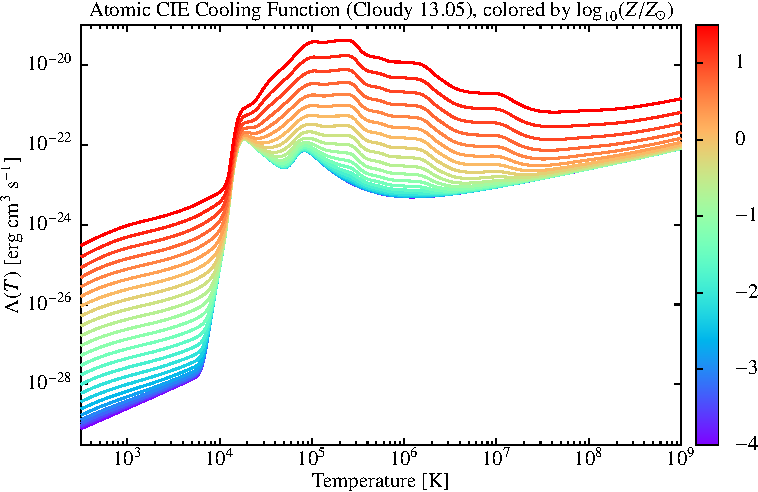
\includegraphics[width=160mm]{../plots/cooling_function_Atomic_CIE_Cloudy.pdf}
 \end{center}
 \caption{Cooling function for atomic gas in collisional ionization equilibrium computed using Cloudy 08.00.}
 \label{fig:atomicCIECloudyCoolingFunction}
\end{figure}

\subsubsection{Cooling Radius}

Additional methods for cooling radius calculations can be added using the {\normalfont \ttfamily coolingRadiusMethod} directive. The directive should contain a single argument, giving the name of a subroutine to be called to initialize the method. For example, the {\normalfont \ttfamily simple} method is described by a directive:
\begin{verbatim}
 !# <coolingRadiusMethod>
 !#  <unitName>Cooling_Radius_Simple_Initialize</unitName>
 !# </coolingRadiusMethod>
\end{verbatim}
Here, {\normalfont \ttfamily Cooling\_Radius\_Simple\_Initialize} is the name of a subroutine which will be called to initialize the method. The initialization subroutine must have the following form:
\begin{verbatim}
  subroutine Method_Initialize(coolingRadiusMethod,Cooling_Radius_Get,Cooling_Radius_Growth_Rate_Get)
    implicit none
    type(varying_string),          intent(in)    :: coolingRadiusMethod
    procedure(),          pointer, intent(inout) :: Cooling_Radius_Get,Cooling_Radius_Growth_Rate_Get
    
    if (coolingRadiusMethod == 'myMethod') then
       Cooling_Radius_Get => My_Method_Get_Procedure
       Cooling_Radius_Growth_Rate_Get => My_Method_Growth_Rate_Get_Procedure
    end if
    return
  end subroutine Method_Initialize
\end{verbatim}
where {\normalfont \ttfamily myMethod} is the name of this method as will be specified by the {\normalfont \ttfamily coolingRadiusMethod} input parameter. The procedure pointer {\normalfont \ttfamily Cooling\_Radius\_Get} must be set to point to a function which returns the cooling function as described below while {\normalfont \ttfamily Cooling\_Radius\_Growth\_Rate\_Get} should be set to point to a function which returns the rate at which the cooling radius is growing. The initialization subroutine should perform any other tasks required to initialize the module (such as reading parameters etc.).

The cooling radius function must have the form:
\begin{verbatim}
 double precision function Cooling_Radius_Get(thisNode)
    implicit none
    type(treeNode), intent(inout), pointer :: thisNode
    .
    .
    .
    return
 end function Cooling_Radius_Get
\end{verbatim}
The function must return the cooling radius (in units of Mpc) for {\normalfont \ttfamily thisNode}. The cooling radius growth rate function should have the same template but return the rate at which the cooling radius grows in units of Mpc/Gyr.

Currently defined cooling radius methods are:
\begin{description}
 \item [\hyperlink{cooling.cooling_radius.simple.F90:cooling_radii_simple:cooling_radius_simple}{{\normalfont \ttfamily simple}}] Computes the cooling radius by seeking the radius at which the time available for cooling equals the cooling time. The growth rate is determined consistently based on the slope of the density profile, the density dependence of the cooling function and the rate at which the time available for cooling is increasing. This method assumes that the cooling time is a monotonic function of radius.
 \item [\hyperlink{cooling.cooling_radius.isothermal_profile.F90:cooling_radii_isothermal:cooling_radius_isothermal}{{\normalfont \ttfamily isothermal}}] Computes the cooling radius by assuming that the hot gas density profile is an isothermal profile ($\rho(r) \propto r^{-2}$), and that the cooling rate scales as density squared, $\dot{E}\propto \rho^2$, such that the cooling time scales as inverse density, $t_{\mathrm cool} \propto \rho^{-1}$. Consequently, the cooling radius grows as the square root of the time available for cooling.
\end{description}

\subsubsection{Cooling: Freefall Radius}

Additional methods for freefall radius in cooling calculations can be added using the {\normalfont \ttfamily freefallRadiusMethod} directive. The directive should contain a single argument, giving the name of a subroutine to be called to initialize the method. For example, the {\normalfont \ttfamily simple} method is described by a directive:
\begin{verbatim}
 !# <freefallRadiusMethod>
 !#  <unitName>Freefall_Radius_Dark_Matter_Halo_Initialize</unitName>
 !# </freefallRadiusMethod>
\end{verbatim}
Here, {\normalfont \ttfamily Freefall\_Radius\_Dark\_Matter\_Halo\_Initialize} is the name of a subroutine which will be called to initialize the method. The initialization subroutine must have the following form:
\begin{verbatim}
  subroutine Method_Initialize(freefallRadiusMethod,Freefall_Radius_Get,Freefall_Radius_Growth_Rate_Get)
    implicit none
    type(varying_string),          intent(in)    :: freefallRadiusMethod
    procedure(),          pointer, intent(inout) :: Freefall_Radius_Get,Freefall_Radius_Growth_Rate_Get
    
    if (freefallRadiusMethod == 'myMethod') then
       Freefall_Radius_Get             => My_Method_Get_Procedure
       Freefall_Radius_Growth_Rate_Get => My_Method_Growth_Rate_Get_Procedure
    end if
    return
  end subroutine Method_Initialize
\end{verbatim}
where {\normalfont \ttfamily myMethod} is the name of this method as will be specified by the {\normalfont \ttfamily freefallRadiusMethod} input parameter. The procedure pointer {\normalfont \ttfamily Freefall\_Radius\_Get} must be set to point to a function which returns the freefall radius as described below while {\normalfont \ttfamily Freefall\_Radius\_Growth\_Rate\_Get} should be set to point to a function which returns the rate at which the freefall radius is growing. The initialization subroutine should perform any other tasks required to initialize the module (such as reading parameters etc.).

The freefall radius function must have the form:
\begin{verbatim}
 double precision function Freefall_Radius_Get(thisNode)
    implicit none
    type(treeNode), intent(inout), pointer :: thisNode
    .
    .
    .
    return
 end function Freefall_Radius_Get
\end{verbatim}
The function must return the freefall radius (in units of Mpc) for {\normalfont \ttfamily thisNode}. The freefall radius growth rate function should have the same template but return the rate at which the freefall radius grows in units of Mpc/Gyr.

Currently defined freefall radius methods are:
\begin{description}
 \item [\hyperlink{cooling.freefall_radii.dark_matter_halo.F90:freefall_radii_dark_matter_halo:freefall_radius_dark_matter_halo}{{\normalfont \ttfamily darkMatterHalo}}] Computes the freefall radius by finding the radius in the dark matter halo profile from which a test particle could have free-fallen to zero radius (assuming it began at rest) in the time available for freefall.
\end{description}

\subsubsection{Cooling: Infall Radius}

Additional methods for the infall radius in cooling calculations can be added using the {\normalfont \ttfamily infallRadiusMethod} directive. The directive should contain a single argument, giving the name of a subroutine to be called to initialize the method. For example, the {\normalfont \ttfamily coolingRadius} method is described by a directive:
\begin{verbatim}
 !# <infallRadiusMethod>
 !#  <unitName>Infall_Radius_Cooling_Radius_Initialize</unitName>
 !# </infallRadiusMethod>
\end{verbatim}
Here, {\normalfont \ttfamily Infall\_Radius\_Cooling\_Radius\_Initialize} is the name of a subroutine which will be called to initialize the method. The initialization subroutine must have the following form:
\begin{verbatim}
  subroutine Method_Initialize(infallRadiusMethod,Infall_Radius_Get,Infall_Radius_Growth_Rate_Get)
    implicit none
    type(varying_string),          intent(in)    :: infallRadiusMethod
    procedure(),          pointer, intent(inout) :: Infall_Radius_Get,Infall_Radius_Growth_Rate_Get
    
    if (infallRadiusMethod == 'myMethod') then
       Infall_Radius_Get             => My_Method_Get_Procedure
       Infall_Radius_Growth_Rate_Get => My_Method_Growth_Rate_Get_Procedure
    end if
    return
  end subroutine Method_Initialize
\end{verbatim}
where {\normalfont \ttfamily myMethod} is the name of this method as will be specified by the {\normalfont \ttfamily infallRadiusMethod} input parameter. The procedure pointer {\normalfont \ttfamily Infall\_Radius\_Get} must be set to point to a function which returns the infall radius as described below while {\normalfont \ttfamily Infall\_Radius\_Growth\_Rate\_Get} should be set to point to a function which returns the rate at which the infall radius is growing. The initialization subroutine should perform any other tasks required to initialize the module (such as reading parameters etc.).

The infall radius function must have the form:
\begin{verbatim}
 double precision function Infall_Radius_Get(thisNode)
    implicit none
    type(treeNode), intent(inout), pointer :: thisNode
    .
    .
    .
    return
 end function Infall_Radius_Get
\end{verbatim}
The function must return the infall radius (in units of Mpc) for {\normalfont \ttfamily thisNode}, i.e. the radius from which gas in the hot halo that is currently accreting onto the galaxy originated. The infall radius growth rate function should have the same template but return the rate at which the infall radius grows in units of Mpc/Gyr.

Currently defined infall radius methods are:
\begin{description}
 \item [\hyperlink{cooling.infall_radius.cooling_radius.F90:infall_radii_cooling_radius:infall_radius_cooling_radius}{{\normalfont \ttfamily coolingRadius}}] Assumes that the infall radius equals the cooling radius.
 \item [\hyperlink{cooling.infall_radius.cooling_and_freefall.F90:infall_radii_cooling_freefall:infall_radius_cooling_freefall}{{\normalfont \ttfamily cooling and freefall}}] Assumes that the infall radius is equal to the smaller of the cooling and freefall radii.
\end{description}

\subsubsection{Cooling Specific Angular Momentum}

Additional methods for calculations of the specific angular momentum of cooling gas can be added using the {\normalfont \ttfamily coolingSpecificAngularMomentumMethod} directive. The directive should contain a single argument, giving the name of a subroutine to be called to initialize the method. For example, the {\normalfont \ttfamily simple} method is described by a directive:
\begin{verbatim}
 !# <coolingSpecificAngularMomentumMethod>
 !#  <unitName>Cooling_Specific_AM_Constant_Rotation_Initialize</unitName>
 !# </coolingSpecificAngularMomentumMethod>
\end{verbatim}
Here, {\normalfont \ttfamily Cooling\_Time\_Simple\_Initialize} is the name of a subroutine which will be called to initialize the method. The initialization subroutine must have the following form:
\begin{verbatim}
  subroutine Method_Initialize(coolingSpecificAngularMomentumMethod,Cooling_Specific_Angular_Momentum_Get)
    implicit none
    type(varying_string),          intent(in)    :: coolingSpecificAngularMomentumMethod
    procedure(),          pointer, intent(inout) :: Cooling_Specific_Angular_Momentum_Get
    
    if (coolingSpecificAngularMomentumMethod == 'myMethod') then
       Cooling_Specific_Angular_Momentum_Get => My_Method_Get_Procedure
    end if
    return
  end subroutine Method_Initialize
\end{verbatim}
where {\normalfont \ttfamily myMethod} is the name of this method as will be specified by the {\normalfont \ttfamily coolingSpecificAngularMomentumMethod} input parameter. The procedure pointer {\normalfont \ttfamily Cooling\_Specific\_Angular\_Momentum\_Get} must be set to point to a function which returns the specific angular momentum of cooling gas. The initialization subroutine should perform any other tasks required to initialize the module (such as reading parameters etc.).

The specific angular momentum of cooling gas function must have the form:
\begin{verbatim}
 double precision function Cooling_Specific_Angular_Momentum_Get(thisNode)
    implicit none
    type(treeNode), intent(inout), pointer :: thisNode
    .
    .
    .
    return
 end function Cooling_Specific_Angular_Momentum_Get
\end{verbatim}
The function must return the specific angular momentum (in units of km/s Mpc) of gas that is cooling in {\normalfont \ttfamily thisNode}.

Currently defined specific angular momentum of cooling gas methods are:
\begin{description}
 \item [\hyperlink{cooling.specific_angular_momentum.constant_rotation.F90:cooling_specific_angular_momenta_constant_rotation:cooling_specific_angular_momentum_constant_rotation}{{\normalfont \ttfamily constantRotation}}] Computes the specific angular momentum of the cooling gas based on the cooling radius, mean specific angular momentum and the assumption of a constant mean rotation speed in the cooling gas as a function of radius.
 \item [\hyperlink{cooling.specific_angular_momentum.mean.F90:cooling_specific_angular_momenta_mean:cooling_specific_angular_momentum_mean}{{\normalfont \ttfamily mean}}] Assumes that the specific angular momentum of the cooling gas always equals the mean specific angular momentum of the hot halo.
\end{description}

\subsubsection{Cooling Time Available}

Additional methods for the time available for cooling can be added using the {\normalfont \ttfamily coolingTimeAvailableMethod} directive. The directive should contain a single argument, giving the name of a subroutine to be called to initialize the method. For example, the {\normalfont \ttfamily White-Frenk} method is described by a directive:
\begin{verbatim}
 !# <coolingTimeAvailableMethod>
 !#  <unitName>Cooling_Time_Available_WF_Initialize</unitName>
 !# </coolingTimeAvailableMethod>
\end{verbatim}
Here, {\normalfont \ttfamily Cooling\_Time\_Available\_WF\_Initialize} is the name of a subroutine which will be called to initialize the method. The initialization subroutine must have the following form:
\begin{verbatim}
  subroutine Method_Initialize(coolingTimeAvailableMethod,Cooling_Time_Available_Get&
       &,Cooling_Time_Available_Increase_Rate_Get)
    implicit none
    type(varying_string),          intent(in)    :: coolingTimeAvailableMethod
    procedure(),          pointer, intent(inout) :: Cooling_Time_Available_Get,Cooling_Time_Available_Increase_Rate_Get
    
    if (coolingTimeAvailableMethod == 'myMethod') then
      Cooling_Time_Available_Get               => My_Method_Get
      Cooling_Time_Available_Increase_Rate_Get => My_Method_Increase_Rate_Get
    end if
    return
  end subroutine Method_Initialize
\end{verbatim}
where {\normalfont \ttfamily myMethod} is the name of this method as will be specified by the {\normalfont \ttfamily coolingTimeAvailableMethod} input parameter. The procedure pointers {\normalfont \ttfamily Cooling\_Time\_Available\_Get} and {\normalfont \ttfamily Cooling\_Time\_Available\_Increase\_Rate\_Get} must be set to point to functions which return the time available for cooling and the rate of increase of this time respectively. The initialization subroutine should perform any other tasks required to initialize the module (such as reading parameters etc.).

The cooling time available functions must have the form:
\begin{verbatim}
 double precision function Cooling_Time_Available_Get(thisNode)
    implicit none
    type(treeNode),   intent(inout), pointer :: thisNode
    .
    .
    .
    return
 end function Cooling_Time_Available_Get
\end{verbatim}
The first function must return the time available for cooling (in units of Gyr) for {\normalfont \ttfamily thisNode}, while the second must return the rate of increase of this time. 

Currently defined cooling time available methods are:
\begin{description}
 \item [\hyperlink{cooling.time_available.White-Frenk.F90:cooling_time_available_white_frenk:cooling_time_available_wf}{{\normalfont \ttfamily White-Frenk}}] The time available is set to a value between the age of the Universe and the dynamical time of the halo, depending on the interpolating parameter {\normalfont \ttfamily [coolingTimeAvailableAgeFactor]};
 \item [\hyperlink{cooling.time_available.halo_formation.F90:cooling_times_available_halo_formation:cooling_time_available_halo_formation}{{\normalfont \ttfamily haloFormation}}] The time available for cooling is set equal to the current time minus the formation time of the halo.
\end{description}

\subsubsection{Cooling Time Available For Freefall}

Additional methods for the time available for freefall in cooling calculations can be added using the {\normalfont \ttfamily freefallTimeAvailableMethod} directive. The directive should contain a single argument, giving the name of a subroutine to be called to initialize the method. For example, the {\normalfont \ttfamily haloFormation} method is described by a directive:
\begin{verbatim}
 !# <freefallTimeAvailableMethod>
 !#  <unitName>Freefall_Time_Available_Halo_Formation_Initialize</unitName>
 !# </freefallTimeAvailableMethod>
\end{verbatim}
Here, {\normalfont \ttfamily Freefall\_Time\_Available\_Halo\_Formation\_Initialize} is the name of a subroutine which will be called to initialize the method. The initialization subroutine must have the following form:
\begin{verbatim}
  subroutine Method_Initialize(freefallTimeAvailableMethod,Freefall_Time_Available_Get&
       &,Freefall_Time_Available_Increase_Rate_Get)
    implicit none
    type(varying_string),          intent(in)    :: freefallTimeAvailableMethod
    procedure(),          pointer, intent(inout) :: Freefall_Time_Available_Get,Freefall_Time_Available_Increase_Rate_Get
    
    if (freefallTimeAvailableMethod == 'myMethod') then
      Freefall_Time_Available_Get               => My_Method_Get
      Freefall_Time_Available_Increase_Rate_Get => My_Method_Increase_Rate_Get
    end if
    return
  end subroutine Method_Initialize
\end{verbatim}
where {\normalfont \ttfamily myMethod} is the name of this method as will be specified by the {\normalfont \ttfamily freefallTimeAvailableMethod} input parameter. The procedure pointers {\normalfont \ttfamily Freefall\_Time\_Available\_Get} and {\normalfont \ttfamily Freefall\_Time\_Available\_Increase\_Rate\_Get} must be set to point to functions which return the time available for freefal in cooling calculations and the rate of increase of this time respectively. The initialization subroutine should perform any other tasks required to initialize the module (such as reading parameters etc.).

The freefall time available functions must have the form:
\begin{verbatim}
 double precision function Freefall_Time_Available_Get(thisNode)
    implicit none
    type(treeNode),   intent(inout), pointer :: thisNode
    .
    .
    .
    return
 end function Freefall_Time_Available_Get
\end{verbatim}
The first function must return the time available for freefall cooling calculations (in units of Gyr) for {\normalfont \ttfamily thisNode}, while the second must return the rate of increase of this time. 

Currently defined freefall time available methods are:
\begin{description}
 \item [\hyperlink{cooling.freefall_time_available.halo_formation.F90:freefall_times_available_halo_formation:freefall_time_available_halo_formation}{{\normalfont \ttfamily haloFormation}}] The time available for cooling is set equal to the current time minus the formation time of the halo.
\end{description}

\subsubsection{Cooling Time}

Additional methods for cooling time calculations can be added using the {\normalfont \ttfamily coolingTimeMethod} directive. The directive should contain a single argument, giving the name of a subroutine to be called to initialize the method. For example, the {\normalfont \ttfamily simple} method is described by a directive:
\begin{verbatim}
 !# <coolingTimeMethod>
 !#  <unitName>Cooling_Time_Simple_Initialize</unitName>
 !# </coolingTimeMethod>
\end{verbatim}
Here, {\normalfont \ttfamily Cooling\_Time\_Simple\_Initialize} is the name of a subroutine which will be called to initialize the method. The initialization subroutine must have the following form:
\begin{verbatim}
  subroutine Method_Initialize(coolingTimeMethod,Cooling_Time_Get,Cooling_Time_Density_Log_Slope_Get,Cooling_Time_Temperature_Log_Slope_Get)
    implicit none
    type(varying_string),          intent(in)    :: coolingTimeMethod
    procedure(),          pointer, intent(inout) :: Cooling_Time_Get,Cooling_Time_Density_Log_Slope_Get,Cooling_Time_Temperature_Log_Slope_Get
    
    if (coolingTimeMethod == 'myMethod') then
       Cooling_Time_Get => My_Method_Get_Procedure
       Cooling_Time_Density_Log_Slope_Get     => My_Method_Density_Log_Slope_Procedure
       Cooling_Time_Temperature_Log_Slope_Get => My_Method_Temperature_Log_Slope_Procedure
    end if
    return
  end subroutine Method_Initialize
\end{verbatim}
where {\normalfont \ttfamily myMethod} is the name of this method as will be specified by the {\normalfont \ttfamily coolingTimeMethod} input parameter. The procedure pointer {\normalfont \ttfamily Cooling\_Time\_Get} must be set to point to a function which returns the cooling function as described below while the other two pointers should point to functions which return the appropriate logarithmic slope. The initialization subroutine should perform any other tasks required to initialize the module (such as reading parameters etc.).

The cooling time function must have the form:
\begin{verbatim}
 double precision function Cooling_Time_Get(temperature,density,abundances,chemicalDensities,radiation)
    implicit none
    double precision,                  intent(in) :: temperature,density
    type(abundancesStructure),         intent(in) :: abundances
    type(chemicalAbundancesStructure), intent(in) :: chemicalDensities
    type(radiationStructure),          intent(in) :: radiation
    .
    .
    .
    return
 end function Cooling_Time_Get
\end{verbatim}
The function must return the cooling time (in units of Gyr) for at the specified {\normalfont \ttfamily temperature}, {\normalfont \ttfamily density} and for composition and radiation field as specified by the {\normalfont \ttfamily abundances}, {\normalfont \ttfamily chemicalDensities} and {\normalfont \ttfamily radiation} structures. The logarithmic slope functions should have the same template, but return the logarithmic slope of the cooling time with respect to the appropriate variable instead.

Currently defined cooling time methods are:
\begin{description}
 \item [\hyperlink{cooling.cooling_time.simple.F90:cooling_times_simple:cooling_time_simple}{{\normalfont \ttfamily simple}}] Compute the cooling time as the ratio of the gas thermal energy density to the volume rate of radiative energy loss. The gas is assumed to have an effective number of degrees of freedom specified by the {\normalfont \ttfamily coolingTimeSimpleDegreesOfFreedom} parameter.
\end{description}

\subsubsection{Cosmological Mass Root Variance}

Additional methods for computing the cosmological mass root variance, $\sigma(M)$, can be added using the {\normalfont \ttfamily cosmologicalMassVarianceMethod} directive. The directive should contain a single argument, giving the name of a subroutine to be called to initialize the method. For example, the {\normalfont \ttfamily filteredPowerSpectrum} method is described by a directive:
\begin{verbatim}
  !# <cosmologicalMassVarianceMethod>
  !#  <unitName>Cosmological_Mass_Variance_Filtered_Power_Spectrum_Initialize</unitName>
  !# </cosmologicalMassVarianceMethod>
\end{verbatim}
Here, {\normalfont \ttfamily Cosmological\_Mass\_Variance\_Filtered\_Power\_Spectrum\_Initialize} is the name of a subroutine which will be called to initialize the method. The initialization subroutine must have the following form:
\begin{verbatim}
  subroutine Method_Initialize(cosmologicalMassVarianceMethod,Cosmological_Mass_Variance_Tabulate)
    implicit none
    type     (varying_string),          intent(in   ) :: cosmologicalMassVarianceMethod
    procedure(               , pointer, intent(inout) :: Cosmological_Mass_Variance_Tabulate
    
    if (cosmologicalMassVarianceMethod == 'myMethod') then
       Cosmological_Mass_Variance_Tabulate => My_Method_Tabulate
       .
       .
       .
    end if
    return
  end subroutine Method_Initialize
\end{verbatim}
where {\normalfont \ttfamily myMethod} is the name of this method as will be specified by the {\normalfont \ttfamily cosmologicalMassVarianceMethod} input parameter. The procedure pointer {\normalfont \ttfamily Cosmological\_Mass\_Variance\_Tabulate} must be set to point to a function which populates a {\normalfont \ttfamily table1D} object with a tabulation of $\sigma(M)$. The initialization subroutine should perform any other tasks required to initialize the module (such as reading parameters etc.).

The tabulation function must have the form:
\begin{verbatim}
   subroutine Cosmological_Mass_Variance_Filtered_Power_Spectrum(mass,massNormalization,sigmaNormalization,sigmaTable)
    implicit none
    double precision         , intent(in   )              :: mass,massNormalization
    double precision         , intent(inout)              :: sigmaNormalization
    class           (table1D), intent(inout), allocatable :: sigmaTable
    .
    .
    return
   end subroutine Cosmological_Mass_Variance_Filtered_Power_Spectrum
\end{verbatim}
The function should allocate {\normalfont \ttfamily sigmaTable} to a suitable type of {\normalfont \ttfamily table1D} object and populate it with a tabulation of $\sigma(M)$ which includes the given {\normalfont \ttfamily mass}. On input, the required normalization of $\sigma(M)$ at mass {\normalfont \ttfamily massNormalization} is given by {\normalfont \ttfamily sigmaNormalization}. The function should divide this value by the unnormalized value of $\sigma(M)$---this is used to normalize the cosmological power spectrum.

Currently defined cosmological mass root variance methods are:
\begin{description}
 \item [{\normalfont \ttfamily filteredPowerSpectrum}] The mass root variance is found by integrating over the transferred linear power spectrum multiplied by the selected window function (see \S\ref{sec:PowerSpectrumWindowFunction}).
\end{description}

\subsubsection{Critical Overdensity for Halo Collapse}

Additional methods for the critical linear theory overdensity for halo collapse can be added using the {\normalfont \ttfamily criticalOverdensityMethod} directive. The directive should contain a single argument, giving the name of a subroutine to be called to initialize the method. For example, the {\normalfont \ttfamily sphericalTopHat} method is described by a directive:
\begin{verbatim}
  !# <criticalOverdensityMethod>
  !#  <unitName>Spherical_Collape_Delta_Critical_Initialize</unitName>
  !# </criticalOverdensityMethod>
\end{verbatim}
Here, {\normalfont \ttfamily Spherical\_Collape\_Delta\_Critical\_Initialize} is the name of a subroutine which will be called to initialize the method. The initialization subroutine must have the following form:
\begin{verbatim}
  subroutine Method_Initialize(criticalOverdensityMethod,Critical_Overdensity_Tabulate)
    implicit none
    type(varying_string),          intent(in)    :: criticalOverdensityMethod
    procedure(),          pointer, intent(inout) :: Critical_Overdensity_Tabulate
    
    if (criticalOverdensityMethod.eq.'myMethod') then
       Critical_Overdensity_Tabulate => My_Do_Tabulate
       .
       .
       .
    end if
    return
  end subroutine Method_Initialize
\end{verbatim}
where {\normalfont \ttfamily myMethod} is the name of this method as will be specified by the {\normalfont \ttfamily criticalOverdensityMethod} input parameter. The procedure pointer {\normalfont \ttfamily Critical\_Overdensity\_Tabulate} must be set to point to a subroutine which tabulates the critical overdensity as described below. The initialization subroutine should perform any other tasks required to initialize the module (such as reading parameters etc.).

The tabulation subroutine must have the form:
\begin{verbatim}
   subroutine Critical_Overdensity_Tabulate(time,deltaCritNumberPoints,deltaCritTime,deltaCritDeltaCrit)
    implicit none
    double precision, intent(in)                               :: time
    integer,          intent(out)                              :: deltaCritNumberPoints
    double precision, intent(inout), allocatable, dimension(:) :: deltaCritTime,deltaCritDeltaVirial
    .
    .
    .
    return
   end subroutine Critical_Overdensity_Tabulate
\end{verbatim}
The subroutine must tabulate the critical overdensity in array {\normalfont \ttfamily deltaCritDeltaVirial()} as a function of wavenumber {\normalfont \ttfamily deltaCritTime()} (these arrays must be allocated to the correct size, and may be prevously allocated, therefore requiring a deallocation). The number of tabulated points should be returned in {\normalfont \ttfamily deltaCritNumberPoints}. The subroutine should ensure that the currently requested {\normalfont \ttfamily time} is within the range of the tabulated function (preferably with some buffer).

Currently defined critical overdensity methods are:
\begin{description}
 \item [{\normalfont \ttfamily sphericalTopHat}] The critical overdensity is computed for a Universe containing collisionless matter and a cosmological constant following the spherical top hat collapse model (see, for example, \citealt{percival_cosmological_2005}).
 \item [{\normalfont \ttfamily Kitayama-Suto1996}] The critical overdensity is computed using the fitting formula of \cite{kitayama_semianalytic_1996}, and is therefore valid only for flat cosmological models.
 \item [{\normalfont \ttfamily fixed}] The critical overdensity is set to a fixed number divided by the linear growth factor.
\end{description}

\subsubsection{Critical Overdensity for Halo Collapse: Mass Scaling}

Additional methods for the mass scaling of the critical linear theory overdensity for halo collapse can be added using the {\normalfont \ttfamily criticalOverdensityMassScalingMethod} directive. The directive should contain a single argument, giving the name of a subroutine to be called to initialize the method. For example, the {\normalfont \ttfamily warm dark matter} method is described by a directive:
\begin{verbatim}
  !# <criticalOverdensityMassScalingMethod>
  !#  <unitName>Critical_Overdensity_Mass_Scaling_WDM_Initialize</unitName>
  !# </criticalOverdensityMassScalingMethod>
\end{verbatim}
Here, {\normalfont \ttfamily Critical\_Overdensity\_Mass\_Scaling\_WDM\_Initialize} is the name of a subroutine which will be called to initialize the method. The initialization subroutine must have the following form:
\begin{verbatim}
  subroutine Method_Initialize(criticalOverdensityMassScalingMethod, &
   & Critical_Overdensity_Mass_Scaling_Get,Critical_Overdensity_Mass_Scaling_Gradient_Get)
    implicit none
    type(varying_string),          intent(in)    :: criticalOverdensityMassScalingMethod
    procedure(),          pointer, intent(inout) :: Critical_Overdensity_Mass_Scaling_Get, &
   &                                                Critical_Overdensity_Mass_Scaling_Gradient_Get
    
    if (criticalOverdensityMassScalingMethod == 'myMethod') then
       Critical_Overdensity_Mass_Scaling_Get          => My_Do_Tabulate
       Critical_Overdensity_Mass_Scaling_Gradient_Get => My_Do_Gradient_Tabulate
       .
       .
       .
    end if
    return
  end subroutine Method_Initialize
\end{verbatim}
where {\normalfont \ttfamily myMethod} is the name of this method as will be specified by the {\normalfont \ttfamily criticalOverdensityMassScalingMethod} input parameter. The procedure pointers {\normalfont \ttfamily Critical\_Overdensity\_Mass\_Scaling\_Get} and {\normalfont \ttfamily Critical\_Overdensity\_Mass\_Scaling\_Gradient\_Get} must be set to point to functions which return the critical overdensity mass scaling and its gradient as described below. The initialization subroutine should perform any other tasks required to initialize the module (such as reading parameters etc.).

The mass scaling function must have the form:
\begin{verbatim}
   double precision function Critical_Overdensity_Mass_Scaling_Get(mass)
    implicit none
    double precision, intent(in) :: mass
    .
    .
    .
    return
   end function Critical_Overdensity_Mass_Scaling_Get
\end{verbatim}
The function should return the factor by which the critical overdensity for collapse at the given {\normalfont \ttfamily mass} scale (given in units of $M_{\odot}$) differs from that for the case $M\rightarrow\infty$. The mass scaling gradient function should have the same form, but should return the derivative of the scaling with respect to mass.

Currently defined critical overdensity mass scaling methods are:
\begin{description}
 \item [{\normalfont \ttfamily null}] The critical overdensity is assumed to have no scaling with mass;
 \item [{\normalfont \ttfamily warm dark matter}] The mass scaling is computed for warm dark matter using a fitting function to the results of \cite{barkana_constraints_2001}.
\end{description}

\subsubsection{Dark Matter Halo Spin Distribution}\label{sec:HaloSpinDistribution}\index{dark matter halo!spin!distribution}\index{spin!dark matter halo}

Additional methods for the dark matter density profile concentration can be added using the {\normalfont \ttfamily haloSpinDistributionMethod} directive. The directive should contain a single argument, giving the name of a subroutine to be called to initialize the method. For example, the {\normalfont \ttfamily Gao2008} method is described by a directive:
\begin{verbatim}
 !# <haloSpinDistributionMethod>
 !#  <unitName>Halo_Spin_Distribution_Bett2007_Initialize</unitName>
 !# </haloSpinDistributionMethod>
\end{verbatim}
Here, {\normalfont \ttfamily Halo\_Spin\_Distribution\_Bett2007\_Initialize} is the name of a subroutine which will be called to initialize the method. The initialization subroutine must have the following form:
\begin{verbatim}
  subroutine Method_Initialize(haloSpinDistributionMethod,Halo_Spin_Sample_Get)
    implicit none
    type(varying_string),          intent(in)    :: haloSpinDistributionMethod
    procedure(),          pointer, intent(inout) :: Halo_Spin_Sample_Get
    
    if (haloSpinDistributionMethod == 'myMethod') then
       Halo_Spin_Sample_Get => My_Spin_Sample_Get
       .
       .
       .
    end if
    return
  end subroutine Method_Initialize
\end{verbatim}
where {\normalfont \ttfamily myMethod} is the name of this method as will be specified by the {\normalfont \ttfamily haloSpinDistributionMethod} input parameter. The procedure pointer {\normalfont \ttfamily Halo\_Spin\_Sample\_Get} must be set to point to a function which returns a spin parameter drawn at random from a distribution. The initialization subroutine should perform any other tasks required to initialize the module (such as reading parameters etc.).

The spin parameter function must have the form:
\begin{verbatim}
  double precision function My_Spin_Distribution_Sample(thisNode)
    implicit none
    type(treeNode), intent(inout), pointer :: thisNode
    .
    .
    .
    return
  end function My_Spin_Distribution_Sample
\end{verbatim}
The function should compute and return a spin parameter for {\normalfont \ttfamily thisNode} drawn at random from a distribution.

Currently defined spin distribution methods are:
\begin{description}
 \item [{\normalfont \ttfamily lognormal}] The spin is drawn from a lognormal distribution with median {\normalfont \ttfamily [lognormalSpinDistributionMedian]} and width {\normalfont \ttfamily [lognormalSpinDistributionSigma]}.
 \item [{\normalfont \ttfamily Bett2007}] The spin is drawn from the distribution found by \cite{bett_spin_2007}. The $\lambda_0$ and $\alpha$ parameter of Bett et al.'s distribution are set by the {\normalfont \ttfamily [spinDistributionBett2007Lambda0]} and {\normalfont \ttfamily [spinDistributionBett2007Alpha]} input parameters.
 \item [{\normalfont \ttfamily deltaFunction}] The spin is drawn from a delta function distribution, i.e. a value equal to {\normalfont \ttfamily [deltaFunctionSpinDistributionSpin]} is always returned.
\end{description}

\subsubsection{Dark Matter Halo Mass Loss Rates}\label{sec:HaloMassLossRates}\index{dark matter halo!mass loss}\index{mass loss!dark matter halo}

Additional methods for dark matter halo mass loss rates can be added using the {\normalfont \ttfamily darkMatterHaloMassLossRateMethod} directive. The directive should contain a single argument, giving the name of a subroutine to be called to initialize the method. For example, the {\normalfont \ttfamily van den Bosch 2005} method is described by a directive:
\begin{verbatim}
 !# <darkMatterHaloMassLossRateMethod>
 !#  <unitName>Dark_Matter_Halos_Mass_Loss_Rate_vanDenBosch_Initialize</unitName>
 !# </darkMatterHaloMassLossRateMethod>
\end{verbatim}
Here, {\normalfont \ttfamily Dark\_Matter\_Halos\_Mass\_Loss\_Rate\_vanDenBosch\_Initialize} is the name of a subroutine which will be called to initialize the method. The initialization subroutine must have the following form:
\begin{verbatim}
  subroutine Method_Initialize(darkMatterHaloMassLossRateMethod,Dark_Matter_Halos_Mass_Loss_Rate_Get)
    implicit none
    type(varying_string),          intent(in)    :: darkMatterHaloMassLossRateMethod
    procedure(),          pointer, intent(inout) :: Dark_Matter_Halos_Mass_Loss_Rate_Get
    
    if (darkMatterHaloMassLossRateMethod == 'myMethod') then
       Dark_Matter_Halos_Mass_Loss_Rate_Get => My_Mass_Loss_Rate_Get
       .
       .
       .
    end if
    return
  end subroutine Method_Initialize
\end{verbatim}
where {\normalfont \ttfamily myMethod} is the name of this method as will be specified by the {\normalfont \ttfamily darkMatterHaloMassLossRateMethod} input parameter. The procedure pointer {\normalfont \ttfamily Dark\_Matter\_Halos\_Mass\_Loss\_Rate\_Get} must be set to point to a function which returns a spin parameter drawn at random from a distribution. The initialization subroutine should perform any other tasks required to initialize the module (such as reading parameters etc.).

The mass loss rate function must have the form:
\begin{verbatim}
  double precision function My_Mass_Loss_Rate(thisNode)
    implicit none
    type(treeNode), intent(inout), pointer :: thisNode
    .
    .
    .
    return
  end function My_Mass_Loss_Rate
\end{verbatim}
The function should compute and return the mass loss rate from {\normalfont \ttfamily thisNode} in units of $M_\odot/$Gyr.

Currently defined halo mass loss rate methods are:
\begin{description}
 \item [{\normalfont \ttfamily null}] Always returns zero mass loss rate.
 \item [{\normalfont \ttfamily vanDenBosch2005}] Uses the algorithm of \cite{van_den_bosch_mass_2005} to compute the mass loss rate.
\end{description}

\subsubsection{Excursion Set Barrier}\label{sec:excursionSetBarrierMethod}

Additional methods for the excursion set barrier can be added using the {\normalfont \ttfamily excursionSetBarrierMethod} directive. The directive should contain a single argument, giving the name of a subroutine to be called to initialize the method. For example, the {\normalfont \ttfamily linear} method is described by a directive:
\begin{verbatim}
 !# <excursionSetBarrierMethod>
 !#  <unitName>Excursion_Sets_Barriers_Linear_Initialize</unitName>
 !# </excursionSetBarrierMethod>
\end{verbatim}
Here, {\normalfont \ttfamily Excursion\_Sets\_Barriers\_Linear\_Initialize} is the name of a subroutine which will be called to initialize the method. The initialization subroutine must have the following form:
\begin{verbatim}
  subroutine Method_Initialize(excursionSetBarrierMethodExcursion_Sets_Barrier_Get,Excursion
_Sets_Barrier_Gradient_Get,barrierName)
    implicit none
    type     (varying_string  ),         intent(in   ) :: excursionSetBarrierMethod
    procedure(double precision),pointer, intent(inout) :: Excursion_Sets_Barrier_Get,Excursion_Sets_Barrier_Gradient
_Get
    type(varying_string),                intent(inout) :: barrierName

    if (excursionSetBarrierMethod == 'myMethod') then
      Excursion_Sets_Barrier_Get          => My_Barrier
      Excursion_Sets_Barrier_Gradient_Get => My_Barrier_Gradient
      barrierName=barrierName//":myLabel"
    end if
    return
  end subroutine Method_Initialize
\end{verbatim}
where {\normalfont \ttfamily myMethod} is the name of this method as will be specified by the {\normalfont \ttfamily excursionSetBarrierMethod} input parameter. The procedure pointers {\normalfont \ttfamily Excursion\_Sets\_Barrier\_Get}, and {\normalfont \ttfamily Excursion\_Sets\_Barrier\_Gradient\_Get} must be set to point functions which return the barrier and its gradient respectively, as described below. The initialization subroutine should also append a descriptive label to the {\normalfont \ttfamily barrierName} argument. The initialization subroutine should perform any other tasks required to initialize the module (such as reading parameters etc.).

The barrier and barrier gradient functions must have the form:
\begin{verbatim}
 double precision function Excursion_Sets_Barrier(variance,time)
    implicit none
    double precision, intent(in) :: variance,time
    .
    .
    .
    return
 end function Excursion_Sets_Barrier
\end{verbatim}
The barrier function must return the barrier at the specified {\normalfont \ttfamily variance} and {\normalfont \ttfamily time}, while the barrier gradient function should return the derivative with respect to variance of the same barrier.

Currently defined excursion set barrier methods are:
\begin{description}
 \item [{\normalfont \ttfamily linear}] A linear ($1^{\mathrm st}$-order polynomial) barrier;
  \item [{\normalfont \ttfamily quadratic}] A quadratic ($2^{\mathrm nd}$-order polynomial);
  \item [{\normalfont \ttfamily criticalOverdensity}] A barrier equal to the critical overdensity for halo collapse.
\end{description}

\subsubsection{Excursion Set Barrier First Crossing Distribution}\label{sec:excursionSetFirstCrossingMethod}

Additional methods for the excursion set barrier first crossing distribution can be added using the {\normalfont \ttfamily excursionSetFirstCrossingMethod} directive. The directive should contain a single argument, giving the name of a subroutine to be called to initialize the method. For example, the {\normalfont \ttfamily linearBarrier} method is described by a directive:
\begin{verbatim}
 !# <excursionSetFirstCrossingMethod>
 !#  <unitName>Excursion_Sets_First_Crossing_Linear_Barrier_Initialize</unitName>
 !# </excursionSetFirstCrossingMethod>
\end{verbatim}
Here, {\normalfont \ttfamily Excursion\_Sets\_First\_Crossing\_Linear\_Barrier\_Initialize} is the name of a subroutine which will be called to initialize the method. The initialization subroutine must have the following form:
\begin{verbatim}
  subroutine Method_Initialize(excursionSetFirstCrossingMethod,Excursion_Sets_First_Crossing_Probability_Get&
         &,Excursion_Sets_First_Crossing_Rate_Get,Excursion_Sets_Non_Crossing_Rate_Get)
    implicit none
    type     (varying_string  ),         intent(in   ) :: excursionSetFirstCrossingMethod
    procedure(double precision),pointer, intent(inout) :: Excursion_Sets_First_Crossing_Probability_Get&
         &,Excursion_Sets_First_Crossing_Rate_Get,Excursion_Sets_Non_Crossing_Rate_Get
    
    if (excursionSetFirstCrossingMethod == 'myMethod') then
       Excursion_Sets_First_Crossing_Probability_Get => My_First_Crossing_Probability
       Excursion_Sets_First_Crossing_Rate_Get        => My_First_Crossing_Rate
       Excursion_Sets_Non_Crossing_Rate_Get          => My_Non_Crossing_Rate
    end if
    return
  end subroutine Method_Initialize
\end{verbatim}
where {\normalfont \ttfamily myMethod} is the name of this method as will be specified by the {\normalfont \ttfamily excursionSetFirstCrossingMethod} input parameter. The procedure pointers {\normalfont \ttfamily Excursion\_Sets\_First\_Crossing\_Probability\_Get}, {\normalfont \ttfamily Excursion\_Sets\_First\_Crossing\_Rate\_Get}, and {\normalfont \ttfamily Excursion\_Sets\_Non\_Crossing\_Rate\_Get} must be set to point functions which return the first crossing probability, first crossing probability rate and noncrossing rate as described below. The initialization subroutine should perform any other tasks required to initialize the module (such as reading parameters etc.).

The first crossing probability function must have the form:
\begin{verbatim}
 double precision function Excursion_Sets_First_Crossing_Probability(variance,time)
    implicit none
    double precision, intent(in) :: variance,time
    .
    .
    .
    return
 end function Excursion_Sets_First_Crossing_Probability
\end{verbatim}
The function must return the first crossing probability per unit variance at the specified {\normalfont \ttfamily variance} and {\normalfont \ttfamily time}.

The first crossing probability rate function must have the form:
\begin{verbatim}
 double precision function Excursion_Sets_First_Crossing_Rate(variance,varianceProgenitor,time)
    implicit none
    double precision, intent(in) :: variance,varianceProgenitor,time
    .
    .
    .
    return
 end function Excursion_Sets_First_Crossing_Rate
\end{verbatim}
The function must return the rate of first crossing per unit variance at the specified {\normalfont \ttfamily variance} and {\normalfont \ttfamily time} for a progenitor of the specified {\normalfont \ttfamily varianceProgenitor}.

The non-crossing probability rate function must have the form:
\begin{verbatim}
 double precision function Excursion_Sets_First_Non_Crossing_Rate(variance,time)
    implicit none
    double precision, intent(in) :: variance,time
    .
    .
    .
    return
 end function Excursion_Sets_First_Non_Crossing_Rate
\end{verbatim}
The function must return the rate of trajectories which never cross the barrier at the specified {\normalfont \ttfamily variance} and {\normalfont \ttfamily time}..

Currently defined excursion set barrier first crossing methods are:
\begin{description}
 \item [{\normalfont \ttfamily linearBarrier}] Assumes the solution for a linear barrier;
 \item [{\normalfont \ttfamily Farahi}] Solves the first crossing problem using the methodology of \cite{benson_dark_2012};
 \item [{\normalfont \ttfamily ZhangHui2006}] Solves the first crossing problem using the methodology of \cite{zhang_random_2006};
 \item [{\normalfont \ttfamily ZhangHui2006HighOrder}] Solves the first crossing problem using a higher order extension of the methodology of \cite{zhang_random_2006}.
\end{description}

\subsubsection{Excursion Set Barrier Remapping}\label{sec:excursionSetBarrierRemapInitialize}

Additional methods for the excursion set barrier can be added using the {\normalfont \ttfamily excursionSetBarrierRemapInitialize} directive. The directive should contain a single argument, giving the name of a subroutine to be called to initialize the method. For example, the {\normalfont \ttfamily scale} method is described by a directive:
\begin{verbatim}
 !# <excursionSetBarrierRemapInitialize>
 !#  <unitName>Excursion_Sets_Barriers_Remap_Scale_Initialize</unitName>
 !# </excursionSetBarrierRemapInitialize>
\end{verbatim}
Here, {\normalfont \ttfamily Excursion\_Sets\_Barriers\_Remap\_Scale\_Initialize} is the name of a subroutine which will be called to initialize the method. The initialization subroutine must have the following form:
\begin{verbatim}
  subroutine Method_Initialize(excursionSetBarrierRemapMethods,barrierName, &
  & ratesCalculation,matchedCount)
    implicit none
    type(varying_string), intent(in   ), dimension(:) :: excursionSetBarrierRemapMethods
    type(varying_string), intent(inout)               :: barrierName
    logical             , intent(in   )               :: ratesCalculation
    integer             , intent(inout)               :: matchedCount

    if (any(excursionSetBarrierRemapMethods == 'myMethod')) then
       position=-1
       do i=1,size(excursionSetBarrierRemapMethods)
          if (excursionSetBarrierRemapMethods(i) == 'myMethod') then
             position=i
             exit
          end if
       end do
       if (ratesCalculation) then
          methodRatesPosition=position
       else
          methodPosition     =position
       end if
       matchedCount=matchedCount+1
       barrierName=barrierName//":myLabel"
    end if
    return
  end subroutine Method_Initialize
\end{verbatim}
where {\normalfont \ttfamily myMethod} is the name of this method as will be specified by the {\normalfont \ttfamily excursionSetBarrierRemapMethods} input parameter. The initialization subroutine should identify the position of the matched method in the {\normalfont \ttfamily excursionSetBarrierRemapMethods()} array and record that it is active for standard barrier calculations ({\normalfont \ttfamily ratesCalculation}$=${\normalfont \ttfamily false}) or for barriers used in crossing rate calculations ({\normalfont \ttfamily ratesCalculation}$=${\normalfont \ttfamily true}). It should also increment the {\normalfont \ttfamily matchedCount} argument (to allow checking that all specified barriers were matched) and append a descriptive label to the{\normalfont \ttfamily barrierName} argument. The initialization subroutine should perform any other tasks required to initialize the module (such as reading parameters etc.).

The method must provide a subroutine to compute remapping of the barrier as follows:
\begin{verbatim}
  !# <excursionSetBarrierRemap>
  !#  <unitName>Method_Barrier_Remap</unitName>
  !# </excursionSetBarrierRemap>
  subroutine Method_Barrier_Remap(barrier,variance,time,ratesCalculation,iRemap)
    implicit none
    double precision, intent(inout) :: barrier
    double precision, intent(in   ) :: variance,time
    logical         , intent(in   ) :: ratesCalculation
    integer         , intent(in   ) :: iRemap

    if ((ratesCalculation.and.iRemap == methodRatesPosition).or.(.not.ratesCalculation.and.iRemap == methodPosition)) then
     ! Do remapping.
     .
     .
     .
    end if
    return
  end subroutine Method_Barrier_Remap
\end{verbatim}
and a subroutine to compute remapping of the barrier gradient as follows:
\begin{verbatim}
  !# <excursionSetBarrierRemapGradient>
  !#  <unitName>Method_Barrier_Gradient_Remap</unitName>
  !# </excursionSetBarrierRemapGradient>
  subroutine Method_Barrier_Gradient_Remap(barrier,barrierGradient,variance,time,ratesCalculation,iRemap)
    implicit none
    double precision, intent(inout) :: barrier,barrierGradient
    double precision, intent(in   ) :: variance,time
    logical         , intent(in   ) :: ratesCalculation
    integer         , intent(in   ) :: iRemap

    if ((ratesCalculation.and.iRemap == methodRatesPosition).or.(.not.ratesCalculation.and.iRemap == methodPosition)) then
     ! Do remapping.
     .
     .
     .
    end if
    return
  end subroutine Method_Barrier_Gradient_Remap
\end{verbatim}

Currently defined excursion set barrier remapping methods are:
\begin{description}
 \item [{\normalfont \ttfamily null}] A null method which leaves the barrier unchanged;
 \item [{\normalfont \ttfamily scale}] Scales the barrier by a multiplicative factor;
 \item [{\normalfont \ttfamily Sheth-Mo-Tormen}] Remaps the barrier according to the algorithm of \cite{sheth_ellipsoidal_2001}.
\end{description}

\subsubsection{Galactic Component Radii Solver}\label{sec:galactic_radii_solvers}

Additional methods for solving for radii of galactic components can be added using the {\normalfont \ttfamily galacticStructureRadiusSolverMethod} directive. The directive should contain a single argument, giving the name of a subroutine to be called to initialize the method. For example, the {\normalfont \ttfamily simple} method is described by a directive:
\begin{verbatim}
 !# <galacticStructureRadiusSolverMethod>
 !#  <unitName>Galactic_Structure_Radii_Simple_Initialize</unitName>
 !# </galacticStructureRadiusSolverMethod>
\end{verbatim}
Here, {\normalfont \ttfamily Galactic\_Structure\_Radii\_Simple\_Initialize} is the name of a subroutine which will be called to initialize the method. The initialization subroutine must have the following form:
\begin{verbatim}
  subroutine Method_Initialize(galacticStructureRadiusSolverMethod,Galactic_Structure_Radii_Solve_Do)
    implicit none
    type(varying_string),          intent(in)    :: galacticStructureRadiusSolverMethod
    procedure(),          pointer, intent(inout) :: Galactic_Structure_Radii_Solve_Do
    
    if (galacticStructureRadiusSolverMethod == 'myMethod') Galactic_Structure_Radii_Solve_Do => My_Method_Do_Procedure
    return
  end subroutine Method_Initialize
\end{verbatim}
where {\normalfont \ttfamily myMethod} is the name of this method as will be specified by the {\normalfont \ttfamily galacticStructureRadiusSolverMethod} input parameter. The procedure pointer {\normalfont \ttfamily Galactic\_Structure\_Radii\_Solve\_Do} must be set to point to a subroutine which solves for the radii of components in a node as described below. The initialization subroutine should perform any other tasks required to initialize the module (such as reading parameters etc.).

The radii solving subroutine must have the form:
\begin{verbatim}
 subroutine Radii_Solver_Do(thisNode)
    implicit none
    type(treeNode), intent(in), pointer :: thisNode
    .
    .
    .
    return
 end subroutine Radii_Solver_Do
\end{verbatim}
The function must set the radii (and corresponding circular velocities) of all components that have a radius property in {\normalfont \ttfamily thisNode}.

Currently defined radius solver methods are:
\begin{description}
 \item [\hyperlink{galactic_structure.radius_solver.simple.F90:galactic_structure_radii_simple:galactic_structure_radii_solve_simple}{{\normalfont \ttfamily simple}}] This solver computes radii assuming that the gravitational potential is dominated by dark matter (i.e. no baryonic self-gravity is included) and that dark matter does not respond to the presence of baryons (i.e. no adiabatic contraction). It uses the ``radius solver'' (see \S\ref{sec:radius_solver}) task to interact with the node.
 \item [\hyperlink{galactic_structure.radius_solver.adiabatic.F90:galactic_structure_radii_adiabatic:galactic_structure_radii_solve_adiabatic}{{\normalfont \ttfamily adiabatic}}] This solver computes radii including the effects of self-gravity of the baryonic component and adiabatic contraction of the dark matter halo using the method of \cite{gnedin_response_2004}. It uses the ``radius solver'' (see \S\ref{sec:radius_solver}) task to interact with the node.
 \item [\hyperlink{galactic_structure.radius_solver.linear.F90:galactic_structure_radii_linear:galactic_structure_radii_solve_linear}{{\normalfont \ttfamily linear}}] This solver assumes that radii scale linearly with specific angular momentum, equalling the virial radius when the specific angular momentum equals the product of virial radii and velocities. It uses the ``radius solver'' (see \S\ref{sec:radius_solver}) task to interact with the node.
 \item [\hyperlink{galactic_structure.radius_solver.fixed.F90:galactic_structure_radii_fixed:galactic_structure_radii_solve_fixed}{{\normalfont \ttfamily fixed}}] This solver assumes that radii equal the product of virial radius of the halo and its spin parameter (with an adjustable coefficient). It uses the ``radius solver'' (see \S\ref{sec:radius_solver}) task to interact with the node.
\end{description}

\subsubsection{Galactic Component Radius Solver Initial Radius}

Additional methods for computing the initial radius in the dark matter profile when solving for adiabatic contraction of the halo can be added using the {\normalfont \ttfamily galacticStructureRadiusSolverInitialRadiusMethod} directive. The directive should contain a single argument, giving the name of a subroutine to be called to initialize the method. For example, the {\normalfont \ttfamily adiabatic} method is described by a directive:
\begin{verbatim}
 !# <galacticStructureRadiusSolverInitialRadiusMethod>
 !#  <unitName>Galactic_Structure_Initial_Radii_Adiabatic_Initialize</unitName>
 !# </galacticStructureRadiusSolverInitialRadiusMethod>
\end{verbatim}
Here, {\normalfont \ttfamily Galactic\_Structure\_Initial\_Radii\_Adiabatic\_Initialize} is the name of a subroutine which will be called to initialize the method. The initialization subroutine must have the following form:
\begin{verbatim}
  subroutine Method_Initialize(galacticStructureRadiusSolverInitialRadiusMethod,Galactic_Structure_Radius_Initial_Get,Galactic_Structure_Radius_Initial_Derivative_Get)
    implicit none
    type(varying_string),          intent(in)    :: galacticStructureRadiusSolverInitialRadiusMethod
    procedure(),          pointer, intent(inout) :: Galactic_Structure_Radius_Initial_Get,Galactic_Structure_Radius_Initial_Derivative_Get
    
    if (galacticStructureRadiusSolverInitialRadiusMethod == 'myMethod') then
       Galactic_Structure_Radius_Initial_Get            => My_Method_Get
       Galactic_Structure_Radius_Initial_Derivative_Get => My_Method_Derivative_Get
    end if
    return
  end subroutine Method_Initialize
\end{verbatim}
where {\normalfont \ttfamily myMethod} is the name of this method as will be specified by the {\normalfont \ttfamily galacticStructureRadiusSolverInitialRadiusMethod} input parameter. The procedure pointers {\normalfont \ttfamily Galactic\_Structure\_Radius\_Initial\_Get} and {\normalfont \ttfamily Galactic\_Structure\_Radius\_Initial\_Derivative\_Get} must be set to point to functions which compute the initial radius in the dark matter halo given the final radius, and the deriative of this quantity with respect to the final radius as described below. The initialization subroutine should perform any other tasks required to initialize the module (such as reading parameters etc.).

The initial radius function must have the form:
\begin{verbatim}
 double precision function Radius_Initial_Get(thisNode,radius)
    implicit none
    type            (treeNode), intent(in   ), pointer :: thisNode
    double precision          , intent(in   )          :: radius
    .
    .
    .
    return
 end function Radius_Initial_Get
\end{verbatim}
The function must return the initial radius in the dark matter halo of {\normalfont \ttfamily thisNode} corresponding to the final {\normalfont \ttfamily radius} after accounting for the effects of adiabatic contraction.

The initial radius derivative function must have the form:
\begin{verbatim}
 double precision function Radius_Initial_Derivative_Get(thisNode,radius)
    implicit none
    type            (treeNode), intent(in   ), pointer :: thisNode
    double precision          , intent(in   )          :: radius
    .
    .
    .
    return
 end function Radius_Initial_Derivative_Get
\end{verbatim}
The function must return the derivative with respect to the final {\normalfont \ttfamily radius} of initial radius in the dark matter halo of {\normalfont \ttfamily thisNode} corresponding to the final {\normalfont \ttfamily radius} after accounting for the effects of adiabatic contraction.

Currently defined initial radius methods are:
\begin{description}
 \item [\hyperlink{galactic_structure.radius_solver.initial_radii.static.F90:galactic_structure_initial_radii_static:galactic_structure_radius_initial_static}{{\normalfont \ttfamily static}}] This method assumes a static dark matter halo, and so the initial radius always equals the final radius.
 \item [\hyperlink{galactic_structure.radius_solver.initial_radii.adiabatic.F90:galactic_structure_initial_radii_adiabatic:galactic_structure_radius_initial_adiabatic}{{\normalfont \ttfamily adiabatic}}] This method assumes adiabatic contraction follows the model of \cite{gnedin_response_2004}.
\end{description}


\subsubsection{Hot Halo Ram Pressure Force}

Additional methods for the ram pressure stripping force due to hot halos can be added using the {\normalfont \ttfamily hotHaloRamPressureForceMethod} directive. The directive should contain a single argument, giving the name of a subroutine to be called to initialize the method. For example, the {\normalfont \ttfamily Font2008} method is described by a directive:
\begin{verbatim}
 !# <hotHaloRamPressureForceMethod>
 !#  <unitName>Hot_Halo_Ram_Pressure_Force_Font2008_Initialize</unitName>
 !# </hotHaloRamPressureForceMethod>
\end{verbatim}
Here, {\normalfont \ttfamily Hot\_Halo\_Ram\_Pressure\_Force\_Font2008\_Initialize} is the name of a subroutine which will be called to initialize the method. The initialization subroutine must have the following form:
\begin{verbatim}
  subroutine Method_Initialize(hotHaloRamPressureForceMethod,Hot_Halo_Ram_Pressure_Force_Get)
    implicit none
    type(varying_string),          intent(in)    :: hotHaloRamPressureForceMethod
    procedure(),          pointer, intent(inout) :: Hot_Halo_Ram_Pressure_Force_Get
    
    if (hotHaloRamPressureForceMethod == 'myMethod') Hot_Halo_Ram_Pressure_Force_Get => My_Hot_Halo_Ram_Pressure_Force_Get
    return
  end subroutine Method_Initialize
\end{verbatim}
where {\normalfont \ttfamily myMethod} is the name of this method as will be specified by the {\normalfont \ttfamily hotHaloRamPressureForceMethod} input parameter. The procedure pointer {\normalfont \ttfamily Hot\_Halo\_Ram\_Pressure\_Force\_Get} must be set to point to a function which returns ram pressure force due to the hot halo. The initialization subroutine should perform any other tasks required to initialize the module (such as reading parameters etc.).

The ram pressure force function must have the form:
\begin{verbatim}
 double precision function Hot_Halo_Ram_Pressure_Force_Get(thisNode)
    implicit none
    type(treeNode), intent(inout), pointer :: thisNode
    .
    .
    .
    return
 end function Hot_Halo_Ram_Pressure_Force_Get
\end{verbatim}
The function must return the ram pressure force acting on {\normalfont \ttfamily thisNode} due to the hot halo of its host node (in units of $M_\odot \hbox{km}^2 \hbox{s}^{-1} \hbox{Mpc}^{-3}$.

Currently defined hot halo ram pressure force methods are:
\begin{description}
 \item [\hyperlink{hot_halo.ram_pressure_force.null.F90:hot_halo_ram_pressure_force_null:hot_halo_ram_pressure_force_null_get}{{\normalfont \ttfamily null}}] Returns a zero ram pressure force.
 \item [\hyperlink{hot_halo.ram_pressure_force.Font2008.F90:hot_halo_ram_pressure_force_font2008:hot_halo_ram_pressure_force_font2008_get}{{\normalfont \ttfamily Font2008}}] Computes the ram pressure stripping radius using the algorithm of \cite{font_colours_2008}.
\end{description}

\subsubsection{Hot Halo Ram Pressure Stripping Radius}

Additional methods for the ram pressure stripping radius in hot halos can be added using the {\normalfont \ttfamily hotHaloRamPressureStrippingMethod} directive. The directive should contain a single argument, giving the name of a subroutine to be called to initialize the method. For example, the {\normalfont \ttfamily virialRadius} method is described by a directive:
\begin{verbatim}
 !# <hotHaloRamPressureStrippingMethod>
 !#  <unitName>Hot_Halo_Ram_Pressure_Stripping_Virial_Radii_Initialize</unitName>
 !# </hotHaloRamPressureStrippingMethod>
\end{verbatim}
Here, {\normalfont \ttfamily Hot\_Halo\_Ram\_Pressure\_Stripping\_Virial\_Radii\_Initialize} is the name of a subroutine which will be called to initialize the method. The initialization subroutine must have the following form:
\begin{verbatim}
  subroutine Method_Initialize(hotHaloRamPressureStrippingMethod,Hot_Halo_Ram_Pressure_Stripping_Get)
    implicit none
    type(varying_string),          intent(in)    :: hotHaloRamPressureStrippingMethod
    procedure(),          pointer, intent(inout) :: Hot_Halo_Ram_Pressure_Stripping_Get
    
    if (hotHaloRamPressureStrippingMethod == 'myMethod') Hot_Halo_Ram_Pressure_Stripping_Get => My_Hot_Halo_Ram_Pressure_Stripping_Get
    return
  end subroutine Method_Initialize
\end{verbatim}
where {\normalfont \ttfamily myMethod} is the name of this method as will be specified by the {\normalfont \ttfamily hotHaloRamPressureStrippingMethod} input parameter. The procedure pointer {\normalfont \ttfamily Hot\_Halo\_Ram\_Pressure\_Stripping\_Get} must be set to point to a function which returns the radius to which the hot halo is stripped by ram pressure forces. The initialization subroutine should perform any other tasks required to initialize the module (such as reading parameters etc.).

The ram pressure stripping radius function must have the form:
\begin{verbatim}
 double precision function Hot_Halo_Ram_Pressure_Stripping_Get(thisNode)
    implicit none
    type(treeNode), intent(inout), pointer :: thisNode
    .
    .
    .
    return
 end function Hot_Halo_Ram_Pressure_Stripping_Get
\end{verbatim}
The function must return the radius (in units of Mpc) to which the hot halo of {\normalfont \ttfamily thisNode} is stripped by ram pressure forces.

Currently defined hot halo ram pressure stripping radii methods are:
\begin{description}
 \item [\hyperlink{hot_halo.ram_pressure_stripping.virial_radius.F90:hot_halo_ram_pressure_stripping_virial_radii:hot_halo_ram_pressure_stripping_virial_radius}{{\normalfont \ttfamily virialRadius}}] Sets the ram pressure stripping radius equal to the virial radius always---effectively resulting in no ram pressure stripping.
 \item [\hyperlink{hot_halo.ram_pressure_stripping.Font2008.F90:hot_halo_ram_pressure_stripping_font2008:hot_halo_ram_pressure_stripping_font2008_get}{{\normalfont \ttfamily Font2008}}] Computes the ram pressure stripping radius using the algorithm of \cite{font_colours_2008}.
\end{description}

\subsubsection{Hot Halo Ram Pressure Stripping Timescale}

Additional methods for the ram pressure stripping timescale in hot halos can be added using the {\normalfont \ttfamily hotHaloRamPressureStrippingTimescaleMethod} directive. The directive should contain a single argument, giving the name of a subroutine to be called to initialize the method. For example, the {\normalfont \ttfamily virialRadius} method is described by a directive:
\begin{verbatim}
 !# <hotHaloRamPressureStrippingTimescaleMethod>
 !#  <unitName>Hot_Halo_Ram_Pressure_Timescales_Halo_DynTime_Initialize</unitName>
 !# </hotHaloRamPressureStrippingTimescaleMethod>
\end{verbatim}
Here, {\normalfont \ttfamily Hot\_Halo\_Ram\_Pressure\_Timescales\_Halo\_DynTime\_Initialize} is the name of a subroutine which will be called to initialize the method. The initialization subroutine must have the following form:
\begin{verbatim}
  subroutine Method_Initialize(hotHaloRamPressureStrippingTimescaleMethod,Hot_Halo_Ram_Pressure_Stripping_Get)
    implicit none
    type(varying_string),          intent(in)    :: hotHaloRamPressureStrippingTimescaleMethod
    procedure(),          pointer, intent(inout) :: Hot_Halo_Ram_Pressure_Timescale_Get
    
    if (hotHaloRamPressureStrippingTimescaleMethod == 'myMethod') Hot_Halo_Ram_Pressure_Timescale_Get => My_Hot_Halo_Ram_Pressure_Timescale_Get
    return
  end subroutine Method_Initialize
\end{verbatim}
where {\normalfont \ttfamily myMethod} is the name of this method as will be specified by the {\normalfont \ttfamily hotHaloRamPressureStrippingTimescaleMethod} input parameter. The procedure pointer {\normalfont \ttfamily Hot\_Halo\_Ram\_Pressure\_Timescale\_Get} must be set to point to a function which returns the timescale on which material is removed from the hot halo due to ram pressure forces. The initialization subroutine should perform any other tasks required to initialize the module (such as reading parameters etc.).

The ram pressure stripping timescale function must have the form:
\begin{verbatim}
 double precision function Hot_Halo_Ram_Pressure_Timescale_Get(thisNode)
    implicit none
    type(treeNode), intent(inout), pointer :: thisNode
    .
    .
    .
    return
 end function Hot_Halo_Ram_Pressure_Timescale_Get
\end{verbatim}
The function must return the timescale (in units of Gyr) on which the hot halo of {\normalfont \ttfamily thisNode} is being stripped by ram pressure forces.

Currently defined hot halo ram pressure stripping timescale methods are:
\begin{description}
 \item [\hyperlink{hot_halo.ram_pressure_stripping.timescale.halo_dynamical_time.F90:hot_halo_ram_pressure_timescales_halo_dyntime:hot_halo_ram_pressure_timescale_halo_dyntime}{{\normalfont \ttfamily haloDynamicalTime}}] Sets the ram pressure stripping timescale equal to the dynamical time of the node's dark matter halo
 \item [\hyperlink{hot_halo.ram_pressure_stripping.timescale.ram_pressure_acceleration.F90:hot_halo_ram_pressure_timescales_ram_pressure_accel:hot_halo_ram_pressure_timescale_ram_pressure_accel}{{\normalfont \ttfamily ramPressureAcceleration}}] Computes the timescale from the ram pressure acceleration following \cite{roediger_ram_2007}.
\end{description}

\subsubsection{Halo Bias}

Additional methods for the halo bias (i.e. the linear theory bias) can be added using the {\normalfont \ttfamily darkMatterHaloBiasMethod} directive. The directive should contain a single argument, giving the name of a subroutine to be called to initialize the method. For example, the {\normalfont \ttfamily Press-Schechter} method is described by a directive:
\begin{verbatim}
 !# <darkMatterHaloBiasMethod>
 !#  <unitName>Dark_Matter_Halo_Bias_Press_Schechter_Initialize</unitName>
 !# </darkMatterHaloBiasMethod>
\end{verbatim}
Here, {\normalfont \ttfamily Dark\_Matter\_Halo\_Bias\_Press\_Schechter\_Initialize} is the name of a subroutine which will be called to initialize the method. The initialization subroutine must have the following form:
\begin{verbatim}
  subroutine Method_Initialize(darkMatterHaloBiasMethod,Dark_Matter_Halo_Bias_Node_Get,Dark_Matter_Halo_Bias_Get)
    implicit none
    type(varying_string),          intent(in)    :: darkMatterHaloBiasMethod
    procedure(),          pointer, intent(inout) :: Dark_Matter_Halo_Bias_Get
    
    if (darkMatterHaloBiasMethod == 'myMethod') then
       Dark_Matter_Halo_Bias_Node_Get => My_Method_Node_Get
       Dark_Matter_Halo_Bias_Get      => My_Method_Get
    end if
    return
  end subroutine Method_Initialize
\end{verbatim}
where {\normalfont \ttfamily myMethod} is the name of this method as will be specified by the {\normalfont \ttfamily darkMatterHaloBiasMethod} input parameter. The procedure pointers {\normalfont \ttfamily Dark\_Matter\_Halo\_Bias\_Node\_Get} and {\normalfont \ttfamily Dark\_Matter\_Halo\_Bias\_Get} must be set to point to functions which return the bias of the specified halo. The initialization subroutine should perform any other tasks required to initialize the module (such as reading parameters etc.).

The halo bias functions must have the following forms.
\begin{verbatim}
 double precision function Dark_Matter_Halo_Bias_Node(thisNode)
    implicit none
    type(treeNode), intent(inout), pointer :: thisNode
    .
    .
    .
    return
 end function Dark_Matter_Halo_Bias_Node
\end{verbatim}
The function should return the linear theory bias for {\normalfont \ttfamily thisNode}.
\begin{verbatim}
 double precision function Dark_Matter_Halo_Bias(mass,time)
    implicit none
    double precision, intent(in   ) :: mass,time
    .
    .
    .
    return
 end function Dark_Matter_Halo_Bias
\end{verbatim}
The function should return the linear theory bias for the given {\normalfont \ttfamily mass} and {\normalfont \ttfamily time}. Two versions of these functions are provided because a common assumption is that the bias depends only on mass and time, while in reality it may depend on other properties of the halo (environment, formation time etc.). The first version of the function allows for arbitrary dependence on properties of the node.

Currently defined halo bias methods are:
\begin{description}
 \item [\hyperlink{structure_formation.halo_bias.Press-Schechter.F90:dark_matter_halo_biases_press_schechter:dark_matter_halo_bias_press_schechter}{{\normalfont \ttfamily Press-Schechter}}] Implements the bias resulting from the Press-Schechter \citep{press_formation_1974} mass function \citep{mo_analytic_1996}.
 \item [\hyperlink{structure_formation.halo_bias.SMT.F90:dark_matter_halo_biases_smt:dark_matter_halo_bias_smt}{{\normalfont \ttfamily SMT}}] Implements the Sheth-Tormen \citep{sheth_ellipsoidal_2001} bias.
 \item [\hyperlink{structure_formation.halo_bias.Tinker2010.F90:dark_matter_halo_biases_tinker2010:dark_matter_halo_bias_tinker2010}{{\normalfont \ttfamily Tinker2010}}] Implements the bias described by \cite{tinker_large_2010}.
\end{description}

\subsubsection{Halo Mass Functions}

Additional methods for the halo mass function can be added using the {\normalfont \ttfamily haloMassFunctionMethod} directive. The directive should contain a single argument, giving the name of a subroutine to be called to initialize the method. For example, the {\normalfont \ttfamily Press-Schechter} method is described by a directive:
\begin{verbatim}
 !# <haloMassFunctionMethod>
 !#  <unitName>Halo_Mass_Function_Press_Schechter_Initialize</unitName>
 !# </haloMassFunctionMethod>
\end{verbatim}
Here, {\normalfont \ttfamily Halo\_Mass\_Function\_Press\_Schechter\_Initialize} is the name of a subroutine which will be called to initialize the method. The initialization subroutine must have the following form:
\begin{verbatim}
  subroutine Method_Initialize(haloMassFunctionMethod,Halo_Mass_Function_Differential_Get)
    implicit none
    type(varying_string),          intent(in)    :: haloMassFunctionMethod
    procedure(),          pointer, intent(inout) :: Halo_Mass_Function_Tabulate
    
    if (haloMassFunctionMethod == 'myMethod') Halo_Mass_Function_Differential_Get => My_Method_Get
    return
  end subroutine Method_Initialize
\end{verbatim}
where {\normalfont \ttfamily myMethod} is the name of this method as will be specified by the {\normalfont \ttfamily haloMassFunctionMethod} input parameter. The procedure pointer {\normalfont \ttfamily Halo\_Mass\_Function\_Differential\_Get} must be set to point to a subrouine which returns the differential form of the halo mass function. The initialization subroutine should perform any other tasks required to initialize the module (such as reading parameters etc.).

The halo mass function function must have the form:
\begin{verbatim}
 double precision function Halo_Mass_Function_Differential_Get(time,mass)
    implicit none
    double precision, intent(in   ) :: time,mass
    .
    .
    .
    return
 end function Halo_Mass_Function_Differential_Get
\end{verbatim}
The function should return the halo mass function, $\d n/\d M$ (in units of Mpc$^{-3} M_\odot^-1$) at mass {\normalfont \ttfamily mass} and time {\normalfont \ttfamily time}.

Currently defined halo mass function methods are:
\begin{description}
 \item [\hyperlink{structure_formation.halo_mass_function.Press-Schechter.F90:halo_mass_function_press_schechter:halo_mass_function_differential_press_schechter}{{\normalfont \ttfamily Press-Schechter}}] Implements the Press-Schechter \citep{press_formation_1974} mass function.
 \item [\hyperlink{structure_formation.halo_mass_function.Sheth-Tormen.F90:halo_mass_function_sheth_tormen:halo_mass_function_sheth_tormen_differential}{{\normalfont \ttfamily Sheth-Tormen}}] Implements the Sheth-Tormen \citep{sheth_ellipsoidal_2001} mass function.
 \item [\hyperlink{structure_formation.halo_mass_function.Tinker2008.F90:halo_mass_function_tinker2008:halo_mass_function_differential_tinker2008}{{\normalfont \ttfamily Tinker2008}}] Implements the mass function described by \cite{tinker_towardhalo_2008}.
\end{description}

\subsubsection{Halo Mass Sampling Density Functions}

Additional methods for halo mass sampling density functions can be added using the {\normalfont \ttfamily haloMassFunctionSamplingMethod} directive. The directive should contain a single argument, giving the name of a subroutine to be called to initialize the method. For example, the {\normalfont \ttfamily powerLaw} method is described by a directive:
\begin{verbatim}
 !# <haloMassFunctionSamplingMethod>
 !#  <unitName>Merger_Trees_Mass_Function_Sampling_Power_Law_Initialize</unitName>
 !# </haloMassFunctionSamplingMethod>
\end{verbatim}
Here, {\normalfont \ttfamily Merger\_Trees\_Mass\_Function\_Sampling\_Power\_Law\_Initialize} is the name of a subroutine which will be called to initialize the method. The initialization subroutine must have the following form:
\begin{verbatim}
  subroutine Method_Initialize(haloMassFunctionSamplingMethod,Merger_Tree_Construct_Mass_Function_Sampling_Get)
    implicit none
    type(varying_string),          intent(in)    :: haloMassFunctionSamplingMethod
    procedure(),          pointer, intent(inout) :: Merger_Tree_Construct_Mass_Function_Sampling_Get
    
    if (haloMassFunctionSamplingMethod == 'myMethod') Merger_Tree_Construct_Mass_Function_Sampling_Get => My_Mass_Function_Sampling
    return
  end subroutine Method_Initialize
\end{verbatim}
where {\normalfont \ttfamily myMethod} is the name of this method as will be specified by the {\normalfont \ttfamily haloMassFunctionSamplingMethod} input parameter. The procedure pointer {\normalfont \ttfamily Merger\_Tree\_Construct\_Mass\_Function\_Sampling\_Get} must be set to point to a function which returns the sampling rate per unit decade of halo mass.

The halo mass sampling density function must have the form:
\begin{verbatim}
 double precision function My_Mass_Function_Sampling(mass,time,massMinimum,massMaximum)
    implicit none
    double precision, intent(in) :: mass,time,massMinimum,massMaximum
    .
    .
    .
    return
 end function My_Mass_Function_Sampling
\end{verbatim}
The function should return the halo mass sampling density function (the relative number of halos per decade of halo mass to sample) for halos of the given {\normalfont \ttfamily mass}. Halos are defined at the given {\normalfont \ttfamily time} and will be sampled in the mass range {\normalfont \ttfamily massMinimum} to {\normalfont \ttfamily massMaximum}.

Currently defined halo mass sampling density function methods are:
\begin{description}
 \item [{\normalfont \ttfamily powerLaw}] The distribution of halo masses is such that the mass of the $i^{\mathrm th}$ halo is
\begin{equation}
 M_{\mathrm halo,i} = \exp\left[ \ln(M_{\mathrm halo,min}) + \ln\left({M_{\mathrm halo,max}/M_{\mathrm halo,min}}\right) x_i^{1+\alpha} \right].
\end{equation}
Here, $x_i$ is a number between 0 and 1 and $\alpha=${\normalfont \ttfamily mergerTreeBuildTreesHaloMassExponent} is an input parameter that controls the relative number of low and high mass tree produced. 
\item [{\normalfont \ttfamily haloMassFunction}] The sampling density is set equal to the dark matter halo mass function, defined per decade of halo mass.
\item [{\normalfont \ttfamily stellarMassFunction}] The sampling density is chosen to give optimally minimal errors on the model stellar mass function (see \S\ref{sec:OptimalSamplingStellarMassFunction} for full details).
\end{description}

\subsubsection{Halo Spin Distribution}

Additional methods for the halo spin distribution can be added using the {\normalfont \ttfamily haloSpinDistributionMethod} directive. The directive should contain a single argument, giving the name of a subroutine to be called to initialize the method. For example, the {\normalfont \ttfamily lognormal} method is described by a directive:
\begin{verbatim}
 !# <haloSpinDistributionMethod>
 !#  <unitName>Halo_Spin_Distribution_Lognormal_Initialize</unitName>
 !# </haloSpinDistributionMethod>
\end{verbatim}
Here, {\normalfont \ttfamily Halo\_Spin\_Distribution\_Lognormal\_Initialize} is the name of a subroutine which will be called to initialize the method. The initialization subroutine must have the following form:
\begin{verbatim}
  subroutine Method_Initialize(haloSpinDistributionMethod,Halo_Spin_Sample_Get)
    implicit none
    type(varying_string),          intent(in)    :: haloSpinDistributionMethod
    procedure(),          pointer, intent(inout) :: Halo_Spin_Sample_Get
    
    if (haloSpinDistributionMethod == 'myMethod') Halo_Spin_Sample_Get => My_Method_Get
    return
  end subroutine Method_Initialize
\end{verbatim}
where {\normalfont \ttfamily myMethod} is the name of this method as will be specified by the {\normalfont \ttfamily haloSpinDistributionMethod} input parameter. The procedure pointer {\normalfont \ttfamily Halo\_Spin\_Sample\_Get} must be set to point to a function which returns a halo spin drawn at random from the distribution. The initialization subroutine should perform any other tasks required to initialize the module (such as reading parameters etc.).

The halo spin sampling function must have the form:
\begin{verbatim}
 double precision function Halo_Spin_Sample_Get(thisNode)
    implicit none
    type(treeNode),   intent(inout), pointer :: thisNode
    .
    .
    .
    return
 end function Halo_Spin_Sample_Get
\end{verbatim}
The function must return a halo spin drawn at random for the distribution appropriate to {\normalfont \ttfamily thisNode}. 

Currently defined halo spin distribution methods are:
\begin{description}
 \item [\hyperlink{dark_matter_halos.spins.distributions.lognormal.F90:halo_spin_distributions_lognormal:halo_spin_distribution_lognormal}{{\normalfont \ttfamily lognormal}}] Implements a lognormal distribution with median {\normalfont \ttfamily lognormalSpinDistributionMedian} and dispersion in $\ln\lambda$ of {\normalfont \ttfamily lognormalSpinDistributionSigma}, both of which are input parameters to \glc.
 \item [\hyperlink{dark_matter_halos.spins.distributions.Bett2007.F90:halo_spin_distributions_bett2007}{{\normalfont \ttfamily Bett2007}}] Implements distribution from \cite{bett_spin_2007} with parameter $\lambda_0=${\normalfont \ttfamily [spinDistributionBett2007Lambda0]} and $\alpha=${\normalfont \ttfamily [spinDistributionBett2007Alpha]}, both of which are input parameters to \glc.
\end{description}

\subsubsection{Initial Mass Function Functions}\label{sec:IMF_functions}

Each registered \gls{imf} must provide multiple functions, specified by the following directives:
\begin{verbatim}
 !# <imfRecycledInstantaneous>
 !#  <unitName>Star_Formation_IMF_Recycled_Instantaneous_My_IMF</unitName>
 !# </imfRecycledInstantaneous>

 !# <imfYieldInstantaneous>
 !#  <unitName>Star_Formation_IMF_Yield_Instantaneous_My_IMF</unitName>
 !# </imfYieldInstantaneous>

 !# <imfTabulate>
 !#  <unitName>Star_Formation_IMF_Tabulate_My_IMF</unitName>
 !# </imfTabulate>

 !# <imfMinimumMass>
 !#  <unitName>Star_Formation_IMF_Minimum_Mass_My_IMF</unitName>
 !# </imfMinimumMass>

 !# <imfMaximumMass>
 !#  <unitName>Star_Formation_IMF_Maximum_Mass_My_IMF</unitName>
 !# </imfMaximumMass>

 !# <imfPhi>
 !#  <unitName>Star_Formation_IMF_Phi_My_IMF</unitName>
 !# </imfPhi>
\end{verbatim}

These functions/subroutines should have the following forms:
\begin{verbatim}
  subroutine Star_Formation_IMF_Recycled_Instantaneous_My_IMF(imfSelected,imfMatched,recycledFraction)
    integer,          intent(in)    :: imfSelected
    logical,          intent(inout) :: imfMatched
    double precision, intent(out)   :: recycledFraction

    if (imfSelected == imfIndex) then
       .
       .
       .
       imfMatched=.true.
    end if
    return
  end subroutine Star_Formation_IMF_Recycled_Instantaneous_My_IMF

  subroutine Star_Formation_IMF_Yield_Instantaneous_My_IMF(imfSelected,imfMatched,yield)
    integer,          intent(in)    :: imfSelected
    logical,          intent(inout) :: imfMatched
    double precision, intent(out)   :: yield

    if (imfSelected == imfIndex) then
       .
       .
       .
       imfMatched=.true.
    end if
    return
  end subroutine Star_Formation_IMF_Yield_Instantaneous_My_IMF

  subroutine Star_Formation_IMF_Tabulate_My_IMF(imfSelected,imfMatched,imfMass,imfPhi)
    integer,          intent(in)                               :: imfSelected
    logical,          intent(inout)                            :: imfMatched
    double precision, intent(inout), allocatable, dimension(:) :: imfMass,imfPhi

    if (imfSelected == imfIndex) then
       .
       .
       .
       imfMatched=.true.
    end if
    return
  end subroutine Star_Formation_IMF_Tabulate_My_IMF

  subroutine Star_Formation_IMF_Minimum_Mass_My_IMF(imfSelected,imfMatched,minimumMass)
    implicit none
    integer,          intent(in)    :: imfSelected
    logical,          intent(inout) :: imfMatched
    double precision, intent(out)   :: minimumMass
    
    if (imfSelected == imfIndex) then
       .
       .
       .
       imfMatched=.true.
    end if
    return
  end subroutine Star_Formation_IMF_Minimum_Mass_My_IMF

  subroutine Star_Formation_IMF_Maximum_Mass_My_IMF(imfSelected,imfMatched,minimumMass)
    implicit none
    integer,          intent(in)    :: imfSelected
    logical,          intent(inout) :: imfMatched
    double precision, intent(out)   :: maximumMass
    
    if (imfSelected == imfIndex) then
       .
       .
       .
       imfMatched=.true.
    end if
    return
  end subroutine Star_Formation_IMF_Maximum_Mass_My_IMF

  subroutine Star_Formation_IMF_Phi_My_IMF(imfSelected,imfMatched,imfMass,imfPhi)
    integer,          intent(in)                               :: imfSelected
    logical,          intent(inout)                            :: imfMatched
    double precision, intent(in)                               :: imfMass
    double precision, intent(out)                              :: imfPhi

    if (imfSelected == imfIndex) then
       .
       .
       .
       imfMatched=.true.
    end if
    return
  end subroutine Star_Formation_IMF_Phi_My_IMF
\end{verbatim}
In each case the procedure should check if the supplied {\normalfont \ttfamily imfSelected} index matches the index which this \gls{imf} was given when it was registered. If it is, then {\normalfont \ttfamily imfMatched} should be set to true. The procedures should then perform as follows:
\begin{description}
 \item [{\normalfont \ttfamily Star\_Formation\_IMF\_Yield\_Instantaneous\_My\_IMF}] Return a suitable metal yield in {\normalfont \ttfamily yield} for this \gls{imf} in the instantaneous recyclying approximation.
 \item [{\normalfont \ttfamily Star\_Formation\_IMF\_Recycled\_Instantaneous\_My\_IMF}] Return a suitable recycled fraction in {\normalfont \ttfamily recycledFraction} for this \gls{imf} in the instantaneous recyclying approximation.
 \item [{\normalfont \ttfamily Star\_Formation\_IMF\_Tabulate\_My\_IMF}] Allocate the {\normalfont \ttfamily imfMass()} and {\normalfont \ttfamily imfPhi()} arrays and fill them with a tabulation of the \gls{imf}. The routine can choose the size of the tabulation and should ensure that it is suffient to resolve any features in the \gls{imf}.
 \item [{\normalfont \ttfamily Star\_Formation\_IMF\_Minimum\_Mass\_My\_IMF}] Return the lowest mass for which the \gls{imf} is non-zero.
 \item [{\normalfont \ttfamily Star\_Formation\_IMF\_Maximum\_Mass\_My\_IMF}] Return the largest mass for which the \gls{imf} is non-zero.
 \item [{\normalfont \ttfamily Star\_Formation\_IMF\_Phi\_My\_IMF}] Return the \gls{imf} for the specified {\normalfont \ttfamily imfMass} initial stellar mass.
\end{description}
Currently defined IMFs are described in \S\ref{sec:physicsIMF}.

\subsubsection{Initial Mass Function Selection}

Additional methods for selection of initial mass functions can be added using the {\normalfont \ttfamily imfSelectionMethod} directive. The directive should contain a single argument, giving the name of a subroutine to be called to initialize the method. For example, the {\normalfont \ttfamily fixed} method is described by a directive:
\begin{verbatim}
 !# <imfSelectionMethod>
 !#  <unitName>IMF_Select_Fixed_Initialize</unitName>
 !# </imfSelectionMethod>
\end{verbatim}
Here, {\normalfont \ttfamily IMF\_Select\_Fixed\_Initialize} is the name of a subroutine which will be called to initialize the method. The initialization subroutine must have the following form:
\begin{verbatim}
  subroutine Method_Initialize(imfSelectionMethod,IMF_Select,imfNames)
    implicit none
    type(varying_string),          intent(in)    :: imfSelectionMethod,imfNames(:)
    procedure(),          pointer, intent(inout) :: IMF_Select

    if (imfSelectionMethod == 'myMethod') then
       IMF_Select_Fixed => My_Selection_Procedure
       .
       .
       .
    end if
    return
  end subroutine Method_Initialize
\end{verbatim}
where {\normalfont \ttfamily myMethod} is the name of this method as will be specified by the {\normalfont \ttfamily imfSelectionMethod} input parameter. The procedure pointer {\normalfont \ttfamily IMF\_Select} must be set to point to a function which returns the index of the selected \gls{imf} as described below. The initialization subroutine should perform any other tasks required to initialize the module (such as reading parameters etc.). The input array {\normalfont \ttfamily imfNames()} contains a list of all available \gls{imf} names and can be used for \hyperlink{star_formation.IMF.utilities.F90:star_formation_imf_utilities:imf_index_lookup}{index determination}.

The selection function must have the form:
\begin{verbatim}
 integer function IMF_Select(starFormationRate,fuelAbundances,component)
    double precision,          intent(in) :: starFormationRate
    type(abundancesStructure), intent(in) :: fuelAbundances
    integer,                   intent(in) :: component
    .
    .
    .
    return
 end function IMF_Select
\end{verbatim}
The function must return the index of the \gls{imf} appropriate for the given {\normalfont \ttfamily starFormationRate} (in $M_\odot$ Gyr$^{-1}$), {\normalfont \ttfamily fuelAbundances} and {\normalfont \ttfamily component} (using the component labels provided by the \hyperlink{galactic_structure.options.F90:galactic_structure_options}{{\normalfont \ttfamily Galactic\_Structure\_Options}} module).

Currently defined \gls{imf} selection methods are:
\begin{description}
 \item [{\normalfont \ttfamily fixed}] A fixed \gls{imf} is used irrespective of physical conditions. The \gls{imf} is specified by the input parameter {\normalfont \ttfamily imfSelectionFixed}.
 \item [{\normalfont \ttfamily diskSpheroid}] Uses different {\gls{imf}}s for star formation in disks and in spheroids irrespective of other physical conditions. The {\gls{imf}}s are specified by the input parameters {\normalfont \ttfamily imfSelectionDisk} and {\normalfont \ttfamily imfSelectionSpheroid}.
\end{description}

\subsubsection{Linear Growth Function}

Additional methods for the linear growth factor can be added using the {\normalfont \ttfamily linearGrowthMethod} directive. The directive should contain a single argument, giving the name of a subroutine to be called to initialize the method. For example, the {\normalfont \ttfamily simple} method is described by a directive:
\begin{verbatim}
  !# <linearGrowthMethod>
  !#  <unitName>Growth_Factor_Simple_Initialize</unitName>
  !# </linearGrowthMethod>
\end{verbatim}
Here, {\normalfont \ttfamily Growth\_Factor\_Simple\_Initialize} is the name of a subroutine which will be called to initialize the method. The initialization subroutine must have the following form:
\begin{verbatim}
  subroutine Method_Initialize(linearGrowthMethod,Linear_Growth_Tabulate)
    implicit none
    type(varying_string),          intent(in)    :: linearGrowthMethod
    procedure(),          pointer, intent(inout) :: Linear_Growth_Tabulate
    
    if (linearGrowthMethod.eq.'myMethod') then
       Linear_Growth_Tabulate => My_Do_Tabulate
       .
       .
       .
    end if
    return
  end subroutine Method_Initialize
\end{verbatim}
where {\normalfont \ttfamily myMethod} is the name of this method as will be specified by the {\normalfont \ttfamily linearGrowthMethod} input parameter. The procedure pointer {\normalfont \ttfamily Linear\_Growth\_Tabulate} must be set to point to a subroutine which tabulates the linear growth factor as described below. The initialization subroutine should perform any other tasks required to initialize the module (such as reading parameters etc.).

The tabulation subroutine must have the form:
\begin{verbatim}
   subroutine Linear_Growth_Tabulate(time,growthTableNumberPoints,growthTableTime,growthTableWavenumber &
   & ,growthTableGrowthFactor,normalizationMatterDominated)
    implicit none
    double precision, intent(in)                                   :: time
    integer,          intent(out)                                  :: growthTableNumberPoints
    double precision, intent(inout), allocatable, dimension(:)     :: growthTableTime,growthTableWavenumber
    double precision, intent(inout), allocatable, dimension(:,:,:) :: growthTableGrowthFactor
    double precision, intent(out),                dimension(3)     :: normalizationMatterDominated
    .
    .
    return
   end subroutine Linear_Growth_Tabulate
\end{verbatim}
The subroutine must tabulate the linear growth factor in array {\normalfont \ttfamily growthTableGrowthFactor()} for dark matter, baryons and radiation (entries 1, 2 and 3 of the first dimension respectively) as a function of time {\normalfont \ttfamily growthTableTime()} (second dimension) and wavenumber {\normalfont \ttfamily growthTableWavenumber()} (third dimension). These arrays must be allocated to the correct size, and may be prevously allocated, therefore requiring a deallocation. The number of tabulated points in the time dimension should be returned in {\normalfont \ttfamily growthTableNumberPoints}. It is permissible to tabulate for just a single wavenumber if the growth function is independent of wavenumber. The subroutine should ensure that the currently requested {\normalfont \ttfamily time} is within the range of the tabulated function (preferably with some buffer). The linear growth factors must be normalized to unity at $a=1$. Additionally, {\normalfont \ttfamily normalizationMatterDominated} should be set to the factor by which the tabulated growth factor (for the smallest wavenumber tabulated) 
must be multiplied such that it scales as $(9 \Omega_{\mathrm M} / 4.0d0)^{1/3} (H_0 t)^{2/3}$ during the matter dominated regime.

Currently defined linear growth factor methods are:
\begin{description}
 \item [{\normalfont \ttfamily simple}] The linear growth factor is computed for a Universe containing collisionless matter and a cosmological constant.
\end{description}

\subsubsection{Merger Tree Branching}

Additional methods for merger tree branching can be added using the {\normalfont \ttfamily treeBranchingMethod} directive. The directive should contain a single argument, giving the name of a subroutine to be called to initialize the method. For example, the {\normalfont \ttfamily modifiedPress-Schechter} method is described by a directive:
\begin{verbatim}
 !# <treeBranchingMethod>
 !#  <unitName>Modified_Press_Schechter_Branching_Initialize</unitName>
 !# </treeBranchingMethod>
\end{verbatim}
Here, {\normalfont \ttfamily Modified\_Press\_Schechter\_Branching\_Initialize} is the name of a subroutine which will be called to initialize the method. The initialization subroutine must have the following form:
\begin{verbatim}
 subroutine Method_Initialize(treeBranchingMethod,Tree_Branching_Probability_Bound,Tree_Branching_Probability,Tree_Subresolution_Fraction,Tree_Branch_Mass,Tree_Maximum_Step)
    type(varying_string),          intent(in)    :: treeBranchingMethod
    procedure(),          pointer, intent(inout) :: Tree_Branching_Probability_Bound,Tree_Branching_Probability,Tree_Subresolution_Fraction,Tree_Branch_Mass,Tree_Maximum_Step
    
    if (treeBranchingMethod == 'myMethod') then
       Tree_Branching_Probability_Bound => My_Branching_Probability_Bound
       Tree_Branching_Probability       => My_Branching_Probability
       Tree_Subresolution_Fraction      => My_Subresolution_Fraction
       Tree_Maximum_Step                => My_Maximum_Step
       Tree_Branch_Mass                 => My_Branch_Mass
       .
       .
       .
    end if
    return
  end subroutine Method_Initialize
\end{verbatim}
where {\normalfont \ttfamily myMethod} is the name of this method as will be specified by the {\normalfont \ttfamily treeBranchingMethod} input parameter. The procedure pointers must be set to point to routines which perform various functions as described below. The initialization subroutine should perform any other tasks required to initialize the module (such as reading parameters etc.).

The procedure pointers must point to functions with the following templates:
\begin{verbatim}
  double precision function My_Branch_Mass(haloMass,deltaCritical,massResolution,probability)
    double precision, intent(in) :: haloMass,deltaCritical,massResolution,probability
    .
    .
    .
    return
 end function My_Branch_Mass

 double precision function My_Branching_Maximum_Step(haloMass,deltaCritical,massResolution)
    double precision, intent(in) :: haloMass,deltaCritical,massResolution
    .
    .
    .
    return
 end function My_Branching_Maximum_Step

  double precision function My_Branching_Probability(haloMass,deltaCritical,massResolution)
    double precision, intent(in) :: haloMass,deltaCritical,massResolution
    .
    .
    .
    return
 end function My_Branching_Probability

  double precision function My_Branching_Probability_Bound(haloMass,deltaCritical,massResolution,bound)
    double precision, intent(in) :: haloMass,deltaCritical,massResolution
    integer         , intent(in) :: bound
    .
    .
    .
    return
 end function My_Branching_Probability_Bound

  double precision function My_Subresolution_Fraction(haloMass,deltaCritical,massResolution)
    double precision, intent(in) :: haloMass,deltaCritical,massResolution
    .
    .
    .
    return
 end function My_Subresolution_Fraction
\end{verbatim}
{\normalfont \ttfamily Tree\_Branching\_Probability} must point to a function which returns the probability per unit change in $\delta_{\mathrm crit}$ that a halo of mass {\normalfont \ttfamily haloMass} at time {\normalfont \ttfamily deltaCritical} will undergo a branching to progenitors with mass greater than {\normalfont \ttfamily massResolution}. {\normalfont \ttfamily Tree\_Branching\_Probability\_Bound} must point to a function which returns either an upper or lower bound (as requested by the {\normalfont \ttfamily bound} arugment, which must be either {\normalfont \ttfamily boundLower} or {\normalfont \ttfamily boundUpper} as defined in the {\normalfont \ttfamily Merger\_Tree\_Branching\_Options} module) on the probability per unit change in $\delta_{\mathrm crit}$ that a halo of mass {\normalfont \ttfamily haloMass} at time {\normalfont \ttfamily deltaCritical} will undergo a branching to progenitors with mass greater than {\normalfont \ttfamily massResolution}. This is intended for cases where useful bounds can be computed rapidly (more rapidly than the full calculation performed by {\normalfont \ttfamily Tree\_Branching\_Probability}). It is acceptable to simply return the value given by {\normalfont \ttfamily Tree\_Branching\_Probability} is no bounds are available (in which case an implementation may want to intelligently store previously computed values and re-use them if possible). {\normalfont \ttfamily Tree\_Subresolution\_Fraction} must point to a function which returns the fraction of mass accreted in subresolution halos, i.e. those below {\normalfont \ttfamily massResolution}, per unit change in $\delta_{\mathrm crit}$ for a halo of mass {\normalfont \ttfamily haloMass} at time {\normalfont \ttfamily deltaCritical}, or a negative value if the halo is so close to the resolution limit that this number cannot be determined accurately. {\normalfont \ttfamily Tree\_Maximum\_Step} must point to a function which returns the maximum allowed step in $\delta_{\mathrm crit}$ that a halo of mass {\normalfont \ttfamily haloMass} at time {\normalfont \ttfamily deltaCritical} should be allowed to take. {\normalfont \ttfamily Tree\_Branch\_Mass} must point to a function which returns the mass of one of the halos to which the given halo branches, given the branching 
probability, {\normalfont \ttfamily probability}.

Currently defined merger tree branching methods are:
\begin{description}
 \item [{\normalfont \ttfamily modifiedPress-Schechter}] Branching probabilities are computed using the method of \cite{parkinson_generating_2008}. Progenitor mass functions generated using \glc's implementation of this algorithm (and the \cite{cole_hierarchical_2000} merger tree building algorithm) are shown in Fig.~\ref{fig:PCH_Progenitor_MFs}.
 \item [{\normalfont \ttfamily generalizedPress-Schechter}] Branching probabilities are computed using excursion set barrier first crossing rates (computed using the selected {\normalfont \ttfamily excursionSetFirstCrossingMethod}; see \S\ref{sec:excursionSetFirstCrossingMethod}), modified by the selected {\normalfont \ttfamily treeBranchingModifierMethod} (see \S\ref{sec:treeBranchingModifierMethod}).
\end{description}

\begin{figure}
 \begin{center}
 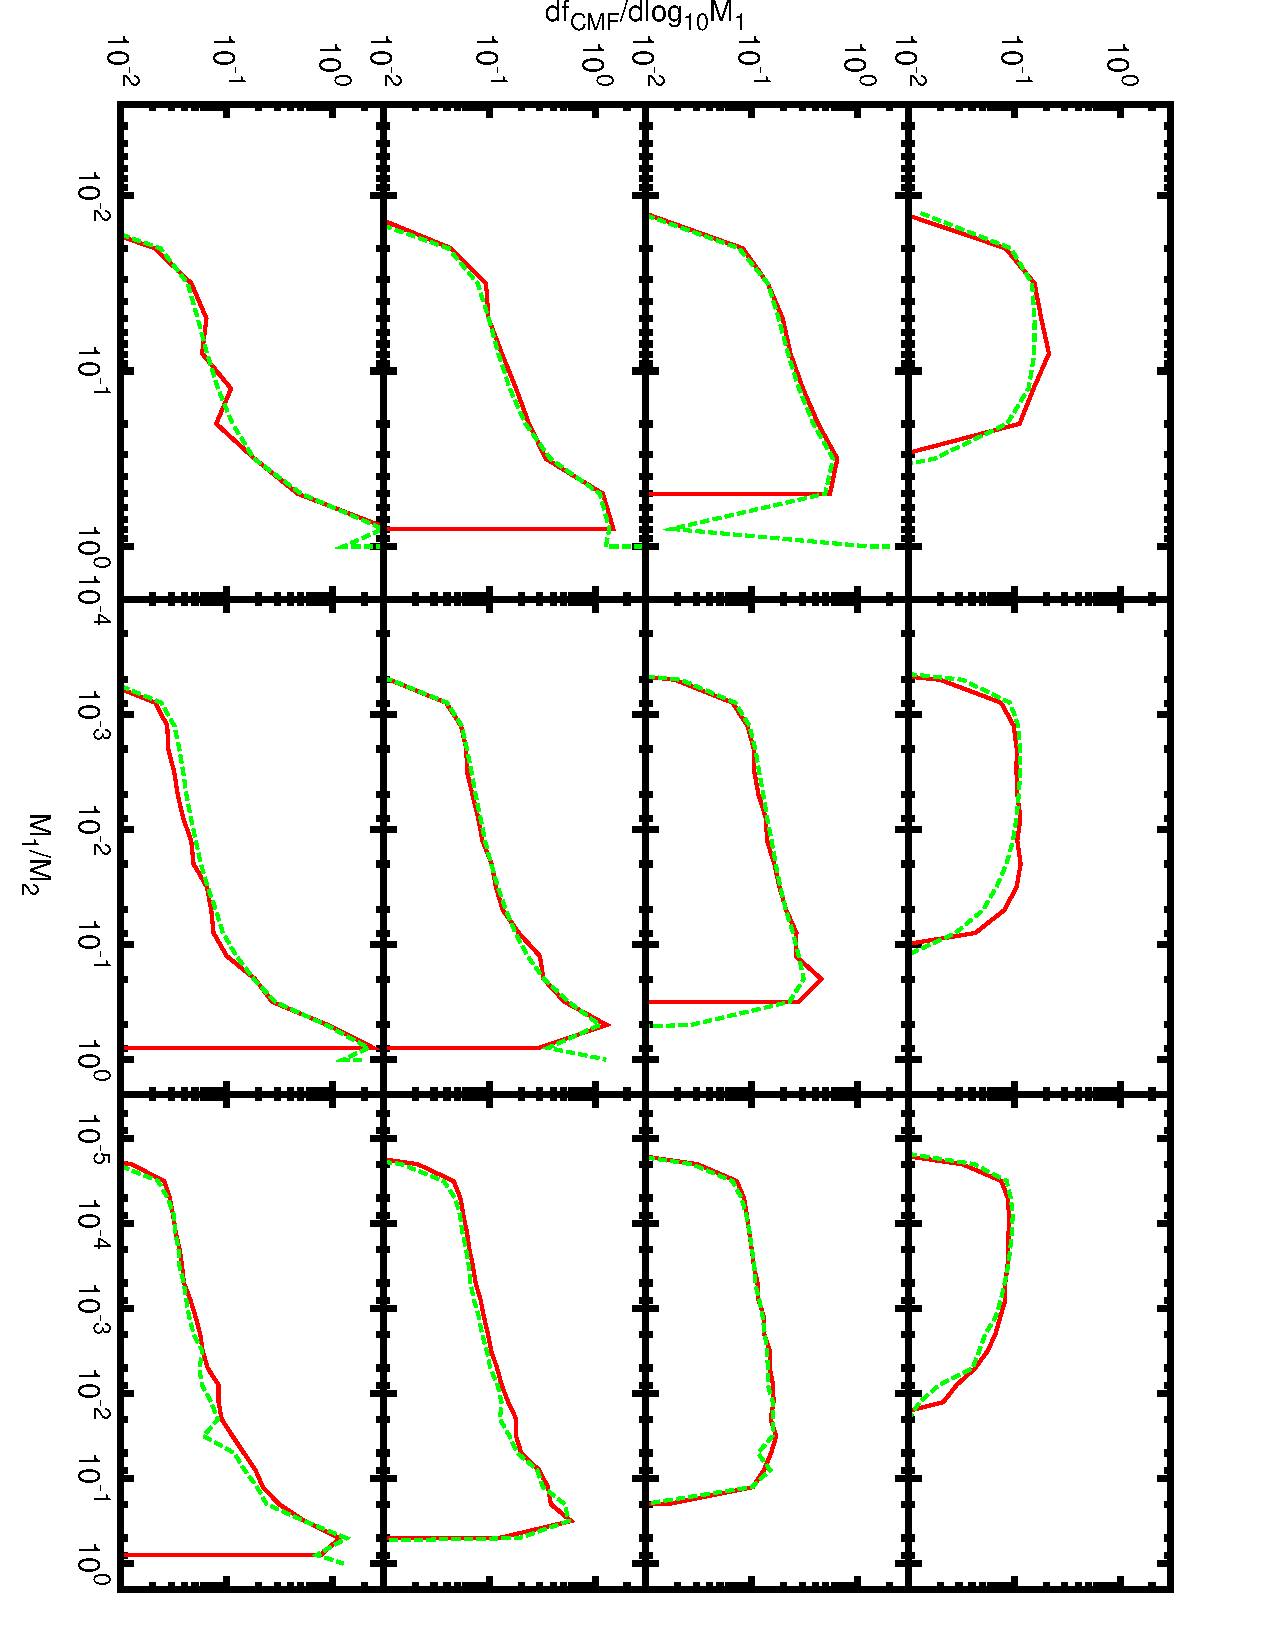
\includegraphics[height=160mm,angle=90]{../plots/progenitorMassFunction.pdf}
 \end{center}
 \caption{Progenitor mass functions at redshifts $z=0.5$, 1, 2 and 4 (bottom to top) for halos of mass $10^{12\pm0.151}$, $10^{13.5\pm0.151}$ and $10^{15\pm0.151}h^{-1}M_\odot$ (left to right) are shown. Green lines are measured from the Millennium Simulation, while red lines are computed using \glc's merger tree building routines (with the \cite{parkinson_generating_2008} branching algorithm and the \cite{cole_hierarchical_2000} tree building algorithm).}
 \label{fig:PCH_Progenitor_MFs}
\end{figure}

\subsubsection{Merger Tree Branching Modifiers}\label{sec:treeBranchingModifierMethod}

Additional methods for merger tree branching probability modifiers can be added using the {\normalfont \ttfamily treeBranchingModifierMethod} directive. The directive should contain a single argument, giving the name of a subroutine to be called to initialize the method. For example, the {\normalfont \ttfamily null} method is described by a directive:
\begin{verbatim}
 !# <treeBranchingModifierMethod>
 !#  <unitName>Merger_Tree_Branching_Modifiers_Null_Initialize</unitName>
 !# </treeBranchingModifierMethod>
\end{verbatim}
Here, {\normalfont \ttfamily Merger\_Tree\_Branching\_Modifiers\_Null\_Initialize} is the name of a subroutine which will be called to initialize the method. The initialization subroutine must have the following form:
\begin{verbatim}
 subroutine Method_Initialize(treeBranchingModifierMethod,Merger_Tree_Branching_Modifier_Get)
    type     (varying_string  ),          intent(in   ) :: treeBranchingModifierMethod
    procedure(double precision), pointer, intent(inout) :: Merger_Tree_Branching_Modifier_Get
    
    if (treeBranchingModifierMethod == 'myMethod') then
       Merger_Tree_Branching_Modifier_Get => My_Get
       .
       .
       .
    end if
    return
  end subroutine Method_Initialize
\end{verbatim}
where {\normalfont \ttfamily myMethod} is the name of this method as will be specified by the {\normalfont \ttfamily treeBranchingModifierMethod} input parameter. The procedure pointer {\normalfont \ttfamily Merger\_Tree\_Branching\_Modifier\_Get} must build and return the modifier to the branching probability as described below. The initialization subroutine should perform any other tasks required to initialize the module (such as reading parameters etc.).

The branching probability modifier function should have the interface:
\begin{verbatim}
  subroutine Merger_Tree_Branching_Modifier_Get(parentDelta,childSigma,parentSigma)
    double precision, intent(in) :: parentDelta,childSigma,parentSigma
    .
    .
    .
    return
  end subroutine Merger_Tree_Branching_Modifier_Get
\end{verbatim}
and should return the multiplicative modifier to the branching probability for the given {\normalfont \ttfamily parentDelta}, {\normalfont \ttfamily childSigma} and {\normalfont \ttfamily parentSigma}.

Currently defined merger tree branching probability modifier methods are:
\begin{description}
 \item [{\normalfont \ttfamily null}] Makes no modification;
 \item [{\normalfont \ttfamily Parkinson-Cole-Helly2008}] Modifies branching rates according to the algorithm of \cite{parkinson_generating_2008}.
\end{description}

\subsubsection{Merger Tree Building Mass Resolution}\label{sec:MergerTreeBuildMethodMassResolution}

Additional methods for the mass resolution to use when building merger trees can be added using the {\normalfont \ttfamily mergerTreesBuildMassResolution} directive. The directive should contain a single argument, giving the name of a subroutine to be called to initialize the method. For example, the {\normalfont \ttfamily fixed} method is described by a directive:
\begin{verbatim}
 !# <mergerTreesBuildMassResolution>
 !#  <unitName>Merger_Trees_Build_Mass_Resolution_Fixed_Initialize</unitName>
 !# </mergerTreesBuildMassResolution>
\end{verbatim}
Here, {\normalfont \ttfamily Merger\_Trees\_Build\_Mass\_Resolution\_Fixed\_Initialize} is the name of a subroutine which will be called to initialize the method. The initialization subroutine must have the following form:
\begin{verbatim}
 subroutine Method_Initialize(mergerTreesBuildMassResolutionMetod,Merger_Tree_Build_Mass_Resolution_Get)
    type(varying_string),          intent(in)    :: mergerTreesBuildMassResolutionMetod
    procedure(),          pointer, intent(inout) :: Merger_Tree_Build_Mass_Resolution_Get
    
    if (mergerTreesBuildMassResolutionMetod == 'myMethod') then
       Merger_Tree_Build_Mass_Resolution_Get => My_Merger_Tree_Build_Mass_Resolution
       .
       .
       .
    end if
    return
  end subroutine Method_Initialize
\end{verbatim}
where {\normalfont \ttfamily myMethod} is the name of this method as will be specified by the {\normalfont \ttfamily mergerTreesBuildMassResolutionMetod} input parameter. The procedure pointer {\normalfont \ttfamily Merger\_Tree\_Build\_Mass\_Resolution\_Get} must be set to point to a function which returns the mass resolution to use for a given tree as described below. The initialization subroutine should perform any other tasks required to initialize the module (such as reading parameters etc.).

The mass resolution function should have the form:
\begin{verbatim}
  double precision function Merger_Tree_Build_Mass_Resolution(thisTree)
    type(mergerTree), intent(in   ) :: thisTree
    .
    .
    .
    return
  end function Merger_Tree_Build_Mass_Resolution
\end{verbatim}
and should return the mass resolution to use when building {\normalfont \ttfamily thisTree}. Note that the base node in {\normalfont \ttfamily thisTree} will already be set.

Currently defined merger tree building mass resolution methods are:
\begin{description}
 \item [{\normalfont \ttfamily fixed}] Uses a fixed mass resolution for all trees.
 \item [{\normalfont \ttfamily scaled}] The resolution is set to a fraction of the tree base node mass (or a defined minimum, whichever is larger).
\end{description}

\subsubsection{Merger Tree Construction}\label{sec:MergerTreeConstruction}

Additional methods for merger tree construction can be added using the {\normalfont \ttfamily mergerTreeConstructMethod} directive. The directive should contain a single argument, giving the name of a subroutine to be called to initialize the method. For example, the {\normalfont \ttfamily build} method is described by a directive:
\begin{verbatim}
 !# <mergerTreeConstructMethod>
 !#  <unitName>Merger_Tree_Build_Initialize</unitName>
 !# </mergerTreeConstructMethod>
\end{verbatim}
Here, {\normalfont \ttfamily Merger\_Tree\_Build\_Initialize} is the name of a subroutine which will be called to initialize the method. The initialization subroutine must have the following form:
\begin{verbatim}
   subroutine Method_Initialize(mergerTreeConstructMethod,Merger_Tree_Construct)
    type(varying_string),          intent(in)    :: mergerTreeConstructMethod
    procedure(),          pointer, intent(inout) :: Merger_Tree_Construct
    
    if (mergerTreeConstructMethod == 'myMethod') then
       Merger_Tree_Construct => My_Do_Tabulate
       .
       .
       .
    end if
    return
  end subroutine Method_Initialize
\end{verbatim}
where {\normalfont \ttfamily myMethod} is the name of this method as will be specified by the {\normalfont \ttfamily mergerTreeConstructMethod} input parameter. The procedure pointer {\normalfont \ttfamily Merger\_Tree\_Construct} must be set to point to a function which returns a fully constructed merger tree as described below. The initialization subroutine should perform any other tasks required to initialize the module (such as reading parameters etc.).

The construction subroutine should have the following form:
\begin{verbatim}
  subroutine Merger_Tree_Construct_Do(thisTree,skipTree)
    type(mergerTree), intent(inout) :: thisTree
    logical,          intent(in)    :: skipTree
    .
    .
    .
    return
  end subroutine Merger_Tree_Construct_Do
\end{verbatim}
and should return a full merger tree in {\normalfont \ttfamily thisTree}, unless {\normalfont \ttfamily skipTree} is true, in which case this tree will be skipped (i.e. not evolved or output) and so it suffices to merely allocate the base node---there is no need to create the entire tree (although it is permissible to do so)---and update any internal data (e.g. a count of trees constructed) as required. The tree must have at least masses, times and parent/child/sibling links created. Other properties (e.g. spins) can be optionally included also. By default, the tree is assumed to be ``uninitialized'', such that the merger tree initialization function will be called prior to the tree being evolve. If the tree construction method returns a fully initialized tree it should set {\normalfont \ttfamily thisTree\%initialized=.true.}.

Currently defined merger tree construction methods are:
\begin{description}
 \item [{\normalfont \ttfamily build}] Generates a set of halo masses distributed between {\normalfont \ttfamily mergerTreeBuildHaloMassMinimum} and {\normalfont \ttfamily mergerTreeBuildHaloMassMaximum} (with {\normalfont \ttfamily mergerTreeBuildTreesPerDecade} halos per decade of mass) at redshift {\normalfont \ttfamily mergerTreeBuildTreesBaseRedshift}, or with masses read from a file, and then uses the selected merger tree build method (see \S\ref{sec:methodsMergerTreeBuilder}) to build trees from these base nodes;
 \item [{\normalfont \ttfamily read}] Reads merger tree data from an HDF5 file (see \S\ref{sec:MergerTreeFiles}). The file to read is specified by the {\normalfont \ttfamily [mergerTreeReadFileName]} parameter.
 \item [{\normalfont \ttfamily smoothAccretion}] Constructs a branchless merger tree with a smooth accretion history using the selected mass accretion history method (see \S\ref{sec:methodsDarkMatterHaloMassAccretionHistory}). See \S\ref{sec:SmoothAccretion} for details.
 \item [{\normalfont \ttfamily stateRestore}] Intended primarily for debugging purposes, this method will restore a tree whose complete internal state was written to file. See \S\ref{sec:TreeConstructStateRestore} for details of how to use this method.
 \item [{\normalfont \ttfamily fullySpecified}] Intended primarily for constructing test cases, this method allows the full state of the merger tree (and all components of nodes) to be specified via an XML document. See \S\ref{sec:TreeConstructFullySpecified} for details of how to use this method.
\end{description}

\subsubsection{Non-linear Matter Power Spectrum}\index{power spectrum!non-linear}

Additional methods for the non-linear matter power spectrum can be added using the {\normalfont \ttfamily powerSpectrumNonlinearMethod} directive. The directive should contain a single argument, giving the name of a subroutine to be called to initialize the method. For example, the {\normalfont \ttfamily Peacock-Dodds1996} method is described by a directive:
\begin{verbatim}
  !# <powerSpectrumNonlinearMethod>
  !#  <unitName>Nonlinear_Power_Spectrum_Power_Law_Initialize</unitName>
  !# </powerSpectrumNonlinearMethod>
\end{verbatim}
Here, {\normalfont \ttfamily Power\_Spectrum\_Nonlinear\_PeacockDodds1996\_Initialize} is the name of a subroutine which will be called to initialize the method. The initialization subroutine must have the following form:
\begin{verbatim}
  subroutine Method_Initialize(powerSpectrumNonlinearMethod,Power_Spectrum_Nonlinear_Get)
    implicit none
    type     (varying_string  ),          intent(in   ) :: powerSpectrumNonlinearMethod
    procedure(double precision), pointer, intent(inout) :: Power_Spectrum_Nonlinear_Get
    
    if (powerSpectrumNonlinearMethod == 'myMethod') then
       Power_Spectrum_Nonlinear_Get => My_Get
       .
       .
       .
    end if
    return
  end subroutine Method_Initialize
\end{verbatim}
where {\normalfont \ttfamily myMethod} is the name of this method as will be specified by the {\normalfont \ttfamily powerSpectrumNonlinearMethod} input parameter. The procedure pointer {\normalfont \ttfamily Power\_Spectrum\_Nonlinear\_Get} must be set to point to a subroutine which computes the non-linear matter power spectrum as described below. The initialization subroutine should perform any other tasks required to initialize the module (such as reading parameters etc.).

The non-linear matter power spectrum function must have the form:
\begin{verbatim}
   double precision function Nonlinear_Power_Spectrum(wavenumber,time)
    implicit none
    double precision, intent(in   ) :: wavenumber,time
    .
    .
    .
    return
   end subroutine Nonlinear_Power_Spectrum
\end{verbatim}
The function must return the non-linear matter power spectrum, $P_{\mathrm nl}(k)$, at the requested {\normalfont \ttfamily wavenumber} (in units of Mpc$^{-1}$) and {\normalfont \ttfamily time} (in units of Gyr).

Currently defined non-linear matter power spectrum methods are:
\begin{description}
 \item [{\normalfont \ttfamily linear}] Simply returns the linear matter power spectrum. Intended primarily for testing purposes.
 \item [{\normalfont \ttfamily Peacock-Dodds1996}] Uses the fitting function of \cite{peacock_non-linear_1996} to compute the non-linear matter power spectrum.
 \item [{\normalfont \ttfamily CosmicEmu}] Utilizes the cosmic emulator (``CosmicEmu'') code of \cite{lawrence_coyote_2010} to compute the non-linear matter power spectrum.
\end{description}

\subsubsection{Chemical Reaction Rates}

Additional methods for chemical species reaction rates can be added using the {\normalfont \ttfamily chemicalReactionRatesMethods} directive. Note that more than one method can be specified in which cases rates are cumulative over all selected methods. The directive should contain a single argument, giving the name of a subroutine to be called to initialize the method. For example, the {\normalfont \ttfamily hydrogenNetwork} method is described by a directive:
\begin{verbatim}
  !# <chemicalReactionRatesMethods>
  !#  <unitName>Chemical_Hydrogen_Rates_Initialize</unitName>
  !# </chemicalReactionRatesMethods>
\end{verbatim}
Here, {\normalfont \ttfamily Chemical\_Hydrogen\_Rates\_Initialize} is the name of a subroutine which will be called to initialize the method. The initialization subroutine must have the following form:
\begin{verbatim}
  subroutine Method_Initialize(chemicalReactionRatesMethods)
    implicit none
    type(varying_string), intent(in) :: chemicalReactionRatesMethods
    
    if (chemicalReactionRatesMethods == 'myMethod') then
       ratesSelected = .true.
       .
       .
       .
    end if
    return
  end subroutine Method_Initialize
\end{verbatim}
where {\normalfont \ttfamily myMethod} is the name of this method as will be specified by the {\normalfont \ttfamily chemicalReactionRatesMethods} input parameter. The {\normalfont \ttfamily ratesSelected} variable is set to true if the method is active and will be checked on all subsequent calls to the module such that rates are computed only if {\normalfont \ttfamily ratesSelected} is true. The initialization subroutine should perform any other tasks required to initialize the module (such as reading parameters etc.).

The method must provide a subroutine to compute the chemical reaction rates. This subroutine is specified by the {\normalfont \ttfamily chemicalRatesCompute} directive. The directive should contain a single argument, giving the name of a subroutine to be called to compute rates. For example, the {\normalfont \ttfamily hydrogenNetwork} method uses:
\begin{verbatim}
  !# <chemicalRatesCompute>
  !#  <unitName>Chemical_Hydrogen_Rates_Compute</unitName>
  !# </chemicalRatesCompute> 
\end{verbatim}
Here, {\normalfont \ttfamily Chemical\_Hydrogen\_Rates\_Compute} is the name of a subroutine which will be called to compute the rates. The rates subroutine must have the following form:
\begin{verbatim}
  subroutine Compute_Rates(temperature,chemicalDensity,radiation,chemicalRates)
    implicit none
    type(chemicalAbundancesStructure), intent(in)    :: chemicalDensity
    double precision,                  intent(in)    :: temperature
    type(radiationStructure),          intent(in)    :: radiation
    type(chemicalAbundancesStructure), intent(inout) :: chemicalRates

    ! Exit immediately if this method is not active.
    if (.not.ratesSelected) return

    ! Compute rates for all species present.
    .
    .
    .
    return
  end subroutine Compute_Rates
\end{verbatim}
Here, {\normalfont \ttfamily temperature} is the temperature of the gas, {\normalfont \ttfamily chemicalDensity} provides the densities (in cm$^{-3}$) of all chemicals, the radiation field is described by the {\normalfont \ttfamily radiation} object and any reaction rates should be \emph{added to} the {\normalfont \ttfamily chemicalRates} object in units of cm$^{-3}$ s$^{-1}$.

Currently defined chemical reaction rate methods are:
\begin{description}
 \item [{\normalfont \ttfamily null}] A null method which does not affect any rates.
 \item [{\normalfont \ttfamily hydrogenNetwork}] Computes rates using the network of reactions and fitting functions from \cite{abel_modeling_1997} and \cite{tegmark_small_1997}.
\end{description}

\subsubsection{Population III Supernovae}

Additional methods for Population III supernovae can be added using the {\normalfont \ttfamily supernovaePopIIIMethod} directive. The directive should contain a single argument, giving the name of a subroutine to be called to initialize the method. For example, the {\normalfont \ttfamily Heger-Woosley2002} method is described by a directive:
\begin{verbatim}
  !# <supernovaePopIIIMethod>
  !#  <unitName>Supernovae_Population_III_HegerWoosley_Initialize</unitName>
  !# </supernovaePopIIIMethod>
\end{verbatim}
Here, {\normalfont \ttfamily Supernovae\_Population\_III\_HegerWoosley\_Initialize} is the name of a subroutine which will be called to initialize the method. The initialization subroutine must have the following form:
\begin{verbatim}
  subroutine Method_Initialize(supernovaePopIIIMethod,SNePopIII_Cumulative_Energy_Get)
    implicit none
    type(varying_string),          intent(in)    :: supernovaePopIIIMethod
    procedure(),          pointer, intent(inout) :: SNePopIII_Cumulative_Energy_Get
    
    if (supernovaePopIIIMethod == 'myMethod') then
       SNePopIII_Cumulative_Energy_Get => My_SNePopIII_Cumulative_Energy_Get
       .
       .
       .
    end if
    return
  end subroutine Method_Initialize
\end{verbatim}
where {\normalfont \ttfamily myMethod} is the name of this method as will be specified by the {\normalfont \ttfamily supernovaePopIIIMethod} input parameter. The procedure pointer {\normalfont \ttfamily SNePopIII\_Cumulative\_Energy\_Get} must be set to point to a function which returns the cumulative energy input from Population III supernovae as described below. The initialization subroutine should perform any other tasks required to initialize the module (such as reading parameters etc.).

The functions must have the form:
\begin{verbatim}
   double precision function PopIII_Cumulative_Energy(initialMass,age,metallicity)
    implicit none
    double precision, intent(in) :: initialMass,age,metallicity
    .
    .
    .
    return
   end function PopIII_Cumulative_Energy 
\end{verbatim}
This function must return the cumulative energy (in $M_\odot$ (km/s)$^2$) from Population III supernovae resulting from a star with given {\normalfont \ttfamily initialMass} and {\normalfont \ttfamily metallicity} after a time {\normalfont \ttfamily age}.

Currently defined population III supernovae methods are:
\begin{description}
 \item [{\normalfont \ttfamily Heger-Woosley2002}] Computes the energy input from the pair-instability results of \cite{heger_nucleosynthetic_2002}.
\end{description}

\subsubsection{Power Spectrum Variance Window Function}\label{sec:PowerSpectrumWindowFunction}

Additional methods for the window function used to compute variance from the power spectrum can be added using the {\normalfont \ttfamily powerSpectrumWindowFunctionMethod} directive. The directive should contain a single argument, giving the name of a subroutine to be called to initialize the method. For example, the {\normalfont \ttfamily topHat} method is described by a directive:
\begin{verbatim}
  !# <powerSpectrumWindowFunctionMethod>
  !#  <unitName>Power_Spectrum_Window_Functions_Top_Hat_Initialize</unitName>
  !# </powerSpectrumWindowFunctionMethod>
\end{verbatim}
Here, {\normalfont \ttfamily Power\_Spectrum\_Window\_Functions\_Top\_Hat\_Initialize} is the name of a subroutine which will be called to initialize the method. The initialization subroutine must have the following form:
\begin{verbatim}
  subroutine Method_Initialize(powerSpectrumWindowFunctionMethod,Power_Spectrum_Window_Function_Get)
    implicit none
    type     (varying_string  ),          intent(in   ) :: powerSpectrumWindowFunctionMethod
    procedure(double precision), pointer, intent(inout) :: Power_Spectrum_Window_Function_Get
    procedure(double precision), pointer, intent(inout) :: Power_Spectrum_Window_Function_Wavenumber_Maximum_Get
    
    if (powerSpectrumWindowFunctionMethod == 'myMethod') then
       Power_Spectrum_Window_Function_Get                    => My_Window_Function
       Power_Spectrum_Window_Function_Wavenumber_Maximum_Get => My_Window_Function_Maximum_Wavelength
       .
       .
       .
    end if
    return
  end subroutine Method_Initialize
\end{verbatim}
where {\normalfont \ttfamily myMethod} is the name of this method as will be specified by the {\normalfont \ttfamily powerSpectrumWindowFunctionMethod} input parameter. The procedure pointers {\normalfont \ttfamily Power\_Spectrum\_Window\_Function\_Get}, and {\normalfont \ttfamily Power\_Spectrum\_Window\_Function\_Wavenumber\_Maximum\_Get} must be set to point to functions which return the window function for a given wavenumber and mass, and the maximum wavenumber for which that window function is non-zero respectively. The initialization subroutine should perform any other tasks required to initialize the module (such as reading parameters etc.).

The window function function must have the form:
\begin{verbatim}
   subroutine Power_Spectrum_Window_Function(wavenumber,smoothingMass)
    implicit none
    double precision, intent(in   ) :: wavenumber,smoothingMass
     .
    .
    .
    return
   end subroutine Power_Spectrum_Window_Function
\end{verbatim}
The function should return the window function for the specified {\normalfont \ttfamily wavenumber} (given in Mpc$^{-1}$) and the given {\normalfont \ttfamily smoothingMass} (given in $M_\odot$).

The window function maximum wavenumber function must have the form:
\begin{verbatim}
   subroutine Power_Spectrum_Window_Function_Wavenumber_Maximum(smoothingMass)
    implicit none
    double precision, intent(in   ) :: smoothingMass
     .
    .
    .
    return
   end subroutine Power_Spectrum_Window_Function_Wavenumber_Maximum
\end{verbatim}
The function should return the largest wavenumber for which the window function is non-zero for the given {\normalfont \ttfamily smoothingMass} (given in $M_\odot$). If the window function is non-zero as $k\rightarrow\infty$ then a suitably large value (e.g. $10^{30}$Mpc$^{-1}$) should be returned.

Currently defined power spectrum variance window function methods are:
\begin{description}
 \item [{\normalfont \ttfamily topHat}] The window function is a top-hat in real-space.
 \item [{\normalfont \ttfamily kSpaceSharp}] The window function is a top-hat in $k$-space.
 \item [{\normalfont \ttfamily topHatKSpaceSharpHybrid}] A convolution of top-hat in real space and top-hat in $k$-space window functions.
\end{description}

\subsubsection{Primordial Power Spectrum}

Additional methods for the primordial power spectrum can be added using the {\normalfont \ttfamily powerSpectrumMethod} directive. The directive should contain a single argument, giving the name of a subroutine to be called to initialize the method. For example, the {\normalfont \ttfamily powerLaw} method is described by a directive:
\begin{verbatim}
  !# <powerSpectrumMethod>
  !#  <unitName>CDM_Primordial_Power_Spectrum_Power_Law_Initialize</unitName>
  !# </powerSpectrumMethod>
\end{verbatim}
Here, {\normalfont \ttfamily CDM\_Primordial\_Power\_Spectrum\_Power\_Law\_Initialize} is the name of a subroutine which will be called to initialize the method. The initialization subroutine must have the following form:
\begin{verbatim}
  subroutine Method_Initialize(powerSpectrumMethod,Power_Spectrum_Tabulate)
    implicit none
    type(varying_string),          intent(in)    :: powerSpectrumMethod
    procedure(),          pointer, intent(inout) :: Power_Spectrum_Tabulate
    
    if (powerSpectrumMethod.eq.'myMethod') then
       Power_Spectrum_Tabulate => My_Do_Tabulate
       .
       .
       .
    end if
    return
  end subroutine Method_Initialize
\end{verbatim}
where {\normalfont \ttfamily myMethod} is the name of this method as will be specified by the {\normalfont \ttfamily powerSpectrumMethod} input parameter. The procedure pointer {\normalfont \ttfamily Power\_Spectrum\_Tabulate} must be set to point to a subroutine which tabulates the power spectrum as described below. The initialization subroutine should perform any other tasks required to initialize the module (such as reading parameters etc.).

The tabulation subroutine must have the form:
\begin{verbatim}
   subroutine Power_Spectrum_Tabulate(wavenumber,powerSpectrumNumberPoints,powerSpectrumLogWavenumber,powerSpectrumLogP)
    implicit none
    double precision,                            intent(in)    :: wavenumber
    double precision, allocatable, dimension(:), intent(inout) :: powerSpectrumLogWavenumber,powerSpectrumLogP
    integer,                                     intent(out)   :: powerSpectrumNumberPoints
    .
    .
    .
    return
   end subroutine Power_Spectrum_Tabulate
\end{verbatim}
The subroutine must tabulate the natural log of the power spectrum in array {\normalfont \ttfamily powerSpectrumLogP()} as a function of the natural log of wavenumber {\normalfont \ttfamily powerSpectrumLogWavenumber()} (these arrays must be allocated to the correct size, and may be prevously allocated, therefore requiring a deallocation). The number of tabulated points should be returned in {\normalfont \ttfamily powerSpectrumNumberPoints}. The subroutine should ensure that the currently requested {\normalfont \ttfamily wavenumber} is within the range of the tabulated function (preferably with some buffer).

Currently defined power spectrum methods are:
\begin{description}
 \item [{\normalfont \ttfamily powerLaw}] The power spectrum is assumed to be a power law, possibly with a running index. It is defined by
\begin{equation}
 P(k)\propto k^{n_{\mathrm s} + \ln(k/k_{\mathrm ref}) [\d n /\d\ln k]},
\end{equation}
where the parameters are specified by input parameters $n_{\mathrm s}\equiv${\normalfont \ttfamily powerSpectrumIndex}, $k_{\mathrm ref}\equiv${\normalfont \ttfamily powerSpectrumReferenceWavenumber} and $\d n / \d \ln k \equiv${\normalfont \ttfamily powerSpectrumRunning}.
\end{description}

\subsubsection{Radiation Components}\index{radiation}\label{sec:radiationComponents}

Radiation components (i.e. types of radiation field that may be added to any radiation object; see \S\ref{sec:RadiationSubsystem}) are defined using a combination of several directives: {\normalfont \ttfamily radiationLabel}, {\normalfont \ttfamily radiationSet}, {\normalfont \ttfamily radiationTemperature} and {\normalfont \ttfamily radiationFlux}. For example, the cosmic microwave background radiation component is defined by the following set of directives:
\begin{verbatim}
  !# <radiationLabel>
  !#  <label>CMB</label>
  !# </radiationLabel>

  !# <radiationSet>
  !#  <unitName>Radiation_Set_CMB</unitName>
  !#  <label>CMB</label>
  !# </radiationSet>

  !# <radiationTemperature>
  !#  <unitName>Radiation_Temperature_CMB</unitName>
  !#  <label>CMB</label>
  !# </radiationTemperature>

  !# <radiationFlux>
  !#  <unitName>Radiation_Flux_CMB</unitName>
  !#  <label>CMB</label>
  !# </radiationFlux>
\end{verbatim}
The first of these, {\normalfont \ttfamily radiationLabel}, should contain a single element, {\normalfont \ttfamily label}, which gives a label that will be used to identify this component, both in other directives and also in the internal parameters used to select this radiation component (e.g. in this case, a parameter {\normalfont \ttfamily radiationTypeCMB} will be available within \glc\ to select the cosmic microwave background component). The other directives must all specify the same {\normalfont \ttfamily label} element and additional give, in a {\normalfont \ttfamily unitName} element, the name of a function/subroutine to be called to perform the relevant calculation.

The {\normalfont \ttfamily radiationSet} directive must specify a subroutine with the following template:
\begin{verbatim}
  subroutine Radiation_Set(componentMatched,thisNode,radiationProperties)
   implicit none
   logical,          intent(in)                               :: componentMatched
   type(treeNode),   intent(inout), pointer                   :: thisNode
   double precision, intent(inout), allocatable, dimension(:) :: radiationProperties

   if (.not.componentMatched) return
   .
   .
   .
   return
  end subroutine Radiation_Set
\end{verbatim}
If {\normalfont \ttfamily componentMatched} is true, then the subroutine should set the radiation component, otherwise it should exit immediately. If the radiation component is to be set, then the routine can allocate the {\normalfont \ttfamily radiationProperties} array as necessary to store any data needed to specify the radiation field. These data should then be set using, if necessary, any relevant information from {\normalfont \ttfamily thisNode}.

The {\normalfont \ttfamily radiationTemperature} directive should specify a subroutine with the following template:
\begin{verbatim}
  subroutine Radiation_Temperature(requestedType,ourType,radiationProperties,radiationTemperature,radiationType)
   implicit none
   integer,          intent(in)                            :: requestedType,ourType
   double precision, intent(in),              dimension(:) :: radiationProperties
   double precision, intent(inout)                         :: radiationTemperature
   integer,          intent(in),    optional, dimension(:) :: radiationType

   if (requestedType /= ourType) return
   if (present(radiationType)) then
      if (all(radiationType /= ourType)) return
   end if
   .
   .
   .
   return
  end subroutine Radiation_Temperature
\end{verbatim}
The tests in the above should always be included so that the subroutine exits immediately if the component type is not active or not requested. Once these tests have been made, the subroutine should set the temperature (in units of Kelvin) of the radiation field (if applicable).

The {\normalfont \ttfamily radiationFlux} directive should specify a subroutine with the following template:
\begin{verbatim}
  subroutine Radiation_Flux(requestedType,ourType,radiationProperties,wavelength,radiationFlux,radiationType)
    implicit none
    integer,          intent(in)                           :: requestedType,ourType
    double precision, intent(in)                           :: wavelength
    double precision, intent(in),             dimension(:) :: radiationProperties
    double precision, intent(inout)                        :: radiationFlux
    integer,          intent(in),   optional, dimension(:) :: radiationType

    if (requestedType /= ourType) return
    if (present(radiationType)) then
       if (all(radiationType /= ourType)) return
    end if
    .
    .
    .
    return
  end subroutine Radiation_Flux
\end{verbatim}
The tests in the above should always be included so that the subroutine exits immediately if the component type is not active or not requested. Once these tests have been made, the subroutine should add the flux (in units of ergs cm$^2$ s$^{-1}$ Hz$^{-1}$ ster$^{-1}$) at the specified {\normalfont \ttfamily wavelength} (in units of \AA) of the radiation field to that in {\normalfont \ttfamily radiationFlux}.

Currently defined radiation component types are:
\begin{description}
 \item [{\normalfont \ttfamily null}] A null component with no radiation.
 \item [{\normalfont \ttfamily CMB}] The cosmic microwave background, assumed to be a perfect blackbody spectrum with a temperature equal to {\normalfont \ttfamily [T\_CMB]}$(1+z)$.
 \item [{\normalfont \ttfamily IGB}] The intergalactic background light, set using the method selected by {\normalfont \ttfamily [radiationIntergalacticBackgroundMethod]; see \S\ref{sec:radiationIGB}}.
\end{description}

\subsubsection{Radiation Components: Intergalactic Background}\label{sec:radiationIGB}

Additional methods for the intergalactic background radiation component can be added using the {\normalfont \ttfamily radiationIntergalacticBackgroundMethod} directive. The directive should contain a single argument, giving the name of a subroutine to be called to initialize the method. For example, the {\normalfont \ttfamily file} method is described by a directive:
\begin{verbatim}
 !# <radiationIntergalacticBackgroundMethod>
 !#  <unitName>Radiation_IGB_File_Initialize</unitName>
 !# </radiationIntergalacticBackgroundMethod>
\end{verbatim}
Here, {\normalfont \ttfamily Radiation\_IGB\_File\_Initialize} is the name of a subroutine which will be called to initialize the method. The initialization subroutine must have the following form:
\begin{verbatim}
  subroutine Method_Initialize(radiationIntergalacticBackgroundMethod,Radiation_Set_Intergalactic_Background_Do,Radiation_Flux_Intergalactic_Background_Do)
    implicit none
    type(varying_string),          intent(in)    :: radiationIntergalacticBackgroundMethod
    procedure(),          pointer, intent(inout) :: Radiation_Set_Intergalactic_Background_Do,Radiation_Flux_Intergalactic_Background_Do
    
    if (radiationIntergalacticBackgroundMethod == 'myMethod') then
      Radiation_Set_Intergalactic_Background_Do  => My_Method_Set
      Radiation_Flux_Intergalactic_Background_Do => My_Method_Flux
    end if
    return
  end subroutine Method_Initialize
\end{verbatim}
where {\normalfont \ttfamily myMethod} is the name of this method as will be specified by the {\normalfont \ttfamily radiationIntergalacticBackgroundMethod} input parameter. The procedure pointers {\normalfont \ttfamily Radiation\_Set\_Intergalactic\_Background\_Do} and {\normalfont \ttfamily Radiation\_Flux\_Intergalactic\_Background\_Do} must be set to point to subroutines which set the radiation field and return its flux as described below. The initialization subroutine should perform any other tasks required to initialize the module (such as reading parameters etc.).

The set subroutine must have the form:
\begin{verbatim}
  subroutine My_Method_Set(thisNode,radiationProperties)
    implicit none
    type(treeNode),   intent(inout), pointer                   :: thisNode
    double precision, intent(inout), allocatable, dimension(:) :: radiationProperties

    return
  end subroutine My_Method_Set
\end{verbatim}
and should set the radiation component as described in \S\ref{sec:radiationComponents}. The flux subroutine must have the form:
\begin{verbatim}
   subroutine My_Method_Flux(radiationProperties,wavelength,radiationFlux)
    implicit none
    double precision, intent(in)                 :: wavelength
    double precision, intent(in),   dimension(:) :: radiationProperties
    double precision, intent(inout)              :: radiationFlux

    return
   end subroutine My_Method_Flux
\end{verbatim}
and should increment {\normalfont \ttfamily radiationFlux} as described in \S\ref{sec:radiationComponents}.

Currently defined intergalactic background radiation methods are:
\begin{description}
 \item [{\normalfont \ttfamily file}] The intergalatic background radiation field, specified as a function of cosmic time, is read from a file. The flux is determined by linearly interpolating to the required time and wavelength. The XML file to read is specified by {\normalfont \ttfamily [radiationIGBFileName]}. An example of the required file structure is:
 \begin{verbatim}
<spectrum>
  <URL>http://adsabs.harvard.edu/abs/1996ApJ...461...20H</URL>
  <description>Cosmic background radiation spectrum from quasars alone.</description>
  <reference>Haardt, F. &amp; Madau, P. 1996, ApJ, 461, 20</reference>
  <source>Francesco Haardt on Aug 6 2005, via Cloudy 08.00</source>
  <wavelengths>
    <datum>0.0002481</datum>
    <datum>0.001489</datum>
    .
    .
    .
    <units>Angstroms</units>
  </wavelengths>
  <spectra>
    <datum>7.039E-49</datum>
    <datum>8.379E-48</datum>
    <datum>1.875E-39</datum>
    <datum>7.583E-38</datum>
    .
    .
    .
    <redshift>0</redshift>
    <units>erg cm^-2 s^-1 Hz^-1 sr^-1</units>
  </spectra>
</spectrum>
 \end{verbatim}
\end{description}
The optional {\normalfont \ttfamily URL}, {\normalfont \ttfamily description}, {\normalfont \ttfamily reference} and {\normalfont \ttfamily source} elements can be used to give the provenance of the data. The {\normalfont \ttfamily wavelengths} element should contain a set of {\normalfont \ttfamily datum} elements each containing a wavelength (in increasing order) at which the spectrum will be tabulated. Wavelengths must be given in Angstroms. Multiple {\normalfont \ttfamily spectra} elements can be given, each specifying the spectrum at a redshift as given in the {\normalfont \ttfamily redshift} element. Each {\normalfont \ttfamily spectra} element must contain an array of {\normalfont \ttfamily datum} elements that gives the spectrum at each wavelength listed in the {\normalfont \ttfamily wavelength} element. Spectra must be in units of erg cm$^{-2}$ s$^{-1}$ Hz$^{-1}$ sr$^{-1}$.

\subsubsection{Ram Pressure Mass Loss Rates in Disks/Spheroids}

Additional methods for computing ram pressure induced mass loss rates in disks/spheroids can be added using the {\normalfont \ttfamily ramPressureStrippingMassLossRate(Disks|Spheroids)Method} directive. The directive should contain a single argument, giving the name of a subroutine to be called to initialize the method. For example, the {\normalfont \ttfamily simple} method for disks is described by a directive:
\begin{verbatim}
 !# <ramPressureStrippingMassLossRateDisksMethod>
 !#  <unitName>Ram_Pressure_Stripping_Mass_Loss_Rate_Disks_Simple_Init</unitName>
 !# </ramPressureStrippingMassLossRateDisksMethod>
\end{verbatim}
Here, {\normalfont \ttfamily Ram\_Pressure\_Stripping\_Mass\_Loss\_Rate\_Disks\_Simple\_Init} is the name of a subroutine which will be called to initialize the method. The initialization subroutine must have the following form:
\begin{verbatim}
  subroutine Method_Initialize(ramPressureStrippingMassLossRateDisksMethod,Ram_Pressure_Stripping_Mass_Loss_Rate_Disk_Get)
    implicit none
    type(varying_string),          intent(in)    :: starFormationTimescaleDisksMethod
    procedure(),          pointer, intent(inout) :: Ram_Pressure_Stripping_Mass_Loss_Rate_Disk_Get
    
    if (ramPressureStrippingMassLossRateDisksMethod == 'myMethod') Ram_Pressure_Stripping_Mass_Loss_Rate_Disk_Get => My_Ram_Pressure_Stripping_Mass_Loss_Rate_Disk_Get
    return
  end subroutine Method_Initialize
\end{verbatim}
where {\normalfont \ttfamily myMethod} is the name of this method as will be specified by the {\normalfont \ttfamily ramPressureStrippingMassLossRate(Disks|Spheroids)Method} input parameter. The procedure pointer {\normalfont \ttfamily Ram\_Pressure\_Stripping\_Mass\_Loss\_Rate\_(Disk|Spheroid)\_Get} must be set to point to a function which returns mass loss rate due to ram pressure as described below. The initialization subroutine should perform any other tasks required to initialize the module (such as reading parameters etc.).

The mass loss rate function must have the form:
\begin{verbatim}
 double precision function Ram_Pressure_Stripping_Mass_Loss_Rate_Disk_Get(thisNode)
    implicit none
    type(treeNode), intent(in) :: thisNode
    .
    .
    .
    return
 end function Ram_Pressure_Stripping_Mass_Loss_Rate_Disk_Get
\end{verbatim}
The function must return the mass loss rate induced by ram pressure forces (in units of $M_\odot$/Gyr) for the disk/spheroid in {\normalfont \ttfamily thisNode}.

Currently defined ram pressure mass loss rate methods are:
\begin{description}
 \item [\hyperlink{ram_pressure_stripping.mass_loss_rate.disks.simple.F90:ram_pressure_stripping_mass_loss_rate_disks_simple:ram_pressure_stripping_mass_loss_rate_disk_simple}{{\normalfont \ttfamily simple}}] The mass loss rate scales in proportion to the ratio of ram pressure and gravitational restoring forces;
 \item [\hyperlink{ram_pressure_stripping.mass_loss_rate.disks.null.F90:ram_pressure_stripping_mass_loss_rate_disks_null:ram_pressure_stripping_mass_loss_rate_disk_null}{{\normalfont \ttfamily null}}] The mass loss rate is assumed to be always zero.
\end{description}

\subsubsection{Satellite Merging Mass Movements}

Additional methods for the satellite merging mass movements can be added using the {\normalfont \ttfamily satelliteMergingMassMovementsMethod} directive. The directive should contain a single argument, giving the name of a subroutine to be called to initialize the method. For example, the {\normalfont \ttfamily simple} method is described by a directive:
\begin{verbatim}
 !# <satelliteMergingMassMovementsMethod>
 !#  <unitName>Satellite_Merging_Mass_Movements_Simple_Initialize</unitName>
 !# </satelliteMergingMassMovementsMethod>
\end{verbatim}
Here, {\normalfont \ttfamily Satellite\_Merging\_Mass\_Movements\_Simple\_Initialize} is the name of a subroutine which will be called to initialize the method. The initialization subroutine must have the following form:
\begin{verbatim}
  subroutine Method_Initialize(satelliteMergingMassMovementsMethod,Satellite_Merging_Mass_Movement_Get)
    implicit none
    type(varying_string),          intent(in)    :: satelliteMergingMassMovementsMethod
    procedure(),          pointer, intent(inout) :: Satellite_Merging_Mass_Movement_Get
    
    if (satelliteMergingMassMovementsMethod == 'simple') Satellite_Merging_Mass_Movement_Get => My_Method_Get
    return
  end subroutine Method_Initialize
\end{verbatim}
where {\normalfont \ttfamily myMethod} is the name of this method as will be specified by the {\normalfont \ttfamily satelliteMergingMassMovementsMethod} input parameter. The procedure pointer {\normalfont \ttfamily Satellite\_Merging\_Mass\_Movement\_Get} must be set to point to a function which sets the mass movement descriptors as described below. The initialization subroutine should perform any other tasks required to initialize the module (such as reading parameters etc.).

The mass movement subroutine must have the form:
\begin{verbatim}
  subroutine My_Method_Get(thisNode,gasMovesTo,starsMoveTo,hostGasMovesTo,hostStarsMoveTo,mergerIsMajor)
    implicit none
    type(treeNode), intent(inout), pointer  :: thisNode
    integer,        intent(out)             :: gasMovesTo,starsMoveTo,hostGasMovesTo,hostStarsMoveTo
    logical,        intent(out)             :: mergerIsMajor
    .
    .
    .
    return
  end subroutine My_Method_Get
\end{verbatim}
The subroutine must return values for each of the ``{\normalfont \ttfamily MoveTo}'' descriptors to specify where stars and gas from {\normalfont \ttfamily thisNode} and {\normalfont \ttfamily thisNode}'s host node should move to in the host. Allowed values are:
\begin{description}
 \item [{\normalfont \ttfamily movesToDisk}] The material in question moves to the disk of the host node;
 \item [{\normalfont \ttfamily movesToSpheroid}] The material in question moves to the spheroid of the host node;
 \item [{\normalfont \ttfamily doesNotMove}] The material in question does not move (allowed only for host node descriptors).
\end{description}
Additionally, the {\normalfont \ttfamily mergerIsMajor} flag should be set to indicate whether this merger is deemed to be ``major'' (typically defined as one which redistributes mass from a disk into a spheroidal component).

Currently defined satellite merger mass movement methods are:
\begin{description}
 \item [{\normalfont \ttfamily verySimple}] In this case, the satellite is always added to the disk of the host, while material in the host does not move.
 \item [{\normalfont \ttfamily simple}] If the baryonic mass of the satellite exceeds a fraction {\normalfont \ttfamily majorMergerMassRatio} of the baryonic mass of the host then all material is moved to the spheroid of the host. Otherwise, satellite gas moves to the component given by {\normalfont \ttfamily minorMergerGasMovesTo}, satellite stars move to the host spheroid and host material does not move.
 \item [{\normalfont \ttfamily Baugh2005}] If the baryonic mass of the satellite exceeds a fraction {\normalfont \ttfamily majorMergerMassRatio} of the baryonic mass of the host then all material is moved to the spheroid of the host. Otherwise, if the baryonic mass of the satellite exceeds a fraction {\normalfont \ttfamily burstMassRatio} of the baryonic mass of the host and the gas fraction in the host exceeds {\normalfont \ttfamily burstCriticalGasFraction} then all gas is moved to the host spheroid, while the host stellar disk remains in place. For mergers failing both criteria, satellite gas moves to the component given by {\normalfont \ttfamily minorMergerGasMovesTo}, satellite stars move to the host spheroid and host material does not move. 
\end{description}

\subsubsection{Satellite Merging Remnant Sizes}\label{sec:satelliteMergerMassMovementMethod}

Additional methods for the satellite merging remnant sizes can be added using the {\normalfont \ttfamily satelliteMergingRemnantSizeMethod} directive. The directive should contain a single argument, giving the name of a subroutine to be called to initialize the method. For example, the {\normalfont \ttfamily Cole2000} method is described by a directive:
\begin{verbatim}
 !# <satelliteMergingRemnantSizeMethod>
 !#  <unitName>Satellite_Merging_Remnant_Sizes_Cole2000_Initialize</unitName>
 !# </satelliteMergingRemnantSizeMethod>
\end{verbatim}
Here, {\normalfont \ttfamily Satellite\_Merging\_Remnant\_Sizes\_Cole2000\_Initialize} is the name of a subroutine which will be called to initialize the method. The initialization subroutine must have the following form:
\begin{verbatim}
  subroutine Method_Initialize(satelliteMergingRemnantSizeMethod,Satellite_Merging_Remnant_Size_Do)
    implicit none
    type(varying_string),          intent(in)    :: satelliteMergingRemnantSizeMethod
    procedure(),          pointer, intent(inout) :: Satellite_Merging_Remnant_Size_Do
    
    if (satelliteMergingRemnantSizeMethod == 'myMethod') Satellite_Merging_Remnant_Size_Do => My_Method_Do
    return
  end subroutine Method_Initialize
\end{verbatim}
where {\normalfont \ttfamily myMethod} is the name of this method as will be specified by the {\normalfont \ttfamily satelliteMergingRemnantSizeMethod} input parameter. The procedure pointer {\normalfont \ttfamily Satellite\_Merging\_Remnant\_Size\_Do} must be set to point to a function which computes the size of the merger remnant and stores the properties (e.g. radius, circular velocity and specific angular momentum at the half-mass radius) of the \emph{host} node. The initialization subroutine should perform any other tasks required to initialize the module (such as reading parameters etc.).

The remnant size subroutine must have the form:
\begin{verbatim}
  subroutine My_Method_Do(thisNode)
    implicit none
    type(treeNode), intent(inout), pointer  :: thisNode
    .
    .
    .
    return
  end subroutine My_Method_Do
\end{verbatim}
The subroutine must compute the properties of the merger remnant. Typically these are stored in the {\normalfont \ttfamily Satellite\_Merging\_Remnant\_Sizes\_Properties} module for later retrieval by the appropriate component.

Currently defined satellite merger remnant size methods are:
\begin{description}
 \item [{\normalfont \ttfamily null}] This is a null method which does nothing. It is useful for runs where no baryonic components are included (e.g. for studying dark matter only).
 \item [{\normalfont \ttfamily Cole2000}] Implements the algorithm of \cite{cole_hierarchical_2000} to compute the remnant size. The orbital energy assumed can be adjusted using the {\normalfont \ttfamily mergerRemnantSizeOrbitalEnergy} parameter, which is equivalent to the $f_{\mathrm orbit}$ parameter of \cite{cole_hierarchical_2000}.
 \item [{\normalfont \ttfamily Covington2008}] Implements the algorithm of \cite{covington_predicting_2008} to compute the remnant size. The orbital energy assumed can be adjusted using the {\normalfont \ttfamily mergerRemnantSizeOrbitalEnergy} parameter, which is equivalent to the $f_{\mathrm orbit}$ parameter of \cite{cole_hierarchical_2000}.
\end{description}

\subsubsection{Satellite Merging Remnants: Progenitor Properties}

Additional methods for satellite merging remnant progenitor properties can be added using the {\normalfont \ttfamily satelliteMergingRemnantProgenitorPropertiesMethod} directive. The directive should contain a single argument, giving the name of a subroutine to be called to initialize the method. For example, the {\normalfont \ttfamily standard} method is described by a directive:
\begin{verbatim}
 !# <satelliteMergingRemnantProgenitorPropertiesMethod>
 !#  <unitName>Satellite_Merging_Remnant_Progenitor_Properties_Standard_Init</unitName>
 !# </satelliteMergingRemnantProgenitorPropertiesMethod>
\end{verbatim}
Here, {\normalfont \ttfamily Satellite\_Merging\_Remnant\_Progenitor\_Properties\_Standard\_Init} is the name of a subroutine which will be called to initialize the method. The initialization subroutine must have the following form:
\begin{verbatim}
  subroutine Method_Initialize(satelliteMergingRemnantProgenitorPropertiesMethod,Satellite_Merging_Remnant_Progenitor_Properties_Get)
    implicit none
    type(varying_string),          intent(in)    :: satelliteMergingRemnantProgenitorPropertiesMethod
    procedure(),          pointer, intent(inout) :: Satellite_Merging_Remnant_Progenitor_Properties_Get
    
    if (satelliteMergingRemnantProgenitorPropertiesMethod == 'myMethod') Satellite_Merging_Remnant_Progenitor_Properties_Get => My_Method_Get
    return
  end subroutine Method_Initialize
\end{verbatim}
where {\normalfont \ttfamily myMethod} is the name of this method as will be specified by the {\normalfont \ttfamily satelliteMergingRemnantProgenitorPropertiesMethod} input parameter. The procedure pointer {\normalfont \ttfamily Satellite\_Merging\_Remnant\_Progenitor\_Properties\_Get} must be set to point to a subroutine which computes various properties of the progenitor galaxies involved in the merger, as described below. The initialization subroutine should perform any other tasks required to initialize the module (such as reading parameters etc.).

The progenitor properties subroutine must have the form:
\begin{verbatim}
  subroutine My_Method_Get(satelliteNode,hostNode,satelliteMass,hostMass,satelliteSpheroidMass &
       & ,hostSpheroidMass,hostSpheroidMassPreMerger,satelliteRadius,hostRadius &
       & ,angularMomentumFactor,remnantSpheroidMass,remnantSpheroidGasMass)
    implicit none
    type(treeNode),   intent(inout), pointer :: satelliteNode,hostNode
    double precision, intent(out)            :: satelliteMass,hostMass,satelliteSpheroidMass, &
       & hostSpheroidMass,hostSpheroidMassPreMerger,satelliteRadius,hostRadius, &
       & angularMomentumFactor,remnantSpheroidMass,remnantSpheroidGasMass
    .
    .
    .
    return
  end subroutine My_Method_Do
\end{verbatim}
The subroutine must compute properties of the merger progenitor galaxies in {\normalfont \ttfamily satelliteNode} and {\normalfont \ttfamily hostNode}: {\normalfont \ttfamily satelliteMass} and {\normalfont \ttfamily hostMass} are the total masses of the two galaxies; {\normalfont \ttfamily satelliteSpheroidMass} and {\normalfont \ttfamily hostSpheroidMass} are the masses of each galaxy that will end up in the spheroid of the merger remnant; {\normalfont \ttfamily hostSpheroidMassPreMerger} is the mass of the host spheroid prior to the merger; {\normalfont \ttfamily satelliteRadius} and {\normalfont \ttfamily hostRadius} are radii of the two galaxies for use in merger remnant size calculations (and so should typically refer to the radius of material that will end up in the merger remnant spheroid); {\normalfont \ttfamily remnantSpheroidMass} is the mass of the spheroid in the remnant; {\normalfont \ttfamily remnantSpheroidGasMass} is the mass of gas in the spheroid of the remnant; and {\normalfont \ttfamily angularMomentumFactor} gives the pseudo-specific angular momentum of the remnant in units of $({\mathrm G} M_{\mathrm remnant,spheroid} r_{\mathrm remnant,spheroid})^{1/2}$ where $M_{\mathrm remnant,spheroid}$ is the mass of the 
remnant spheroid and $r_{\mathrm remnant,spheroid}$ is the radius of the remnant spheroid.

Currently defined satellite merger progenitor properties methods are:
\begin{description}
 \item [{\normalfont \ttfamily Cole2000}] Implements the algorithm of \cite{cole_hierarchical_2000} to compute the remnant properties. Masses of host and spheroid are set equal to their stellar plus cold gas masses utilizing, while radii are the half-mass radii of each galaxy, including only those components which end up in the remnant spheroid. The angular momentum factor is set to a mass-weighted average of the corresponding factor for each component which will end up in the merger remnant spheroid.
 \item [{\normalfont \ttfamily standard}] Masses of host and spheroid are set equal to their stellar plus cold gas masses utilizing, while radii are a mass-weighted average of the half-mass radii of the components which end up in the merger remnant spheroid. The angular momentum factor is similarly set to a mass-weighted average of the corresponding factor for each component which will end up in the merger remnant spheroid.
\end{description}

\subsubsection{Satellite Tidal Fields}

Additional methods for the satellite tidal fields can be added using the {\normalfont \ttfamily satellitesTidalFieldMethod} directive. The directive should contain a single argument, giving the name of a subroutine to be called to initialize the method. For example, the {\normalfont \ttfamily sphericalSymmetry} method is described by a directive:
\begin{verbatim}
  !# <satellitesTidalFieldMethod>
  !#  <unitName></unitName>
  !# </satellitesTidalFieldMethod>
\end{verbatim}
Here, {\normalfont \ttfamily Satellites\_Tidal\_Fields\_Spherical\_Symmetry\_Initialize} is the name of a subroutine which will be called to initialize the method. The initialization subroutine must have the following form:
\begin{verbatim}
  subroutine Method_Initialize(satellitesTidalFieldMethod,Satellites_Tidal_Field_Get)
    implicit none
    type     (varying_string     )         , intent(in   ) :: satellitesTidalFieldMethod
    procedure(My_Method_Procedure), pointer, intent(inout) :: Satellites_Tidal_Field_Get
    
    if (satellitesTidalFieldMethod == 'myMethod') Satellites_Tidal_Field_Get => My_Method_Procedure
    return
  end subroutine Method_Initialize
\end{verbatim}
where {\normalfont \ttfamily myMethod} is the name of this method as will be specified by the {\normalfont \ttfamily satellitesTidalFieldMethod} input parameter. The procedure pointer {\normalfont \ttfamily Satellites\_Tidal\_Field\_Get} must be set to point to a function which returns the time until merging as described below. The initialization subroutine should perform any other tasks required to initialize the module (such as reading parameters etc.).

The satellite tidal field function must have the form:
\begin{verbatim}
 double precision function Satellites_Tidal_Fields(thisNode)
    implicit none
    type(treeNode), pointer, intent(inout) :: thisNode
    .
    .
    .
    return
 end function Satellites_Tidal_Fields
\end{verbatim}
The function must return the magnitude of the tidal field for {\normalfont \ttfamily thisNode} in units of (km/s)$^2$ Mpc$^{-2}$.

Currently defined satellite tidal field methods are:
\begin{description}
 \item [\hyperlink{satellites.tidal_fields.null.F90:satellites_tidal_fields_null}{{\normalfont \ttfamily null}}] Assumes a zero tidal field.
 \item [\hyperlink{satellites.tidal_fields.spherical_symmetry.F90:satellites_tidal_fields_spherical_symmetry}{{\normalfont \ttfamily sphericalSymmetry}}] Computes the tidal field assuming a spherically-symmetric host halo.
\end{description}

\subsubsection{Star Formation Feedback in Disks/Spheroids}

Additional methods for computing feedback from star formation in disks/spheroids can be added using the {\normalfont \ttfamily starFormationFeedback[Disks|Spheroids]Method} directive. The directive should contain a single argument, giving the name of a subroutine to be called to initialize the method. For example, the {\normalfont \ttfamily powerLaw} method is described by a directive:
\begin{verbatim}
 !# <starFormationFeedbackSpheroidsMethod>
 !#  <unitName>Star_Formation_Feedback_Spheroids_Power_Law_Initialize</unitName>
 !# </starFormationFeedbackSpheroidsMethod>
\end{verbatim}
Here, {\normalfont \ttfamily Star\_Formation\_Feedback\_Spheroids\_Power\_Law\_Initialize} is the name of a subroutine which will be called to initialize the method. The initialization subroutine must have the following form:
\begin{verbatim}
  subroutine Method_Initialize(starFormationFeedbackDisksMethod,Star_Formation_Feedback_Disk_Outflow_Rate_Get)
    implicit none
    type(varying_string),          intent(in)    :: starFormationFeedbackDisksMethod
    procedure(),          pointer, intent(inout) :: Star_Formation_Feedback_Disk_Outflow_Rate_Get
    
    if (starFormationFeedbackDisksMethod == 'myMethod') Star_Formation_Feedback_Disk_Outflow_Rate_Get => My_Star_Formation_Feedback_Disk_Outflow_Rate_Get
    return
  end subroutine Method_Initialize
\end{verbatim}
where {\normalfont \ttfamily myMethod} is the name of this method as will be specified by the {\normalfont \ttfamily starFormationFeedback[Disks|Spheroids]Method} input parameter. The procedure pointer {\normalfont \ttfamily Star\_Formation\_Feedback\_Disk\_Outflow\_Rate\_Get} (or {\normalfont \ttfamily Star\_Formation\_Feedback\_Spheroid\_Outflow\_Rate\_Get} for the spheroid case) must be set to point to a function which returns the mass outflow rate due to star formation as described below. The initialization subroutine should perform any other tasks required to initialize the module (such as reading parameters etc.).

The outflow rate function must have the form:
\begin{verbatim}
 double precision function Star_Formation_Feedback_Outflow_Rate_Get(thisNode,starFormationRate,energyInputRate)
    implicit none
    type(treeNode),   intent(inout), pointer :: thisNode
    double precision, intent(in)             :: starFormationRate,energyInputRate
    .
    .
    .
    return
 end function Star_Formation_Feedback_Outflow_Rate_Get
\end{verbatim}
The function must return the mass outflow rate (in $M_\odot$ Gyr$^{-1}$) for {\normalfont \ttfamily thisNode}.

Currently defined star formation feedback methods are:
\begin{description}
 \item [\hyperlink{star_formation.feedback.disks.fixed.F90:star_formation_feedback_disks_fixed}{{\normalfont \ttfamily fixed}}] The outflow rate is a fixed multiple of the the star formation rate.
 \item [\hyperlink{star_formation.feedback.spheroids.power_law.F90:star_formation_feedback_spheroids_power_law:star_formation_feedback_spheroid_outflow_rate_power_law}{{\normalfont \ttfamily powerLaw}}] The outflow rate is given by
\begin{equation}
 \dot{M}_{\mathrm outflow} = \left({V_{\mathrm outflow} \over V}\right)^{\alpha_{\mathrm outflow}} {\dot{E} \over E_{\mathrm canonical}},
\end{equation}
where $V_{\mathrm outflow}=${\normalfont \ttfamily [disk|spheroid]OutflowVelocity} (in km/s) and $\alpha_{\mathrm outflow}=${\normalfont \ttfamily [disk|spheroid]OutflowVelocity} are input parameters, $V$ is the characteristic velocity of the component, $\dot{E}$ is the rate of energy input from stellar populations and $E_{\mathrm canonical}$ is the total energy input by a canonical stellar population normalized to $1 M_\odot$ after infinite time.
 \item [\hyperlink{star_formation.feedback.disks.Creasey2012.F90:star_formation_feedback_disks_creasey2012}{{\normalfont \ttfamily Creasey2012}}] The outflow rate computed using the model of \cite{creasey_how_2012}.
\end{description}

\subsubsection{(Expulsive) Star Formation Feedback in Disks/Spheroids}\index{feedback!expulsive}

Additional methods for computing expulsive feedback\footnote{``Expulsive'' feedback implies outflows in which gas is driven not only out of a galaxy but also out of its host dark matter halo.} from star formation in disks/spheroids can be added using the {\normalfont \ttfamily starFormationExpulsiveFeedback[Disks|Spheroids]Method} directive. The directive should contain a single argument, giving the name of a subroutine to be called to initialize the method. For example, the {\normalfont \ttfamily powerLaw} method is described by a directive:
\begin{verbatim}
 !# <starFormationExpulsiveFeedbackSpheroidsMethod>
 !#  <unitName>Star_Formation_Expulsive_Feedback_Spheroids_Power_Law_Initialize</unitName>
 !# </starFormationExpulsiveFeedbackSpheroidsMethod>
\end{verbatim}
Here, {\normalfont \ttfamily Star\_Formation\_Expulsive\_Feedback\_Spheroids\_Power\_Law\_Initialize} is the name of a subroutine which will be called to initialize the method. The initialization subroutine must have the following form:
\begin{verbatim}
  subroutine Method_Initialize(starFormationExpulsiveFeedbackDisksMethod,Star_Formation_Expulsive_Feedback_Disk_Outflow_Rate_Get)
    implicit none
    type(varying_string),          intent(in)    :: starFormationFeedbackDisksMethod
    procedure(),          pointer, intent(inout) :: Star_Formation_Expulsive_Feedback_Disk_Outflow_Rate_Get
    
    if (starFormationExpulsiveFeedbackDisksMethod == 'myMethod') Star_Formation_Expulsive_Feedback_Disk_Outflow_Rate_Get => My_Star_Formation_Expulsive_Feedback_Disk_Outflow_Rate_Get
    return
  end subroutine Method_Initialize
\end{verbatim}
where {\normalfont \ttfamily myMethod} is the name of this method as will be specified by the {\normalfont \ttfamily starFormationExpulsiveFeedback[Disks|Spheroids]Method} input parameter. The procedure pointer {\normalfont \ttfamily Star\_Formation\_Expulsive\_Feedback\_Disk\_Outflow\_Rate\_Get} (or {\normalfont \ttfamily Star\_Formation\_Expulsive\_Feedback\_Spheroid\_Outflow\_Rate\_Get} for the spheroid case) must be set to point to a function which returns the expulsive mass outflow rate due to star formation as described below. The initialization subroutine should perform any other tasks required to initialize the module (such as reading parameters etc.).

The outflow rate function must have the form:
\begin{verbatim}
 double precision function Star_Formation_Expulsive_Feedback_Outflow_Rate_Get(thisNode,starFormationRate,energyInputRate)
    implicit none
    type(treeNode),   intent(inout), pointer :: thisNode
    double precision, intent(in)             :: starFormationRate,energyInputRate
    .
    .
    .
    return
 end function Star_Formation_Expulsive_Feedback_Outflow_Rate_Get
\end{verbatim}
The function must return the expulsive mass outflow rate (in $M_\odot$ Gyr$^{-1}$) for {\normalfont \ttfamily thisNode}.

Currently defined star formation expulsive feedback methods are:
\begin{description}
 \item [\hyperlink{star_formation.feedback_expulsion.spheroids.null.F90:star_formation_expulsive_feedback_spheroids_null:star_formation_expulsive_feedback_spheroid_outflow_rate_null}{{\normalfont \ttfamily null}}] Assumes a zero outflow rate.
 \item [\hyperlink{star_formation.feedback_expulsion.spheroids.superwind.F90:star_formation_expulsive_feedback_spheroids_superwind:star_formation_expulsive_feedback_spheroid_outflow_rate_sw}{{\normalfont \ttfamily superwind}}] The outflow rate is given by
\begin{equation}
 \dot{M}_{\mathrm outflow} = \beta_{\mathrm superwind} {\dot{E} \over E_{\mathrm canonical}} \left\{ \begin{array}{ll} \left( V_{\mathrm superwind}/V\right)^2 & \hbox{ if } V > V_{\mathrm superwind} \\ 1 & \hbox{ otherwise,} \end{array} \right.
\end{equation}
where $V_{\mathrm superwind}=${\normalfont \ttfamily [disk|spheroid]SuperwindVelocity} (in km/s) and $\beta_{\mathrm superwind}=${\normalfont \ttfamily [disk|spheroid]SuperwindMassLoading} are input parameters, $V$ is the characteristic velocity of the component, $\dot{E}$ is the rate of energy input from stellar populations and $E_{\mathrm canonical}$ is the total energy input by a canonical stellar population normalized to $1 M_\odot$ after infinite time.
\end{description}

\subsubsection{Star Formation Rate Surface Density in Disks}

Additional methods for computing the surface density of star formation rate in disks can be added using the {\normalfont \ttfamily starFormationRateSurfaceDensityDisksMethod} directive. The directive should contain a single argument, giving the name of a subroutine to be called to initialize the method. For example, the {\normalfont \ttfamily Blitz-Rosolowsky2006} method is described by a directive:
\begin{verbatim}
 !# <starFormationRateSurfaceDensityDisksMethod>
 !#  <unitName>Star_Formation_Rate_Surface_Density_Disks_BR_Initialize</unitName>
 !# </starFormationRateSurfaceDensityDisksMethod>
\end{verbatim}
Here, {\normalfont \ttfamily Star\_Formation\_Rate\_Surface\_Density\_Disks\_BR\_Initialize} is the name of a subroutine which will be called to initialize the method. The initialization subroutine must have the following form:
\begin{verbatim}
  subroutine Method_Initialize(starFormationRateSurfaceDensityDisksMethod,Star_Formation_Rate_Surface_Density_Disk_Get)
    implicit none
    type(varying_string),          intent(in)    :: starFormationRateSurfaceDensityDisksMethod
    procedure(),          pointer, intent(inout) :: Star_Formation_Rate_Surface_Density_Disk_Get
    
    if (starFormationRateSurfaceDensityDisksMethod == 'myMethod') Star_Formation_Rate_Surface_Density_Disk_Get => My_Method_Get
    return
  end subroutine Method_Initialize
\end{verbatim}
where {\normalfont \ttfamily myMethod} is the name of this method as will be specified by the {\normalfont \ttfamily starFormationRateSurfaceDensityDisksMethod} input parameter. The procedure pointer {\normalfont \ttfamily Star\_Formation\_Rate\_Surface\_Density\_Disk\_Get} must be set to point to a function which returns the surface density of star formation rate at a specified radius as described below. The initialization subroutine should perform any other tasks required to initialize the module (such as reading parameters etc.).

The star formation rate surface density function must have the form:
\begin{verbatim}
 double precision function Star_Formation_Rate_Surface_Density_Get(thisNode,radius)
    implicit none
    type            (treeNode), intent(inout), pointer :: thisNode
    double precision          , intent(in   )          :: radius
    .
    .
    .
    return
 end function Star_Formation_Rate_Surface_Density_Get
\end{verbatim}
The function must return the surface density of star formation rate (in units of $M_\odot$ Gyr$^{-1}$ Mpc$^{-2}$) for {\normalfont \ttfamily thisNode}.

Currently defined star formation rate surface density methods are:
\begin{description}
 \item [\hyperlink{star_formation.rate_surface_density.disks.Kennicutt-Schmidt.F90:star_formation_rate_surface_density_disks_ks:star_formation_rate_surface_density_disk_ks}{{\normalfont \ttfamily Kennicutt-Schmidt}}] The rate is given by the Kennicutt-Schmidt law (\citealt{schmidt_rate_1959,kennicutt_global_1998}; see \S\ref{sec:StarFormationKennicuttSchmidt}).
 \item [\hyperlink{star_formation.rate_surface_density.disks.extended_Schmidt.F90:star_formation_rate_surface_density_disks_exschmidt:star_formation_rate_surface_density_disk_exschmidt}{{\normalfont \ttfamily extendedSchmidt}}] The rate is given by the extended Schmidt law (\citealt{shi_extended_2011}; see \S\ref{sec:StarFormationExtendedSchmidt}).
 \item [\hyperlink{star_formation.rate_surface_density.disks.Blitz-Rosolowsky.F90:star_formation_rate_surface_density_disks_br:star_formation_rate_surface_density_disk_br}{{\normalfont \ttfamily Blitz-Rosolowsky2006}}] The rate is given by the Blitz-Rosolowsky rule (\citealt{blitz_role_2006}; see \S\ref{sec:StarFormationBlitzRosolowsky}).
 \item [\hyperlink{star_formation.rate_surface_density.disks.KMT09.F90:star_formation_rate_surface_density_disks_kmt09:star_formation_rate_surface_density_disk_kmt09}{{\normalfont \ttfamily KMT09}}] The rate is given by the Krumholz-McKee-Tumlinson (\citealt{krumholz_star_2009}; see \S\ref{sec:StarFormationKMT09});
\end{description}

\subsubsection{Star Formation Timescale in Disks/Spheroids}

Additional methods for computing star formation timescales in disks/spheroids can be added using the {\normalfont \ttfamily starFormationTimescale[Disks|Spheroids]Method} directive. The directive should contain a single argument, giving the name of a subroutine to be called to initialize the method. For example, the {\normalfont \ttfamily dynamicalTime} method is described by a directive:
\begin{verbatim}
 !# <starFormationTimescaleDisksMethod>
 !#  <unitName>Star_Formation_Timescale_Disks_Dynamical_Time_Initialize</unitName>
 !# </starFormationTimescaleDisksMethod>
\end{verbatim}
Here, {\normalfont \ttfamily Star\_Formation\_Timescale\_Disks\_Dynamical\_Time\_Initialize} is the name of a subroutine which will be called to initialize the method. The initialization subroutine must have the following form:
\begin{verbatim}
  subroutine Method_Initialize(starFormationTimescaleDisksMethod,Star_Formation_Timescale_Disk_Get)
    implicit none
    type(varying_string),          intent(in)    :: starFormationTimescaleDisksMethod
    procedure(),          pointer, intent(inout) :: Star_Formation_Timescale_Disk_Get
    
    if (starFormationTimescaleDisksMethod == 'myMethod') Star_Formation_Timescale_Disk_Get => My_Method_Get_Procedure
    return
  end subroutine Method_Initialize
\end{verbatim}
where {\normalfont \ttfamily myMethod} is the name of this method as will be specified by the {\normalfont \ttfamily starFormationTimescale[Disks|Spheroids]Method} input parameter. The procedure pointer {\normalfont \ttfamily Star\_Formation\_Timescale\_Disk\_Get} (or {\normalfont \ttfamily Star\_Formation\_Timescale\_Spheroid\_Get} for the spheroid case) must be set to point to a function which returns the timescale for star formation as described below. The initialization subroutine should perform any other tasks required to initialize the module (such as reading parameters etc.).

The star formation timescale function must have the form:
\begin{verbatim}
 double precision function Star_Formation_Timescale_Get(thisNode)
    implicit none
    type(treeNode), intent(in) :: thisNode
    .
    .
    .
    return
 end function Star_Formation_Timescale_Get
\end{verbatim}
The function must return the star formation timescale (in units of Gyr) for {\normalfont \ttfamily thisNode}.

Currently defined star formation timescale methods are:
\begin{description}
 \item [\hyperlink{star_formation.timescales.disks.halo_scaling.F90:star_formation_timescale_disks_halo_scaling}{{\normalfont \ttfamily haloScaling}}]  The timescale scales with halo virial velocity and redshift;
 \item [\hyperlink{star_formation.timescales.disks.fixed.F90:star_formation_timescale_disks_fixed}{{\normalfont \ttfamily fixed}}]  The timescale is a fixed quantity;
 \item [\hyperlink{star_formation.timescales.disks.dynamical_time.F90:star_formation_timescale_disks_dynamical_time:star_formation_timescale_disk_dynamical_time}{{\normalfont \ttfamily dynamicalTime}}]  The timescale is given by
\begin{equation}
 \tau_\star = \epsilon_\star^{-1} \tau_{\mathrm dynamical, [disk|spheroid]} \left( {V_{\mathrm [disk|spheroid]} \over 200\hbox{km/s}} \right)^{\alpha_\star},
\end{equation}
where $\epsilon_\star$(={\normalfont \ttfamily starFormation[Disk|Spheroid]Efficiency}) is a star formation efficiency and $\alpha_\star$(={\normalfont \ttfamily starFormation[Disk|Spheroid]VelocityExponent}) controls the scaling with velocity. Note that $\tau_{\mathrm dynamical,[disk|spheroid]}=R_{\mathrm [disk|spheroid]}/V_{\mathrm [disk|spheroid]}$ where the radius and velocity are whatever characteristic values returned by the disk/spheroid method. This scaling is functionally similar to that adopted by \cite{cole_hierarchical_2000}, but they specifically used the half-mass radius and circular velocity at that radius.
 \item {\normalfont \ttfamily Baugh2005}] The timescale is given by $\tau_0 (V_{\mathrm disk}/200\hbox{km/s})^\alpha a^\beta$.
 \item {\normalfont \ttfamily integratedSurfaceDensity}] The timescale is given by $\tau_\star = M_{\mathrm cold}/\int_0^\infty 2 \pi r \dot{\Sigma}_\star(r) {\mathrm d}r$ where $\dot{\Sigma}_\star(r)$ is the surface density of star formation rate (see \S\ref{sec:StarFormationRateSurfaceDensity})
\end{description}

\subsubsection{Stellar Astrophysics}

Additional methods for stellar astrophysical properties can be added using the {\normalfont \ttfamily stellarAstrophysicsMethod} directive. The directive should contain a single argument, giving the name of a subroutine to be called to initialize the method. For example, the {\normalfont \ttfamily file} method is described by a directive:
\begin{verbatim}
  !# <stellarAstrophysicsMethod>
  !#  <unitName>Stellar_Astrophysics_File_Initialize</unitName>
  !# </stellarAstrophysicsMethod>
\end{verbatim}
Here, {\normalfont \ttfamily Stellar\_Astrophysics\_File\_Initialize} is the name of a subroutine which will be called to initialize the method. The initialization subroutine must have the following form:
\begin{verbatim}
  subroutine Method_Initialize(stellarAstrophysicsMethod,Star_Ejected_Mass_Get,Star_Initial_Mass_Get,Star_Metal_Yield_Mass_Get,Star_Lifetime_Get)
    implicit none
    type(varying_string),          intent(in)    :: stellarAstrophysicsMethod
    procedure(),          pointer, intent(inout) :: Star_Ejected_Mass_Get,Star_Initial_Mass_Get,Star_Metal_Yield_Mass_Get,Star_Lifetime_Get
    
    if (stellarAstrophysicsMethod == 'myMethod') then
      Star_Ejected_Mass_Get     => My_Star_Ejected_Mass
      Star_Initial_Mass_Get     => My_Star_Initial_Mass
      Star_Metal_Yield_Mass_Get => My_Star_Metal_Yield_Mass
      Star_Lifetime_Get         => My_Star_Lifetime
    end if
    return
  end subroutine Method_Initialize
\end{verbatim}
where {\normalfont \ttfamily myMethod} is the name of this method as will be specified by the {\normalfont \ttfamily stellarAstrophysicsMethod} input parameter. The procedure pointers must be set to point to functions which return stellar properties as described below. The initialization subroutine should perform any other tasks required to initialize the module (such as reading parameters etc.).

The ejected mass and lifetime functions must have the form:
\begin{verbatim}
 double precision function Star_Property(initialMass,metallicity)
    implicit none
    double precision, intent(in) :: initialMass,metallicity
    .
    .
    .
    return
 end function Star_Property
\end{verbatim}
These functions must return the total ejected mass (in $M_\odot$), total metal yield (in $M_\odot$) and lifetime (in Gyr) for a star of the specified {\normalfont \ttfamily initialMass} and {\normalfont \ttfamily metallicity}.

The metal yield function must have the form:
\begin{verbatim}
 double precision function Star_Metal_Yield(initialMass,metallicity,atomIndex)
    implicit none
    double precision, intent(in)           :: initialMass,metallicity
    integer,          intent(in), optional :: atomIndex
    .
    .
    .
    return
 end function Star_Property
\end{verbatim}
This function must return the yield (in $M_\odot$) of the element identified by {\normalfont \ttfamily atomIndex} (as returned by the \hyperlink{atomic.data.F90:atomic_data:atom_lookup}{{\normalfont \ttfamily Atom\_Lookup()}} function from the \hyperlink{atomic.data.F90:atomic_data}{{\normalfont \ttfamily Atomic\_Data}} module) if present, or total metal yield otherwise for a star of the specified {\normalfont \ttfamily initialMass} and {\normalfont \ttfamily metallicity}.

The initial mass function must have the form:
\begin{verbatim}
 double precision function Star_Initial_Mass(lifetime,metallicity)
    implicit none
    double precision, intent(in) :: lifetime,metallicity
    .
    .
    .
    return
 end function Star_Initial_Mass
\end{verbatim}
and should return the initial mass (in $M_\odot$) of a star of given {\normalfont \ttfamily lifetime} (specified in Gyr) and {\normalfont \ttfamily metallicity}.

Currently defined stellar astrophysics methods are:
\begin{description}
 \item [{\normalfont \ttfamily file}] Stellar properties are read from an XML file and interpolated. The structure of the XML file is described in \S\ref{sec:StellarAstrophysicsFile}.
\end{description}

\subsubsection{Stellar Population Properties}

Additional methods for computing properties of stellar populations can be added using the {\normalfont \ttfamily stellarPopulationPropertiesMethod} directive. The directive should contain a single argument, giving the name of a subroutine to be called to initialize the method. For example, the {\normalfont \ttfamily instantaneous} method is described by a directive:
\begin{verbatim}
 !# <stellarPopulationPropertiesMethod>
 !#  <unitName>Stellar_Population_Properties_Instantaneous_Initialize</unitName>
 !# </stellarPopulationPropertiesMethod>
\end{verbatim}
Here, {\normalfont \ttfamily Stellar\_Population\_Properties\_Instantaneous\_Initialize} is the name of a subroutine which will be called to initialize the method. The initialization subroutine must have the following form:
\begin{verbatim}
  subroutine Method_Initialize(stellarPopulationPropertiesMethod,Stellar_Population_Properties_Rates_Get &
 & ,Stellar_Population_Properties_Scales_Get,Stellar_Population_Properties_History_Count_Get             &
 & ,Stellar_Population_Properties_History_Create_Do)
    implicit none
    type(varying_string),          intent(in)    :: stellarPopulationPropertiesMethod
    procedure(),          pointer, intent(inout) :: Stellar_Population_Properties_Rates_Get  &
 & ,Stellar_Population_Properties_Scales_Get,Stellar_Population_Properties_History_Count_Get &
 & ,Stellar_Population_Properties_History_Create_Do
    
    if (stellarPopulationPropertiesMethod == 'myMethod') then
       Stellar_Population_Properties_Rates_Get         => My_Method_Rates_Get_Procedure
       Stellar_Population_Properties_Scales_Get        => My_Method_Scales_Procedure
       Stellar_Population_Properties_History_Count_Get => My_Method_History_Count_Get_Procedure
       Stellar_Population_Properties_History_Create_Do => My_Method_History_Create_Procedure
    end if
    return
  end subroutine Method_Initialize
\end{verbatim}
where {\normalfont \ttfamily myMethod} is the name of this method as will be specified by the {\normalfont \ttfamily stellarPopulationPropertiesMethod} input parameter. The procedure pointers {\normalfont \ttfamily Stellar\_Population\_Properties\_Rates\_Get} and {\normalfont \ttfamily Stellar\_Population\_Properties\_Scales\_Get} must be set to point to subroutines which return properties of a stellar population and set scaling factors for ODE error control as described below, while the {\normalfont \ttfamily Stellar\_Population\_Properties\_History\_Count\_Get} and {\normalfont \ttfamily Stellar\_Population\_Properties\_History\_Create\_Do} procedure pointers must be set to point to functions which return the number of histories that will be required by this method and create a suitable history object respectively. The initialization subroutine should perform any other tasks required to initialize the module (such as reading parameters etc.).

The stellar populations properties subroutine must have the form:
\begin{verbatim}
 subroutine Stellar_Population_Properties_Rates(starFormationRate,fuelAbundances,component,thisNode,thisHistory,stellarMassRate&
       &,stellarAbundancesRates,stellarLuminositiesRates,fuelMassRate,fuelAbundancesRates,energyInputRate)
    implicit none
    implicit none
    double precision,          intent(out)                 :: stellarMassRate,fuelMassRate,energyInputRate
    type(abundancesStructure), intent(out)                 :: stellarAbundancesRates,fuelAbundancesRates
    integer,                   intent(in)                  :: component
    double precision,          intent(out),   dimension(:) :: stellarLuminositiesRates
    double precision,          intent(in)                  :: starFormationRate
    type(abundancesStructure), intent(in)                  :: fuelAbundances
    type(treeNode),            intent(inout), pointer      :: thisNode
    type(history),             intent(inout)               :: thisHistory
    .
    .
    .
    return
 end subroutine Stellar_Population_Properties_Rates
\end{verbatim}
The subroutine is given the {\normalfont \ttfamily starFormationRate} (in $M_\odot$ Gyr$^{-1}$) in {\normalfont \ttfamily thisNode}. Any history information required by this method must be passed in via the {\normalfont \ttfamily history} argument. Stars are forming from fuel material with composition specified by {\normalfont \ttfamily fuelAbundances} and occurring in the specified galactic {\normalfont \ttfamily component} (using the labels provided by the \hyperlink{galactic_structure.options.F90:galactic_structure_options}{{\normalfont \ttfamily Galactic\_Structure\_Options}} module). The subroutine must return the rates of change of stellar and fuel mass (in $M_\odot$ Gyr$^{-1}$) in {\normalfont \ttfamily stellarMassRate} and {\normalfont \ttfamily fuelMassRate} respectively, and the corresponding rates (also in $M_\odot$ Gyr$^{-1}$) of abundance change in {\normalfont \ttfamily stellarAbundancesRates} and {\normalfont \ttfamily fuelAbundancesRates} respectively. Finally, it should return rates of change (in $L_{\mathrm AB}$ Gyr$^{-1}$) of stellar luminosities for all requested output bands in {\normalfont \ttfamily stellarLuminositiesRates}. Additionally, the rate of energy input from stellar 
populations must be returned in {\normalfont \ttfamily energyInputRate}.

The scales procedure should have the form:
\begin{verbatim}
  subroutine Stellar_Population_Properties_Scales_Noninstantaneous(thisHistory,stellarMass,stellarAbundances)
   implicit none
   double precision,          intent(in)    :: stellarMass
   type(abundancesStructure), intent(in)    :: stellarAbundances
   type(history),             intent(inout) :: thisHistory
   .
   .
   .
   return
 end subroutine Stellar_Population_Properties_Scales_Noninstantaneous
\end{verbatim}
and should set scale factors for ODE error control (see \S\ref{sec:ComponentEvolution}) in the stellar population properties history {\normalfont \ttfamily thisHistory}. The {\normalfont \ttfamily stellarMass} and {\normalfont \ttfamily stellarAbundances} (both in $M_\odot$) are provided as input as they are often useful in choosing appropriate scale factors.

The history count function must have the form
\begin{verbatim}
 integer function Stellar_Population_Properties_History_Count()
    implicit none
    .
    .
    return
 end function Stellar_Population_Properties_History_Count
\end{verbatim}
and should return the number of histories that will be required by this method. The history create function must have the form
\begin{verbatim}
  subroutine Stellar_Population_Properties_History_Create(thisNode,thisHistory)
   type(treeNode),  intent(inout), pointer :: thisNode
   type(history),   intent(inout)          :: thisHistory
   .
   .
   .
   return
 end subroutine Stellar_Population_Properties_History_Create
\end{verbatim}
and should create {\normalfont \ttfamily thisHistory} with a suitable set of time steps for {\normalfont \ttfamily thisNode}.

Currently defined stellar population properties methods are:
\begin{description}
 \item [\hyperlink{stellar_populations.properties.instantaneous.F90:stellar_population_properties_instantaneous:stellar_population_properties_rates_instantaneous}{{\normalfont \ttfamily instantaneous}}] Computes stellar population properties using an instantaneous recyclying approximation.
\end{description}

\subsubsection{Stellar Population Spectra}\label{sec:StellarPopulationSpectra}

Additional methods for computing specta of stellar populations can be added using the {\normalfont \ttfamily stellarPopulationSpectraMethod} directive. The directive should contain a single argument, giving the name of a subroutine to be called to initialize the method. For example, the {\normalfont \ttfamily Conroy-White-Gunn2009} method is described by a directive:
\begin{verbatim}
 !# <stellarPopulationSpectraMethod>
 !#  <unitName>Stellar_Population_Spectra_Conroy_Initialize</unitName>
 !# </stellarPopulationSpectraMethod>
\end{verbatim}
Here, {\normalfont \ttfamily Stellar\_Population\_Spectra\_Conroy\_Initialize} is the name of a subroutine which will be called to initialize the method. The initialization subroutine must have the following form:
\begin{verbatim}
  subroutine Method_Initialize(stellarPopulationSpectraMethod,Stellar_Population_Spectra_Get,Stellar_Population_Spectrum_Tabulation_Get)
    implicit none
    type(varying_string),          intent(in)    :: stellarPopulationSpectraMethod
    procedure(),          pointer, intent(inout) :: Stellar_Population_Spectra_Get,Stellar_Population_Spectrum_Tabulation_Get
    
    if (stellarPopulationSpectraMethod == 'myMethod') then
        Stellar_Population_Spectra_Get             => My_Method_Spectra_Get
        Stellar_Population_Spectrum_Tabulation_Get => My_Method_Spectrum_Tabulation_Get
    end if
    return
  end subroutine Method_Initialize
\end{verbatim}
where {\normalfont \ttfamily myMethod} is the name of this method as will be specified by the {\normalfont \ttfamily stellarPopulationSpectraMethod} input parameter. The procedure pointer {\normalfont \ttfamily Stellar\_Population\_Spectra\_Get} must be set to point to a function which returns the spectrum of a stellar population as described below while the {\normalfont \ttfamily Stellar\_Population\_Spectrum\_Tabulation\_Get} pointer must be set to point to a subroutine which returns a tabulation of ages and metallicities on which stellar spectra should be tabulated. The initialization subroutine should perform any other tasks required to initialize the module (such as reading parameters etc.).

The stellar spectra function must have the form:
\begin{verbatim}
  double precision function Stellar_Population_Spectra_Get(abundances,age,wavelength,imfIndex)
    implicit none
    type(abundancesStructure), intent(in) :: abundances
    double precision,          intent(in) :: age,wavelength
    integer,                   intent(in) :: imfIndex
    .
    .
    .
    return
  end function Stellar_Population_Spectra_Get
\end{verbatim}
The function is given the {\normalfont \ttfamily abundances}, {\normalfont \ttfamily age} (in Gyr), and {\normalfont \ttfamily imfIndex} of the stellar population and the {\normalfont \ttfamily wavelength} (in \AA) at which the spectrum should be computed. The spectrum should be returned in units of $L_\odot$ Hz$^{-1}$.

The tabulation subroutine must have the form:
\begin{verbatim}
  subroutine Stellar_Population_Spectrum_Tabulation(imfIndex,agesCount,metallicitiesCount,age,metallicity)
    implicit none
    integer,          intent(in)                             :: imfIndex
    integer,          intent(out)                            :: agesCount,metallicitiesCount
    double precision, intent(out), allocatable, dimension(:) :: age,metallicity
    .
    .
    .
    return
  end subroutine Stellar_Population_Spectrum_Tabulation
\end{verbatim}
and should return the number of ages and metallicities at which stellar population spectra should be tabualted for the specified \gls{imf}, and should allocate the {\normalfont \ttfamily age} and {\normalfont \ttfamily metallicity} arrays appropriately and should fill them with the ages and metallicities at which to tabulate.

Currently defined stellar population properties methods are:
\begin{description}
 \item [\hyperlink{stellar_populations.spectra.Conroy_et_al.F90:stellar_population_spectra_conroy}{{\normalfont \ttfamily Conroy-White-Gunn2009}}] Uses the {\normalfont \ttfamily FSPS} code of \cite{conroy_propagation_2009} to compute stellar spectra. If necessary, the {\normalfont \ttfamily FSPS} code will be downloaded, patched and compiled and run to generate spectra. These tabulations are then stored to file for later retrieval.
 \item [\hyperlink{stellar_populations.spectra.file.F90:stellar_population_spectra_file}{{\normalfont \ttfamily file}}] Stellar spectra for a given \gls{imf} are read from the file specified by the {\normalfont \ttfamily stellarPopulationSpectraForXXXXIMF} where {\normalfont \ttfamily XXXX} is the name of the \gls{imf}. This should specify an HDF5 file with the following structure:
\begin{verbatim}
 ages                     Dataset {ageCount}
 metallicities            Dataset {metallicityCount}
 spectra                  Dataset {metallicityCount, ageCount, metallicityCount}
 wavelengths              Dataset {wavelengthCount}
\end{verbatim}
where the datasets contain the tabulated ages (in Gyr), metallicities (logarithmic, relative to Solar), wavelengths (in \AA) and spectra (in $L_\odot$ Hz$^{-1}$).
\end{description}
Currently, the following pre-computed stellar spectra files are available as a separate download from \href{http://users.obs.carnegiescience.edu/abenson/galacticus/data/Galacticus_SSP_Data.tar.bz2}{\normalfont \ttfamily http://users.obs.carnegiescience.edu/abenson/galacticus/data/Galacticus\_SSP\_Data.tar.bz2}:
\begin{description}
 \item [{\normalfont \ttfamily data/stellarPopulations/SSP\_Spectra\_Conroy-et-al\_v2.0\_imfSalpeter.hdf5}] Corresponds to a Salpeter IMF computed using v2.0 of the {\normalfont \ttfamily FSPS} code;
 \item [{\normalfont \ttfamily data/stellarPopulations/SSP\_Spectra\_Conroy-et-al\_v2.1\_imfSalpeter.hdf5}]  Corresponds to a Salpeter IMF computed using v2.1 of the {\normalfont \ttfamily FSPS} code;
 \item [{\normalfont \ttfamily data/stellarPopulations/SSP\_Spectra\_Conroy-et-al\_v2.1\_imfChabrier.hdf5}]  Corresponds to a Chabrier IMF computed using v2.1 of the {\normalfont \ttfamily FSPS} code;
 \item [{\normalfont \ttfamily data/stellarPopulations/SSP\_Spectra\_Conroy-et-al\_v2.2\_imfChabrier.hdf5}]  Corresponds to a Chabrier IMF computed using v2.2 of the {\normalfont \ttfamily FSPS} code;
 \item [{\normalfont \ttfamily data/stellarPopulations/SSP\_Spectra\_Conroy-et-al\_v2.2\_imfKennicutt.hdf5}]  Corresponds to a Kennicutt IMF computed using v2.2 of the {\normalfont \ttfamily FSPS} code;
 \item [{\normalfont \ttfamily data/stellarPopulations/SSP\_Spectra\_Conroy-et-al\_v2.2\_imfBaugh2005TopHeavy.hdf5}]  Corresponds to the top-heavy IMF of \cite{baugh_can_2005} computed using v2.2 of the {\normalfont \ttfamily FSPS} code;
 \item [{\normalfont \ttfamily data/stellarPopulations/SSP\_Spectra\_Maraston\_hbMorphologyRed\_imfKroupa.hdf5}] The spectra from \cite{maraston_evolutionary_2005} for a Kroupa IMF and a red horizontal branch morphology;
 \item [{\normalfont \ttfamily data/stellarPopulations/SSP\_Spectra\_Maraston\_hbMorphologyRed\_imfSalpeter.hdf5}] The spectra from \cite{maraston_evolutionary_2005} for a Salpeter IMF and a red horizontal branch morphology; 
 \item [{\normalfont \ttfamily data/stellarPopulations/SSP\_Spectra\_BC2003\_highResolution\_imfChabrier.hdf5}] The (high resolution) spectra from \cite{bruzual_stellar_2003} for a Chabrier IMF, using Padova 1994 tracks;
 \item [{\normalfont \ttfamily data/stellarPopulations/SSP\_Spectra\_BC2003\_highResolution\_imfSalpeter.hdf5}] The (high resolution) spectra from \cite{bruzual_stellar_2003} for a Salpeter IMF, using Padova 1994 tracks;
 \item [{\normalfont \ttfamily data/stellarPopulations/SSP\_Spectra\_BC2003\_lowResolution\_imfChabrier.hdf5}] The (low resolution) spectra from \cite{bruzual_stellar_2003} for a Chabrier IMF, using Padova 1994 tracks;
 \item [{\normalfont \ttfamily data/stellarPopulations/SSP\_Spectra\_BC2003\_lowResolution\_imfSalpeter.hdf5}] The (low resolution) spectra from \cite{bruzual_stellar_2003} for a Salpeter IMF, using Padova 1994 tracks;
 \item [{\normalfont \ttfamily data/stellarPopulations/SSP\_Spectra\_Grasil\_gkn15rd\_ken.hdf5}] The spectra used by {\normalfont \scshape Grasil} for a Kennicutt IMF;
 \item [{\normalfont \ttfamily data/stellarPopulations/SSP\_Spectra\_Grasil\_gkn1rd\_ken.hdf5}] The spectra used by {\normalfont \scshape Grasil} for a Kennicutt IMF;
 \item [{\normalfont \ttfamily data/stellarPopulations/SSP\_Spectra\_Grasil\_gsrdk0b\_sal.hdf5}] The spectra used by {\normalfont \scshape Grasil} for a Salpeter IMF;
 \item [{\normalfont \ttfamily data/stellarPopulations/SSP\_Spectra\_Grasil\_imf27\_kro.hdf5}] Spectra used by {\normalfont \scshape Grasil}.
\end{description}
Note that the high resolution spectra from \cite{bruzual_stellar_2003} may require you to adjust the {\normalfont \ttfamily [stellarPopulationLuminosityIntegrationToleranceRelative]} parameter to a larger value\footnote{Or, alternatively, set {\normalfont \ttfamily [stellarPopulationLuminosityIntegrationToleranceDegrade]}$=${\normalfont \ttfamily true}. This will cause \glc\ to increase the tolerance as necessary to get the integrals to converge---issuing warnings each time the tolerance is increased.}. The sharp features in these high resolution spectra can be difficult to integrate. Scripts to convert the data provided by \cite{maraston_evolutionary_2005} and \cite{bruzual_stellar_2003} into \glc's format are provided in the {\normalfont \ttfamily scripts/ssps} folder. Spectra for other initial mass functions will be computed automatically when using the \cite{conroy_propagation_2009} population synthesis models.

\subsubsection{Stellar Feedback}

Additional methods for stellar feedback can be added using the {\normalfont \ttfamily stellarFeedbackMethod} directive. The directive should contain a single argument, giving the name of a subroutine to be called to initialize the method. For example, the {\normalfont \ttfamily standard} method is described by a directive:
\begin{verbatim}
  !# <stellarFeedbackMethod>
  !#  <unitName>Stellar_Feedback_Standard_Initialize</unitName>
  !# </stellarFeedbackMethod>
\end{verbatim}
Here, {\normalfont \ttfamily Stellar\_Feedback\_Standard\_Initialize} is the name of a subroutine which will be called to initialize the method. The initialization subroutine must have the following form:
\begin{verbatim}
  subroutine Method_Initialize(stellarFeedbackMethod,Stellar_Feedback_Cumulative_Energy_Input_Get)
    implicit none
    type(varying_string),          intent(in)    :: stellarFeedbackMethod
    procedure(),          pointer, intent(inout) :: Stellar_Feedback_Cumulative_Energy_Input_Get
    
    if (stellarFeedbackMethod == 'myMethod') then
       Stellar_Feedback_Cumulative_Energy_Input_Get => My_Stellar_Feedback_Cumulative_Energy_Input_Get
       .
       .
       .
    end if
    return
  end subroutine Method_Initialize
\end{verbatim}
where {\normalfont \ttfamily myMethod} is the name of this method as will be specified by the {\normalfont \ttfamily stellarFeedbackMethod} input parameter. The procedure pointer {\normalfont \ttfamily Stellar\_Feedback\_Cumulative\_Energy\_Input\_Get} must be set to point to a function which returns the cumulative energy input from stars as described below. The initialization subroutine should perform any other tasks required to initialize the module (such as reading parameters etc.).

The function must have the form:
\begin{verbatim}
   double precision function Stellar_Feedback_Cumulative_Energy_Input(initialMass,age,metallicity)
    implicit none
    double precision, intent(in) :: initialMass,age,metallicity
    .
    .
    .
    return
   end function Stellar_Feedback_Cumulative_Energy_Input 
\end{verbatim}
The function must return the cumulative energy input (in $M_\odot$ (km/s)$^2$ from stars of given {\normalfont \ttfamily initialMass} and {\normalfont \ttfamily metallicity} after a time {\normalfont \ttfamily age}.

Currently defined stellar feedback methods are:
\begin{description}
 \item [{\normalfont \ttfamily standard}] This method assumes that the energy input has contributions from stellar winds, Type Ia, Type II and Population III supernovae. The minimum mass required for a star to produce a Type II supernova is specified via {\normalfont \ttfamily initialMassForSupernovaeTypeII} (in $M_\odot$), while the energy per Type II or Ia supernova is specified via {\normalfont \ttfamily supernovaEnergy} (in ergs).
\end{description}

\subsubsection{Stellar Tracks}

Additional methods for stellar tracks can be added using the {\normalfont \ttfamily stellarTracksMethod} directive. The directive should contain a single argument, giving the name of a subroutine to be called to initialize the method. For example, the {\normalfont \ttfamily file} method is described by a directive:
\begin{verbatim}
  !# <stellarTracksMethod>
  !#  <unitName>Stellar_Tracks_Initialize_File</unitName>
  !# </stellarTracksMethod>
\end{verbatim}
Here, {\normalfont \ttfamily Stellar\_Tracks\_Initialize\_File} is the name of a subroutine which will be called to initialize the method. The initialization subroutine must have the following form:
\begin{verbatim}
  subroutine Method_Initialize(stellarTracksMethod,Stellar_Luminosity_Get,Stellar_Effective_Temperature_Get)
    implicit none
    type(varying_string),          intent(in)    :: stellarTracksMethod
    procedure(),          pointer, intent(inout) :: Stellar_Luminosity_Get,Stellar_Effective_Temperature_Get
    
    if (stellarTracksMethod == 'myMethod') then
       Stellar_Luminosity_Get            => My_Stellar_Luminosity_Get
       Stellar_Effective_Temperature_Get => My_Stellar_Effective_Temperature_Get
       .
       .
       .
    end if
    return
  end subroutine Method_Initialize
\end{verbatim}
where {\normalfont \ttfamily myMethod} is the name of this method as will be specified by the {\normalfont \ttfamily stellarTracksMethod} input parameter. The procedure pointers {\normalfont \ttfamily Stellar\_Luminosity\_Get} and {\normalfont \ttfamily Stellar\_Effective\_Temperature\_Get} must be set to point to functions which return the luminosity and effective temperatures of stars as described below. The initialization subroutine should perform any other tasks required to initialize the module (such as reading parameters etc.).

The functions must have the form:
\begin{verbatim}
   double precision function Stellar_Tracks_Function(initialMass,age,metallicity)
    implicit none
    double precision, intent(in) :: initialMass,age,metallicity
    .
    .
    .
    return
   end function Stellar_Tracks_Function 
\end{verbatim}
The luminosity function must return the bolometric luminosity (in $L_\odot$) of a star of given {\normalfont \ttfamily initialMass} and {\normalfont \ttfamily metallicity} after a time {\normalfont \ttfamily age}. The effective temperature function should give the effective temperature (in Kelvin) for the same star.

Currently defined stellar tracks methods are:
\begin{description}
 \item [{\normalfont \ttfamily file}] Stellar tracks are read from an HDF5 file and interpolated in. The structure of the HDF5 is described in \S\ref{sec:StellarTracksFile}.
\end{description}

\subsubsection{Stellar Winds}

Additional methods for stellar winds can be added using the {\normalfont \ttfamily stellarWindsMethod} directive. The directive should contain a single argument, giving the name of a subroutine to be called to initialize the method. For example, the {\normalfont \ttfamily Leitherer1992} method is described by a directive:
\begin{verbatim}
  !# <stellarWindsMethod>
  !#  <unitName>Stellar_Winds_Leitherer1992_Initialize</unitName>
  !# </stellarWindsMethod>
\end{verbatim}
Here, {\normalfont \ttfamily Stellar\_Winds\_Leitherer1992\_Initialize} is the name of a subroutine which will be called to initialize the method. The initialization subroutine must have the following form:
\begin{verbatim}
  subroutine Method_Initialize(stellarWindsMethod,Stellar_Winds_Mass_Loss_Rate_Get,Stellar_Winds_Terminal_Velocity_Get)
    implicit none
    type(varying_string),          intent(in)    :: stellarWindsMethod
    procedure(),          pointer, intent(inout) :: Stellar_Winds_Mass_Loss_Rate_Get,Stellar_Winds_Terminal_Velocity_Get
    
    if (stellarWindsMethod == 'myMethod') then
       Stellar_Winds_Mass_Loss_Rate_Get    => My_Stellar_Winds_Mass_Loss_Rate_Get
       Stellar_Winds_Terminal_Velocity_Get => My_Stellar_Winds_Terminal_Velocity_Get
       .
       .
       .
    end if
    return
  end subroutine Method_Initialize
\end{verbatim}
where {\normalfont \ttfamily myMethod} is the name of this method as will be specified by the {\normalfont \ttfamily stellarWindsMethod} input parameter. The procedure pointers {\normalfont \ttfamily Stellar\_Winds\_Mass\_Loss\_Rate\_Get} and {\normalfont \ttfamily Stellar\_Winds\_Terminal\_Velocity\_Get} must be set to point to functions which return the mass loss rate and terminal velocity of winds as described below. The initialization subroutine should perform any other tasks required to initialize the module (such as reading parameters etc.).

The functions must have the form:
\begin{verbatim}
   double precision function Stellar_Wind_Function(initialMass,age,metallicity)
    implicit none
    double precision, intent(in) :: initialMass,age,metallicity
    .
    .
    .
    return
   end function Stellar_Wind_Function 
\end{verbatim}
The mass loss function must return the rate of mass loss (in $M_\odot$/Gyr) from stars of given {\normalfont \ttfamily initialMass} and {\normalfont \ttfamily metallicity} after a time {\normalfont \ttfamily age}. The terminal velocity function should give the velocity (in km/s) at infinity of the wind for the same stars.

Currently defined stellar winds methods are:
\begin{description}
 \item [{\normalfont \ttfamily Leitherer1992}] Computes wind properties using the fitting functions of \cite{leitherer_deposition_1992} and \glc\ stellar tracks.
\end{description}

\subsubsection{Supernovae Type Ia}

Additional methods for Type 1a supernovae can be added using the {\normalfont \ttfamily supernovaeIaMethod} directive. The directive should contain a single argument, giving the name of a subroutine to be called to initialize the method. For example, the {\normalfont \ttfamily Nagashima} method is described by a directive:
\begin{verbatim}
  !# <supernovaeIaMethod>
  !#  <unitName>Supernovae_Type_Ia_Nagashima_Initialize</unitName>
  !# </supernovaeIaMethod>
\end{verbatim}
Here, {\normalfont \ttfamily Supernovae\_Type\_Ia\_Nagashima\_Initialize} is the name of a subroutine which will be called to initialize the method. The initialization subroutine must have the following form:
\begin{verbatim}
  subroutine Method_Initialize(supernovaeIaMethod,SNeIa_Cumulative_Number_Get,SNeIa_Cumulative_Yield_Get)
    implicit none
    type(varying_string),          intent(in)    :: supernovaeIaMethod
    procedure(),          pointer, intent(inout) :: SNeIa_Cumulative_Number_Get,SNeIa_Cumulative_Yield_Get
    
    if (supernovaeIaMethod == 'myMethod') then
       SNeIa_Cumulative_Number_Get => My_SNeIa_Cumulative_Number_Get
       SNeIa_Cumulative_Yield_Get  => My_SNeIa_Cumulative_Yield_Get
       .
       .
       .
    end if
    return
  end subroutine Method_Initialize
\end{verbatim}
where {\normalfont \ttfamily myMethod} is the name of this method as will be specified by the {\normalfont \ttfamily supernovaeIaMethod} input parameter. The procedure pointers {\normalfont \ttfamily SNeIa\_Cumulative\_Number\_Get} and {\normalfont \ttfamily SNeIa\_Cumulative\_Yield\_Get} must be set to point to functions which return the cumulative number of and cumulative yield from Type Ia supernovae as described below. The initialization subroutine should perform any other tasks required to initialize the module (such as reading parameters etc.).

The cumulative number function must have the form:
\begin{verbatim}
   double precision function SNeIa_Cumulative_Number(initialMass,age,metallicity)
    implicit none
    double precision, intent(in) :: initialMass,age,metallicity
    .
    .
    .
    return
   end function SNeIa_Cumulative_Number 
\end{verbatim}
and must return the number of Type Ia supernovae resulting per $M_\odot$ of stars formed with given {\normalfont \ttfamily initialMass} and {\normalfont \ttfamily metallicity} after a time {\normalfont \ttfamily age}. (Since Type Ia's form in binary systems this function should specifically return the number such that when integrated over the \gls{imf} it gives the correct total number of Type Ia supernovae formed from a single stellar population.)

The cumulative yield function must have the form:
\begin{verbatim}
   double precision function SNeIa_Cumulative_Yield(initialMass,age,metallicity,atomIndex)
    implicit none
    double precision, intent(in)           :: initialMass,age,metallicity
    integer,          intent(in), optional :: atomIndex
    .
    .
    .
    return
   end function SNeIa_Cumulative_Yield 
\end{verbatim}
and should return the yield of the element identified by {\normalfont \ttfamily atomIndex} (as returned by the \hyperlink{atomic.data.F90:atomic_data:atom_lookup}{{\normalfont \ttfamily Atom\_Lookup()}} function from the \hyperlink{atomic.data.F90:atomic_data}{{\normalfont \ttfamily Atomic\_Data}} module) if present, or total metal yield otherwise from Type Ia's resulting from stars defined in the same way as for the cumulative number function.

Currently defined type Ia supernovae methods are:
\begin{description}
 \item [{\normalfont \ttfamily Nagashima}] Computes Type Ia properties using the methods described by \cite{nagashima_metal_2005}.
\end{description}

\subsubsection{Tidal Mass Loss Rates in Disks/Spheroids}

Additional methods for computing tidal induced mass loss rates in disks/spheroids can be added using the {\normalfont \ttfamily tidalStrippingMassLossRate(Disks|Spheroids)Method} directive. The directive should contain a single argument, giving the name of a subroutine to be called to initialize the method. For example, the {\normalfont \ttfamily simple} method for disks is described by a directive:
\begin{verbatim}
 !# <tidalStrippingMassLossRateDisksMethod>
 !#  <unitName>Tidal_Stripping_Mass_Loss_Rate_Disks_Simple_Init</unitName>
 !# </tidalStrippingMassLossRateDisksMethod>
\end{verbatim}
Here, {\normalfont \ttfamily Tidal\_Stripping\_Mass\_Loss\_Rate\_Disks\_Simple\_Init} is the name of a subroutine which will be called to initialize the method. The initialization subroutine must have the following form:
\begin{verbatim}
  subroutine Method_Initialize(tidalStrippingMassLossRateDisksMethod,Tidal_Stripping_Mass_Loss_Rate_Disk_Get)
    implicit none
    type(varying_string),          intent(in)    :: starFormationTimescaleDisksMethod
    procedure(),          pointer, intent(inout) :: Tidal_Stripping_Mass_Loss_Rate_Disk_Get
    
    if (tidalStrippingMassLossRateDisksMethod == 'myMethod') Tidal_Stripping_Mass_Loss_Rate_Disk_Get => My_Tidal_Stripping_Mass_Loss_Rate_Disk_Get
    return
  end subroutine Method_Initialize
\end{verbatim}
where {\normalfont \ttfamily myMethod} is the name of this method as will be specified by the {\normalfont \ttfamily tidalStrippingMassLossRate(Disks|Spheroids)Method} input parameter. The procedure pointer {\normalfont \ttfamily Tidal\_Stripping\_Mass\_Loss\_Rate\_(Disk|Spheroid)\_Get} must be set to point to a function which returns mass loss rate due to tidal forces as described below. The initialization subroutine should perform any other tasks required to initialize the module (such as reading parameters etc.).

The mass loss rate function must have the form:
\begin{verbatim}
 double precision function Tidal_Stripping_Mass_Loss_Rate_Disk_Get(thisNode)
    implicit none
    type(treeNode), intent(in) :: thisNode
    .
    .
    .
    return
 end function Tidal_Stripping_Mass_Loss_Rate_Disk_Get
\end{verbatim}
The function must return the mass loss rate induced by tidal forces (in units of $M_\odot$/Gyr) for the disk/spheroid in {\normalfont \ttfamily thisNode}.

Currently defined ram pressure mass loss rate methods are:
\begin{description}
 \item [\hyperlink{tidal_stripping.mass_loss_rate.disks.simple.F90:tidal_stripping_mass_loss_rate_disks_simple:tidal_stripping_mass_loss_rate_disk_simple}{{\normalfont \ttfamily simple}}] The mass loss rate scales in proportion to the ratio of tidal and gravitational restoring forces;
 \item [\hyperlink{tidal_stripping.mass_loss_rate.disks.null.F90:tidal_stripping_mass_loss_rate_disks_null:tidal_stripping_mass_loss_rate_disk_null}{{\normalfont \ttfamily null}}] The mass loss rate is assumed to be always zero.
\end{description}

\subsubsection{Tree Timing}

Additional methods for tree timing (i.e. the time taken to process a given merger tree) can be added using the {\normalfont \ttfamily timePerTreeMethod} directive. The directive should contain a single argument, giving the name of a subroutine to be called to initialize the method. For example, the {\normalfont \ttfamily file} method is described by a directive:
\begin{verbatim}
  !# <timePerTreeMethod>
  !#  <unitName>Galacticus_Time_Per_Tree_File_Initialize</unitName>
  !# </timePerTreeMethod>
\end{verbatim}
Here, {\normalfont \ttfamily Galacticus\_Time\_Per\_Tree\_File\_Initialize} is the name of a subroutine which will be called to initialize the method. The initialization subroutine must have the following form:
\begin{verbatim}
  subroutine Method_Initialize(timePerTreeMethod,Galacticus_Time_Per_Tree_Get)
    implicit none
    type(varying_string),          intent(in)    :: timePerTreeMethod
    procedure(),          pointer, intent(inout) :: Galacticus_Time_Per_Tree_Get
    
    if (timePerTreeMethod == 'myMethod') then
       Galacticus_Time_Per_Tree_Get => My_Time_Per_Tree_Get
       .
       .
       .
    end if
    return
  end subroutine Method_Initialize
\end{verbatim}
where {\normalfont \ttfamily myMethod} is the name of this method as will be specified by the {\normalfont \ttfamily timePerTreeMethod} input parameter. The procedure pointer {\normalfont \ttfamily Galacticus\_Time\_Per\_Tree\_Get} must be set to point to a function which returns an estimate of the time taken (in seconds) to process a merger tree. The initialization subroutine should perform any other tasks required to initialize the module (such as reading parameters etc.).

The function must have the form:
\begin{verbatim}
   double precision function Time_Per_Tree(treeRootMass)
    implicit none
    double precision, intent(in) :: treeRootMass
    .
    .
    .
    return
   end function Time_Per_Tree 
\end{verbatim}
The function must return an estimate of the time taken (in seconds) to process a merger tree with the given {\normalfont \ttfamily treeRootMass}.

Currently defined tree timing methods are:
\begin{description}
 \item [{\normalfont \ttfamily file}] This method reads coefficients of a simple fitting formula for the processing time from a file, specified via the {\normalfont \ttfamily [timePerTreeFitFileName]} parameter (see \S\ref{sec:TreeTimingFile}).
\end{description}

\subsubsection{Transfer Function}\label{sec:TransferFunctionMethod}

Additional methods for transfer function can be added using the {\normalfont \ttfamily transferFunctionMethod} directive. The directive should contain a single argument, giving the name of a subroutine to be called to initialize the method. For example, the {\normalfont \ttfamily file} method is described by a directive:
\begin{verbatim}
  !# <transferFunctionMethod>
  !#  <unitName>Transfer_Function_File_Initialize</unitName>
  !# </transferFunctionMethod>
\end{verbatim}
Here, {\normalfont \ttfamily Transfer\_Function\_File\_Initialize} is the name of a subroutine which will be called to initialize the method. The initialization subroutine must have the following form:
\begin{verbatim}
  subroutine Method_Initialize(transferFunctionMethod,Transfer_Function_Tabulate)
    implicit none
    type     (varying_string),          intent(in   ) :: transferFunctionMethod
    procedure(              ), pointer, intent(inout) :: Transfer_Function_Tabulate
    procedure(              ), pointer, intent(inout) :: Transfer_Function_Half_Mode_Mass

    if (transferFunctionMethod == 'myMethod') then
       Transfer_Function_Tabulate                         => My_Do_Tabulate
       Transfer_Function_Half_Mode_Mass_Function_Tabulate => My_Do_Half_Mode_Mass
       .
       .
       .
    end if
    return
  end subroutine Method_Initialize
\end{verbatim}
where {\normalfont \ttfamily myMethod} is the name of this method as will be specified by the {\normalfont \ttfamily transferFunctionMethod} input parameter. The procedure pointer {\normalfont \ttfamily Transfer\_Function\_Tabulate} must be set to point to a subroutine which tabulates the transfer function as described below. The initialization subroutine should perform any other tasks required to initialize the module (such as reading parameters etc.).

The tabulation subroutine must have the form:
\begin{verbatim}
   subroutine Transfer_Function_Tabulate(wavenumber,transferFunctionNumberPoints,transferFunctionWavenumber,transferFunctionT)
    implicit none
    double precision,                            intent(in)    :: wavenumber
    double precision, allocatable, dimension(:), intent(inout) :: transferFunctionLogWavenumber,transferFunctionLogT
    integer,                                     intent(out)   :: transferFunctionNumberPoints
    .
    .
    .
    return
   end subroutine Transfer_Function_Tabulate
\end{verbatim}
The subroutine must tabulate the natural log of the transfer function in array {\normalfont \ttfamily transferFunctionLogT()} as a function of the natural log of wavenumber {\normalfont \ttfamily transferFunctionLogWavenumber()} (these arrays must be allocated to the correct size, and may be prevously allocated, therefore requiring a deallocation). The number of tabulated points should be returned in {\normalfont \ttfamily transferFunctionNumberPoints}. The subroutine should ensure that the currently requested {\normalfont \ttfamily wavenumber} is within the range of the tabulated function (preferably with some buffer).

The half-mode mass function must have the form:
\begin{verbatim}
   double precision function Transfer_Function_Half_Mode_Mass()
    implicit none
    .
    .
    .
    return
   end function Transfer_Function_Half_Mode_Mass
\end{verbatim}
The function should return the mass, $M_{\mathrm hm} = (4 \pi / 3 ) (\Pi/k_{\mathrm hm})^3$, (in units of $M_\odot$) corresponding to the wavenumber, $k_{\mathrm hm}$, at which the transfer function is reduced by a factor 2 relative to the \gls{cdm} case by small-scale dark matter particle physics. 

Currently defined transfer function methods are:
\begin{description}
 \item [{\normalfont \ttfamily null}] $T(k)=1$.
 \item [{\normalfont \ttfamily file}] The transfer function is read from an XML file specified by input parameter {\normalfont \ttfamily transferFunctionFile}.
 \item [{\normalfont \ttfamily CAMB}] The transfer function is generated by \href{http://camb.info/}{\normalfont \scshape CAMB} using the specified cosmological parameters. The transfer function is written out to a file in the {\normalfont \ttfamily data/} directory and will be re-read later if needed.
 \item [{\normalfont \ttfamily BBKS}] The transfer function is computed using the fitting formula of \cite{bardeen_statistics_1986}.
 \item [{\normalfont \ttfamily Eisenstein-Hu1999}] The transfer function is computed using the fitting formula of \cite{eisenstein_power_1999}. The effective number of neutrino species and the summed mass (in electron volts) of all neutrino species are specified via the {\normalfont \ttfamily effectiveNumberNeutrinos} and {\normalfont \ttfamily summedNeutrinoMasses} parameters respectively.
\end{description}

The XML file format for transfer functions looks like:
\begin{verbatim}
 <data>
  <column>k [Mpc^{-1}] - wavenumber</column>
  <column>T(k) - transfer function</column>
  <datum>1.111614e-05 0.218866E+08</datum>
  <datum>1.228521e-05 0.218866E+08</datum>
  <datum>1.357727e-05 0.218866E+08</datum>
  <datum>1.50052e-05 0.218866E+08</datum>
  <datum>1.658335e-05 0.218866E+08</datum>
  <datum>1.83274e-05 0.218865E+08</datum>
  .
  .
  .
  <description>Cold dark matter power spectrum created by CAMB.</description>
  <fileFormat>1</fileFormat>
  <parameter>
    <name>Omega_b</name>
    <value>0.0450</value>
  </parameter>
  <parameter>
    <name>Omega_Matter</name>
    <value>0.250</value>
  </parameter>
  <parameter>
    <name>Omega_DE</name>
    <value>0.750</value>
  </parameter>
  <parameter>
    <name>H_0</name>
    <value>70.0</value>
  </parameter>
  <parameter>
    <name>T_CMB</name>
    <value>2.780</value>
  </parameter>
  <parameter>
    <name>Y_He</name>
    <value>0.24</value>
  </parameter>
  <extrapolation>
    <wavenumber>
      <limit>low</limit>
      <method>power law</method>
    </wavenumber>
    <wavenumber>
      <limit>high</limit>
      <method>power law</method>
    </wavenumber>
  </extrapolation>
</data>
\end{verbatim}
The {\normalfont \ttfamily datum} elements give wavenumber (in Mpc$^{-1}$) and transfer function pairs. The {\normalfont \ttfamily extrapolation} element defines how the tabulated function should be extrapolated to lower and higher wavenumbers. The two options for the {\normalfont \ttfamily method} are ``fixed'', in which case the transfer function is extrapolated assuming that it remains constant, and ``power law'' in which case the extrapolation is performed assuming a fixed power-law relation between transfer function and wavenumber. The {\normalfont \ttfamily column}, {\normalfont \ttfamily description} and {\normalfont \ttfamily parameter} elements are optional, but are encouraged to make the file easier to understand. Finally, the {\normalfont \ttfamily fileFormat} element should currently always contain the value $1$---this may change in future if the format of this file is modified.

\subsection{Events}

Events are triggered during merger tree evolution. Examples are when a node needs to be promoted to its parent node, or when a minor node merges with its parent.

\subsubsection{Node Merger Events}

Additional methods for the node merging (i.e. when a non-primary progenitor merges with its parent) can be added using the {\normalfont \ttfamily nodeMergersMethod} directive. The directive should contain a single argument, giving the name of a subroutine to be called to initialize the method. For example, the {\normalfont \ttfamily singleLevelHierarchy} method is described by a directive:
\begin{verbatim}
  !# <nodeMergersMethod>
  !#  <unitName>Events_Node_Merger_Initialize_SLH</unitName>
  !# </nodeMergersMethod>
\end{verbatim}
Here, {\normalfont \ttfamily Satellite\_Time\_Until\_Merging\_Lacey\_Cole\_Initialize} is the name of a subroutine which will be called to initialize the method. The initialization subroutine must have the following form:
\begin{verbatim}
   subroutine Events_Node_Merger_Initialize(nodeMergersMethod,Events_Node_Merger_Do)
    implicit none
    type(varying_string),          intent(in)    :: nodeMergersMethod
    procedure(),          pointer, intent(inout) :: Events_Node_Merger_Do

    if (nodeMergersMethod.eq.'myMethod') Events_Node_Merger_Do => My_Method_Procedure

    return
  end subroutine Events_Node_Merger_Initialize
\end{verbatim}
where {\normalfont \ttfamily myMethod} is the name of this method as will be specified by the {\normalfont \ttfamily nodeMergersMethod} input parameter. The procedure pointer {\normalfont \ttfamily Events\_Node\_Merger\_Do} must be set to point to a subroutine which handles the merging event as described below. The initialization subroutine should perform any other tasks required to initialize the module (such as reading parameters etc.).

The node merging subroutine must have the form:
\begin{verbatim}
 subroutine Events_Node_Merger_Do(thisNode)
    implicit none
    type(treeNode), intent(inout), pointer :: thisNode
    .
    .
    .
    return
  end subroutine Events_Node_Merger_Do_SLH
\end{verbatim}
The function must perform any processing required for the merger, and move {\normalfont \ttfamily thisNode} to the linked list of satellite nodes in {\normalfont \ttfamily thisNode\%parentNode}.

Currently defined node merger event methods are:
\begin{description}
 \item [\hyperlink{events.node_merger.single_level_hierarchy.F90:events_node_mergers_slh:events_node_merger_do_slh}{{\normalfont \ttfamily singleLevelHierarchy}}] The node merger is handled by placing the merging node into the linked list of satellites of the parent node. Any satellites in the merging node are also promoted to be satellites in the new node, thereby maintaining just a single hierarchy level of substructure.
\end{description}

\subsubsection{Node Promotion Events}

Additional methods for node promotion (i.e. when a primary progenitor reaches its parent halo) can be added using the {\normalfont \ttfamily nodePromotionTask} directive. The directive should contain a single argument, giving the name of a subroutine to be called to initialize the method. For example, the {\normalfont \ttfamily basic} tree node method uses this directive as follows:
\begin{verbatim}
  !# <nodePromotionTask>
  !#  <unitName>Tree_Node_Basic_Promote</unitName>
  !# </nodePromotionTask>
\end{verbatim}
Here, {\normalfont \ttfamily Tree\_Node\_Basic\_Promote} is the name of a subroutine which will be called to perform whatever tasks are required prior to the promotion. The subroutine must have the following form:
\begin{verbatim}
   subroutine Node_Promotion_Task(thisNode)
    implicit none
    type(treeNode), pointer, intent(inout) :: thisNode
    .
    .
    .
    return
  end subroutine Node_Promotion_Task
\end{verbatim}
where {\normalfont \ttfamily thisNode} is the node about to be promoted.

\subsection{Tasks}

Tasks are any processing which must be performed on a node as a result of some specific event (such as a merger).

\subsubsection{Calculation Reset Tasks}\label{sec:CalculationResetTask}

Additional methods for calculation reset tasks (i.e. flagging that the properties of a node may have changed so that any calculations must be performed anew) can be added using the {\normalfont \ttfamily calculationResetTask} directive. The directive should contain a single argument, giving the name of a subroutine to be called to perform the task. For example, the standard hot halo component adds a task as follows:
\begin{verbatim}
  !# <calculationResetTask>
  !#  <unitName>Tree_Node_Hot_Halo_Reset_Standard</unitName>
  !# </calculationResetTask>
\end{verbatim}
Here, {\normalfont \ttfamily Tree\_Node\_Hot\_Halo\_Reset\_Standard} is the name of a subroutine which will be called to perform whatever tasks are required. The subroutine must have the following form:
\begin{verbatim}
   subroutine Reset_Task(thisNode)
    implicit none
    type(treeNode), pointer, intent(inout) :: thisNode
    .
    .
    .
    return
  end subroutine Prederivative_Task
\end{verbatim}
where {\normalfont \ttfamily thisNode} is the node for which derivatives will be computed. Tasks typically involve precomputing quantities that will be used in finding the derivatives or resetting the state so that stored quantities will be recomputed as needed.

\subsubsection{Cooling Rate Modifiers}

Additional methods for modifying the cooling rate from the hot halo can be added using the {\normalfont \ttfamily coolingRateModifierMethod} directive. The directive should contain a single argument, giving the name of a subroutine to be called to modify the cooling rate. For example, the ``cut-off'' modifier is described by a directive:
\begin{verbatim}
 !# <coolingRateModifierMethod>
 !#  <unitName>Cooling_Rate_Modifier_Cut_Off</unitName>
 !# </coolingRateModifierMethod>
\end{verbatim}
Here, {\normalfont \ttfamily Cooling\_Rate\_Modifier\_Cut\_Off} is the name of the subroutine which will be called modify the cooling rate. The modification subroutine must have the following form:
\begin{verbatim}
  subroutine Modify_Rate(thisNode,coolingRate)
    implicit none
    type(treeNode)  , intent(inout), pointer :: thisNode
    double precision, intent(inout)          :: coolingRate    

    return
  end subroutine Modify_Rate
\end{verbatim}
The subroutine should modify the {\normalfont \ttfamily coolingRate} as necessary.

Currently defined cooling rate modifier tasks are:
\begin{description}
\item [\hyperlink{cooling.cooling_rate.modifier.cut_off.F90:cooling_rates_modifier_cut_off:cooling_rate_modifier_cut_off}{``cut-off''}] The cooling rate is set to zero in halos with virial velocities below {\normalfont \ttfamily [coolingCutOffVelocity]} at redshifts below/above {\normalfont \ttfamily [coolingCutOffRedshift]} for {\normalfont \ttfamily [coolingCutOffWhen]}$=${\normalfont \ttfamily after/before}. In other halos the cooling rate is not modified.
\end{description}

\subsubsection{Decode Property Identifier Tasks}\label{sec:DecodePropertyIndentifierTask}

Additional property identifier decoding tasks (i.e. determining the name of a property from a set of integer identifiers) can be added using the {\normalfont \ttfamily decodePropertyIdentifiersTask} directive. The directive should contain a single argument, giving the name of a subroutine to be called to perform the task. For example, the Hernquist spheroid component adds a task as follows:
\begin{verbatim}
  !# <decodePropertyIdentifiersTask>
  !#  <unitName>Hernquist_Spheroid_Property_Identifiers_Decode</unitName>
  !# </decodePropertyIdentifiersTask>
\end{verbatim}
Here, {\normalfont \ttfamily Hernquist\_Spheroid\_Property\_Identifiers\_Decode} is the name of a subroutine which will be called to perform the decoding task. The subroutine must have the following form:
\begin{verbatim}
   subroutine Property_Identifier_Decode_Task(propertyComponent,propertyObject,propertyIndex,matchedProperty,propertyName)
    implicit none
    integer,              intent(in)    :: propertyComponent,propertyObject,propertyIndex
    logical,              intent(inout) :: matchedProperty
    type(varying_string), intent(inout) :: propertyName
    .
    .
    .
    return
  end subroutine Property_Identifier_Decode_Task
\end{verbatim}
The task should check whether {\normalfont \ttfamily propertyComponent} matches its stored {\normalfont \ttfamily componentIndex} value. If it does, it should set {\normalfont \ttfamily propertyName} to a suitable name (e.g. {\normalfont \ttfamily hernquistSpheroid::stellarMass}) and set {\normalfont \ttfamily matchedProperty}$=${\normalfont \ttfamily true}. The value of {\normalfont \ttfamily propertyObject} will be either {\normalfont \ttfamily objectTypeProperty} indicating that the object in question is a standard property, or {\normalfont \ttfamily objectTypeHistory} indicating that it is a history. The value of {\normalfont \ttfamily propertyIndex} then gives the position of the object in question in the array of properties or histories.

\subsubsection{Evolution Timestep Tasks}

Merger tree nodes are evolved over some fixed timestep before evolution is stopped and other processing is allowed. The timestep is always sufficiently small such that the node does not evolve past the time of its parent node, nor does it evolve past the time of any of its satellite nodes. An arbitrary number of other criteria can be used to adjust the timestep. Such a criterion can be added using the {\normalfont \ttfamily timeStepsTask} directive. For example, the {\normalfont \ttfamily simple} timestep task adds itself using
\begin{verbatim}
 !# <timeStepsTask>
 !#  <unitName>Merger_Tree_Timestep_Simple</unitName>
 !# </timeStepsTask>
\end{verbatim}
Here, {\normalfont \ttfamily unitName} gives the name of the subroutine to be called to (possibly) adjust the timestep. It should have the following form:
\begin{verbatim}
  subroutine My_Timestep(thisNode,timeStep,End_Of_Timestep_Task,report,lockNode,lockType)
    implicit none
    type     (treeNode      ), intent(inout), pointer           :: thisNode
    procedure(              ), intent(inout), pointer           :: End_Of_Timestep_Task
    double precision         , intent(inout)                    :: timeStep
    logical                  , intent(in   )                    :: report
    type     (treeNode      ), intent(inout), pointer, optional :: lockNode
    type     (varying_string), intent(inout),          optional :: lockType
    .
    .
    .
    return
  end subroutine My_Timestep
\end{verbatim}
This subroutine should compute a suitable timestep for {\normalfont \ttfamily thisNode} and, if it is less than the currently defined value of {\normalfont \ttfamily timeStep} should set {\normalfont \ttfamily timeStep} to that value. Optionally, the procedure pointer {\normalfont \ttfamily End\_Of\_Timestep\_Task} can be set to point to a subroutine which will be called after the node is evolved to the end of the timestep. It is acceptable for this pointer to be null. Note that the {\normalfont \ttfamily End\_Of\_Timestep\_Task} will only be called for the task which provided the shortest timestep---other tasks can always request to be called again when the next timestep is determined. The subroutine to be called at the end of the timestep must have the form:
\begin{verbatim}
  subroutine My_End_Of_Timestep_Task(thisTree,thisNode,deadlockStatus)
    implicit none
    type(mergerTree), intent(in)             :: thisTree
    type(treeNode),   intent(inout), pointer :: thisNode
    integer,          intent(inout)          :: deadlockStatus
    .
    .
    .
    return
  end subroutine My_End_Of_Timestep_Task
\end{verbatim}
The {\normalfont \ttfamily deadlockStatus} argument should be set to {\normalfont \ttfamily isNotDeadlocked} (provided by the \hyperlink{merger_trees.evolve.deadlock_options.F90:merger_trees_evolve_deadlock_status}{\normalfont \ttfamily Merger\_Trees\_Evolve\_Deadlock\_Status} module) if, and only if, the end of timestep task makes some change to the state of the tree (e.g. merging a node), to indicate that the tree was not deadlocked in this pass (i.e. something actually changed in the tree).

If the {\normalfont \ttfamily report} argument is {\normalfont \ttfamily true} then the function should report the value of {\normalfont \ttfamily timestep} prior to exiting. (This is used in reporting on timestepping criteri in deadlocked trees.) It is recommended that the report be made using the \hyperlink{merger_trees.evolve.timesteps.report.F90:evolve_to_time_reports:evolve_to_time_report}{\normalfont \ttfamily Evolve\_To\_Time\_Report()} function. Additionally, if the optional {\normalfont \ttfamily lockNode} and {\normalfont \ttfamily lockType} arguments are present then additional information can be supplied to aid in diagnosing deadlock conditions. If the current task is limiting the timestep then the {\normalfont \ttfamily lockNode} pointer should be set to point to whichever node is causing the limit (which may be {\normalfont \ttfamily thisNode} or some other node, e.g. a satellite of {\normalfont \ttfamily thisNode}, etc.), and {\normalfont \ttfamily lockType} should be set to a short description label identifying the type of limit.

\subsubsection{Galactic Component Density}\label{sec:GalacticComponentDensity}

The function {\normalfont \ttfamily Galactic\_Structure\_Density()} computes the density of material at a given position within a node. To have their density counted, each component must register a task using:
\begin{verbatim}
 !# <densityTask>
 !#  <unitName>Density_Procedure</unitName>
 !# </densityTask>
\end{verbatim}
where {\normalfont \ttfamily Density\_Procedure} is the name of a function with the following template
\begin{verbatim}
 double precision function Density_Procedure(thisNode,position,coordinateSystem,componentType,massType,weightBy,weightIndex,haloLoaded)
    type(treeNode),   intent(inout), pointer  :: thisNode
    integer,          intent(in)              :: massType,coordinateSystem,componentType,weightBy,weightIndex
    double precision, intent(in)              :: radius
    logical         , intent(in),    optional :: haloLoaded
    .
    .
    .
    return
 end function Density_Procedure
\end{verbatim}
If {\normalfont \ttfamily componentType} is a match to the component then the function should return the density of the component matching type {\normalfont \ttfamily massType} at {\normalfont \ttfamily position} for {\normalfont \ttfamily thisNode}. {\normalfont \ttfamily componentType} and {\normalfont \ttfamily massType} can take one of the values described in \S\ref{sec:ComponentMassTypes}. In the above ``density'' can actually refer to different quantities depending on the values of {\normalfont \ttfamily weightBy} (and {\normalfont \ttfamily weightIndex}):
\begin{description}
\item [{\normalfont \ttfamily weightByMass}] The actual mass should be returned (the value of {\normalfont \ttfamily weightIndex} is irrelevant);
\item [{\normalfont \ttfamily weightByLuminosity}] The {\normalfont \ttfamily weightIndex}$^{\mathrm th}$ luminosity should be returned.
\end{description}
If {\normalfont \ttfamily haloLoaded}$=${\normalfont \ttfamily true} (which should be the default if this option is not present), then the effects of baryonic loading on the halo profile should be taken into account where necessary. Otherwise, the effects of baryonic loading should be ignored.

\subsubsection{Galactic Component Enclosed Mass}

The function {\normalfont \ttfamily Galactic\_Structure\_Enclosed\_Mass()} computes the mass within a specified radius in a node. To have their mass counted, each component must register a task using:
\begin{verbatim}
 !# <enclosedMassTask>
 !#  <unitName>Enclosed_Mass_Procedure</unitName>
 !# </enclosedMassTask>
\end{verbatim}
where {\normalfont \ttfamily Enclosed\_Mass\_Procedure} is the name of a function with the following template
\begin{verbatim}
 double precision function Enclosed_Mass_Procedure(thisNode,radius,componentType,massType,weightBy,weightIndex,haloLoaded)
    type(treeNode),   intent(inout), pointer  :: thisNode
    integer,          intent(in)              :: massType,componentType,weightBy,weightIndex
    double precision, intent(in)              :: radius
    logical         , intent(in),    optional :: haloLoaded
    .
    .
    .
    return
 end function Enclosed_Mass_Procedure
\end{verbatim}
If {\normalfont \ttfamily componentType} is a match to the component then the function should return the ``mass'' of the component matching type {\normalfont \ttfamily massType} within {\normalfont \ttfamily radius} for {\normalfont \ttfamily thisNode}.  {\normalfont \ttfamily componentType} and {\normalfont \ttfamily massType} can take one of the values described in \S\ref{sec:ComponentMassTypes}.
If {\normalfont \ttfamily radius} is equal to or greater than {\normalfont \ttfamily radiusLarge} the routine should the total ``mass'' (i.e. ``mass'' within infinite radius). In the above ``mass'' can actually refer to different quantities depending on the values of {\normalfont \ttfamily weightBy} (and {\normalfont \ttfamily weightIndex}):
\begin{description}
\item [{\normalfont \ttfamily weightByMass}] The actual mass should be returned (the value of {\normalfont \ttfamily weightIndex} is irrelevant);
\item [{\normalfont \ttfamily weightByLuminosity}] The {\normalfont \ttfamily weightIndex}$^{\mathrm th}$ luminosity should be returned.
\end{description}
If {\normalfont \ttfamily haloLoaded}$=${\normalfont \ttfamily true} (which should be the default if this option is not present), then the effects of baryonic loading on the halo profile should be taken into account where necessary. Otherwise, the effects of baryonic loading should be ignored.

\subsubsection{Galactic Component Rotation Curve}

The function {\normalfont \ttfamily Galactic\_Structure\_Rotation\_Curve()} computes the rotation curve at a specified radius in a node. To have their contribution counted, each component must register a task using:
\begin{verbatim}
 !# <rotationCurveTask>
 !#  <unitName>Rotation_Curve_Procedure</unitName>
 !# </rotationCurveTask>
\end{verbatim}
where {\normalfont \ttfamily Rotation\_Curve\_Procedure} is the name of a function with the following template
\begin{verbatim}
 double precision function Rotation_Curve_Procedure(thisNode,radius,componentType,massType,haloLoaded)
    type(treeNode),   intent(inout), pointer  :: thisNode
    integer,          intent(in)              :: massType,componentType
    double precision, intent(in)              :: radius
    logical         , intent(in),    optional :: haloLoaded
    .
    .
    .
    return
 end function Rotation_Curve_Procedure
\end{verbatim}
If {\normalfont \ttfamily componentType} is a match to the component then the procedure should return the contribution to the rotation curve due to the component matching type {\normalfont \ttfamily massType} within {\normalfont \ttfamily radius} for {\normalfont \ttfamily thisNode}. {\normalfont \ttfamily componentType} and {\normalfont \ttfamily massType} can take one of the values described in \S\ref{sec:ComponentMassTypes}. If {\normalfont \ttfamily haloLoaded}$=${\normalfont \ttfamily true} (which should be the default if this option is not present), then the effects of baryonic loading on the halo profile should be taken into account where necessary. Otherwise, the effects of baryonic loading should be ignored.

\subsubsection{Galactic Component Rotation Curve Gradient}

The function {\normalfont \ttfamily Galactic\_Structure\_Rotation\_Curve\_Gradient()} computes the gradient of the rotation curve at a specified radius in a node. To have their contribution counted, each component must register a task using:
\begin{verbatim}
 !# <rotationCurveGradientTask>
 !#  <unitName>Rotation_Curve_Gradient_Procedure</unitName>
 !# </rotationCurveGradientTask>
\end{verbatim}
where {\normalfont \ttfamily Rotation\_Curve\_Gradient\_Procedure} is the name of a function with the following template
\begin{verbatim}
 double precision function Rotation_Curve_Gradient_Procedure(thisNode,radius,componentType,massType,haloLoaded)
    type(treeNode),   intent(inout), pointer  :: thisNode
    integer,          intent(in)              :: massType,componentType
    double precision, intent(in)              :: radius
    logical         , intent(in),    optional :: haloLoaded
    .
    .
    .
    return
 end function Rotation_Curve_Gradient_Procedure
\end{verbatim}
If {\normalfont \ttfamily componentType} is a match to the component then the function should return the contribution to the gradient of $V_{\mathrm c}^2(r)$ due to the component matching type {\normalfont \ttfamily massType} within {\normalfont \ttfamily radius} for {\normalfont \ttfamily thisNode}. \emph{Note that this is the gradient of the square of the rotation curve to permit gradients to be directly summed.} {\normalfont \ttfamily componentType} and {\normalfont \ttfamily massType} can take one of the values described in \S\ref{sec:ComponentMassTypes}. If {\normalfont \ttfamily haloLoaded}$=${\normalfont \ttfamily true} (which should be the default if this option is not present), then the effects of baryonic loading on the halo profile should be taken into account where necessary. Otherwise, the effects of baryonic loading should be ignored.

\subsubsection{Galactic Component Potential}

The function {\normalfont \ttfamily Galactic\_Structure\_Potential()} computes the potential at a specified radius in a node. To have their contribution counted, each component must register a task using:
\begin{verbatim}
  !# <potentialTask>
  !#  <unitName>Potential_Task</unitName>
  !# </potentialTask>
\end{verbatim}
where {\normalfont \ttfamily Potential\_Task} is the name of a function with the following template
\begin{verbatim}
 double precision function Potential_Procedure(thisNode,radius,componentType,massType,haloLoaded)
    type(treeNode),   intent(inout), pointer   :: thisNode
    integer,          intent(in),    optional  :: componentType  
    double precision, intent(in)               :: radius
    logical         , intent(in),    optional :: haloLoaded
    .
    .
    return
 end function Potential_Procedure
\end{verbatim}
If {\normalfont \ttfamily componentType} is a match to the component then the procedure should return the contribution to the rotation curve due to the component matching type {\normalfont \ttfamily massType} within {\normalfont \ttfamily radius} for {\normalfont \ttfamily thisNode}. {\normalfont \ttfamily componentType} and {\normalfont \ttfamily massType} can take one of the values described in \S\ref{sec:ComponentMassTypes}. If {\normalfont \ttfamily haloLoaded}$=${\normalfont \ttfamily true} (which should be the default if this option is not present), then the effects of baryonic loading on the halo profile should be taken into account where necessary. Otherwise, the effects of baryonic loading should be ignored.

\subsubsection{Galactic Component Surface Density}

The function {\normalfont \ttfamily Galactic\_Structure\_Surface\_Density()} computes the surface density of material at a given position within a node. Note that while a 3-D position is specified the routine should return the surface density corresponding to integrating the component density through the minor axis (typically the $z$-axis). To have their surface density counted, each component must register a task using:
\begin{verbatim}
 !# <surfaceDensityTask>
 !#  <unitName>Surface_Density_Procedure</unitName>
 !# </surfaceDensityTask>
\end{verbatim}
where {\normalfont \ttfamily Surface\_Density\_Procedure} is the name of a function with the following template
\begin{verbatim}
 double precision function Surface_Density_Procedure(thisNode,position,coordinateSystem,componentType,massType,haloLoaded)
    type(treeNode),   intent(inout), pointer     :: thisNode
    integer,          intent(in)                 :: massType,coordinateSystem,componentType
    double precision, intent(in),    dimension(3):: position
    logical         , intent(in),    optional    :: haloLoaded
    .
    .
    .
    return
 end function Surface_Density_Procedure
\end{verbatim}
If {\normalfont \ttfamily componentType} is a match to the component then the function should return the surface density of the component matching type {\normalfont \ttfamily massType} at {\normalfont \ttfamily position} for {\normalfont \ttfamily thisNode}. {\normalfont \ttfamily componentType} and {\normalfont \ttfamily massType} can take one of the values described in \S\ref{sec:ComponentMassTypes}.
The coordinate system in which {\normalfont \ttfamily position} is specified is given by {\normalfont \ttfamily coordinateSystem} which can take on the following values:
\begin{description}
 \item [{\normalfont \ttfamily coordinateSystemCartesian}] Cartesian $(x,y,z)$;
 \item [{\normalfont \ttfamily coordinateSystemSpherical}] Spherical $(r,\theta,\phi)$;
 \item [{\normalfont \ttfamily coordinateSystemCylindrical}] Cylindrical $(R,\phi,z)$.
\end{description}
If {\normalfont \ttfamily haloLoaded}$=${\normalfont \ttfamily true} (which should be the default if this option is not present), then the effects of baryonic loading on the halo profile should be taken into account where necessary. Otherwise, the effects of baryonic loading should be ignored.

\subsubsection{Halo Formation Events}\label{sec:HaloFormationEvents}

Tasks to be performed when a halo is deemed to have ``formed'' (or reformed) can be registered using the {\normalfont \ttfamily haloFormationTask} directive. For example, the {\normalfont \ttfamily Tree\_Node\_Methods\_Hot\_Halo} module registers a task using
\begin{verbatim}
 !# <haloFormationTask>
 !#  <unitName>Hot_Halo_Formation_Task</unitName>
 !# </haloFormationTask>
\end{verbatim}
The contents of {\normalfont \ttfamily <unitName>} should give the name of the subroutine to be called on halo formation. The subroutine should have a single argument, {\normalfont \ttfamily thisNode}, which is the node that has (re)formed.

\subsubsection{HDF5 File Close}\label{sec:HDFFileClose}

Tasks to be performed just prior to closing the \glc\ output HDF5 file (typically involving writing accumulated data to that file) can be registered using the {\normalfont \ttfamily hdfPreCloseTask} directive. For example, the {\normalfont \ttfamily Merger\_Tree\_Timesteps\_History} module registers a task using
\begin{verbatim}
 !# <hdfPreCloseTask>
 !#  <unitName>Merger_Tree_History_Write</unitName>
 !# </hdfPreCloseTask>
\end{verbatim}
The contents of {\normalfont \ttfamily <unitName>} should give the name of the subroutine to be called prior to HDF5 file closure. The subroutine should have no arguments.

\subsubsection{Initial Mass Functions}\label{sec:imfTasks}

New \gls{imf} s can be added using the {\normalfont \ttfamily imfRegister} and {\normalfont \ttfamily imfRegisterName} task directives. For example, the {\normalfont \ttfamily Salpeter} \gls{imf} is registered using the directives:
\begin{verbatim}
 !# <imfRegister>
 !#  <unitName>Star_Formation_IMF_Register_Salpeter</unitName>
 !# </imfRegister>
\end{verbatim}
and
\begin{verbatim}
 !# <imfRegisterName>
 !#  <unitName>Star_Formation_IMF_Register_Name_Salpeter</unitName>
 !# </imfRegisterName>
\end{verbatim}
The {\normalfont \ttfamily unitName} tags specify subroutines that are called to register the \gls{imf}. These subroutines should have the following forms:
\begin{verbatim}
 subroutine Star_Formation_IMF_Register_My_IMF(imfAvailableCount)
   integer, intent(inout) :: imfAvailableCount

   imfAvailableCount=imfAvailableCount+1
   myImfIndex       =imfAvailableCount
   return
 end subroutine Star_Formation_IMF_Register_My_IMF

 subroutine Star_Formation_IMF_Register_Name_My_IMF(imfNames,imfDescriptors)
   type(varying_string), intent(inout), dimension(:) :: imfNames,imfDescriptors

   imfNames      (myImfIndex)="Salpeter"
   imfDescriptors(myImfIndex)="Salpeter"
   return
 end subroutine Star_Formation_IMF_Register_Name_My_IMF
\end{verbatim}
The first routine should increment the {\normalfont \ttfamily imfAvailableCount} counter by 1 and keep a record of the resulting index---this will be the index by which the \gls{imf} is referred to. The second routine should store the name and descriptor of the \gls{imf} in the appropriate position in the supplied {\normalfont \ttfamily imfNames()} and {\normalfont \ttfamily imfDescriptors()} arrays. The ``name'' is the label used to identify the \gls{imf} in input parameters for example. The ``descriptor'' should be a label sufficient to uniquely identify the \gls{imf}, and is used, for example, in constructing file names when storing \gls{imf} related data. Often, the name and descriptor are identical. However, if the \gls{imf} has user-specififable parameters then those parameters should be encoded into the descriptor.

Each registered \gls{imf} should supply a set of functions as described in \S\ref{sec:IMF_functions}.

\subsubsection{Merger Tree Extra Output Tasks}

Extra outputs for merger trees (i.e. those which do not involve output of a fixed number of properties for every node---examples might be star formation histories for a subset of galaxies) can be added using the directive: {\normalfont \ttfamily mergerTreeExtraOutputTask}. The directive should give the name of the subroutine to be called to perform the task. A template for this task is:
\begin{verbatim}
  !# <mergerTreeExtraOutputTask>
  !#  <unitName>Galacticus_Extra_Output_Example</unitName>
  !# </mergerTreeExtraOutputTask>
  subroutine Galacticus_Extra_Output_Example(thisNode,iOutput,treeIndex,nodePassesFilter)
    implicit none
    type(treeNode),          intent(inout), pointer :: thisNode
    integer,                 intent(in)             :: iOutput
    integer(kind=kind_int8), intent(in)             :: treeIndex
    logical,                 intent(in)             :: nodePassesFilter
    .
    .
    .
    return
  end subroutine Galacticus_Extra_Output_Example
\end{verbatim}
The subroutine will be called for each node in each merger tree at each output, and should perform whatever extra output related to {\normalfont \ttfamily thisNode}. The index of the output and tree are provided as {\normalfont \ttfamily iOutput} and {\normalfont \ttfamily treeIndex} for reference, and may be used in organizing output. The {\normalfont \ttfamily nodePassesFilter} flag will be set to {\normalfont \ttfamily true} if {\normalfont \ttfamily thisNode} passed all active output filters (see \S\ref{sec:OutputFilters}). If it is {\normalfont \ttfamily false} then typically no output should occur (although other tasks may still be undertaken).

\subsubsection{Merger Tree Output Tasks}

Additional outputs for merger trees can be added using three directives: {\normalfont \ttfamily mergerTreeOutputPropertyCount}, {\normalfont \ttfamily mergerTreeOutputNames} and {\normalfont \ttfamily mergerTreeOutputTask}. Each directive should give the name of the subroutine to be called to perform the task and, additionally, a name for sorting (this should be the same for all three directives and ensures that output tasks are always called in the correct order). Templates for these tasks are:
\begin{verbatim}
  !# <mergerTreeOutputNames>
  !#  <unitName>Galacticus_Output_Tree_Example_Names</unitName>
  !#  <sortName>Galacticus_Output_Tree_Example</sortName>
  !# </mergerTreeOutputNames>
  subroutine Galacticus_Output_Tree_Example_Names(integerProperty,integerPropertyNames,integerPropertyComments,integerPropertyUnitsSI &
       &,doubleProperty,doublePropertyNames,doublePropertyComments,doublePropertyUnitsSI,time)
    implicit none
    double precision, intent(in)                  :: time
    integer,          intent(inout)               :: integerProperty,doubleProperty
    character(len=*), intent(inout), dimension(:) :: integerPropertyNames,integerPropertyComments,doublePropertyNames &
         &,doublePropertyComments
    double precision, intent(inout), dimension(:) :: integerPropertyUnitsSI,doublePropertyUnitsSI
    .
    .
    .
    return
  end subroutine Galacticus_Output_Tree_Example_Names

  !# <mergerTreeOutputPropertyCount>
  !#  <unitName>Galacticus_Output_Tree_Example_Property_Count</unitName>
  !#  <sortName>Galacticus_Output_Tree_Example</sortName>
  !# </mergerTreeOutputPropertyCount>
  subroutine Galacticus_Output_Tree_Example_Property_Count(integerPropertyCount,doublePropertyCount)
    implicit none
    integer, intent(inout) :: integerPropertyCount,doublePropertyCount
    .
    .
    .
    return
  end subroutine Galacticus_Output_Tree_Example_Property_Count

  !# <mergerTreeOutputTask>
  !#  <unitName>Galacticus_Output_Tree_Example</unitName>
  !#  <sortName>Galacticus_Output_Tree_Example</sortName>
  !# </mergerTreeOutputTask>
  subroutine Galacticus_Output_Tree_Example(thisNode,integerProperty,integerBufferCount,integerBuffer,doubleProperty&
       &,doubleBufferCount,doubleBuffer)
    implicit none
    type(treeNode),          intent(inout), pointer :: thisNode
    integer,                 intent(inout)          :: integerProperty,integerBufferCount,doubleProperty,doubleBufferCount
    integer(kind=kind_int8), intent(inout)          :: integerBuffer(:,:)
    double precision,        intent(inout)          :: doubleBuffer(:,:)
    .
    .
    .
    return
  end subroutine Galacticus_Output_Tree_Example
\end{verbatim}
The {\normalfont \ttfamily mergerTreeOutputPropertyCount} subroutine must simply increment {\normalfont \ttfamily integerPropertyCount} and {\normalfont \ttfamily doublePropertyCount} by the number of integer and double precision properties that will be output respectively. The {\normalfont \ttfamily mergerTreeOutputNames} subroutine must store the dataset names, comments and units in the SI system\footnote{For dimensionless quantities, the units may be set to zero. In such cases, the {\normalfont \ttfamily unitsInSI} attribute for the dataset will not be written to the \protect\glc\ output file.} for each integer and double precision property in the supplied arrays. The value of {\normalfont \ttfamily integerProperty} and {\normalfont \ttfamily doubleProperty} should be incremented by 1 before each property name/comment is set---these then supply the position within the input arrays in which to store the name. The {\normalfont \ttfamily mergerTreeOutputTask} subroutine must similarly place the desired property values for {\normalfont \ttfamily thisNode} into the supplied arrays. The value of {\normalfont \ttfamily integerProperty} and {\normalfont \ttfamily doubleProperty} should be incremented by 1 
before each property value is set. The value can then be stored in, for example, {\normalfont \ttfamily integerBuffer(integerBufferCount,integerProperty)}.

\subsubsection{Merger Tree Pre-Construction Tasks}\label{sec:MergerTreePreConstructionTask}

Additional tasks to be performed prior to the construction of each merger tree can be added using the {\normalfont \ttfamily mergerTreePreTreeConstructionTask} directive. For example, the tree timing task uses this directive as follows:
\begin{verbatim}
  !# <mergerTreePreTreeConstructionTask>
  !#   <unitName>Meta_Tree_Timing_Pre_Construction</unitName>
  !# </mergerTreePreTreeConstructionTask>
\end{verbatim}
Here, {\normalfont \ttfamily Meta\_Tree\_Timing\_Pre\_Construction} is the name of a subroutine which will be called to perform whatever tasks are required. The subroutine must have the following form:
\begin{verbatim}
   subroutine Merger_Tree_PreConstruction_Task()
    implicit none
    .
    .
    .
    return
  end subroutine Merger_Tree_PreConstruction_Task
\end{verbatim}
The subroutine will be called once for each tree, before the tree has been constructed.

\subsubsection{Merger Tree Post-Evolution Tasks}\label{sec:MergerTreePostEvolveTask}

Additional tasks to be performed after the evolution (and subsequent destruction) of each merger tree can be added using the {\normalfont \ttfamily mergerTreePostEvolveTasker} directive. For example, the tree timing task uses this directive as follows:
\begin{verbatim}
  !# <mergerTreePostEvolveTask>
  !#   <unitName>Meta_Tree_Timing_Post_Evolve</unitName>
  !# </mergerTreePostEvolveTask>
\end{verbatim}
Here, {\normalfont \ttfamily Meta\_Tree\_Timing\_Post\_Evolve} is the name of a subroutine which will be called to perform whatever tasks are required. The subroutine must have the following form:
\begin{verbatim}
   subroutine Merger_Tree_PostEvolution_Task()
    implicit none
    .
    .
    .
    return
  end subroutine Merger_Tree_PostEvolution_Task
\end{verbatim}
The subroutine will be called once for each tree, after the tree has been evolved and destroyed.

\subsubsection{Merger Tree Pre-Evolution Tasks}\label{sec:MergerTreePreEvolveTask}

Additional tasks to be performed on merger trees prior to their evolution can be added using the {\normalfont \ttfamily mergerTreePreEvolveTask} directive. For example, the mass accretion history task uses this directive as follows:
\begin{verbatim}
  !# <mergerTreePreEvolveTask>
  !#   <unitName>Merger_Tree_Mass_Accretion_History_Output</unitName>
  !# </mergerTreePreEvolveTask>
\end{verbatim}
Here, {\normalfont \ttfamily Merger\_Tree\_Mass\_Accretion\_History\_Output} is the name of a subroutine which will be called to perform whatever tasks are required. The subroutine must have the following form:
\begin{verbatim}
   subroutine Merger_Tree_PreEvolution_Task(thisTree)
    implicit none
    type(mergerTree), intent(in) :: thisTree
    .
    .
    .
    return
  end subroutine Merger_Tree_PreEvolution_Task
\end{verbatim}
where {\normalfont \ttfamily thisTree} is the tree to be processed. The function will be called once for each tree, prior to the tree being evolved. Note that {\normalfont \ttfamily thisTree} may link to other trees via its {\normalfont \ttfamily nextTree} pointer. The function may want to process each tree in this linked list.

\subsubsection{Merger Tree Initialization Tasks}

Additional tasks to be performed during merger tree initialization can be added using the {\normalfont \ttfamily mergerTreeInitializeTask} directive. The directive should contain a single argument, giving the name of a subroutine to be called to initialize the method. For example, the {\normalfont \ttfamily standard} basic component method uses this directive as follows:
\begin{verbatim}
  !# <satelliteMergerTask>
  !#  <unitName>Halo_Mass_Accretion_Rate</unitName>
  !# </satelliteMergerTask>
\end{verbatim}
Here, {\normalfont \ttfamily Halo\_Mass\_Accretion\_Rate} is the name of a subroutine which will be called to perform whatever tasks are required as a result of the merger. The subroutine must have the following form:
\begin{verbatim}
   subroutine Merger_Tree_Initialize_Task(thisNode)
    implicit none
    type(treeNode), pointer, intent(inout) :: thisNode
    .
    .
    .
    return
  end subroutine Merger_Tree_Initialize_Task
\end{verbatim}
where {\normalfont \ttfamily thisNode} is the node to be initialized. The subroutine will be called once for each node in the tree.

\subsubsection{Merger Tree Structure Output Tasks}

Additional outputs for merger tree structure output can be added using the {\normalfont \ttfamily mergerTreeStructureOutputTask}. The directive should give the name of the subroutine to be called to perform the task. The templates for this tasks is:
\begin{verbatim}
  !# <mergerTreeStructureOutputTask>
  !#  <unitName>Structure_Output_Task</unitName>
  !# </mergerTreeStructureOutputTask>
  subroutine Structure_Output_Task(baseNode,nodeProperty,treeGroup)
    implicit none
    type(treeNode),   intent(in),    pointer      :: baseNode
    double precision, intent(inout), dimension(:) :: nodeProperty
    type(hdf5Object), intent(inout)               :: treeGroup
    .
    .
    .
    return
  end subroutine Structure_Output_Task
\end{verbatim}
The subroutine must walk the merger tree beginning from the given {\normalfont \ttfamily baseNode} and store each property to output in the given {\normalfont \ttfamily nodeProperty} array. Once populated, this array can be written to the appropriate HDF5 group, given by {\normalfont \ttfamily treeGroup}, in the \glc\ output file.

\subsubsection{Node Dump}

The function {\normalfont \ttfamily Node\_Dump(thisNode)} writes out all properties of a node to the display. To have their properties listed, each component must register a task using:
\begin{verbatim}
 !# <nodeDumpTask>
 !#  <unitName>Node_Dump_Procedure</unitName>
 !# </nodeDumpTask>
\end{verbatim}
where {\normalfont \ttfamily Node\_Dump\_Procedure} is the name of a subroutine with the following template
\begin{verbatim}
 subroutine Node_Dump_Procedure(thisNode)
    type(treeNode),   intent(inout), pointer :: thisNode
    .
    .
    .
    return
 end subroutine Node_Dump_Procedure
\end{verbatim}
If the node contains an active component, this subroutine should display all relevant properties of the component. If not, it can display a short message indicating that fact.

\subsubsection{Output Filter Tasks}\label{sec:OutputFilters}\index{output!filtering}\index{filtering!output}

Extra filters for controlling which galaxies are output can be added using the directives {\normalfont \ttfamily mergerTreeOutputFilterInitialize} and {\normalfont \ttfamily mergerTreeOutputFilter}. Each directive should give the name of the function to be called to initialize or apply the filter respectively. A template for these tasks is:
\begin{verbatim}
  !# <mergerTreeOutputFilterInitialize>
  !#  <unitName>Galacticus_Merger_Tree_Output_Filter_Initialzie_Example</unitName>
  !# </mergerTreeOutputFilterInitialize>
  subroutine Galacticus_Merger_Tree_Output_Filter_Initialize_Example(filterNames)
    implicit none
    type(varying_string), intent(in), dimension(:) :: filterNames
    .
    .
    .
    return
  end subroutine Galacticus_Merger_Tree_Output_Filter_Initialize_Example

  !# <mergerTreeOutputFilter>
  !#  <unitName>Galacticus_Merger_Tree_Output_Filter_Example</unitName>
  !# </mergerTreeOutputFilter>
  logical function Galacticus_Merger_Tree_Output_Filter_Example(thisNode,doOutput)
    implicit none
    type(treeNode),       intent(inout), pointer :: thisNode
    logical,              intent(inout)          :: doOutput)
    .
    .
    .
    return
  end function Galacticus_Merger_Tree_Output_Filter_Example
\end{verbatim}
The initialization subroutine will be called prior to any use of the filter function. The {\normalfont \ttfamily filterNames} arrays contains a list of all filters which were requested to be applied. The function should check if its filter is listed in this array and activate itself if necessary. The filter function will be called for each node, {\normalfont \ttfamily thisNode}, which is being considered for output. If the filter is activate, it should determine whether {\normalfont \ttfamily thisNode} passes its criteria for output. If it does not, {\normalfont \ttfamily doOutput} should be set to false. If the output criteria are met, then {\normalfont \ttfamily doOutput} \emph{should not be changed} (as it may already have been set false by some other filter).

Currently available filters, selected using the {\normalfont \ttfamily [mergerTreeOutputFilters]} input parameter, are:
\begin{itemize}
 \item [{\normalfont \ttfamily lightcone}] Restricts output to those galaxies which fall within a specified lightcone geometry. See \S\ref{sec:OutputLightcone} for further details;
 \item [{\normalfont \ttfamily stellarMass}] Restricts output to those galaxies with a total stellar mass equal to or greater than {\normalfont \ttfamily [stellarMassFilterThreshold]};
 \item [{\normalfont \ttfamily luminosity}] Restricts output to those galaxies with a total absolute AB magnitude less than or equal to\footnote{That is, galaxies which are at least as luminous as the specified threshold.} {\normalfont \ttfamily [luminosityFilterAbsoluteMagnitudeThresholds]}. This input parameter should be an array, with one entry for each luminosity being computed. The filter will be applied only for those luminosities that are being output at the current time.
\end{itemize}

\subsubsection{Output Group Output Tasks}\index{output groups}\index{tasks!output}

Extra outputs for output groups (i.e. the groups which hold all merger tree data for a given output time) can be added using the directive: {\normalfont \ttfamily outputGroupOutputTask}. The directive should give the name of the subroutine to be called to perform the task. A template for this task is:
\begin{verbatim}
  !# <outputGroupOutputTask>
  !#  <unitName>Galacticus_Output_Group_Output_Example</unitName>
  !# </outputGroupOutputTask>
  subroutine Galacticus_Output_Group_Output_Example(outputGroup,time)
    implicit none
    type(hdf5Object), intent(inout) :: outputGroup
    double precision, intent(in)    :: time
    .
    .
    .
    return
  end subroutine Galacticus_Output_Group_Output_Example
\end{verbatim}
The subroutine will be called for each output group created, and should perform whatever extra output it requires. The {\normalfont \ttfamily outputGroup} object and the corresponding output {\normalfont \ttfamily time} are provided as input parameters.

\subsubsection{Pre-derivative Tasks}\index{pre-derivative task}\index{task, pre-derivative}

Additional methods for pre-derivative tasks (i.e. things that should be done just prior to the computation of derivatives or properties for a node) can be added using the {\normalfont \ttfamily preDerivativeTask} directive. The directive should contain a single argument, giving the name of a subroutine to be called to perform the task. For example, the standard hot halo component adds a task as follows:
\begin{verbatim}
  !# <preDerivativeTask>
  !#  <unitName>Tree_Node_Hot_Halo_Prederivative_Standard</unitName>
  !# </preDerivativeTask>
\end{verbatim}
Here, {\normalfont \ttfamily Tree\_Node\_Hot\_Halo\_Prederivative\_Standard} is the name of a subroutine which will be called to perform whatever tasks are required. The subroutine must have the following form:
\begin{verbatim}
   subroutine Prederivative_Task(thisNode)
    implicit none
    type(treeNode), pointer, intent(inout) :: thisNode
    .
    .
    .
    return
  end subroutine Prederivative_Task
\end{verbatim}
where {\normalfont \ttfamily thisNode} is the node for which derivatives will be computed. Tasks typically involve precomputing quantities that will be used in finding the derivatives.

\subsubsection{Radius Solver Tasks}\label{sec:radius_solver}

Galactic radii solver functions (see \S\ref{sec:galactic_radii_solvers}) need to be able to interact with the components of a tree node to
\begin{enumerate}
 \item Determine which components want a radius to be solved for;
 \item Get and set the properties of those components.
\end{enumerate}
The  {\normalfont \ttfamily radiusSolverPlausibility} and {\normalfont \ttfamily radiusSolverTask} directives facilitate this. A component which has a radius to be solved for should include directives of the form:
\begin{verbatim}
 !# <radiusSolverTask>
 !#  <unitName>Component_Radius_Solver_Plausibility</unitName>
 !# </radiusSolverTask>
\end{verbatim}
and
\begin{verbatim}
 !# <radiusSolverTask>
 !#  <unitName>Component_Radius_Solver</unitName>
 !# </radiusSolverTask>
\end{verbatim}
where {\normalfont \ttfamily Component\_Radius\_Solver\_Plausibility} is the name of a subroutine which will specify whether or not the component is physically plausible for radius solving (e.g. has non-negative mass) and should have the following form:
\begin{verbatim}
 subroutine Component_Radius_Solver_Plausibility(thisNode,galaxyIsPhysicallyPlausible)
    implicit none
    type(treeNode), pointer, intent(inout) :: thisNode
    logical,                 intent(inout) :: galaxyIsPhysicallyPlausible
    .
    .
    .
    return
 end subroutine Component_Radius_Solver_Plausibility
\end{verbatim}
which should set {\normalfont \ttfamily galaxyIsPhysicallyPlausible} to false if the component is not physically plausible, but should otherwise leave {\normalfont \ttfamily galaxyIsPhysicallyPlausible} unchanged. Additionally, {\normalfont \ttfamily Component\_Radius\_Solver} is the name of a subroutine which will supply the necessary information about the node, and which should have the following form:
\begin{verbatim}
 subroutine Component_Radius_Solver(thisNode,componentActive,specificAngularMomentum,Radius_Get,Radius_Set,Velocity_Get,Velocity_Set)
    implicit none
    type(treeNode),   pointer, intent(inout) :: thisNode
    logical,                   intent(out)   :: componentActive
    double precision,          intent(out)   :: specificAngularMomentum
    procedure(),      pointer, intent(out)   :: Radius_Get,Velocity_Get
    procedure(),      pointer, intent(out)   :: Radius_Set,Velocity_Set
    .
    .
    .
    return
 end subroutine Component_Radius_Solver
\end{verbatim}
When called, the subroutine should set {\normalfont \ttfamily componentActive} to indicate whether or not this nod contains an active component of the type. If it does, it should also set {\normalfont \ttfamily specificAngularMomentum} to reflect the specific angular momentum (in km s$^{-1}$ Mpc) of the component (at whatever point in its profile the radius is required) and should point the four procedure pointers to routines which get and set the radius and circular velocity properties of the component (which should have the standard form for component get and set methods). It is acceptable for the set procedures to point to dummy routines.

The galactic structure radii solver routines will use this information to determine (and set) the radius and circular velocity of the component. An advantage of this approach is that different radii solver methods can all use this same system, ensuring that just a single interface is needed in each component.

\subsubsection{Satellite Host Change Tasks}

Additional methods for satellite host change events (i.e. when a satellite node moves to a new host) can be added using the {\normalfont \ttfamily satelliteHostChangeTask} directive. The directive should contain a single argument, giving the name of a subroutine to be called to initialize the method. For example, the {\normalfont \ttfamily simple} satellite orbits components uses this directive as follows:
\begin{verbatim}
  !# <satelliteHostChangeTask>
  !#  <unitName>Satellite_Orbit_New_Host</unitName>
  !# </satelliteHostChangeTask>
\end{verbatim}
Here, {\normalfont \ttfamily Satellite\_Orbit\_New\_Host} is the name of a subroutine which will be called to perform whatever tasks are required as a result of the host change. The subroutine must have the following form:
\begin{verbatim}
   subroutine New_Host_Task(thisNode)
    implicit none
    type(treeNode), pointer, intent(inout) :: thisNode
    .
    .
    .
    return
  end subroutine New_Host_Task
\end{verbatim}
where {\normalfont \ttfamily thisNode} is the node which has changed host (the new host halo is {\normalfont \ttfamily thisNode\%parentNode}).

\subsubsection{Satellite Merger Tasks}

Additional methods for satellite merger tasks can be added using the {\normalfont \ttfamily satelliteMergerTask} directive. The directive should contain a single argument, giving the name of a subroutine to be called to initialize the method. For example, the {\normalfont \ttfamily simple} satellite orbits components uses this directive as follows:
\begin{verbatim}
  !# <satelliteMergerTask>
  !#  <unitName>Satellite_Merger_Task</unitName>
  !# </satelliteMergerTask>
\end{verbatim}
Here, {\normalfont \ttfamily Satellite\_Merger\_Task} is the name of a subroutine which will be called to perform whatever tasks are required as a result of the merger. The subroutine must have the following form:
\begin{verbatim}
   subroutine Satellite_Merger_Task(thisNode)
    implicit none
    type(treeNode), pointer, intent(inout) :: thisNode
    .
    .
    .
    return
  end subroutine Satellite_Merger_Task
\end{verbatim}
where {\normalfont \ttfamily thisNode} is the node about to merge with {\normalfont \ttfamily thisNode\%parentNode}.

\subsubsection{Star Formation History Tasks}\index{star formation history}\label{sec:StarFormationHistoryTasks}

Additional methods for star formation history tracking  can be added using the {\normalfont \ttfamily starFormationHistoriesMethod} directive. The directive should contain a single argument, giving the name of a subroutine to be called to initialize the method. For example, the {\normalfont \ttfamily metallicitySplit} method uses this directive as follows:
\begin{verbatim}
  !# <starFormationHistoriesMethod>
  !#  <unitName>Star_Formation_Histories_Metallicity_Split_Initialize</unitName>
  !# </starFormationHistoriesMethod>
\end{verbatim}
Here, {\normalfont \ttfamily Star\_Formation\_Histories\_Metallicity\_Split\_Initialize} is the name of a subroutine which will be called to initialize the method. The subroutine must have the following form:
\begin{verbatim}
  subroutine Method_Initialize( starFormationHistoriesMethod     &
       &                       ,Star_Formation_History_Create_Do &
       &                       ,Star_Formation_History_Scales_Do &
       &                       ,Star_Formation_History_Record_Do &
       &                       ,Star_Formation_History_Output_Do &
       &                      )
    implicit none
    type(varying_string),          intent(in)    ::  starFormationHistoriesMethod
    procedure(),          pointer, intent(inout) ::  Star_Formation_History_Create_Do &
       &                                            ,Star_Formation_History_Scales_Do &
       &                                            ,Star_Formation_History_Record_Do &
       &                                            ,Star_Formation_History_Output_Do
    
    if (starFormationHistoriesMethod == 'myMethod') then
       Star_Formation_History_Create_Do => My_Create
       Star_Formation_History_Scales_Do => My_Scales
       Star_Formation_History_Record_Do => My_Record
       Star_Formation_History_Output_Do => My_Output
    end if
    return
  end subroutine Method_Initialize
\end{verbatim}
where {\normalfont \ttfamily myMethod} is the name of this method as will be specified by the {\normalfont \ttfamily starFormationHistoriesMethod} input parameter. The procedure pointers must be set to point to subroutines which perform the functions described below. The initialization subroutine should perform any other tasks required to initialize the module (such as reading parameters etc.).

The {\normalfont \ttfamily Star\_Formation\_History\_Create\_Do} subroutine must have the form:
\begin{verbatim}
  subroutine My_Create(thisNode,thisHistory)
    implicit none
    type(treeNode), intent(inout), pointer :: thisNode
    type(history),   ntent(inout)          :: thisHistory
    return
  end subroutine My_Create
\end{verbatim}
and should return a history object in {\normalfont \ttfamily thisHistory} suitable for holding a star formation history for {\normalfont \ttfamily thisNode}.

The {\normalfont \ttfamily Star\_Formation\_History\_Scales\_Do} subroutine must have the form:
\begin{verbatim}
  subroutine My_Scales(thisHistory,stellarMass,stellarAbundances)
    implicit none
    double precision,          intent(in)    :: stellarMass
    type(abundancesStructure), intent(in)    :: stellarAbundances
    type(history),             intent(inout) :: thisHistory
    return
  end subroutine My_Scales
\end{verbatim}
and should set the ODE solver error tolerance scales in {\normalfont \ttfamily thisHistory}, using the provided information on {\normalfont \ttfamily stellarMass} and {\normalfont \ttfamily stellarAbundances} if required.

The {\normalfont \ttfamily Star\_Formation\_History\_Record\_Do}\index{star formation history!recording} subroutine must have the form:
\begin{verbatim}
  subroutine My_Record(thisNode,thisHistory,fuelAbundances,starFormationRate)
    implicit none
    type(treeNode),            intent(inout), pointer :: thisNode
    type(history),             intent(inout)          :: thisHistory
    type(abundancesStructure), intent(in)             :: fuelAbundances
    double precision,          intent(in)             :: starFormationRate
    return
  end subroutine My_Record
\end{verbatim}
and should record the contribution to the star formation history in {\normalfont \ttfamily thisHistory} for {\normalfont \ttfamily thisNode} given the current {\normalfont \ttfamily starFormationRate} and star formation {\normalfont \ttfamily fuelAbundances}. That is, the subroutine should adjust the rates in {\normalfont \ttfamily thisHistory} appropriately.

The {\normalfont \ttfamily Star\_Formation\_History\_Output\_Do}\index{star formation history!outputting} subroutine must have the form:
\begin{verbatim}
  subroutine My_Output(thisNode,thisHistory,iOutput,treeIndex,componentLabel)
    implicit none
    type(treeNode),          intent(inout), pointer :: thisNode
    type(history),           intent(inout)          :: thisHistory
    integer,                 intent(in)             :: iOutput
    integer(kind=kind_int8), intent(in)             :: treeIndex
    character(len=*),        intent(in)             :: componentLabel
    return
  end subroutine My_Output
\end{verbatim}
and should write the star formation history, {\normalfont \ttfamily thisHistory}, for {\normalfont \ttfamily thisNode} to the output file. The output number and tree index are provided as {\normalfont \ttfamily iOutput} and {\normalfont \ttfamily treeIndex} for reference, and {\normalfont \ttfamily componentLabel} provides a suitable label for the component to which the history belongs (and so should be used in the name of the datasets to which the history is written for example).

Conventionally, star formation histories are output as follows:
\begin{verbatim}
HDF5 "galacticus.hdf5" {
GROUP "starFormationHistories" {
   COMMENT "Star formation history data."
   GROUP "Output1" {
      COMMENT "Star formation histories for all trees at each out"
      GROUP "mergerTree1" {
         COMMENT "Star formation histories for each tree."
         DATASET "diskSFH<nodeID>" {
         COMMENT "Star formation history stellar masses of the disk "
            DATATYPE  H5T_IEEE_F64LE
            DATASPACE  SIMPLE { }
         }
         DATASET "diskTime<nodeID>" {
         COMMENT "Star formation history times of the disk component"
            DATATYPE  H5T_IEEE_F64LE
            DATASPACE  SIMPLE { }
         }
         DATASET "spheroidSFH<nodeID>" {
         COMMENT "Star formation history stellar masses of the spher"
            DATATYPE  H5T_IEEE_F64LE
            DATASPACE  SIMPLE { }
         }
         DATASET "spheroidTime<nodeID>" {
         COMMENT "Star formation history times of the spheroid compo"
            DATATYPE  H5T_IEEE_F64LE
            DATASPACE  SIMPLE { }
         }
      }
      GROUP "mergerTree2" {
      .
      .
      .
      }
   }
   GROUP "Output1" {
   .
   .
   .
   }
}
}
\end{verbatim}
where {\normalfont \ttfamily nodeID} is the index of the relevant node. The specifics of each dataset will depend on the selected star formation history method.

Currently defined star formation history methods are:
\begin{description}
 \item [\hyperlink{galacticus.output.merger_tree.star_formation.metallicity_split.F90:star_formation_histories_metallicity_split}{{\normalfont \ttfamily metallicitySplit}}] The star formation history is tabulated on a grid of time and metallicity. The binning in time is chosen such that bins are at most of size {\normalfont \ttfamily [starFormationHistoryTimeStep]} between the time at which each galaxy formed and the final output time, and at most of size {\normalfont \ttfamily [starFormationHistoryFineTimeStep]} in the period {\normalfont \ttfamily [starFormationHistoryFineTime]} prior to each output time (all times specified in Gyr). The allows fine binning of recent star formation just prior to each output. The metallicity binning is arranged logarithmically in metallicity with {\normalfont \ttfamily [starFormationHistoryMetallicityCount]} bins between {\normalfont \ttfamily [starFormationHistoryMetallicityMinimum]} and {\normalfont \ttfamily [starFormationHistoryMetallicityMaximum]} (specified in Solar units). Note that the metallicity associated with each bin is the minimum metallicity for that bin (the maximum being the 
metallicity value associated with the next bin, except for the final bin which extends to infinite metallicity). If {\normalfont \ttfamily [starFormationHistoryMetallicityCount]}$=0$ is set, then the star formation history is not split by metallicity (i.e. a single metallicity bin encompassing all metallicities from zero to infinity is used).  Output follows the conventional format, with 2D star formation history datasets to represent the history as a function of time and metallicity. An additional {\normalfont \ttfamily metallicities} dataset is added to the {\normalfont \ttfamily starFormationHistories} output group to record the metallicity binning as follows:
\begin{verbatim}
DATASET "metallicities" {
 COMMENT "Metallicities at which star formation histories are tabulated"
   DATATYPE  H5T_IEEE_F64LE
   DATASPACE  SIMPLE { ( [starFormationHistoryMetallicityCount] ) / ( [starFormationHistoryMetallicityCount] ) }
}
\end{verbatim}
 \item [\hyperlink{galacticus.output.merger_tree.star_formation.in_situ.F90:star_formation_histories_in_situ}{{\normalfont \ttfamily inSitu}}] The star formation history is tabulated on a grid of time and is split between in-situ and accreted star formation. The time grid is the same as (and controlled by the same parameters) are for the {\normalfont \ttfamily metallicitySplit} method. Output follows the conventional format, with 2D star formation history datasets to represent the history as a function of time and origin. The first element in the origin dimension records in-situ star formation, while the second element records total star formation.
\end{description}

\section{Subsystems}

This section describes some of the subsystems within \glc\ that support various physical entities or processes.

\subsection{Kepler Orbits}\label{sec:KeplerOrbits}

The {\normalfont \ttfamily keplerOrbit} object (provided by the \href{objects.kepler_orbits.F90:kepler_orbits_structure}{{\normalfont \ttfamily Kepler\_Orbits\_Structure}} module) stores the parameters of a single Keplerian orbit. It internally handles computation of additional/alternate orbital parameters once an orbit has been fully defined. Currently, the orientation of orbits (i.e. the unit vector normal to the orbital plane and the argument of periapsis) is not tracked. As such, orbits are fully defined by three parameters (in addition to the masses of the orbitting bodies). The following limitations presently apply to the {\normalfont \ttfamily keplerOrbit} object:
\begin{itemize}
 \item If an orbit is overdefined (i.e. if more than three parameters are set manually) no checking is performed to ensure that the parameters are consistent with a Keplerian orbit;
 \item Not all interconversions between parameters are supported\footnote{The {\normalfont \ttfamily keplerOrbit} object works by trying to convert to the combination radius, radial and tengential velocities. Once these are defined, all other parameters can be computed. However, for orbits defined in terms of other parameters, the {\normalfont \ttfamily keplerOrbit} object does not know how to convert from every such combination of parameters.}. If a conversion cannot be performed, an error message will be given. 
\end{itemize}
A {\normalfont \ttfamily keplerOrbit} object can be reset by calling the {\normalfont \ttfamily reset()} method, and its defined/undefined status can be tested with the {\normalfont \ttfamily isDefined()} method or asserted with the {\normalfont \ttfamily assertIsDefined()} method. The following orbital parameters are supported, each method returning the value of the parameter and a corresponding method suffixed with {\normalfont \ttfamily Set} can be used to set the parameter: {\normalfont \ttfamily radius}, {\normalfont \ttfamily velocityRadial}, {\normalfont \ttfamily velocityTengentail}, {\normalfont \ttfamily energy}, {\normalfont \ttfamily angularMomentum}, {\normalfont \ttfamily eccentricity}, {\normalfont \ttfamily semiMajorAxis}, {\normalfont \ttfamily radiusPericenter}, {\normalfont \ttfamily radiusApocenter}. Additionally, the masses of the orbitting bodies are provided by the {\normalfont \ttfamily hostMass()} and {\normalfont \ttfamily reducedMassSpecific()}$=M_{\mathrm host}/(M_{\mathrm host}+M_{\mathrm satellite})$ methods. Finally, the {\normalfont \ttfamily velocityScale()} method returns ${\mathrm G}M_{\mathrm host}/r$ where $r$ is the radius of the orbit.

\subsection{Chemicals}\label{sec:ChemicalSubsystem}

The chemicals subsystem provides both a interface to a database of known chemicals (allowing their physical properties to be queried) and a structure to store abundances/masses/etc. of the set of chemicals being tracked in \glc. The name ``chemicals'' is used to denote any chemical species that might be involved in reactions, including molecules, atoms, atomic and molecular ions and electrons.

\subsubsection{Chemical Database}

The file {\normalfont \ttfamily data/Chemical\_Database.cml} contains a database of chemicals that can currently be used by \glc. It uses a simplified version of the \href{http://www.xml-cml.org}{Chemical Markup Language} to describe chemicals. An excerpt from the database is shown below:
\begin{verbatim}
 <list>
  <chemical>
   <id>MolecularHydrogenAnion</id>
   <formalCharge>-1</formalCharge>
   <atomArray>
     <atom>
      <id>1</id>
      <elementType>H</elementType>
     </atom>
     <atom>
      <id>2</id>
      <elementType>H</elementType>
     </atom>
   </atomArray>
   <bondArray>
     <bond>
      <atomRefs2>1 2</atomRefs2>
      <order>1</order>
     </bond>
   </bondArray>
  </chemical>
  .
  .
  .
 </list>
\end{verbatim}
The database contains a {\normalfont \ttfamily list} of chemicals, each contained within a {\normalfont \ttfamily chemical} element. The {\normalfont \ttfamily id} element provides a label for the chemical (usually a descriptive name with no white space). The {\normalfont \ttfamily formalCharge} element gives the charge of the chemical in units of the elementary charge. The chemical is then describe by a list of atoms and bonds inside {\normalfont \ttfamily atomArray} and {\normalfont \ttfamily bondArray} elements respectively. The {\normalfont \ttfamily atomArray} can contain any number of {\normalfont \ttfamily atom} elements, which should describe each atom in the chemical giving it a unique {\normalfont \ttfamily id} number and an {\normalfont \ttfamily elementType}, which is the short one or two letter label for the element (e.g. H, Ni, etc.). The {\normalfont \ttfamily bondArray} should contain a {\normalfont \ttfamily bond} entry for each atomic bond, which itself contains a {\normalfont \ttfamily atomRefs2} element giving the IDs of the two atoms participating in the bond and an {\normalfont \ttfamily order} element which gives the order of the bond (e.g. ``1'' for a single bond).

\subsubsection{Chemical Structure}

Within \glc\ a chemical is represeted using the {\normalfont \ttfamily chemicalStructure} type which is provided by the {\normalfont \ttfamily Chemical\_Structures} module. A {\normalfont \ttfamily chemicalStructure} object can be assigned a particular chemical by retrieving that chemical from the database using:
\begin{verbatim}
 call myChemical%retrieve("chemicalID")
\end{verbatim}
where {\normalfont \ttfamily chemicalID} is the ID of the chemical in the databse. Any chemical can be exported to a CML file using
\begin{verbatim}
 call myChemical%export(fileName)
\end{verbatim}
where {\normalfont \ttfamily fileName} gives the name of the file to which to export.

Once assigned a chemical, basic properties such as mass and charge (in atomic units) can be accessed using {\normalfont \ttfamily myChemical\%mass} and {\normalfont \ttfamily myChemical\%charge} respectively. The mass is computed from the known atomic masses of the constituent atoms of the chemical.

\subsubsection{Chemical Abundances}

Within \glc\ a set of abundances (or masses, or densities\ldots) for all chemicals being tracked, as specified by the {\normalfont \ttfamily [chemicalsToTrack]} input parameter, is stored within a {\normalfont \ttfamily chemicalAbundancesStructure} type, as provided by the {\normalfont \ttfamily Chemical\_Abundances\_Structure} module. The structure provides interfaces for setting and retrieving the abundance of a given chemical species, to pack/unpack all chemicals to/from an array, to convert from mass-weighted to number-weigted quantities and to multiplty and divide the chemicals abundances by a given amount. Additionally, the {\normalfont \ttfamily Chemical\_Abundances\_Structure} module provides functions which provide a count of the number of chemicals tracked, to look up the index of a chemical array represetation from its name, and to retrieve the name of a given chemical.

\subsection{Radiation}\label{sec:RadiationSubsystem}

This subsystem handles radiation fields, providing convenient means to communicate radiation fields from one part of the \glc\ code to another. A radiation object can hold multiple different types of radiation field (e.g. it could contain both the cosmic microwave background and an interstellar radiation field localized to a specific galaxy).

\subsubsection{Radiation Structure}

Within \glc\ radiation fields are represented by the {\normalfont \ttfamily radiationStructure} type which is provided by the {\normalfont \ttfamily Radiation\_Structures} module. A {\normalfont \ttfamily radiationStructure} object must first be defined using:
\begin{verbatim}
 call myRadiation%define([radiationType1,radiationType2])
\end{verbatim}
where the list of {\normalfont \ttfamily radiationType}s specifies what radiation components will be present in this radiation object. Currently defined radiation types are:
\begin{description}
 \item[{\normalfont \ttfamily CMB}] The cosmic microwave background;
 \item[{\normalfont \ttfamily Null}] A null (zero radiation) component.
\end{description}
For example,
\begin{verbatim}
 call myRadiation%define([radiationTypeCMB])
\end{verbatim}
will define the {\normalfont \ttfamily myRadiation} object to contain just the cosmic microwave background.

Once defined, the specific radiation field can be set using:
\begin{verbatim}
 call myRadiation%set(thisNode)
\end{verbatim}
This will cause all components to set their radiation fields using (if necessary) the properties of {\normalfont \ttfamily thisNode}. Radiation objects can be queried using the following methods:
\begin{description}
 \item[{\normalfont \ttfamily temperature(radiationTypes)}] Returns the temperature (in Kelvin) of the radiation object. The optional {\normalfont \ttfamily radiationTypes} array specifies which radiation types are to be queried.
 \item[{\normalfont \ttfamily flux(wavelength,radiationTypes)}] Returns the flux (in ergs cm$^2$ s$^{-1}$ Hz$^{-1}$ ster$^{-1}$) of the radiation object at the given {\normalfont \ttfamily wavelength} (specified in units of \AA). The optional {\normalfont \ttfamily radiationTypes} array specifies which radiation types are to be queried.
\end{description}

\subsection{Mass Distributions}\label{sec:MassDistributions}

The {\normalfont \ttfamily massDistribution} class, provided by the \hyperlink{objects.mass_distributions.F90:mass_distributions}{\normalfont \ttfamily Mass\_Distributions} module provides an object describing a distribution of mass in space, together with methods to query for the density, enclosed mass etc. of that mass distribution. Mass distribution objects make use of the {\normalfont \ttfamily coordinates} subsystem (see \S\ref{sec:Coordinates}) for specifying positions within mass distributions.

The base class provides the following methods:
\begin{description}
\item [{\normalfont \ttfamily symmetry}] Returns one of the following labels to indicate the symmetry of the mass distribution:
 \begin{description}
  \item [{\normalfont \ttfamily massDistributionSymmetryNone}] Indicates that the mass distribution has no particular symmetry;
  \item [{\normalfont \ttfamily massDistributionSymmetryCylindrical}] Indicates that the mass distribution has cylindrical symmetry (conventionally around the $z$-axis;
  \item [{\normalfont \ttfamily massDistributionSymmetrySpherical}] Indicates that the mass distribution has spherical symmetry.
 \end{description}
\item [{\normalfont \ttfamily isDimensionless}] Returns a Boolean indicating whether this is a dimensionless or dimensionful mass distribution;
\item [{\normalfont \ttfamily density}] Returns the density of the mass distribution at the supplied {\normalfont \ttfamily coordinates};
\item [{\normalfont \ttfamily densityRadialMoment}] Returns the $n^{\mathrm th}$ moment of the integral of the density over radius, $\int_0^\infty \rho({\mathbf x}) |x|^n {\mathrm d} {\mathbf x}$; 
\item [{\normalfont \ttfamily massEnclosedBySphere}] Returns the mass enclosed by a sphere of given {\normalfont \ttfamily radius} (centered on the origin);
\item [{\normalfont \ttfamily potential}] Returns the gravitational potential at the specified {\normalfont \ttfamily coordinates}.
\end{description}

The {\normalfont \ttfamily massDistributionSpherical} class extends the {\normalfont \ttfamily massDistribution} base class with an additional method:
\begin{description}
 \item [{\normalfont \ttfamily halfMassRadius}] Returns the radius enclosing half of the mass of the density distribution.
\end{description}

Mass distributions are created using:
\begin{verbatim}
 myMassDistribution => Mass_Distribution_Create(type)
\end{verbatim}
where {\normalfont \ttfamily type} is the name of the mass distribution (see below). After creation, the parameters of the profile must usually be initialized using:
\begin{verbatim}
 call myMassDistribution%initialize(....)
\end{verbatim}
Arguments for initialization vary for each mass distribution (see below).

Currently implemented mass distributions include:
\begin{description}
 \item [{\normalfont \ttfamily nfw}] An \gls{nfw} \citep{navarro_universal_1997} density profile. Initialization is by
\begin{verbatim}
 call myNfwProfile%initialize(scaleLength,concentration,densityNormalization,mass, &
     &                         virialRadius,isDimensionless)
\end{verbatim}
All arguments are optional, but the combination given must be sufficient to allow the scale length and density normalization to be determined. The profile will be assumed to be dimensionful unless the {\normalfont \ttfamily isDimensionless} argument specifies otherwise.
 \item [{\normalfont \ttfamily betaProfile}] A $\beta$-profile, $\rho(r)=\rho_0/[1+(r/r_{\mathrm core})^2]^{3\beta/2}$. Initialization is by
\begin{verbatim}
 call myBetaProfile%initialize(beta,coreRadius,densityNormalization,mass, &
     &                         outerRadius,isDimensionless)
\end{verbatim}
 {\normalfont \ttfamily beta}$=\beta$ and {\normalfont \ttfamily coreRadius}$=r_{\mathrm core}$ must always be specified. The density normalization must be specified either by the {\normalfont \ttfamily densityNormalization} argument, or by supplying both {\normalfont \ttfamily mass} and {\normalfont \ttfamily outerRadius}. The profile will be assumed to be dimensionful unless the {\normalfont \ttfamily isDimensionless} argument specifies otherwise.
 \item [{\normalfont \ttfamily hernquist}] The Hernquist \citep{hernquist_analytical_1990} profile. Initialization is by
\begin{verbatim}
 call myHernquistProfile%initialize(scaleLength,densityNormalization,mass, &
     &                               isDimensionless)
\end{verbatim}
All arguments are optional, but the combination given must be sufficient to allow the scale length and density normalization to be determined unless the profile is dimensionless (in which case scale length and total mass are set to unity). The profile will be assumed to be dimensionful unless the {\normalfont \ttfamily isDimensionless} argument specifies otherwise.
 \item [{\normalfont \ttfamily sersic}] The S\'ersic \citep{sersic_influence_1963} profile. Initialization is by
\begin{verbatim}
 call mySersicProfile%initialize(index,halfMassRadius,densityNormalization,mass, &
     &                             isDimensionless)
\end{verbatim}
The S\'ersic {\normalfont \ttfamily index} must be specified. All other arguments are optional, but the combination given must be sufficient to allow the scale length and density normalization to be determined unless the profile is dimensionless (in which case scale length and total mass are set to unity). The profile will be assumed to be dimensionful unless the {\normalfont \ttfamily isDimensionless} argument specifies otherwise.
\end{description}

\subsection{Coordinates}\label{sec:Coordinates}

The {\normalfont \ttfamily coordinate} class, provided by the \hyperlink{objects.coordinates.F90:coordinates}{\normalfont \ttfamily Coordinates} module provides an object describing a position in three-dimensional space. Each extension of this class (currently, {\normalfont \ttfamily coordinateCartesian}, {\normalfont \ttfamily coordinateCylindrical}, and {\normalfont \ttfamily coordinateSpherical}) supply methods to convert to and from Cartesian coordinates. The assignment operator ({\normalfont \ttfamily =}) is overloaded such that coordinate objects of any class can be assigned to any other class and conversion to the appropriate coordinate system will happen automatically. A function accepting a {\normalfont \ttfamily class(coordinate)} object can therefore convert it to, for example, spherical coordinates simply using
\begin{verbatim}
 class(coordinate         ), intent(in) :: coordinates
 type (coordinateSpherical)             :: coordinatesSpherical
 coordinatesSpherical=coordinates
\end{verbatim}
and thereby allow a position to be passed to it in any coordinate system.

Each extension of the base class also provides methods to get and set the values of each component of the relevant coordinate system (see \S\ref{sec:AutoMethodsCoordinate} for complete details).


\chapter{Auxilliary Methods}

\section{Conditional Stellar Mass Function}

Empirical conditional stellar mass functions are used by \glc\ in calculations of halo mass function sampling. \glc\ implements the following calculations of tree processing times, which can be selected via the {\normalfont \ttfamily [conditionalStellarMassFunctionMethod]} input parameter.

\subsection{Behroozi (2010) Method}

Currently the only option, and selected using {\normalfont \ttfamily [conditionalStellarMassFunctionMethod]}$=${\normalfont \ttfamily Behroozi2010}, this method adopts the fitting function of \cite{behroozi_comprehensive_2010}:
\begin{equation}
 \langle N_{\mathrm c}(M_\star|M)\rangle \equiv \int_{M_\star}^\infty \phi_{\mathrm c}(M_\star^\prime) \d \ln M_\star^\prime = {1 \over 2} \left[ 1 - \hbox{erf}\left( {\log_{10}M_\star - \log_{10} f_{\mathrm SHMR}(M) \over \sqrt{2}\sigma_{\log M_\star}} \right) \right].
\end{equation}
Here, the function $f_{\mathrm SHMR}(M)$ is the solution of
\begin{equation}
 \log_{10}M = \log_{10}M_1 + \beta \log_{10}\left({M_\star \over M_{\star,0}}\right) + {(M_\star/M_{\star,0})^\delta \over 1 + (M_\star/M_{\star,0})^{-\gamma}} - {1/2}.
\end{equation}
For satellites,
\begin{equation}
 \langle N_{\mathrm s}(M_\star|M)\rangle \equiv \int_{M_\star}^\infty \phi_{\mathrm s}(M_\star^\prime) \d \ln M_\star^\prime =  \langle N_{\mathrm c}(M_\star|M)\rangle \left({f^{-1}_{\mathrm SHMR}(M_\star) \over M_{\mathrm sat}}\right)^{\alpha_{\mathrm sat}} \exp\left(- {M_{\mathrm cut} \over f^{-1}_{\mathrm SHMR}(M_\star)} \right),
\end{equation}
where
\begin{equation}
 {M_{\mathrm sat} \over 10^{12} M_\odot} = B_{\mathrm sat} \left({f^{-1}_{\mathrm SHMR}(M_\star) \over 10^{12} M_\odot}\right)^{\beta_{\mathrm sat}},
\end{equation}
and
\begin{equation}
 {M_{\mathrm cut} \over 10^{12} M_\odot} = B_{\mathrm cut} \left({f^{-1}_{\mathrm SHMR}(M_\star) \over 10^{12} M_\odot}\right)^{\beta_{\mathrm cut}}.
\end{equation}
By default, parameter values are taken from the fit of \cite{leauthaud_new_2011}, specifically their {\normalfont \ttfamily SIG\_MOD1} method for their $z_1$ sample. These default values, and the \glc\ input parameters which can be used to adjust them are shown in Table~\ref{table:Behroozi2010FitParameters}. This method assumes that $P_{\mathrm s}(N|M_\star,M;\delta \ln M_\star)$ is a Poisson distribution while $P_{\mathrm c}(N|M_\star,M;\delta \ln M_\star)$ has a Bernoulli distribution, with each distribution's free parameter fixed by requiring
\begin{equation}
 \phi(M_\star;M) \delta \ln M_\star = \sum_{N=0}^\infty N P(N|M_\star,M;\delta \ln M_\star)
\end{equation}

\begin{table}
\caption{Parameters of the \cite{behroozi_comprehensive_2010} conditional stellar mass function model, along with their default values and the corresponding \glc\ input parameters.}
\label{table:Behroozi2010FitParameters}
\begin{center}
\begin{tabular}{lr@{.}ll}
\hline
{\normalfont \bfseries Parameter} & \multicolumn{2}{c}{{\normalfont \bfseries Default}} & {\normalfont \bfseries \glc\ name} \\
\hline
$\alpha_{\mathrm sat}$& 1&0& {\normalfont \ttfamily [conditionalStellarMassFunctionBehrooziAlphaSatellite]} \\
$\log_{10} M_1$& 12&520& {\normalfont \ttfamily [conditionalStellarMassFunctionBehrooziLog10M1]} \\
$\log_{10} M_{\star,0}$& 10&916& {\normalfont \ttfamily [conditionalStellarMassFunctionBehrooziLog10Mstar0]} \\
$\beta$& 0&457& {\normalfont \ttfamily [conditionalStellarMassFunctionBehrooziBeta]} \\
$\delta$& 0&5666& {\normalfont \ttfamily [conditionalStellarMassFunctionBehrooziDelta]} \\
$\gamma$& 1&53& {\normalfont \ttfamily [conditionalStellarMassFunctionBehrooziGamma]} \\
$\sigma_{\log M_\star}$& 0&206& {\normalfont \ttfamily [conditionalStellarMassFunctionBehrooziSigmaLogMstar]} \\
$B_{\mathrm cut}$& 1&47& {\normalfont \ttfamily [conditionalStellarMassFunctionBehrooziBCut]} \\
$B_{\mathrm sat}$& 10&62& {\normalfont \ttfamily [conditionalStellarMassFunctionBehrooziBSatellite]} \\
$\beta_{\mathrm cut}$& $-$0&13& {\normalfont \ttfamily [conditionalStellarMassFunctionBehrooziBetaCut]} \\
$\beta_{\mathrm sat}$& 0&859& {\normalfont \ttfamily [conditionalStellarMassFunctionBehrooziBetaCut]} \\
\hline
\end{tabular}
\end{center}
\end{table}

\section{Tree Timing}\label{sec:TreeTimingFile}

Estimates of the time taken to process a merger tree are used in some halo sampling rate functions and may in future be used in load balancing algorithms. \glc\ implements the following calculations of tree processing times, which can be selected via the {\normalfont \ttfamily [timePerTreeMethod]} input parameter.

\subsection{File Method}

Currently the only option, and selected using {\normalfont \ttfamily [timePerTreeMethod]}$=${\normalfont \ttfamily file}, this method assumes that the time taken to process a tree is given by
\begin{equation}
 \log_{10} [ \tau_{\mathrm tree}(M)] = \sum_{i=0}^2 C_i (\log_{10} M)^i,
\end{equation}
where $M$ is the root mass of the tree and the coefficients $C_i$ are read from a file, the name of which is specified via the {\normalfont \ttfamily [timePerTreeFitFileName]} parameter. This file should be an XML document with the structure:
\begin{verbatim}
<timing>
 <fit>
   <coefficient>-0.73</coefficient>
   <coefficient>-0.20</coefficient>
   <coefficient>0.03</coefficient>
 </fit>
</timing>
\end{verbatim}
where the array of coefficients give the values $C_0$, $C_1$ and $C_2$.

Note that, if \glc\ is run with {\normalfont \ttfamily [metaCollectTimingData]}$=${\normalfont \ttfamily true}, then it will output measures of tree processing time to the output file (see \S\ref{sec:MetaTreeTimingProfiler}). The analysis script {\normalfont \ttfamily scripts/analysis/treeTiming.pl} can be used to extract tree timing data from such an output file and output fitting coefficients in the above format. It is used as follows:
\begin{verbatim}
 treeTiming.pl <modelFile> [options.....]
\end{verbatim}
where {\normalfont \ttfamily <modelFile>} is the name of the \glc\ output file to analyze. The following options can be specified:
\begin{description}
 \item [{\normalfont \ttfamily accumulate}] If present, this argument will cause new timing data from the {\normalfont \ttfamily <modelFile>} is be accumulated with any timing data already present in the output file (which must be specified in this case). The fit is recomputed from the totallity of the accumulated data;
 \item [{\normalfont \ttfamily outputFile}] If present, the timing data for individual trees together with the fitting coefficiencts will be output to the specified file;
 \item [{\normalfont \ttfamily maxPoints}] When accumulating trees to the output file, this paramter, if present, will limit the number of trees stored in the file to the given value. The oldest trees added to the file will be dropped first;
 \item [{\normalfont \ttfamily plotFile}] If present, a plot of the tree timing as a function of halo mass, together with the fitting function, will be output to the specified file.
\end{description}
Note that the output file will contain both the fitting coefficients in the format described above and, additionally, a list of tree root masses and processing times (necessary if you later want to append trees from another run to this file).


\chapter{Source Code Documentation}

\noindent{\normalfont \bfseries file:} \hypertarget{work/build/objects.nodes.components.Inc}{{\normalfont \ttfamily work/build/objects.nodes.components.Inc}}

\begin{supertabular}{lp{70mm}p{70mm}}
\emph{Description:} & \multicolumn{2}{l}{
\begin{minipage}[t]{140mm}
 Auto-generated file describing the hierarchy of node and component objects.
\end{minipage}
}\\
\emph{Code lines:} & \multicolumn{2}{l}{N/A} \\
\emph{Contained by:} & \multicolumn{2}{l}{file \hyperlink{accretion.Bondi_Hoyle_Lyttleton.F90}{{\normalfont \ttfamily accretion.Bondi\_Hoyle\_Lyttleton.F90}}} \\ 
\emph{Used by:}  & \RaggedRight file \hyperlink{objects.nodes.F90}{{\normalfont \ttfamily objects.nodes.F90}} & \\
 & & \\
\end{supertabular}
\\


\input{source_documentation}



\part{Contributions and Acknowledgements}

\include{contributions}

\chapter{Acknowledgements}

In addition to the tools and libraries required to compile and run \glc, development of \glc\ has benefitted from extensive use of the following: \href{http://www.gnu.org/software/octave/}{{\sc GNU Octave}}, \href{http://maxima.sourceforge.net/}{{\sc Maxima}}, \href{http://edu.kde.org/cantor/}{{\sc Cantor}}, \href{http://kile.sourceforge.net/}{{\sc Kile}}, \href{http://www.gnu.org/software/emacs/}{{\sc Emacs}} and \href{http://valgrind.org/}{{\sc Valgrind}}. We are grateful to the members of the {\sc GNU Fortran} mailing list for invaluable discussions and fixes for compiler problems. We thank John Burkardt for making available the {\sc Bivar} algorithm for performing interpolation on data irregularly spaced on a 2D plane and Dima Verner for making available codes to compute various atomic data for astrophysics. Chris Power provided instructions for installing \glc\ under Mac OS X. The community of \glc\ users\footnote{In particular, Christoph Behrens, Jianling Gan, Markus Haider, Harald H\"oller, Eve Kovacs, Ting-Wen Lan, Adrian Pope, Luiz Felippe Rodrigues, Sergio Sanes, Martin White and Liyan Xu.} have provided invaluable feedback and bug reports. Gian Luigi Granato and Laura Silva kindly provided modifications to their \href{http://adlibitum.oat.ts.astro.it/silva/grasil/grasil.html}{\sc Grasil} code to allow it to read \glc\ outputs.


\appendix

\part{Appendices}

\chapter{Merger Tree File Format}\label{sec:MergerTreeFileFormat}

\glc\ uses a standardized HDF5 file structure for merger tree data. This allows for portability. This format is defined below.

\section{Basic File Format}\label{sec:MergerTreeFormatDescription}

Merger trees are stored in HDF5 files for portability and convenience. Additionally, the format is intended to be sufficiently flexible to allow it to desribe merger trees obtained in a wide variety of ways, including Monte Carlo algorithms (e.g. extended Press-Schechter algorithms) and from N-body simulations. 

\subsection{Flexibility and Extensibility}

All of the groups/datasets in the file except for the {\normalfont \ttfamily forestIndex} and {\normalfont \ttfamily forestHalos} groups are, in principle, optional. This does not mean that a file created without some of these optional groups/datasets will be useable by a given code. It is the responsibility of a given code to check that all data that it requires is present in the file. You are therefore encouraged to include as much information as possible when constructing merger tree files.

Additionally, the file format is intended to be extensible. It is permissible to add additional datasets, for example to describe some other properties of nodes in each tree. Additional datasets should follow the structure of currently defined datasets, i.e. they should be stored as a single dataset combining all trees with nodes listed in the same order as for other datasets. For additional datasets which might be of general use you are encouraged to \href{mailto:abenson@carnegiescience.edu}{contact us} and recommend them for inclusion in the standard---this allows their name to be standardized.

\subsection{A Note on Scalar Attributes}

Many of the HDF5 attributes discussed in this document are indicated to be scalar (rank 0) attributes. It is allowable within the standard that these be pseudo-scalars (rank 1 arrays contaning a single element). This allows such attributes to be created using the \href{http://www.hdfgroup.org/HDF5/doc/HL/RM_H5LT.html}{\normalfont \ttfamily h5lt} API for example.

\subsection{Example File Structure}

An example of the structure of such a file, called ``{\normalfont \ttfamily example.hdf5}'' is shown below using the format of {\normalfont \ttfamily h5dump}. Each of the groups is described in detail in the following sections.

\begin{verbatim}
HDF5 "example.hdf5" {
GROUP "/" {
   ATTRIBUTE "formatVersion"
   GROUP "cosmology" {
   }
   GROUP "groupFinder" {
   }
   GROUP "forestHalos" {
   }
   GROUP "forests" {
   }
   GROUP "particles" {
   }
   GROUP "provenance" {
   }
   GROUP "simulation" {
   }
   GROUP "forestIndex" {
   }
   GROUP "units" {
   }
}
\end{verbatim}

\section{Format Version Attribute}

The {\normalfont \ttfamily formatVersion} attribute specifies which version of the merger tree file format this file follows. The current standard is version 2.

\section{Cosmology Group}

The {\normalfont \ttfamily cosmology} group describes the cosmological model within which the merger trees contained in the file were constructed. An example of this group, showing standard attributes, is given below.

\begin{verbatim}
GROUP "cosmology" {
   ATTRIBUTE "HubbleParam" {
      DATATYPE  H5T_IEEE_F64LE
      DATASPACE  SCALAR
      DATA {
      (0): 0.73
      }
   }
   ATTRIBUTE "OmegaMatter" {
      DATATYPE  H5T_IEEE_F64LE
      DATASPACE  SCALAR
      DATA {
      (0): 0.25
      }
   }
   ATTRIBUTE "OmegaLambda" {
      DATATYPE  H5T_IEEE_F64LE
      DATASPACE  SCALAR
      DATA {
      (0): 0.75
      }
   }
   ATTRIBUTE "OmegaBaryon" {
      DATATYPE  H5T_IEEE_F64LE
      DATASPACE  SCALAR
      DATA {
      (0): 0.045
      }
   }
   ATTRIBUTE "powerSpectrumIndex" {
      DATATYPE  H5T_IEEE_F64LE
      DATASPACE  SCALAR
      DATA {
      (0): 1
      }
   }
   ATTRIBUTE "sigma_8" {
      DATATYPE  H5T_IEEE_F64LE
      DATASPACE  SCALAR
      DATA {
      (0): 0.9
      }
   }
   ATTRIBUTE "transferFunction" {
      DATATYPE  H5T_STRING {
            STRSIZE 7;
            STRPAD H5T_STR_SPACEPAD;
            CSET H5T_CSET_ASCII;
            CTYPE H5T_C_S1;
         }
      DATASPACE  SCALAR
      DATA {
      (0): "CAMB"
      }
   }
}
\end{verbatim}

\subsection{Standard Attributes}

The following are standard attributes in the {\normalfont \ttfamily cosmology} group (others may be added as desired).

\begin{description}
 \item [{\normalfont \ttfamily HubbleParam}] The Hubble parameter in units of 100 km/s/Mpc at $z=0$, $h_0$;
 \item [{\normalfont \ttfamily OmegaMatter}] The density of matter (both dark and baryonic matter) in units of the critical density at $z=0$, $\Omega_{\mathrm M}$;
 \item [{\normalfont \ttfamily OmegaLambda}] The density of dark energy in units of the critical density at $z=0$, $\Omega_\Lambda$;
 \item [{\normalfont \ttfamily OmegaBaryon}] The density of matter (both dark and baryonic matter) in units of the critical density at $z=0$, $\Omega_{\mathrm b}$;
 \item [{\normalfont \ttfamily powerSpectrumIndex}] The index of the primordial power spectrum of matter fluctuations, i.e. $n_{\mathrm s}$ for power spectrum $P(k) \propto k^{n_{\mathrm s}}$;
 \item [{\normalfont \ttfamily sigma\_8}] The root-variance of mass fluctuations in real space top-hat spheres of radius $8h^{-1}$Mpc computed from the $z=0$ linear theory power spectrum, $\sigma_8$;
 \item [{\normalfont \ttfamily transferFunction}] A descriptor of the transfer function used to compute the power spectrum.
\end{description}

\section{Group Finder Group}

This group, typically relevant only for merger trees derived from N-body simulations, describes the characteristics of the group finding algorithm that was used to find halos in the simulation. An example of this group, showing standard attributes, is given below.

\begin{verbatim}
GROUP "groupFinder" {
   COMMENT "Group finder parameters."
   ATTRIBUTE "code" {
      DATATYPE  H5T_STRING {
            STRSIZE 7;
            STRPAD H5T_STR_SPACEPAD;
            CSET H5T_CSET_ASCII;
            CTYPE H5T_C_S1;
         }
      DATASPACE  SCALAR
      DATA {
      (0): "SUBFIND"
      }
   }
   ATTRIBUTE "linkingLength" {
      DATATYPE  H5T_IEEE_F64LE
      DATASPACE  SCALAR
      DATA {
      (0): 0.2
      }
   }
   ATTRIBUTE "minimumParticleNumber" {
      DATATYPE  H5T_STD_I32LE
      DATASPACE  SCALAR
      DATA {
      (0): 20
      }
   }
}
\end{verbatim}

\subsection{Standard Attributes}

The following are standard attributes in the {\normalfont \ttfamily groupFinder} group (others may be added as desired).

\begin{description}
 \item [{\normalfont \ttfamily code}] The name of the group finding code used in the construction of these merger trees;
 \item [{\normalfont \ttfamily linkingLength}] For friends-of-friends group finding algorithms the dimensionless (i.e. in units of the mean interparticle spacing) linking length used;
 \item [{\normalfont \ttfamily minimumParticleNumber}] The minimum number of particles that a group was required to have in order to be included in a merger tree.
\end{description}

\section{Simulation Group}

This group, typically relevant only for merger trees derived from N-body simulations, describes the characteristics of the simulation from which the trees were derived. An example of this group, showing standard attributes, is given below.

\begin{verbatim}
 GROUP "simulation" {
   COMMENT "Simulation parameters."
   ATTRIBUTE "ErrTolIntAccuracy" {
      DATATYPE  H5T_IEEE_F64LE
      DATASPACE  SCALAR
      DATA {
      (0): 0.02
      }
   }
   ATTRIBUTE "TypeOfTimestepCriterion" {
      DATATYPE  H5T_STD_I32LE
      DATASPACE  SCALAR
      DATA {
      (0): 0
      }
   }
   ATTRIBUTE "boxSize" {
      DATATYPE  H5T_IEEE_F64LE
      DATASPACE  SCALAR
      DATA {
      (0): 500
      }
   }
   ATTRIBUTE "code" {
      DATATYPE  H5T_STRING {
            STRSIZE 8;
            STRPAD H5T_STR_SPACEPAD;
            CSET H5T_CSET_ASCII;
            CTYPE H5T_C_S1;
         }
      DATASPACE  SCALAR
      DATA {
      (0): "GADGET-2"
      }
   }
   ATTRIBUTE "initialConditions" {
      DATATYPE  H5T_STRING {
            STRSIZE 5;
            STRPAD H5T_STR_SPACEPAD;
            CSET H5T_CSET_ASCII;
            CTYPE H5T_C_S1;
         }
      DATASPACE  SCALAR
      DATA {
      (0): "glass"
      }
   }
   ATTRIBUTE "softeningKernel" {
      DATATYPE  H5T_STRING {
            STRSIZE 6;
            STRPAD H5T_STR_SPACEPAD;
            CSET H5T_CSET_ASCII;
            CTYPE H5T_C_S1;
         }
      DATASPACE  SCALAR
      DATA {
      (0): "spline"
      }
   }
   ATTRIBUTE "softeningPlummerEquivalent" {
      DATATYPE  H5T_IEEE_F64LE
      DATASPACE  SCALAR
      DATA {
      (0): 0.005
      }
   }
   ATTRIBUTE "startRedshift" {
      DATATYPE  H5T_IEEE_F64LE
      DATASPACE  SCALAR
      DATA {
      (0): 127
      }
   }
}
\end{verbatim}

\subsection{Standard Attributes}

The following are standard attributes in the {\normalfont \ttfamily simulation} group (others may be added as desired).

\begin{description}
 \item [{\normalfont \ttfamily boxSize}] Relevant for cubic volumes typical of cosmological simulations, this attributes gives the length of the box in whatever unit system the file used (see \S\ref{sec:UnitsGroup});
 \item [{\normalfont \ttfamily code}] The name of the code used to run the simulation;
 \item [{\normalfont \ttfamily initialConditions}] A description of the initial conditions;
 \item [{\normalfont \ttfamily softeningKernel}] A description of the softening kernel used;
 \item [{\normalfont \ttfamily softeningPlummerEquivalent}] The equivalent Plummer softening length;
 \item [{\normalfont \ttfamily startRedshift}] The redshift at which the simulation was begun.
\end{description}

\subsubsection{{\normalfont \scshape Gadget}-specific Standard Attributes}

The following are standard attributes in the {\normalfont \ttfamily simulation} group specifically relevant to simulations run with the \href{http://www.mpa-garching.mpg.de/gadget/}{{\normalfont \scshape Gadget}} code. They typically reflect the values of parameters used by that code.

\begin{description}
 \item [{\normalfont \ttfamily ErrTolIntAccuracy}] The integration accuracy used by {\normalfont \scshape Gadget};
 \item [{\normalfont \ttfamily TypeOfTimestepCriterion}] The type of timestepping criterion used by {\normalfont \scshape Gadget};
 \item [{\normalfont \ttfamily SofteningGas}] Specifies the (comoving) softening of the first particle group in {\normalfont \scshape Gadget};
 \item [{\normalfont \ttfamily SofteningHalo}] Specifies the (comoving) softening of the second particle group in {\normalfont \scshape Gadget};
 \item [{\normalfont \ttfamily SofteningDisk}] Specifies the (comoving) softening of the third particle group in {\normalfont \scshape Gadget};
 \item [{\normalfont \ttfamily SofteningBulge}] Specifies the (comoving) softening of the fourth particle group in {\normalfont \scshape Gadget};
 \item [{\normalfont \ttfamily SofteningStars}] Specifies the (comoving) softening of the fifth particle group in {\normalfont \scshape Gadget};
 \item [{\normalfont \ttfamily SofteningBndry}] Specifies the (comoving) softening of the sixth particle group in {\normalfont \scshape Gadget};
 \item [{\normalfont \ttfamily SofteningGasMaxPhys}] Specifies the maximum physical softening of the first particle group in {\normalfont \scshape Gadget};
 \item [{\normalfont \ttfamily SofteningHaloMaxPhys}] Specifies the maximum physical softening of the second particle group in {\normalfont \scshape Gadget};
 \item [{\normalfont \ttfamily SofteningDiskMaxPhys}] Specifies the maximum physical softening of the third particle group in {\normalfont \scshape Gadget};
 \item [{\normalfont \ttfamily SofteningBulgeMaxPhys}] Specifies the maximum physical softening of the fourth particle group in {\normalfont \scshape Gadget};
 \item [{\normalfont \ttfamily SofteningStarsMaxPhys}] Specifies the maximum physical softening of the fifth particle group in {\normalfont \scshape Gadget};
 \item [{\normalfont \ttfamily SofteningBndryMaxPhys}] Specifies the maximum physical softening of the sixth particle group in {\normalfont \scshape Gadget}.
\end{description}

\section{Units Group}\label{sec:UnitsGroup}

This group describes the unit system used throughout the file. Attributes should be included for length, mass and velocity units. In each case, three attributes are required to describe the units used (in the following {\normalfont \ttfamily quantity} refers to {\normalfont \ttfamily length}, {\normalfont \ttfamily mass}, {\normalfont \ttfamily time} or {\normalfont \ttfamily velocity}):
\begin{description}
 \item [{\normalfont \ttfamily quantityUnitsInSI}] The units of this quantity expressed in the SI system;
 \item [{\normalfont \ttfamily quantityHubbleExponent}] The exponent of the reduced Hubble constant, $h$, appearing in the units for this quantity;
 \item [{\normalfont \ttfamily quantityScaleFactorExponent}] The exponent, $n$,  of the expansion factor, $a$, required to convert this quantity into physical units. That is, multiplying this quantity by $a^n$ will give the quantity in physical units.
\end{description}
For example, if lengths in the file are expressed in units of comoving $h^{-1}$ Mpc, then we would have
\begin{verbatim}
 lengthUnitsInSI           =  3.08568e+22
 lengthHubbleExponent      = -1
 lengthScaleFactorExponent =  1
\end{verbatim}
This allows a code reading the data from a merger tree file to automatically convert it into whatever unit/coordinate system it chooses.

An example of this group, showing standard attributes, is given below.

\begin{verbatim}
   ATTRIBUTE "lengthHubbleExponent" {
      DATATYPE  H5T_STD_I32LE
      DATASPACE  SCALAR
      DATA {
      (0): -1
      }
   }
   ATTRIBUTE "lengthScaleFactorExponent" {
      DATATYPE  H5T_STD_I32LE
      DATASPACE  SCALAR
      DATA {
      (0): 1
      }
   }
   ATTRIBUTE "lengthUnitsInSI" {
      DATATYPE  H5T_IEEE_F64LE
      DATASPACE  SCALAR
      DATA {
      (0): 3.08568e+22
      }
   }
   ATTRIBUTE "massHubbleExponent" {
      DATATYPE  H5T_STD_I32LE
      DATASPACE  SCALAR
      DATA {
      (0): -1
      }
   }
   ATTRIBUTE "massScaleFactorExponent" {
      DATATYPE  H5T_STD_I32LE
      DATASPACE  SCALAR
      DATA {
      (0): 0
      }
   }
   ATTRIBUTE "massUnitsInSI" {
      DATATYPE  H5T_IEEE_F64LE
      DATASPACE  SCALAR
      DATA {
      (0): 1.98892e+40
      }
   }
   ATTRIBUTE "timeHubbleExponent" {
      DATATYPE  H5T_STD_I32LE
      DATASPACE  SCALAR
      DATA {
      (0): 0
      }
   }
   ATTRIBUTE "timeScaleFactorExponent" {
      DATATYPE  H5T_STD_I32LE
      DATASPACE  SCALAR
      DATA {
      (0): 0
      }
   }
   ATTRIBUTE "timeUnitsInSI" {
      DATATYPE  H5T_IEEE_F64LE
      DATASPACE  SCALAR
      DATA {
      (0): 3.1556926e+16
      }
   }
}   ATTRIBUTE "velocityHubbleExponent" {
      DATATYPE  H5T_STD_I32LE
      DATASPACE  SCALAR
      DATA {
      (0): 0
      }
   }
   ATTRIBUTE "velocityScaleFactorExponent" {
      DATATYPE  H5T_STD_I32LE
      DATASPACE  SCALAR
      DATA {
      (0): 0
      }
   }
   ATTRIBUTE "velocityUnitsInSI" {
      DATATYPE  H5T_IEEE_F64LE
      DATASPACE  SCALAR
      DATA {
      (0): 1000
      }
   }
}
\end{verbatim}

\section{Forest Halos Group}\label{sec:ForestHalosGroup}

The {\normalfont \ttfamily forestHalos} group contains the data describing the actual merger tree forests. Nodes from each forest must be stored contiguously. An example of this group is given below. In this example, {\normalfont \ttfamily $<$nodeCount$>$} is the total number of nodes in all merger tree forests.

\begin{verbatim}
GROUP "forestHalos" {
   ATTRIBUTE "haloMassesIncludeSubhalos" {
      DATATYPE  H5T_STD_I32LE
      DATASPACE  SCALAR
      DATA {
      (0): 0
      }
   }
   ATTRIBUTE "haloAngularMomentaIncludeSubhalos" {
      DATATYPE  H5T_STD_I32LE
      DATASPACE  SCALAR
      DATA {
      (0): 0
      }
   }
   ATTRIBUTE "forestsAreSelfContained" {
      DATATYPE  H5T_STD_I32LE
      DATASPACE  SCALAR
      DATA {
      (0): 1
      }
   }
   ATTRIBUTE "treesHaveSubhalos" {
      DATATYPE  H5T_STD_I32LE
      DATASPACE  SCALAR
      DATA {
      (0): 1
      }
   }
   ATTRIBUTE "velocitiesIncludeHubbleFlow" {
      DATATYPE  H5T_STD_I32LE
      DATASPACE  SCALAR
      DATA {
      (0): 0
      }
   }
   ATTRIBUTE "positionsArePeriodic" {
      DATATYPE  H5T_STD_I32LE
      DATASPACE  SCALAR
      DATA {
      (0): 0
      }
   }
   DATASET "descendentIndex" {
   COMMENT "The index of each descendent node."
      DATATYPE  H5T_STD_I64LE
      DATASPACE  SIMPLE { ( <nodeCount> ) / ( <nodeCount> ) }
   }
   DATASET "expansionFactor" {
   COMMENT "The expansion factor of each node."
      DATATYPE  H5T_IEEE_F64LE
      DATASPACE  SIMPLE { ( <nodeCount> ) / ( <nodeCount> ) }
   }
   DATASET "halfMassRadius" {
   COMMENT "The half mass radius of each node."
      DATATYPE  H5T_IEEE_F64LE
      DATASPACE  SIMPLE { ( <nodeCount> ) / ( <nodeCount> ) }
   }
   DATASET "hostIndex" {
   COMMENT "The index of each host node."
      DATATYPE  H5T_STD_I64LE
      DATASPACE  SIMPLE { ( <nodeCount> ) / ( <nodeCount> ) }
   }
   DATASET "nodeIndex" {
   COMMENT "The index of each node."
      DATATYPE  H5T_STD_I64LE
      DATASPACE  SIMPLE { ( <nodeCount> ) / ( <nodeCount> ) }
   }
   DATASET "nodeMass" {
   COMMENT "The mass of each node."
      DATATYPE  H5T_IEEE_F64LE
      DATASPACE  SIMPLE { ( <nodeCount> ) / ( <nodeCount> ) }
   }
   DATASET "particleCount" {
   COMMENT "The number of entries within the particles group for this node."
      DATATYPE  H5T_STD_I64LE
      DATASPACE  SIMPLE { ( <nodeCount> ) / ( <nodeCount> ) }
   }
   DATASET "particleStart" {
   COMMENT "The index within the particles group at which the particle data for this node is stored."
      DATATYPE  H5T_STD_I64LE
      DATASPACE  SIMPLE { ( <nodeCount> ) / ( <nodeCount> ) }
   }
   DATASET "position" {
   COMMENT "The position of each node."
      DATATYPE  H5T_IEEE_F64LE
      DATASPACE  SIMPLE { ( <nodeCount>, 3 ) / ( <nodeCount>, 3 ) }
   }
   DATASET "scaleRadius" {
   COMMENT "The scale radius of each node."
      DATATYPE  H5T_IEEE_F64LE
      DATASPACE  SIMPLE { ( <nodeCount> ) / ( <nodeCount> ) }
   }
   DATASET "redshift" {
   COMMENT "The redshift of each node."
      DATATYPE  H5T_IEEE_F64LE
      DATASPACE  SIMPLE { ( <nodeCount> ) / ( <nodeCount> ) }
   }
   DATASET "spin" {
   COMMENT "The spin of each node."
      DATATYPE  H5T_IEEE_F64LE
      DATASPACE  SIMPLE { ( <nodeCount>, 3 ) / ( <nodeCount>, 3 ) }
   }
   DATASET "time" {
   COMMENT "The time of each node."
      DATATYPE  H5T_IEEE_F64LE
      DATASPACE  SIMPLE { ( <nodeCount> ) / ( <nodeCount> ) }
   }
   DATASET "velocity" {
   COMMENT "The velocity of each node."
      DATATYPE  H5T_IEEE_F64LE
      DATASPACE  SIMPLE { ( <nodeCount>, 3 ) / ( <nodeCount>, 3 ) }
   }
}
\end{verbatim}

\subsection{Standard Attributes}

The following are standard attributes in the {\normalfont \ttfamily forestHalos} group (others may be added as desired).

\begin{description}
 \item [{\normalfont \ttfamily haloMassesIncludeSubhalos}] Indicates whether or not the masses of halos include the masses of any subhalos that they may contain. A value of 0 implies that halo masses do not include masses of subhalos, while a value of 1 indicates that they do;
 \item [{\normalfont \ttfamily haloAngularMomentaIncludeSubhalos}] Indicates whether or not the angular momenta of halos include the angular momenta contributed by any subhalos that they may contain. A value of 0 implies that halo masses do not include the contribution of subhalos, while a value of 1 indicates that they do. If this attribute is not present it is assumed to be equal to the {\normalfont \ttfamily haloMassesIncludeSubhalos} attribute;
 \item [{\normalfont \ttfamily forestsAreSelfContained}] Indicates whether or not forests are self-contained, in the sense that nodes never transfer from one forest to another. A value of 0 implies that nodes \emph{can} move from one tree to another, while a value of 1 implies that they can not;
 \item [{\normalfont \ttfamily treesHaveSubhalos}] Indicates whether or not trees contain information on subhalos. A value of 0 implies that they do not, while a value of 1 implies that they do. This attribute is a convenience, as subhalo presence can be determined from the node data directly;
 \item [{\normalfont \ttfamily velocitiesIncludeHubbleFlow}] Indicates whether or not velocities include the Hubble flow. A value of 0 indicates that they do not, while a value of 1 indicates that they do. See \S\ref{sec:GalacticusVelocityDefinitions} for important notes on velocity definitions in \glc.
 \item [{\normalfont \ttfamily positionsArePeriodic}] Indicates whether or not positions are periodic (as in a cosmological cube simulation). A value of 0 indicates that they are not, while a value of 1 indicates that they are periodic, with a period of {\normalfont \ttfamily boxSize}.
\end{description}

\subsection{Standard Datasets}

The following are standard datasets in the {\normalfont \ttfamily forestHalos} group.

\begin{description}
 \item [{\normalfont \ttfamily angularMomentum}] The angular momentum of the halo. This can be either the magnitude of the angular momentum or a 3-D vector;
 \item [{\normalfont \ttfamily expansionFactor}] The expansion factor (normalized to unity at the present day) at which this node is identified (note that only one of the {\normalfont \ttfamily expansionFactor}, {\normalfont \ttfamily redshift} and {\normalfont \ttfamily time} datasets is required, since they are simply related, but multiple \emph{can} be present);
 \item [{\normalfont \ttfamily descendentIndex}] The {\normalfont \ttfamily nodeIndex} of the descendent of this node in the merger tree, or $-1$ if there is no descendent;
 \item [{\normalfont \ttfamily halfMassRadius}] The radius containing half the mass of the node;
 \item [{\normalfont \ttfamily hostIndex}] The {\normalfont \ttfamily nodeIndex} of the node which hosts this node. For nodes that are self-hosting (i.e. that are not subhalos inside another halo), the value of {\normalfont \ttfamily hostIndex} should be set equal to the node's own {\normalfont \ttfamily nodeIndex};
 \item [{\normalfont \ttfamily nodeIndex}] An ID number for the node, unique at least within each tree. If nodes are able to move from one tree to another, the ID must be unique within all trees. No other constraints are placed on {\normalfont \ttfamily nodeIndex} (e.g. it \emph{does not} have to be monotonically increasing within the file for example);
 \item [{\normalfont \ttfamily nodeMass}] The mass of the node;
 \item [{\normalfont \ttfamily position}] The three dimensional position of this node;
 \item [{\normalfont \ttfamily redshift}] The redshift at which this node is identified (note that only one of the {\normalfont \ttfamily expansionFactor}, {\normalfont \ttfamily redshift} and {\normalfont \ttfamily time} datasets is required, since they are simply related, but multiple \emph{can} be present);
 \item [{\normalfont \ttfamily scaleRadius}] The characteristic scale radius in the node (typically, but not necessarily, the NFW scale radius);
 \item [{\normalfont \ttfamily spin}] The spin parameter, $\lambda$, of the halo. This can be either the spin magnitude or a 3-D vector;
 \item [{\normalfont \ttfamily time}] The time at which this node is identified (note that only one of the {\normalfont \ttfamily expansionFactor}, {\normalfont \ttfamily redshift} and {\normalfont \ttfamily time} datasets is required, since they are simply related, but multiple \emph{can} be present);
 \item [{\normalfont \ttfamily velocity}] The three dimensional velocity of the node. See \S\ref{sec:GalacticusVelocityDefinitions} for important notes on velocity definitions in \glc;
 \item [{\normalfont \ttfamily particleIndexStart}] If the {\normalfont \ttfamily particles} group is included, this dataset should give the index of the first entry in the particle datasets that corresponds to the particle associated with this node;
 \item [{\normalfont \ttfamily particleIndexCount}] If the {\normalfont \ttfamily particles} group is included, this dataset should give the number of entries in particle datasets that correspond to the particle associated with this node;
\end{description}

Note that, internally, \glc\ uses a different naming convention for the links between nodes. Specifically, an isolated node's descendent is known as its parent, while a satellite node's host is also referred to as the parent. By default, \glc\ will output a {\normalfont \ttfamily parentIndex} dataset, which therefore specifies either the descendent or host, depending on whether the node in question is isolated or not. To additionally output information which matches the use of ``descendent'' and ``host'' in these merger tree files, set both of the input parameters {\normalfont \ttfamily [outputDescendentIndices]} and {\normalfont \ttfamily [outputHostIndices]} to {\normalfont \ttfamily true}. This will result in the output of two additional datasets, {\normalfont \ttfamily descendentIndex} and {\normalfont \ttfamily hostIndex} which correspond to the definitions used in the merger tree file.

\section{Forest Index Group}

The {\normalfont \ttfamily forestIndex} group contains indexing information which describes which sections of the datasets in the {\normalfont \ttfamily forestHalos} group belong to each forest. An example of this group is given below.

\begin{verbatim}
GROUP "forestIndex" {
   DATASET "firstNode" {
   COMMENT "Position of the first node in each forest in the forestHalos datasets."
      DATATYPE  H5T_STD_I32LE
      DATASPACE  SIMPLE { ( <forestCount> ) / ( <forestCount> ) }
   }
   DATASET "numberOfNodes" {
   COMMENT "Number of nodes in each forst."
      DATATYPE  H5T_STD_I32LE
      DATASPACE  SIMPLE { ( <forestCount> ) / ( <forestCount> ) }
   }
   DATASET "forestIndex" {
   COMMENT "Unique index of forst."
      DATATYPE  H5T_STD_I64LE
      DATASPACE  SIMPLE { ( <forestCount> ) / ( <forestCount> ) }
   }
   DATASET "forestWeight" {
   COMMENT "The number of such forests required per unit volume to create a representative sample."
      DATATYPE  H5T_STD_F64LE
      DATASPACE  SIMPLE { ( <forestCount> ) / ( <forestCount> ) }
   }
}
\end{verbatim}

\subsection{Standard Datasets}

\begin{description}
 \item [{\normalfont \ttfamily firstNode}] For each forest, gives the position\footnote{That is, it gives the array index of the first node of the forest in the {\normalfont \ttfamily forestHalos/nodeIndex} dataset for example. It does \emph{not} give the {\normalfont \ttfamily nodeIndex} of the first node in the forest.} in the {\normalfont \ttfamily forestHalos} datasets of the first node in the forest (note that dataset indexing begins at 0). This \emph{does not} necessarily have to be a root node of the forest---nodes in a single forest can be stored in any order in the {\normalfont \ttfamily forestHalos} datasets, providing that they are contiguous;
 \item [{\normalfont \ttfamily numberOfNodes}] For each forest, gives the number of nodes in the forest;
 \item [{\normalfont \ttfamily forestIndex}] A unique ID number for each forest;
 \item [{\normalfont \ttfamily forestWeight}] A weight factor specifying the number density of each forest required to construct a representative sample. If not present, it is acceptable to assume that the weight is $1/${\normalfont \ttfamily boxSize}$^3$ if that attribute is present in the {\normalfont \ttfamily simulation} group.
\end{description}

\section{Forests Group}

The {\normalfont \ttfamily forests} group is optional and provides a convenience method for accessing the properties of individual forests. If present, it contains one group for each tree in the file, named {\normalfont \ttfamily forest<forestID>} where {\normalfont \ttfamily $<$forestID$>$} is the ID of the forest. Each of these groups should contain a set of scalar references to the sections of the datasets in the {\normalfont \ttfamily forestHalos} group to which this forest corresponds. For example, the {\normalfont \ttfamily descendentIndex} reference for the forest with ID number 89 would be as follows:

\begin{verbatim}
GROUP "forests/forest89" {
   DATASET "descendentIndex" {
      DATATYPE  H5T_REFERENCE
      DATASPACE  SCALAR
      DATA {
         DATASET /forestHalos/descendentIndex {(<indexBegin>)-(<indexEnd>)}
      }
   }
}
\end{verbatim}

\section{Particles Group}\label{sec:MergerTreeFormatDescription:Particles}

The {\normalfont \ttfamily particles} group is optional and contains information on particle trajectories. It is intended for use with merger trees derived from N-body simulations for which it is often useful to track the location of, for example, the most bound particle associated with a subhalo even after that subhalo can no longer be tracked in the simulation. An example of this group is given below. In this example, {\normalfont \ttfamily $<particleCount>$} is the total number of particles included in the group.

\begin{verbatim}
GROUP "particles" {
   DATASET "particleID" {
   COMMENT "The ID of each particle."
      DATATYPE  H5T_STD_I64LE
      DATASPACE  SIMPLE { ( <particleCount> ) / ( <particleCount> ) }
   }
   DATASET "redshift" {
   COMMENT "The redshift of each particle."
      DATATYPE  H5T_IEEE_F64LE
      DATASPACE  SIMPLE { ( <particleCount> ) / ( <particleCount> ) }
   }
   DATASET "time" {
   COMMENT "The time of each particle."
      DATATYPE  H5T_IEEE_F64LE
      DATASPACE  SIMPLE { ( <particleCount> ) / ( <particleCount> ) }
   }
   DATASET "expansionFactor" {
   COMMENT "The expansion factor of each particle."
      DATATYPE  H5T_IEEE_F64LE
      DATASPACE  SIMPLE { ( <particleCount> ) / ( <particleCount> ) }
   }
   DATASET "position" {
   COMMENT "The position of each node."
      DATATYPE  H5T_IEEE_F64LE
      DATASPACE  SIMPLE { ( <particleCount>, 3 ) / ( <particleCount>, 3 ) }
   }
   DATASET "velocity" {
   COMMENT "The velocity of each node."
      DATATYPE  H5T_IEEE_F64LE
      DATASPACE  SIMPLE { ( <particleCount>, 3 ) / ( <particleCount>, 3 ) }
   }
}
\end{verbatim}

Each particle should be stored contiguously (i.e. entries with the same {\normalfont \ttfamily particleID} should be consecutive) and it is frequently convenient (although not required) that entries for each particle be arranged in order of increasing cosmic time.

\subsection{Standard Datasets}

\begin{description}
 \item [{\normalfont \ttfamily particleID}] An ID, unique within the entire simulation, for each particle;
 \item [{\normalfont \ttfamily redshift}] The redshift at which the particle is recorded (a single particle can appear in these datasets at multiple times);
 \item [{\normalfont \ttfamily time}] The time at which the particle is recorded (a single particle can appear in these datasets multiple times at different redshifts);
 \item [{\normalfont \ttfamily expansionFactor}] The expansion factor at which the particle is recorded (a single particle can appear in these datasets multiple times at different expansion factors);
 \item [{\normalfont \ttfamily position}] The spatial position of the particle;
 \item [{\normalfont \ttfamily velocity}] The velocity of the particle. See \S\ref{sec:GalacticusVelocityDefinitions} for important notes on velocity definitions in \glc.
\end{description}

Note that only one of the {\normalfont \ttfamily expansionFactor}, {\normalfont \ttfamily time} and {\normalfont \ttfamily redshift} datasets is required, as they are simply related, but multiple of them \emph{can} be present.


\section{Merger Tree Builder}\label{sec:MergerTreeBuilder}\index{merger trees!building}

\glc\ contains software which builds merger tree files in the format described in \S\ref{sec:MergerTreeFormatDescription} from merger tree descriptions in other formats, such as ASCII output from an SQL database. The merger tree building engine can be found in \hyperlink{objects.merger_tree_data.F90}{{\tt source/objects.merger\_tree\_data.F90}}. Examples of how this engine is used can be found in \hyperlink{Millennium_Merger_Tree_File_Maker.F90}{{\tt source/Millennium\_Merger\_Tree\_File\_Maker.F90}} and \hyperlink{merger_trees.file_maker.Millennium.F90}{{\tt source/merger\_trees.file\_maker.Millennium.F90}} which are designed to work with the {\tt scripts/aux/Millennium\_Trees\_Grab.pl} script to convert data extracted from the \href{http://www.g-vo.org/MyMillennium3/}{Millennium Simulation database} into a format that \glc\ can read, and in \hyperlink{Simple_Merger_Tree_File_Maker.F90}{{\tt source/Simple\_Merger\_Tree\_File\_Maker.F90}} and \hyperlink{merger_trees.file_maker.simple.F90}{{\tt source/merger\_trees.file\_maker.simple.F90}} which are designed to work with ASCII file representations of mergers trees that contain just the mass, redshift and descendent of each node.

The basic process for building a merger tree file is to inform the engine of the data file to read and where specific information is located within that file. The data can then be processed and, finally, output in the required format. Specific interfaces that can be used are described below. Many of these interfaces work on an object {\tt mergerTrees} of {\tt mergerTreeData} type. This object stores all information on the merger trees while they are being internally processed.

\noindent \emph{Setting property locations:} Before reading data from a file it is necessary to inform the tree builder engine of which column in the file corresponds to which property. This is done with repeated calls to {\tt setProperty}, one for each column to read, as follows:
\begin{verbatim}
call mergerTrees%setProperty(propertyType,columnIndex)
\end{verbatim}
where {\tt columnIndex} is the number of the column (counting from 1) which contains the property specified by {\tt propertyType}. {\tt propertyType} can take one of the following values:
\begin{description}
 \item [{\tt propertyTypeTreeIndex}] A unique ID number for the tree to which this node belongs;
 \item [{\tt propertyTypeNodeIndex}] An ID (unique within the tree) for this node;
 \item [{\tt propertyTypeDescendentIndex}] The ID of the node's descendent node;
 \item [{\tt propertyTypeHostIndex}] The ID of the larger halo in which this node is hosted (equal to the node's own ID if the node is self-hosting);
 \item [{\tt propertyTypeRedshift}] The redshift of the node;
 \item [{\tt propertyTypeNodeMass}] The mass of the node;
 \item [{\tt propertyTypeParticleCount}] The number of particles in the node;
 \item [{\tt propertyTypePositionX}] The $x$-position of the node (if present, both $y$ and $z$ components must also be present);
 \item [{\tt propertyTypePositionY}] The $y$-position of the node (if present, both $x$ and $z$ components must also be present);
 \item [{\tt propertyTypePositionZ}] The $z$-position of the node (if present, both $x$ and $y$ components must also be present);
 \item [{\tt propertyTypeVelocityX}] The $x$-velocity of the node (if present, both $y$ and $z$ components must also be present);
 \item [{\tt propertyTypeVelocityY}] The $y$-velocity of the node (if present, both $x$ and $z$ components must also be present);
 \item [{\tt propertyTypeVelocityZ}] The $z$-velocity of the node (if present, both $x$ and $y$ components must also be present);
 \item [{\tt propertyTypeSpinX}] The $x$ component of the node's spin parameter (if present, both $y$ and $z$ components must also be present; cannot be present if spin magnitude is given);
 \item [{\tt propertyTypeSpinY}] The $y$ component of the node's spin parameter (if present, both $x$ and $z$ components must also be present; cannot be present if spin magnitude is given);
 \item [{\tt propertyTypeSpinZ}] The $z$ component of the node's spin parameter (if present, both $x$ and $y$ components must also be present; cannot be present if spin magnitude is given);
 \item [{\tt propertyTypeSpin}] The magnitude of the node's spin parameter (cannot be present if spin vector components are given);          
 \item [{\tt propertyTypeAngularMomentumX}] The $x$-component of the node's angular momentum (if present, both $y$ and $z$ components must also be present; cannot be present if angular momentum magnitude is given);
 \item [{\tt propertyTypeAngularMomentumY}] The $y$-component of the node's angular momentum (if present, both $x$ and $z$ components must also be present; cannot be present if angular momentum magnitude is given);
 \item [{\tt propertyTypeAngularMomentumZ}] The $z$-component of the node's angular momentum (if present, both $x$ and $y$ components must also be present; cannot be present if angular momentum magnitude is given);
 \item [{\tt propertyTypeAngularMomentum}] The magnitude of the node's angular momentum (cannot be present if angular momentum vector components are given);
 \item [{\tt propertyTypeHalfMassRadius}] The half-mass radius of the node;
 \item [{\tt propertyTypeMostBoundParticleIndex}] The index of the most bound particle in this node.
\end{description}
Not all properties must be specified---any required properties that are not specified will result in an error. Likewise, some properties, if present, require that other properties also be present. For example, if any of the position properties is given then all three positions are required.\\

\noindent \emph{Reading ASCII data:} Once property columns have been specified, data from an ASCII file with one node per line can be read as follows:
\begin{verbatim}
call mergerTrees%readASCII(nodesFile,lineNumberStart,lineNumberStop,separator=",")
\end{verbatim}
where {\tt nodesFile} is the name of the file to read. The optional {\tt lineNumberStart} and {\tt lineNumberEnd} arguments give the first and last lines of the file to read, while the optional {\tt separator} argument specifies the character used to separate columns (white space is assumed by default).\\

\noindent \emph{Setting particle property locations:} If particle information is to be stored in the file, the locations of particle properties within the input file must be specified with repeated calls to {\tt setParticleProperty} as follows:
\begin{verbatim}
call mergerTrees%setParticleProperty(propertyType,columnIndex)
\end{verbatim}
where {\tt columnIndex} is the number of the column (counting from 1) which contains the property specified by {\tt propertyType}. {\tt propertyType} can take one of the following values:
\begin{description}
 \item [{\tt propertyTypeParticleIndex}] A unique ID for the particle;
 \item [{\tt propertyTypeRedshift}] The redshift of the particle;
 \item [{\tt propertyTypeNodeMass}] The mass of the particle;
 \item [{\tt propertyTypeParticleCount}] The number of particles in the particle;
 \item [{\tt propertyTypePositionX}] The $x$-position of the particle (if present, both $y$ and $z$ components must also be present);
 \item [{\tt propertyTypePositionY}] The $y$-position of the particle (if present, both $x$ and $z$ components must also be present);
 \item [{\tt propertyTypePositionZ}] The $z$-position of the particle (if present, both $x$ and $y$ components must also be present);
 \item [{\tt propertyTypeVelocityX}] The $x$-velocity of the particle (if present, both $y$ and $z$ components must also be present);
 \item [{\tt propertyTypeVelocityY}] The $y$-velocity of the particle (if present, both $x$ and $z$ components must also be present);
 \item [{\tt propertyTypeVelocityZ}] The $z$-velocity of the particle (if present, both $x$ and $y$ components must also be present).
\end{description}

\noindent \emph{Reading ASCII particle data:} Once property columns have been specified, particle data from an ASCII file with one particle per line can be read as follows:
\begin{verbatim}
call mergerTrees%readParticlesASCII(particlesFile,lineNumberStart,lineNumberStop,separator=",")
\end{verbatim}
where {\tt particlesFile} is the name of the file to read. The optional {\tt lineNumberStart} and {\tt lineNumberEnd} arguments give the first and last lines of the file to read, while the optional {\tt separator} argument specifies the character used to separate columns (white space is assumed by default).\\

\noindent \emph{Setting particle mass:} The particle mass, {\tt particleMass}, can be specified using:
\begin{verbatim}
call mergerTrees%setParticleMass(particleMass)
\end{verbatim}

\noindent \emph{Specifying tree self-containment:} Whether or not trees are self-contained can be specified using:
\begin{verbatim}
call mergerTrees%setSelfContained([.true.|.false.])
\end{verbatim}

\noindent \emph{Specifying Hubble flow inclusion:} Whether or not velocities include the Hubble flow can be speified using:
\begin{verbatim}
call mergerTrees%setIncludesHubbleFlow([.true.|.false.])
\end{verbatim}

\noindent \emph{Specifying subhalo mass inclusion:} Whether or not halo masses include the masses of any subhalos can be specified using:
\begin{verbatim}
call mergerTrees%setIncludesSubhaloMasses([.true.|.false.])
\end{verbatim}

\noindent \emph{Specifying reference creation:} Whether or not HDF5 reference to individual merger trees within the {\tt haloTrees} datasets should be made can be specified using:
\begin{verbatim}
call mergerTrees%makeReferences([.true.|.false.])
\end{verbatim}

\noindent \emph{Specifying units:} The units used in the files can be specified with repeated calls to {\tt setUnits} as follows:
\begin{verbatim}
call mergerTrees%setUnits(unitsType,unitsInSI,hubbleExponent,scaleFactorExponent)
\end{verbatim}
where {\tt unitsType} is one of:
\begin{description}
 \item [{\tt unitsMass}] Units of mass;
 \item [{\tt unitsLength}] Units of length;
 \item [{\tt unitsTime}] Units of time;
 \item [{\tt unitsVelocity}] Units of velocity;
\end{description}
{\tt unitsInSI} gives the units in the SI system, {\tt hubbleExponent} specifies the power to which $h$ appears in the units and {\tt scaleFactorExponent} specifies the number of powers of the expansion factor by which the quantity should be multiplied to place it into physical units.\\

\noindent \emph{Adding metadata:} Meta-data can be added to the file by making repeated calls to {\tt addMetadata} as follows:
\begin{verbatim}
call mergerTrees%addMetadata(metaDataType,label,value)
\end{verbatim}
where {\tt metaDataType} is one of:
\begin{description}
 \item [{\tt metaDataGeneric}] Add to the generic {\tt metaData} group;
 \item [{\tt metaDataCosmology}] Add to the {\tt cosmology} group;
 \item [{\tt metaDataSimulation}] Add to the {\tt simulation} group;
 \item [{\tt metaDataGroupFinder}] Add to the {\tt groupFinder} group;
 \item [{\tt metaDataTreeBuilder}] Add to the {\tt treeBuilder} group;
 \item [{\tt metaDataProvenance}] Add to the {\tt provenance} group,
\end{description}
{\tt label} is a label for this metadatum and {\tt value} is the value to store. Currently integer, double precision and character data types are supported for metadata.\\

\noindent \emph{Exporting the data:} Once the data has been read, units and properties specified and any metadata added, the trees can be exported to an HDF5 file using:
\begin{verbatim}
  call mergerTrees%export(outputFile,hdfChunkSize,hdfCompressionLevel)
\end{verbatim}
where {\tt outputFile} is the name of the file to which the trees should be exported, and {\tt hdfChunkSize} and {\tt hdfCompressionLevel} respectively give the chunk size and compression level to use when writing the file.

\subsection{Exporting Trees from \glc}\index{merger trees!exporting}

By setting {\tt [mergerTreesWrite]}$=${\tt true}, \glc\ will export each merger tree generated to the file specified by {\tt [mergerTreeExportFileName]}. Currently, node indices, masses and redshifts are exported. Export happens after any merger tree pre-evolution tasks (see \S\ref{sec:MergerTreePreEvolveTask}).


\chapter{Plotting Support}\index{plotting}

\section{Plotting with {\sc Gnuplot}}

While \glc\ data can, of course, be plotted using whatever method you choose, two Perl modules are provided that we find useful for plotting \glc\ data. These are intended for use with \href{http://www.gnuplot.info/}{\sc GnuPlot} and with datasets stored as \href{http://pdl.perl.org/}{\tt PDL} variables. The first module, {\tt GnuPlot::PrettyPlots} plots lines and points with two color style (typically a lighter interior color and a darker border) with support for errorbars and limits (show as arrows) on points. The second, {\tt GnuPlot::LaTeX} provides a convenient way to process output from {\sc GnuPlot}'s {\tt epslatex} terminal into PDF files (suitable for inclusion in documents), PNG images with transparent backgrounds or \href{http://www.openoffice.org/}{OpenOffice} \href{http://www.wikimedia.org/wikipedia/en/wiki/OpenDocument}{ODG} files (suitable for inclusion into presentations\footnote{If you create an OpenOffice ODG file it's recommended that you covert it to a Metafile within OpenOffice before putting it into a presentation---this seems to prevent a bug which occasionally causes an element of the plot to be lost during saving\ldots}).

A typical use of these packages would look as follows:
\begin{verbatim}
use lib "./perl";
use PDL;
use GnuPlot::LaTeX;
use GnuPlot::PrettyPlots;

$outputFile = "myImage";
open($gnuPlot,"|gnuplot");
print $gnuPlot "set terminal epslatex color colortext lw 2 solid 7\n";
print $gnuPlot "set output '".$outputFile.".eps'\n";
print $gnuPlot "set xlabel '\$x-axis label\$'\n";
print $gnuPlot "set ylabel '\$y-axis label\$'\n";
print $gnuPlot "set lmargin screen 0.15\n";
print $gnuPlot "set rmargin screen 0.95\n";
print $gnuPlot "set bmargin screen 0.15\n";
print $gnuPlot "set tmargin screen 0.95\n";
print $gnuPlot "set key spacing 1.2\n";
print $gnuPlot "set key at screen 0.4,0.8\n";
print $gnuPlot "set key left bottom\n";
print $gnuPlot "set xrange [0.0:6.0]\n";
print $gnuPlot "set yrange [0.0:1.0]\n";
print $gnuPlot "set pointsize 2.0\n";
&PrettyPlots::Prepare_Dataset(\$plot,
			      $x1Data, $y1Data,
                              title => "First dataset",
                              style => line,
                              linePattern => 0,
                              weight => [7,3],
			      color => $PrettyPlots::colorPairs{'lightGoldenrod'}
                             );
&PrettyPlots::Prepare_Dataset(\$plot,
			      $x2Data, $y2Data,
			      errorDown => $errorDown,
			      errorUp   => $errorUp,
                              title => "Galacticus",
			      style => point,
                              symbol => [6,7],
                              weight => [5,3],
			      color => $PrettyPlots::colorPairs{'redYellow'}
                             );
&PrettyPlots::Plot_Datasets($gnuPlot,\$plot);
close($gnuPlot);
&LaTeX::GnuPlot2PNG($outputFile.".eps", backgroundColor => "#000080", margin => 1);
\end{verbatim}

The process begins by opening a pipe to {\sc GnuPlot} and specifying the {\tt epslatex} terminal along with {\tt color} and {\tt colortext} options, any line weight preferences and the output EPS file. This is followed by commands to set up the plot, including labels, ranges etc. Note that you \emph{must} specify margins manually\footnote{The {\tt GnuPlot::PrettyPlots} module works by generating multiple layers of plotting which are overlaid. Axes are only drawn for the first layer. If you do not specify margins manually, they will be computed automatically for each layer and so will not match up between all layers. This will result in data being plotted incorrectly.}. Following this are calls to {\tt \&PrettyPlots::Prepare\_Dataset} which prepares instructions for plotting of a single dataset. The first argument is a reference to a structure which will store the instructions, while the second and third arguments are PDLs containing the $x$ and $y$ data to be plotted. Following this are multiple options as follows:
\begin{description}
\item[{\tt title}] Gives the title of the dataset for inclusion in the plot key;
\item[{\tt style}] Specifies how the dataset should be drawn: either {\tt line}, {\tt point}, {\tt boxes}, or {\tt filledCurve};
\item{{\tt linePattern}} Specifies the line pattern (as defined for {\sc GnuPlot}'s {\tt lt} option) to use;
\item[{\tt symbol}] A two element list giving the symbol indices that should be used to plot the border and inner parts of each point respectively;
\item[{\tt weight}] A two element list giving the line weights to be used for border and inner parts of each point/line respectively;
\item[{\tt color}] A two element list giving the color of border and inner parts of each point/line respectively. Colors should be specified as {\tt \#RRGGBB} in hexadecimal. Several suitable color pairs and sequences of pairs are defined in the {\tt GnuPlot::PrettyPlots} module;
\item[{\tt pointSize}] Specifies the size of the points to be used;
\item[{\tt errorNNN}] Gives a PDL containing sizes of errors to be plotted on points in the up, down, left and right directions. A zero value will cause the error bar to be omitted, while a negative value will cause an arrow to be drawn with a length equal to the absolute value of the specified value;
\item[{\tt filledCurve}] If the {\tt filledCurve} style is used, this option specifies the type of filled curve ({\tt closed}, {\tt x1}, {\tt x2}, etc.---see the {\sc GnuPlot} {\tt help filledcurve} text for complete options). The default is {\tt closed};
\item[{\tt y2}] If the {\tt filledCurve} style is used along with the {\tt filledCurve}$=${\tt closed} option, this option is used to specify a second PDL of $y$-axis values. The region between this curve and the usual $y$-axis curve will be filled.
\end{description}
Once all datasets have been prepared, the call to {\tt \&PrettyPlots::Plot\_Datasets} will generate the EPS and \LaTeX\ files necessary to make the plot. This resulting plot can be converted to PDF, PNG or ODG form by calling {\tt \&LaTeX::GnuPlot2PDF}, {\tt \&LaTeX::GnuPlot2PNG} or {\tt \&LaTeX::GnuPlot2ODG} respectively. The EPS file will be replaced with the appropriate file. The {\tt \&LaTeX::GnuPlot2PNG} routine accepts an optional {\tt backgroundColor} argument in {\tt \#RRGGBB} format. If present, this color will be used to set the background color of the plot (otherwise white is assumed). Although the background is made transparent in the PNG, setting the background color is important as antialiasing will make use of this background. Note that both PNG and ODG options will switch black axes and labels to white\footnote{This is just a presonal preference for plots displayed in presentations---other options could be added}. Finally, the {\tt \&LaTeX::GnuPlot2PNG} routine accepts an optional {\tt margin} argument which specifies the size of the margin (in pixels) to be left around the plot when cropping.

The ODG option requires that both \href{http://www.cityinthesky.co.uk/opensource/pdf2svg}{{\tt pdf2svg}} and \href{http://www.haumacher.de/svg-import/}{{svg2office}} be installed on your system ({\tt svg2office} should be located in {\tt /usr/local/bin}).

\section{Merger Tree Diagrams with {\sc dot}}\index{merger trees!graphing}

The {\sc dot} command, which is a part of \href{http://www.graphviz.org/}{{\sc GraphViz}}\index{graphviz@{\sc GraphViz}} is useful for creating diagrams of merger trees. \glc\ provides a function to output the structure of any merger tree in {\sc GraphViz} format. This function, \hyperlink{objects.merger_trees.dump.F90:merger_trees_dump:merger_tree_dump}{{\tt Merger\_Tree\_Dump}}, is provided by the \hyperlink{objects.merger_trees.dump.F90:merger_trees_dump:merger_tree_dump}{{\tt Merger\_Trees\_Dump}} module. Usage is as follows:
\begin{lstlisting}[escapechar=@,breaklines,prebreak=\&,postbreak=\&]
call Merger_Tree_Dump(                                    &
     &                index                             , &
     &                baseNode                          , &
     &                highlightNodes     =highlightNodes, &
     &                backgroundColor    ='white'       , &
     &                nodeColor          ='black'       , &
     &                highlightColor     ='black'       , &
     &                edgeColor          ='#DDDDDD'     , &
     &                nodeStyle          ='solid'       , &
     &                highlightStyle     ='filled'      , &
     &                edgeStyle          ='solid'       , &
     &                labelNodes         =.false.       , &
     &                scaleNodesByLogMass=.true.        , &
     &                edgeLengthsToTimes =.true.        , &
     &                path               ='/my/path'      &
     &               )
\end{lstlisting}
Here {\tt index} is the tree index (successive calls to \hyperlink{objects.merger_trees.dump.F90:merger_trees_dump:merger_tree_dump}{{\tt Merger\_Tree\_Dump}} with the same index will result in a sequence of output files---see below), and {\tt baseNode} is a pointer to the base node of the tree to be dumped. All other arguments are optional:
\begin{description}
 \item [{\tt highlightNodes}] A list of node IDs. All nodes listed will be highlighted in the diagram;
 \item [{\tt backgroundColor}] The color for the background of the diagram;
 \item [{\tt nodeColor}] The color used to draw nodes;
 \item [{\tt highlightColor}] The color used for highlighted nodes;
 \item [{\tt edgeColor}] The color of edges (lines joining nodes);
 \item [{\tt nodeStyle}] The style to use when drawing nodes;
 \item [{\tt highlightStyle}] The style to use when drawing highlighted nodes;
 \item [{\tt edgeStyle}] The style to use when drawing edges;
 \item [{\tt labelNodes}] Specifies whether or not nodes should be labelled (labels consist of the node ID followed by the redshift);
 \item [{\tt scaleNodesByLogMass}] If true, the size of nodes will be set to be proportional to the logarithm of the node mass;
 \item [{\tt edgeLengthsToTimes}] If true, the spacing between parent and child nodes will be proportional to the logarithmic time interval between them.
 \item [{\tt path}] If present, write tree dumps into this directory. Otherwise, the current directory will be used.
\end{description}
All colors and styles are character strings and can be in any format understood by {\sc dot}. The tree structure will be dumped to file named {\tt mergerTreeDump:$\langle$ID$\rangle$:$\langle$N$\rangle$.gv} where {\tt $\langle$ID$\rangle$} is the index of the tree and {\tt $\langle$N$\rangle$} increasing incrementally from $1$ each time the same tree is consecutively dumped. These files can be processed using {\sc dot}. For example
\begin{verbatim}
 dot -Tps mergerTreeDump:1:1.gv > tree.ps
\end{verbatim}
will create a tree diagram as the PostScript file {\tt tree.ps}.


\backmatter

\bibliographystyle{plainnat}
\bibliography{GalacticusAccented}

\printglossaries

\citeindextrue
\printindex
\printindex[code]

\end{document}
